
\documentclass[letterpaper,oneside]{book}%

\usepackage[left=1in,right=2.75in,top=1in,bottom=1in]{geometry}
\marginparwidth 1.75in

\usepackage{tabls}
\usepackage{booktabs}
\usepackage{amsmath}
\usepackage{amssymb}
\usepackage{amsthm}
\usepackage{amsfonts}
\usepackage{pstricks}
\usepackage{multicol}
\usepackage{enumitem}
\usepackage{tikz}
\usetikzlibrary{positioning}


\newcommand{\myscale}{1}

\usepackage{graphicx}
\usepackage{wrapfig}

\newcommand{\ds}{\displaystyle}
\newcommand{\dfdx}[1]{\frac{d#1}{dx}}
\newcommand{\ddx}{\frac{d}{dx}}


\let\oldmarginpar\marginpar
\renewcommand\marginpar[1]{\-\oldmarginpar{\raggedright\footnotesize #1}}
%\renewcommand\marginpar[1]{\-\oldmarginpar[\raggedleft\footnotesize #1]{\raggedright\footnotesize #1}}

\renewcommand{\thefootnote}{\roman{footnote}}
\newcommand{\note}[1]{\footnote{#1}\marginpar{\fbox{\textbf{\thefootnote}}}}
%%%%%%%To make all notes ignored, uncomment the following command.
\renewcommand{\note}[1]{}

%\usepackage[12hr]{datetime}
%\newdateformat{draftdate}{%
%\shortdayofweekname{\THEDAY}{\THEMONTH}{\THEYEAR}, %
%\THEDAY\ \shortmonthname[\THEMONTH] \THEYEAR}
%\draftdate
%\usepackage{eso-pic}
%\AddToShipoutPicture{\put(10,10){\small Draft: \today\ at \currenttime }}%--- version: \MakeUppercase{\svnInfoRevision}}}



\theoremstyle{plain}
\newtheorem{theorem}{Theorem}[chapter]
\newtheorem*{theorem*}{Theorem}
\newtheorem{lemma}[theorem]{Lemma}
\newtheorem*{lemma*}{Lemma}
\newtheorem{proposition}[theorem]{Proposition}
\newtheorem{corollary}[theorem]{Corollary}

\newtheoremstyle{box}%
{}{}% standard spacing before and after
{}% Body style
{}{\bfseries}{.}% Heading indent, font, and punctuation
{ }% space after heading
{\thmname{#1}\thmnumber{ #2}\thmnote{: #3}}% head spec


\theoremstyle{box}
\newtheorem{definition}{Definition}[chapter]
\newtheorem*{definition*}{Definition}
\newtheorem{observation}[theorem]{Observation}
\newtheorem{remark}{Remark}[chapter]
\newtheorem{example}{Example}[chapter]
\newtheorem{question}{Question}[chapter]
\newtheorem*{prep-problems}{Preparation Problems}


% Abbreviations

\newcommand{\ii}{\ensuremath{\mathbf{i}}}
\newcommand{\jj}{\ensuremath{\mathbf{j}}}
\newcommand{\kk}{\ensuremath{\mathbf{k}}}
\newcommand{\vv}{\ensuremath{\mathbf{v}}}
\newcommand{\colvec}[1]{\ensuremath{\begin{bmatrix}#1\end{bmatrix}}}
%%% Local Variables: 
%%% mode: latex
%%% TeX-master: t
%%% End: 

%The purpose of this code is to allow me to put lines in matrices so that I can create augmented matrices.
\makeatletter
\renewcommand*\env@matrix[1][*\c@MaxMatrixCols c]{%
  \hskip -\arraycolsep
  \let\@ifnextchar\new@ifnextchar
  \array{#1}}
\makeatother

\newcommand{\cl}[1]{  \begin{matrix}  #1  \end{matrix}  }
\newcommand{\bm}[1]{  \begin{bmatrix}  #1  \end{bmatrix}  }
\newcommand{\inv}{^{-1}}
\newcommand{\im}{\ensuremath{\text{im }}}
\newcommand{\R}{\mathbb{R}}

%------------------------------------------------------------------------------------------------------------

\usepackage{hyperref}


\begin{document}

\frontmatter
\title{Linear Algebra}
\author{Ben Woodruff}
\date{Compiled \today}
\maketitle
\copyright{This work is licensed under the Creative Commons Attribution-Share Alike 3.0 United States License.  You may copy, distribute, display, and perform this copyrighted work but only if you give credit to Ben Woodruff � and all derivative works based upon it must be published under the Creative Commons Attribution-Share Alike 3.0 United States License. Please attribute to Ben Woodruff, Mathematics Faculty at Brigham Young University - Idaho, woodruffb@byui.edu.  To view a copy of this license, visit\\ \centerline{\url{http://creativecommons.org/licenses/by-sa/3.0/us/}} \\ or send a letter to Creative Commons, 171 Second Street, Suite 300, San Francisco, California, 94105, USA.}
\tableofcontents



%\chapter*{Preface}
%
%I would like to thank BYU-Idaho for the resources they have provided me to create this text.  

%\chapter{Introduction}
%
%The introduction is entered using the usual chapter command. Since
%the introduction chapter appears before the \verb|mainmatter| TeX
%field, it is again an unnumbered chapter. The primary difference
%between the preface and the introduction in this sample document
%is that the introduction will appear in the table of contents and
%the page headings for the introduction are automatically handled
%without the need for the \verb|markboth| TeX field. You may use
%either or both methods to create chapters at the beginning of your
%document. You may also delete these preliminary chapters.





\mainmatter


\chapter{Linear Algebra Arithmetic}

This chapter covers the following ideas. 


\begin{enumerate}

\item Be able to use and understand matrix and vector notation, addition, scalar multiplication, the dot product, matrix multiplication, and matrix transposition. 
\item Use Gaussian elimination to solve systems of linear equations and write the solution in parametric and vector form. Define and use the words homogeneous, nonhomogeneous, row echelon form, and reduced row echelon form. 
\item Find the rank of a matrix. Determine if a collection of vectors is linearly independent. If linearly dependent, be able to write vectors as linear combinations of the preceding vectors.
\item For square matrices, compute determinants, inverses, eigenvalues, and eigenvectors. 
\item Illustrate with examples how a nonzero determinant is equivalent to having independent columns, an inverse, and nonzero eigenvalues. Similarly, a zero determinant is equivalent to having dependent columns, no inverse, and a zero eigenvalue. 

\end{enumerate}

%%% Local Variables: 
%%% mode: latex
%%% TeX-master: "../linear-algebra"
%%% End: 



\section{Basic Notation}
Most of linear algebra centers around understanding matrices and vectors. The first chapter of this text contains a brief introduction to the arithmetic involved with matrices and vectors.  The second chapter will show you many of the uses of the ideas we are learning. You will be given motivation for all of the ideas learned here, as well as real world applications of these ideas, before the end of the second chapter.  For now, I want you become familiar with the arithmetic of linear algebra so that we can discuss how all of the ideas in this chapter show up throughout the course.


\subsection{Matrices}
\marginpar{
Matrix size is

row by column.} 
A \define{matrix} of size {$m$} by {$n$} has {$m$} rows and {$n$} columns.  We normally write matrices using capital letters, and use the notation 
$$A = 
\begin{bmatrix}
a_{11}&\cdots&a_{1n}\\ 
a_{21}&\cdots&a_{2n}\\ 
\vdots&\ddots&\vdots\\ 
a_{m1}&\cdots&a_{mn} 
\end{bmatrix} 
= [a_{jk}],$$
where $a_{jk}$ is the entry in the $j$th row, $k$th column. 


We say two matrices {$A$} and {$B$} are equal if {$a_{jk}=b_{jk}$} for all $j$ and $k$. We add and subtract matrices of the same size entry wise, and perform scalar multiplication $cA$ by multiplying every entry in the matrix by the scalar {$c$}. If the number of rows and columns are equal, then we say the matrix is square.  The main \define{diagonal} of a square ({$n \times n$}) matrix consists of the entries {$a_{11},a_{22},\ldots,a_{nn}$}, and the \define{trace} is the sum of the entries on the main diagonal ($\sum a_{jj}$). 
\begin{example}
If $A=\begin{bmatrix}
1&3\\
0&2
\end{bmatrix}
$ and 
$B=
\begin{bmatrix}
3&-1\\
0&4
\end{bmatrix}
$, then $$A-2B
=\begin{bmatrix}
1-2\cdot3&3-2\cdot(-1)\\
0-2\cdot 0& 2-2\cdot 4
\end{bmatrix}
=\begin{bmatrix}
-5&5\\
0&-6
\end{bmatrix}.$$ The main diagonal of $B$ consists of the entries $b_{11} = 3$ and $b_{22}=4$, which means the trace of $B$ is $3+4=7$ (the sum of the entries on the main diagonal).
\end{example}

The \definemargin{transpose} of a matrix {$A=[a_{jk}]$} is a new matrix {$A^T=[a_{kj}]$} formed by interchanging the rows and columns.
%Notice that {$(AB)^T = B^TA^T$}, which follows immediately if you realize that the {$j$}th row of {$A$} and {$k$}th column of {$B$} become the {$k$}th row of {$B^T$} and {$j$}th column of {$A^T$}. 
\begin{example} \label{ex transpose}
The transpose of $A$ is illustrated below.
$$\begin{array}{ccc}
A =\begin{bmatrix} 0&1&-1\\1&0&2
\end{bmatrix} &
A^T = \begin{bmatrix} 0&1\\1&0
\\-1&2\end{bmatrix} 
\end{array}.$$
\end{example}
%The following names are given to special kinds of square matrices.
%\begin{enumerate}
%	\item Identity matrix: 1's on the diagonal and 0's everywhere else. This matrix plays the role of the number one in matrix multiplication, as {$IA=AI=A$}.
%\item Symmetric if {$A^T=A$}.
%\item Skew-symmetric if {$A^T=-A$} (which means the diagonal entries are all zero).
%\item Upper triangular if nonzero entries occur on or above the the main diagonal.
%\item Lower triangular if nonzero entries occur on or below the the main diagonal.
%
%\end{enumerate}
%$$\begin{array}{ccccc}
%\begin{bmatrix} 1&0&0\\0&1&0
%\\0&0&1\end{bmatrix} 
%&\begin{bmatrix} 1&3&2\\3&4&0
%\\2&0&-1\end{bmatrix} 
%&\begin{bmatrix} 0&-3&1\\3&0&2
%\\-1&-2&0\end{bmatrix} 
%& \begin{bmatrix} 1&3&2\\0&4&0
%\\0&0&-1\end{bmatrix} 
%& \begin{bmatrix} 1&0&0\\3&4&0
%\\2&0&-1\end{bmatrix} \\
%\text{identity}
%&\text{symmetric}
%&\text{skew-symmetric}
%&\text{upper-triangular}
%&\text{lower-triangular}
%\end{array}$$
%
%


\subsection{Vectors}
Vectors represent a magnitude in a given direction. We can use vectors to model forces, acceleration, velocity, probabilities, electronic data, and more. We can use matrices to represent vectors. A row vector is a {$1\times n$} matrix. A column vector is an {$m \times 1$} matrix.   Textbooks often write vectors using bold face font. By hand (and in this book) we add an arrow above them. The notation ${\bf v} = \vec v = \left<v_1,v_2,v_3\right>$ can represent either row or column vectors. Many different ways to represent vectors are used throughout different books.  In particular, we can represent the vector $\left<2,3\right>$ in any of the following forms
$$\left<2,3\right>
= 2{\bf i}+3{\bf j} 
= (2,3) 
= \begin{bmatrix}2&3\end{bmatrix} 
= \begin{bmatrix}2\\3\end{bmatrix}
= \begin{pmatrix}2&3\end{pmatrix} 
= \begin{pmatrix}2\\3\end{pmatrix}
$$ 
The notation $(2,3)$ has other meanings as well (like a point in the plane, or an open interval), and so when you use the notation $(2,3)$, it should be clear from the context that you working with a vector. 
{\marginpar{{
\begin{tikzpicture}[scale=.5]
\draw[help lines,step=1cm] (0,0) grid (4,4);
\draw[->,>=stealth,thick] (0,4) -- (2,1);
\draw[->,>=stealth,thick] [xshift=2cm, yshift=-1cm](0,4) -- (2,1);
\end{tikzpicture}

Both vectors 
represent $\left<2,-3\right>$, regardless of where we start.
}}}To draw a vector $\left<v_1,v_2\right>$, one option is to draw an arrow from the origin (the tail) to the point $(v_1,v_2)$ (the head). 
However, the tail does not have to be placed at the origin. 


The principles of addition and subtraction of matrices apply to vectors (which can be though of as row or column matrices). For example $\left<1,3\right>-2\left<-1,2\right>+\left<4,0\right> = \left<1-2(-1)+4,3-2(2)+0\right> = \left<7,-1\right>$. We will often write vectors using column notation as in 
$$
\begin{bmatrix}1\\3\end{bmatrix}
-2\begin{bmatrix}-1\\ 2\end{bmatrix}
+ \begin{bmatrix}4\\0\end{bmatrix}
= \begin{bmatrix}1-2(-1)+4\\3-2(2)+0\end{bmatrix}
= \begin{bmatrix}7\\-1\end{bmatrix}.
$$

\marginpar{{%\normalsize
\begin{center}
Vector Addition

\begin{tikzpicture}[scale=.8]
\draw[help lines,step=1cm] (0,0) grid (4,3);
\draw[->,>=stealth,red] (0,0) -- node[above left ,fill=white] {$\vec u$}(1,2);
\draw[->,>=stealth,blue] (0,0) -- node[below right=1pt,fill=white] {$\vec v$} (3,1);
\draw[->,>=stealth,blue] [shift={(1,2)}](0,0) -- node[above left=1pt,fill=white]{$\vec v$} (3,1);
\draw[->,>=stealth,ultra thick] (0,0) -- node[right=10pt,fill=white] {$\vec u+\vec v$}(4,3);
\end{tikzpicture}
\end{center}

%\marginpar{}

%\marginpar{{%\normalsize
\begin{center}
Vector Subtraction

\begin{tikzpicture}[scale=.8]
\draw[help lines,step=1cm] (-2,0) grid (3,2);
\draw[->,>=stealth,red] (0,0) -- node[above left ,fill=white] {$\vec u$}(1,2);
\draw[->,>=stealth,blue] (0,0) -- node[below right=1pt,fill=white] {$\vec v$} (3,1);
\draw[<-,>=stealth,blue] [shift={(-2,1)}](0,0) -- node[above left=1pt,fill=white]{$-\vec v$} (3,1);
\draw[->,>=stealth,ultra thick] (0,0) -- node[below left=0pt,fill=white] {$\vec u-\vec v$}(-2,1);
\draw[->,>=stealth,ultra thick] [shift={(3,1)}](0,0) -- node[below left=0pt,fill=white] {$\vec u-\vec v$}(-2,1);
\end{tikzpicture}
\end{center}
%}}

}}Vector addition is performed geometrically by placing the tail of the second vector at the head of the first. 
The resultant vector is the vector which starts at the tail of the first and ends at the head of the second. This is called the parallelogram law of addition. The sum $\left<1,2\right> + \left<3,1\right> = \left<4,3\right>$ is illustrated to the right.

Scalar multiplication $c\vec u$ ($c$ is a scalar and $\vec u$ is a vector) is equivalent to stretching (scaling) a vector by the scalar. The product $2\vec u$ doubles the length of the vector. If the scalar is negative then the vector turns around to point in the opposite direction.  So the product $-\frac{1}{2}\vec u$ is a vector half as long as $\vec u$, and pointing in the opposite direction (as illustrated on the right).

To subtract to vectors $\vec u-\vec v$, we use scalar multiplication and vector addition.  We write $\vec u-\vec v = \vec u +(-\vec v)$, which means we turn $\vec v$ around and then add it to $\vec u$. 
The same parallelogram law of addition applies geometrically, however the result $\vec u-\vec v$ can be seen as the vector connecting the heads of the two vectors when their tails are both placed on the same spot, with the direction pointing towards the head of $\vec u$.  When I see a vector difference $\vec u-\vec v$, I like to think ``head  minus tail'' to help remind me that the head of $\vec u-\vec v$ is at the tip of $\vec u$ whereas the tail of the difference is at the head of $\vec v$. The difference $\left<1,2\right> - \left<3,1\right> = \left<-2,1\right>$ is illustrated to the right.

\subsection{Magnitude and the Dot Product}
The length of a vector is found using the Pythagorean theorem: $c^2=a^2+b^2$.  The \define[vector!]{magnitude} (or length) of the vector $\left<2,3\right>$ is simply the hypotenuse of a triangle with side lengths 2 and 3, hence $|\left<2,3\right>|=\sqrt{2^2+3^2}=\sqrt{13}$. We denote magnitude with absolute value symbols, and compute for $\vec u = (u_1,u_2)$ the magnitude as $|\vec u| = \sqrt{u_1^2+u_2^2}$.  In higher dimensions we extend this as $$\ds |\vec u| = \sqrt{u_1^2+u_2^2+u_3^2+\cdots u_n^2} = \sqrt{\sum_{i=1}^n u_i^2}.$$ 

A unit vector is a vector with length 1. 
\marginpar{A unit vector $\bf \hat u$ has length $|\vec u|=1$} In many books unit vectors are written with a hat above them, as $\bf{\hat u}$.
Any vector that is not a unit vector can be rewritten as a scalar times a unit vector, by dividing the vector by its magnitude. This allows us to write any vector as a magnitude times a direction (unit vector).
 
\begin{example}
The length of $\vec u=\left<2,1,-3\right>$ is $\sqrt{2^2+1^2+(-3)^2} = \sqrt{4+1+9}=\sqrt{14}$.  
A unit vector in the direction of $\vec u$ is 
$\ds\frac{1}{\sqrt{14}}\left<2,1,-3\right> = \left<\frac{2}{\sqrt{14}},\frac{1}{\sqrt{14}},\frac{-3}{\sqrt{14}}\right>$. 
We can rewrite $\vec u$ as a magnitude times a direction by writing 
\marginpar{Every vector can be rewritten as a magnitude times direction (unit vector).}
$$\vec u = |\vec u| \frac{\vec u}{|\vec u|} = \sqrt{14} \left<\frac{2}{\sqrt{14}},\frac{1}{\sqrt{14}},\frac{-3}{\sqrt{14}}\right>.$$ 
\end{example}


The \define[vector!]{dot product} of two vectors $\vec u = \left<u_1,u_2,\ldots,u_n\right>$ and $\vec v =\left<v_1,v_2,\ldots,v_n\right>$ is the scalar $\vec u\cdot \vec v = u_1v_1+u_2v_2+\cdots+u_nv_n = \sum u_iv_i$. Just multiply corresponding components and then add the products.
\begin{example} \label{ex dot product}
The dot product of $\begin{bmatrix}1&3&-2\end{bmatrix}$ and $\begin{bmatrix}2&-1&4\end{bmatrix}$ is
 $$\begin{bmatrix}1&3&-2\end{bmatrix}\cdot \begin{bmatrix}2&-1&4\end{bmatrix} = (1)(2)+(3)(-1)+(-2)(4)=-9.$$ 
\end{example}

We use the dot product to find lengths and angles in all dimensions. We will also use it multiply matrices.  The rest of this section explains how to use the dot product to find lengths and angles, and is included for completeness.  We will revisit the dot product more in later chapters.
Notice that if $\vec u = \left<u_1,u_2,\ldots,u_n\right>$, then we can find the length of a vector using the dot product since
\marginpar{The dot product finds length: $$\vec u\cdot \vec u = |\vec u|^2$$}
$$\vec u\cdot \vec u = u_1^2+u_2^2+u_3^2+\cdots u_n^2 = \sum_{i=1}^n u_i^2 = |\vec u|^2.$$
If $\theta$ is the angle between 2 vectors $\vec u$ and $\vec v$, then we can find the angle between these two vectors using \marginpar{The dot product finds angles: $$\vec u \cdot \vec v = |\vec u||\vec v|\cos \theta$$}
$$\vec u \cdot \vec v = |\vec u||\vec v|\cos \theta.$$
This follows from the law of cosines $c^2 = a^2 + b^2 -2ab \cos \theta$, where $a=|\vec u|$, $b=|\vec v|$, and $c = |\vec u-\vec v|$. 
\marginpar{{%\normalsize
\begin{center}
Law of Cosines
$$c^2=a^2+b^2-2ab\cos\theta$$
\begin{tikzpicture}[scale=1.3]
%\draw[help lines,step=1cm] (0,0) grid (3,2);
\draw[->,>=stealth,red] (0,0) -- node[above left ,fill=white] {$a=|\vec u|$}(1,2);
\draw[->,>=stealth,blue] (0,0) -- node[below right=1pt,fill=white] {$b=|\vec v|$} (3,1);
%\draw[<-,>=stealth,blue] [shift={(-2,1)}](0,0) -- node[above left=1pt,fill=white]{$-\vec v$} (3,1);
%\draw[->,>=stealth,ultra thick] (0,0) -- node[below left=0pt,fill=white] {$\vec u-\vec v$}(-2,1);
\draw[->,>=stealth,black] [shift={(3,1)}](0,0) -- node[above right=0pt,fill=white] {$c=|\vec u-\vec v|$}(-2,1);
\draw(0,0) node[above right=3mm]{$\theta$};
\end{tikzpicture}
\end{center}
}}
Because the dot product is equal to the square of the magnitude, we have 
$$(\vec u-\vec v)\cdot (\vec u-\vec v) = \vec u\cdot \vec u +\vec v\cdot \vec v -2|\vec u||\vec v|\cos \theta.$$
Distributing on the left gives 
$$\vec u\cdot \vec u - 2 \vec u \cdot \vec v +\vec v\cdot \vec v = \vec u\cdot \vec u +\vec v\cdot \vec v -2|\vec u||\vec v|\cos \theta.$$
Now cancel the common terms on both sides and divide by 2 to obtain our formula $\vec u \cdot \vec v = |\vec u||\vec v|\cos \theta$.  
This formula geometrically explains how to connect the dot product to angles in both 2 and 3 dimensions.  
In higher dimensions we can now define the angle between two vectors using this formula.

If two vectors meet at a 90 degree angle, then $\cos 90^\circ = 0$.  
This means that $\vec u \cdot \vec v = |\vec u||\vec v|0=0$, so the dot product is zero. 
Similarly, if the dot product is zero then $0=\vec u \cdot \vec v = |\vec u||\vec v|\cos \theta$, so either one of the vectors has zero length, or the angle between them is zero. 
We say that $\vec u$ and $\vec v$ are orthogonal if their dot product is zero. 
\marginpar{orthogonal = dot product is zero} 
Two lines are perpendicular when the angle between then is 90 degrees. Two vectors are orthogonal when either the angle between them is zero, or one of the vectors is the zero vector.

\section{Multiplying Matrices}


\subsection{Linear Combinations}

The simplest vectors in 2D are a one unit increment in either the $x$ or $y$ direction, and we write these vectors in any of the equivalent forms 
$\textbf{i} = \vec i = \left<1,0\right>=(1,0)$ and  
$\textbf{j} = \vec j = \left<0,1\right>=(0,1)$. 
We call these the standard basis vectors in 2D. 
In 3D we include the vector $\textbf{k} = \vec j=\left<0,0,1\right>$ as well as add a zero to both $\vec i$ and $\vec j$ to obtain the standard basis vectors. 
\marginpar{The standard basis vectors in 3D\\
$\textbf{i} = \vec i = \left<1,0,0\right>=(1,0,0)$\\   
$\textbf{j} = \vec j = \left<0,1,0\right>=(0,1,0)$\\ 
$\textbf{k} = \vec k = \left<0,0,1\right>=(0,0,1)$   
}
A similar idea is used in higher dimensions. 
The word basis suggests that we can base other vectors on these basis vectors, and we typically write other vectors in terms of these standard basis vectors. 
Using only scalar multiplication and vector addition, we can obtain the other vectors in 2D from the standard basis vectors. 
For example we can write $$\left<a,b\right> =a\left<1,0\right>+b\left<0,1\right> = a\vec i+b\vec j.$$ 
The entries of a row or column vector are called the coordinates of the vector relative to the standard basis, or just the components of the vector. 
Notice that we scaled the vectors $\vec i$ and $\vec j$, and then summed the results. 
This is an example of a linear combination.

A \define{linear combination} of vectors {$\vec v_{1},\vec v_{2},\ldots,\vec v_{n}$} is an expression of the form {$c_1\vec v_{1}+c_2\vec v_{2}+\ldots+c_n\vec v_{n}$}, where {$c_i$} is a constant for each $i$. 
A linear combination of vectors is simply a sum of scalar multiples of the vectors. 
We start with some vectors, stretch each one by some scalar, and then sum the result. 
Much of what we will do this semester (and in many courses to come) relates directly to understanding linear combinations.  

\begin{example}
Let's look at a physical application of linear combinations that you use every day when you drive.
When you place your foot on the accelerator of your car, the car exerts a force $\vec F_{1}$ pushing you forward. When you turn the steering wheel left, the car exerts a force $\vec F_{2}$ pushing you left. The total force acting on you is the vector sum of these forces, or a linear combination $\vec F_{\text{total}} = \vec F_1 +\vec F_2$. If $\vec T$ represents a unit vector pointing forward, and $\vec N$ represents a unit vector pointing left, then we can write the total force as the linear combination
$$\vec F_{\text{total}} = |\vec F_1|\vec T +|\vec F_2|\vec N.$$
To understand motion, we can now focus on finding just the tangential force $\vec T$ and normal force $\vec N$, and then we can obtain other forces by just looking at linear combinations of these two.
\end{example}
\subsection{Matrix Multiplication}

One of the key applications of linear combinations we will make throughout the semester is matrix multiplication. Let's introduce the idea with an example.  
\begin{example}
Consider the three vectors 
$\begin{bmatrix}1\\0\\1\end{bmatrix}$,
$\begin{bmatrix}0\\2\\-3\end{bmatrix}$,
and 
$\begin{bmatrix}2\\1\\1\end{bmatrix}$.
Let's multiply the first vector by 2, the second by -1, and the third by 4, and then sum the result.  
This gives us the linear combination
$$2\begin{bmatrix}1\\0\\1\end{bmatrix}
-1\begin{bmatrix}0\\2\\-3\end{bmatrix}
+4\begin{bmatrix}2\\1\\1\end{bmatrix}
=
\begin{bmatrix}10\\2\\9\end{bmatrix} 
$$
We will define matrix multiplication so that multiplying a matrix on the right by a vector corresponds precisely to creating a linear combination of the columns of $A$. 
We now write the linear combination above in matrix form 
$$ 
\begin{bmatrix}1&0&2\\0&2&1\\1&-3&1\end{bmatrix}
\begin{bmatrix}2\\-1\\4\end{bmatrix}
=
\begin{bmatrix}10\\2\\9\end{bmatrix} 
.$$
\end{example}

\marginpar{Matrix multiplication $A\vec x$}
We define the matrix product $A\vec x$ (a matrix times a vector) to be the linear combination of columns of $A$ where the components of $\vec x$ are the scalars in the linear combination. 
For this to make sense, notice that the vector $\vec x$ must have the same number of entries as there are columns in $A$. 
Symbolically, let $\vec v_i$ be the $i$th column of $A$ so that 
$A = \begin{bmatrix}\vec a_1 & \vec a_2 &\cdots &\vec a_n\end{bmatrix}$, 
and let $\vec x = \begin{bmatrix}x_1\\x_2\\ \hdots \\ x_n\end{bmatrix}$. Then the matrix product is the linear combination 
\marginpar{The product $A\vec x$ gives us linear combinations of the columns of $A$.}
$$A\vec x 
=\begin{bmatrix}\vec a_1 & \vec a_2 &\cdots &\vec a_n\end{bmatrix}\begin{bmatrix}x_1\\x_2\\ \hdots \\ x_n\end{bmatrix}
= \vec a_1 x_1+\vec a_2 x_2+\cdots +\vec a_n x_n.$$ This should look like the dot product. If you think of $A$ as a vector of vectors, then $A\vec x$ is just the dot product of $A$ and $\vec x$.  

\marginpar{Matrix multiplication $AB$}
We can now define the product of two matrices $A$ and $B$.  
Let $\vec b_j$ represent the $j$th column of $B$ (so $B = \begin{bmatrix}\vec b_1 & \vec b_2 &\cdots &\vec b_n\end{bmatrix}$).  The product $AB$ of two matrices {$A_{m\times n}$} and {$B_{n\times p}$} is a new matrix {$C_{m\times p}=[c_{ij}]$} where the $j$th column of $C$ is the product $A\vec b_j$.  To summarize, the matrix product $AB$ is a new matrix whose $j$th column is a linear combinations of the columns of $A$ using the entries of the $j$th column of $B$ to perform the linear combinations. We need some examples.


\begin{example} A row matrix times a column matrix is equivalent to the dot product of the two when treated as vectors.
$$ 
\begin{bmatrix}1 & 2\end{bmatrix}\begin{bmatrix}5\\6\end{bmatrix} =
\begin{bmatrix}1\cdot 5 + 2\cdot 6\end{bmatrix} = \begin{bmatrix}17\end{bmatrix}
$$
\end{example}

\begin{example} 
In this example the matrix $A$ has 3 rows, so the product should have three rows.  The matrix $B$ has 2 columns so we need to find 2 different linear combinations giving us 2 columns in the product. 
$$ 
\begin{bmatrix}1 &2\\3&4\\5&6\end{bmatrix}
\begin{bmatrix}-2&0\\1&3\end{bmatrix} =
\begin{bmatrix}
\left(\begin{bmatrix}1\\3\\5\end{bmatrix}(-2)+\begin{bmatrix}2\\4\\6\end{bmatrix}(1)\right)
&
\left(\begin{bmatrix}1\\3\\5\end{bmatrix}(0)+\begin{bmatrix}2\\4\\6\end{bmatrix}(3)\right)
\end{bmatrix}
=
\begin{bmatrix}
\begin{matrix}0\\-2\\-4\end{matrix}&
\begin{matrix}6\\12\\18\end{matrix}
\end{bmatrix}$$
\end{example}


\begin{example} 
Note that $AB$ and $BA$ are usually different.
$$\begin{array}{cccc}
A=\begin{bmatrix} 1\\2\end{bmatrix}&
B=\begin{bmatrix} 3&4\end{bmatrix}&
AB= \begin{bmatrix} 3&4\\6&8\end{bmatrix} &
BA = [11]\end{array}
$$
Even if the product $CD$ is defined, the product $DC$ does not have to be.  In this example $D$ has 3 columns but $C$ has only 2 rows, and hence the product $DC$ is not defined (as you can't form a linear combination of 3 vectors with only 2 constants).
$$
\begin{array}{cccc}
C =\begin{bmatrix} 1&2\\3&4\end{bmatrix}&
D =\begin{bmatrix} 0&1&-1\\1&0&2\end{bmatrix}&
CD =\begin{bmatrix} 2&1&3\\4&3&5\end{bmatrix}&
DC \text{ is undefined}
\end{array}$$
\end{example}

\marginpar{The identity matrix behaves like the number 1, in that $AI=IA=A$. 
}The \define{identity matrix} is a square matrix which has only 1's along the diagonal, and zeros everywhere else. We often use $I_n$ to mean the $n$ by $n$ identity matrix. The identity matrix is like the number 1, in that $AI=A$ and $IA=A$ for any matrix $A$.  If $A$ is a 2 by 3 matrix, then $AI_3=A$ and $I_2A=A$ (notice that the size of the matrix changes based on the order of multiplication.  If $A$ is a square matrix, then $AI=IA=A$.





\subsection{Alternate Definitions of Matrix Multiplication} 
I have introduced matrix multiplication in terms of linear combinations of vectors. My hope is that by doing so you immediately start thinking of linear combinations whenever you encounter matrix multiplication (as this is what it was invented to do).  There are many alternate ways to think of matrix multiplication. Here are two additional methods. Table \ref{matrixmult} illustrates all three.
\begin{enumerate}
	\item ``Row times column approach.'' The product {$AB$} of two matrices {$A_{m\times n}$} and {$B_{n\times p}$} is a new matrix {$C_{m\times p}=[c_{ij}]$} where $c_{ij}=\sum_{k=1}^n a_{ik}b_{kj}$ is the dot product of the of the {$i$}th row of {$A$} and the {$j$}th column of B.  Wikipedia has an excellent visual illustration of this approach.	
	 
	\item Rephrase everything in terms of rows (instead of columns). We form linear combinations of rows using rows.  The matrix product $\vec x B$ (notice the order is flopped) is a linear combination of the rows of $B$ using the components of $x$ as the scalars. For the product $AB$, let $\vec a_i$ represent the $i$th row of $A$.  Then the $i$th row of $AB$ is the product $\vec a_iB$. We'll use the column definition because we use the function notation $f(x)$ from calculus, and later we will use the notation $A(\vec x)$ instead of $(\vec x)A$ to describe how matrices act as functions. 
\note{I'll eventually include a proof of why this works in the appendix.}
\end{enumerate}

\begin{table}
\begin{tabular}{c}
Linear combinations of columns of $A$ using columns of $B$.
\\
\\
$ 
\begin{bmatrix}1 &2\\3&4\\5&6\end{bmatrix}
\begin{bmatrix}-2&0\\1&3\end{bmatrix} =
\begin{bmatrix}
\left(\begin{bmatrix}1\\3\\5\end{bmatrix}(-2)+\begin{bmatrix}2\\4\\6\end{bmatrix}(1)\right)
&
\left(\begin{bmatrix}1\\3\\5\end{bmatrix}(0)+\begin{bmatrix}2\\4\\6\end{bmatrix}(3)\right)
\end{bmatrix}
=
\begin{bmatrix}
\begin{matrix}0\\-2\\-4\end{matrix}&
\begin{matrix}6\\12\\18\end{matrix}
\end{bmatrix}$
\\
\\
Rows of $A$ dotted by columns of $B$.
\\
\\
$ 
\begin{bmatrix}1 &2\\3&4\\5&6\end{bmatrix}
\begin{bmatrix}-2&0\\1&3\end{bmatrix} =
\begin{bmatrix}
\begin{matrix}
\begin{bmatrix}1&2\end{bmatrix}\begin{bmatrix}-2\\1\end{bmatrix}\\
\begin{bmatrix}3&4\end{bmatrix}\begin{bmatrix}-2\\1\end{bmatrix}\\
\begin{bmatrix}5&6\end{bmatrix}\begin{bmatrix}-2\\1\end{bmatrix}\\
\end{matrix}
&
\begin{matrix}
\begin{bmatrix}1&2\end{bmatrix}\begin{bmatrix}0\\3\end{bmatrix}\\
\begin{bmatrix}3&4\end{bmatrix}\begin{bmatrix}0\\3\end{bmatrix}\\
\begin{bmatrix}5&6\end{bmatrix}\begin{bmatrix}0\\3\end{bmatrix}\\
\end{matrix}
\end{bmatrix}
=
\begin{bmatrix}
\begin{matrix}0\\-2\\-4\end{matrix}&
\begin{matrix}6\\12\\18\end{matrix}
\end{bmatrix}$
\\\\
Use rows of $A$ to form linear combinations of rows of $B$.
\\\\
$
\begin{bmatrix}1 &2\\3&4\\5&6\end{bmatrix}
\begin{bmatrix}-2&0\\1&3\end{bmatrix} =
\begin{bmatrix}
1\begin{bmatrix}-2&0\end{bmatrix}+(2)\begin{bmatrix}1&3\end{bmatrix}
\\
3\begin{bmatrix}-2&0\end{bmatrix}+(4)\begin{bmatrix}1&3\end{bmatrix}
\\
5\begin{bmatrix}-2&0\end{bmatrix}+(6)\begin{bmatrix}1&3\end{bmatrix}
\end{bmatrix}
=
\begin{bmatrix}
\begin{matrix}0\\-2\\-4\end{matrix}&
\begin{matrix}6\\12\\18\end{matrix}
\end{bmatrix}$
\end{tabular}
\caption{Three ways to view matrix multiplication.\label{matrixmult}}\end{table}
















\section{Linear Systems of Equations}

A \define{linear system of equations}, such as 
$$\begin{array}{rl}
2x+y-z&=2\\
x-2y &=3\\
4y+2z&=1
\end{array},$$ is a system of equations where each variable in the system appears in its own term and is multiplied by at most a constant (called a coefficient).  
Rather than using {$x,y,z$}, we'll often use $x_1, x_2, x_3$ which allows us to generalize systems to higher dimensions. 
If we let $\vec v_i$ be a vector whose components are the constants next to $x_i$, then every linear system can be written in terms of linear combinations, i.e. $x_1\vec v_1+ x_2\vec v_2 + x_3\vec v_3=\vec b$. 
Similarly, we can write a linear system in terms of matrix multiplication $A\vec x = \vec b$, where the columns of $A$ are the vectors $\vec v_1, \vec v_2, \vec v_3$. 
The matrix $A$ is called the coefficient matrix \definemargin{coefficient matrix} of the linear system of equations. 
Adding the column vector $\vec b$ to the right of $A$ gives what we call an augmented \definemargin{augmented matrix} matrix (where often a dashed or solid line is placed in the matrix to remind us of the equal sign). 
These four ways of representing a system are illustrated in Table \ref{systemequivalent}
\begin{table}
\begin{tabular}{cc}
 $x_1,x_2,x_3$ system& linear combination vector equation
\\\hline\hline
$\begin{array}{rl}
2x_1+x_2-x_3&=2\\
x_1-2x_2 &=3\\
4x_2+2x_3&=1
\end{array}$
&
$ x_1\begin{bmatrix}2\\1\\0\end{bmatrix} 
+ x_2\begin{bmatrix}1\\-2\\4\end{bmatrix} 
+ x_3\begin{bmatrix}-1\\0\\2\end{bmatrix} 
=\begin{bmatrix} 2\\3\\1\end{bmatrix} 
$
\\
\\
matrix equation & augmented matrix
\\\hline\hline
$ \begin{bmatrix}2&1&-1\\1&-2&0 \\0&4&2\end{bmatrix} 
\begin{bmatrix} x_{{1}}\\x_{{2}}\\x_{{3}}\end{bmatrix}
=\begin{bmatrix} 2\\3\\1\end{bmatrix} 
$
&
$\begin{bmatrix}[ccc|c]2&1&-1 &2\\1&-2&0 &3 \\0&4&2&1\end{bmatrix}$ 
\end{tabular}
\caption{Four equivalent ways to represent a system of equations.\label{systemequivalent}}
\end{table}


Let's add some geometry to the discussion. 
A linear equation in two variables $ax+by=c$ graphically represents a line.  
A linear equation in 3 variables $ax+by+cz=d$ represents a plane in space. 
A system of equations with two variables represents multiple lines in the plane. 
A solution to such a system is the intersection of the lines.  
In our 3D system above, a solution graphically represents the intersection of three planes. 
Three planes can intersect in any of the following ways.
\note{Add a picture here at some point}
\begin{enumerate}
\item One solution - The three planes intersect in a single point.
\item Infinitely many solutions
\begin{enumerate}
	\item The three planes all in a line - so there is a line of solutions.
	\item The three equations all represent the same plane - so there is a plane of solutions.
\end{enumerate}
\item No solution - two of the planes are parallel and never intersect.
\end{enumerate}
When we look at a 2D system of equations, we can have the same three possibilities. 
\marginpar{A system of equations can have a unique solution, infinitely many solutions, or no solution.}
The lines may intersect in a single point (one solution), the lines may all represent the same line (infinitely many solutions), or the lines may be parallel and never intersect (no solution).  
In 2D and 3D we can geometrically see that there will always one, infinitely many, or no solutions.
With any system of linear equations regardless of the number of equations and number of unknowns, this pattern continues. 
There will always be either a single solution, infinitely many solutions, or no solution.  
Systems with solutions are called \define{consistent},
\marginpar{consistent system - has a solution}
whereas systems without solutions are called inconsistent.
%\marginpar{inconsistent}
For a linear system {$A\vec x = \vec b$}, we say that the system is a \define{homogeneous} 
\marginpar{homogeneous system - $A\vec x = \vec 0$} 
system if {$\vec b=\vec 0$}. If {$\vec b\neq 0$}, we say the system is nonhomogeneous.
%\marginpar{nonhomogeneous} 

\subsection{Gaussian Elimination}

Gaussian elimination is an efficient algorithm we will use to solve systems of equations. This is the same algorithm implemented on most computers systems. The main idea is to eliminate each variable from all but one equation/row (if possible), using at the following three operations (called elementary row operations):
\begin{enumerate}
  \item Multiply an equation (or row of a matrix) by a nonzero constant,
  \item Add a nonzero multiple of any equation (or row) to another equation,
  \item Interchange two equations (or rows).
\end{enumerate}
These three operations are the operations learned in college algebra when solving a system using a method of elimination.  Gaussian elimination streamlines elimination methods to solve generic systems of equations of any size. The process involves a forward reduction and (optionally) a backward reduction. The forward reduction creates zeros in the lower left corner of the matrix.  The backward reduction puts zeros in the upper right corner of the matrix. We eliminate the variables in the lower left corner of the matrix, starting with column 1, then column 2, and proceed column by column until all variables which can be eliminated (made zero) have been eliminated. Before formally stating the algorithm, let's look at a few examples. 

\begin{example}
Let's start with a system of 2 equations and 2 unknowns. I will write the augmented matrix representing the system as we proceed. To solve $$
\begin{array}{rr}
\begin{array}{rl}
x_1-3x_2&=4\\
2x_1-5x_2&=1 
\end{array}
&
\begin{bmatrix}[cc|c] 1&-3&4\\2&-5&1
\end{bmatrix} 
\end{array}
$$
we eliminate the $2x_1$ in the 2nd row by adding -2 times the first row to the second row.
$$\begin{array}{rr}
\begin{array}{rl}
x_1-3x_2&=4\\
x_2&=-7 
\end{array}
&
\begin{bmatrix}[cc|c] 1&-3&4\\0&1&-7
\end{bmatrix} 
\end{array}
$$
The matrix at the right is said to be in \definemargin{row echelon form}. This means that 
\begin{itemize}
	\item each nonzero row begins with a 1 (called a leading 1),
  \item the leading 1 in a row occurs further right than a leading 1 in the row above, and
  \item any rows of all zeros appear at the bottom.
\end{itemize}
The position in the matrix where the leading 1 occurs is called a pivot. 
The column containing a pivot is called a \definemargin{pivot column}. 
At this point we can use ``back-substitution'' to get {$x_2=-7$} and {$x_1=4+3x_2 = 4-21=-17$}. 
Alternatively, we can continue the elimination process by eliminating the terms above each pivot, starting on the right and working backwards. 
This will result in a matrix where all the pivot columns contain all zeros except for the pivot. 
If we add 3 times the second row to the first row, we obtain.
$$\begin{array}{rr}
\begin{array}{rl}
x_1&=-17\\
x_2&=-7 
\end{array}
&
\begin{bmatrix}[cc|c] 1&0&-17\\0&1&-7
\end{bmatrix} 
\end{array}
$$
The matrix on the right is said to be in \define{reduced row echelon form} (or just rref). 
\marginpar{rref=reduced row echelon form}
A matrix is in reduced row echelon form if 
\begin{itemize}
	\item the matrix is in echelon form, and 
	\item each pivot column contains all zeros except for the pivot (leading one).
\end{itemize}
 You can easily read solutions to systems of equations directly from a matrix which is in reduced row echelon form.

We can interpret the solution $x_1=-17$, $x_2=-7$ in multiple ways.  It is the point $(-17,-7)$ where the two lines $x-3y=4$ and $
2x-5y=1$ intersect.  We also know that the only way to obtain a solution to the vector equation 
$c_1
\begin{bmatrix}
1\\
2
\end{bmatrix}
+
c_2
\begin{bmatrix}
-3\\
-5
\end{bmatrix}
=
\begin{bmatrix}
4\\
1
\end{bmatrix}
$ is to let $c_1=-17$ and $c_2=-7$, which shows us that $(4,1)$ is a linear combination of the vectors $(1,2)$ and $(-3,-5)$.  In addition, the only solution to the matrix equation 
$\begin{bmatrix}1&-3\\ 2 &-5 \end{bmatrix}\begin{bmatrix}x_1\\ x_2\end{bmatrix}=\begin{bmatrix}4\\1\end{bmatrix}$ 
is 
$\begin{bmatrix}x_1\\x_2\end{bmatrix}=\begin{bmatrix}-17\\-7\end{bmatrix}$.  \marginpar{Row reduction helps us understand systems, vector equations, and matrix equations.} Notice that solving this system of equations tells us information about graphical intersections, linear combination of vectors, and multiplication of matrices. 
\end{example}


\begin{example}
Let's now solve a nonhomogeneous (meaning the right side is not zero) system with 3 equations and 3 unknowns: $$\begin{array}{rl}
2x_1+x_2-x_3&=2\\
x_1-2x_2 &=3\\
4x_2+2x_3&=1
\end{array} \quad\quad\quad\quad\quad
 \begin{bmatrix}[ccc|c] 2&1&-1&2\\1&-2&0&3\\0&4&2&1\end{bmatrix}.$$ 
We'll encounter some homogeneous systems later on.
To simplify the writing, we'll just use matrices this time. 
To keep track of each step, I will write the row operation next to the row I will replace. 
Remember that the 3 operations are (1)multiply a row by a nonzero constant, (2)add a multiple of one row to another, (3) interchange any two rows.  
If I write $R_2+3R1$ next to $R_2$, then this means I will add 3 times row 1 to row 2.  
If I write $2R_2-R1$ next to $R_2$, then I have done two row operations, namely I multiplied $R_2$ by 2, and then added (-1) times $R1$ to the result (replacing $R2$ with the sum). 
The steps below read left to right, top to bottom. 
In order to avoid fractions, I wait to divide until the last step, only putting a 1 in each pivot at the very end.
$$\begin{array}{rlcl}
\Rightarrow^{(1)}&
 \begin{bmatrix}[ccc|c] 2&1&-1&2\\1&-2&0&3\\0&4&2&1\end{bmatrix}
  \begin{array}{lr} \ \\2R_2-R_1\\ \ \end{array}
&\Rightarrow^{(2)}& 
\begin{bmatrix}[ccc|c] 2&1&-1&2\\0&-5&1&4\\0&4&2&1\end{bmatrix} 
\begin{array}{lr}\ \\ \ \\5R_3+4R_2 \end{array}
\\ \\ \Rightarrow^{(3)}&
 \begin{bmatrix}[ccc|c] 2&1&-1&2\\0&-5&1&4\\0&0&14&21\end{bmatrix} 
 \begin{array}{lr}\ \\ \ \\R_3/7 \end{array}
&\Rightarrow^{(4)}& 
\begin{bmatrix}[ccc|c] 2&1&-1&2\\0&-10&2&8\\0&0&2&3\end{bmatrix} 
\begin{array}{l} 2R_1+R_3\\R_2-R_3\\ \ \end{array}
\\ \\ \Rightarrow^{(5)}&
 \begin{bmatrix}[ccc|c] 4&2&0&7\\0&-10&0&5\\0&0&2&3\end{bmatrix}  
 \begin{array}{lr}\ \\R_2/5\\ \ \end{array} 
&\Rightarrow^{(6)}& 
\begin{bmatrix}[ccc|c] 4&2&0&7\\0&-2&0&1\\0&0&2&3\end{bmatrix}  
\begin{array}{lr} R_1+R_2\\ \ \\ \ \end{array}
\\ \\ \Rightarrow^{(7)}&
\begin{bmatrix}[ccc|c] 4&0&0&8\\0&-2&0&1\\0&0&2&3\end{bmatrix} 
\begin{array}{lr} R_1/4\\R_2/-2\\R_3/2 \end{array}
&\Rightarrow^{(8)}&  
\begin{bmatrix}[ccc|c] 1&0&0&2\\0&1&0&-1/2\\0&0&1&3/2\end{bmatrix} 
\end{array}
$$
Writing the final matrix in terms of a system, we have the solution {$x_1=2, x_2=-1/2, x_3=3/2$}. Remember that this tells us (1) where three planes intersect, (2) how to write the 4th column $\vec b$ in our original augmented matrix as a linear combination of the columns of the coefficient matrix $A$, and (3) how to solve the matrix equation $A\vec x = \vec b$ for $\vec x$.
\end{example}


The following steps describe the Gaussian elimination algorithm that we used above. 
Please take a moment to compare what is written below with the example above. 
Most of the problems in this unit can be solved using Gaussian elimination, so we will practice it as we learn a few new ideas.
\begin{enumerate}
\item Forward Phase (row echelon form) - The following 4 steps should be repeated until you have mentally erased all the rows or all the columns. In step 1 or 4 you will erase a column and/or row from the matrix.
\begin{enumerate}
	\item  
	\marginpar{Computer algorithms place the largest (in absolute value) nonzero entry in the first row. This reduces potential errors due to rounding that can occur in later steps.}
Consider the first column of your matrix. Start by interchanging rows (if needed) to place a nonzero entry in the first row. If all the elements in the first column are zero, then ignore that column in future computations (mentally erase the column) and begin again with the smaller matrix which is missing this column. If you erase the last column, then stop.
  \item 
  Divide the first row (of your possibly smaller matrix) row by its leading entry so that you have a leading 1. This entry is a pivot, and the column is a pivot column. [When doing this by hand, it is often convenient to skip this step and do it at the very end so that you avoid fractional arithmetic. If you can find a common multiple of all the terms in this row, then divide by it to reduce the size of your computations.  ] 
	\item Use the pivot to eliminate each nonzero entry below the pivot, by adding a multiple of the top row (of your smaller matrix) to the nonzero lower row.
	\item 
	\marginpar{Ignoring rows and columns is equivalent to incrementing row and column counters in a computer program.}
	Ignore the row and column containing your new pivot and return to the first step (mentally cover up or erase the row and column containing your pivot). If you erase the last row, then stop.
\end{enumerate}
	\item Backward Phase (reduced row echelon form - often called Gauss-Jordan elimination) - At this point each row should have a leading 1, and you should have all zeros to the left and below each leading 1. If you skipped step 2 above, then at the end of this phase you should divide each row by its leading coefficient to make each row have a leading 1.
\begin{enumerate}
	\item Starting with the last pivot column. Use the pivot in that column to eliminate all the nonzero entries above it, by adding multiples of the row containing the pivot to the nonzero rows above. 
	\item Work from right to left, using each pivot to eliminate the nonzero entries above it. Nothing to the left of the current pivot column changes.  By working right to left, you greatly reduce the number of computations needed to fully reduce the matrix.
\end{enumerate}
\end{enumerate}


\begin{example}\label{ex rref last}
As a final example, let's reduce 
{\small $
\begin{bmatrix}[cccc|c]
 0 & 1 & 1 & -2 & 7 \\
  1 & 3 & 5 & 1 & 6 \\
 2 & 0 & 4 & 3 & -8 \\
 -2 & 1 & -3 & 0 & 5
\end{bmatrix}
$} to reduced row echelon form (rref). The first step involves swapping 2 rows. We swap row 1 and row 2 because this places a 1 as the leading entry in row 1.
{\small  $$\begin{array}{rlcl}
\multicolumn{2}{l}{\text{(1) Get a nonzero entry in upper left}}&
\multicolumn{2}{l}{\text{(2) Eliminate entries in 1st column}}\\
\Rightarrow&
\begin{bmatrix}[cccc|c]
 0 & 1 & 1 & -2 & 7 \\
  1 & 3 & 5 & 1 & 6 \\
 2 & 0 & 4 & 3 & -8 \\
 -2 & 1 & -3 & 0 & 5
\end{bmatrix}
  \begin{array}{lr} R_1\leftrightarrow R_2 \\ \ \\ \ \\ \ \end{array}
&\Rightarrow& 
\begin{bmatrix}[cccc|c]
  1 & 3 & 5 & 1 & 6 \\
 0 & 1 & 1 & -2 & 7 \\
 2 & 0 & 4 & 3 & -8 \\
 -2 & 1 & -3 & 0 & 5
\end{bmatrix}
  \begin{array}{lr} \ \\ \ \\ R_3-2R_1 \\ R_4+2R_1 \end{array}
\\ \\
\multicolumn{2}{l}{\text{(3) Eliminate entries in 2nd column}}&
\multicolumn{2}{l}{\text{(4) Make a leading 1 in 4th column}}\\
\Rightarrow&
\begin{bmatrix}[cccc|c]
  1 & 3 & 5 & 1 & 6 \\
 0 & 1 & 1 & -2 & 7 \\
 0 & -6 & -6 & 1 & -20 \\
 0 & 7 & 7 & 2 & 17
\end{bmatrix}
  \begin{array}{lr} \ \\ \ \\ R_3+6R_2 \\ R_4-7R_2 \end{array}
&\Rightarrow& 
\begin{bmatrix}[cccc|c]
  1 & 3 & 5 & 1 & 6 \\
 0 & 1 & 1 & -2 & 7 \\
 0 & 0 & 0 & -11 & 22 \\
 0 & 0 & 0 & 16 & -32
\end{bmatrix}
  \begin{array}{lr} \ \\ \ \\ R_3/(-11) \\ R_4/16 \end{array}
\\ \\
\multicolumn{2}{l}{\text{(5) Eliminate entries in 4th column}}&
\multicolumn{2}{l}{\text{(6) Row Echelon Form}}\\
\Rightarrow&
\begin{bmatrix}[cccc|c]
  1 & 3 & 5 & 1 & 6 \\
 0 & 1 & 1 & -2 & 7 \\
 0 & 0 & 0 & 1 & -2 \\
 0 & 0 & 0 & 1 & -2
\end{bmatrix}
  \begin{array}{lr} \ \\ \ \\ \ \\ R_4-R_3 \end{array}
&\Rightarrow& 
\begin{bmatrix}[cccc|c]
  1 & 3 & 5 & 1 & 6 \\
 0 & 1 & 1 & -2 & 7 \\
 0 & 0 & 0 & 1 & -2 \\
 0 & 0 & 0 & 0 & 0
\end{bmatrix}
\end{array}
$$}\begin{picture}(0,0)
\begin{tikzpicture}[scale=.39]
\draw[help lines,step=1cm,transparent] (0,0) grid (30,20);
\draw[opacity=.2,fill][shift={(2.6,16.6)}] (0,0) rectangle (1.4,.8);
\draw[opacity=.2,fill][shift={(19.6,13.6)}] (0,0) rectangle (1.4,2.8);
\draw[opacity=.1,fill][shift={(2.6,10.6)}] (0,0) rectangle (8.9,.8);
\draw[opacity=.1,fill][shift={(2.6,7.6)}] (0,0) rectangle (.7,3.8);
\draw[opacity=.2,fill][shift={(3.9,7.6)}] (0,0) rectangle (1.4,1.8);
\draw[opacity=.1,fill][shift={(19.5,10.6)}] (0,0) rectangle (8.1,.8);
\draw[opacity=.1,fill][shift={(19.5,7.6)}] (0,0) rectangle (.7,3.8);
\draw[opacity=.1,fill][shift={(20.8,9.6)}] (0,0) rectangle (6.8,.8);
\draw[opacity=.1,fill][shift={(20.8,7.6)}] (0,0) rectangle (.7,2.8);
\draw[opacity=.1,fill][shift={(22.15,7.6)}] (0,0) rectangle (.7,1.8);
\draw[opacity=.2,fill][shift={(23.6,8.6)}] (0,0) rectangle (1.6,.8);

\draw[opacity=.1,fill][shift={(2.6,4.6)}] (0,0) rectangle (7.2,.8);
\draw[opacity=.1,fill][shift={(2.6,1.6)}] (0,0) rectangle (.7,3.8);
\draw[opacity=.1,fill][shift={(3.9,3.6)}] (0,0) rectangle (5.9,.8);
\draw[opacity=.1,fill][shift={(3.9,1.6)}] (0,0) rectangle (.7,2.8);
\draw[opacity=.1,fill][shift={(5.2,1.6)}] (0,0) rectangle (.7,1.8);
\draw[opacity=.2,fill][shift={(6.7,1.6)}] (0,0) rectangle (1.1,.8);

\draw[opacity=.1,fill][shift={(19.5,4.6)}] (0,0) rectangle (7.2,.8);
\draw[opacity=.1,fill][shift={(19.5,1.6)}] (0,0) rectangle (.7,3.8);
\draw[opacity=.1,fill][shift={(20.8,3.6)}] (0,0) rectangle (5.9,.8);
\draw[opacity=.1,fill][shift={(20.8,1.6)}] (0,0) rectangle (.7,2.8);
\draw[opacity=.1,fill][shift={(22.15,1.6)}] (0,0) rectangle (.7,1.8);
\draw[opacity=.1,fill][shift={(23.6,1.6)}] (0,0) rectangle (1.1,1.8);
\draw[opacity=.1,fill][shift={(23.6,2.6)}] (0,0) rectangle (3.1,.8);
\draw[opacity=.1,fill][shift={(25.6,1.6)}] (0,0) rectangle (1.1,.8);

\end{tikzpicture}
\end{picture}At this stage we have found a row echelon form of the matrix. 
Notice that we eliminated nonzero terms in the lower left of the matrix by starting with the first column and working our way over column by column.  Columns 1, 2, and 4 are the pivot columns of this matrix. We now use the pivots to eliminate the other nonzero entries in each pivot column (working right to left).\marginpar{Recall that a matrix is in reduced row echelon (rref) if:
\begin{enumerate}
	\item Nonzero rows begin with a leading 1. 
	\item Leadings 1's on subsequent rows appear further right than previous rows. 
	\item Rows of zeros are at the bottom.
	\item Zeros are above and below each pivot.
\end{enumerate}}
{\small $$ \begin{array}{rlcl}
\multicolumn{2}{l}{\text{(7) Eliminate entries in 4th column}}&
\multicolumn{2}{l}{\text{(8) Eliminate entries in 2nd column}}\\
\Rightarrow&
\begin{bmatrix}[cccc|c]
  1 & 3 & 5 & 1 & 6 \\
 0 & 1 & 1 & \begin{picture}(0,0)(0,3) \tikz \draw[scale=.39,fill,opacity=.2] (0,0) rectangle (1.6,2);\end{picture}
							-2 & 7 \\
 0 & 0 & 0 & 1 & -2 \\
 0 & 0 & 0 & 0 & 0
\end{bmatrix}
  \begin{array}{lr} R_1-R3 \\ R_2+2R_3 \\ \ \\ \ \end{array}
&\Rightarrow& 
\begin{bmatrix}[cccc|c]
  1 & \begin{picture}(0,0)(4,3) \tikz \draw[scale=.39,fill,opacity=.2] (0,0) rectangle (1,1);\end{picture}
  		3 & 5 & 0 & 8 \\
 0 & 1 & 1 & 0 & 3 \\
 0 & 0 & 0 & 1 & -2 \\
 0 & 0 & 0 & 0 & 0
\end{bmatrix}
  \begin{array}{lr} R_1-3R_2 \\ \ \\ \ \\ \ \end{array}
\\ \\ 
\multicolumn{2}{l}{\text{(9) Reduced Row Echelon Form}}&
\multicolumn{2}{l}{\text{(10) Switch to system form}}\\
\Rightarrow&
\begin{bmatrix}[cccc|c]
  1 & 0 & 2 & 0 & -1 \\
 0 & 1 & 1 & 0 & 3 \\
 0 & 0 & 0 & 1 & -2 \\
 0 & 0 & 0 & 0 & 0
\end{bmatrix}
&\Rightarrow& 
\begin{array}{rl}
x_1+2x_3&=-1\\
x_2+x_3&=3\\
x_4&=-2\\
0&=0
\end{array}
\end{array}
$$}We have obtained the reduced row echelon form. 
When we write this matrix in the corresponding system form, notice that there is not a unique solution to the system. Because the third column did not contain a pivot column, we can write every variable in terms of $x_3$ (the redundant equation $x_3=x_3$ allows us to write $x_3$ in terms of $x_3$). We are free to pick any value we want for $x_3$ and still obtain a solution. For this reason, we call $x_3$ a \define{free variable}, \marginpar{Free variables correspond to non pivot columns. Solutions can be written in terms of free variables.} and write our infinitely many solutions in terms of $x_3$ as 
$$
\begin{array}{ll}
x_1=-1-2x_3\\
x_2=3-x_3\\
x_3=x_3\\
x_4=-2
\end{array}
\quad \text{ or by letting $x_3=t$ }\quad
\begin{array}{ll}
x_1=-1-2t\\
x_2=3-t\\
x_3=t\\
x_4=-2
\end{array}
.
$$
\marginpar{parametric form}By choosing a value (such as $t$) for $x_3$, we can write our solution in so called parametric form. We have now given a parametrization of the solution set, where $t$ is an arbitrary real number. 
\end{example}

\subsection{Reading Reduced Row Echelon Form - rref}

From reduced row echelon form you can read the solution to a system immediately from the matrix.  Here are some typical examples of what you will see when you reduce a system that does not have a unique solution, together with their solution. The explanations which follow illustrate how to see the solution immediately from the matrix.
$$\begin{array}{ccc}
 \begin{bmatrix}[ccc|c] 1&2&0&1\\0&0&1&3
\\0&0&0&0\end{bmatrix} 
& \begin{bmatrix}[ccc|c] 1&0&4&-5\\0&1&-2&3
\end{bmatrix} 
& \begin{bmatrix}[ccc|c] 1&0&2&0\\0&1&-3&0
\\0&0&0&1\end{bmatrix} 
\\
(1-2x_2,x_2,3)
&(-5-4x_3,3+2x_3,x_3)
&\text{no solution,} 0\neq1
\end{array}
$$

\begin{example}
In the first example, columns 1 and 3 are the pivot columns. Since column 2 is not a pivot column, we'll let $x_2$ be a free variable and write the solution in terms of $x_2$. Rewriting the first matrix in system form yields $x_1+2x_2 =1,x_3=3$, or solving for each variable in terms of $x_2$ we have $x_1=1-x_2,x_3=3$.  
Adding to this system the redundant equation $x_2=x_2$, we have in vector form 
$\begin{bmatrix}x_1\\x_2\\x_3\end{bmatrix} = \begin{bmatrix}1-2x_2\\x_2\\3\end{bmatrix} = \begin{bmatrix}1\\0\\3\end{bmatrix} + x_2 \begin{bmatrix}-2\\1\\0\end{bmatrix}$. 
Sometimes it's useful to use a different variable, such as $x_2=t$, and then write the solution in parametric form as $(x_1,x_2,x_3)=(1-2t,t,3)$, where $t$ is any real number. This solution is a line in space. \note{a picture would be nice}
\end{example}

\begin{example}
In the second example, the first and second columns are pivot columns, so $x_3$ is a free variable.  The solution can be written in the form 
$\begin{bmatrix}x_1\\x_2\\x_3\end{bmatrix} = \begin{bmatrix}-5-4x_3\\3+2x_3\\x_3\end{bmatrix} = \begin{bmatrix}-5\\3\\0\end{bmatrix} + x_3 \begin{bmatrix}-4\\2\\1\end{bmatrix}$. Again the last column appears in the solution, and then the opposite of the third column together with a 1 in the third spot gives us the vector which is multiplied by $x_3$. 
\end{example}

\begin{example}
In the third example, the first, second, and fourth columns are pivot columns. Because the last column is a pivot column, we obtain the equation $0=1$, which is absurd.  Hence the system is inconsistent and has no solution.
\end{example}

\begin{example}
The ideas above generalize to higher dimensions. Here are two large rref matrices and their solutions.

\begin{center}
\begin{tabular}{cc}
$\begin{bmatrix}[ccccc|c] 0&1&0&2&0&0\\0&0&1&3&0&1\\0&0&0&0&1&4\\0&0&0&0&0&0\end{bmatrix}$
&
$\begin{bmatrix}x_1\\x_2\\x_3\\x_4\\x_5\end{bmatrix} 
= \begin{bmatrix}0\\0\\1\\0\\4\end{bmatrix}
+x_1\begin{bmatrix}1\\0\\0\\0\\0\end{bmatrix}
+x_4\begin{bmatrix}0\\-2\\-3\\1\\0\end{bmatrix}$
\\
$\begin{bmatrix}[cccccc|c] 0&1&0&2&0&0&0\\0&0&1&3&0&1&0\\0&0&0&0&1&4&0\\0&0&0&0&0&0&0\end{bmatrix}$
&
$\begin{bmatrix}x_1\\x_2\\x_3\\x_4\\x_5\\x_6\end{bmatrix} 
= \begin{bmatrix}0\\0\\0\\0\\0\\0\end{bmatrix}
+x_1\begin{bmatrix}1\\0\\0\\0\\0\\0\end{bmatrix}
+x_4\begin{bmatrix}0\\-2\\-3\\1\\0\\0\end{bmatrix}
+x_6\begin{bmatrix}0\\0\\-1\\0\\-4\\1\end{bmatrix}$
\end{tabular}
\end{center}
Each non pivot column corresponds to one of the vectors in the sum above.  
\end{example}









\section{Rank and Linear Independence}

The \define{rank} of a matrix is the number of pivot columns of the matrix. To find the rank of a matrix, you reduce the matrix using Gaussian elimination until you discover the pivot columns.

Recall that a linear combination of vectors {$\vec v_{1},\vec v_{2},\ldots,\vec v_{n}$} is an expression of the form {$c_1\vec v_{1}+c_2\vec v_{2}+\ldots+c_n\vec v_{n}$}, where {$c_i$} is a constant for each $i$. 
A linear combination of vectors is a sum of scalar multiples of the vectors. 
Also recall that a linear combination of vectors is really just matrix multiplication, $A\vec c$, where the columns of $A$ are the vectors $\vec v_i$ and $\vec c= (c_1,c_2,\ldots,c_n)$. We will try to emphasis this in what follows.

First we need another definition. The \define{span} of a set of vectors is the set of all possible linear combinations of the vectors.  We often write this as $\vspan\{\vec v_1, \vec v_2, \ldots, \vec v_n\}$.  In terms of matrices, the span of a set of vectors is all possible vectors $\vec b$ such that $A\vec x=\vec b$ for some $\vec x$ where the vectors are placed in the columns of $A$.

\begin{example}\label{ex span}
\begin{enumerate}
	\item The span of the vector $(1,0,0)$ is vectors of the form $a(1,0,0) = (a,0,0)$ which is the $x$ axis, a line through the origin. 
	\item The span of the vectors $(1,0,0)$ and $(0,1,0)$ is the set of vectors in 3D of the form $a(1,0,0)+b(0,1,0)=(a,b,0)$ which is the $xy$-plane, a plane through the origin. 
	\item The span of $(2,0,1)$ and $(-1,-2,3)$ is the set of vectors 
	$$a(2,0,1)+b(-1,-2,3) 
		= (2a-b,-2b,a+3b)
		= \begin{bmatrix} \cl{2\\0\\1}&\cl{-1\\-2\\3}\end{bmatrix}
	\begin{bmatrix}a\\b\end{bmatrix} 
	=\begin{bmatrix}2a-b\\-2b\\a+3b\end{bmatrix}
	.
		$$  This is again a plane in 3D that passes through the origin.
\end{enumerate}
\end{example}
Geometrically you can obtain the span of vectors by adding together all possible stretches of the given vectors. The span of a set of vectors will be a line, a plane, or some higher dimensional version of these objects (called a hyperplane) which passes through the origin. 

We say that a set of vectors is \definemargin{linearly independent} if the only solution to the homogeneous system $c_1\vec v_{1}+c_2\vec v_{2}+\ldots+c_n\vec v_{n}=\vec 0$ is the trivial solution $c_1=c_2=\cdots=c_n=0$. 
Otherwise we say the vectors are linearly dependent, and it is possible to write one of the vectors as a linear combination of the others. 
We say the vectors are dependent because one of them depends on (can be obtained as a linear combination of) the others. In terms of spans, we say vectors are linearly dependent when one of them is in the span of the other vectors. 

\begin{example}\label{first linearly independent example}
The vectors $(1,0)$ and $(0,1)$ are independent, whereas the vectors $(2,4)$ and $(3,6)$ are dependent (notice that $(3,6) = \frac{3}{2}(2,4)$ is just a linear combination of $(2,4)$). The vectors $(1,2,0)$, $(2,0,3)$, and $(3,-2,6)$ are dependent because there is a nonzero linear combination of the three vectors that yields the zero vector 
$$-1(1,2,0)+2(2,0,3)-1(3,-2,6)=(0,0,0).$$ Alternatively we know the vectors are dependent because we can write the third vector is a linear combination of the first two since $${\color{blue}-1}(1,2,0)+{\color{red}2}(2,0,3)=(3,-2,6).$$ In matrix form we need to solve the homogeneous system
\marginpar{When solving a homogeneous system of equations, the column of zeros at the right contributes no new information, and so is often ommitted.}
$$\begin{bmatrix}
\cl{1\\2\\0}
&\cl{2\\0\\3}
&\cl{3\\-2\\6}
\end{bmatrix}
\begin{bmatrix}
c_1\\c_2\\c_3
\end{bmatrix}
=
\begin{bmatrix}
0\\0\\0
\end{bmatrix}
\quad\quad\quad
\begin{bmatrix}[ccc|c]
\cl{1\\2\\0}
&\cl{2\\0\\3}
&\cl{3\\-2\\6}
&\cl{0\\0\\0}
\end{bmatrix}
\xrightarrow{rref}
\begin{bmatrix}[ccc|c]
\cl{1\\0\\0}
&\cl{0\\1\\0}
&\cl{{\color{blue}-1}\\{\color{red}2}\\0}
&\cl{0\\0\\0}
\end{bmatrix}
$$
whose reduced row echelon form tells us that column 3 is not a pivot column.  This is precisely why the third column can be written as a linear combination of the first two, and the numbers in column 3 tell us precisely what coefficients ($-1$ and $2$) to use writing the third column as a linear combination of the pivot columns. 
\end{example}

An easy way to test if vectors are linearly independent is to create a matrix $A$ where each column represents one of the vectors. 
The vectors are linearly independent if $A\vec c=\vec 0$ means $\vec c=0$. Row reduce the matrix to reduced row echelon form. 
The vectors are linearly independent if and only if each column of $A$ is a pivot column (forcing $\vec c$ to be zero). 
If a column is not a pivot column, then the vector corresponding to that column can be written as a linear combination of the preceding vectors using the coefficients in that column. 
\begin{example}
The vectors 
$[1\ 3\ 5]$,
$[-1\ 0\ 1]$, and
$[0\ 3\ 1]$ 
are linearly independent, as the reduced row echelon form of 
$ \begin{bmatrix} 1&-1&0\\3&0&3\\5&1&1\end{bmatrix}$ is 
$ \begin{bmatrix} 1&0&0\\0&1&0\\0&0&1\end{bmatrix}$, 
and each column is a pivot column.
\end{example}
\begin{example}
The vectors $[1\ 3\ 5]$, 
$[-1\ 0\ 1]$, and $[1\ 6\ 11]$
%$
% \begin{bmatrix} 1&3&5\end{bmatrix}
%\begin{bmatrix} -1&0&1\end{bmatrix}
% \begin{bmatrix} 1&6&11\end{bmatrix} 
%$ 
are linearly dependent, as the reduced row echelon form of 
$ \begin{bmatrix} 1&-1&1\\3&0&6\\5&1&11\end{bmatrix} $ 
is 
$ \begin{bmatrix} 1&0&2\\0&1&1\\0&0&0\end{bmatrix}$, 
and column 3 is not a pivot column. This immediately means that the third vector (of the original matrix) is a linear combination of the preceding two. Using the coefficients 2 and 1 from the third column, we can write 
$[1\ 6\ 11] = 2 [1\ 3\ 5]+1[-1\ 0\ 1]$. 
\end{example}
In the preceding example, the third column was not a pivot column.  
The numbers 2 and 1 in that column are called the \marginpar{coordinates of a vector relative to the pivot columns}coordinates of the vector $[1~6~11]$ relative to the pivot columns $[1~3~5]$ and $[-1~0~1]$. 
You have used the language \textit{coordinates of a vector relative to other vectors} to state that the coordinates of $(2,-3,4)$ relative to $(1,0,0),(0,1,0),(0,0,1)$ are precisely $2$, $-3$, and $4$. 
Every non pivot column of a matrix can be expressed as a linear combination of the pivot columns, where the coordinates of the non pivot column come from the corresponding column in rref.  
\note{This section could be improved with more examples.  I want them to see this vocabulary, especially when the linear algebra text is written.  Perhaps it could be removed from the 316 text.}


\subsection{Linear Combinations, Spans, and RREF}
Solving a system of equations such as $x+3y=0, 2x-y=5$ is equivalent to solving the vector equation 
$x\begin{bmatrix} 1\\2\end{bmatrix}+y\begin{bmatrix} 3\\-1\end{bmatrix}=\begin{bmatrix} 0\\5\end{bmatrix}$. This is also equivalent to the following questions.
\begin{itemize}
	\item Is $\begin{bmatrix} 0\\5\end{bmatrix}$ a linear combination of the vectors $\begin{bmatrix} 1\\2\end{bmatrix}$ and $\begin{bmatrix} 3\\-1\end{bmatrix}$?
	\item Is $\begin{bmatrix} 0\\5\end{bmatrix}$ in the span of $\begin{bmatrix} 1\\2\end{bmatrix}$ and $\begin{bmatrix} 3\\-1\end{bmatrix}$?
\end{itemize}
To answer all these questions, first reduce the matrix $\begin{bmatrix}[cc|c]1&3& 0\\2&-1&5\end{bmatrix}$ to reduced row echelon form.
\begin{align*}
   &\begin{bmatrix}[cc|c]1&3& 0\\2&-1&5\end{bmatrix}\begin{array}{l}\\ R_2-2R_1\end{array}
 \Rightarrow 
   \begin{bmatrix}[cc|c]1&3& 0\\0&-7&5\end{bmatrix} \begin{array}{l} 3R_2+7R_1\\ \ \end{array}\\
 \Rightarrow 
   &\begin{bmatrix}[cc|c]7&0& 15\\0&-7&5\end{bmatrix} \begin{array}{l}R_1/7\\ R_2/-7\end{array}
 \Rightarrow 
   \begin{bmatrix}[cc|c]1&0& 15/7\\0&1&-5/7\end{bmatrix}.
\end{align*}
\marginpar{The following are equivalent:
\begin{enumerate}
	\item $A\vec x=\vec b$ has a solution.
	\item $\vec b$ is a linear combination of the columns of $A$.
	\item $\vec b$ is in the span of the columns of $A$.
\end{enumerate}
}This means that a solution to our system is $x=15/7, y=-5/7$, and we can write $\ds\begin{bmatrix} 0\\5\end{bmatrix} = \frac{15}{7}\begin{bmatrix} 1\\2\end{bmatrix}-\frac{5}{7}\begin{bmatrix} 3\\-1\end{bmatrix}$, which means that the answer to both questions is ``Yes.''  The example above generalizes to show that a system $A \vec x = \vec b$ has a solution if and only if $\vec b$ is a linear combination of the columns of $A$, if and only if $\vec b$ is in the span of the columns of $A$.





\section{Determinants}
For the rest of this unit, we will assume that the matrix $A$ is a square matrix (in other words we are solving a system where the number of equations and number of unknowns are the same).
Associated with every square matrix is a number, called the \define{determinant}, which is related to length, area, and volume, and we use the determinant to generalize volume to higher dimensions. Determinants are only defined for square matrices.
The determinant of a {$2\times 2$} and {$3\times 3$} matrix can be computed as follows: 
\begin{align*}
\det\begin{bmatrix}a&b\\c&d\end{bmatrix} &=\begin{vmatrix}a&b\\c&d\end{vmatrix} = ad-bc\\
\begin{vmatrix}a&b&c\\d&e&f\\g&h&i\end{vmatrix} &= a\det\begin{vmatrix}e&f\\h&i\end{vmatrix} -b\det\begin{vmatrix}d&f\\g&i\end{vmatrix} +c\det\begin{vmatrix}d&e\\g&h\end{vmatrix}\\
&=a(ei-hf)-b(di-gf)+c(dh-ge)
\end{align*}
We use vertical bars next to a matrix to state we want the determinant. Notice the negative sign on the middle term of the {$3 \times 3$} determinant. Also, notice that we had to compute three determinants of 2 by 2 matrices in order to find the determinant of a 3 by 3.  

The determinant in general is defined recursively in terms of minors (determinants of smaller matrices) and cofactors. 
This method is called the cofactor expansion of the determinant. 
\marginpar{The determinant is a linear combination of the cofactors.}
The minor {$M_{ij}$} of a matrix {$A$} is the determinant of the the matrix formed by removing row {$i$} and column {$j$} from {$A$}.  
We define a cofactor to be {$C_{ij} = (-1)^{i+j}M_{ij}$}.  
To compute the determinant, first pick a row or column.
We define the determinant to be $\sum_{k=1}^n a_{ik}C_{ik}$ (if we chose row $i$) or alternatively $\sum_{k=1}^n a_{kj}C_{kj}$ (if we chose column $j$). 
You can pick any row or column you want, and then compute the determinant by multiplying each entry of that row or column by its cofactor, and then summing the results.  
\marginpar{
%\begin{wraptable}[7]{r}{0pt}
\small
\begin{tabular}{c}
$\begin{bmatrix}
+&-&+&\cdots\\
-&+&-&\cdots\\
+&-&+&\cdots\\
\vdots&\vdots&\vdots&\ddots
\end{bmatrix}$ 
\\
sign matrix
\end{tabular}%\end{wraptable}
}
A sign matrix keeps track of the $(-1)^{j+k}$ term in the cofactor. All you have to do is determine if the first entry of your expansion has a plus or minus, and then alternate the sign as you expand. We will eventually prove why you can pick any row or column. For now, just become comfortable with the arithmetic.
\begin{example} \label{ex det}
Let's find the determinant of the matrix
$A = 
\begin{bmatrix}
1&2&0\\
-1&3&4\\
2&-3&1
\end{bmatrix}
$
in two ways. First we will use a cofactor expansion along the top row (so the first term is positive).
\begin{align*}
\det A 
&=1\begin{vmatrix}
3&4\\
-3&1
\end{vmatrix}
-2\begin{vmatrix}
-1&4\\
2&1
\end{vmatrix}
+0\begin{vmatrix}
-1&3\\
2&-3
\end{vmatrix} \\
&=1(3+12) -2(-1-8)+0(3-6) = 33
\end{align*}
Now we'll use the second column (so the first term is negative).
\begin{align*} 
 |A| 
&=
-2
\begin{vmatrix}
-1&4\\
2&1
\end{vmatrix}
+3
\begin{vmatrix}
1&0\\
2&1
\end{vmatrix}
-(-3)
\begin{vmatrix}
1&0\\
-1&4
\end{vmatrix} \\
&=-(2)(-1-8) + (3)(1-0)-(-3)(4-0)=33
\end{align*}
The number 33 is the volume of a 3 dimensional parallelepiped created from the columns of $A$, as described in the next section.
\end{example}




\subsection{Geometric Interpretation of the determinant}

    
Consider the 2 by 2 matrix $\begin{bmatrix}3&1\\0&2\end{bmatrix}$ whose determinant is $3\cdot 2-0\cdot 1=6$. Draw the column vectors $\begin{bmatrix}3\\0\end{bmatrix}$ and $\begin{bmatrix}1\\2\end{bmatrix}$ with their base at the origin. 
\marginpar{{
\begin{tikzpicture}[scale=.8]
\draw[help lines,step=1cm] (0,0) grid (4,2);
\draw[->,>=stealth,red] (0,0) -- (3,0);
\draw[->,>=stealth,red] [shift={(1,2)}](0,0) -- (3,0);
\draw[->,>=stealth,blue] (0,0) -- (1,2);
\draw[->,>=stealth,blue] [shift={(3,0)}](0,0) -- (1,2);
\draw[->,>=stealth] (0:1cm)  node[above right=1pt,fill=white]{\normalsize $+$} arc (0:64:1cm) ;
\draw[<-,>=stealth] (0:2cm)  node[above right=1pt,fill=white]{\normalsize $-$} arc (0:64:2cm) ;
\node[fill=white] at (2.5, 1.5) {Area $=6$}; 
\end{tikzpicture}

\vspace{2pt}
$\begin{vmatrix}{\red 3}&{\blue 1}\\{\red 0}&{\blue 2}\end{vmatrix}=6$ and $\begin{vmatrix}\blue{1}&\red{3}\\\blue{2}&\red0\end{vmatrix}=-6$

   The determinant gives area and direction.
    }}
These two vectors give the edges of a parallelogram whose area is the determinant $6$.  If I swap the order of the two vectors in the matrix, then the determinant of $\begin{bmatrix}1&3\\2&0\end{bmatrix}$ is $-6$.  The reason for the difference is that the determinant not only keeps track of area, but also order. Starting at the first vector, if you can turn counterclockwise through an angle smaller than 180$^\circ$ to obtain the second vector, then the determinant is positive.  If you have to turn clockwise instead, then the determinant is negative.  This is often termed ``the right-hand rule,'' as rotating the fingers of your right hand from the first vector to the second vector will cause your thumb to point up precisely when the determinant is positive.

\marginpar{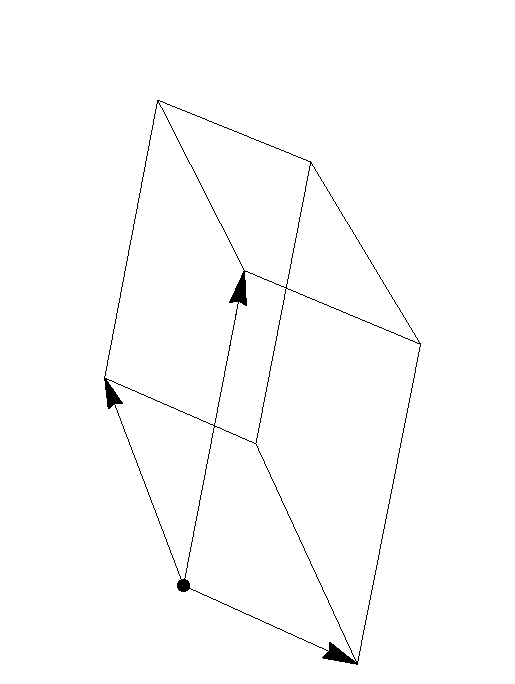
\includegraphics[width=\marginparwidth]{01-Arithmetic/support/det}

The determinant of a 3 by 3 matrix gives the volume of the parallelepiped created by using the columns of the matrix as the three parallel edges.} 
For a 3 by 3 matrix, the columns give the edges of a three dimensional parallelepiped and the determinant produces the volume of this object. The sign of the determinant is related to orientation. If you can use your right hand and place your index finger on the first vector, middle finger on the second vector, and thumb on the third vector, then the determinant is positive. 
\begin{example}
Consider the matrix $A = \begin{bmatrix}\cl{1\\0\\0}&\cl{0\\2\\0}&\cl{0\\0\\3}\end{bmatrix}$.  Starting from the origin, each column represents an edge of the rectangular box 
$0\leq x\leq 1$, 
$0\leq y\leq 2$, 
$0\leq z\leq 3$ with volume (and determinant) $V=lwh=(1)(2)(3)=6$. The sign of the determinant is positive because if you place your index finger pointing in the direction (1,0,0) and your middle finger in the direction (0,2,0), then your thumb points upwards in the direction (0,0,3). 
If you interchange two of the columns, for example 
$B = \begin{bmatrix}\cl{0\\2\\0}&\cl{1\\0\\0}&\cl{0\\0\\3}\end{bmatrix}$, then the volume doesn't change since the shape is still the same. However, the sign of the determinant is negative because if you point your index finger in the direction (0,2,0) and your middle finger in the direction (1,0,0), then your thumb points down in the direction (0,0,-3). If you repeat this with your left hand instead of right hand, then your thumb points up.
\end{example}

\subsection{Zero Determinants and Linear Dependence}
Because the determinant helps us find area in 2D, we can use this idea to help us understand when two vectors in 2D are linearly dependent.  
If two vectors are dependent, then one is a linear combination of the other, hence a multiple of the other.  
This means that the parallelogram formed by the two vectors has no area (as the two vectors lie on the same line).  
So if the vectors are dependent, the determinant is zero.  
Similarly, if the determinant is zero, then the vectors must lie on the same line and hence are linearly dependent.  
In 3D, three vectors being linearly dependent implies that one of the vectors lies in a plane or line spanned by the other two.
Any object in 3D that lies in a plane or line has no volume so the determinant is zero.  
Similarly, if the determinant of a 3 by 3 matrix is zero, then the column vectors must lie in the same plane and hence are linearly dependent. 
We now have a geometric interpretation for the key fact that
\marginpar{For a square matrix $A$, the following are equivalent:
\begin{enumerate}
	\item The determinant is zero.
	\item The columns are linearly dependent.
	\item The rref of $A$ is not $I$.
\end{enumerate}
}
\begin{quote}The determinant of a matrix is zero if and only if the columns are linearly dependent.\end{quote}
The homeworks asks you to compute determinants of matrices as well as row reduce them so that you can verify this fact in various settings. 
Notice that the columns of a square matrix are linearly independent if and only if the reduced row echelon form of the matrix is the identity matrix. 
This shows us that the determinant of a square matrix is nonzero if and only if the reduced row echelon form of the matrix is the identity matrix. 




\section{The Matrix Inverse}
Recall that the identity matrix $I$ behaves in matrix multiplication like the number 1 behaves in regular multiplication.  
When we solve the equation $ax=b$ with numbers, we multiply both sides by $a^{-1}$ to obtain $x=a^{-1}b=\frac{1}{a}b$. 
The multiplicative inverse of $a$ is simply $1/a$, because $a\frac1a=\frac1a a=1$.
We have been studying linear systems of the form {$A\vec x=\vec b$}. 
It would be nice if we could just divide both sides by {$A$}, but there is no such thing as division by a matrix in general. 
If we look only at square matrices, then sometimes it is possible to find a matrix {$B$} such that {$BA=AB=I$}, the identity matrix. 
If such a matrix {$B$} exists, then multiplying both sides of {$A\vec x = \vec b$} on the left by the matrix {$B$} yields $BA\vec x = B\vec B$, or $I\vec x = \vec x = B\vec b$. The matrix {$B$} is then called the \define[matrix!]{inverse} of {$A$}, and we write it as $A^{-1}$, the same symbol we used with regular multiplication. \marginpar{The solution to $A\vec x= \vec b$ is $\vec x=A^{-1}\vec b$, provided $A^{-1}$ exists.}When an inverse exists, the solution to $A\vec x = \vec b$ is simply $\vec x = A^{-1}\vec b$.

To find an inverse, we will start by considering a general 3 by 3 matrix. Once we are done, we will know how to find the inverse of any $n$ by $n$ matrix or state it does not exists.  
If an inverse exists, then write $A^{-1} = \begin{bmatrix}
c_{11}&c_{12}&c_{13}\\ 
c_{21}&c_{22}&c_{23}\\ 
c_{31}&c_{32}&c_{33} 
\end{bmatrix} $. Then the equation $AA^{-1}=I$ requires that the 3 matrix equations
$$A\begin{bmatrix} c_{11}\\ c_{21}\\c_{31}\end{bmatrix} = \begin{bmatrix} 1\\0\\0\end{bmatrix},
A\begin{bmatrix} c_{12}\\ c_{22}\\c_{32}\end{bmatrix} = \begin{bmatrix} 0\\1\\0\end{bmatrix},
A\begin{bmatrix} c_{13}\\ c_{23}\\c_{33}\end{bmatrix} = \begin{bmatrix} 0\\ 0\\1\end{bmatrix}$$
each have a solution, or that $(1,0,0), (0,1,0),$ and  $(0,0,1)$ are all linear combinations of the columns of $A$. This requires that we reduce all three augmented matrices
$$
\begin{bmatrix}[ccc|c]
a_{11}&a_{12}&a_{13}&1\\ 
a_{21}&a_{22}&a_{23}&0\\ 
a_{31}&a_{32}&a_{33}&0 
\end{bmatrix}
\quad\quad
\begin{bmatrix}[ccc|c]
a_{11}&a_{12}&a_{13}&0\\ 
a_{21}&a_{22}&a_{23}&1\\ 
a_{31}&a_{32}&a_{33}&0 
\end{bmatrix}
\quad\quad
\begin{bmatrix}[ccc|c]
a_{11}&a_{12}&a_{13}&0\\ 
a_{21}&a_{22}&a_{23}&0\\ 
a_{31}&a_{32}&a_{33}&1 
\end{bmatrix}.
$$
If the first three columns are all pivot columns, then the row operations required to reduce all three matrices will be identical, and none of the 4th columns will be pivot columns.  Rather than do three equivalent row reductions, we can solve all three simultaneously by creating the single augmented matrix 
$$\begin{bmatrix}[ccc|ccc]
a_{11}&a_{12}&a_{13}&1&0&0\\ 
a_{21}&a_{22}&a_{23}&0&1&0\\ 
a_{31}&a_{32}&a_{33}&0&0&1 
\end{bmatrix} $$\marginpar{A matrix $A_{n\times n}$ has an inverse if
\begin{enumerate}
	\item The columns of $A$ are linearly independent.
	\item The rank of $A$ is $n$
	\item The rref of $A$ is $I$.
	\item $|A|\neq 0$.
\end{enumerate}

It does not have an inverse if
\begin{enumerate}
	\item The columns of $A$ are linearly dependent.
	\item The rank is less than $n$
	\item The rref of $A$ is not $I$ (there is a row of zeros along the bottom).
	\item $|A|=0$.
\end{enumerate}
}or in compact form $\begin{bmatrix}[c|c]A &I\end{bmatrix}$. We now reduce this larger matrix to reduced row echelon form and obtain $\begin{bmatrix}[c|c]I &B\end{bmatrix}$, which tells us the coordinates of $(1,0,0)$, $(0,1,0),$ and  $(0,0,1)$ relative to the columns of $A$. 
The columns of the augmented portion $B$ on the right are the solutions to the three original systems, hence are the columns of $A^{-1}$.
To summarize, an inverse exists precisely if the augmented system $[A|I]$ reduces to $[I|A^{-1}]$. 
The the inverse matrix appears on the right after row reduction, provided the identity matrix appears on the left.
If the left block of the augmented matrix does not reduce to the identity matrix, then the matrix does not have an inverse.
If the left block does not reduce to the identity, then this implies that the original columns of $A$ are dependent.  
Later we will show that having an inverse is equivalent to having a nonzero determinant and having a rank which equals the number of columns. Remember that this is true for square matrices, or systems where we have the same number of equations as unknowns.

\begin{example}\label{ex inverse}
To find the inverse of 
$\begin{bmatrix} 1&2\\3&4\end{bmatrix}$ 
we reduce 
$\begin{bmatrix}[cc|cc] 1&2&1&0\\3&4&0&1\end{bmatrix}$.  
Reduction gives 
$\begin{bmatrix}[cc|cc] 1&0&-2&1\\0&1&3/2&-1/2
\end{bmatrix}$. 
The inverse is the right block  
$ \begin{bmatrix} -2&1\\3/2&-1/2
\end{bmatrix}$. 
\marginpar{Examples involving larger matrices are in the homework. Remember that you can solve systems by finding an inverse of the coefficient matrix.}
You can always check your result by computing $AA^{-1}$ to see if it is $I$, for example
$\begin{bmatrix} 1&2\\ 3&4\end{bmatrix} \begin{bmatrix} -2&1\\3/2&-1/2\end{bmatrix} 
=  \begin{bmatrix} 1&0\\0&1
\end{bmatrix}$. 
Using this inverse, the solution to the system 
$\begin{cases}1x+2y=4\\3x+4y=0\end{cases}$ is $A^{-1}\vec b 
= \begin{bmatrix} -2&1\\3/2&-1/2\end{bmatrix}
\begin{bmatrix}4\\0\end{bmatrix} 
=  \begin{bmatrix}-8\\6\end{bmatrix}$.
\end{example}


\section{Eigenvalues and Eigenvectors}
Let's start by looking at an example to motivate the language we are about to introduce.  Consider the matrix
$A=\begin{bmatrix} 2&1\\1&2\end{bmatrix} $.  When we multiply this matrix by the vector 
$\vec x = \begin{bmatrix} 1\\1\end{bmatrix} $, 
we obtain 
$\begin{bmatrix} 2&1\\1&2\end{bmatrix} \begin{bmatrix} 1\\1\end{bmatrix} = \begin{bmatrix} 3\\3\end{bmatrix}=3\vec x$. Multiplication by the matrix $A$ was miraculously the same as multiplying by the number 3. Symbolically we have $A\vec x = 3\vec x$. 
Not every vector $\vec x$ satisfies this property, for by 
$\vec x = \begin{bmatrix} 1\\0\end{bmatrix} $ 
gives  
$\begin{bmatrix} 2&1\\1&2\end{bmatrix} \begin{bmatrix} 1\\0\end{bmatrix} = \begin{bmatrix} 2\\1\end{bmatrix}$, which is not a multiple of $\vec x = \begin{bmatrix} 1\\0\end{bmatrix} $. Our main goal in this section is to answer the following two questions:
\begin{enumerate}
	\item For which nonzero vectors $\vec x$ (eigenvectors) is it possible to write $A\vec x = \lambda \vec x$?
	\item Which scalars $\lambda$ (eigenvalues) satisfy $A\vec x = \lambda \vec x$?
\end{enumerate}

Now for some definitions. 
Let $A$ be a square $n\times n$ matrix. 
An \definemargin{eigenvector} is a nonzero vector $\vec x$ such that $A\vec x =\lambda \vec x$ (matrix multiplication reduces to scalar multiplication) for some scalar {$\lambda$} called an \definemargin{eigenvalue}.
We avoid letting $\vec x$ be the zero vector because $A\vec 0=\lambda \vec 0$ no matter what $\lambda$ is.
We can rewrite the equation $A\vec x = \lambda \vec x$ as $\vec 0 = A\vec x-\lambda \vec x = A\vec x-\lambda I \vec x$ and then factor to obtain $$(A-\lambda I)\vec x=\vec 0.$$ 
In other words, we need to find a $\lambda$ so that there are nonzero solutions to the homogeneous system of equations, or equivalently we need to pick a $\lambda$ so that the columns of $A-\lambda I$ are linearly dependent. 
With the correct $\lambda$, we know that $A-\lambda I$ has no inverse, and so it also means that $\det(A-\lambda I)=0$. 
This last equation is the key equation we will solve, since it does not contain the vector $\vec x$ anymore. 
The expression {$\det(A-\lambda I)$} is called the \definemargin{characteristic polynomial} of {$A$}.
It is a polynomial of degree {$n$}, and hence there are at most {$n$} eigenvalues (which correspond to the zeros of the polynomial). 
To find the eigenvalues and eigenvectors, we 
\begin{enumerate}
	\item solve $\det(A-\lambda I) = 0$ to obtain the eigenvalues, and then
	\item for each eigenvalue, we solve $(A-\lambda I)\vec x=\vec 0$ to obtain the eigenvectors.
\end{enumerate}
As a way to check your work, the following two facts can help.
\begin{itemize}
	\item \marginpar{The trace and determinant are equal to the sum and product of the eigenvalues.
	}The sum of the eigenvalues equals the trace of the matrix (the sum of the diagonal elements).
	\item The product of the eigenvalues equals the determinant.
\end{itemize}

\begin{example} \label{ex eigen1}
To find the eigenvalues of {$\begin{bmatrix} 2&1\\1&2\end{bmatrix} $}, first subtract $\lambda$ from each diagonal entry {$\begin{bmatrix} 2-\lambda&1\\1&2-\lambda\end{bmatrix} $}, and then find the determinant. Factor to get {$(2-\lambda)(2-\lambda)-1 = \lambda^2-4\lambda+3=(\lambda-1)(\lambda-3)$}. The zeros are 1 and 3, so the eigenvalues are {$\lambda=1,3$}. As a check, the trace of this matrix is $2+2=4$ and the sum of the eigenvalues is $1+3$. In addition, the determinant is $4-1=3$ which equals the product of the eigenvalues.  

When {$\lambda=1$}, we compute {$A-\lambda I =\begin{bmatrix} 1&1\\1&1\end{bmatrix} $}. We solve the equation  {$(A-\lambda I )\vec x=0$} by reducing the augmented matrix $\begin{bmatrix}[cc|c] 1&1&0\\1&1&0\end{bmatrix} $ to its rref $\begin{bmatrix}[cc|c] 1&1&0\\0&0&0\end{bmatrix} $.\marginpar{Since we are solving a homogeneous system $A\vec x = \vec 0$, we could avoid writing the last column of zeros.} Since $x_2$ is a free variable, we solve $x_1+x_2=0$ for $x_1$ to obtain the equations $x_1=-x_2$, $x_2=x_2$, and then write our solution in vector form 
$\begin{bmatrix} x_1\\x_2\end{bmatrix}= x_2\begin{bmatrix} -1\\1\end{bmatrix}$
 for some {$x_2\neq 0$} . There are infinitely many eigenvectors corresponding to $\lambda=1$. A particular eigenvector is  $\begin{bmatrix} -1\\1\end{bmatrix} $ and all the rest are a linear combination of this one. 

When {$\lambda=3$}, we compute {$A-\lambda I =\begin{bmatrix} -1&1\\1&-1\end{bmatrix} $}. Reducing  
$\begin{bmatrix}[cc|c] -1&1&0\\1&-1&0\end{bmatrix}$ gives
$\begin{bmatrix}[cc|c] 1&-1&0\\0&0&0\end{bmatrix}$, which means the eigenvectors are of the form $x_2\begin{bmatrix} 1\\1\end{bmatrix} $ for some {$x_2\neq 0$}. A particular eigenvector corresponding to $\lambda=3$ is $\begin{bmatrix} 1\\1\end{bmatrix} $, and all others are a linear combination of this one.
\end{example}

Finding eigenvalues and eigenvectors requires that we compute determinants, find zeros of polynomials, and then solve homogeneous systems of equations. You know you are doing the problem correctly if you get infinitely many solutions to the system $(A-\lambda I)\vec x=0$ for each lambda (i.e. there is at least one row of zeros along the bottom).

Eigenvalues and eigenvectors show up in many different places in engineering, computer science, physics, chemistry, and mathematics. We will be exploring how eigenvectors appear throughout linear algebra 
%and differential equations 
as the semester progresses.  For now we'll just focus on being able to find them.

\begin{example}\label{eigenvalueexample3} \label{ex eigen2}
Let's find the eigenvalues and eigenvectors of the matrix 
$A=\begin{bmatrix}2&1&4\\ 1&2&4\\ 0&0&1\end{bmatrix}$. 
Subtracting $\lambda$ from the diagonals gives 
$\begin{bmatrix}2-\lambda&1&4\\ 1&2-\lambda&4\\ 0&0&1-\lambda\end{bmatrix}$. The determinant of this matrix is easiest to compute if you expand along the third row to get $0 - 0 + (1-\lambda) \begin{vmatrix} 2-\lambda&1\\1&2-\lambda\end{vmatrix}$. Computing the 2 by 2 determinant gives $(1-\lambda)[(2-\lambda)(2-\lambda)-1] = (1-\lambda)(\lambda-1)(\lambda-3)$,  so the eigenvalues are $1,1,3$ (1 is a repeated root). As a check, their sum is $1+1+3=5$ and the trace of $A$ is $2+2+1=5$ as well. For larger matrices, determinants are not always easy to check, so just checking the trace is a fast way to make sure you are on the right path.

When $\lambda=1$, we compute $A-\lambda I =\begin{bmatrix}1&1&4\\ 1&1&4\\ 0&0&0\end{bmatrix} $. Reducing the system  $(A-\lambda I )\vec x=0$ yields $\begin{bmatrix}[ccc|c]1&1&4&0\\ 0&0&0&0\\ 0&0&0&0\end{bmatrix}$, which has two free variables. The solution is $\begin{bmatrix} x_1\\x_2\\ x_3\end{bmatrix} = x_2\begin{bmatrix} -1\\1\\0\end{bmatrix}+x_3\begin{bmatrix} -4\\0\\1\end{bmatrix} $. Hence the eigenvectors are nonzero linear combinations of $\begin{bmatrix} -1\\1\\0\end{bmatrix}$ and $\begin{bmatrix} -4\\0\\1\end{bmatrix}$. Notice that all the eigenvectors can be obtained as linear combinations of two linearly independent eigenvectors, in part because $\lambda =1$ is a double root of the characteristic polynomial. 

When $\lambda=3$, we compute $A-\lambda I =\begin{bmatrix}-1&1&4\\ 1&-1&4\\ 0&0&-2\end{bmatrix}$. Next, reducing $\begin{bmatrix}[ccc|c]-1&1&4&0\\ 1&-1&4&0\\ 0&0&-2&0\end{bmatrix}$ yields $\begin{bmatrix}[ccc|c]-1&1&0&0\\ 0&0&1&0\\ 0&0&0&0\end{bmatrix} $, which has only one free variable . The solution is $\begin{bmatrix} x_1\\x_2\\ x_3\end{bmatrix} = x_2\begin{bmatrix} 1\\1\\0\end{bmatrix}$. The eigenvectors are nonzero linear combinations of $\begin{bmatrix} 1\\1\\0\end{bmatrix}$. Because $\lambda=3$ is a single root of the characteristic polynomial, all the eigenvectors can be obtained as linear combinations of one eigenvector.
\end{example}

\newgeometry{left=1in,right=1in,top=1in,bottom=1in}
\newpage

\section{Preparation}

\noindent
This chapter covers the following ideas. When you create your lesson plan, it should contain examples which illustrate these key ideas. Before you take the quiz on this unit, meet with another student out of class and teach each other from the examples on your lesson plan. 


\begin{enumerate}

\item Be able to use and understand matrix and vector notation, addition, scalar multiplication, the dot product, matrix multiplication, and matrix transposition. 
\item Use Gaussian elimination to solve systems of linear equations and write the solution in parametric and vector form. Define and use the words homogeneous, nonhomogeneous, row echelon form, and reduced row echelon form. 
\item Find the rank of a matrix. Determine if a collection of vectors is linearly independent. If linearly dependent, be able to write vectors as linear combinations of the preceding vectors.
\item For square matrices, compute determinants, inverses, eigenvalues, and eigenvectors. 
\item Illustrate with examples how a nonzero determinant is equivalent to having independent columns, an inverse, and nonzero eigenvalues. Similarly, a zero determinant is equivalent to having dependent columns, no inverse, and a zero eigenvalue. 

\end{enumerate}

%%% Local Variables: 
%%% mode: latex
%%% TeX-master: "../linear-algebra"
%%% End: 


Here are the preparation problems for this unit.  All of these problems come from this book (not Schaum's Outlines).  Remember that solutions appear at the end of each chapter.

%Day 1 we'll only look at matrix multiplication in class.  I'll introduce vector addition, scalar multiplication, the dot product, and then go to linear combinations. This leads immediately to matrix multiplication. Next we will focus on systems of equations and how to solve them.  I'll show how systems can be written in 4 ways, and then reduce a 2 by 2 system.  The next day we will focus on larger systems, and introduce rank and independence.  The next day I'll add in determinants and inverses, and hopefully get to eigenvalues and eigenvectors.   


\begin{center}
\begin{tabular}{ll|l}
\multicolumn{2}{c}{Preparation Problems (\href{http://ilearn.byui.edu/bbcswebdav/institution/Physical\_Sci\_Eng/Mathematics/Personal\%20Folders/WoodruffB/341/1-Arithmetic-Preparation-Solutions.pdf}{click for solutions})}
&
Webcasts 
(
\href{http://ilearn.byui.edu/bbcswebdav/institution/Physical\_Sci\_Eng/Mathematics/Personal\%20Folders/WoodruffB/341/1-Arithmetic-videos.pdf}{pdf copy}
)\\
\hline\hline
Day 1&
1c,
2h,
2o,
3b
&
\href{http://ilearn.byui.edu/bbcswebdav/institution/Physical\_Sci\_Eng/Mathematics/Personal\%20Folders/WoodruffB/341/1-Arithmetic-video-01.wmv}{1},
\href{http://ilearn.byui.edu/bbcswebdav/institution/Physical\_Sci\_Eng/Mathematics/Personal\%20Folders/WoodruffB/341/1-Arithmetic-video-02.wmv}{2},
\href{http://ilearn.byui.edu/bbcswebdav/institution/Physical\_Sci\_Eng/Mathematics/Personal\%20Folders/WoodruffB/341/1-Arithmetic-video-03.wmv}{3}
\\ \hline
Day 2&
4c,
4e,
4f,
5a
&
\href{http://ilearn.byui.edu/bbcswebdav/institution/Physical\_Sci\_Eng/Mathematics/Personal\%20Folders/WoodruffB/341/1-Arithmetic-video-04.wmv}{4},
\href{http://ilearn.byui.edu/bbcswebdav/institution/Physical\_Sci\_Eng/Mathematics/Personal\%20Folders/WoodruffB/341/1-Arithmetic-video-05.wmv}{5},
\href{http://ilearn.byui.edu/bbcswebdav/institution/Physical\_Sci\_Eng/Mathematics/Personal\%20Folders/WoodruffB/341/1-Arithmetic-video-06.wmv}{6}
\\ \hline
Day 3&
5c,
6a,
6b,
7d
&
\href{http://ilearn.byui.edu/bbcswebdav/institution/Physical\_Sci\_Eng/Mathematics/Personal\%20Folders/WoodruffB/341/1-Arithmetic-video-07.wmv}{7},
\href{http://ilearn.byui.edu/bbcswebdav/institution/Physical\_Sci\_Eng/Mathematics/Personal\%20Folders/WoodruffB/341/1-Arithmetic-video-08.wmv}{8}
\\ \hline
Day 4&
7h,
7l,
8b,
8j 
&
\href{http://ilearn.byui.edu/bbcswebdav/institution/Physical\_Sci\_Eng/Mathematics/Personal\%20Folders/WoodruffB/341/1-Arithmetic-video-09.wmv}{9},
\href{http://ilearn.byui.edu/bbcswebdav/institution/Physical\_Sci\_Eng/Mathematics/Personal\%20Folders/WoodruffB/341/1-Arithmetic-video-10.wmv}{10}
\\ \hline
Day 5&
9b,
10e,
10g,
10h
&
\href{http://ilearn.byui.edu/bbcswebdav/institution/Physical\_Sci\_Eng/Mathematics/Personal\%20Folders/WoodruffB/341/1-Arithmetic-video-11.wmv}{11}
\\ \hline
Day 6&
11, 
Lesson Plan,
Quiz &
\\ \hline
\end{tabular}
\end{center}

Please download and print all the problems. I have tried to keep the text short and readable, and I want you to read the text (reading 3-4 pages for every day of class will get you through the whole book). If you find errors or find some parts hard to read, please email me so that I can improve the text.




The problems listed below are found in the subsequent pages. The suggested problems are a minimal set of problems that I suggest you complete.
\begin{center}
\begin{tabular}{|l|l|l|l|l|}
\hline
Concept&Suggestions&Relevant Problems\\ \hline
Basic Notation&1bcf,2abehln&1,2\\ \hline
Gaussian Elimination&3all,4acf&3,4\\ \hline
Rank and Independence&5ac,6bd&5,6\\ \hline
Determinants&7adgh&7\\ \hline
Inverses&8ag,9ac&8,9\\ \hline
Eigenvalues&10abdghi&10\\ \hline
Summarize&11(multiple times)&11\\ \hline
\end{tabular}
\end{center}


%%% Local Variables: 
%%% mode: latex
%%% TeX-master: "../linear-algebra"
%%% End: 




\section{Problems}


\begin{enumerate}


\item \textbf{Vector Arithmetic:} For each pair of vectors, (1) find the length of each vector, (2) compute the dot product of the vectors, (3) find the cosine of the angle between them, and (4) determine if the vectors are orthogonal.
\begin{enumerate}
\begin{multicols}{3}
	\item $(1,2), (3,4)$
	\item $[-2~1], [4~-8]$
	\item $(1,2,2), (3,0,-4)$
	\item $\left<-2,3,5\right>, \left<4,-4,4\right>$
	\item $[1~1~1~1], [2~3~-4~-1]$
	\item $[1~-4~3~0~2]^T, [2~1~0~10~1]^T$
\end{multicols}
\end{enumerate}
More problems are in Schaum's Outlines - 
Chapter 1:1-13,  54-66.
\item \textbf{Matrix Arithmetic:} Consider the matrices
$$
A=
\begin{bmatrix}
 1 & 2 \\
 3 & 4
\end{bmatrix}
,
B=
\begin{bmatrix}
 4 & -1 \\
 3 & 2
\end{bmatrix}
,
C=
\begin{bmatrix}
 1 & 0 & -1 \\
 2 & 3 & 4
\end{bmatrix}
,
D=
\begin{bmatrix}
 0 & 2 & 1 \\
 3 & 0 & 4 \\
 -1 & 1 & 2
\end{bmatrix}
, \text{ and }
E=
\begin{bmatrix}
 3 \\
 1 \\
 -4
\end{bmatrix}.
$$
Compute each of the following, or explain why it is not possible.
\begin{enumerate}
\begin{multicols}{4}
	\item $A+B$ and $3A-2B$
	\item $AB$ and $BA$
	\item $AC$ and $CA$
	\item $BC$ and $CB$
	\item $CD$ and $DC$
	\item $DE$ and $ED$
	\item $CDE$
	\item $CC^T$ and $C^TC$
	\item $DC^T$ and $CD^T$
	\item $AB$ and $B^TA^T$
	\item $BA$ and $A^TB^T$
	\item Trace of $A$, $B$, $D$.	
\end{multicols}
\end{enumerate}
For each of the following, compute the product in three ways (1) using linear combinations of columns, (2) using rows dotted by columns, and (3) using linear combinations of rows (see Table \ref{matrixmult}).
\begin{multicols}{4}
\begin{enumerate}[resume]
\item $AB$
\item $BC$
\item $CD$
\item $DE$
\end{enumerate}
\end{multicols}
More problems are in Schaum's Outlines - 
Chapter 1:14-26, 67-79;
Chapter 3:1-3, 68-70.






\item \textbf{Interpreting RREF:} Each of the following augmented matrices requires one row operation to be in reduced row echelon form. Perform the required row operation, and then write the solution to corresponding system of equations in terms of the free variables.
\begin{multicols}{3}
\begin{enumerate}
	\item 
$
\begin{bmatrix}[ccc|c]
 1 & 0 & 0 & 3 \\
 0 & 0 & 1 & 1 \\
 0 & 1 & 0 & -2
\end{bmatrix}
$
	\item 
$
\begin{bmatrix}[ccc|c]
 1 & 2 & 0 & -4 \\
 0 & 0 & 1 & 3 \\
 -3 & -6 & 0 & 12
\end{bmatrix}
$
	\item 
$
\begin{bmatrix}[ccc|c]
 0 & 1 & 0 & 4 \\
 0 & 0 & 5 & 15 \\
 0 & 0 & 0 & 0
\end{bmatrix}
$
	\item 
$
\begin{bmatrix}[ccc|c]
 1 & 0 & 2 & 4 \\
 0 & 1 & -3 & 0 \\
 0 & 0 & 0 & 1
\end{bmatrix}
$
	\item 
$
\begin{bmatrix}[ccccc|c]
 0 & 1 & 0 & 7 & 0 & 3 \\
 0 & 0 & 1 & 5 & -3 & -10 \\
 0 & 0 & 0 & 0 & 1 & 2 \\
 0 & 0 & 0 & 0 & 0 & 0
\end{bmatrix}
$
\end{enumerate}
\end{multicols}

More problems are in Schaum's Outlines - 
Chapter 2:37-40


\item \textbf{Solving Systems with Gaussian Elimination:} Solve each system of equations using Gaussian elimination, by reducing the augmented matrix to reduced row echelon form (rref).
\begin{multicols}{3}
\begin{enumerate}
	\item 
$
\begin{array}{rl}
 x  -3y &= 10 \\
 3x +2y &= 8
\end{array}
$


	\item 
$
\begin{array}{rl}
 2x+ 6y -z &= 9 \\
 x+ 3y -3z &= 17
\end{array}
$


	\item 
$
\begin{array}{rl}
  x_2 -2x_3 &= -5 \\
 2x_1 -x_2 + 3x_3 &= 4 \\
 4x_1 +x_2 + 4x_3 &= 5
\end{array}
$


	\item 
$
\begin{array}{rl}
 x_1 + 2x_3 &= -2 \\
 2x_1  -3x_2  &= -3 \\
 3x_1 +x_2 -x_3 &= 2
\end{array}
$


	\item 
$
\begin{array}{rl}
 2x_1 +x_2 + 4x_3 &= -1 \\
 -x_1 + 3x_2 + 5x_3 &= 2 \\
 x_2 + 2x_3 &= -2
\end{array}
$


	\item 
$
\begin{array}{rl}
 x_1 -2x_2 +x_3 &= 4 \\
 -x_1 + 2x_2 + 3x_3 &= 8 \\
 2x_1  -4x_2 +x_3 &= 5
\end{array}
$


	\item 
$
\begin{array}{rl}
 x_1 + 2x_3 + 3x_4 &= -7 \\
 2x_1 +x_2 + 4x_4 &= -7 \\
 -x_1 + 2x_2 + 3x_3  &= 0 \\
 x_2  -2x_3  -x_4 &= 4
\end{array}
$
\end{enumerate}
\end{multicols}

More problems are in Schaum's Outlines - 
Chapter 2:
44-48, 51-56, 70-72, 75-28, 86-90 






\item \textbf{Rank and Linear Dependence:} Compute the rank of each matrix. Use this result to determine if the columns are linearly dependent. If the vectors are dependent, write each non pivot column as a linear combination of the pivot columns.
\begin{multicols}{4}
\begin{enumerate}
	\item \label{rank1} 
$
\begin{bmatrix}
 1 & 2 & 3 \\
 4 & -2 & 1 \\
 3 & 0 & 4
\end{bmatrix}
$

	\item \label{rank2}
$
\begin{bmatrix}
 1 & -1 & -1 \\
 -2 & 3 & 5 \\
 3 & 1 & 9
\end{bmatrix}
$

	\item 
$
\begin{bmatrix}
 1 & 3 & -1 & 9 \\
 -1 & -2 & 0 & -5 \\
 2 & 1 & 3 & -2
\end{bmatrix}
$

	\item \label{rank4}
$
\begin{bmatrix}
 1 & 3 & 12 & 1 \\
 2 & 0 & -6 & 3 \\
 -1 & 1 & 8 & -4 \\
 0 & 2 & 10 & 2
\end{bmatrix}
$

\end{enumerate}
\end{multicols}

More problems are in Schaum's Outlines - 
Chapter 5:
19, 20, 22, 68.





\item \textbf{Linear Independence:} In each problem, determine if the vectors given are linearly independent. If the vectors are linearly dependent, write one of the vectors as a linear combination of the others.
\begin{multicols}{2}
\begin{enumerate}
	\item \,
	$[2, -1, 0]$, $[1, 0, 3]$, $[3, 2, 4]$

	\item \,
$[1, 2, -3, 4], [3, -2, -1, -2], [5, -2, -3, -1]$

	\item \,
$[0, 1, 1, 1], [1, 0, 1, 1], [1, 1, 0, 1], [1, 1, 1, 0]$

	\item \,
$[1, 0, -1, -2], [1, 2, 3, 0], [0, 1, -1, 2], [2, 0, 1, -5]$
\end{enumerate}
\end{multicols}

More problems are in Schaum's Outlines - 
Chapter 5:
1, 3, 4, 50, 53.


\item \textbf{Determinants:} Find the determinant of each matrix. For 3 by 3 matrices, compute the determinant in 2 different ways by using a cofactor expansion along a different row or column. 
\begin{enumerate}
\begin{multicols}{3}
	\item 
$
\begin{bmatrix}
 1 & 2 \\
 3 & 4
\end{bmatrix}
$
	\item 
$
\begin{bmatrix}
 4 & 3 \\
 5 & 9
\end{bmatrix}
$
	\item 
$
\begin{bmatrix}
 2 & 1 & 0 \\
 0 & 2 & 1 \\
 1 & 0 & 2
\end{bmatrix}
$
	\item 
$
\begin{bmatrix}
 3 & 1 & -2 \\
 1 & -1 & 4 \\
 2 & 2 & 1
\end{bmatrix}
$
	\item 
$
\begin{bmatrix}
 2 & 3 & -1 \\
 1 & 0 & 0 \\
 4 & 2 & 5
\end{bmatrix}
$
	\item 
$
\begin{bmatrix}
 5 & 1 & -3 \\
 2 & -1 & 2 \\
 1 & 4 & -1
\end{bmatrix}
$
	\item 
$
\begin{bmatrix}
 2 & 1 & -6 & 8 \\
 0 & 3 & 5 & 4 \\
 0 & 0 & 1 & 5 \\
 0 & 0 & 0 & -4
\end{bmatrix}
$
	\item 
$
\begin{bmatrix}
 3 & 2 & 5 & -1 \\
 0 & 8 & 4 & 2 \\
 0 & -1 & 0 & 0 \\
 0 & -5 & 3 & -1
\end{bmatrix}
$
	\item 
$
\begin{bmatrix}
 1 & 1 & 1 & 1 \\
 2 & -1 & 1 & 1 \\
 -1 & 1 & 2 & -2 \\
 1 & 1 & -1 & -1
\end{bmatrix}
$
	\item 
$
\begin{bmatrix}
 1 & 1 & 1 & 1 \\
 2 & 2 & 2 & 2 \\
 0 & 2 & 1 & -1 \\
 1 & 0 & -2 & 1
\end{bmatrix}
$
\end{multicols}
\end{enumerate}

For the following matrices, compute the determinant and use your answer to determine if the columns are linearly independent.
\begin{enumerate}[resume]
\begin{multicols}{3}
	\item Use the matrix from \ref{rank1}
	\item Use the matrix from \ref{rank2}
	\item Use the matrix from \ref{rank4}
\end{multicols}
\end{enumerate}

More problems are in Schaum's Outlines -  
Chapter 10:
1-6, 21, 23, 51-55






\item \textbf{Inverse:} Find the inverse of each matrix below.
\begin{multicols}{4}
\begin{enumerate}
	\item \label{inv1}
$
\begin{bmatrix}
 1 & 2 \\
 3 & 4
\end{bmatrix}
$
	\item \label{inv2}
$
\begin{bmatrix}
 -2 & 4 \\
 3 & -5
\end{bmatrix}
$
	\item 
$
\begin{bmatrix}
 0 & 1 \\
 -1 & 0
\end{bmatrix}
$
	\item 
$
\begin{bmatrix}
 2 & 3 \\
 4 & 5
\end{bmatrix}
$
	\item 
$
\begin{bmatrix}
 7 & 3 \\
 2 & 1
\end{bmatrix}
$
	\item 
$
\begin{bmatrix}
 1 & 0 & 2 \\
 0 & 1 & 0 \\
 0 & 0 & 4
\end{bmatrix}
$
	\item \label{inv3}
$
\begin{bmatrix}
 1 & 0 & 2 \\
 0 & 1 & 0 \\
 -1 & 1 & 4
\end{bmatrix}
$
	\item 
$
\begin{bmatrix}
 3 & 0 & 3 \\
 0 & -1 & 1 \\
 0 & 3 & -4
\end{bmatrix}
$
	\item 
$
\begin{bmatrix}
 1 & 2 & -1 \\
 2 & 3 & -2 \\
 0 & 3 & 2
\end{bmatrix}
$
	\item \label{inv4}
$
\begin{bmatrix}
 -2 & 0 & 5 \\
 -1 & 0 & 3 \\
 4 & 1 & -1
\end{bmatrix}
$
	\item 
$
\begin{bmatrix}
 2 & 1 & 1 \\
 1 & 2 & 1 \\
 1 & 1 & 2
\end{bmatrix}
$
	\item 
$
\begin{bmatrix}
a & b\\
c & d
\end{bmatrix}
$
\end{enumerate}
\end{multicols}




More problems are in Schaum's Oultines:
Chapter 3: 7-11, 77-80.


\item \textbf{Solve systems using an inverse:} Solve each system by using an inverse from above.
\begin{multicols}{2}
\begin{enumerate}
	\item 
$\left\{
\begin{array}{rl}
 x_1 + 2x_2  &=3\\
 3x_1 + 4x_2  &=4
\end{array}
\right.$ using \ref{inv1}.
	\item 
$\left\{
\begin{array}{rl}
 -2x_1 + 4x_2  &=4\\
 3x_1  -5x_2  &=-2
\end{array}
\right.$ using \ref{inv2}.
	\item 
$\left\{
\begin{array}{rl}
 1x_1 + 2x_3 &=2\\
 x_2 &=3\\
 -x_1 +x_2 + 4x_3  &=1
\end{array}
\right.$ using \ref{inv3}.
	\item 
$\left\{
\begin{array}{rl}
 -2x_1+ 5x_3 &=-2\\
 -x_1+ 3x_3 &=1\\
 4x_1 +x_2  -x_3 &=3
\end{array}
\right.$ using \ref{inv4}.
\end{enumerate}
\end{multicols}

Now grab any problem from the entire unit that involves solving a system where an inverse applies.  Find the inverse of the coefficient matrix and use it to find the solution. (Use the solutions at the back to select a problem with a unique solution).



\item \textbf{Eigenvalues and Eigenvectors:} For each matrix, compute the characteristic polynomial and eigenvalues. For each eigenvalue, give all the corresponding eigenvectors. Remember that you can check your answer by comparing the trace to the sum of the eigenvalues, and the determinant to the product of the eigenvalues.
\begin{multicols}{4}
\begin{enumerate}
	\item 
$
\begin{bmatrix}
 1 & 2 \\
 0 & 3
\end{bmatrix}
$
	\item 
$
\begin{bmatrix}
 0 & 1 \\
 -1 & -2
\end{bmatrix}
$
	\item 
$
\begin{bmatrix}
 2 & 3 \\
 3 & 2
\end{bmatrix}
$
	\item 
$
\begin{bmatrix}
 0 & 1 \\
 -1 & 0
\end{bmatrix}
$
	\item 
$
\begin{bmatrix}
 1 & 4 \\
 2 & 3
\end{bmatrix}
$
	\item 
$
\begin{bmatrix}
 3 & 1 \\
 4 & 6
\end{bmatrix}
$
	\item 
$
\begin{bmatrix}
 1 & 2 & 2 \\
 0 & 1 & 2 \\
 0 & 0 & 1
\end{bmatrix}
$
	\item 
$
\begin{bmatrix}
 1 & 2 & 2 \\
 0 & 1 & 0 \\
 0 & 0 & 1
\end{bmatrix}
$
	\item 
$
\begin{bmatrix}
 3 & 0 & 0 \\
 0 & 2 & 1 \\
 0 & 1 & 2
\end{bmatrix}
$
	\item 
$
\begin{bmatrix}
 1 & 1 & 0 \\
 0 & 2 & 0 \\
 0 & 1 & 1
\end{bmatrix}
$
\end{enumerate}
\end{multicols}
 
More problems are in Schaum's Outlines - 
(only worry about the eigenvalues and eigenvectors part of each problem - ignore diagonalization questions)
Chapter 11: 9, 10, 11, 17, 18, 20, 57, 58, 59, 60



\item At this point, you are ready to make your own examples. Create your own 2 by 2 or 3 by 3 matrix $A$.
\begin{itemize}
\begin{multicols}{2}
	\item Find rref $A$.
	\item Find the rank of $A$.
	\item Are the columns of $A$ independent?
	\item Compute $|A|$.
	\item Compute $A^{-1}$ (or explain why not possible).
	\item Find the eigenvalues and eigenvectors of $A$.
\end{multicols}
\end{itemize}
For a 3 by 3 matrix, the eigenvalues and eigenvectors may be hard to find by hand (so use technology).
Use technology to check your work by hand. The first column of questions applies to all matrices (square or not), whereas the last column only makes sense when the matrix is square. For a 2 by 2 matrix, you can always compute the eigenvalues using the quadratic formula, which may result in irrational or complex eigenvalues. 

Repeat this exercise a few times with various types of matrices (diagonal, triangular, symmetric, skew-symmetric). Do you notice any patterns? If you pick larger matrices, you can do everything except the eigenvalues and eigenvectors by hand. Once you feel comfortable with the computations by hand, move to a computer and start using larger matrices to find patterns. 
 


\end{enumerate}



\section{Projects}
The following projects require you to use technology to further explore a topic from this unit. Use a computer algebra system (CAS) to perform your computations so you can save your work and quickly modify things as needed. 

\begin{enumerate}
	\item A matrix and its transpose $A^T$ have some common properties. Your job in this project is to explore the relationships between a matrix and its transpose.	
	
\begin{enumerate}
	\item Start by choosing your own 4 by 4 matrix.  For both $A$ and $A^T$, compute the rref, rank, determinant, inverse, eigenvalues, and eigenvectors. Which are the same? 
	\item Change your matrix to some other 4 by 4 or larger matrix and repeat the computations. 
	\item Based on these two examples, which quantities do you think will be always be the same for $A$ and $A^T$? 
	\item Try creating an ugly large matrix and see if your conjecture is correct. While examples are not proofs that a conjecture is true, examples do provide the foundation upon which all mathematical theorems are built.  New ideas always stem from examples.
	\item What happens if a matrix is not square? Select your own non square matrix (such as 3 by 4). Compute the rref of both $A$ and $A^T$, as well as the rank. 
	\item Change the matrix and repeat this computation. What conjecture should you make?
\end{enumerate}
\end{enumerate}








\section{Solutions}




\begin{multicols}{2}
\begin{enumerate}
\small
\item \textbf{Vector Arithmetic:}
\begin{enumerate}
	\item $\sqrt{5}, 5, 11, \cos\theta = \frac{11}{5\sqrt{5}}$, No
	\item $\sqrt{5}, 2\sqrt{5}, 0, \cos\theta = 0$, Yes
	\item $3, 5, -5, \cos\theta = -\frac{1}{3}$, No
	\item $\sqrt{38}, 4\sqrt{3}, 0, \cos\theta = 0$, Yes
	\item $2, \sqrt{30}, 0, \cos\theta = 0$, Yes
	\item $\sqrt{30}, \sqrt{106}, 0, \cos\theta = 0$, Yes
\end{enumerate}
\item \textbf{Matrix Arithmetic:}
%\begin{multicols}{4}
\begin{enumerate}
	\item $ 
\begin{bmatrix}
5 & 1 \\
 6 & 6
\end{bmatrix}
$, $
\begin{bmatrix}
 -5 & 8 \\
 3 & 8
\end{bmatrix}
$
	\item 
$
\begin{bmatrix}
 10 & 3 \\
 24 & 5
\end{bmatrix}
$, 
$
\begin{bmatrix}
 1 & 4 \\
 9 & 14
\end{bmatrix}
$
	\item 
	$
\begin{bmatrix}
 5 & 6 & 7 \\
 11 & 12 & 13
\end{bmatrix}
$, $CA$ not possible
	\item 
	$
\begin{bmatrix}
 2 & -3 & -8 \\
 7 & 6 & 5
\end{bmatrix}
$, $CB$ not possible
	\item 
	$
\begin{bmatrix}
 1 & 1 & -1 \\
 5 & 8 & 22
\end{bmatrix}
$, $DC$ not possible
	\item 
	$
\begin{bmatrix}
 -2 \\
 -7 \\
 -10
\end{bmatrix}
$, $ED$ not possible
	\item $
\begin{bmatrix}
 8 \\
 -65
\end{bmatrix}
$
	\item 
$\begin{bmatrix}
 2 & -2 \\
 -2 & 29
\end{bmatrix}$, 
$
\begin{bmatrix}
 5 & 6 & 7 \\
 6 & 9 & 12 \\
 7 & 12 & 17
\end{bmatrix}
$
	\item 
$\begin{bmatrix}
 -1 & 10 \\
 -1 & 22 \\
 -3 & 9
\end{bmatrix}
$, $
\begin{bmatrix}
 -1 & -1 & -3 \\
 10 & 22 & 9
\end{bmatrix}
$	\item 
$\begin{bmatrix}
 10 & 3 \\
 24 & 5
\end{bmatrix}
$, $
\begin{bmatrix}
 10 & 24 \\
 3 & 5
\end{bmatrix}
$	
\item 
$\begin{bmatrix}
 1 & 4 \\
 9 & 14
\end{bmatrix}
$, $
\begin{bmatrix}
 1 & 9 \\
 4 & 14
\end{bmatrix}
$	\item  Tr$A=5$, Tr$B=6$, Tr$D=2$.	
\end{enumerate}
%\end{multicols}







\item \textbf{Interpreting RREF:} 
%\begin{multicols}{3}
\begin{enumerate}
	\item 
$
\begin{bmatrix}[ccc|c]
 1 & 0 & 0 & 3 \\
 0 & 1 & 0 & -2 \\
 0 & 0 & 1 & 1
\end{bmatrix}$,
$\begin{array}{rl}
x_1&=3\\ 
x_2&=-2\\
x_3&=1
\end{array}$
	\item 
$
\begin{bmatrix}[ccc|c]
 1 & 2 & 0 & -4 \\
 0 & 0 & 1 & 3 \\
 0 & 0 & 0 & 0
\end{bmatrix}
$,
$\begin{array}{rl}
x_1&=-2x_2-4 \\
x_2&=x_2 \text{ (free variable)} \\
x_3&=3
\end{array}$


	\item 
$
\begin{bmatrix}[ccc|c]
 0 & 1 & 0 & 4 \\
 0 & 0 & 1 & 3 \\
 0 & 0 & 0 & 0
\end{bmatrix}
$,
$
\begin{array}{rl}
x_1&=x_1 \text{ (free)} \\
x_2&=4 \\
x_3&=3
\end{array}
$


	\item 
$
\begin{bmatrix}[ccc|c]
 1 & 0 & 2 & 0 \\
 0 & 1 & -3 & 0 \\
 0 & 0 & 0 & 1
\end{bmatrix}
$,
no solution


	\item 
$
\begin{bmatrix}[ccccc|c]
 0 & 1 & 0 & 7 & 0 & 3 \\
 0 & 0 & 1 & 5 & 0 & -4 \\
 0 & 0 & 0 & 0 & 1 & 2 \\
 0 & 0 & 0 & 0 & 0 & 0
\end{bmatrix}
$,
$\begin{array}{rl}
x_1&=x_1 \text{ (free)}\\
x_2&=-7x_4+3\\
x_3&=-5x_4-4\\
x_4&=x_4 \text{ (free)}\\
x_5&=2
\end{array}$


\end{enumerate}
%\end{multicols}


\item \textbf{Solving Systems with Gaussian Elimination:} 
%\begin{multicols}{3}
\begin{enumerate}
	\item 
$
\begin{bmatrix}[cc|c]
 1 & 0 & 4 \\
 0 & 1 & -2
\end{bmatrix}
$
$
\begin{array}{rl}
x_1&=4 \\
x_2&=-2 
\end{array}
$


	\item 
$
\begin{bmatrix}[ccc|c]
 1 & 3 & 0 & 2 \\
 0 & 0 & 1 & -5
\end{bmatrix}
$
$
\begin{array}{rl}
x_1&=-3x_2+2  \\
x_2&=x_2 \text{ (free)} \\
x_3&=-5
\end{array}
$


	\item 
$
\begin{bmatrix}[ccc|c]
 1 & 0 & 0 & -2 \\
 0 & 1 & 0 & 1 \\
 0 & 0 & 1 & 3
\end{bmatrix}
$
$
\begin{array}{rl}
x_1&=-2  \\
x_2&=1 \\
x_3&=3
\end{array}
$


	\item 
$
\begin{bmatrix}[ccc|c]
 1 & 0 & 0 & 0 \\
 0 & 1 & 0 & 1 \\
 0 & 0 & 1 & -1
\end{bmatrix}
$
$
\begin{array}{rl}
x_1&=0  \\
x_2&=1 \\
x_3&=-1
\end{array}
$


	\item 
$
\begin{bmatrix}[ccc|c]
 1 & 0 & 1 & 0 \\
 0 & 1 & 2 & 0 \\
 0 & 0 & 0 & 1
\end{bmatrix}
$,
no solution


	\item 
$
\begin{bmatrix}[ccc|c]
 1 & -2 & 0 & 1 \\
 0 & 0 & 1 & 3 \\
 0 & 0 & 0 & 0
\end{bmatrix}
$
$
\begin{array}{rl}
x_1&=2x_2+1  \\
x_2&=x_2 \text{ (free)} \\
x_3&=3
\end{array}
$


	\item 
$
\begin{bmatrix}[cccc|c]
 1 & 0 & 0 & 0 & 2 \\
 0 & 1 & 0 & 0 & 1 \\
 0 & 0 & 1 & 0 & 0 \\
 0 & 0 & 0 & 1 & -3
\end{bmatrix}
$
$
\begin{array}{rl}
x_1&=2  \\
x_2&=1 \\
x_3&=0\\
x_4&=-3
\end{array}
$

\end{enumerate}
%\end{multicols}







\item \textbf{Rank and Linear Dependence:}
%\begin{multicols}{4}
\begin{enumerate}
	\item 3, independent
	\item 2, dependent, 
	rref is $\begin{bmatrix}
 1 & 0 & 2 \\
 0 & 1 & 3 \\
 0 & 0 & 0
	\end{bmatrix}
	$ 
	so
	
$
2\begin{bmatrix}
 1  \\
 -2  \\
 3 
\end{bmatrix}
+3\begin{bmatrix}
 -1 \\
 3  \\
 1 
\end{bmatrix}
=\begin{bmatrix}
-1 \\
 5 \\
 9
\end{bmatrix}
$

	\item 2, dependent, rref is 
$
\begin{bmatrix}
 1 & 0 & 2 & -3 \\
 0 & 1 & -1 & 4 \\
 0 & 0 & 0 & 0
\end{bmatrix}
$ so

$
2\begin{bmatrix}
 1 \\
 -1  \\
 2 
\end{bmatrix}
-1\begin{bmatrix}
  3  \\
  -2  \\
  1 
\end{bmatrix}
=\begin{bmatrix}
-1  \\
0  \\
3 
\end{bmatrix}
$ and

$
-3\begin{bmatrix}
 1 \\
 -1  \\
 2 
\end{bmatrix}
+4\begin{bmatrix}
  3  \\
  -2  \\
  1 
\end{bmatrix}
=\begin{bmatrix}
9 \\
-5 \\
-2
\end{bmatrix}
$


	\item 3, dependent, rref is 
$
\begin{bmatrix}
 1 & 0 & -3 & 0 \\
 0 & 1 & 5 & 0 \\
 0 & 0 & 0 & 1 \\
 0 & 0 & 0 & 0
\end{bmatrix}
$ so 

$-3
\begin{bmatrix}
 1\\
 2\\
 -1\\
 0
\end{bmatrix}
+5
\begin{bmatrix}
3  \\
0 \\
1 \\
2 
\end{bmatrix}
+0
\begin{bmatrix}
 1 \\
3 \\
-4 \\
2
\end{bmatrix}
=
\begin{bmatrix}
 12 \\
 -6 \\
 8 \\
 10
\end{bmatrix}
$

\end{enumerate}
%\end{multicols}






\item \textbf{Linear Independence:} 
%\begin{multicols}{2}
\begin{enumerate}
	\item 
$
\begin{bmatrix}
 2 & 1 & 3 \\
 -1 & 0 & 2 \\
 0 & 3 & 4
\end{bmatrix}
\xrightarrow{\text{rref}}
\begin{bmatrix}
 1 & 0 & 0 \\
 0 & 1 & 0 \\
 0 & 0 & 1
\end{bmatrix}
$, 
independent

	\item 
$
\begin{bmatrix}
 1 & 3 & 5 \\
 2 & -2 & -2 \\
 -3 & -1 & -3 \\
 4 & -2 & -1
\end{bmatrix}
\rightarrow
\begin{bmatrix}
 1 & 0 & \frac{1}{2} \\
 0 & 1 & \frac{3}{2} \\
 0 & 0 & 0 \\
 0 & 0 & 0
\end{bmatrix}
$, 
dependent

$\dfrac{1}{2}\begin{bmatrix}
 1 \\
 2 \\
 -3 \\
 4 
\end{bmatrix}
+\dfrac{3}{2}
\begin{bmatrix}
3  \\
-2 \\
-1  \\
-2
\end{bmatrix}
=
\begin{bmatrix}
 5 \\
 -2 \\
-3 \\
-1
\end{bmatrix}$


	\item Independent. Placing the vectors in columns of a 4 by 4 matrix reduces to the identity, so there are 4 pivot columns.

	\item 
$
\begin{bmatrix}
 1 & 1 & 0 & 2 \\
 0 & 2 & 1 & 0 \\
 -1 & 3 & -1 & 1 \\
 -2 & 0 & 2 & -5
\end{bmatrix}
\rightarrow
\begin{bmatrix}
 1 & 0 & 0 & \frac{3}{2} \\
 0 & 1 & 0 & \frac{1}{2} \\
 0 & 0 & 1 & -1 \\
 0 & 0 & 0 & 0
\end{bmatrix}
$, 

dependent

$\dfrac{3}{2}\begin{bmatrix}
 1  \\
 0 \\
 -1  \\
 -2 
\end{bmatrix}
+\dfrac{1}{2}
\begin{bmatrix}
1 \\
2 \\
3 \\
0
\end{bmatrix}
-
\begin{bmatrix}
 0 \\
 1 \\
 -1 \\
 2 
\end{bmatrix}
=
\begin{bmatrix}
 2 \\
 0 \\
 1 \\
-5
\end{bmatrix}$



\end{enumerate}
%\end{multicols}


\item \textbf{Determinants:}
\begin{multicols}{3}
\begin{enumerate}
	\item $-2$
	\item $21$
	\item $9$
	\item $-28$
	\item $-17$
	\item $-58$
	\item $-24$
	\item $-30$
	\item $24$
	\item $0$
\end{enumerate}
\end{multicols}




\item \textbf{Inverse:}
\begin{multicols}{2}
\begin{enumerate}
	\item 
$
\begin{bmatrix}
 -2 & 1 \\
 \frac{3}{2} & -\frac{1}{2}
\end{bmatrix}
$
	\item 
$
\begin{bmatrix}
 \frac{5}{2} & 2 \\
 \frac{3}{2} & 1
\end{bmatrix}
$
	\item 
$
\begin{bmatrix}
 0 & -1 \\
 1 & 0
\end{bmatrix}
$
	\item 
$
\begin{bmatrix}
 -\frac{5}{2} & \frac{3}{2} \\
 2 & -1
\end{bmatrix}
$
	\item 
$
\begin{bmatrix}
 1 & -3 \\
 -2 & 7
\end{bmatrix}
$
	\item 
$
\begin{bmatrix}
 1 & 0 & -\frac{1}{2} \\
 0 & 1 & 0 \\
 0 & 0 & \frac{1}{4}
\end{bmatrix}
$
	\item 
$
\begin{bmatrix}
 \frac{2}{3} & \frac{1}{3} & -\frac{1}{3} \\
 0 & 1 & 0 \\
 \frac{1}{6} & -\frac{1}{6} & \frac{1}{6}
\end{bmatrix}
$
	\item 
$
\begin{bmatrix}
 \frac{1}{3} & 3 & 1 \\
 0 & -4 & -1 \\
 0 & -3 & -1
\end{bmatrix}
$
	\item 
$
\begin{bmatrix}
 -6 & \frac{7}{2} & \frac{1}{2} \\
 2 & -1 & 0 \\
 -3 & \frac{3}{2} & \frac{1}{2}
\end{bmatrix}
$
	\item 
$
\begin{bmatrix}
 -3 & 5 & 0 \\
 11 & -18 & 1 \\
 -1 & 2 & 0
\end{bmatrix}
$
	\item 
$
\begin{bmatrix}
 \frac{3}{4} & -\frac{1}{4} & -\frac{1}{4} \\
 -\frac{1}{4} & \frac{3}{4} & -\frac{1}{4} \\
 -\frac{1}{4} & -\frac{1}{4} & \frac{3}{4}
\end{bmatrix}
$
	\item 
$
\dfrac{1}{ad-bc}\begin{bmatrix}
d & -b\\
-c & a
\end{bmatrix}
$
\end{enumerate}
\end{multicols}





\item \textbf{Solve systems using an inverse:} 
%\begin{multicols}{2}
\begin{enumerate}
	\item 
$
\begin{bmatrix}
 -2 & 1 \\
 \frac{3}{2} & -\frac{1}{2}
\end{bmatrix}
\begin{bmatrix}
 3 \\
 4
\end{bmatrix}
=
\begin{bmatrix}
 -2 \\
 \frac{5}{2}
\end{bmatrix}
$

	\item 
$
\begin{bmatrix}
 \frac{5}{2} & 2 \\
 \frac{3}{2} & 1
\end{bmatrix}
\begin{bmatrix}
 4 \\
 -2
\end{bmatrix}
=
\begin{bmatrix}
 6 \\
 4
\end{bmatrix}
$


	\item 
$
\begin{bmatrix}
 \frac{2}{3} & \frac{1}{3} & -\frac{1}{3} \\
 0 & 1 & 0 \\
 \frac{1}{6} & -\frac{1}{6} & \frac{1}{6}
\end{bmatrix}
\begin{bmatrix}
 2 \\
 3 \\
 1
\end{bmatrix}
=
\begin{bmatrix}
 2 \\
 3 \\
 0
\end{bmatrix}
$


	\item 
$
\begin{bmatrix}
 -3 & 5 & 0 \\
 11 & -18 & 1 \\
 -1 & 2 & 0
\end{bmatrix}
\begin{bmatrix}
 -2 \\
 1 \\
 3
\end{bmatrix}
=
\begin{bmatrix}
 11 \\
 -37 \\
 4
\end{bmatrix}
$


\end{enumerate}
%\end{multicols}





\item \textbf{Eigenvalues and Eigenvectors:} 
%\begin{multicols}{4}
\begin{enumerate}
	\item 
$\lambda ^2-4 \lambda +3$,
for 
$\lambda=3$
eigenvectors are
$\begin{bmatrix}1\\ 1\end{bmatrix}x_2$ where  $x_2\neq 0$, 
for
$\lambda=1$ 
eigenvectors are
$\begin{bmatrix}1\\ 0\end{bmatrix}x_1$ where $x_1\neq 0$.




	\item 
$\lambda ^2+2 \lambda +1$,
for 
$\lambda=-1$
eigenvectors are
$\begin{bmatrix}-1\\ 1\end{bmatrix}x_2$ where  $x_2\neq 0$



	\item 
$\lambda ^2-4 \lambda -5$,
for 
$\lambda=-1$
eigenvectors are
$\begin{bmatrix}-1\\ 1\end{bmatrix}x_2$ where  $x_2\neq 0$,
for 
$\lambda=5$
eigenvectors are
$\begin{bmatrix}1\\ 1\end{bmatrix}x_2$ where  $x_2\neq 0$


	\item 
$\lambda ^2+1$,
for 
$\lambda=i$
eigenvectors are
$\begin{bmatrix}-i\\ 1\end{bmatrix}x_2$ where  $x_2\neq 0$,
for 
$\lambda=-i$
eigenvectors are
$\begin{bmatrix}i\\ 1\end{bmatrix}x_2$ where  $x_2\neq 0$


	\item 
$\lambda ^2-4 \lambda -5$,
for 
$\lambda=5$
eigenvectors are
$\begin{bmatrix}1\\ 1\end{bmatrix}x_2$ where  $x_2\neq 0$,
for 
$\lambda=-1$
eigenvectors are
$\begin{bmatrix}-2\\ 1\end{bmatrix}x_2$ where  $x_2\neq 0$

	\item 
$\lambda ^2-9 \lambda +14$,
for 
$\lambda=7$
eigenvectors are
$\begin{bmatrix}1/4\\ 1\end{bmatrix}x_2$ where  $x_2\neq 0$ (alternatively you could write any nonzero multiple of $[1,4]^T$ if you want to avoid fractions),
for 
$\lambda=2$
eigenvectors are
$\begin{bmatrix}-1\\ 1\end{bmatrix}x_2$ where  $x_2\neq 0$

	\item 
$-\lambda ^3+3 \lambda ^2-3 \lambda +1 = -(\lambda -1)^3=-(\lambda -1)^3$, 
for 
$\lambda=1$
eigenvectors are
$\begin{bmatrix}1\\ 0\\ 0\end{bmatrix}x_1$ where  $x_1\neq 0$



	\item 
$-\lambda ^3+3 \lambda ^2-3 \lambda +1=
-(\lambda -1)^3$,
for 
$\lambda=1$
eigenvectors are
$\begin{bmatrix}1\\ 0\\ 0\end{bmatrix}x_1+\begin{bmatrix}0\\ -1\\ 1\end{bmatrix}x_3$ where $x_1$ and $x_3$ cannot simultaneously be zero.


	\item 
$-\lambda ^3+7 \lambda ^2-15 \lambda +9=
-(\lambda -3)^2 (\lambda -1)$,
for 
$\lambda=3$
eigenvectors are nonzero linear combinations of
$\begin{bmatrix}0\\ 1\\ 1\end{bmatrix}$ and $\begin{bmatrix}1\\ 0\\ 0\end{bmatrix}$,
for 
$\lambda=1$
eigenvectors are nonzero linear combinations of
$\begin{bmatrix}0\\ -1\\ 1\end{bmatrix}$.


	\item 
$-\lambda ^3+4 \lambda ^2-5 \lambda +2
-(\lambda -2) (\lambda -1)^2$,
for 
$\lambda=1$
eigenvectors are nonzero linear combinations of
$\begin{bmatrix}0\\ 0\\ 1\end{bmatrix}$ and $\begin{bmatrix}1\\ 0\\ 0\end{bmatrix}$,
for 
$\lambda=2$
eigenvectors are nonzero linear combinations of
$\begin{bmatrix}1\\ 1\\ 1\end{bmatrix}$.


\end{enumerate}
%\end{multicols}


\end{enumerate}
\end{multicols}

\restoregeometry

\chapter{Linear Algebra Applications}

This chapter covers the following ideas.  The purpose of this chapter
is to show you a variety of applications of linear algebra and provide you with ample opportunities to practice and polish the skills learned in the arithmetic unit.  

\begin{enumerate}

\item Construct visualizations of matrices related to vector fields. Explain how eigenvalues and eigenvectors relate to vector fields.
\item Find the currents in an electrical system involving batteries and resistors, using both Gaussian elimination and Cramer's rule.
\item Find interpolating polynomials. Generalize this curve-fitting process to solve the least squares regression problem of fitting a line to a set of data.
\item Explain how to generalize the derivative to a matrix. Use this
  generalization to locate optimal values of a function using the second derivative test. Explain the role of eigenvalues and eigenvectors in the second derivative test.
\item Describe a Markov process. Explain what a steady-state solution is and how it relates to eigenvectors of the transition matrix.
\item Find bases for the column space, row space, and null space of a matrix and its transpose by row reducing $A$ and $A^T$. Use these bases to find the coordinates of vectors relative to the bases.

\end{enumerate}



%%% Local Variables: 
%%% mode: latex
%%% TeX-master: "../linear-algebra"
%%% End: 





\section{Vector Fields}



Vectors help us understand motion, forces, acceleration, and more. Imagine that you were a dust particle floating through the air.  Along the way, wind pushes you in various directions, sometimes causing you to swirl around, increasing your speed, or changing your direction. As you move through space, you encounter forces (vectors) pushing you around everywhere you go. This field of vectors provides an example of a vector field in space.  Magnetic fields, electrical fields, force fields, velocity fields, flow fields, and more are key ideas studied throughout the sciences. Meteorologists study air flow, physicists study magnetic and electric fields, and engineers study heat flow and fluid flow. In business, economists study the flow of money, which again results in studying vector fields. Pretty much every study of motion or change comes back to studying an underlying field of vectors.  In this section, we will explore some simple two-dimensional vector fields arising from matrices, and then learn to physically observe the eigenvalues and eigenvectors from a plot of the vector field.  When studying more complicated vector fields, researchers use high dimensional calculus to simplify the complicated field to the vector fields we will study in this section. Eigenvalues and eigenvectors will play a major role.

Let's start with some notation. 
When you hear that $y$ is a function of $x$, you often write $y=f(x)$ to remind yourself that when you put in $x$ you get out $y$. 
For most of your lower-level math courses, you have always thought of $x$ and $y$ as real numbers. 
In this case, the domain of the function (the $x$-values) is the set of all real numbers, which we denote with the symbol \RR. \marginpar{\RR\ means all real numbers.} 
The potential $y$ values (the range) are also real numbers.  
If we want to pay attention to the domain and range of the function, we could write $f\colon D\to R$ \marginpar{$f\colon D\to R$ notation} where $D$ is the domain and $R$ is the range.  
For a function such as $y=f(x)$, where both $x$ and $y$ are real numbers (written $x\in \RR$ and $y\in \RR$), we could write $f\colon{\RR}\to{\RR}$. 
With this notation, we can generalize the concept of functions to allow us to input vectors and output vectors.  
If we want to input a 2D vector and get out a 3D vector, then we could write $f\colon{\RR}^2\to{\RR}^3$.  
We'll use the notation ${\RR}^n$ to represent the set of $n$ dimensional vectors. 
Throughout this semester, we'll be studying functions of the form $f\colon{\RR}^n\to {\RR}^m$. In particular, we'll be studying special types of functions called linear transformations which can often be represented by matrices.\note{In this discussion, range=codomain; maybe we should use codomain and image, and mention that range could be one or the other, depending on who you talk with}

A \define{vector field} is a function where you input a vector and receive back a vector of the same dimension. 
\marginpar{A vector field takes vectors of size $n$ to vectors of size $n$, $$f\colon{\RR}^n\to{\RR}^n.$$}%
If $\vec x$ is a 2D vector, then a vector field is a function of the form $\vec F\colon{\RR}^2\to {\RR}^2$ (we put a vector above $\vec F$ because the output is a vector).  
Any square matrix represents a vector field---if $A$ is a square matrix, then the function $\vec F(\vec x) = A\vec x$ means that the output $\vec y=A\vec x$. Let's look at an example and a graph.


\begin{example}
The matrix $\begin{bmatrix}2&1\\1&2\end{bmatrix}$ gives us the vector field $$\vec F(x,y)=\begin{bmatrix}2&1\\1&2\end{bmatrix}\begin{bmatrix}x\\y\end{bmatrix}=(2x+y,x+2y).$$ We input the point $(x,y)\in {\RR}^2$ and get out the vector $(2x+y,x+2y)\in {\RR}^2$.  For example, we compute $\vec F(1,0) = (2(1)+0,(1)+2(0)) = (2,1)$. To visualize this input and output, we place the vector $(2,1)$ (the output) in the plane with its base at the point $(1,0)$ (the input). To visualize the function $\vec F$, we can pick an assortment of input points and at each input point $\vec x$, draw the output vector $\vec F(\vec x)$.  The example below shows how to place the vectors corresponding to the 9 points with $x$ or $y$ coordinate $0, \pm 1$.  

\begin{center}
\begin{tikzpicture}
\node (A) {$\begin{array}{l|l}
(x,y) & \vec F(x,y)\\
\hline
(0,0) & (0,0) \\
(1,0) & (2,1) \\
(1,1) & (3,3) - \text{an eigenvalue is 3}\\
(0,1) & (1,2) \\
(-1,1) & (-1,1) - \text{an eigenvalue is 1}\\
(-1,0) & (-2,1) \\
(-1,-1) & (-3,-3) \\
(0,-1) & (-1,-2) \\
(1,-1) & (1,-1)
\end{array}$};
\node (vf) [right=of A] {
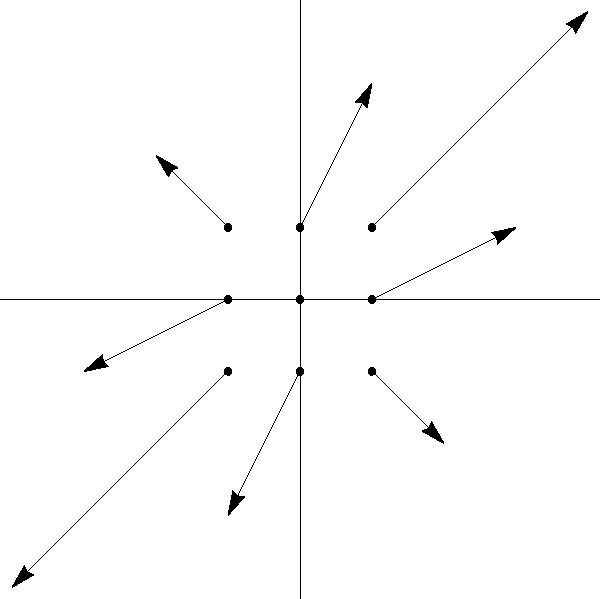
\includegraphics[height=2in]{02-Applications/support/vf21128points}};
\end{tikzpicture}
\end{center}


Notice that (1,1) is an eigenvector corresponding to the eigenvalue 3 because $A(1,1) = 3(1,1)$. 
Also, note that $(-1,1)$ is an eigenvector corresponding to the eigenvalue 1 because $A(-1,1)=(-1,1)$. 
These two eigenvectors represent the directions in which the vector field pushes objects radially outwards.   \marginpar{Eigenvectors tell you where vector fields push radially outwards or inwards.  Eigenvalues tell the strength and direction (outward or inward) of the push.}%
Anywhere along the line spanned by an eigenvector, the vector field pushes radially outward (as shown in the middle figure).  The vector field will never push you from one side of an eigenvector to the other side.
The eigenvalue for the eigenvector tells you the strength of the push, which explains why the vectors in the $(1,1)$ direction are three times as long as the vectors in the $(-1,1)$ direction. 
The middle plot in Figure \ref{vf2112} includes two lines representing the eigenvector directions.

\begin{figure}[bth]
\begin{tikzpicture}[inner sep=0mm]
\node (A) 
{
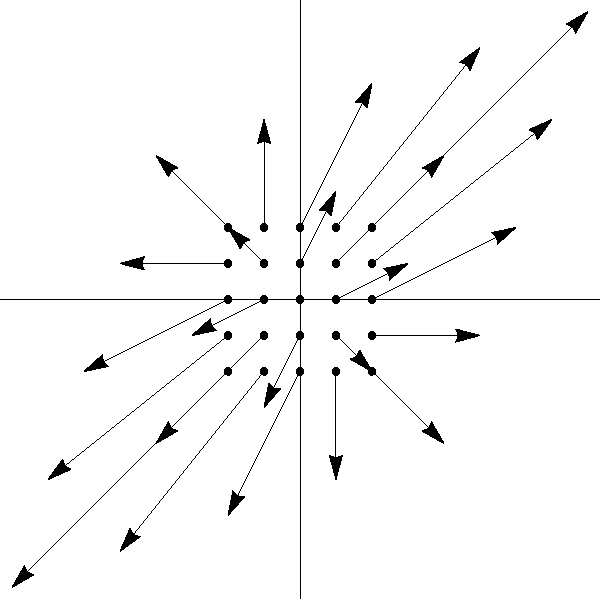
\includegraphics[height=1.3in]{02-Applications/support/vf211225points}
};
\node (B) [right=of A] 
{
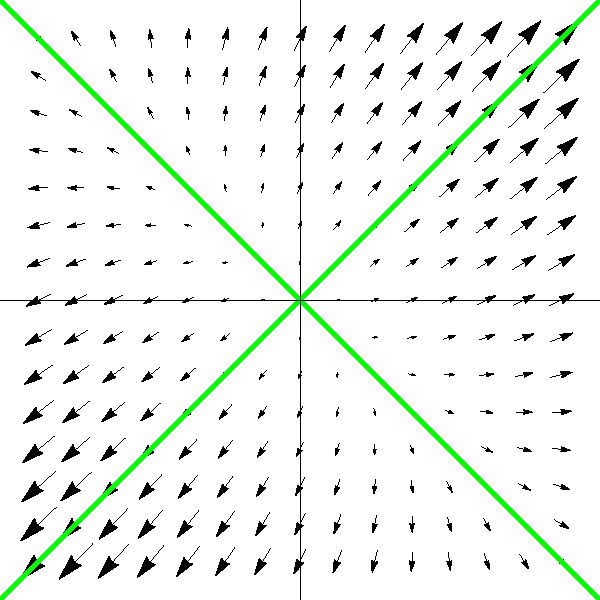
\includegraphics[height=1.3in]{02-Applications/support/vf2112com}
};
\node (C) [right=of B] 
{
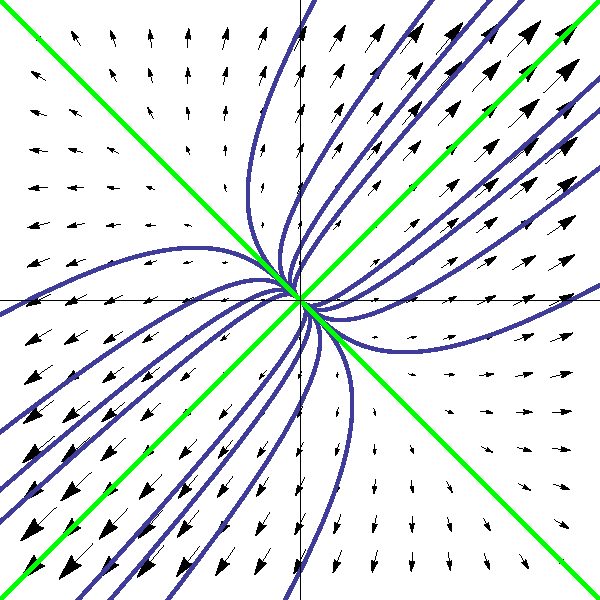
\includegraphics[height=1.3in]{02-Applications/support/vf2112flow}
};
\end{tikzpicture}
\caption{\label{vf2112} Three views of the vector field $\vec F(x,y) =(2x+y,x+2y)$. The first plot shows the appropriate lengths.  The second plot includes two lines which come from the eigenvector directions. The third plot includes flow lines which describe the path of an object flowing through the vector field. Because flow is outward in all directions, this vector field is called a source.}
\end{figure}

When a computer draws a vector field, it creates hundreds of vectors, takes the longest vector and shrinks its length so that it won't cross any others, and then proportionally shrinks every other vector. This creates lots of tiny vectors which represent the directions (not magnitudes) of the vectors (see the last two plots in Figure \ref{vf2112}). You can think of a vector field as the flow of water---if you were to drop a particle into the field, then it would follow the vectors (just as drift wood follows the flow of a river). These flow lines are represented in the last plot of Figure \ref{vf2112}.
\end{example} 

Figure \ref{vflots} contains other examples. Again, the eigenvalues and eigenvectors determine how to draw flow lines in the graph.

\begin{figure}
\begin{tikzpicture}[inner sep=0mm]
\node (B0) 
{
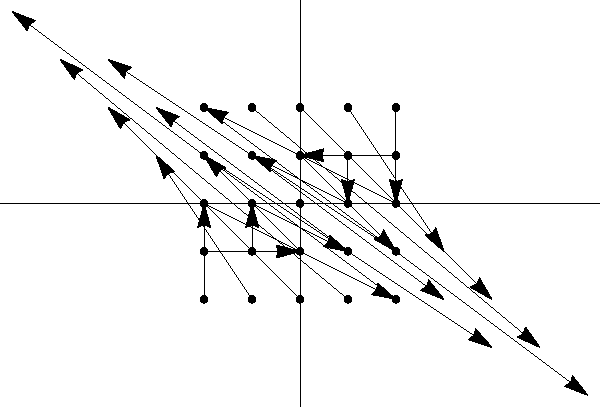
\includegraphics[width=1.3in]{02-Applications/support/vfsinkhand}
};
\node (A0) [left=of B0] 
{
\begin{tabular}{c}
Sink (inward flow)
\\ \hline
$A=
\begin{bmatrix}
 -2 & 2 \\
 1 & -2
\end{bmatrix}
$
\\
Eigenvalues: $-2-\sqrt{2},\sqrt{2}-2$
\\
Eigenvectors: $(-\sqrt{2} ,1), (\sqrt{2}, 1)$
\end{tabular}
};
\node (C0) [right=of B0] 
{
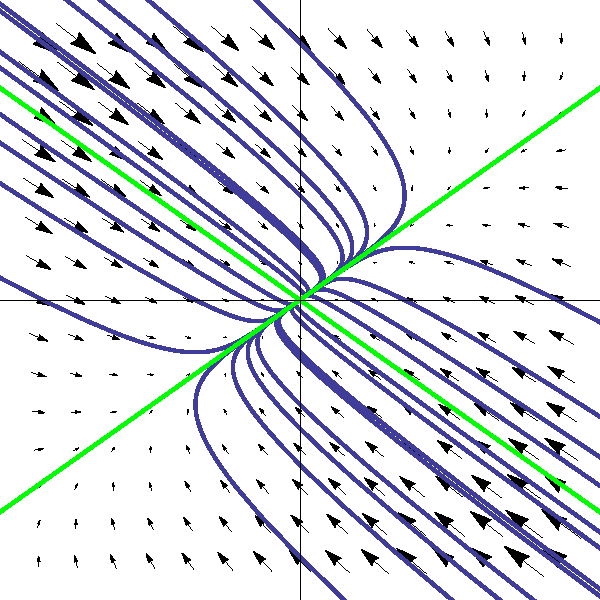
\includegraphics[width=1.3in]{02-Applications/support/vfsinkcom}
};

\node (B1) [below=of B0]
{
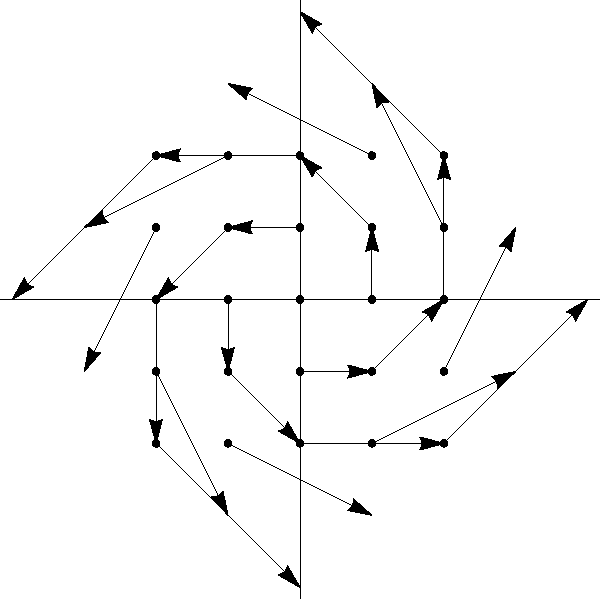
\includegraphics[width=1.3in]{02-Applications/support/vfrotationalhand}
};
\node (A1) [left=of B1] 
{
\begin{tabular}{c}
Rotational
\\ \hline
$A=
\begin{bmatrix}
 0 & -1 \\
 1 & 0
\end{bmatrix}
$
\\
Eigenvalues: $i,-i$
\\
Eigenvectors: $(i,1), (-1, 1)$
\end{tabular}
};
\node (C1) [right=of B1] 
{
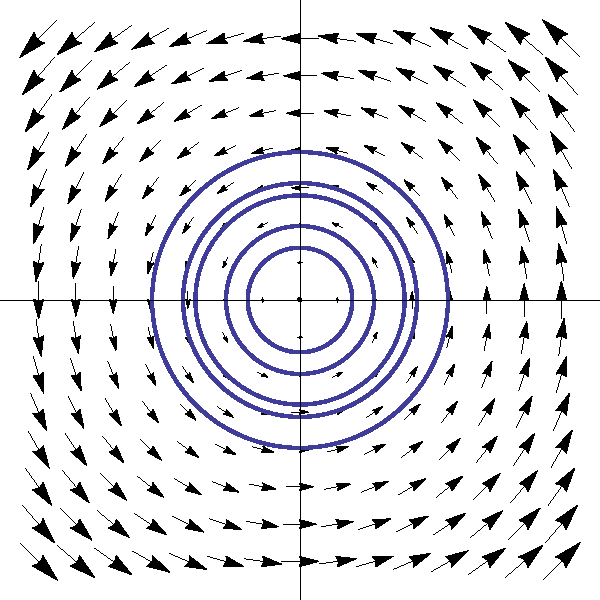
\includegraphics[width=1.3in]{02-Applications/support/vfrotationalcom}
};

\node (B2) [below=of B1] 
{
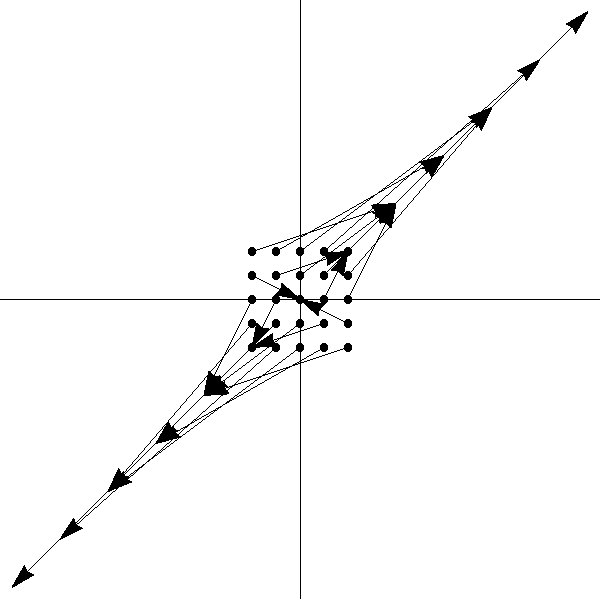
\includegraphics[width=1.3in]{02-Applications/support/vfsaddlehand}
};
\node (A2) [left=of B2]
{
\begin{tabular}{c}
Saddle (both in and out)
\\ \hline
$A=
\begin{bmatrix}
 -1 & 4 \\
 2 & 3
\end{bmatrix}
$
\\
Eigenvalues: $5,-1$
\\
Eigenvectors: $(1,1), (-2, 1)$
\end{tabular}
};
\node (C2) [right=of B2] 
{
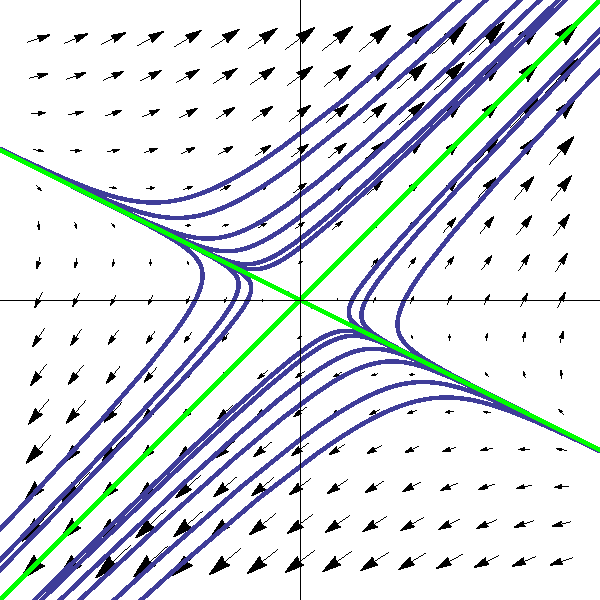
\includegraphics[width=1.3in]{02-Applications/support/vfsaddlecom}
};

\node (B3) [below=of B2] 
{
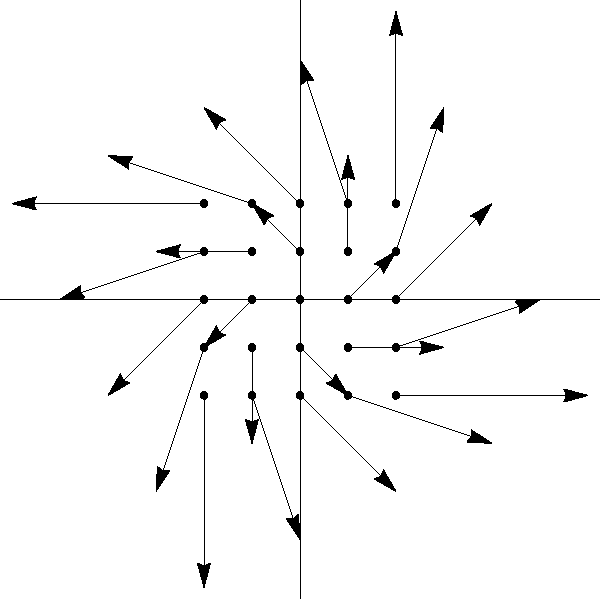
\includegraphics[width=1.3in]{02-Applications/support/vfspiralhand}
};
\node (A3) [left=of B3]
{
\begin{tabular}{c}
Outward Spiral
\\ \hline
$A=
\begin{bmatrix}
 1 & -1 \\
 1 & 1
\end{bmatrix}
$
\\
Eigenvalues: $1+i, 1-i$
\\
Eigenvectors: $(i ,1), (-i, 1)$
\end{tabular}
};
\node (C3) [right=of B3] 
{
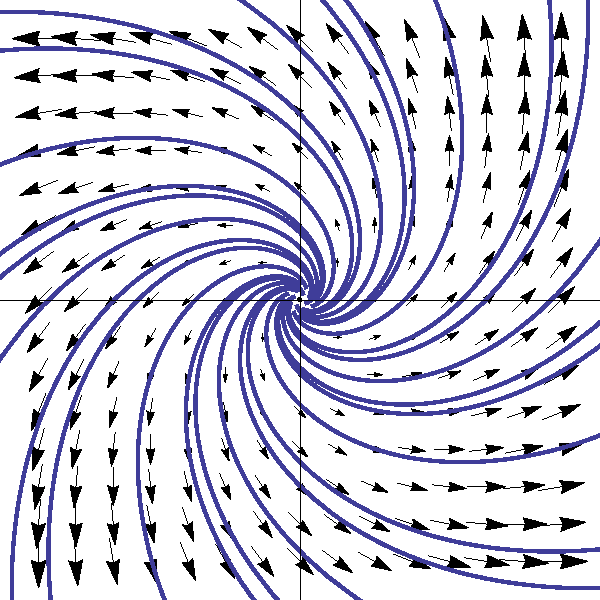
\includegraphics[width=1.3in]{02-Applications/support/vfspiralcom}
};




\end{tikzpicture}
\caption{\label{vflots}
Different kinds of vector fields.  Every 2 by 2 matrix represents a vector field.  When the eigenvalues are real, the eigenvectors help determine direction of flow. Positive eigenvalues result in outward flow along the corresponding eigenvector. Negative eigenvalues result in inward flow. Pure imaginary eigenvalues yield rotational flow. When the eigenvalues involve both real and imaginary parts, the real part determines whether the flow is inward or outward, and the complex part determines rotation.
}
\end{figure}











\section{The Second Derivative Test}

In this section, we'll explore how eigenvalues and eigenvectors of a matrix are the key tool needed to generalize the second derivative test from first semester calculus to all dimensions. The key application is that eigenvalues tell you about concavity of a function in the eigenvector directions.  If all eigenvalues are negative, then a function is concave downwards in all directions, which means that a critical point must correspond to a maximum.    

Let's start with a review from first semester calculus. 
If a function $y=f(x)$ has a relative extreme value at $x=c$, then $f^\prime(c)=0$ or the derivative is undefined. 
The places where the derivative is either zero or undefined are called critical values of the function. 
The first derivative test allows you to check the value of the derivative on both sides of the critical value and then interpret whether that point is a maximum or minimum using increasing/decreasing arguments.  
The second derivative test requires you to compute the second derivative at $x=c$ and then make an observation. 
If $f''(c)>0$ (the function is concave upwards), then the function has a minimum at $x=c$. 
If $f''(c)<0$ (the function is concave downwards), then the function has a maximum at $x=c$. 
If $f''(c)=0$, then the second derivative test fails. 
\note{pictures would be good}

\begin{example}
The function $f(x) = x^3-3x$ has derivatives $f^\prime = 3x^2-3$ and $f^{\prime\prime}=6x$.  The first derivative is zero when $3(x^2-1)=3(x-1)(x+1)=0$, or $x=\pm 1$.  
The second derivative at $x=1$ is $f''(1)=6$ (concave upwards), so there is a minimum at $x=1$.  
The second derivative at $x=-1$ is $f''(-1)=-6$ (concave downwards),
so there is a maximum at that point. This is all illustrated in the margin.
\marginpar{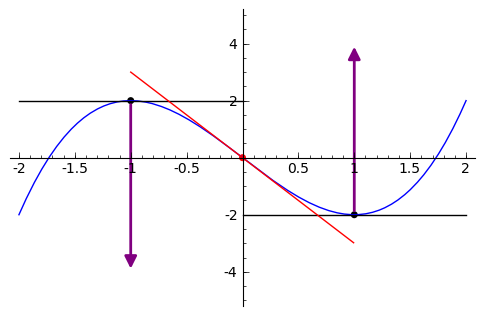
\includegraphics[width=\marginparwidth]{02-Applications/support/sage0.png}}
\end{example}

\subsection{Partial Derivatives}

Before extending the second derivative test to all dimensions, we have to talk about taking derivatives.
If a function has more than one input variable, say $f(x,y)=9-x^2+3y$ which has 2 input variables, then we have to take multiple derivatives, one with respect to each variable.  
These derivatives (called partial derivatives) are found by holding all variables constant except the one you want the derivative with respect to, and then just computing a normal derivative.
For the function $f(x,y)$, we define the partial derivative of $f$ with respect to $x$ as 
$$\ds f_x(x,y)=f_x = \frac{\partial f}{\partial x}= \lim_{h\to 0}\frac{f(x+h,y)-f(x,y)}{h},$$
and the partial derivative of $f$ with respect to $y$ as 
$$\ds f_y(x,y)=f_y =\frac{\partial f}{\partial y}= \lim_{k\to 0}\frac{f(x,y+k)-f(x,y)}{k}.$$
Notice that $f_x$ computes a limit as $y$ is held constant and we vary $x$. 

\begin{example}
For $f(x,y)=3x^2+4xy+\cos(xy)+y^3$, we obtain $f_x=6x+4y-y\sin(xy)+0$ and $f_y=0+4x-x\sin(xy)+3y^2$. 
Partial derivatives are found by holding all other variables constant, and then differentiating with respect to the variable in question.
\end{example}

\subsection{The Derivative}
The derivative of a function $\vec f\colon\RR^n\to\RR^m$
is an $m\times n$ matrix written $D\vec f(\vec x)$, where the columns
of the matrix are the partial derivatives of the function with respect
to an input variable (the first column is the partial derivative with
respect to the first variable, and so on). Some people call this
derivative the ``total'' derivative instead of the derivative, to
emphasize that the ``total'' derivative combines the ``partial''
derivatives into a matrix. Some examples of functions and their
derivative are in Table \ref{dertable}. Remember that each column of
the matrix corresponds to the partial derivatives with respect to an input variable.
\begin{table}[htb]
\begin{center}
\begin{tabular}{|l|l|}
\hline
Function&Derivative\\ \hline
{$f(x)=x^2$}& {$Df(x) = \begin{bmatrix}2x\end{bmatrix} $}\\ \hline
{$\vec r(t) = \left<3\cos(t),2\sin(t)\right>$}&  {$D\vec r(t) = \begin{bmatrix}-3\sin t\\ 2\cos t\end{bmatrix} $}\\ \hline
{$\vec r(t) = \left<\cos(t),\sin(t),t\right>$}&  {$D\vec r(t) = \begin{bmatrix}-\sin t \\ \cos t \\ 1\end{bmatrix} $}\\ \hline
{$f(x,y)=9-x^2-y^2$}&  {$Df(x,y) = \begin{bmatrix}-2x & -2y\end{bmatrix} $}\\ \hline
{$f(x,y,z)=x^2+y+xz^2$}&  {$Df(x,y,z) = \begin{bmatrix}2x+z^2 & 1 &2xz\end{bmatrix} $}\\ \hline
{$\vec F(x,y)=\left<-y,x\right>$}&  {$D\vec F(x,y) = \begin{bmatrix}0&-1\\ 1&0\end{bmatrix} $}\\ \hline
{$\vec F(r,\theta,z)=\left<r\cos\theta,r\sin\theta,z\right>$}&  {$D\vec F(r,\theta,z) = 
\begin{bmatrix}
\cos \theta &-r\sin\theta&0\\ 
\sin\theta&r\cos\theta&0\\ 
0&0&1
\end{bmatrix} $}\\ \hline
{$\vec r (u,v)=\left<u,v,9-u^2-v^2\right>$}&  {$D\vec r(u,v) = \begin{bmatrix}1&0\\ 0&1\\ -2u&-2v\end{bmatrix} $}\\ \hline
\end{tabular}
\end{center}
\caption{\label{dertable} Derivatives of functions are found by creating a matrix whose columns are the partial derivatives of the function.  If the function has multiple outputs, then the columns of the matrix will have one row for each output.  Hence a function with 2 inputs and 3 outputs will have 2 columns with 3 rows in each column.}
\end{table}

\subsection{The Second Derivative Test}
We're now ready to extend the second derivative test to all dimensions. We'll focus on only functions of the form $f\colon{\RR}^2\to{\RR}$, as this gives you the tools needed to study optimization in all dimensions. Because the output is one-dimensional, it makes sense to talk about a largest or smallest number.

The first derivative test does not work when the domain has more than one dimension because there are infinitely many ways to approach a point---you can't just look at the left and right side to decide if you are at an optimum value. 
However, at a local extreme value the derivative is still zero, which results in solving a system of equations to find any critical points. 
In higher dimensions, there are three classifications of critical points: maximum, minimum, or saddle point (a point where the tangent plane is horizontal, but in some directions you increase and in other directions you decrease). 

The second derivative test does work when the domain has dimension greater than one. Consider the function $z=f(x,y)$. 
Its derivative $Df(x,y) = \begin{bmatrix}f_x&f_y\end{bmatrix}$ is a function with two inputs $(x,y)$ and two outputs $(f_x,f_y)$. 
The second derivative {$D^2f (x,y)= \begin{bmatrix}f_{xx}&f_{xy}\\f_{yx}&f_{yy}\end{bmatrix} $} is a {$2\times 2$} square matrix called the Hessian of $f$. 
This matrix will always be symmetric, in that the transpose of the matrix equals itself (because $f_{xy}=f_{yx}$ from a theorem in multivariable calculus).  
At a critical point (where the first derivative is zero), the eigenvalues of $D^2f$ give the directional second derivative in the direction of a corresponding eigenvector. 
The largest eigenvalue is the largest possible value of the second derivative in any direction and the smallest eigenvalue is the smallest possible value of the second derivative in any direction. 

\marginpar{the second derivative test with eigenvalues}%
The \textbf{second derivative test} is the following. Start by finding all the critical points (places where the derivative is zero). Then find the eigenvalues of the second derivative. Each eigenvalue represents the directional 2nd derivative in the direction of a corresponding eigenvector. In every other direction, the directional 2nd derivative is between the smallest and largest eigenvalue.  
\begin{enumerate}
	\item If the eigenvalues are all positive at a critical point, then in every direction the function is concave upwards. The function has a minimum at that critical point.
	\item If the eigenvalues are all negative at a critical point, then in every direction the function is concave downwards. The function has a maximum there.
	\item If there is a positive eigenvalue and a negative eigenvalue, the function has a saddle point there.  
	\item If either the largest or smallest eigenvalue is zero, then the second derivative test fails. 
\end{enumerate}
Eigenvalues are the key numbers needed to generalize optimization to all dimensions. A proof of this fact is beyond the scope of this class. 

\begin{example}
For the function {$f(x,y)=x^2+xy+y^2$}, the derivative is $Df = \begin{bmatrix}2x+y&x+2y \end{bmatrix}$, which is zero only at $x=0,y=0$ (solve the system of equations $2x+y=0,x+2y=0$). 
\marginpar{The Hessian ($D^2f$) is always symmetric.}
The Hessian is $D^2f = \begin{bmatrix}2&1 \\1&2\end{bmatrix}$. The eigenvalues are found by solving $0=\det \begin{bmatrix}2-\lambda &1 \\1&2-\lambda \end{bmatrix} = (2-\lambda)^2-1 = 4-4\lambda+\lambda^2 -1 = (\lambda-3)(\lambda-1)$, so $\lambda = 3,1$ are the eigenvalues.  Since both eigenvalues are positive, the function is concave upwards in all directions, so there is a minimum at $(0,0)$.  

The eigenvectors of the Hessian help us understand more about the graph of the function.  An eigenvector corresponding to 3 is $(1,1)$, and corresponding to 1 is $(-1,1)$. These vectors are drawn in the graph of the function in the margin, together with two parabolas whose 2nd derivatives are precisely 3 and 1.  The parabola which opens upwards the most quickly has a 2nd derivative of 3.  The other parabola has a second derivative of 1. In every other direction, the 2nd derivative would be between 1 and 3.
\marginpar{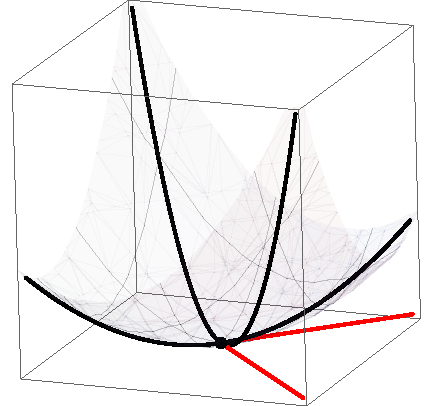
\includegraphics[width=\marginparwidth]{02-Applications/support/2nddertest1}}
\end{example}

\begin{example}
For the function {$f(x,y)=x^3-3x+y^2-4y$}, the derivative is $Df = \begin{bmatrix}3x^2-3&2y-4 \end{bmatrix}$, which is zero at $x=1,y=2$ or $x=-1,y=2$. Hence there are two critical points, so we have to find two sets of eigenvalues. The Hessian is $D^2f = \begin{bmatrix}6x&0 \\0&2\end{bmatrix}$. When $x=-1,y=2$, the eigenvalues of $\begin{bmatrix}-6&0 \\0&2\end{bmatrix}$ are $\lambda=-6,2$. Since one is positive and one is negative, there is a saddle point at $(-1,2)$. When $x=1,y=2$, the eigenvalues of $\begin{bmatrix}6&0 \\0&2\end{bmatrix}$ are $\lambda=6,2$. Since both are positive, there is a minimum at $(-1,2)$ (as in every direction the function is concave upwards).

Again the eigenvectors help us understand how the function behaves, as illustrated in the margin.  At $(1,2)$, we have an eigenvector $(1,0)$ corresponding to 6, and $(0,1)$ corresponding to 2. In both eigenvector directions, the function is concave upwards, but opens more steeply in the $(1,0)$ direction since \mbox{$6>2$}.  At $(-1,2)$, we have an eigenvector $(1,0)$ corresponding to $-6$, and $(0,1)$ corresponding to 2. The functions opens steeply downwards in the $(1,0)$ direction, and upwards in the $(0,1)$ direction.
\marginpar{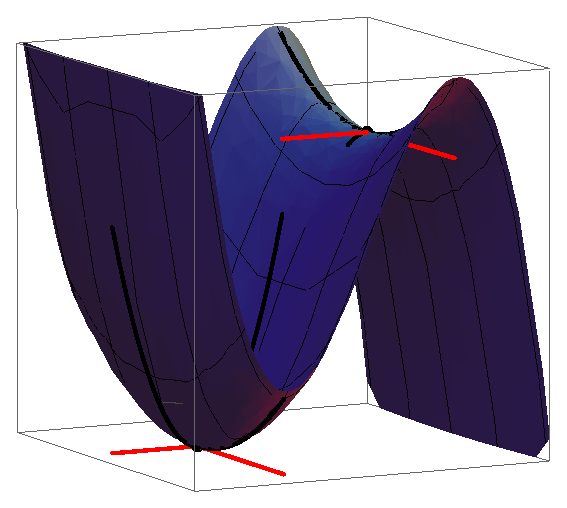
\includegraphics[width=\marginparwidth]{02-Applications/support/2nddertest2}}
\end{example}















\section{Markov Processes}

Matrices can be used to model a process called a Markov process. To fit this kind of model, a process must have specific states, and the matrix which models the process is a transition matrix which specifies how each state will change through a given transition. An example of a set of states is ``open'' or ``closed'' in an electrical circuit, or ``working properly'' and ``working improperly'' for operation of machinery at a manufacturing facility. A car rental company which rents vehicles in different locations can use a Markov Process to keep track of where their inventory of cars will be in the future. Stock market analysts use Markov processes and generalizations, liked stochastic processes and hidden Markov models, to make predictions about future stock values.  The algorithm that powers Google's internet search is based on the idea that browsing the web is a Markov process.

\begin{example} Let's illustrate a Markov Process related to classifying land in some region as ``Residential,'' ``Commercial,'' or ``Industrial.'' Suppose in a given region over a 5 year time span that 80\% of residential land will remain residential, 10\% becomes commercial, and 10\%  becomes industrial. For commerical land, 70\% remains commercial, 20\% becomes residential, and 10\% becomes industrial.  For industrial land, 70\% remains industrial, 30\% becomes commercial, and 0\% becomes residential.  To predict what happens to the land zoning at the end of a 5 year period, provided we know the current $R$, $C$, and $I$ values, we would compute \marginpar{Notice that the percentages go in columns. The residential percentages $(.8,.1,.1)$ become the first column. This gives us the transistion matrix
$$ \begin{array}{rl}
&\begin{array}{ccc} R&C&I \end{array} \\
 \begin{array}{c} \text{to }R\\ \text{to }C\\ \text{to }I \end{array}& 
\begin {bmatrix}  .8&.2&0\\.1&.7&.3\\.1&.1&.7 \end {bmatrix} \\
\multicolumn{2}{c}{\text{Transition Matrix}}
\end{array}.
$$ 
}
$$
\begin{array}{rl}
R_{\text{new}} &= .8 R+ .2 C+0 I\\ 
C_{\text{new}} &= .1 R+ .7 C+.3 I\\ 
I_{\text{new}} &= .1 R+ .1 C+.7 I 
\end{array}
\xrightarrow{\text{matrix form}}
\begin{bmatrix}
R_{\text{new}}\\ 
C_{\text{new}}\\ 
I_{\text{new}} 
\end{bmatrix}
=
\begin{bmatrix}
.8& .2 &0 \\ 
.1& .7 &.3\\ 
.1& .1 &.7 
\end{bmatrix}
\begin{bmatrix}
R\\ 
C\\ 
I 
\end{bmatrix}
$$
The matrix on the right above is called the transition matrix of the Markov process. 
It is a matrix where each column relates to one of the ``states,'' and the numbers in that column are the proportions of the column state that will change to the row state through the transition (the ordering on row and column states is the same). 
We calculate the next ``state'' by multiplying our current state by the transition matrix. If current land use is about 50\% residential, 30\% commercial, and 20\% industrial, then 5 years later the land use would be 
$$ 
A\vec x= \begin {bmatrix} .8&.2&0\\.1&.7&.3\\.1&.1&.7 \end {bmatrix}
 \begin {bmatrix} 50\\30\\20 \end {bmatrix}
 =   \begin {bmatrix} 46\\ 32 \\ 22\end {bmatrix}
$$  If the same transitions in land use continue, we can multiply the previous projection (state) by the transition matrix to obtain a 10 and 15 year projection for land use:  
\begin{center}\begin{tabular}{cc}
$A(A \vec x) =A^2 \vec x$&$A(A^2\vec x)=A^3\vec x$\\
$
\begin {bmatrix} .8&.2&0\\.1&.7&.3\\.1&.1&.7 \end {bmatrix}
\begin {bmatrix} 46\\ 32 \\ 22 \end {bmatrix}
 =   \begin {bmatrix} 43.2\\ 33.6 \\ 23.2\end {bmatrix}
$ 
&
$
\begin {bmatrix} .8&.2&0\\.1&.7&.3\\.1&.1&.7 \end {bmatrix}
\begin {bmatrix} 43.2\\ 33.6 \\ 23.2 \end {bmatrix}
 =   \begin {bmatrix} 41.28\\ 34.8\\ 23.92\end {bmatrix}
$ 
\\
10 Year Projection 
&15 Year Projection 
\end{tabular}\end{center}
Each time we multiply on the left by our transition matrix, we add 5 more years to our projection. This projection is valid as long as the same trends continue. 
\end{example}










\subsection{Steady State Solutions}


Consider the land use example from above.  Let $\vec x_0$ be our initial state. If our transition matrix $A$ remains the same forever, what will eventually be the proportion of land devoted to residential, commercial, or industrial use? We can write each new state as powers of the transition matrix $A$ by writing 
$$\vec x_{1} = A \vec x_{0}, \quad \vec x_{2}=A \vec x_{1} = AA\vec x_{0} = A^2\vec x_{0},\quad \vec x_{3}= A^3\vec x_{0},\quad \vec x_{n}= A^n\vec x_{0}.$$  What happens to the product $A^n\vec x_0$ as $n\to \infty$? Can we reach a state $\vec x = (R,C,I)$ such that $A \vec x=\vec x$, where the next state is the same as the current? If this occurs, then any future transitions will not change the state either. This state $\vec x$ is called a \emph{steady state}, since it does not change when multiplied by the transition matrix (it remains steady). 

Let's look more closely at the steady state equation $$A\vec x = \vec x = 1\vec x.$$ 
Do you see the eigenvalue-eigenvector notation $A\vec x = \lambda \vec x$? 
\marginpar{The number $\lambda =1$ is always an eigenvalue of the transition matrix.  Steady states are eigenvectors of the transition matrix.}
The eigenvalue is 1 and the steady state is an eigenvector. 
Without even thinking that an eigenvalue was important, we reduced finding a steady state to an eigenvalue-eigenvector problem. 
For any Markov process (the columns of the matrix must sum to 1), the number $\lambda = 1$ will always be an eigenvalue. All we have to do is find the eigenvectors corresponding to the eigenvalue 1. 
The solution to $\ds\lim_{n\to\infty}A^n \vec x_0$ is this steady state, and is an eigenvector of the transition matrix.
 
\begin{example}
For the land use Markov process from the previous example, an eigenvector corresponding to 1 is $\left(\frac{3}{2},\frac32,1\right)$. 
Since any nonzero multiple of an eigenvector is again an eigenvector, we can multiply by a constant so that the proportions sum to 100. 
Multiplying by 2 we have $(3,3,2)$, which means that the ratio of land will be 3 acres residential to 3 acres commercial to 2 acres industrial. 
\marginpar{Divide each entry by the sum to get percentages.}
To write this in terms of percentages, divide each component by 8 (the sum $3+3+2$) to obtain $3/8:3/8:2/8$. Multiply by 100 to get the percentages $37.5\%:37.5\%:25\%$, the long term percentages of land use.
\end{example}


















\section{Kirchoff's Electrial Laws}
Gustav Kirchoff discovered two laws of electricity that pertain to the conservation of charge and energy. 
%In short, his two laws state that current in equals current out, and volts in equals volts out. 
To fully describe these laws, we must first discuss voltage, resistance, and current.  
Current is the flow of electricity; often you can compare it to the flow of water.  As a current passes across a conductor, it encounters resistance. 
Ohm's law states that the product of the resistance $R$ and current $I$ across a conductor equals a drop in voltage $V$, i.e. $RI=V$. \marginpar{\begin{center}Ohm's law: \\ Voltage = Resistance $\times$ Current$$V=RI$$\end{center}}
If the voltage remains constant, then a large resistance corresponds to a small current. 
A resistor is an object with high resistance which is placed in an electrical system to slow down the flow (current) of electricity. 
Resistors are measured in terms of ohms, and the larger the ohms, the smaller the current.  Figure \ref{ecir} illustrates two introductory electrical systems. 



\begin{figure}[htb]
\begin{center}
\begin{tabular}{cc}
\renewcommand{\myscale}{.3}
\begin{tikzpicture}[scale=\myscale,inner sep=1pt]
%\draw[help lines,step=1cm] (0,0) grid (12,6);

%Source - like a battery
\node[label=right:$E$] at (0,3) 
{{\begin{tikzpicture}[scale=\myscale]
%	\useasboundingbox (-.5,-3) rectangle (.5,3);
	\draw (0,0) circle (1cm);
	\draw (.3,.5) -- (-.3,.5);
	\draw (0,.2) -- (0,.8);
	\draw (.3,-.5) -- (-.3,-.5);
	\draw (0,1) -- (0,3);
	\draw (0,-1) -- (0,-3);
	\end{tikzpicture}
}};

%Resistor
\node[label=right:$R_2$] at (6,3) 
{{\begin{tikzpicture}[scale=\myscale]
%	\useasboundingbox (0,-3) rectangle (0,3);
	\draw (0,-3) -- ++(0,1.8) -- ++(.5,.2) 
		-- ++(-1,.4) -- ++(1,.4)
		-- ++(-1,.4) -- ++(1,.4)
		-- ++(-1,.4) -- ++(.5,.2)
		-- ++(0,1.8) ;
	\end{tikzpicture}
}};

%Resistor
\node[label=above:$R_1$] at (3,0) 
{{\begin{tikzpicture}[scale=\myscale,rotate=90]
%	\useasboundingbox (0,-3) rectangle (0,3);
	\draw (0,-3) -- ++(0,1.8) -- ++(.5,.2) 
		-- ++(-1,.4) -- ++(1,.4)
		-- ++(-1,.4) -- ++(1,.4)
		-- ++(-1,.4) -- ++(.5,.2)
		-- ++(0,1.8) ;
	\end{tikzpicture}
}};

%Resistor
\node[label=right:$R_3$] at (12,3) 
{{\begin{tikzpicture}[scale=\myscale,rotate=0]
%	\useasboundingbox (0,-3) rectangle (0,3);
	\draw (0,-3) -- ++(0,1.8) -- ++(.5,.2) 
		-- ++(-1,.4) -- ++(1,.4)
		-- ++(-1,.4) -- ++(1,.4)
		-- ++(-1,.4) -- ++(.5,.2)
		-- ++(0,1.8) ;
	\end{tikzpicture}
}};

%Straight Path
\node at (3,6) 
{{\begin{tikzpicture}[scale=\myscale,rotate=90]
	\draw (0,-3) -- (0,3);
	\end{tikzpicture}
}};

%Straight Path
\node at (9,6) 
{{\begin{tikzpicture}[scale=\myscale,rotate=90]
	\draw (0,-3) -- (0,3);
	\end{tikzpicture}
}};

%Straight Path
\node at (9,0) 
{{\begin{tikzpicture}[scale=\myscale,rotate=90]
	\draw (0,-3) -- (0,3);
	\end{tikzpicture}
}};


%Arrow to represent Current
\node[label=above:$i_1$] at (3,6) 
{{\begin{tikzpicture}[scale=\myscale,rotate=-90]
%	\useasboundingbox (0,-.4) rectangle (0,.4);
	\filldraw (0,.4) -- (-.2,-.4) -- (0,-.3) -- (.2,-.4);
	\end{tikzpicture}
}};

%Arrow to represent Current
\node[label=right:$i_2$] at (6,5) 
{{\begin{tikzpicture}[scale=\myscale,rotate=180]
%	\useasboundingbox (0,-.4) rectangle (0,.4);
	\filldraw (0,.4) -- (-.2,-.4) -- (0,-.3) -- (.2,-.4);
	\end{tikzpicture}
}};

%Arrow to represent Current
\node[label=above:$i_3$] at (9,6) 
{{\begin{tikzpicture}[scale=\myscale,rotate=-90]
%	\useasboundingbox (0,-.4) rectangle (0,.4);
	\filldraw (0,.4) -- (-.2,-.4) -- (0,-.3) -- (.2,-.4);
	\end{tikzpicture}
}};

%Node
\node at (6,6) 
{{\begin{tikzpicture}[scale=\myscale,rotate=-90]
%	\useasboundingbox (0,-.4) rectangle (0,.4);
	\filldraw (0,0) circle (.15cm);
	\end{tikzpicture}
}};

%Node
\node at (6,0) 
{{\begin{tikzpicture}[scale=\myscale,rotate=-90]
%	\useasboundingbox (0,-.4) rectangle (0,.4);
	\filldraw (0,0) circle (.15cm);
	\end{tikzpicture}
}};

\end{tikzpicture}

&
\renewcommand{\myscale}{.3}
\begin{tikzpicture}[scale=\myscale,inner sep=1pt]
%\draw[help lines,step=1cm] (0,0) grid (18,6);

%Source - like a battery
\node[label=right:$E$] at (0,3) 
{{\begin{tikzpicture}[scale=\myscale]
%	\useasboundingbox (-.5,-3) rectangle (.5,3);
	\draw (0,0) circle (1cm);
	\draw (.3,.5) -- (-.3,.5);
	\draw (0,.2) -- (0,.8);
	\draw (.3,-.5) -- (-.3,-.5);
	\draw (0,1) -- (0,3);
	\draw (0,-1) -- (0,-3);
	\end{tikzpicture}
}};

%Resistor
\node[label=right:$R_2$] at (6,3) 
{{\begin{tikzpicture}[scale=\myscale]
%	\useasboundingbox (0,-3) rectangle (0,3);
	\draw (0,-3) -- ++(0,1.8) -- ++(.5,.2) 
		-- ++(-1,.4) -- ++(1,.4)
		-- ++(-1,.4) -- ++(1,.4)
		-- ++(-1,.4) -- ++(.5,.2)
		-- ++(0,1.8) ;
	\end{tikzpicture}
}};

%Resistor
\node[label=above:$R_1$] at (3,0) 
{{\begin{tikzpicture}[scale=\myscale,rotate=90]
%	\useasboundingbox (0,-3) rectangle (0,3);
	\draw (0,-3) -- ++(0,1.8) -- ++(.5,.2) 
		-- ++(-1,.4) -- ++(1,.4)
		-- ++(-1,.4) -- ++(1,.4)
		-- ++(-1,.4) -- ++(.5,.2)
		-- ++(0,1.8) ;
	\end{tikzpicture}
}};

%Resistor
\node[label=above:$R_3$] at (9,6) 
{{\begin{tikzpicture}[scale=\myscale,rotate=90]
%	\useasboundingbox (0,-3) rectangle (0,3);
	\draw (0,-3) -- ++(0,1.8) -- ++(.5,.2) 
		-- ++(-1,.4) -- ++(1,.4)
		-- ++(-1,.4) -- ++(1,.4)
		-- ++(-1,.4) -- ++(.5,.2)
		-- ++(0,1.8) ;
	\end{tikzpicture}
}};

%Resistor
\node[label=right:$R_4$] at (12,3) 
{{\begin{tikzpicture}[scale=\myscale,rotate=0]
%	\useasboundingbox (0,-3) rectangle (0,3);
	\draw (0,-3) -- ++(0,1.8) -- ++(.5,.2) 
		-- ++(-1,.4) -- ++(1,.4)
		-- ++(-1,.4) -- ++(1,.4)
		-- ++(-1,.4) -- ++(.5,.2)
		-- ++(0,1.8) ;
	\end{tikzpicture}
}};

%Resistor
\node[label=right:$R_5$] at (18,3) 
{{\begin{tikzpicture}[scale=\myscale,rotate=0]
%	\useasboundingbox (0,-3) rectangle (0,3);
	\draw (0,-3) -- ++(0,1.8) -- ++(.5,.2) 
		-- ++(-1,.4) -- ++(1,.4)
		-- ++(-1,.4) -- ++(1,.4)
		-- ++(-1,.4) -- ++(.5,.2)
		-- ++(0,1.8) ;
	\end{tikzpicture}
}};

%Resistor
\node[label=above:$R_6$] at (9,0) 
{{\begin{tikzpicture}[scale=\myscale,rotate=90]
%	\useasboundingbox (0,-3) rectangle (0,3);
	\draw (0,-3) -- ++(0,1.8) -- ++(.5,.2) 
		-- ++(-1,.4) -- ++(1,.4)
		-- ++(-1,.4) -- ++(1,.4)
		-- ++(-1,.4) -- ++(.5,.2)
		-- ++(0,1.8) ;
	\end{tikzpicture}
}};









%Straight Path
\node at (3,6) 
{{\begin{tikzpicture}[scale=\myscale,rotate=90]
	\draw (0,-3) -- (0,3);
	\end{tikzpicture}
}};

%Straight Path
\node at (15,6) 
{{\begin{tikzpicture}[scale=\myscale,rotate=90]
	\draw (0,-3) -- (0,3);
	\end{tikzpicture}
}};

%Straight Path
\node at (15,0) 
{{\begin{tikzpicture}[scale=\myscale,rotate=90]
	\draw (0,-3) -- (0,3);
	\end{tikzpicture}
}};






%Arrow to represent Current
\node[label=above:$i_1$] at (3,6) 
{{\begin{tikzpicture}[scale=\myscale,rotate=-90]
%	\useasboundingbox (0,-.4) rectangle (0,.4);
	\filldraw (0,.4) -- (-.2,-.4) -- (0,-.3) -- (.2,-.4);
	\end{tikzpicture}
}};

%Arrow to represent Current
\node[label=right:$i_2$] at (6,5) 
{{\begin{tikzpicture}[scale=\myscale,rotate=180]
%	\useasboundingbox (0,-.4) rectangle (0,.4);
	\filldraw (0,.4) -- (-.2,-.4) -- (0,-.3) -- (.2,-.4);
	\end{tikzpicture}
}};

%Arrow to represent Current
\node[label=above:$i_3$] at (7,6) 
{{\begin{tikzpicture}[scale=\myscale,rotate=-90]
%	\useasboundingbox (0,-.4) rectangle (0,.4);
	\filldraw (0,.4) -- (-.2,-.4) -- (0,-.3) -- (.2,-.4);
	\end{tikzpicture}
}};

%Arrow to represent Current
\node[label=right:$i_4$] at (12,5) 
{{\begin{tikzpicture}[scale=\myscale,rotate=180]
%	\useasboundingbox (0,-.4) rectangle (0,.4);
	\filldraw (0,.4) -- (-.2,-.4) -- (0,-.3) -- (.2,-.4);
	\end{tikzpicture}
}};

%Arrow to represent Current
\node[label=above:$i_5$] at (15,6) 
{{\begin{tikzpicture}[scale=\myscale,rotate=-90]
%	\useasboundingbox (0,-.4) rectangle (0,.4);
	\filldraw (0,.4) -- (-.2,-.4) -- (0,-.3) -- (.2,-.4);
	\end{tikzpicture}
}};

%Arrow to represent Current
\node[label=above:$i_6$] at (11,0) 
{{\begin{tikzpicture}[scale=\myscale,rotate=90]
%	\useasboundingbox (0,-.4) rectangle (0,.4);
	\filldraw (0,.4) -- (-.2,-.4) -- (0,-.3) -- (.2,-.4);
	\end{tikzpicture}
}};








%Node
\node at (6,6) 
{{\begin{tikzpicture}[scale=\myscale,rotate=-90]
%	\useasboundingbox (0,-.4) rectangle (0,.4);
	\filldraw (0,0) circle (.15cm);
	\end{tikzpicture}
}};

%Node
\node at (6,0) 
{{\begin{tikzpicture}[scale=\myscale,rotate=-90]
%	\useasboundingbox (0,-.4) rectangle (0,.4);
	\filldraw (0,0) circle (.15cm);
	\end{tikzpicture}
}};

%Node
\node at (12,0) 
{{\begin{tikzpicture}[scale=\myscale,rotate=-90]
%	\useasboundingbox (0,-.4) rectangle (0,.4);
	\filldraw (0,0) circle (.15cm);
	\end{tikzpicture}
}};

%Node
\node at (12,6) 
{{\begin{tikzpicture}[scale=\myscale,rotate=-90]
%	\useasboundingbox (0,-.4) rectangle (0,.4);
	\filldraw (0,0) circle (.15cm);
	\end{tikzpicture}
}};

\end{tikzpicture}

\\
Two Loop System & Three Loop System
\end{tabular}\end{center}
\caption{Electrical Circuit Diagrams.}
\label{ecir}\end{figure}
In this diagram, wires meet at nodes (illustrated with a dot).  
Batteries and voltage sources (represented by 
\begin{tikzpicture}[scale=.15,rotate=-90]
%	\useasboundingbox (-.5,-3) rectangle (.5,3);
	\clip (-1,-2) rectangle (1,2);
	\draw (0,0) circle (1cm);
	\draw (.3,.5) -- (-.3,.5);
	\draw (0,.2) -- (0,.8);
	\draw (.3,-.5) -- (-.3,-.5);
	\draw (0,1) -- (0,3);
	\draw (0,-1) -- (0,-3);
\end{tikzpicture}
or other symbols)
supply a voltage of $E$ volts.  At each node the current may change, so the arrows and letters $i$ represent the different currents in the electrical system. The electrical current on each wire may or may not follow the arrows drawn (a negative current means that the current flows opposite the arrow). Resistors are depicted with the symbol 	\begin{tikzpicture}[scale=.2,rotate=90]
%	\useasboundingbox (0,-3) rectangle (0,3);
	\clip (-.5,-2) rectangle (.5,2);
	\draw (0,-3) -- ++(0,1.8) -- ++(.5,.2) 
		-- ++(-1,.4) -- ++(1,.4)
		-- ++(-1,.4) -- ++(1,.4)
		-- ++(-1,.4) -- ++(.5,.2)
		-- ++(0,1.8) ;
	\end{tikzpicture}
, and the letter $R$ represents the ohms. 

Kirchoff discovered two laws which help us find the currents in a system, provided we know the voltage of any batteries and the resistance of any resistors. 
\begin{enumerate}
	\item Kirchoff's current law states that at every node, the current flowing in equals the current flowing out (at nodes, current in = current out). 
	\item Kirchoff's voltage law states that on any loop in the system, the directed sum of voltages supplied equals the directed sum of voltage drops (in loops, voltage in = voltage out). 
\end{enumerate}

Let's use Kirchoff's laws to generate some equations for the two loop system. 
\begin{enumerate}
	\item First we will examine Kirchoff's current law. 
	At the first node (top middle), current $i_1$ flows in while $i_2$ and $i_3$ flow out. 
	Kirchoff's current law states that 
	\marginpar{At each node, current in equals current out.}
	$$i_1=i_2+i_3$$ or $i_1-i_2-i_3=0$.  
	At the second node, both $i_2$ and $i_3$ are flowing in while $i_1$ flows out. 
	This means that $i_2+i_3=i_1$ or $-i_1+i_2+i_3=0$. 
	This second equation is the same as multiplying both sides of the first by $-1$ (so we say the 2nd equation depends on the first). 
	\item We now look at Kirchoff's voltage law. 
	Pick a loop and work your way around the loop in a clockwise fashion. 
	Each time you encounter a battery or resistor, include a term for the voltage supplied $E$ on the left side of an equation, and the voltage drop (resistance times current $Ri$) on the right. 
	If you encounter a battery or resistor as you work against the current, then times that term by $-1$. 
	
	The left loop has a battery with voltage $E$ (voltage in). 
	While moving along the wire containing $i_i$ we encounter a resistor with resistance $R_1$ which contributes a voltage drop of $R_1i_1$ volts. 
	Along $i_2$ we encounter $R_2$ for a drop of $R_2i_2$ volts. An equation for the first loop is 
	\marginpar{On loops, voltage in equals voltage out.}
	$$E=R_1i_1+R_2i_2.$$
	 
	On the right loop we encounter along current $i_3$ a resistor with resistance $R_3$ ohms.  
	While working our way against the arrow drawn on $i_2$, we encounter an $R_2$ ohm resistor (hence we have to put a negative sign in front of $R_2i_2$. \marginpar{Remember to change the sign when you cross a resistor while moving against the current.}
	There are no batteries on the second loop. The two resistors give us the equation $$0=-R_2 i_2 +R_3i_3.$$ 
\end{enumerate}
We can now write a system of equations involving the unknowns $i_1,i_2,i_3$, put it in matrix form, and then row reduce to solve
$$
\begin{array}{rl}
i_1-i_2-i_3&=0\\
-i_1+i_2+i_3&=0\\
R_1i_1+R_2i_2&=E\\
-R_2 i_2 +R_3i_3&=0
\end{array}
\xrightarrow{\text{matrix form}}
\begin{bmatrix}[ccc|c]
1&-1&-1&0\\
-1&1&1&0\\
R_1&R_2&0&E\\
0&-R_2&R_3&0
\end{bmatrix}
$$$$
\xrightarrow{\text{rref}}
\begin{bmatrix}[ccc|c]
 1 & 0 & 0 & \dfrac{E R_2+ E R_3}{R_1 R_2+R_1 R_3+R_2R_3} \\
 0 & 1 & 0 & \dfrac{E R_3}{R_1 R_2+R_1 R_3+R_2R_3} \\
 0 & 0 & 1 & \dfrac{E R_2}{R_1 R_2+R_1 R_3+R_2R_3} \\
 0 & 0 & 0 & 0
\end{bmatrix}.
$$
The reason we have a row of zeros at the bottom of our system is because the two rows corresponding to the nodes are linearly dependent.  
When we reduce the matrix, this row dependence results in a row of zeros.

A similar computation can be done for the three loop system. 
There are 6 unknown currents, 4 nodes, and 3 loops.  
This will give us 7 equations with 6 unknowns.  
The 4 equations from the nodes will again contribute rows which are linearly dependent, which means you can always ignore an equation from one of the nodes. \marginpar{If there are $n$ nodes in a problem, you only need to consider $n-1$ of them, as the $n$ equations are dependent.}
In electrical network problem, row reduction will always give a unique solution. 
In the homework, you are asked to setup systems of equations for various electrical systems, and then solve them. 


\begin{example} \label{electrical example}Let's look at an example which involves numbers.  Suppose $E=12$ (a 12 volt battery) and the resistors have $R_1=2, R_2=R_3=4$ ohms. The top node gives the equation $i_1=i_2+i_3$ (remember flow in equals flow out). We'll skip the bottom node, as it contributes another row which is dependent on the first.  The left loop gives the equation $12 = 2i_1+4i_2$, while the right loop gives the equation $0=-4r_2+4r_3$.  We write this in matrix form
$$
\begin{array}{rl}
i_1-i_2-i_3&=0\\
2i_1+4i_2&=12\\
-4 i_2 +4i_3&=0
\end{array}
\xrightarrow{\text{matrix form}}
\begin{bmatrix}[ccc|c]
1&-1&-1&0\\
2&4&0&12\\
0&-4&4&0
\end{bmatrix}
\xrightarrow{\text{rref}}
\begin{bmatrix}[ccc|c]
 1 & 0 & 0 & 3\\
 0 & 1 & 0 & 3/2\\
 0 & 0 & 1 & 3/2
\end{bmatrix}
$$
which tells us the currents are $i_1=3$, $i_2=3/2$, and $i_3=3/2$.
\end{example}






\subsection{Cramer's Rule}
Cramer's rule is a theoretical tool which gives the solution to any linear system $A\vec x = \vec b$ with $n$ equations and $n$ unknowns, provided that there is a unique solution.  
Let $D=\det(A)$. 
Let $D_i$ be the determinant of the matrix formed by replacing the $i$th column of $A$ with $\vec b$.  
Then Cramer's rule states that $$x_1 = \frac{D_1}{D},x_2 = \frac{D_2}{D},\ldots, x_n = \frac{D_n}{D}.$$ 
We may prove it in class with pictures which connect determinants to area (eventually I'll add this to an appendix)\note{appendix problem}. 
This method of solving a system of equations is quickly doable for 2 by 2 and 3 by 3 systems, but becomes computationally inefficient beyond (as computing determinants is time consuming and numerically unstable on large matrices). 
\marginpar{Cramer's rule works great on 2 by 2 and 3 by 3 systems, where determinants are easy to compute.}
For large systems, it is better to use Gaussian elimination. 
However, Cramer's rule is a powerful theoretical tool, and can simplify symbolic computations for small systems. Let's look at a few examples.

\begin{example}
Let's solve $
\begin {bmatrix} 1&2&0\\-2&0&1\\0&3&-2\end {bmatrix} 
\begin {bmatrix} x_1\\x_2\\x_3\end {bmatrix} 
=  \begin{bmatrix} 2\\-2\\1\end {bmatrix}
$ using Cramer's rule.  
We compute the determinant of the coefficient matrix first to obtain
$$D=\begin{vmatrix} 1&2&0\\-2&0&1\\0&3&-2\end {vmatrix} = -11.$$ Next we replace each column of the coefficient matrix with the right column of our augmented system and compute the three determinants to obtain
$$
\begin{vmatrix} 
\tikz \draw node[fill=pink,inner sep=0cm]{$\cl{2\\-2\\1}$};
& \tikz \draw node[inner sep=0cm]{$\cl{2\\0\\3}$};
&\tikz\draw node[inner sep=0cm]{$\cl{0\\1\\-2}$};
\end {vmatrix}  
 =-12,
\begin{vmatrix} 
\tikz \draw node[inner sep=0cm]{$\cl{1\\-2\\0}$};
& \tikz \draw node[fill=pink,inner sep=0cm]{$\cl{2\\-2\\1}$};
&\tikz\draw node[inner sep=0cm]{$\cl{0\\1\\-2}$};
\end {vmatrix}  
=-5, 
\begin{vmatrix} 
\tikz \draw node[inner sep=0cm]{$\cl{1\\-2\\0}$};
& \tikz \draw node[inner sep=0cm]{$\cl{2\\0\\3}$};
&\tikz \draw node[fill=pink,inner sep=0cm]{$\cl{2\\-2\\1}$};
\end {vmatrix}  
=-2 .$$
Cramer's rule requires that we divide each of these determinants by the original determinant, giving the solution $x_1=12/11, x_2 = 5/11, x_3 = 2/11$.  Using Gaussian Elimination, we obtain the same solution 
$$ \begin {bmatrix}[ccc|c] 1&2&0&2\\-2&0&1&-2\\0&3&-2&1\end {bmatrix}\xrightarrow{\text{rref}}
\begin {bmatrix}[cccc] 1&0&0&12/11
\\0&1&0&5/11\\0&0&1&2/11\end {bmatrix} 
, $$
however the arithmetic involved in keeping track of fractions or really large integers becomes much more difficult by hand without Cramer's rule.
\end{example}

\begin{example}
Consider the electrical system in Example \ref{electrical example}, where $E=12$, $R_1=2$, and $R_2=R_3=4$. 
The corresponding augmented matrix we used to solve this system was 
$$
\begin{bmatrix}[ccc|c]
1&-1&-1&0\\
2&4&0&12\\
0&-4&4&0
\end{bmatrix}, 
A=
\begin{bmatrix}1&-1&-1\\2&4&0\\0&-4&4\end{bmatrix}, 
\vec b=\begin{bmatrix}
0\\
12\\
0
\end{bmatrix},D=\begin{vmatrix} 1&-1&-1\\2&4&0\\0&-4&4 \end {vmatrix} =32. 
$$ 
We now replace each column with $\vec b$ and compute the determinant of the corresponding matrix (remember to cofactor along the column which contains $0,12,0$ to do this quickly)
$$ 
D_1=\begin{vmatrix} 0&-1&-1\\12&4&0\\0&-4&4 \end {vmatrix} =96,
D_2=\begin{vmatrix} 1&0&-1\\2&12&0\\0&0&4 \end {vmatrix} =48, 
D_3=\begin{vmatrix} 1&-1&0\\2&4&12\\0&-4&0 \end {vmatrix} =48. 
$$
Dividing each of these by the determinant of the original matrix gives the solution $i_1 = 96/32 = 3$, $i_2=i_3=48/32 = 3/2$, which matches the solution we found using row reduction in the previous section. 
\end{example}



















\section{Fitting Curves to Data}
Our discussion and examples in this section will involve data in the $xy$ plane ($\RR^2$).  However, the concepts and formulas generalize to any number of dimensions
\subsection{Interpolating Polynomials}
Through any two points (with different $x$-values) there is a unique line of the form $y=mx+b$. If you know two points, then you can use them to find the values $m$ and $b$.  
Through any three points (with different $x$-values) there is a unique parabola of the form $y=ax^2+bx+c$, and you can use the three points to find the values $a$, $b$, and $c$.  
\marginpar{For any $n+1$ points (with different $x$-values), there is a unique polynomial of degree $n$ which passes through those points.}%
The pattern holds: for any $n+1$ points (with different $x$-values), there is a unique polynomial (called an \define{interpolating polynomial}) of degree $n$ which passes through those points. 
In this section, we will illustrate how to find interpolating polynomials from a list of points, and show how the solution requires solving a linear system.

To organize our work, let's first standardize the notation.  
Rather than writing $y=mx+b$, let's write $y=a_0+a_1 x$ (where $a_0=b$ and $a_1=m$). 
For a parabola, let's write $\ds y=a_0 + a_1 x+ a_2 x^2 = \sum_{k=0}^{2} a_k x^k$. 
We can now write any polynomial in the form 
\marginpar{Standardizing the notation makes a problem easier to
  generalize.}%
$$\ds y = a_0 + a_1 x+ \cdots + a_n x^n = \sum_{k=0}^n a_k x^k.$$ 
By standardizing the coefficients, we can use summation notation to express a polynomial of any degree by changing the $n$ on the top of the summation sign. 
Now that our notation is organized, let's use it to find a polynomial through 3 points.

\begin{example}\note{add in a graph}
Let's find a parabola through the three points $(0, 1)$, $(2, 4)$, $(4, 5)$.  The polynomial is $y=a_0 +a_1 x+a_2 x^2$ and our job is to find the three constants $a_0$,  $a_1$, $a_2$.  Since we have three points, we put these points into the equation to obtain a system of three equations:
$$
a_{{0}}=1, \quad \quad 
a_{{0}}+2\,a_{{1}}+4\,a_{{2}}=4, \quad \quad 
a_{{0}}+4\,a_{{1}}+16\,a_{{2}}=5.
$$
This is a linear system with 3 equations and 3 unknowns.  We now write the system in matrix form and reduce it
$$
\begin{bmatrix}[ccc|c] 
1&0&0&1\\
1&2&4&4\\
1&4&16&5
\end {bmatrix}
\xrightarrow{\text{rref}}
\begin{bmatrix}[ccc|c]
1&0&0&1\\
0&1&0&2\\
0&0&1&-1/4
\end {bmatrix} 
.$$
The reduced row echelon form tells us that the coefficients are $a_0 = 1$, $a_1= 2$, $a_2=-1/4$, which means our parabola is $y=1+2 x- \frac 14 x^2$. Cramer's rule gives $D=16$, $D_1=16$, $D_2=32$, $D_3=-4$, so $a_0 = 16/16=1$, $a_1=32/16=2$, and $a_2=-4/16=-1/4$, confirming our result from Gaussian elimination.

\marginpar{
  \begin{tikzpicture}
    \begin{axis}[ footnotesize, xmin=-1, xmax=5, axis equal =true]
      % use TeX as calculator: 
      \addplot+[only marks] coordinates { (0,1) (2,4) (4,5)};
      \addplot[mark=none] {1+2*x-x^2/4};
   \end{axis}
  \end{tikzpicture}
}%
\marginpar{Check your work by plugging the points back into your solution.}%
Once you have obtained the interpolating polynomial, you can always check your work by plugging the points into the interpolating polynomial. When $x=0$, we have $y=1+0+0=1$; when $x=2$, we have $y=1+2-1=2$; and when $x=4$, we have $y=1+8-4=5$.  In other words,  the parabola passes through the three points $(0,1)$, $(2,4)$, and $(4,5)$, as needed.  This parabola is shown in the margin.  
\end{example}

In the example above, notice that powers of $x$ appear as the coefficients in our coefficient matrix, and we augment that matrix by the $y$ values. This is the general pattern for finding an interpolating polynomial. The diagram below shows the general method for finding an interpolating polynomial through three points.  Note that each entry of the first column of the matrix is 1 since $x_1^0=1$, $x_2^0=1$, and $x_3^0=1$.
\begin{center}
\begin{tabular}{c}
$(x_1,y_1),(x_2,y_2),(x_3,y_3)$ \\
 $
\begin{bmatrix}[ccc|c] 
1&x_1^1&x_1^2&y_1\\
1&x_2^1&x_2^2&y_2\\
1&x_3^1&x_3^2&y_3
\end {bmatrix}
\xrightarrow{\rref}
\begin{bmatrix}[ccc|c]
1&0&0&a_0\\
0&1&0&a_1\\
0&0&1&a_2
\end {bmatrix} 
$
\\
 $y=a_0+a_1x+a_2x^2$
\end{tabular}
\end{center}
Finding an interpolating polynomial through four points is very similar---just add one more row and column to the matrix and repeat the process.
\begin{center}
\begin{tabular}{c}
$(x_1,y_1),(x_2,y_2),(x_3,y_3),(x_4,y_4)$\\
$
\begin{bmatrix}[cccc|c] 
1&x_1^1&x_1^2&x_1^3&y_1\\
1&x_2^1&x_2^2&x_2^3&y_2\\
1&x_3^1&x_3^2&x_3^3&y_3\\
1&x_4^1&x_4^2&x_4^3&y_4
\end {bmatrix}
\xrightarrow{\text{rref}}
\begin{bmatrix}[cccc|c]
1&0&0&0&a_0\\
0&1&0&0&a_1\\
0&0&1&0&a_2\\
0&0&0&1&a_3
\end {bmatrix} 
$\\
$y=a_0+a_1x+a_2x^2+a_3x^3$
\end{tabular}
\end{center}
This pattern generalizes to all dimensions (and the corresponding
algorithm is coded into spreadsheet programs such as Microsoft Excel
and OpenOffice Calc, as well as many mathematics and statistics
software packages). Remember that the $x$-values must be different
(since a function requires only one output for each input). Once you have obtained your solution, remember that you can easily check if your solution is correct by plugging the points into your polynomial.



\subsection{Least Squares Regression}
Interpolating polynomials give a polynomial which passes through every point in a set of data. 
While they pass through every point in a set of data, the more points the polynomial must pass through, the more the polynomial may have to make large oscillations in order to pass through each point.\note{Graph Runge example}  Furthermore, often data points from real-life measurements have error associated with them, so we don't necessarily want to mandate that our function go through the data point.
Often we just need a simple line or parabola that passes near the points and gives a good approximation of a trend. 

Here's an example that saved me money when buying a minivan. 
When I needed to purchase a minivan for my expanding family, I gathered mileage and price data for about 40 cars from the internet. 
I plotted this data and discovered an almost linear downward trend (as mileage increased, the price dropped).  
I created a line to predict the price of a car based on mileage.  
I then used this data to talk the dealer into dropping the price of the car I wanted by over \$1000. 
\note{I need to find this data on our computer and put a graph here, or even just construct the data from blue book values}

How do you find a line that is ``closest'' to a set of points, and is the best line to approximate your data?  Finding an equation of this line, called the \define{least squares regression} line, is the content of this section.  The least squares regression line is used to find trends in many branches of science and business.   Let's introduce the idea with an example. 

\begin{example}\label{regression1ex}
Find a line that is closest to passing through the three points $(0,1)$, $(2,4)$, and $(4,5)$.  Since the points are not collinear\marginpar{collinear means lie on the same line}, there is not a line through all three points.  Suppose for a moment that there was a line of the form $y=mx+b=a_0+a_1x$ that did pass through the points. Plugging our 3 points into the equation $a_0+a_1x=y$ gives the system of equations 
$$\begin{cases}a_0=1\\a_0+2a_1=4\\a_0+4a_1=5\end{cases}
\xrightarrow{\text{augmented matrix}}
\begin{bmatrix}[cc|c]1&0&1\\1&2&4\\1&4&5\end{bmatrix}
\xrightarrow{\text{matrix eqn}}
\begin{bmatrix}1&0\\1&2\\1&4\end{bmatrix}
\begin{bmatrix}a_0\\a_1\end{bmatrix}
=\begin{bmatrix}1\\4\\5\end{bmatrix}.
$$
Notice that the system can be written in matrix form $A\vec x = \vec b$, where $A$ contains a column of 1's and $x$-values, $\vec x$ is the vector of coefficients $a_i$, and $\vec b$ is a column of $y$-values. 
If you try to reduce this matrix, you will discover the system is inconsistent (has no solution), which should not be a surprise since there is no line which passes through these three points. 
Notice that there are more equations (3 equations) than variables ($a_0$ and $a_1$), which means the system is overdetermined.
\marginpar{Recall that if a system has more equations than variables, we say the system is overdetermined.} 

While there is no solution, can we still use our matrix equation to find a solution? 
Is there a way to reduce the number of rows in our system, so that the resulting system has only 2 rows? 
If we multiply on the left by a 2 by 3 matrix, we would obtain a system with 2 rows instead of 3, and the rows of the new matrix would be linear combinations of the rows of our original matrix.  
The only 2 by 3 matrix in this problem is the transpose of A.  
So let's multiply both sides of the matrix equation by the transpose of A, and see what happens:
\begin{gather*}
A = \begin{bmatrix}1&0\\1&2\\1&4\end{bmatrix}, \quad
A^T = \begin{bmatrix}1&1&1\\0&2&4\end{bmatrix},\\
A^T A =\begin{bmatrix}1&1&1\\0&2&4\end{bmatrix}\begin{bmatrix}1&0\\1&2\\1&4\end{bmatrix}= \begin{bmatrix}3&6\\6&20\end{bmatrix},\\% \quad
A^T\vec b =  \begin{bmatrix}1&1&1\\0&2&4\end{bmatrix}\begin{bmatrix}1\\4\\5\end{bmatrix} = \begin{bmatrix}10\\28\end{bmatrix}.
\end{gather*}
\marginpar{Multiply both sides by $A^T$, the transpose of $A$, to obtain a system that has a solution.}%
Multiplying both sides of the equation $A\vec x = \vec b$ on the left by $A^T$ gives us the equation 
$A^T A \vec x = A^T\vec b$, or 
$$\begin{bmatrix}3&6\\6&20\end{bmatrix} \begin{bmatrix}a_0\\a_1\end{bmatrix}=\begin{bmatrix}10\\28\end{bmatrix}.$$ 
This is a system of 2 equations with 2 unknowns, and it has a unique solution.  
Reducing $\begin{bmatrix}[cc|c]3&6&10\\6&20&28\end{bmatrix}$ to $\begin{bmatrix}[cc|c]1&0&4/3\\0&1&1\end{bmatrix}$ means the solution is $y=\frac{4}{3}+x$ (illustrated in the margin).  
\marginpar{
  \begin{tikzpicture}
    \begin{axis}[ footnotesize, xmin=-1, xmax=5, axis equal =true]
      % use TeX as calculator: 
      \addplot+[only marks] coordinates { (0,1) (2,4) (4,5)};
      \addplot[mark=none] {4/3+x};
   \end{axis}
  \end{tikzpicture}
}


We will see exactly why this works in Section~\ref{sec:vector-spaces-why} when we start looking at the columns of our matrix as a basis for a vector space and asking questions about linear combinations, spans, and projections.   
For now, let's just use the transpose to solve least squares regression problems.
\end{example}

In general, a least squares regression problem requires the following:
\begin{enumerate}
	\item Assume the form of a solution, such as $y=a_0+a_1x$ for a line. 
	\item Plug in values to get a matrix equation $A\vec x=\vec b$. 
	\item Multiply both sides by $A^T$.
	\item Solve the simplified system (elimination, Cramer's rule, an inverse, or other more sophisticated methods). 
\end{enumerate}
When trying to find a least squares regression line, the simplified system will have a 2 by 2 coefficient matrix, so Cramer's rule provides an extremely quick solution.

\begin{example}
Let's find the least squares regression line which passes nearest the four points $(0,0)$, $(-1,2)$, $(-2,4)$, and $(0,-1)$. We are after an equation of the form $y=a_0+a_1x$.  The four points give the equations $a_0=0$, $a_0-a_1=2$, $a_0-2a_1=4$,  and $a_0=-1$. In matrix form, we write 
\begin{gather*}
\begin{bmatrix}
1&0\\
1&-1\\
1&-2\\
1&0
\end{bmatrix}
\begin{bmatrix}
a_0\\
a_1
\end{bmatrix}
=
\begin{bmatrix}
0\\
2\\
4\\
-1
\end{bmatrix}
, \text{ where }
A=
\begin{bmatrix}
1&0\\
1&-1\\
1&-2\\
1&0
\end{bmatrix}, \quad
\vec b = 
\begin{bmatrix}
0\\
2\\
4\\
-1
\end{bmatrix}, \\
A^T=
\begin{bmatrix}
1&1&1&1\\
0&-1&-2&0
\end{bmatrix}, \text{ so }
A^TA = 
\begin{bmatrix}
4&-3\\
-3&5
\end{bmatrix}, \quad
A^T\vec b =
\begin{bmatrix}
5\\
-10
\end{bmatrix}. 
\end{gather*}
Now solve the matrix equation 
$A^TA\vec x=
\begin{bmatrix}
4&-3\\
-3&5
\end{bmatrix}\begin{bmatrix}
a_0\\
a_1
\end{bmatrix}
=
\begin{bmatrix}
5\\
-10
\end{bmatrix}=A^T\vec b.
$
Cramer's rule gives the solution as
$$
a_0
=\frac{\begin{vmatrix}
5&-3\\
-10&5
\end{vmatrix}}{\begin{vmatrix}
4&-3\\
-3&5
\end{vmatrix}}
=\dfrac{-5}{11}
, \quad\quad\quad
a_1
=\frac{\begin{vmatrix}
4&5\\
-3&-10
\end{vmatrix}}{\begin{vmatrix}
4&-3\\
-3&5
\end{vmatrix}}
=\dfrac{-25}{11}
.$$
The least square regression line is $y=-\frac{5}{11}-\frac{25}{11}x$ (illustrated in the margin).
\marginpar{
  \begin{tikzpicture}
    \begin{axis}[ footnotesize, xmin=-3,xmax=1,axis equal =true]
      % use TeX as calculator: 
      \addplot+[only marks] coordinates { (0,0) (-1,2) (-2,4) (0,-1)};
      \addplot[mark=none] {-5/11-25/11*x};
   \end{axis}
  \end{tikzpicture}
}

\end{example}


\subsection{A Quick 2 by 2 Inverse}
Finding the least square regression line requires solving the system $A^TA\vec x = A^T \vec b$ for $\vec x$. Symbolically we can solve this system by multiplying both sides on the left by $(A^TA)^{-1}$ (this inverse will exist), giving the solution 
$$\vec x = \begin{bmatrix}a_0\\a_1\end{bmatrix}= (A^TA)^{-1}A^T \vec b.$$ 

For 2 by 2 matrices, there is quick way to find the inverse. 
To find the inverse of a 2 by 2 matrix $A=\begin{bmatrix}a&b\\c&d\end{bmatrix}$, we need to reduce $\begin{bmatrix}[cc|c]a&b&1\\c&d&0\end{bmatrix}$ to find the first column of the inverse, and $\begin{bmatrix}[cc|c]a&b&0\\c&d&1\end{bmatrix}$ to find the second column.  
Cramer's rule gives the formula 
\marginpar{To find the inverse of a 2 by 2, 
\begin{enumerate}
	\item switch the diagonal entries, 
	\item change the sign on the off-diagonals, and 
	\item divide by the determinant.
\end{enumerate}
}
$$A^{-1}=
\begin{bmatrix}
\begin{vmatrix}1&b\\0&d\end{vmatrix}/|A|&\begin{vmatrix}0&b\\1&d\end{vmatrix}/|A|\\ \\
\begin{vmatrix}a&1\\c&0\end{vmatrix}/|A|&\begin{vmatrix}a&0\\c&1\end{vmatrix}/|A|\end{bmatrix} 
= \frac{1}{|A|}
\begin{bmatrix}d&-b\\-c&a\end{bmatrix}
$$
To find the inverse of a 2 by 2 matrix, just interchange the diagonal entries, change the sign on the others, and divide by the determinant.

\begin{example}
Let's repeat the introductory example (\ref{regression1ex}) from the last section by using an inverse to find the line closest to passing through the three points $(0,1)$, $(2,3)$, and $(4,6)$. The matrix equation and relevant matrices are
\begin{gather*}
A = \begin{bmatrix}1&0\\1&2\\1&4\end{bmatrix}, \quad
A^T = \begin{bmatrix}1&1&1\\0&2&4\end{bmatrix},\\
A^T A =\begin{bmatrix}1&1&1\\0&2&4\end{bmatrix}\begin{bmatrix}1&0\\1&2\\1&4\end{bmatrix}= \begin{bmatrix}3&6\\6&20\end{bmatrix},\\% \quad
A^T\vec b =  \begin{bmatrix}1&1&1\\0&2&4\end{bmatrix}\begin{bmatrix}1\\3\\6\end{bmatrix} = \begin{bmatrix}10\\28\end{bmatrix}.
\end{gather*}
The inverse of $(A^TA)$ is $\ds\frac{1}{60-36}\begin{bmatrix}20&-6\\-6&3\end{bmatrix}$, which means our solution is 
$$
\begin{bmatrix}a_0\\a_1\end{bmatrix} 
= (A^TA)^{-1}A^T b 
= \ds\frac{1}{24}\begin{bmatrix}20&-6\\-6&3\end{bmatrix}\begin{bmatrix}10\\28\end{bmatrix}
= \ds\frac{1}{24}\begin{bmatrix}32\\24\end{bmatrix}  
= \begin{bmatrix}4/3\\1\end{bmatrix}. 
$$
We of course obtained the same solution $y=\frac{4}{3}+x$.
\end{example}


One advantage of using an inverse to solve a least square regression problem is that the product $W=(A^TA)^{-1}A^T$ can be computed once, and then solutions to similar least squares regression problems are found by the simple product $\vec x=W\vec b$. 
A different set of data points where the $x$-values remain the same but the $y$-values change can then be solved by just changing $\vec b$ and using the same results as before. 

\begin{example}
Let's find the least square regression line for the two data sets 
\begin{enumerate}
	\item $(0,2)$, $(2,1)$, and $(4,3)$
	\item $(0,6)$, $(2,3)$, and $(4,-1)$
\end{enumerate}
Notice that both of the data sets have the same $x$ values as the previous example.  Hence we can still use 
$$
A = \begin{bmatrix}1&0\\1&2\\1&4\end{bmatrix},\quad
A^T= \begin{bmatrix}1&1&1\\0&2&4\end{bmatrix}, \quad
A^T A= \begin{bmatrix}3&6\\6&20\end{bmatrix}, \quad
(A^TA)^{-1}=\ds\frac{1}{24}\begin{bmatrix}20&-6\\-6&3\end{bmatrix}.
$$ 
The change occurred with the $y$-values, which means that $\vec b$ changed for each problem.  Before solving either, we compute 
$$W=(A^TA)^{-1}A^T 
= \ds\frac{1}{24}\begin{bmatrix}20&-6\\-6&3\end{bmatrix}\begin{bmatrix}1&1&1\\0&2&4\end{bmatrix}
= \ds\frac{1}{24}\begin{bmatrix}20&8&-4\\-6&0&6\end{bmatrix}.
$$
We can now solve both problems rapidly by multiplying $W$ and $\vec b$.
\begin{enumerate}
	\item The $y$ values are $2,1,3$, so we compute
$$\frac{1}{24}\begin{bmatrix}20&8&-4\\-6&0&6\end{bmatrix} \begin{bmatrix}2\\1\\3\end{bmatrix}
= \frac{1}{24}\begin{bmatrix}36\\6\end{bmatrix}
$$ which means that our line is (after simplifying fractions) $y=\frac{3}{2}+\frac{1}{4}x$.
\marginpar{
  \begin{tikzpicture}
    \begin{axis}[ footnotesize, xmin=-1, xmax=5, axis equal =true]
      % use TeX as calculator: 
      \addplot+[only marks] coordinates { (0,2) (2,1) (4,3)};
      \addplot[mark=none] {3/2+1/4*x};
   \end{axis}
  \end{tikzpicture}
}%
	\item The $y$ values are $6,3,-1$, so we compute
$$\frac{1}{24}\begin{bmatrix}20&8&-4\\-6&0&6\end{bmatrix} \begin{bmatrix}6\\3\\-1\end{bmatrix}
= \frac{1}{24}\begin{bmatrix}148\\-42\end{bmatrix}
$$ which means that our line is (after simplifying fractions) $y=\frac{37}{6}-\frac{7}{4}x$.
\marginpar{
  \begin{tikzpicture}
    \begin{axis}[ footnotesize, xmin=-1, xmax=5, axis equal =true]
      % use TeX as calculator: 
      \addplot+[only marks] coordinates { (0,6) (2,3) (4,-1)};
      \addplot[mark=none] {37/6 - 7/4*x};
   \end{axis}
  \end{tikzpicture}
}%
\end{enumerate}
\end{example}

Least squares regression is not limited to just finding a best fit line.  We can use the same ideas to find a best fitting parabola through many points.  To do this, we would start by assuming the data fit a parabola $y=a_0+a_1x+a_2x^2$, plug in the $x$ and $y$ values to obtain a linear system with 3 unknowns, write the system in matrix form (the columns of the matrix would involve ones, $x$ values, and $x^2$ values), multiply both sides by the transpose to obtain a system that was not overdetermined (3 by 3), and then solve the system.  Most spreadsheet programs have this feature built in for any size polynomial you choose.


\section{Vector Spaces}
\label{sec:vector-spaces-why}

To understand why we need to use the transpose of $A$ when doing regression, we need to introduce some of the most fundamental, powerful, and far-reaching ideas in linear algebra: vector spaces.  We will study these ideas more deeply throughout the semester.
 
In this section, we will define vector spaces and look at particular examples like the column space and null space of a matrix.  We will find that the solution to the linear regression problem is very naturally phrased using this language.  Along the way, we will obtain geometric interpretations of these ideas in preparation for a more general approach to vectors which is coming in the next chapter.

\subsection{The Vector Space ${\RR}^n$}

We have already been using 2D and 3D vectors quite a bit prior to now.  The symbol $\RR^n$ represents the set of all vectors in $n$-dimensional space.  What does the word dimension really mean? We'll answer that now by looking at an example.

\begin{example}
Recall that the span of a set of vectors is the set of all possible linear combinations of those vectors.  So the span of the vector $(2,1)$ in $\RR^2$ is the set of all vectors of the form $c(2,1)=(2c,c)$, which represents a line through the origin with slope $1/2$.  Since $(0,1)$ is not a multiple of $(2,1)$, the vector $(0,1)$ is not in the span of $(2,1)$ (i.e., $(0,1)$ does not lie on the line $y=\frac{1}{2}x$).  In other words, the set $\{(2,1),(0,1)\}$ is linearly independent (neither vector is in the span of the other).  The span of $\{(2,1),(0,1)\}$ is larger than the line---it is the entire plane. Every other vector in the plane is a linear combination of these two vectors since they form a linearly independent set. You can check this by trying to find the linear combination to equal an arbitrary vector $(x,y)$:
\begin{equation*}
\begin{bmatrix}
\cl{2\\1}&
\cl{0\\1}
\end{bmatrix}
\begin{bmatrix}c_1\\c_2\end{bmatrix}
=\begin{bmatrix}x\\y\end{bmatrix}
\xrightarrow{\text{augmented matrix}}
\begin{bmatrix}[cc|c]
\cl{2\\1}&
\cl{0\\1}&
\cl{x\\y}
\end{bmatrix}
\xrightarrow{\rref}
\begin{bmatrix}[cc|c]
\cl{1\\0}&
\cl{0\\1}&
\cl{\frac{x}{2}\\{y-\frac{x}{2}}}
\end{bmatrix}.
\end{equation*}
So, for example, the vector $(x,y)=(3,5)$ is the linear combination $\frac{x}{2}(2,1)+(y-\frac{x}{2})(0,1)=\frac{3}{2}(2,1)+(5-\frac{3}{2})(0,1)$.
Notice that since the first two columns are always pivot columns (since the two vectors form a linearly independent set), the system will always have a single solution. We call the scalars in the linear combination ($\frac{x}{2}$ and $y-\frac{x}{2}$) the \define{coordinates} of the vector relative to the basis $\{(2,1),\, (0,1)\}$. For example, the coordinates of $(3,5)$ relative to the basis $\{(2,1),\, (0,1)\}$ are $\frac{3}{2}$ and $5-\frac{3}{2}$.  A basis gives us a way of writing any vector by writing the coordinates.

Here is the crucial point about dimension: because we were able to obtain the entire plane as the span of \emph{two} linearly independent vectors, we say the dimension of $\RR^2$ is \emph{two}. 

Notice that the dimension does not depend on the particular two vectors I chose.  The only requirement was that the two vectors form a linearly independent set.  Then the first two columns in the above rref will always be pivot columns, so I will always be able to write any vector in the plane as a linear combination of my two linearly independent vectors.  We call a set of two linearly independent vectors, like $\{(2,1), (0,1)\}$, a \define{basis} for $\RR^2$.
\end{example}

\marginpar{The dimension of a vector space is the number of vectors in a basis. }%
The \define{dimension} of a vector space (like $\RR^2$) is the number of linearly independent vectors needed to span the vector space.  A basis for a vector space is a set of vectors that are:
\begin{itemize}
\item linearly independent and
\item span the vector space.
\end{itemize}
If a vector space has dimension $n$, then any $n$ linearly independent vectors will be a basis for the vector space.

For $\RR^n$, the \definemargin{standard basis vectors} are 
$$\vec e_1=(1,0,0,\ldots,0),\,
\vec e_2=(0,1,0,\ldots,0),\,\ldots,\,
\vec e_n=(0,0,0,\ldots,1).$$ 
Every other vector in $\RR^n$ is a linear combination of these standard basis vectors.  If not specified otherwise, we assume that any coordinates are relative to this standard basis.  We will find that using a different basis for our coordinates can simplify various problems.  For example, we'll often use eigenvectors as some of our basis vectors.

 

\subsection{Vector Subspaces of ${\RR}^n$}

The span of the vector (1,2,0) can be represented as a line through the origin in 3D.  The span of the vectors $\{(1,2,0), (0,0,1)\}$ represents a plane through the origin.  These spans are examples of vector spaces.  

A set of vectors $V$ from $\RR^n$ is called a \definemargin{vector subspace} of $\RR^n$ if any linear combination of vectors in $V$ is also in $V$.  We can break this definition down into two parts.  The set of vectors $V$ is a vector subspace of $\RR^n$ if:
\begin{enumerate}
	\item The sum of any two vectors in the set is still in the set. In notation, we write for any $\vec u,\vec v\in V$ the sum $\vec u+\vec v\in V$.  We say ``$V$ is closed under addition.''
	\item Any scalar multiple of a vector is still in the set. In notation, we write for any $\vec v\in V$ and $c\in \RR$, the vector $c\vec v\in V$.  We say ``$V$ is closed under scalar multiplication.''
\end{enumerate}

The span of a set of vectors is always a vector subspace. The simplest way to show that a set of vectors is a subspace is to show that it is a span of some vectors.

A basis of vectors for a subspace $V$ is a set of linearly independent vectors whose span is the set $V$.  The dimension of a subspace is the number of vectors in a basis. Lines through the origin are one-dimensional subspaces, planes through the origin are two-dimensional subspaces, and so on.

\begin{example}Here are three examples of vector subspaces.
\begin{enumerate}
	\item 
The set of vectors $V=\{(2c,3c)\st \text{where $c$ is any real number}\}$ is a vector subspace of $\RR^2$. It represents a line through the origin.  A basis for $V$ is $\{(2,3)\}$, since every vector in the subspace is a scalar multiple of $(2,3)$.  Since there is one vector in the basis, $V$ is one-dimensional.
  \item
The set of vectors $V=\{(2c,c+d,4d)\st c,d\in \RR\}$ is a two-dimensional vector subspace of $\RR^3$. It represents a plane through the origin. We can rewrite any vector in $V$ in the form $c(2,1,0)+d(0,1,4)$, so $V=\vspan\{(2,1,0),\, (0,1,4)\}$.  Since these two vectors are linearly independent, the set $\{(2,1,0)\, (0,1,4)\}$ is a basis for the subspace, and the space is two-dimensional.
\item
The set of vectors $V=\{(c+2e,2c+4e,d-2e)\st c,d,e\in \RR\}$ is a two-dimensional vector subspace of $\RR^3$. You might first think this subspace is three-dimensional because you can choose 3 different numbers ($c$, $d$, and $e$) and we can write any vector in the form $c(1,2,0)+d(0,0,1)+e(2,4,-2)$.  However, the three vectors are linearly dependent.  We can see this from the rref:
\begin{equation*}
\begin{bmatrix}
\cl{1\\2\\0}&
\cl{0\\0\\1}&
\cl{2\\4\\-2}
\end{bmatrix}
\xrightarrow{\rref}
\begin{bmatrix}
\cl{1\\0\\0}&
\cl{0\\1\\0}&
\cl{2\\-2\\0}
\end{bmatrix}.
\end{equation*}
Because the third column is not a pivot column, the third vector depends on the first two vectors.  Since the first two columns are pivot columns, the first two vectors form a linearly independent set, so a basis for $V$ is simply $\{(1,2,0),(0,0,1)\}$.  That is why the space is actually two-dimensional (it is a plane through the origin).
\end{enumerate}
\end{example}
\begin{example}
Here are three examples of sets that are \emph{NOT} vector subspaces.
\begin{enumerate}
	\item The set of vectors on the positive $x$-axis, $V=\{(a,0)\st a\geq0\}$, is not a vector subspace because if you multiply vector in $V$ by $-1$, the result is not in $V$.
	\item The set of vectors in $\RR^2$ whose magnitude is less than one (i.e., any vector from the origin to a point inside the unit circle) is not a vector subspace.  One reason why is that $(1/2,0)$ is in the set, but $4(1/2,0)=(2,0)$ is outside the circle and not in the set.  
	\item The set of vectors in $\RR^2$ which are on either the $x$ or $y$-axis is not a vector subspace. For example, both $(1,0)$ and $(0,1)$ are in the set, but the sum $(1,0)+(0,1) = (1,1)$ is not on either axis, so is not in set.
\end{enumerate}
\end{example}

Now let's look at some of the most common vector subspaces that come up in practice.

\subsubsection{The column and row space of a matrix}
Remember that a matrix can be viewed as a collection of column vectors or as a collection of row vectors.  The span of the columns of a matrix is called the \definemargin{column space} of the matrix, denoted $\col(A)$.  The span of the rows of the matrix is called the \definemargin{row space} of the matrix, denoted $\row(A)$.  The reduced row echelon form of a matrix tells us how to find a basis for column space and how to find a basis for the row space.  


\begin{example}\label{colspace1ex}
Let's find a basis for the column space of
$$A=\begin{bmatrix}
\cl{1\\2\\0}
&\cl{2\\0\\3}
&\cl{3\\-2\\6}
\end{bmatrix}
\xrightarrow{rref}
\begin{bmatrix}
\cl{1\\0\\0}
&\cl{0\\1\\0}
&\cl{-1\\2\\0}
\end{bmatrix}.
$$
Of course, every vector in the column space is already a linear combination of the three column vectors (by definition, since the column space is the span of the columns).  If the columns are linearly independent, then they would form a basis for the column space.  However, from the reduced row echelon form, we see that the third column is a linear combination of the first two. A basis for the column space is $\{(1,2,0),\,(2,0,3)\}$ (i.e., the pivot columns). 
The coordinates of $(3,-2,6)$ relative to this basis are $-1$ and $2$.  In other words, we can write $(3,-2,6)$ as the linear combination 
 $$\begin{bmatrix}3\\-2\\6\end{bmatrix}
=-1\begin{bmatrix}1\\2\\0\end{bmatrix}+2\begin{bmatrix}2\\0\\3\end{bmatrix} 
=\begin{bmatrix}\cl{1\\2\\0}&\cl{2\\0\\3}\end{bmatrix}\begin{bmatrix}-1\\2\end{bmatrix} .$$ 
\marginpar{
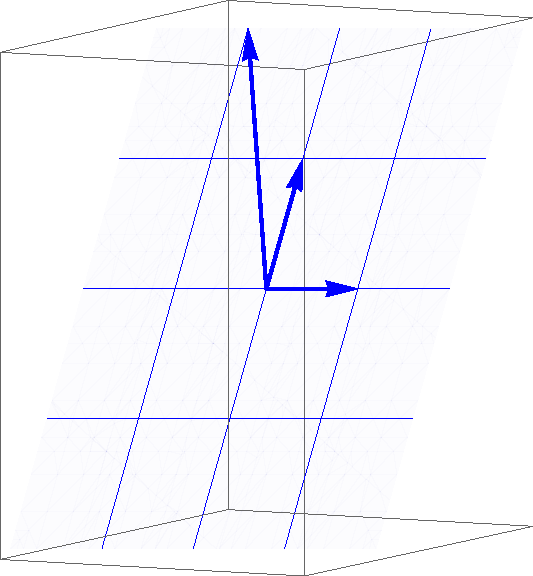
\includegraphics[width=\marginparwidth]{02-Applications/support/colspace1}

Each column of a matrix is a linear combination of the pivot columns.  The coordinates of each column vector are the numbers in the corresponding column of the rref (excluding zero rows).
}
We can write all three columns of the matrix in terms of the basis vectors as 
\begin{align*}
A=\begin{bmatrix}
\cl{1\\2\\0}
&\cl{2\\0\\3}
&\cl{3\\-2\\6}
\end{bmatrix}
&=
\begin{bmatrix}
\begin{bmatrix}\cl{1\\2\\0}&\cl{2\\0\\3}\end{bmatrix}\begin{bmatrix}1\\0\end{bmatrix}&
\begin{bmatrix}\cl{1\\2\\0}&\cl{2\\0\\3}\end{bmatrix}\begin{bmatrix}0\\1\end{bmatrix}&
\begin{bmatrix}\cl{1\\2\\0}&\cl{2\\0\\3}\end{bmatrix}\begin{bmatrix}-1\\2\end{bmatrix}
\end{bmatrix}
\\
&=
\begin{bmatrix}
\cl{1\\2\\0}
&\cl{2\\0\\3}
\end{bmatrix}
\begin{bmatrix}
\cl{1\\0}
&\cl{0\\1}
&\cl{-1\\2}
\end{bmatrix}.
\end{align*}
\end{example}

We see from the example that we can write any matrix as the product of its pivot columns and the nonzero rows of its rref. We can factor any matrix $A$ as $A=CR$, where $C$ is the matrix of pivot columns of $A$ and $R$ is the matrix whose rows are the nonzero rows from $\rref(A)$.

\begin{example}\label{ex:row-space}
Let's find a basis for the row space of the same matrix, 
$$A=\begin{bmatrix}
\cl{1\\2\\0}
&\cl{2\\0\\3}
&\cl{3\\-2\\6}
\end{bmatrix}
\xrightarrow{rref}
\begin{bmatrix}
\cl{1\\0\\0}
&\cl{0\\1\\0}
&\cl{-1\\2\\0}
\end{bmatrix}.
$$
We will see that a basis is the nonzero rows of the rref. Using $A=CR$ as above, and remembering that multiplication can be thought of as linear combinations of rows, we can write  
\begin{align*}
A
=
\begin{bmatrix}
\cl{1\\2\\0}
&\cl{2\\0\\3}
&\cl{3\\-2\\6}
\end{bmatrix}
=
\begin{bmatrix}
\cl{1\\2\\0}
&\cl{2\\0\\3}
\end{bmatrix}
\begin{bmatrix}
\cl{1\\0}
&\cl{0\\1}
&\cl{-1\\2}
\end{bmatrix}
=
\begin{bmatrix}
1\begin{bmatrix}1&0&-1\end{bmatrix} + 2 \begin{bmatrix}0&1&2\end{bmatrix}\\
2\begin{bmatrix}1&0&-1\end{bmatrix} + 0 \begin{bmatrix}0&1&2\end{bmatrix}\\
0\begin{bmatrix}1&0&-1\end{bmatrix} + 3 \begin{bmatrix}0&1&2\end{bmatrix}
\end{bmatrix}
.
\end{align*}

This shows us that every row of the original matrix is a linear combination of the nonzero rows of rref. The row space is the span of the rows, and since the rows of $A$ depend on the nonzero rows of rref, we can span the row space using these nonzero rows. Since the nonzero rows of the rref are linearly independent (placing these rows into columns and reducing won't change the pivots), we know that the nonzero rows of rref form a basis for the row space.  
\marginpar{
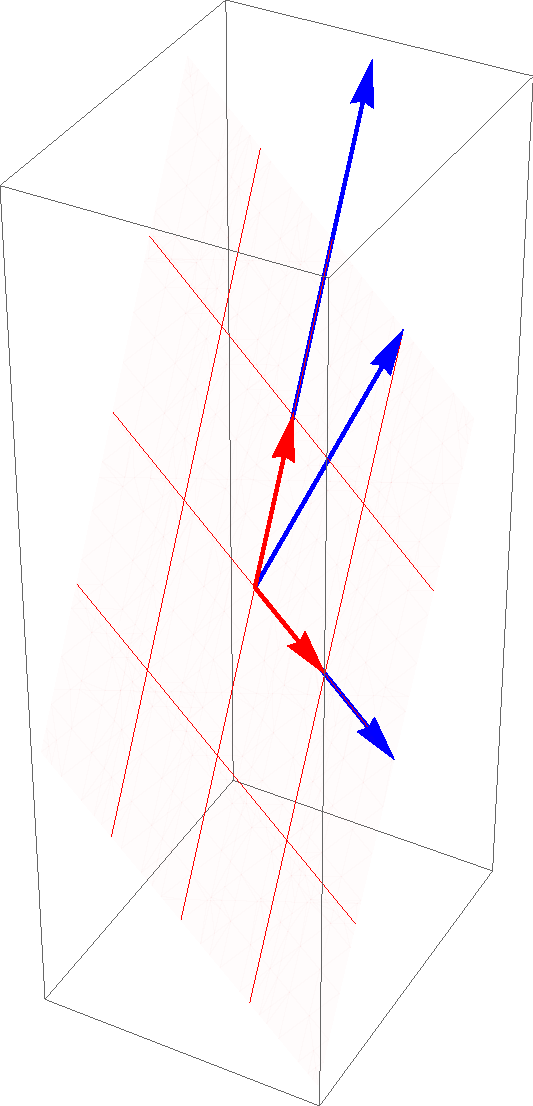
\includegraphics[width=\marginparwidth]{02-Applications/support/rowspace2}

Each row is a linear combination of the nonzero rows of rref.  The coordinates of each row are found in the pivot columns.
}\end{example}

Since the number of pivots (the rank of the matrix) equals the number of nonzero rows in the rref, we can see that the size of the basis for the column space and the size of the basis for the row space are equal.  Therefore the dimensions of the column space and the row space are equal (and are equal to the rank of the matrix).

Let's summarize what we learned in the previous examples.
\begin{enumerate}
	\item The pivot columns are a basis for the column space. 
	\item The nonzero rows of the rref are a basis for the row space.
	\item Every matrix can be decomposed as $A=CR$, where $C$ is a matrix of the pivot columns and $R$ is the nonzero rows of the rref.
	\item The dimension of the column space equals the dimension of the row space, which equals the rank of the matrix.
\end{enumerate}

The transpose of $A$ interchanges the rows and columns, so the row space of $A^T$ is the same as the column space of $A$, and the column space of $A^T$ is the same as the row space of $A$.
 
\begin{example}\label{colspace2ex}
Let's use the transpose to find different bases for the column space and row space of the same matrix from the previous examples:  
$$
A=
\begin{bmatrix}
\cl{1\\2\\0}
&\cl{2\\0\\3}
&\cl{3\\-2\\6}
\end{bmatrix},\quad
A^T
=
\begin{bmatrix}
 1 & 2 & 0 \\
 2 & 0 & 3 \\
 3 & -2 & 6
\end{bmatrix}
\xrightarrow{rref}
\begin{bmatrix}
 1 & 0 & {3}/{2} \\
 0 & 1 & -{3}/{4} \\
 0 & 0 & 0
\end{bmatrix}.
$$
\marginpar{Recall that the coordinates of a vector relative to a basis are the scalars you need to recreate the vector using a linear combination of the basis vectors. Hence the coordinates of $(0,3,6)$ relative to the basis $\{(1,2,3), (2,0,-2)\}$ are $(3/2,-3/4)$ since 
$$\begin{bmatrix}0\\3\\6\end{bmatrix}
=
\frac{3}{2}\begin{bmatrix}1\\2\\3\end{bmatrix}
-
\frac{3}{4}\begin{bmatrix}2\\0\\-2\end{bmatrix}
$$.}%
The set of pivot columns of $A^T$, $\{(1,2,3),\, (2,0,-2)\}$, is a basis for the column space of $A^T$ and the row space of $A$.
The coordinates of the third column of $A^T$ (the third row of $A$), $(0,3,6)$, relative to this basis are $(3/2,-3/4)$. 

The nonzero rows of the rref of $A^T$, namely $\{(1,0,3/2),\, (0,1,-3/4)\}$ are a basis for the row space of $A^T$ and the column space of $A$.  Every column of $A$ can be written as a linear combination of these two vectors. The coordinates of $(1,2,0)$ relative to this basis are $(1,2)$. The coordinates of $(2,0,3)$ are $(2,0)$. The coordinates of $(3,-2,6)$ are $(3,-2)$.
\end{example}

In the last few examples, we have two different ways to obtain a basis for the column space and row space of a matrix. Table~\ref{column and row space table} provides graphs of all 4 bases. You can either reduce $A$ or $A^T$, and use the pivot columns and/or nonzero rows of rref to obtain a basis. Which basis is preferred?  The short answer is ``both.''  Each basis has a different use.  We'll revisit this topic more later.

\begin{table}

\begin{tabular}{ccc}
\multicolumn{3}{c}{
Visualizing two different bases for the column and row space. 
}
\\\hline
\multicolumn{3}{c}{
$
A=
\begin{bmatrix}
\cl{1\\2\\0}
&\cl{2\\0\\3}
&\cl{3\\-2\\6}
\end{bmatrix}
\xrightarrow{rref}
\begin{bmatrix}
\cl{1\\0\\0}
&\cl{0\\1\\0}
&\cl{-1\\2\\0}
\end{bmatrix}
$}
\\ \\
\multicolumn{3}{c}{
$
A^T
=
\begin{bmatrix}
 1 & 2 & 0 \\
 2 & 0 & 3 \\
 3 & -2 & 6
\end{bmatrix}
\xrightarrow{rref}
\begin{bmatrix}
 1 & 0 & {3}/{2} \\
 0 & 1 & -{3}/{4} \\
 0 & 0 & 0
\end{bmatrix}
$
}
\\ \\
\hline\hline \multicolumn{3}{c}{Bases for the column space of $A$, $\col(A)$}\\
\hline Using Pivot Columns of $A$ & Using nonzero rows of rref$(A^T)$ & Both\\ \\
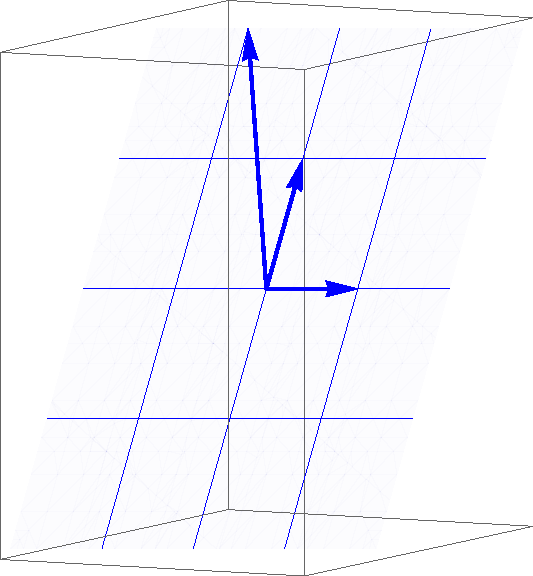
\includegraphics[height=2in]{02-Applications/support/colspace1}
&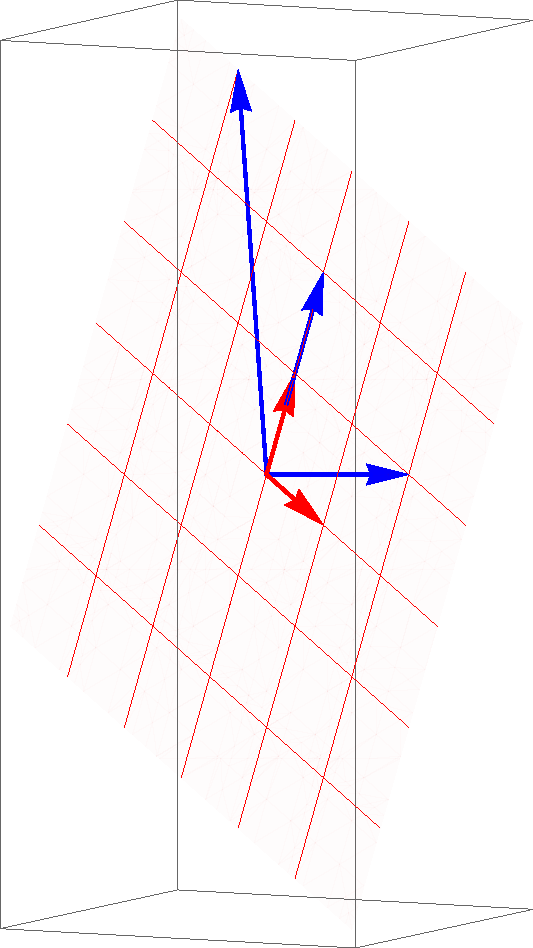
\includegraphics[height=2in]{02-Applications/support/colspace2}
&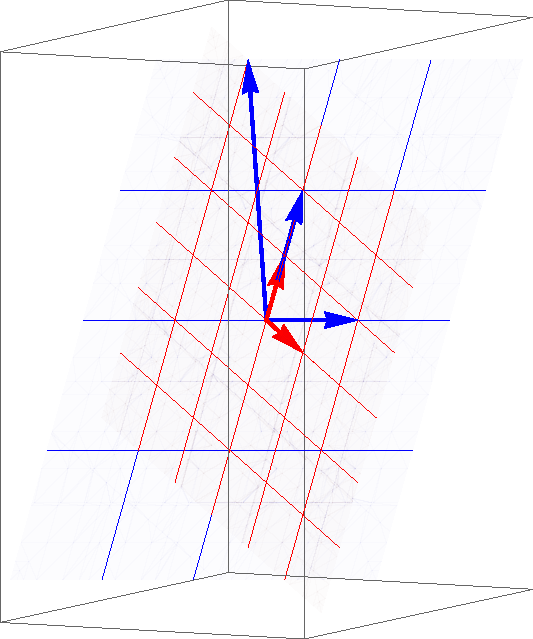
\includegraphics[height=2in]{02-Applications/support/colspace3}
\\ \\
\hline\hline \multicolumn{3}{c}{Bases for the row space of $A$, $\row(A)$}\\
\hline Using Pivot Columns of $A^T$ & Using nonzero rows of rref$(A)$ & Both\\ \\
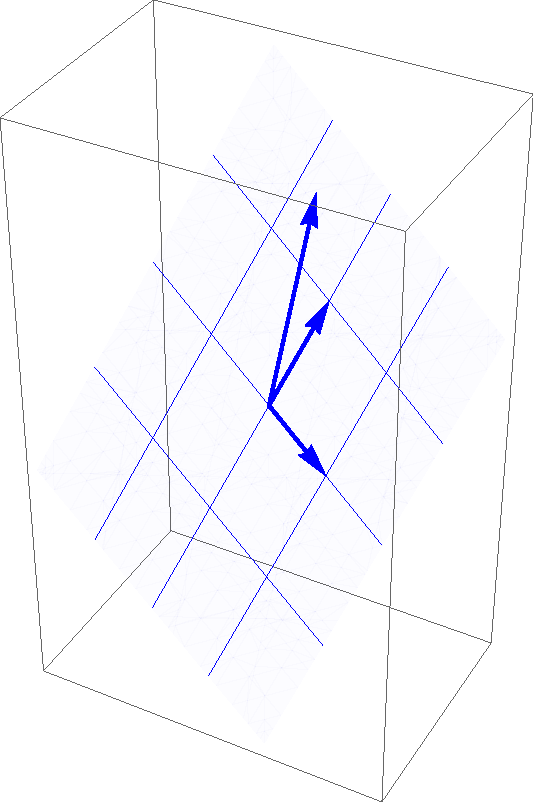
\includegraphics[height=2in]{02-Applications/support/rowspace1}
&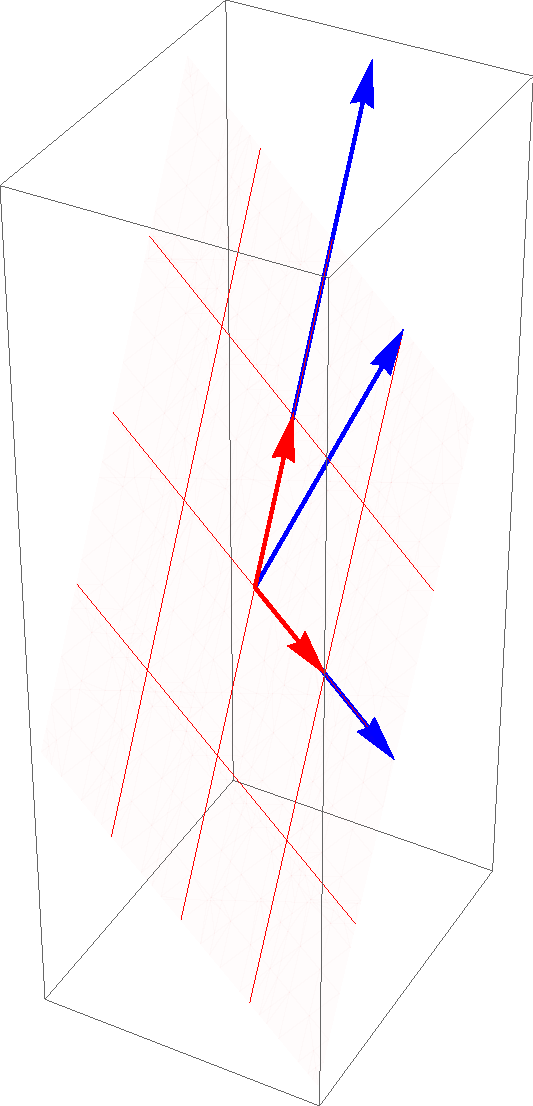
\includegraphics[height=2in]{02-Applications/support/rowspace2}
&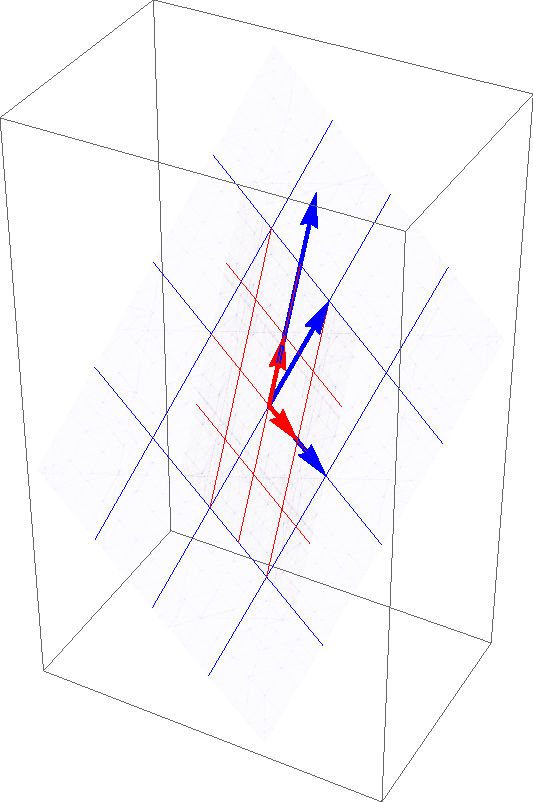
\includegraphics[height=2in]{02-Applications/support/rowspace3}
\end{tabular}

\caption{\label{column and row space table} In examples \ref{colspace1ex}, \ref{ex:row-space}, and \ref{colspace2ex}, we found two different bases for the column and row space. This table shows graphs to help us visualize the differences between these bases.  In all the graphs, the blue vectors represent columns or rows in the matrix and the red vectors represent the vectors in the basis.  
The top row of graphs shows us visualizations of column space where (1) we use the pivot columns to create our basis, (2) we use the nonzero rows of the rref of $A^T$, and (3) both bases are drawn on top of each other.
The bottom row of graphs repeats this visualization for the row space.}
\end{table}

\subsubsection{The null space of a matrix}
The column and row spaces provide two examples of vector
subspaces. These two spaces are defined as the span of a set of
vectors, hence are automatically closed under addition and scalar
multiplication. We'll now explore another set of vectors, called the
null space or kernel of a matrix, where it is not immediately obvious that the set is closed under addition and scalar multiplication.

The \define{null space} (or \define{kernel})
\marginpar{null space=$\nullspace(A)$=$\{\vec x \st A\vec x = \vec 0\}$}%
of a matrix $A$ is the set of vectors $\vec x$ that satisfy the equation $A\vec x=\vec 0$. Notice that the zero vector is always in this set. If there are no other vectors in this set, then we say that null space is the trivial vector space and has dimension zero.  

The null space is closed under addition and scalar multiplication.  If both $\vec x$ and $\vec y$ are in the null space, then $A\vec x=\vec 0$ and $A\vec y=\vec 0$. The sum $\vec x+\vec y$ satisfies 
\begin{align*}
A(\vec x+\vec y)
&= A\vec x+A\vec y &\text{(distribute)}\\
&= \vec 0 +\vec 0 = \vec 0 &(A\vec x = \vec 0 =A\vec y)\\
\end{align*}
This shows that $\vec x+\vec y$ is also in the null space.  
To show that the null space is closed under scalar multiplication, we observe that if $\vec x$ is in the null space and $c$ is any real number, then $$A(c\vec x) = cA\vec x = c\vec 0 = \vec 0,$$
which shows that the null space is closed under scalar multiplication.

We have already seen the null space. Finding eigenvectors requires that we solve $(A-\lambda I)\vec x = 0$, so eigenvectors come from the null space of $A-\lambda I$.  When we compute the null space of $A-\lambda I$, we call it the \define{eigenspace} of $A$ for eigenvalue $\lambda$.

\begin{example}
Let's redo example \ref{eigenvalueexample3} related to eigenvectors, but this time use the vocabulary of null spaces.  
The matrix 
$A=\begin{bmatrix}2&1&4\\ 1&2&4\\ 0&0&1\end{bmatrix}$ has eigenvalues $1,1,3$. 
When $\lambda=1$, we compute $A-\lambda I =\begin{bmatrix}1&1&4\\ 1&1&4\\ 0&0&0\end{bmatrix} $. To find the null space, we solve $(A-\lambda I )\vec x=0$. Row reduction (after augmenting the matrix) gives us the rref $\begin{bmatrix}[ccc|c]1&1&4&0\\ 0&0&0&0\\ 0&0&0&0\end{bmatrix}$, which shows we have two free variables. The solution is $\begin{bmatrix} x_1\\x_2\\ x_3\end{bmatrix} = x_2\begin{bmatrix} -1\\1\\0\end{bmatrix}+x_3\begin{bmatrix} -4\\0\\1\end{bmatrix} $. The null space is this entire solution set (called the eigenspace corresponding to $\lambda = 1$), and is a vector subspace of dimension 2. A basis for the null space is $\{(-1,1,0),\,(-4,0,1)\}$.
Every nonzero vector in this null space is an eigenvector of $A$ with eigenvalue 1.  A similar computation (computing the null space for $A-3I$) shows the eigenspace for $\lambda = 3$ is a one-dimensional vector space with basis $\{(1,1,0)\}$. Example \ref{eigenvalueexample3} has all the details.
\end{example}



\subsection{Why does regression require the transpose?}
We finish this unit with a brief explanation of why we used the transpose to solve the least square regression problem.  We will use the column space of $A$ and the null space of $A^T$. We'll also focus on a specific example in 3D so we can draw pictures.  Later,  we will revisit this idea and develop everything in full generality along with a more powerful vocabulary and theory.  Until then, we'll stick to a visual example.\note{put in a reference to the right chapter}

\marginpar{The two vectors $(1,1,1)$ and $(-2,3,1)$ are orthogonal because their dot product is $-2+3-1=0$.}%
Before getting started, recall that the dot product of two vectors is 0 if and only if the vectors meet at a 90 degree angle. When this occurs, we say that the vectors are orthogonal.
How do you find all the vectors that are orthogonal to a set of vectors $V$? The answer is ``Place all the vectors into the columns of $A$, and then find the null space of $A^T$.'' This null space is called the \define{orthogonal complement} of the set $V$. 
\marginpar{The orthogonal complement to a vector space $V$ is the set of vectors that are orthogonal to every vector in the space.  

The orthogonal complement of the column space of $A$ is the null space of $A^T$.}%

\begin{example}
Let's find all vectors that are orthogonal to $\vec v = (1,2,-3)$.  In other words, we want all vectors $\vec u = (u_1,u_2,u_3)$ such that 
$$
0=(1,2,-3)\cdot(u_1,u_2,u_3) 
=
\begin{bmatrix}1&2&-3\end{bmatrix}
\begin{bmatrix}u_1\\u_2\\u_3\end{bmatrix}
=\vec v^T \vec u
$$
(where $\vec v^T$ is the row matrix with the single row $\vec v$).  This is the same problem as finding the null space of the matrix $v^T=\begin{bmatrix}1&2&-3\end{bmatrix}$. Since the free variables are $u_2$ and $u_3$, we have the solution 
$$
\begin{bmatrix}
u_1\\u_2\\u_3
\end{bmatrix}
=
\begin{bmatrix}
-2u_2+3u_3\\u_2\\u_3
\end{bmatrix}
=u_2
\begin{bmatrix}
-2\\1\\0
\end{bmatrix}
+u_3\begin{bmatrix}
3\\0\\1
\end{bmatrix}
.$$
The set of vectors that are orthogonal to $\vec v$ is a vector space of dimension 2 with basis $\{(-2,1,0),(3,0,1)\}$. This is a plane passing through the origin.
\end{example}

If you are given a set of vectors $\vec v_1,\vec v_2$, how you do find all the vectors that are orthogonal to both?  
If you let $A = [\vec v_1\ \vec v_2]$ (columns of $A$ are the vectors), then a vector $\vec x$ is orthogonal to both $\vec v_1$ and $\vec v_2$ if $A^T\vec x=\vec 0$.
Hence the null space of the transpose of $A$ is the set of vectors that are orthogonal to the columns of $A$.

We're now ready to understand linear regression.


\begin{example}
Recall example \ref{regression1ex}, in which we found the line closest
to passing through the three points $(0,1)$, $(2,4)$, and $(4,5)$.  

In order to find the closest line to several points, the first question is, ``Is there a line that passes through all three points?''  If there is a line $y=a_0+a_1x$ that passes through all of the points, then we have a system of equations
\begin{equation*}
\begin{matrix}a_0=1\\a_0+2a_1=4\\a_0+4a_1=5\end{matrix}
\xrightarrow{\text{augmented matrix}}
\begin{bmatrix}[cc|c]1&0&1\\1&2&4\\1&4&5\end{bmatrix}
\xrightarrow{\text{matrix eqn}}
\begin{bmatrix}1&0\\1&2\\1&4\end{bmatrix}
\begin{bmatrix}a_0\\a_1\end{bmatrix}
=\begin{bmatrix}1\\4\\5\end{bmatrix}.
\end{equation*}
Notice that the system can be written in matrix form $A\vec x = \vec b$, where $A$ contains a column of 1's and $x$-values, $\vec x$ is the vector of coefficients $a_i$, and $\vec b$ is a column of $y$-values.  
\marginpar{Recall that the system $A\vec x=b$ is consistent if $b$ is a linear combination of columns of $A$.}%
The line $y=a_0+a_1x$ passes through the points if there is a solution to $A\vec x=\vec b$ (i.e., the system of equations is consistent).  This will happen if $(1,4,5)$ is in the column space of $A$.  The question ``Is there a line that passes through all of the points?'' is equivalent to asking ``Is $\vec b$ in the column space of $A$?''

However, in this example, $A\vec x=\vec b$ is not consistent since the rref is
\begin{equation*}
\begin{bmatrix}[cc|c]1&0&1\\1&2&4\\1&4&5\end{bmatrix}
\xrightarrow{\rref}
\begin{bmatrix}[cc|c]1&0&0\\0&1&0\\0&0&1\end{bmatrix}.
\end{equation*}
So the answer is ``No, $\vec b$ is not in the column space of $A$.''  Since $\vec b$ is not in the column space of $A$, we ask for the next best thing: ``What vector in the column space of $A$ is closest to $\vec b$?''  In fact, if $\vec b$ is in the column space of $A$, then the answer to the last question is $\vec b$ itself.  So really, the second question is the question we want to answer.  

The key to linear regression is answering the question
\begin{quote}
  What vector $\vec w=A\vec x$ in the column space of $A$ is the closest vector to $\vec b$?
\end{quote}
If $\vec b$ is in the column space of $A$, then the answer is $\vec b$, the system of equation is consistent, we can find $a_0$ and $a_1$, and the line passes through all of the points.  If $\vec b$ is not in the column space of $A$, then we have to do more work.

\marginpar{ \begin{center} \begin{tikzpicture}[x={(0.3cm,0.7cm)},y={(1cm,-0.2cm)},z={(-.5cm,1cm)}]
      \coordinate (origin) at (0,0,0);
      \coordinate (u) at  (1,1,1);
      \coordinate (v) at  (0,2,4);
      \coordinate (b) at  (1,4,5);
      \coordinate (w) at  ($4/3*(u)+(v)$);
      \coordinate (bprime) at ($3*(b)-3*(w)$); % exaggerated b
      \coordinate (r) at ($(b)-(w)$);
    
      \fill[->,fill=lightgray] (origin) -- ($4/3*(u)$) -- (w) -- (v) -- cycle;
      \draw[->] (origin) -- (u);
      \draw[->] (origin) -- (v);
      \draw[->] (origin) -- node[below right, pos=0.9] {$\vec b$} (b) ;
      \draw[->] (origin) -- (u);
      \draw[->] (origin) -- node[left,pos=0.7] {$\vec w$} (w);
      \draw[->] (w) -- node[above right] {$\vec r$} (b);
      

      %right angle
      \draw[thin] ($0.95*(w)$) -- ($0.95*(w)+0.2*(r)$) -- ($(w)+0.2*(r)$);
      % coordinate axes
      %\draw[->,ultra thick] (origin) -- (1,0,0);
      %\draw[->,ultra thick] (origin) -- (0,1,0);
      %\draw[->,ultra thick] (origin) -- (0,0,1);
 \end{tikzpicture}
\end{center}%
%\marginpar{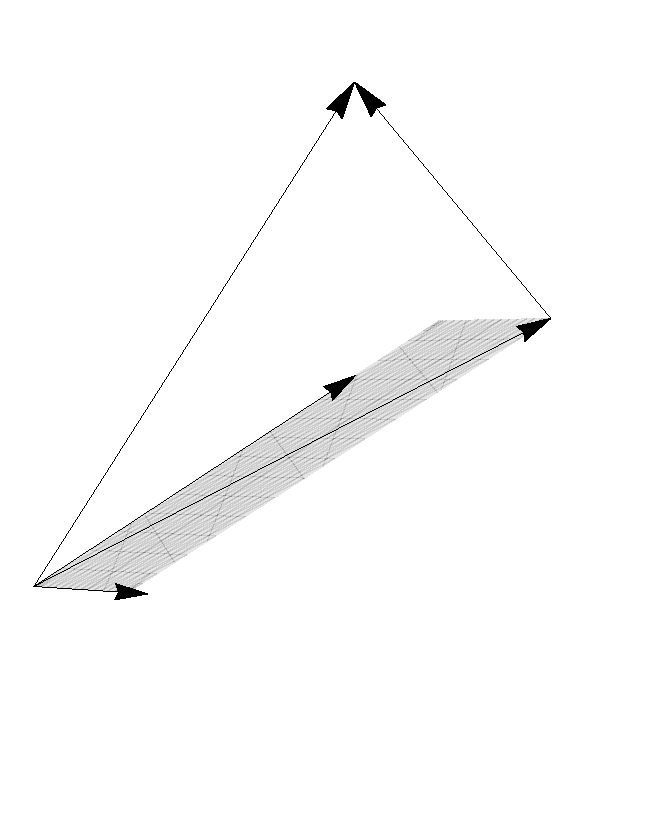
\includegraphics[width=\marginparwidth]{02-Applications/support/regressionpic1}

Because $\vec b$ is not in the column space of $A$, we find the vector $\vec w$ closest to $\vec b$ in the columns space of $A$.  The difference $\vec b-\vec w$ is a vector $\vec r$ that is orthogonal to the column space.}%
To be closest to $\vec b$, a vector $\vec r$ (the ``residual'' vector) with base at $\vec w$ and
head at $\vec b$ must meet the column space of $A$ (a plane) at a 90 degree angle.  So the vector $\vec r = \vec b-\vec w$ is orthogonal to every vector in the column space, or every column of $A$, hence is in the null space of $A^T$ (so $A^T\vec r=\vec 0$). Solving for $\vec w$ gives us $\vec w = \vec b-\vec r$.  Multiplying both sides on the left by $A^T$ and remembering $A\vec x = \vec w$ gives us the regression equation
$$A^TA\vec x=A^T\vec w
=A^T(\vec b-\vec r) 
= A^T\vec b - A^T\vec r 
= A^T\vec b - \vec 0 =
A^T\vec b.$$

Solving for $\vec x$, as before, gives us $\vec x = (a_0,a_1)=(4/3,1)$.
The line closest to the points was $y=\frac{4}{3} + x$. 


The vector $\vec w=A\vec x$ is in the plane spanned by the columns of $A$. Because we already know the solution, in this example we can compute the vector $\vec w$ as
$$
\vec w = A \vec x = \begin{bmatrix}1&0\\1&2\\1&4\end{bmatrix}\begin{bmatrix}4/3\\1\end{bmatrix} = \begin{bmatrix}4/3\\10/3\\16/3  \end{bmatrix}.
$$
We can also compute the residual vector $\vec r=\vec b - \vec w=(-1/3,2/3,-1/3)$, and check that $\vec w \cdot \vec r = (1/9)(-4+20-16)=0$.  The magnitude of the residual vector tells us how close $\vec b$ is to $\vec w$, which gives us an idea of how closely the line fits the points.  In this case, $|\vec r|=\sqrt{2/3}\approx 0.864$.

Note that the vector $\vec x$, $(4/3,1)$, is the vector of coordinates of $\vec w$ relative to the pivot columns of $A$ (here we used the pivot columns of $A$ for our basis).  In the picture in the margin above, the gray parallelogram (part of the plane that is the column space of $A$) was formed by stretching (1,1,1) by $4/3$ and (0,2,4) by $1$, illustrating the linear combination that gives $\vec w$.  

You can think of $\vec w$ as the projection of $\vec b$ onto the column space of $A$.  The solution to the least squares problem, $\vec x$, is the just the vector of coordinates of the projection of $\vec b$ onto the column space of $A$.
Regression is really a problem about projecting a vector onto a vector space, then writing a vector in coordinates relative to a specific basis.


% a pgfplots version of the regression vector picture
 % \begin{tikzpicture}
 %    \begin{axis}[ axis equal =true,xlabel=$x$,ylabel=$y$,view={-10}{30}]
 %      \coordinate (origin) at (axis cs:0,0,0);
 %      \coordinate (u) at  (axis cs:1,1,1);
 %      \coordinate (v) at  (axis cs:0,2,4);
 %      \coordinate (b) at  (axis cs:1,4,5);
 %      \coordinate (w) at  ($4/3*(u)+(v)$);
 %      \coordinate (bprime) at ($3*(b)-3*(w)$);
 %      \addplot3+[arrows=->,mark=none] coordinates {(0,0,0) (1,4,5)};
     
 %      \fill[->,fill=lightgray] (origin) -- ($4/3*(u)$) -- (w) -- (v) -- cycle;
 %      \draw[->] (origin) -- (u);
 %      \draw[->] (origin) -- (v);
 %      \draw[->] (origin) -- node[left, pos=0.9] {$\vec b$} (b) ;
 %      \draw[->] (origin) -- (u);
 %      \draw[->] (origin) -- (w);
 %      \draw[->] (w) -- node[above] {$\vec r$} (b);
      
 %  \end{axis}
 %  \end{tikzpicture}

\end{example}


\section{Summary}
We have used matrix multiplication in all 3 ways:
\begin{enumerate}
\item linear combinations of columns (transition matrices and regression)
\item row dot column (projections in regression)
\item linear combination of rows (electrical networks and curve fitting)
\end{enumerate}
We have seen how Gaussian elimination helps solve problems.  We have seen how the inverse and determinants (Cramer's rule) can rapidly help us find solutions.  We have used eigenvalues and eigenvectors to understand geometric properties like flow in vector fields and maxima and minima of surfaces, as well as find steady state solutions in stochastic processes.  This is a small sample of the beginning of the applications of linear algebra. We also started learning the vocabulary of vector spaces, finding bases and dimensions, which will be the key to extending what we have learned to many more places.  The next unit will help us learn to discover patterns and show us how to use definitions and theorems to explicitly state the patterns we find.  

%%% Local Variables: 
%%% mode: latex
%%% TeX-master: "../linear-algebra"
%%% End: 

\newgeometry{left=1in,right=1in,top=1in,bottom=1in}


\section{Preparation}

\noindent
This chapter covers the following ideas. When you create your lesson plan, it should contain examples which illustrate these key ideas. Before you take the quiz on this unit, meet with another student out of class and teach each other from the examples on your lesson plan. 

\begin{enumerate}

\item Construct visualizations of matrices related to vector fields. Explain how eigenvalues and eigenvectors relate to vector fields.
\item Find the currents in an electrical system involving batteries and resistors, using both Gaussian elimination and Cramer's rule.
\item Find interpolating polynomials. Generalize this curve-fitting process to solve the least squares regression problem of fitting a line to a set of data.
\item Explain how to generalize the derivative to a matrix. Use this
  generalization to locate optimal values of a function using the second derivative test. Explain the role of eigenvalues and eigenvectors in the second derivative test.
\item Describe a Markov process. Explain what a steady-state solution is and how it relates to eigenvectors of the transition matrix.
\item Find bases for the column space, row space, and null space of a matrix and its transpose by row reducing $A$ and $A^T$. Use these bases to find the coordinates of vectors relative to the bases.

\end{enumerate}



%%% Local Variables: 
%%% mode: latex
%%% TeX-master: "../linear-algebra"
%%% End: 


Here are the preparation problems for this unit.  All of these problems come from this book (not Schaum's Outlines).  Remember that solutions appear at the end of each chapter.

%Day 1 we'll only look at matrix multiplication in class.  I'll introduce vector addition, scalar multiplication, the dot product, and then go to linear combinations. This leads immediately to matrix multiplication. Next we will focus on systems of equations and how to solve them.  I'll show how systems can be written in 4 ways, and then reduce a 2 by 2 system.  The next day we will focus on larger systems, and introduce rank and independence.  The next day I'll add in determinants and inverses, and hopefully get to eigenvalues and eigenvectors.   


\begin{center}
\begin{tabular}{ll|l}
\multicolumn{2}{c}{Preparation Problems (\href{http://ilearn.byui.edu/bbcswebdav/institution/Physical\_Sci\_Eng/Mathematics/Personal\%20Folders/WoodruffB/341/2-Applications-Preparation-Solutions.pdf}{click for solutions})}
&
Webcasts 
(
\href{http://ilearn.byui.edu/bbcswebdav/institution/Physical\_Sci\_Eng/Mathematics/Personal\%20Folders/WoodruffB/341/2-Applications-videos.pdf}{pdf copy}
)\\
\hline\hline
Day 1&
1b,
1g,
2c,
3b
&
\href{http://ilearn.byui.edu/bbcswebdav/institution/Physical\_Sci\_Eng/Mathematics/Personal\%20Folders/WoodruffB/341/2-Applications-video-01.wmv}{1},
\href{http://ilearn.byui.edu/bbcswebdav/institution/Physical\_Sci\_Eng/Mathematics/Personal\%20Folders/WoodruffB/341/2-Applications-video-02.wmv}{2},
\href{http://ilearn.byui.edu/bbcswebdav/institution/Physical\_Sci\_Eng/Mathematics/Personal\%20Folders/WoodruffB/341/2-Applications-video-03.wmv}{3}
\\ \hline
Day 2&
4b,
5b,
5d,
6b
&
\href{http://ilearn.byui.edu/bbcswebdav/institution/Physical\_Sci\_Eng/Mathematics/Personal\%20Folders/WoodruffB/341/2-Applications-video-04.wmv}{4},
\href{http://ilearn.byui.edu/bbcswebdav/institution/Physical\_Sci\_Eng/Mathematics/Personal\%20Folders/WoodruffB/341/2-Applications-video-05.wmv}{5},
\href{http://ilearn.byui.edu/bbcswebdav/institution/Physical\_Sci\_Eng/Mathematics/Personal\%20Folders/WoodruffB/341/2-Applications-video-06.wmv}{6}
\\ \hline
Day 3&
6e,
7a,
7b,
8b
&
\href{http://ilearn.byui.edu/bbcswebdav/institution/Physical\_Sci\_Eng/Mathematics/Personal\%20Folders/WoodruffB/341/2-Applications-video-07.wmv}{7},
\href{http://ilearn.byui.edu/bbcswebdav/institution/Physical\_Sci\_Eng/Mathematics/Personal\%20Folders/WoodruffB/341/2-Applications-video-08.wmv}{8},
\href{http://ilearn.byui.edu/bbcswebdav/institution/Physical\_Sci\_Eng/Mathematics/Personal\%20Folders/WoodruffB/341/2-Applications-video-09.wmv}{9}
\\ \hline
Day 4&
8c,
9b,
10b,
11b
&
\href{http://ilearn.byui.edu/bbcswebdav/institution/Physical\_Sci\_Eng/Mathematics/Personal\%20Folders/WoodruffB/341/2-Applications-video-10.wmv}{10},
\href{http://ilearn.byui.edu/bbcswebdav/institution/Physical\_Sci\_Eng/Mathematics/Personal\%20Folders/WoodruffB/341/2-Applications-video-11.wmv}{11}
\\ \hline
Day 6&
Lesson Plan,
Quiz, Start Project &
\\ \hline
\end{tabular}
\end{center}






The problems listed below are found in this book.
\begin{center}
\begin{tabular}{|l|l|l|l|l|}
\hline
Concept&Suggestions&Relevant Problems\\ \hline
Vector Fields&&\ref{vectorfields}\\ \hline
Kirchoff's Laws&&\ref{kirchoff}\\ \hline
Cramer's Rule&&\ref{cramer}\\ \hline
Interpolating Polynomials&&\ref{interpolating}\\ \hline
Least Square Regression&&\ref{regression}\\ \hline
2nd Derivative Test&&\ref{seconddertest}\\ \hline
Stochastic Processes&&\ref{stochastic}\\ \hline
Column and Row Spaces&&\ref{colandrowspace},\ref{coordinates}\\ \hline
Null Space and Projections&&\ref{nullspace},\ref{projections}\\ \hline
\end{tabular}
\end{center}












\section{Problems}
%The problems listed below are found in this book.
%\begin{center}
%\begin{tabular}{|l|l|l|l|l|}
%\hline
%Concept&Suggestions&Relevant Problems\\ \hline
%Kirchoff's Laws&&\ref{kirchoff}\\ \hline
%Cramer's Rule&&\ref{cramer}\\ \hline
%Interpolating Polynomials&&\ref{interpolating}\\ \hline
%Least Square Regression&&\ref{regression}\\ \hline
%Stochastic Processes&&\ref{stochastic}\\ \hline
%2nd Derivative Test&&\ref{seconddertest}\\ \hline
%\end{tabular}
%\end{center}


\begin{enumerate}

\item  {\bf Vector Fields:} \label{vectorfields}For each of the following vector fields, (1) construct a rough plot of the field by graphing the vectors at the 8 points surrounding the origin, (2) find the eigenvalues and eigenvectors, and if real (3) add to your plot the eigenvectors and some flow lines (curves representing the path of motion). Check your work using Sage.
\begin{enumerate}
\begin{multicols}{2}
	\item $F(x,y) = (2x+y,x+2y)$
	\item $F(x,y) = (2x+4y,4x+2y)$
	\item $F(x,y) = (-y,x)$
	\item $F(x,y) = (2x+3y,x+4y)$
	\item $F(x,y) = (2x+3y,4x+1y)$
	\item $F(x,y) = (y,-x)$
	\item $F(x,y) = (x+y,-x+y)$
	\item $F(x,y) = (x-y,x-y)$
	\item $F(x,y) = (x-y,2x-2y)$
	\item $F(x,y) = (-x-y,x-y)$
\end{multicols}
\end{enumerate}


\item  {\bf Kirchoff's Laws:} Consider the following electrical systems. Use the given values to find the current in each wire. \label{kirchoff}

\centerline{\renewcommand{\myscale}{.3}
\begin{tikzpicture}[scale=\myscale,inner sep=1pt]
%\draw[help lines,step=1cm] (0,0) grid (12,6);

%Source - like a battery
\node[label=right:$E$] at (0,3) 
{{\begin{tikzpicture}[scale=\myscale]
%	\useasboundingbox (-.5,-3) rectangle (.5,3);
	\draw (0,0) circle (1cm);
	\draw (.3,.5) -- (-.3,.5);
	\draw (0,.2) -- (0,.8);
	\draw (.3,-.5) -- (-.3,-.5);
	\draw (0,1) -- (0,3);
	\draw (0,-1) -- (0,-3);
	\end{tikzpicture}
}};

%Resistor
\node[label=right:$R_2$] at (6,3) 
{{\begin{tikzpicture}[scale=\myscale]
%	\useasboundingbox (0,-3) rectangle (0,3);
	\draw (0,-3) -- ++(0,1.8) -- ++(.5,.2) 
		-- ++(-1,.4) -- ++(1,.4)
		-- ++(-1,.4) -- ++(1,.4)
		-- ++(-1,.4) -- ++(.5,.2)
		-- ++(0,1.8) ;
	\end{tikzpicture}
}};

%Resistor
\node[label=above:$R_1$] at (3,0) 
{{\begin{tikzpicture}[scale=\myscale,rotate=90]
%	\useasboundingbox (0,-3) rectangle (0,3);
	\draw (0,-3) -- ++(0,1.8) -- ++(.5,.2) 
		-- ++(-1,.4) -- ++(1,.4)
		-- ++(-1,.4) -- ++(1,.4)
		-- ++(-1,.4) -- ++(.5,.2)
		-- ++(0,1.8) ;
	\end{tikzpicture}
}};

%Resistor
\node[label=right:$R_3$] at (12,3) 
{{\begin{tikzpicture}[scale=\myscale,rotate=0]
%	\useasboundingbox (0,-3) rectangle (0,3);
	\draw (0,-3) -- ++(0,1.8) -- ++(.5,.2) 
		-- ++(-1,.4) -- ++(1,.4)
		-- ++(-1,.4) -- ++(1,.4)
		-- ++(-1,.4) -- ++(.5,.2)
		-- ++(0,1.8) ;
	\end{tikzpicture}
}};

%Straight Path
\node at (3,6) 
{{\begin{tikzpicture}[scale=\myscale,rotate=90]
	\draw (0,-3) -- (0,3);
	\end{tikzpicture}
}};

%Straight Path
\node at (9,6) 
{{\begin{tikzpicture}[scale=\myscale,rotate=90]
	\draw (0,-3) -- (0,3);
	\end{tikzpicture}
}};

%Straight Path
\node at (9,0) 
{{\begin{tikzpicture}[scale=\myscale,rotate=90]
	\draw (0,-3) -- (0,3);
	\end{tikzpicture}
}};


%Arrow to represent Current
\node[label=above:$i_1$] at (3,6) 
{{\begin{tikzpicture}[scale=\myscale,rotate=-90]
%	\useasboundingbox (0,-.4) rectangle (0,.4);
	\filldraw (0,.4) -- (-.2,-.4) -- (0,-.3) -- (.2,-.4);
	\end{tikzpicture}
}};

%Arrow to represent Current
\node[label=right:$i_2$] at (6,5) 
{{\begin{tikzpicture}[scale=\myscale,rotate=180]
%	\useasboundingbox (0,-.4) rectangle (0,.4);
	\filldraw (0,.4) -- (-.2,-.4) -- (0,-.3) -- (.2,-.4);
	\end{tikzpicture}
}};

%Arrow to represent Current
\node[label=above:$i_3$] at (9,6) 
{{\begin{tikzpicture}[scale=\myscale,rotate=-90]
%	\useasboundingbox (0,-.4) rectangle (0,.4);
	\filldraw (0,.4) -- (-.2,-.4) -- (0,-.3) -- (.2,-.4);
	\end{tikzpicture}
}};

%Node
\node at (6,6) 
{{\begin{tikzpicture}[scale=\myscale,rotate=-90]
%	\useasboundingbox (0,-.4) rectangle (0,.4);
	\filldraw (0,0) circle (.15cm);
	\end{tikzpicture}
}};

%Node
\node at (6,0) 
{{\begin{tikzpicture}[scale=\myscale,rotate=-90]
%	\useasboundingbox (0,-.4) rectangle (0,.4);
	\filldraw (0,0) circle (.15cm);
	\end{tikzpicture}
}};

\end{tikzpicture}

\renewcommand{\myscale}{.3}
\begin{tikzpicture}[scale=\myscale,inner sep=1pt]
%\draw[help lines,step=1cm] (0,0) grid (18,6);

%Source - like a battery
\node[label=right:$E$] at (0,3) 
{{\begin{tikzpicture}[scale=\myscale]
%	\useasboundingbox (-.5,-3) rectangle (.5,3);
	\draw (0,0) circle (1cm);
	\draw (.3,.5) -- (-.3,.5);
	\draw (0,.2) -- (0,.8);
	\draw (.3,-.5) -- (-.3,-.5);
	\draw (0,1) -- (0,3);
	\draw (0,-1) -- (0,-3);
	\end{tikzpicture}
}};

%Resistor
\node[label=right:$R_2$] at (6,3) 
{{\begin{tikzpicture}[scale=\myscale]
%	\useasboundingbox (0,-3) rectangle (0,3);
	\draw (0,-3) -- ++(0,1.8) -- ++(.5,.2) 
		-- ++(-1,.4) -- ++(1,.4)
		-- ++(-1,.4) -- ++(1,.4)
		-- ++(-1,.4) -- ++(.5,.2)
		-- ++(0,1.8) ;
	\end{tikzpicture}
}};

%Resistor
\node[label=above:$R_1$] at (3,0) 
{{\begin{tikzpicture}[scale=\myscale,rotate=90]
%	\useasboundingbox (0,-3) rectangle (0,3);
	\draw (0,-3) -- ++(0,1.8) -- ++(.5,.2) 
		-- ++(-1,.4) -- ++(1,.4)
		-- ++(-1,.4) -- ++(1,.4)
		-- ++(-1,.4) -- ++(.5,.2)
		-- ++(0,1.8) ;
	\end{tikzpicture}
}};

%Resistor
\node[label=above:$R_3$] at (9,6) 
{{\begin{tikzpicture}[scale=\myscale,rotate=90]
%	\useasboundingbox (0,-3) rectangle (0,3);
	\draw (0,-3) -- ++(0,1.8) -- ++(.5,.2) 
		-- ++(-1,.4) -- ++(1,.4)
		-- ++(-1,.4) -- ++(1,.4)
		-- ++(-1,.4) -- ++(.5,.2)
		-- ++(0,1.8) ;
	\end{tikzpicture}
}};

%Resistor
\node[label=right:$R_4$] at (12,3) 
{{\begin{tikzpicture}[scale=\myscale,rotate=0]
%	\useasboundingbox (0,-3) rectangle (0,3);
	\draw (0,-3) -- ++(0,1.8) -- ++(.5,.2) 
		-- ++(-1,.4) -- ++(1,.4)
		-- ++(-1,.4) -- ++(1,.4)
		-- ++(-1,.4) -- ++(.5,.2)
		-- ++(0,1.8) ;
	\end{tikzpicture}
}};

%Resistor
\node[label=right:$R_5$] at (18,3) 
{{\begin{tikzpicture}[scale=\myscale,rotate=0]
%	\useasboundingbox (0,-3) rectangle (0,3);
	\draw (0,-3) -- ++(0,1.8) -- ++(.5,.2) 
		-- ++(-1,.4) -- ++(1,.4)
		-- ++(-1,.4) -- ++(1,.4)
		-- ++(-1,.4) -- ++(.5,.2)
		-- ++(0,1.8) ;
	\end{tikzpicture}
}};

%Resistor
\node[label=above:$R_6$] at (9,0) 
{{\begin{tikzpicture}[scale=\myscale,rotate=90]
%	\useasboundingbox (0,-3) rectangle (0,3);
	\draw (0,-3) -- ++(0,1.8) -- ++(.5,.2) 
		-- ++(-1,.4) -- ++(1,.4)
		-- ++(-1,.4) -- ++(1,.4)
		-- ++(-1,.4) -- ++(.5,.2)
		-- ++(0,1.8) ;
	\end{tikzpicture}
}};









%Straight Path
\node at (3,6) 
{{\begin{tikzpicture}[scale=\myscale,rotate=90]
	\draw (0,-3) -- (0,3);
	\end{tikzpicture}
}};

%Straight Path
\node at (15,6) 
{{\begin{tikzpicture}[scale=\myscale,rotate=90]
	\draw (0,-3) -- (0,3);
	\end{tikzpicture}
}};

%Straight Path
\node at (15,0) 
{{\begin{tikzpicture}[scale=\myscale,rotate=90]
	\draw (0,-3) -- (0,3);
	\end{tikzpicture}
}};






%Arrow to represent Current
\node[label=above:$i_1$] at (3,6) 
{{\begin{tikzpicture}[scale=\myscale,rotate=-90]
%	\useasboundingbox (0,-.4) rectangle (0,.4);
	\filldraw (0,.4) -- (-.2,-.4) -- (0,-.3) -- (.2,-.4);
	\end{tikzpicture}
}};

%Arrow to represent Current
\node[label=right:$i_2$] at (6,5) 
{{\begin{tikzpicture}[scale=\myscale,rotate=180]
%	\useasboundingbox (0,-.4) rectangle (0,.4);
	\filldraw (0,.4) -- (-.2,-.4) -- (0,-.3) -- (.2,-.4);
	\end{tikzpicture}
}};

%Arrow to represent Current
\node[label=above:$i_3$] at (7,6) 
{{\begin{tikzpicture}[scale=\myscale,rotate=-90]
%	\useasboundingbox (0,-.4) rectangle (0,.4);
	\filldraw (0,.4) -- (-.2,-.4) -- (0,-.3) -- (.2,-.4);
	\end{tikzpicture}
}};

%Arrow to represent Current
\node[label=right:$i_4$] at (12,5) 
{{\begin{tikzpicture}[scale=\myscale,rotate=180]
%	\useasboundingbox (0,-.4) rectangle (0,.4);
	\filldraw (0,.4) -- (-.2,-.4) -- (0,-.3) -- (.2,-.4);
	\end{tikzpicture}
}};

%Arrow to represent Current
\node[label=above:$i_5$] at (15,6) 
{{\begin{tikzpicture}[scale=\myscale,rotate=-90]
%	\useasboundingbox (0,-.4) rectangle (0,.4);
	\filldraw (0,.4) -- (-.2,-.4) -- (0,-.3) -- (.2,-.4);
	\end{tikzpicture}
}};

%Arrow to represent Current
\node[label=above:$i_6$] at (11,0) 
{{\begin{tikzpicture}[scale=\myscale,rotate=90]
%	\useasboundingbox (0,-.4) rectangle (0,.4);
	\filldraw (0,.4) -- (-.2,-.4) -- (0,-.3) -- (.2,-.4);
	\end{tikzpicture}
}};








%Node
\node at (6,6) 
{{\begin{tikzpicture}[scale=\myscale,rotate=-90]
%	\useasboundingbox (0,-.4) rectangle (0,.4);
	\filldraw (0,0) circle (.15cm);
	\end{tikzpicture}
}};

%Node
\node at (6,0) 
{{\begin{tikzpicture}[scale=\myscale,rotate=-90]
%	\useasboundingbox (0,-.4) rectangle (0,.4);
	\filldraw (0,0) circle (.15cm);
	\end{tikzpicture}
}};

%Node
\node at (12,0) 
{{\begin{tikzpicture}[scale=\myscale,rotate=-90]
%	\useasboundingbox (0,-.4) rectangle (0,.4);
	\filldraw (0,0) circle (.15cm);
	\end{tikzpicture}
}};

%Node
\node at (12,6) 
{{\begin{tikzpicture}[scale=\myscale,rotate=-90]
%	\useasboundingbox (0,-.4) rectangle (0,.4);
	\filldraw (0,0) circle (.15cm);
	\end{tikzpicture}
}};

\end{tikzpicture}
}
\begin{multicols}{2}
\begin{enumerate}

\item $E=12, R_1=2,R_2=2, R_3=2$.
\item $E=12, R_1=2,R_2=3, R_3=3$.
\item $E=12, R_1=2,R_2=3, R_3=6$.
\item $E=12, R_1=1,R_2=2, R_3=2$.
\item $E=9, R_1=3,R_2=1, R_3=2$.
\item $E=6, R_1=1,R_2=1, R_3=2$.
\end{enumerate}
\end{multicols}


\begin{enumerate} \setcounter{enumii}{6}
\item $E=12$, $R_1=1$, $R_2=1$, $R_3=1$, $R_4=1$, $R_5=1$, $R_6=1$
\item $E=12$, $R_1=2$, $R_2=1$, $R_3=3$, $R_4=4$, $R_5=2$, $R_6=3$
\end{enumerate}


\item  {\bf Cramer's Rule:}\label{cramer}Use Cramer's rule to find solutions to the following linear systems. If Cramer's rule fails, explain why.

\begin{enumerate}
\begin{multicols}{2}
\item $2x+3y=0, x-2y=1$
\item $x+y=2, x-y=3$
\item $3x+y=6, x+3y=2$
\item $2x+y=1, 4x+2y=2$
\item $x+y=0, 2x-y+z=1, x+z=0$
\item $x+2y=3, x-y+z=0, x+3y+z=1$
\item $y+2z=1, x-z=3, 2x+y=1$
\end{multicols}
\item Re solve any of the problems from problems \ref{kirchoff} or \ref{interpolating} using Cramer's rule.
\end{enumerate}





\item {\bf Interpolating Polynomials:} \label{interpolating}In each of the following scenarios, find a polynomial of least degree which passes through the given points. Verify your result graphically by plotting the points and the polynomial.
\begin{enumerate}
\begin{multicols}{3}
\item $(1,2),(3,3)$ 			
\item $(0,1),(2,3),(-1,4)$  
\item $(1,1),(2,2),(-1,5)$   
\item $(1,2),(3,3),(5,6)$ 			
\item $(1,2),(3,3),(5,5)$ 
\item $(0,1),(1,3),(-1,4),(2,4)$ 
\end{multicols}
\item Select any number of points (with varying $x$ values), and find the interpolating polynomial which goes through them. Check your answer by plugging the points into your polynomial.
\item Open up a spread sheet program (like Microsoft Excel). Make a column of $x$ values and a column of $y$ values. Create a scatter plot of the data and then on your scatter plot add the interpolating polynomial as well as its equation. You can use this to check your answer on any problem you create yourself.
\end{enumerate}



\item {\bf Regression:} \label{regression}For each set of data points, find an equation of the least squares regression line. Plot the points and the line on the same axes. Does the line appear to be the best fit?

\begin{enumerate}
\begin{multicols}{3}
\item $(0,0),(1,3),(1,2)$
\item $(1,1),(2,1),(3,2)$
\item $(1,2),(3,0),(5,1)$
\item $(0,0),(1,3),(1,2),(4,5)$
\item $(0,0),(1,3),(1,2),(4,-5)$
\item $(-1,2),(1,3),(2,5),(3,3)$
\end{multicols}
\item Challenge: Find an equation of the least squares regression parabola $y=a_0+a_1x+a_2x^2$ which passes through the points $(0,0),(1,3),(1,2),(4,5)$. [Hint, you will need a 4 by 3 matrix for $A$ instead of an $n$ by $2$. Use the transpose.]
\end{enumerate}




%\item Compute each integral by finding a partial fraction decomposition. 
%\begin{enumerate}
%\begin{multicols}{2}
%\item $\ds\int\frac{1}{(x-3)(x+2)}dx $%, \frac{A}{x-3}+\frac{B}{x+2}$         
%\item $\ds\int\frac{2x+3}{(x-3)(x+2)}dx$%, \frac{A}{x-3}+\frac{B}{x+2}$ 
%\item $\ds\int\frac{x}{(x+1)(x-2)}dx$%,  \frac{A}{x+1}+\frac{B}{x-2}$  
%\item $\ds\int\frac{x^2+2}{x^2(x-2)}dx$%, \frac{A}{x}+\frac{B}{x^2}+\frac{C}{x-2}$ 
%\item $\ds\int\frac{1}{(x^2+1)(x-2)}dx$%, \frac{Ax+B}{x^2+1}+\frac{C}{x-2}$
%\item $\ds\int\frac{x+1}{(x^2+1)x^2}dx$%, \frac{Ax+B}{x^2+1}+\frac{C}{x}+\frac{D}{x^2}$  
%\end{multicols}
%\end{enumerate}









\item {\bf Second Derivative Test:} \label{seconddertest}For each function, find the location of all critical points. Then use the second derivative test to determine if each critical point corresponds to a maximum, minimum, or saddle point. Graph the function in 3D to verify your results, and locate the eigenvectors and eigenvalues in the picture.
\begin{enumerate}
\begin{multicols}{2}
\item $f(x,y) = x^2+xy+y^2$
\item $f(x,y) = x^2+4xy+y^2$
\item $f(x,y) = x^2+2xy+y^2$
\item $f(x,y) = x^2-4x+y^2+2y+1$
\item $f(x,y) = x^2-2x+xy+y^2$
\item $f(x,y) = x^2+xy+3y^2$
\item $f(x,y) = x^3-3x+y^2-2y$ (2 critical points)
\item $f(x,y) = x^3-3x+y^3-3y^2$ (4 critical points)
\end{multicols}
\item $f(x,y,z)=x^2+xy+y^2+z^2-4z$ (the Hessian will be a 3 by 3 matrix)
\item Create your own function of the form $f(x,y)=Ax^2+Bxy+Cy^2+Dx+Ey+F$.  Find the critical points and determine if they correspond to a maximum, minimum, or saddle point. 
\item For what values of $A,B,C,D,E,F$ will $f(x,y)=Ax^2+Bxy+Cy^2+Dx+Ey+F$ have a critical point that corresponds to a minimum? a maximum? a saddle point? When will the second derivative test fail? How does $B^2-4AC$ relate to this problem? [Hint: the quadratic formula will prove useful in trying to find the eigenvalues symbolically.  How does the product of the eigenvalues relate to the determinant of the Hessian?]
\end{enumerate}







\item  {\bf Markov Processes:}\label{stochastic} In each scenario, write the transition matrix. If an initial state is given, then find the next two states. Finish by finding a steady state solution and use it to answer the question at the end.
%\begin{multicols}{2}
\begin{enumerate}

\item In a certain town, there are 3 types of land zones: residential, commercial, and industrial. The city has been undergoing growth recently, and the city has noticed the following trends.  Every 5 years, 10\% of the older residential land gets rezoned as commercial land, while 5\% gets rezoned as industrial.  The other 85\% remains residential.  For commercial land, 70\% remains commercial, while 10\% becomes residential and 20\% becomes industrial. For industrial land, 60\% remains industrial, while 25\% becomes commercial and 15\% becomes residential. Currently the percent of land in each zone is 40\% residential, 30\% commercial, and 30\% industrial. What will the percent distribution be in 5 years? In 10 years?  If this trend continues indefinitely, what percent of the land will eventually be residential?. 
\item Suppose we own a car rental company which rents cars in Idaho Falls and Rexburg. The last few weeks have shown a weekly trend that 60\% of the cars rented in Rexburg will remain in Rexburg (the other 40\% end up in IF), whereas 80\% of the cars rented in Idaho Falls will remain in Idaho Falls. If there are currently 60 cars in Rexburg and 140 cars in IF, how many will be in each city next week?  In two weeks? In three weeks? If this trend continues indefinitely, about how many cars should you expect to find in Rexburg each week?
\item Repeat the previous problem if 40\% of the cars rented in Rexburg will remain in Rexburg (the other 60\% end up in IF), whereas 80\% of the cars rented in Idaho Falls will remain in Idaho Falls.
\item Repeat the previous problem if 70\% of the cars rented in Rexburg will remain in Rexburg (the other 30\% end up in IF), whereas 80\% of the cars rented in Idaho Falls will remain in Idaho Falls.
\item A school cafeteria regularly offers 3 types of meals to its students. One of the meals is always a pizza/salad combo, One is always hamburgers and fries, and one is a daily special which changes daily. In an attempt to understand student preferences, the school discovered the following information. If a student has a hamburger one day, then there is a 30\% chance they will try the daily special the next day, and a 40\% percent chance they will have the salad bar.  If they have the salad bar, then there is a 30\% chance they'll switch to the daily special, and a 40\% chance they'll switch to the hamburger.  If the have the daily special, then there is a 50\% chance they'll get the daily special the next day, a 20\% chance they'll switch to pizza, and a 30\% chance they'll switch to hamburger.  If this trend continues, what percent of the students will eat each type of meal? 

[While this problem is highly rigged, there is a branch of applied mathematics which is studied by financial analysts call stochastic processes which models such a scenario. This modeling process can help predict how a new restaurant will perform in a city, sometimes predict stock market fluctuations, and more. The study of stochastic processes begins with a Markov chain and then introduces statistics and probability to help predict what happens when trends change.]
\end{enumerate}
%\end{multicols}




\item  {\bf Column and Row Spaces:} \label{colandrowspace}For each matrix, find the reduced row echelon form of both $A$ and $A^T$.  Use your results to give two bases for the column space. Then give two bases for the row space. If you feel like you have mastered row reduction, then please use a computer (practice using Sage) to do the row reduction for you so that you can focus on just being able to pick out the two different bases. 

\begin{enumerate}
\begin{multicols}{3}
\item 
$\begin{bmatrix}
 2 & 3 & 1 \\
 -3 & -5 & 3
\end{bmatrix}
$

\item
$
\begin{bmatrix}
 2 & 4 & 1 \\
 1 & 2 & 3
\end{bmatrix}
$

\item
$
\begin{bmatrix}
 1 & 2 & 3 \\
 2 & 0 & 1 \\
 -3 & -2 & -4
\end{bmatrix}
$

\item
$
\begin{bmatrix}
 1 & 3 & 2 \\
 2 & 1 & 0 \\
 -3 & -4 & -2
\end{bmatrix}
$

\item
$
\begin{bmatrix}
 2 & 1 & -2 & 4 \\
 1 & 3 & 0 & 5 \\
 -2 & 1 & 1 & 2
\end{bmatrix}
$

\item
$
\begin{bmatrix}
 0 & 1 & 2 & 3 \\
 2 & -1 & -4 & 0 \\
 -1 & 2 & 5 & 5
\end{bmatrix}
$

\end{multicols}
\end{enumerate}


\item  {\bf Coordinates of a vector relative to a basis:} \label{coordinates} For this problem, use the same matrices as problem 8.  From the columns of $A$, select a basis for the column space of $A$. Then give the coordinates of $\vec v$ and $\vec w$ relative to this basis, or explain why the vector is not in the column space of $A$.  
\begin{enumerate}
\begin{multicols}{3}
\item 
$\vec v = (2, 1)$ ,\\
$\vec w = (-1, 3)$


\item 
$\vec v = (6, 3)$ ,\\
$\vec w = (-1, 3)$

\item 
$\vec v = (3, -4, 1)$ ,\\
$\vec w = (-1, 3, 2)$

\item 
$\vec v = (3, -4, 1)$ ,\\
$\vec w = (3, -3, 0)$

\item 
$\vec v = (0, 8, 10)$ ,\\
$\vec w = (-13, -9, 2)$

\item 
$\vec v = (-7, 0, -12)$ ,\\
$\vec w = (-8, 11, -18)$
\end{multicols}
\end{enumerate}



\item  {\bf Null Space, Eigenspace, and Orthogonal Complement:} \label{nullspace}By finding the solutions to either $A\vec x=\vec 0$ (the null space), $(A-\lambda I)\vec x = \vec 0$ (an eigenspace), or $A^T\vec x = \vec 0$ (an orthogonal complement), find a basis and the dimension of the vector subspace requested.

$$
A= \begin{bmatrix}
 0 & -4 & -4 \\
 9 & 2 & -1 \\
 -3 & 0 & 1
\end{bmatrix}
,
B=\begin{bmatrix}
 2 & 4 & -4 & -7 \\
 3 & 6 & 1 & 0 \\
 -1 & -2 & 1 & 2 \\
 0 & 0 & 8 & 12
\end{bmatrix}
,
C=
\begin{bmatrix}
 2 & 0 & 4 & 2 \\
 -1 & -6 & 1 & -4 \\
 2 & -2 & 5 & 1
\end{bmatrix}
, 
D=
\begin{bmatrix}
 0 & 4 & 4 \\
 3 & -2 & -5 \\
 1 & 4 & 3 \\
 -2 & 0 & 2
\end{bmatrix}
$$

\begin{enumerate}
\begin{multicols}{2}
\item Find a basis for the null space of $A$.
\item Find a basis for the null space of $B$.
\item Find a basis for the null space of $C$.
\item Find a basis for the null space of $D$.
\end{multicols}
\item Find a basis for the set of vectors that are orthogonal to the columns of $A$.
\item Find a basis for the set of vectors that are orthogonal to the columns of $B$.
\item Find a basis for the set of vectors that are orthogonal to the columns of $C$.
\item Find a basis for the set of vectors that are orthogonal to the columns of $D$.

\item For
$
\begin{bmatrix}
 2 & -1 & 1 \\
 -1 & 2 & 1 \\
 -2 & -2 & 5
\end{bmatrix}
$, find a basis for the eigenspace corresponding to $\lambda = 3$.

\item For
$
\begin{bmatrix}
 -4 & 8 & 6 \\
 -9 & 14 & 9 \\
 6 & -8 & -4
\end{bmatrix}
$, find a basis for the eigenspace corresponding to $\lambda = 2$.




\end{enumerate}



\item {\bf Projections:} \label{projections}Let $\vec w$ be the projection of $\vec b$ onto the column space of $A$.  Find the coordinates of $\vec w$ relative to the columns of $A$. Then state the vector $\vec w$. Check that you are correct by showing that $\vec n = \vec b-\vec w$ is orthogonal to the columns of $A$ (i.e. show $A^T\vec n=\vec 0$). Compare to problem \ref{regression}
\begin{enumerate}
\item 
\begin{multicols}{3}

$A=
\begin{bmatrix}
\cl{1\\1\\1}&
\cl{0\\1\\1}
\end{bmatrix}
$, 
$\vec b = 
\begin{bmatrix}
\cl{0\\3\\2}
\end{bmatrix}
$

\item 
$A=
\begin{bmatrix}
\cl{1\\1\\1}&
\cl{1\\2\\3}
\end{bmatrix}
$, 
$\vec b = 
\begin{bmatrix}
\cl{1\\1\\2}
\end{bmatrix}
$


\item 
$A=
\begin{bmatrix}
\cl{1\\1\\1}&
\cl{1\\3\\5}
\end{bmatrix}
$, 
$\vec b = 
\begin{bmatrix}
\cl{2\\0\\1}
\end{bmatrix}
$


\item 
$A=
\begin{bmatrix}
\cl{1\\1\\1\\1}&
\cl{0\\1\\1\\4}
\end{bmatrix}
$, 
$\vec b = 
\begin{bmatrix}
\cl{0\\3\\2\\5}
\end{bmatrix}
$


\item 
$A=
\begin{bmatrix}
\cl{1\\1\\1\\1}&
\cl{0\\1\\1\\4}
\end{bmatrix}
$, 
$\vec b = 
\begin{bmatrix}
\cl{0\\3\\2\\-5}
\end{bmatrix}
$


\item 
$A=
\begin{bmatrix}
\cl{1\\1\\1\\1}&
\cl{-1\\1\\2\\3}
\end{bmatrix}
$, 
$\vec b = 
\begin{bmatrix}
\cl{2\\3\\5\\3}
\end{bmatrix}
$

\end{multicols}


\end{enumerate}


\end{enumerate}




\section{Projects}
\begin{enumerate}

%This will be updated shortly.  It will involve using the computer to explore how Sage finds basis vectors for a vector space. We'll explore the difference between using $A$ and $A^T$, and why a computer uses $A^T$ instead of $A$.  We'll give a reason for why one is called the standard or cannonical basis.
%
%Goal of project.  Learn how to determine if two basis for a vector space are the same.  Different computers give different basis.  The answers in the back of the book may be different.  A vector space is a huge collection of vectors, and there are infinitely many ways to give a basis for the vector space.  So how do we determine if two vector spaces are the same?  The idea is to use rref.  Once you have a basis, place the vectors in rows and row reduced the matrix.  When you are finished, you will have obtained a basis for the row space.  Any other vectors in this space must depend on these vectors, so if you place additional vectors in the matrix as additional rows, then again you should not obtain anything different.  If you start with a different basis, row reduce that matrix.  If it's rref is the same as the first, you have the same space.  If the rref's are not the same, you have a different space.
%
%Now I need to write this up so that they give me what I just said.



	\item Consider the matrices
$A=
\begin{bmatrix}
 2 & 4 & -4 & -7 \\
 3 & 6 & 1 & 0 \\
 -1 & -2 & 1 & 2 \\
 0 & 0 & 8 & 12
\end{bmatrix}
$ and 
$B=
\begin{bmatrix}
 -4 & -7 & 2 & 4 \\
 1 & 0& 3 & 6  \\
 1 & 2& -1 & -2  \\
 8 & 12& 0 & 0 
\end{bmatrix}
$. Because both matrices have the same columns (just in a different order), the column space of $A$ and the column space of $B$ both represent the same vector subspace. There are infinitely many vectors in this subspace, so there are infinitely many ways to find a basis. Is there a standard basis, one that we can compare any other basis to in an easy manner?  The problems below will help you discover this basis.

\begin{enumerate}
	\item \label{project2A} Find a basis for the column space of $A$ by selecting the pivot columns.
	\item \label{project2B} Find a basis for the column space of $B$ by selecting the pivot columns.
	\item Find a basis for the column space of $A$ by reducing $A^T$. 
	\end{enumerate}
	
	You should now have 3 different bases. The next 5 problems should all result in the same basis.
	\begin{enumerate}[resume]
	\item Find a basis for the column space of $B$ by reducing $B^T$.
	\item Let $C$ be a matrix whose columns are the basis vectors obtained in part (a). Row reduce the transpose to obtain a different basis. 
	\item Let $D$ be a matrix whose columns are the basis vectors obtained in part(b). Row reduce the transpose to obtain a different basis.
	\item Interchange the columns of $A$ in some other way.  Row reduce the transpose of your matrix to obtain a basis for the column space of $A$.
	\item Joe claims that a basis for the column space is 
	$\{(-5,3,1,12),(0,7,-1,8)\}$.  Is he correct?  To answer this, place his vectors in the columns of a matrix and then row reduce the transpose.  
\end{enumerate}

The basis obtained above is called the standard basis for the column space of $A$. Any time someone gives you a basis for a vector subspace of $\mathbb{R}^n$, you can obtain the standard basis using the ideas above.  Just place the  vectors into the columns of matrix, and then reduce the transpose. Alternatively, just place the vectors into the rows of a matrix, and then reduce the matrix. 




 



\end{enumerate}


{
\section{Solutions}
\small
Here are the solutions

\begin{multicols}{2}
\begin{enumerate}
\item Vector Fields:  
\newcommand{\myvfwidth}{1.5in}
\begin{enumerate}
\item $3, (1,1),  5, (-1,1)$\\ 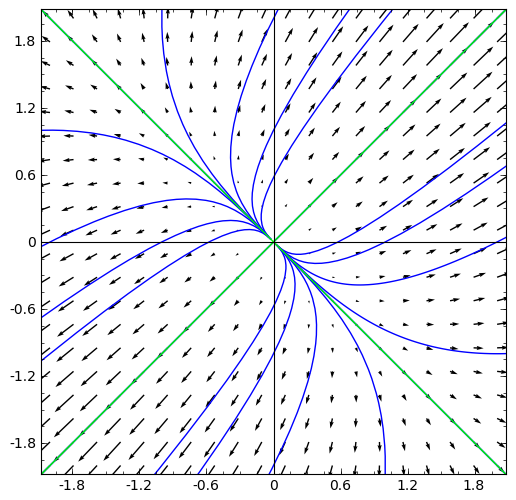
\includegraphics[width=\myvfwidth]{02-Applications/support/vfa}
\item $6, (1,1),  -2, (-1,1)$\\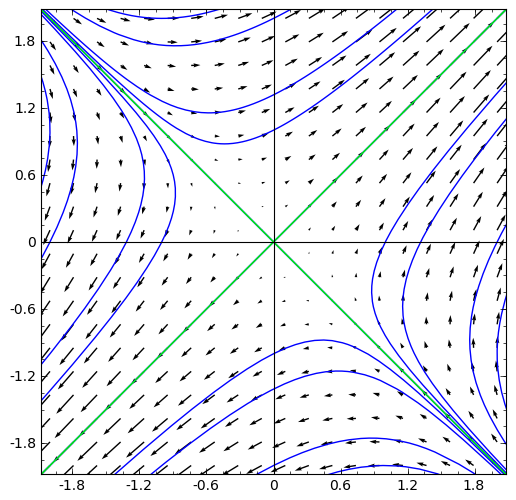
\includegraphics[width=\myvfwidth]{02-Applications/support/vfb}
\item $i, (i,1),  -i, (-i,1)$\\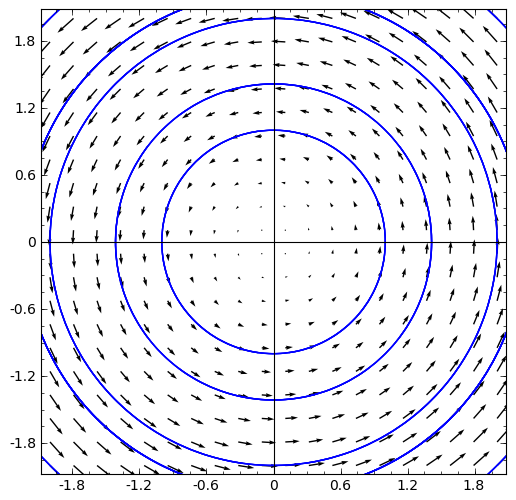
\includegraphics[width=\myvfwidth]{02-Applications/support/vfc}
\item $5, (1,1),  1, (-3,1)$\\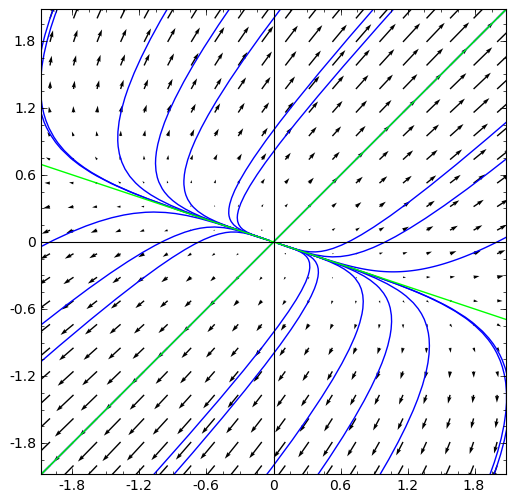
\includegraphics[width=\myvfwidth]{02-Applications/support/vfd}
\item $5, (1,1),  -2, (-3/4,1)$\\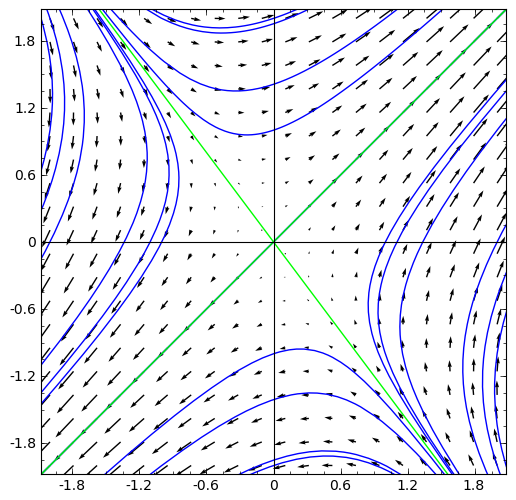
\includegraphics[width=\myvfwidth]{02-Applications/support/vfe}
\item $i, (-i,1),  -i, (i,1)$\\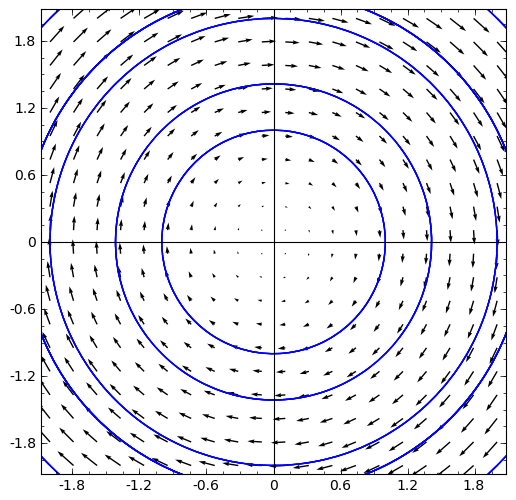
\includegraphics[width=\myvfwidth]{02-Applications/support/vff}
\item $1+i, (-i,1), 1-i, (i,1)$\\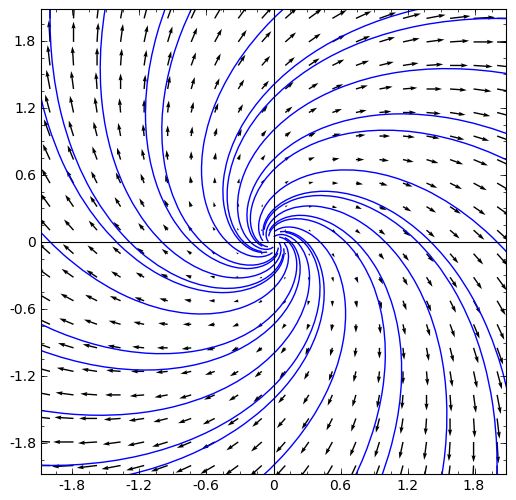
\includegraphics[width=\myvfwidth]{02-Applications/support/vfg}
\item $0, (1,1)$, there only one independent eigenvectors. \\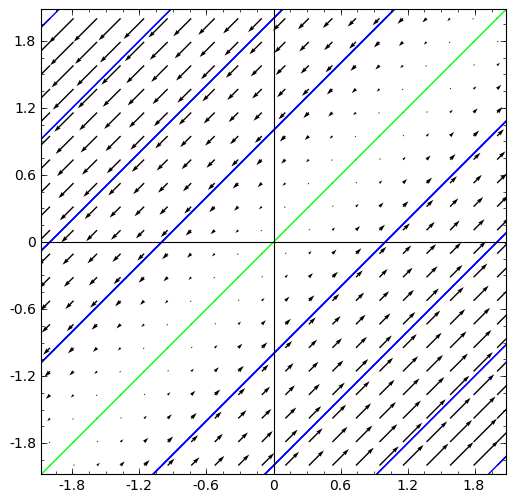
\includegraphics[width=\myvfwidth]{02-Applications/support/vfh}
\item $0, (1,1),  -1, (1,2)$\\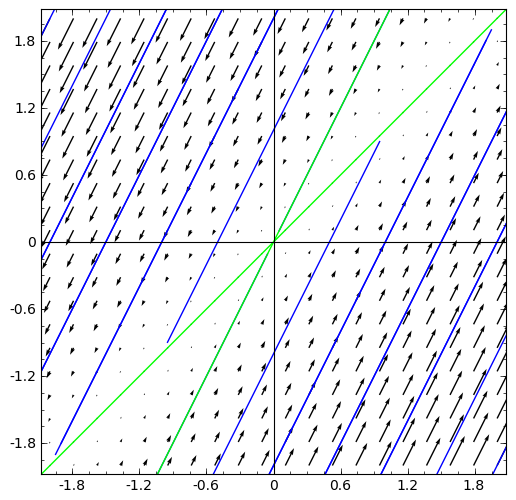
\includegraphics[width=\myvfwidth]{02-Applications/support/vfi}
\item $-1+i, (1,-i),  -1-i, (1,i)$\\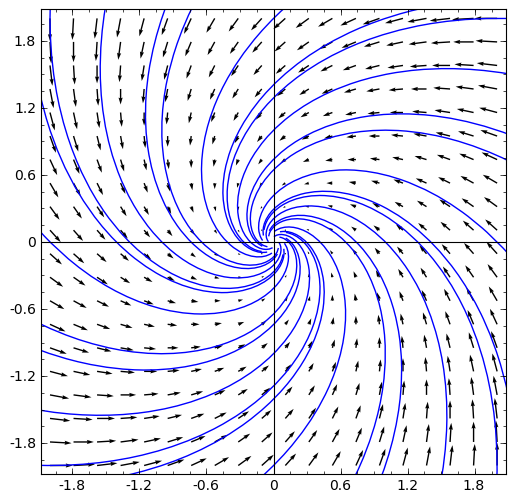
\includegraphics[width=\myvfwidth]{02-Applications/support/vfj}
\end{enumerate}


\item Kirchoff's Laws

 $\begin{bmatrix}[lll|l]
 1 & -1 & -1 & 0 \\
 R_1 & R_2 & 0 & E \\
 0 & -R_2 & R_3 & 0
\end{bmatrix}$

\begin{enumerate}
\item $(4,2,2)$
\item $(24/7,12/7,12/7)$
\item $(3,2,1)$
\item $(6,3,3)$
\item $(27/11,18/11,9/11)$
\item $(18/5,12/5,6/5)$

$\begin{bmatrix}[llllll|l]
 1 & -1 & -1 & 0 & 0 & 0 & 0 \\
 0 & 0 & 1 & -1 & -1 & 0 & 0 \\
 0 & 0 & 0 & 1 & 1 & -1 & 0 \\
 R_1 & R_2 & 0 & 0 & 0 & 0 & E \\
 0 & -R_2 & R_3 & R_4 & 0 & R_6 & 0 \\
 0 & 0 & 0 & -R_4 & R_5 & 0 & 0
\end{bmatrix}$

\item $\left\{7, 5, 2, 1, 1, 2\right\}$

\item $\left\{\frac{25}{6},\frac{11}{3},\frac{1}{2},\frac{1}{6},\frac{1}{3},\frac{1}{2}\right\}$
\end{enumerate}


\item Cramer's rule
\begin{enumerate}
\item $\left\{\frac{3}{7},-\frac{2}{7}\right\}$
\item $\left\{\frac{5}{2},-\frac{1}{2}\right\}$
\item $\{2,0\}$
\item Fails. The determinant of the coefficient matrix is zero.
\item $\left\{\frac{1}{2},-\frac{1}{2},-\frac{1}{2}\right\}$
\item $\left\{\frac{5}{2},\frac{1}{4},-\frac{9}{4}\right\}$
\item Fails. The determinant of the coefficient matrix is zero.
\end{enumerate}





\item Interpolating Polynomials
\begin{enumerate}
\item $1/2 x + 3/2$
\item $(4/3)x^2-(5/3)x+1$
\item $x^2-2x+2$
\item $(1/4)x^2-(1/2)x+9/4$
\item $(1/8)x^2+15/8$
\item $-x^3+(5/2)x^2+(1/2)x+1$
\end{enumerate}


\item Regression (Make the plots using technology)
\begin{enumerate}
\item $y=\frac{5 x}{2}$
\item $y=\frac{x}{2}+\frac{1}{3}$
\item $y=\frac{7}{4}-\frac{x}{4}$
\item $y=\frac{10 x}{9}+\frac{5}{6}$
\item $y=\frac{5}{2}-\frac{5 x}{3}$
\item $y=\frac{3 x}{7}+\frac{19}{7}$
\item 
$
A=
\begin{bmatrix} 
 0 & 0 & 1 \\
 1 & 1 & 1 \\
 1 & 1 & 1 \\
 16 & 4 & 1
\end{bmatrix},
B=
\begin{bmatrix} 
 0 \\
 3 \\
 2 \\
 5
\end{bmatrix},
A^T A=
\begin{bmatrix} 
 258 & 66 & 18 \\
 66 & 18 & 6 \\
 18 & 6 & 4
\end{bmatrix},
A^T B=
\begin{bmatrix} 
 85 \\
 25 \\
 10
\end{bmatrix}$,

$y=-\frac{5}{12}x^2+\frac{35}{12}x+0
$
\end{enumerate}






%\item Partial Fractions
%\begin{enumerate}
%\item $-1/5\,\ln  \left( x+2 \right) +1/5\,\ln  \left( x-3 \right)$
%\item $1/5\,\ln  \left( x+2 \right) +9/5\,\ln  \left( x-3 \right) $
%\item $1/3\,\ln  \left( x+1 \right) +2/3\,\ln  \left( x-2 \right) $
%\item ${x}^{-1}+3/2\,\ln  \left( x-2 \right) -1/2\,\ln  \left( x \right)$
%\item $-\frac{1}{10}\ln  \left( {x}^{2}+1 \right) -\frac{2}{5}\arctan \left( x \right) +\frac{1}{5}\ln  \left( x-2 \right) $
%\item $-{x}^{-1}-1/2\,\ln  \left( {x}^{2}+1 \right) -\arctan \left( x
% \right) +\ln  \left( x \right)
%$
%\end{enumerate}



\item Second Derivative Test
\begin{enumerate}
\item At $(0,0)$ eigenvalues are $3,1$ (both positive so min) with eigenvectors $[1,1]^T,[-1,1]^T$.
\item At $(0,0)$ eigenvalues are $6,-2$ (saddle point) with eigenvectors $[1,1]^T,[-1,1]^T$.
\item At $(0,0)$ eigenvalues are $4,0$ (test fails) with eigenvectors $[1,1]^T,[-1,1]^T$.
\item At $(2,-1)$ eigenvalues are $2,2$ (both positive so min) with eigenvectors $[1,0]^T,[0,1]^T$.
\item At $(4/3,-2/3)$ eigenvalues are $3,1$ (both positive so min) with eigenvectors $[1,1]^T,[-1,1]^T$.
\item At $(0,0)$ eigenvalues are $6.23607,1.76393$ (both positive so min) with eigenvectors $[.236,1]^T,[-4.236,1]^T$.
\item 
At $(-1,1)$ eigenvalues are $-6,2$ (saddle) with eigenvectors $[1,0]^T,[0,1]^T$.
At $(1,1)$ eigenvalues are $6,2$ (both positive so min) with eigenvectors $[1,0]^T,[0,1]^T$.
\item 
At $(-1,0)$ eigenvalues are $-6,-6$ (both negative so max) with eigenvectors $[1,0]^T,[0,1]^T$.
At $(-1,2)$ eigenvalues are $-6,6$ (saddle) with eigenvectors $[1,0]^T,[0,1]^T$.
At $(1,0)$ eigenvalues are $6,-6$ (saddle) with eigenvectors $[1,0]^T,[0,1]^T$.
At $(1,2)$ eigenvalues are $6,6$ (both positive so min) with eigenvectors $[1,0]^T,[0,1]^T$.

\end{enumerate}






\item Markov Processes

\begin{enumerate}
\item Transition matrix 
$\begin{bmatrix}
 0.85 & 0.1 & 0.15 \\
 0.1 & 0.7 & 0.25 \\
 0.05 & 0.2 & 0.6
\end{bmatrix}$,
5 years  (41.5,32.5,26), 
10 years: (42.425,33.4,24.175),
Steady state: $[4,3,2]^T$ so 4/9 or 44.4\% will be residential. 

\item
Transition matrix 
$\begin{bmatrix}
 {3}/{5} & {1}/{5} \\
 {2}/{5} & {4}/{5}
\end{bmatrix}$,
1 week  (64,136), 
2 week: (65.6,134.4),
3 week: (66.24,133.76),
Steady state: $[1,2]^T$ so 1/3 (33.3\%) will be in Rexburg. This means 66 or 67 cars will be in Rexburg. 
 
\item 
Transition matrix 
$\begin{bmatrix}
 {2}/{5} & {1}/{5} \\
 {3}/{5} & {4}/{5}
\end{bmatrix}$,
1 week  (52,148), 
2 week: (50.4,149.6),
3 week: (50.08,149.92),
Steady state: $[1,3]^T$ so 1/4 or 25\% will be in Rexburg. This means 50 cars will be in Rexburg. 

\item 
Transition matrix 
$\begin{bmatrix}
 {7}/{10} & {1}/{5} \\
 {3}/{10} & {4}/{5}
\end{bmatrix}$,
1 week  (70,130), 
2 week: (75,125),
3 week: (77.5,122.5),
Steady state: $[2,3]^T$ so 2/5 or 40\% will be in Rexburg. This means 80 cars will be in Rexburg. 

\item My order is hamburger, pizza/salad, special (your order may vary which means your matrix will be a little different, but the eigenvector will still have the same ratios).
Transition matrix 
$\begin{bmatrix}
 {3}/{10} & {2}/{5} & {3}/{10} \\
 {2}/{5} & {3}/{10} & {1}/{5} \\
 {3}/{10} & {3}/{10} & {1}/{2}
\end{bmatrix}$,
Steady state: $[29,26,33]^T$ or $[29/88,26/88,33/88]^T$ so Hamburger - 32.9545\%, Pizza/Salad - 29.5455\%, Special - 37.5\%. 

\end{enumerate}







\item  {\bf Column and Row Spaces:} 

\begin{enumerate}
\item Col: 
$\{  (2, -3), (3, -5)  \}$,
$\{  (1, 0), (0, 1),  \}$.
\\Row:
$\{  (1, 0, 14), (0, 1, -9)  \}$,
$\{  (2, 3, 1), (-3, -5, 3)  \}$.

\item Col: 
$ \{  (2, 1),  (1, 3)  \} $,
$ \{  (1, 0), (0, 1)  \} $.
\\Row:
$ \{  (1, 2, 0), (0, 0, 1)  \} $,
$ \{  (2, 4, 1), (1, 2, 3)  \} $.

\item Col: 
$ \{  (1, 2, -3), (2, 0, -2)  \} $,
$ \{  (1, 0, -1), (0, 1, -1)  \} $.
\\Row:
$ \{  (1, 0, 1/2), (0, 1, 5/4) \} $,
$ \{  (1, 2, 3), (2, 0, 1)  \} $.

\item Col: 
$ \{  (1, 2, -3), (3, 1, -4)  \} $,
$ \{  (1, 0, -1), (0, 1, -1)  \} $.
\\Row:
$ \{  (1, 0, -(2/5)), (0, 1, 4/5)  \} $,
$ \{  (1, 3, 2), (2, 1, 0) \} $.

\item Col: 
$ \{  (2, 1, -2), (1, 3, 1), (-2, 0, 1) \} $,
$ \{  (1, 0, 0), (0, 1, 0), (0, 0, 1)  \} $.
\\Row:
$ \{  (1, 0, 0, -1), (0, 1, 0, 2), (0, 0, 1, -2)  \} $,
$ \{  (2, 1, -2, 4), (1, 3, 0, 5), (-2, 1, 1, 2)  \} $.

\item Col: 
$ \{  (0, 2, -1), (1, -1, 2), (3, 0, 5)  \} $,
$ \{  (1, 0, 0), (0, 1, 0), (0, 0, 1)  \} $.
\\Row:
$ \{  (1, 0, -1, 0), (0, 1, 2, 0), (0, 0, 0, 1)  \} $,
$ \{  (0, 1, 2, 3), (2, -1, -4, 0) \} $.

\end{enumerate}


\item  {\bf Coordinates of a vector relative to a basis:} The basis vectors are the pivot columns of rref. See 8 for the basis vectors. To get the coordinates, augment $A$ by the two vectors, and row reduce. 
\begin{enumerate}
\item  
$\vec v: (13, -8)$,
$\vec w: (4, -3) $

\item  
$\vec v: (3, 0)  $,
$\vec w: (-(6/5), 7/5)$

\item  
$\vec v: (-2, 5/2) $,
$\vec w: $ not in space.

\item  
$\vec v: (-3, 2)$,
$\vec w: (-(12/5), 9/5)$

\item  
$\vec v: (-4, 4, -2)$,
$\vec w: (0, -3, 5)$

\item  
$\vec v: (1, 2, -3) $,
$\vec w: (3, -5, -1) $

\end{enumerate}



\item  {\bf Null Space, Eigenspace, and Orthogonal Complement:} There is more than one way to pick a basis. Here possible answers. I obtained these basis by writing solutions in terms of the free variable (rrefing $A$ or $A^T$) and then multiplying by the least common denominator to eliminate fractions.
\begin{enumerate}
\item $\{ (1, -3, 3)\}$
\item $\{ (1, 0, -3, 2), (-2, 1, 0, 0)\}$
\item $\{ (-2, -1, 0, 2), (-4, 1, 2, 0)\}$
\item $\{ (1, -1, 1)\}$

\item $\{ (1, 2, 6)\}$
\item $\{ (12, -8, 0, 7), (2, 1, 7, 0)\}$
\item $\{ (-7, -2, 6)\}$
\item $\{ (1, 2, 0, 3), (-7, -2, 6, 0)\}$

\item $\{ (1, 0, 1), (-1, 1, 0)\}$
\item $\{ (1, 0, 1), (4, 3, 0)\}$

\end{enumerate}



\item {\bf Projections:} The work is identical to problem \ref{regression}. The only difference is the vocabulary. I'll give the coordinates of $\vec w$ as well as $\vec w$
\begin{enumerate}
\item 
Coor: $(0,5/2)$,\\
$\vec w = 5/2(0,1,1)$

\item 
Coor: $(1/3, 1/2)$,\\
$\vec w = 1/3(1,1,1)+1/2(1,2,3)$

\item 
Coor: $(7/4, -1/4)$,\\
$\vec w = 7/4(1,1,1)-1/4(1,3,5)$

\item 
Coor: $(5/6,10/9)$,\\
$\vec w = 5/6(1,1,1,1)+10/9(0,1,1,4)$

\item 
Coor: $(5/2,-5/3)$,\\
$\vec w = 5/2(1,1,1,1)-5/3(0,1,1,4)$

\item 
Coor: $(19/7, 3/7)$,\\
$\vec w =19/7(1,1,1,1)+3/7(-1,1,2,3)$

\end{enumerate}










	
\end{enumerate}


\end{multicols}
}





\restoregeometry
\chapter{Patterns}


The purpose of this chapter is to help you learn to create examples of patterns that others before you have noticed. Vector spaces are the most important pattern we will explore in this chapter.


\begin{enumerate}

\item Create examples to illustrate mathematical definitions. Know these definitions.
\item Create examples to illustrate theorems. You do not have to memorize all the theorems, rather when one is given make sure you can construct examples of it. 
\item When a matrix has an inverse, this is equivalent to many other facts about the matrix and corresponding systems of equations.  Illustrate this equivalence with examples, and be able to explain why the the ideas are equivalent.
\item Be able to explain why something is or is not a vector space. Give examples of vector spaces and subspaces that you have encountered previously in this class and other classes.
\item Explain how to find a basis for a vector space and the dimension of a vector space. Give the coordinates of vectors relative to a chosen basis.

\end{enumerate}


\section{Recognizing and Naming Patterns}

Have you ever noticed while reading a mathematics or other science textbook that the book is filled with the following four things: (1) examples, (2) definitions, (3) theorems, and (4) proofs? One of the main goals of mathematics is to describe the patterns in the world around us, and these four things are often the ways a pattern is found and communicated.  

Most of the time, recognizing a pattern starts with an example.  After working with lots of examples, you start to notice recurring patterns. Once you pinpoint exactly what the pattern is, you create a definition to explicitly describe the pattern. When you can describe exactly when and how a patterns appear, or if you can describe how different patterns relate to each other, you create a theorem. Proofs provide the logical backbone to the theorems. Everything in this process starts with examples.  

Learning mathematics requires learning to work with examples. The main goal of this chapter is to learn how to create examples to understand the definitions and theorems that others have discovered.  If you encounter a new idea in any scientific area, start by looking at examples.  After you have studied several simple examples, you will discover patterns that help you understand the new idea.  Sometimes, your exploration of simple examples will result in new discoveries (theorems). Examining, understanding, and generalizing from examples is one of the main tools of mathematical and scientific research.  Learning to create and look at examples is crucial.

The most important pattern in linear algebra is the notion of a vector space. This is an abstract space that came from studying the properties of vectors in $\mathbb{R}^n$, and then realizing that these same properties hold in other places (like polynomials, functions, waves, and more). Before we formally define a vector space in general, we will practice creating examples to understand definition and theorems.  Most of what follows is a summary of the ideas introduced in the previous chapters. As you encounter each new definition or theorem, your homework will be to create an example which illustrates the new idea.  Once we have done this, we'll be ready to formally define vector spaces. Then the real power of linear algebra begins.


%
%Mathematical discoveries begin with examples. However, mathematical writing often begins with definitions. Those definitions are followed by theorems and proofs. If space permits, examples are often given to illustrate the definitions and theorems.  If appropriate, an application (example) is also given to show why a theorem is important. Those who write mathematical papers and textbooks around the nation have become accustomed to writing papers for peers in journals. Most of the time, these papers assume a lot of knowledge from the reader, and because of space limitations the papers are missing lots of examples. In order to read this kind of mathematics, you have to learn how to create examples to illustrate definitions and theorems whenever you see them.

%In this section, most of the definitions and theorems you have already seen and used in the previous chapters. The next three subsections present definitions, theorems, and then proofs. In the definitions and theorems section, I will provide examples of some of the ideas (or point you to examples from previous chapters). Your homework is to create examples to illustrate the definitions and theorems. In the proofs section, I will illustrate a few common techniques that are used to prove theorems.  The proofs in linear algebra are often shorter and easier to follow than proofs in other branches of mathematics. Those of you who plan to pursue any type of graduate study in engineering, physics, computer science, economics, statistics, and more will be expected to give proofs of the ideas you discover. In this book I will provide only some of the proofs and let you seek other references to find complete proofs to all the ideas. 



\subsection{Definitions}

Whenever you see a new definition, one of the most important things you can do is create an example which illustrates that definition. As you read each definition below, create an example which illustrates that definition. Most of these words are review, but a few are new.  Make sure you know these definitions.

This first definition is a formal statement of what we mean when we write $\mathbb{R}^n$.  It is the foundation for the formal vector space definition we'll see later.
\begin{definition}[Real Vector Space]
The symbol $\mathbb{R}$ is used to represent the real numbers.  
The \define{real vector space} $\mathbb{R}^n$ is a set together with a way of adding two elements (called \define{vector addition}) and a way of multiplying an element by a real number (called \define{scalar multiplication}).  
The set we use is the set of $n$-tuples $(v_1,v_2,\ldots, v_n)$ where each $v_i$ is an element of $\mathbb{R}$. 
We write this symbolically as 
$$
\{ (v_1,v_2,\ldots, v_n)\st v_i\in \mathbb{R} \text{ for } 1\leq i\leq n\}.$$
Each $n$-tuple $\vec v = (v_1,v_2,\ldots, v_n)$ is called a vector. 
The entries of the vector are called the \define[vector!components]{components} of the vector.  Vector addition is performed by adding the components of the vectors. Scalar multiplication is done by multiplying each component by the scalar. 
\end{definition}


\begin{definition} 
\marginpar{See example \ref{ex dot product}.}%
\label{def dot product}
The \define{dot product} of two vectors $\vec u = \left<u_1,u_2,\ldots,u_n\right>$ and $\vec v =\left<v_1,v_2,\ldots,v_n\right>$ is the scalar $\vec u\cdot \vec v = u_1v_1+u_2v_2+\cdots+u_nv_n = \sum u_iv_i$. We say that two vectors are \define{orthogonal} if their dot product is zero.
\end{definition}

\begin{definition} \label{def matrix product} 
A (real) \define{matrix} is a rectangular grid of real numbers.
We use the notation $a_{ij}$ to represent the entry in the $i$th row and $j$th column of the matrix $A$.  
If a matrix $A$ has $m$ rows and $n$ columns, we say the matrix has \define[matrix!size]{size} $m$ by $n$ and write $A_{mn}$. 
The \define[matrix!sum]{sum} of two matrices of the same size is performed by adding corresponding entries.  
The \define[matrix!product]{product} of two matrices $A_{m n} = \left\{a_{ij}\right\}$ and $B_{np} =\left\{b_{jk}\right\}$\note{braces?  I thought square brackets were more normal.} is a new matrix $C=AB$ where the $ik$th entry of $C$ is $c_{ik}=\sum_{j=1}^n a_{ij}b_{jk}$ (the dot product of the $i$th row of $A$ and the $k$th column of $B$).
\end{definition}

\begin{definition} \label{def rref}
\marginpar{See example \ref{ex rref last}. Every matrix we obtain in the row reduction process of $A$ is row equivalent to all the other matrices obtained from $A$ by doing row operations, and to the reduced row echelon form of $A$. Each of the matrices in example \ref{ex rref last} is row equivalent to all the other matrices in the example.}%
We say that two matrices are \define[matrix!row equivalent]{row equivalent} if one can be obtained from the other by a finite sequence of these three row operations: (1) interchange two rows, (2) multiply one row by a nonzero constant, and (3) add to a row a multiple of a different row. 

A matrix is said to be in \define{row echelon form} (ref) if 
(1) each nonzero row begins with a 1 (called a \define{leading 1}), 
(2) the leading 1 in a row occurs further right than a leading 1 in the row above, and
(3) any rows of all zeros appear at the bottom.
The location in the matrix of each leading 1 is called a \define{pivot}, and the column containing the pivot is called a \define{pivot column}.
A matrix is said to be in \define{reduced row echelon form} (rref) if 
the matrix is in row echelon form, and each pivot column contains all zeros except for the pivot (the leading one).

\end{definition}

\begin{definition}[Homogeneous]
A linear system $A\vec x=\vec b$ is said to be either \define{homogeneous} if $\vec b=\vec 0$ or \define{nonhomogeneous} if $\vec b\neq \vec 0$.  
\end{definition}
\begin{definition}[Consistent]
A linear system is said to be \define{consistent} if it has at least one solution and  \define{inconsistent} if it has no solutions.
\end{definition}



\begin{definition}[Linear combination, Span]
\marginpar{See example \ref{ex span}.}%
A \define[vectors!linear combination]{linear combination} of vectors $\{\vec v_1,\vec v_2,\ldots,\vec v_n\}$ is a sum $$c_1 \vec v_1+c_2\vec v_2+\cdots+c_n\vec v_n = \sum_{i=1}^n c_i\vec v_i$$ where each scalar $c_1,c_2,\ldots, c_n$ is a real number. 
The \define{span} of a set of vectors $\{\vec v_1,\vec v_2,\ldots,\vec v_n\}$ is the set of all possible linear combinations of those vectors.
\end{definition}

\begin{definition}[Linear independence] 
\marginpar{See example \ref{first linearly independent example}. }%
We say a set $\{\vec v_1,\vec v_2,\ldots,\vec v_n\}$ of vectors is \define{linearly independent} if the only solution to the homogeneous equation $c_1 \vec v_1+c_2\vec v_2+\cdots+c_n\vec v_n=\vec 0$ is the trivial solution $c_1=c_2=\cdots=c_n=0$. If there is a nonzero solution to this homogeneous equation, then we say the set of vectors is \define{linearly dependent}, or we just say the vectors are linearly dependent (leave off ``set of'').
\end{definition}

\begin{definition}[Basis]
A \define{basis} for $\mathbb{R}^n$ is a set of vectors that are (1) linearly independent and (2) span all of $\mathbb{R}^n$.
The \define{standard basis} for $\mathbb{R}^n$ is the set 
$$\{\vec e_1 = (1,0,0,\ldots,0,0) , 
\vec e_2 = (0,1,0,\ldots,0,0) , 
\ldots, 
\vec e_n = (0,0,0,\ldots,0,1)\}.$$
\end{definition}

\begin{definition}[Column space, Rank] 
\marginpar{See examples \ref{colspace1ex} and \ref{colspace2ex}.}%
The \define{column space} of a matrix is the span of the column vectors. 
A \definestyle{basis for the column space} of a matrix is a set of linearly independent vectors whose span is the column space. 
The \definestyle{dimension} of the column space is the number of vectors in a basis for the column space. 
The \define{rank} of a matrix is the dimension of the column space.
\end{definition}


\begin{definition}[Row space] 
\marginpar{See examples \ref{colspace1ex} and \ref{colspace2ex}.}%
The \define{row space} of a matrix is the span of the row vectors. 
A \definestyle{basis for the row space} is a set of linearly independent vectors whose span is the row space. 
The \definestyle{dimension} of the row space is the number of vectors in a basis for the row space.
\end{definition}

\begin{definition}[Coordinates]
\marginpar{See examples \ref{colspace1ex} and \ref{colspace2ex}.}%
If $\beta=\{\vec b_1,\vec b_2,\ldots,\vec b_n\}$ is a basis for a vector space, and a vector $\vec v$ equals the linear combination 
$$ \vec v = c_1\vec b_1+c_2\vec v_2 + \cdots c_n\vec v_n, $$ then we call the scalars $c_1,c_2,\ldots, c_n$ the  \define{coordinates} of $\vec v$ relative to the basis $\beta$. We may write $\vec v = (c_1,c_2,\ldots, c_n)_\beta$ to represent the vector $\vec v$, or if the basis $\beta$ is understood, we may just write $\vec v = (c_1,c_2,\ldots, c_n)$.
\end{definition}

\begin{definition}[Diagonal, Identity, Triangular matrices]
A \define[matrix types!diagonal]{diagonal matrix} is a square matrix where the entries off the main diagonal are zero ($a_{ij}=0$ if $i\neq j$). The \define[matrix types!identity]{identity matrix} is a diagonal matrix where each entry on the main diagonal is 1 ($a_{ii}=1$). We often write $I$ to represent the identity matrix, and $I_n$ to represent the $n\times n$ identity matrix when specifying the size is important. An \define[matrix types!upper triangular]{upper triangular matrix} is a square matrix where every entry below the main diagonal is zero. A \define[matrix types!lower triangular]{lower triangular matrix} is a square matrix where every entry above the main diagonal is zero.
$$\begin{array}{cccc}
\begin{bmatrix} 3&0&0\\0&-2&0\\0&0&8\end{bmatrix} 
&\begin{bmatrix} 1&0&0\\0&1&0\\0&0&1\end{bmatrix} 
&\begin{bmatrix} 0&3&2\\0&4&0\\0&0&-1\end{bmatrix}
&\begin{bmatrix} 0&0&0\\3&4&0\\2&0&-1\end{bmatrix} 
\\
\text{diagonal}
&\text{identity}
&\text{upper-triangular}
&\text{lower-triangular}
\end{array}$$
\end{definition}



\begin{definition}[Determinant] 
\marginpar{See example \ref{ex det}.}%
The \define{determinant} of a $1\times 1$ matrix is the entry $a_{11}$. A \define{minor} $M_{ij}$ of an $n\times n$ matrix is the determinant of the $(n-1)\times (n-1)$ submatrix obtained by removing the $i$th row and $j$th column. A \define{cofactor} of a matrix is the product $C_{ij}=(-1)^{i+j}M_{ij}$. The determinant of an $n\times n$ matrix ($n\geq 2$) is found by multiplying each entry $a_{1i}$ on the first row of the matrix by its corresponding cofactor, and then summing the result. Symbolically we write  $$\det A = |A| = a_{11}C_{11}+a_{12}C_{12}+\cdots+a_{1n}C_{1n} = \sum_{j=1}^n a_{1j}C_{1j}.$$ 
\end{definition}


\begin{definition}[Inverse] 
\marginpar{See example \ref{ex inverse}}%
The \define{inverse} of a square matrix $A$ is a matrix $B$ such that $AB=I$ and $BA=I$, where $I$ is the identity matrix. If a square matrix does not have an inverse, we say the matrix is \define{singular} or \define{noninvertible}. 
\end{definition}

\begin{definition}[Transpose]
\marginpar{See example \ref{ex transpose}.}%
The \define[matrix!transpose]{transpose} of a matrix $A_{m\times n}=\{a_{ij}\}$ is a new matrix $A^T_{n\times m}$ where the $i$th column of $A$ is the $i$th row of $A^T$.  A \define[matrix types!symmetric]{symmetric matrix} is a matrix $A$ such that $A=A^T$.
\end{definition}


\begin{definition}[Eigenvector, Eigenvalue] 
\marginpar{See examples \ref{ex eigen1} and \ref{ex eigen2.}
  Note that $\vec x=\vec 0$ is never an eigenvector.}%
An \define{eigenvector} of a square matrix $A$ is a nonzero vector $\vec x$ with the property that $A\vec x = \lambda \vec x$ for some scalar $\lambda$.  We say that $\vec x$ is an \define{eigenvector} corresponding to the \define{eigenvalue} $\lambda$. 
\end{definition}





















%%%%%%%%%%%%%%%%Theorems
%%%%%%%%%%%%%%%%Theorems
%%%%%%%%%%%%%%%%Theorems
%%%%%%%%%%%%%%%%Theorems
%%%%%%%%%%%%%%%%Theorems
%%%%%%%%%%%%%%%%Theorems
%%%%%%%%%%%%%%%%Theorems
%%%%%%%%%%%%%%%%Theorems
%%%%%%%%%%%%%%%%Theorems
%%%%%%%%%%%%%%%%Theorems
%%%%%%%%%%%%%%%%Theorems
%%%%%%%%%%%%%%%%Theorems


\subsection{Theorems}

The definitions above summarize most of what we have done in the first two chapters. The list of properties below summarize many of the patterns we have already observed, together with many patterns that we will be exploring as the semester progresses.  Each is called a theorem because it is a statement that requires justification (a proof). In the homework, your job is to create examples to illustrate these theorems.  If a theorem is hard to remember, then create more examples to illustrate the theorem until you recognize the patterns that emerge.  Mathematics is all about finding patterns and then precisely stating the pattern in words. You do not have to memorize all of these theorems, but you should be able to create examples to illustrate them. In the next section, we will prove some of them.

Before stating the theorems, we first need to discuss the phrase ``if and only if.'' Theorem \ref{every column pivot iff independent} states 
\begin{quote}
The columns are linearly independent if and only if every column is a pivot column.
\end{quote}
We could write this statement symbolically by writing ``$p$ if and only if $q$.''
\marginpar{The statement ``$p$ if and only if $q$'' implies both 
\begin{enumerate}
	\item if $p$ then $q$, and 
	\item if $q$ then $p$.
\end{enumerate}
}
The words if and only if create two if then statements, namely (1) if $p$ then $q$ and (2) if $q$ then $p$. This gives us the two statments:
\begin{enumerate}
	\item If the columns are linearly independent then every column is a pivot column.
	\item If every column is a pivot column then the columns are linearly independent.
\end{enumerate}
Every time you see the words ``if and only if,'' remember that this means you have two if-then statements.  That means that you need at least two examples to illustrate such a theorem (one for each if-then statement).



\subsubsection{Vector Properties}
\begin{theorem}[Vector space properties of $\mathbb{R}^n$]\label{rn vector space properties}
Vector addition and scalar multiplication in $\mathbb{R}^n$ satisfy the following properties:
\begin{enumerate}
	\item[($A_1$)] Vector addition is associative: $(\vec u+\vec v)+\vec w = \vec u +(\vec v+\vec w)$.
	\item[($A_2$)] Vector addition is commutative: $\vec u+\vec v= \vec v+\vec u$.
	\item[($A_3$)] The zero vector $\vec 0$ satisfies $\vec 0+\vec v = \vec v+\vec 0=\vec v$.
	\item[($A_4$)] The additive inverse of $\vec v$, denoted $-\vec v$, is the vector which satisfies $\vec v+(-\vec v)=0$.
	\item[($M_1$)] Scalar multiplication distributes across vector addition: $c(\vec u+\vec v)= c\vec u + c\vec v$.
	\item[($M_2$)] Scalar multiplication distributes across scalar addition: $(c+d)\vec v= c\vec v+ d\vec v$.
	\item[($M_3$)] Scalar multiplication is associative: $(cd)\vec v = c(d\vec v)$
	\item[($M_4$)] Scalar multiplication by 1 does nothing: $1\vec v=\vec v$
\end{enumerate}
\end{theorem}

\subsubsection{System Properties}
 
\begin{theorem}\label{thm unique rref}
Every matrix has a unique reduced row echelon form (rref). This implies that for any matrix, the location of the pivot columns is unique (they do not depend on how the matrix is reduced to rref). 
\end{theorem}

\begin{theorem}\label{thm row equivalent}
Two matrices are row equivalent if and only if they have the same reduced row echelon form.
\end{theorem}


\begin{theorem} \label{pivot columns iff} \label{thm solution iff augmented not pivot}
A linear system of equations $A\vec x=\vec b$ has a solution if and only if the number of pivot columns of $A$ equals the number of pivot columns of the augmented matrix $[A|b]$.
\end{theorem}

\begin{theorem}\label{thm no, one, or infinitely many solutions}
If a linear system of equations has more than one solution, it has infinitely many.  Solving a linear system has three possible outcomes: (1) no solution, (2) exactly one solution, or (3) infinitely many solutions. 
\end{theorem}

\begin{theorem}[Removing non pivot columns does not alter the row operations involved in obtaining rref.] Let $A$ be a matrix whose rref is $R$.  Let $B$ be the matrix obtained from $A$ by removing the $k$th column.  If the $k$th column of $A$ is not a pivot column, then the rref of $B$ is found by removing the $k$th column from $R$. 
\end{theorem}

\begin{theorem}\label{thm n-k free variables}
If a consistent linear system of equations $A\vec x=\vec b$ has $n$ variables and $k$ pivot columns, then it has $n-k$ free variables. 
\end{theorem}

\begin{theorem}[Superposition Principle] \label{thm superposition}\label{thm homogeneous}
For a homogeneous system $A\vec x = \vec 0$, any linear combination of solutions is also a solution.
\end{theorem}

\begin{theorem}\label{thm nonhomogeneous}
For a nonhomogeneous system $A\vec x=\vec b$, the difference $\vec x_1-\vec x_2$ between any two solutions is a solution to the homogeneous system $A\vec x=\vec 0$. 
\end{theorem}





\subsubsection{Matrix Properties}

\begin{theorem} [Vector space properties of $M_{mn}$]\label{matrix vector space properties}
Let $A,B$ and $C$ be $m$ by $n$ matrices, and $c,d$ be real numbers.  Matrix addition and scalar multiplication satisfy the following properties:
\begin{enumerate}
	\item[($A_1$)] Matrix addition is associative: $(A+B)+C = A +(B+C)$.
	\item[($A_2$)] Matrix addition is commutative: $A+B=B+A$.
	\item[($A_3$)] The zero matrix $0$ satisfies $0+A = A+0=A$.
	\item[($A_4$)] The additive inverse of $A$ is $-A$ which satisfies $A+(-A)=0$.
	\item[($M_1$)] Scalar multiplication distributes across matrix addition: $c(A+B)= cA + cB$.
	\item[($M_2$)] Scalar multiplication distributes across scalar addition: $(c+d)A= cA+ dA$.
	\item[($M_3$)] Scalar multiplication is associative: $(cd)A = c(dA)$.
	\item[($M_4$)] Scalar multiplication by 1 does nothing: $1A=A$.
\end{enumerate}
\end{theorem}

\begin{theorem}[Transpose of a product]
\label{thm transpose of product}
The transpose of a product is found by multiplying the transposes in the reverse order:
$$(AB)^T=B^T A^T.$$
\end{theorem}

\begin{theorem}
The product $A\vec x$ of a matrix $A$ and column vector $\vec x$ is a linear combination of the columns of $A$. 
\end{theorem}

\begin{theorem}\label{linearcombrow}
The product $\vec x A$ of a row vector $\vec x$ and matrix $A$ is a linear combination of the rows of $A$.
\end{theorem}

\begin{theorem}\label{matrix multiplication two ways}
Consider the matrices $A_{m\times n} = \begin{bmatrix}\vec a_1 & \vec a_2 &\cdots &\vec a_n\end{bmatrix}$ and 
$B_{n\times p} = \begin{bmatrix}\vec b_1 & \vec b_2 &\cdots &\vec b_p\end{bmatrix}$, where $\vec a_i$ and $\vec b_i$ are the columns of $A$ and $B$.  The product $AB$ equals $AB = \begin{bmatrix}A\vec b_1 & A\vec b_2 &\cdots &A\vec b_p\end{bmatrix}$. In other words, every column of $AB$ is a linear combination of the columns of $A$.
Similarly, every row of $AB$ is a linear combination of the rows of $B$.
\end{theorem}



\subsubsection{Linear Independence Properties}

\begin{theorem}\label{thm rank equal pivot columns}
The rank of a matrix is the number of pivot columns, which equals the number of leading 1's. 
\end{theorem}

\begin{theorem}\label{every column pivot iff independent}
The columns of a matrix are linearly independent if and only if every column is a pivot column.
\end{theorem}

\begin{theorem}\label{dependentiff}
A set (of 2 or more vectors) is linearly dependent if and only if at least one of the vectors can be written as a linear combination of the others. In particular, two vectors are linearly dependent if and only if one is a multiple of the other.
\end{theorem}


\begin{theorem}
The system $A\vec x=\vec b$ is consistent if and only if $\vec b$ is in the column space of $A$. 
\end{theorem}


\begin{theorem}\label{rankrowcolumn}
The dimension of the column space (the rank) equals the dimension of the row space.
%In particular, the pivot columns of a matrix form a basis for the column space and the nonzero row vectors in reduced row echelon form form a basis for the row space.
\end{theorem}


\begin{theorem}\label{thm colsp basis}
Consider a matrix $A$ whose columns are $\vec v_1,\vec v_2,\ldots,\vec v_n$. A basis for the column space is the set of pivot columns of $A$.  Let $R$ be the reduced row echelon form of $A$ with any rows of zeros removed. For each column $\vec v_k$ of $A$, the $k$th column of $R$ gives the coordinates of $\vec v_k$ relative to the basis of pivot columns.
  
In terms of matrix multiplication, if $C$ is the matrix obtained from $A$ by erasing the non pivot columns, and $\vec r_k$ is the $k$th column of $R$, then $C\vec r_k=v_k$. The columns of $R$ tell us how to linearly combine the pivot columns of $A$ to obtain all columns of $A$.
\end{theorem}

\begin{theorem}\label{thm rowsp basis}
Consider a matrix $A$ whose rows are $\vec v_1,\vec v_2,\ldots,\vec v_m$. Let $R$ be the reduced row echelon form of $A$ with any rows of zeros removed. A basis for the row space is the set of nonzero rows of $R$.  Let $C$ be the matrix obtained from $A$ by erasing the non pivot columns of $A$. For each row $\vec v_k$ of $A$, the $k$th row of $C$ gives the coordinates of $\vec v_k$ relative to the basis of nonzero rows of $R$.
  
In terms of matrix multiplication, if $\vec r_k$ is the $k$th row of $C$, then $\vec r_k R=v_k$. The rows of $C$ tell us how to linearly combine the rows of $R$ to obtain all rows of $A$.
\end{theorem}





\subsubsection{Inverse Properties}
\begin{theorem}\label{invunique}
The inverse of a matrix is unique.
\end{theorem}

\begin{theorem} \label{thm inverse of inverse}
The inverse of $A\inv$ is $A$. This implies that $(A^k)\inv=(A\inv)^k$ and $(cA)\inv = \frac{1}{c}A\inv$.
\end{theorem}

\begin{theorem}\label{thm inverse of transpose}
The inverse of the transpose is the transpose of the inverse: $(A^T)\inv = (A\inv)^T$.
\end{theorem}

\begin{theorem}[Socks-Shoes property]\label{invprod}
The inverse of a product is $(AB)\inv = B\inv A\inv$. Notice that the order of multiplication is reversed. You put on your socks and then your shoes. To undo this, you first take off your shoes, then your socks.
\end{theorem}

\begin{theorem}
If $A$ is invertible, then the solution to $A\vec x=\vec b$ is $\vec x=A\inv \vec b$.
\end{theorem}



\subsubsection{Determinant Properties}
\begin{theorem}
The determinant can be computed by using a cofactor expansion along any row or any column. Symbolically, we can write this as $\ds |A| = \sum_{i=1}^n a_{ij} C_{ij}$ for any column $j$,  or $\ds |A| = \sum_{j=1}^n a_{ij} C_{ij}$ for any row $i$.
\end{theorem}


\begin{theorem}\label{thm det triangular}
The determinant of a triangular matrix is the product of its entries along the main diagonal.
\end{theorem}

\begin{theorem}\label{thm det product}
The determinant of $AB$ is $|AB|=|A||B|$.\note{Postpone the proof of this one.} This implies that $|cA|=c^n|A|$ and $|A\inv|=|A|\inv$. 
\end{theorem}

\begin{theorem}\label{thm det transpose}
The determinant of $A$ and $A^T$ are the same: $|A^T| = |A|$.
\end{theorem}

\begin{theorem}\label{thm det zero}
A matrix is invertible if and only if its determinant is not zero.
\end{theorem}

\begin{theorem}\label{thm det multiple columns}
If one column is a multiple of another column, then the determinant is zero. 
If one row is a multiple of another row, then the determinant is zero. 
\end{theorem}

\begin{theorem}\label{thm adjoint}
Let $A$ be a square matrix. Define the adjoint of $A$, written $\text{adj}(A)$ to be the matrix whose $ij$th entry is the $ji$th cofactor of $A$ (the transpose of matrix of cofactors).  
The product of the adjoint and the original matrix is $\text{adj}(A) A = |A|I$, a multiple of the identity matrix. 
If the determinant of $A$ is nonzero, this implies that the inverse of $A$ is $A^{-1}=\frac{1}{|A|}\text{adj}(A)$.
\end{theorem}




\subsubsection{Eigenvalues and Eigenvectors}
\begin{theorem}[How to compute eigenvalues and eigenvectors] \label{thm compute eigen}
The vector $\vec x$ is an eigenvector of $A$ corresponding to $\lambda$ if and only if $(A-\lambda I)\vec x=\vec 0$ and $\det(A-\lambda I)=0$.
\end{theorem}

\begin{theorem}\label{thm characteristic degree n}
For an $n$ by $n$ real matrix, the characteristic polynomial is an $n$th degree polynomial. This means there are $n$ eigenvalues (counting multiplicity and complex eigenvalues). 
\end{theorem}

\begin{theorem}\label{thm eigen triangular}
For a triangular matrix (all zeros either above or below the diagonal), the eigenvalues appear on the main diagonal.
\end{theorem}

\begin{theorem}\label{thm eigen transpose}
The eigenvalues of $A^T$ are the same as the eigenvalues of $A$. 
\end{theorem}

\begin{theorem}\label{thm eigenvalues and sums}
If the sum of every row of $A$ is the same, then that sum is an eigenvalue corresponding to the eigenvector $(1,1,\ldots,1)$. 
If the sum of every column of $A$ is the same, then that sum is an eigenvalue of $A$ as well (because it is an eigenvalue of $A^T$). 
A Markov process always has 1 as an eigenvalue because the columns sum to 1. 
\end{theorem}

\begin{theorem}\label{thm spectral}
If a matrix is symmetric ($A^T=A$), then the eigenvalues of $A$ are real. In addition, eigenvectors corresponding to different eigenvalues of a symmetric matrix are orthogonal (if $\vec x_1$ and $\vec x_2$ are eigenvectors corresponding to different eigenvalues, then $\vec x_1\cdot \vec x_2=0$).  
\end{theorem}

\begin{theorem}\label{thm independent eigenvectors}
Let $A$ be an $n$ by $n$ matrix.  Suppose there are $n$ distinct eigenvalues of $A$, named $\lambda_1, \lambda_2, \ldots, \lambda_n$. Let $\vec x_i$ be an eigenvector corresponding to $\lambda_i$ for each $i$.  The set $\{\vec x_1,\vec x_2, \ldots,\vec x_n\}$ is linearly independent, and hence is a basis for $\mathbb{R}^n$.
\end{theorem}











\subsection{Proving theorems}

In this section I'll illustrate various methods of justifying a theorem (giving a proof). You do not have to be able to prove every one of the theorems from the previous section. If you want a challenge, try to prove all of the theorems below.

\subsubsection{Prove by using a definition}
To prove theorem \ref{invprod} ($(AB)\inv=B\inv A \inv$), we just use the definition of an inverse. It often helps to rewrite a definition, perhaps changing the names of variables if needed. The inverse of a matrix $C$ is a matrix $D$ such that $CD=DC=I$ (multiplying on either side gives the identity). To show that the inverse of $AB$ is $B\inv A\inv$, we need to show that multiplying $AB$ on both the left and right by $B\inv A\inv$ results in the identity. We multiply $AB$ on the left by $B\inv A\inv$ and compute 
$$(B\inv A\inv)(AB) = B\inv (A\inv A)B = B\inv IB = BB\inv=I.$$
Similarly we multiply $AB$ on the right by $B\inv A\inv$ and compute 
$$(AB)(B\inv A\inv) = A(BB\inv) A\inv = AIA\inv = AA\inv=I.$$
 Because multiplying $AB$ on both the left and right by $B\inv A\inv$ gives us the identity matrix, we know $B\inv A\inv$ is the inverse of $AB$. All we did was use the definition of an inverse.

\subsubsection{Proving something is unique}
To show something is unique, one common approach is to assume there are two and then show they must be the same.  
We'll do this to show that inverses are unique (Theorem \ref{invunique}).  
Suppose that $A$ is a square matrix with an inverse $B$ and another inverse $C$.  
Using the definition, we know that $AB=BA=I$, and $AC=CA=I$.  
We now need to show that $B=C$ (show the two things are the same). 
If we multiply both sides of the equation $AB=I$ on the left by $C$, then we obtain $C(AB)=CI$. 
Since matrix multiplication is associative, we can rearrange the parentheses on the left to obtain $(CA)B=C$.  
Since $C$ is an inverse for $A$, we know $CA=I$, which means $IB=C$, or $B=C$, which shows that the inverse is unique.   



\subsubsection{Prove by using another theorem}
Sometimes using other theorems can quickly prove a new theorem.  
Theorem \ref{linearcombrow} says that the product $\vec x A$ is a linear combination of the rows of $A$.  
The two theorems right before this one state that $A\vec x$ is a linear combination of the columns of $A$, and that $(AB)^T=B^TA^T$.  
Rather than prove Theorem \ref{linearcombrow} directly, we are going to use these other two theorems.  
The transpose of $\vec x A$ is $A^T\vec x^T$, which is a linear combination of the columns of $A^T$.  
However, the columns of $A^T$ are the rows of $A$, so $A^T\vec x^T$ is a linear combination of the rows of $A$.  
This means that $\vec x A$ (undoing the transpose) is a linear combination of the rows of $A$. 
Theorems which give information about columns often immediately give information about rows as well.


\subsubsection{If and only if}
The words ``if and only if'' require that an ``if-then'' statement work in both directions.  The following key theorem (\ref{dependentiff}) has an if and only if statement in it. A set of 2 or more vectors is linearly dependent if and only if one of the vectors is a linear combination of others.  To prove this, we need to show 2 things.
\begin{enumerate}
	\item If the vectors are linearly dependent, then one is a linear combination of the others.
	\item If one of the vectors is a linear combination of the others, then the vectors are linearly independent.
\end{enumerate}
We'll start by proving the first item.  If the vectors are dependent, then there is a nonzero solution to the equation $$c_1 \vec v_1+c_2\vec v_2+\cdots+c_n\vec v_n=\vec 0.$$ Pick one of the nonzero constants, say $c_k$. Subtract $c_k\vec v_k$ from both sides and divide by $-c_k$ (which isn't zero) to obtain 
$$\frac{c_1}{-c_1}\vec v_1+\cdots+\frac{c_{k-1}}{-c_k}\vec v_{k+1}+\frac{c_{k+1}}{-c_k}\vec v_{k+1}+\cdots+\frac{c_n}{-c_k}\vec v_n=\vec v_k,$$
which means that $v_k$ is a linear combination of the other vectors.

Now let's prove the reverse condition. Suppose one of the vectors is a linear combination of the others (say the $k$th). 
Write 
$$v_k=c_1\vec v_1+\cdots+c_{k-1}\vec v_{k+1}+c_{k+1}\vec v_{k+1}+\cdots+c_n\vec v_n.$$  
Subtracting $v_k$ from both sides gives a nonzero solution ($c_k=-1$) to the equation $\vec 0=c_1\vec v_1+\cdots+c_{k-1}\vec v_{k+1}-v_k+c_{k+1}\vec v_{k+1}+\cdots+c_n\vec v_n$, which means the vectors are linearly dependent.




\subsubsection{Proof by contradiction}
Sometimes in order to prove a theorem, we make a contradictory assumption and then show that this assumption lead to an error (which means the assumption cannot be correct).  
We will do this to show that if $A$ is invertible, then $|A|\neq 0$. 
We will also use the fact that the determinant of a product is the product of the determinants, $|AB|=|A||B|$, a fact we will verify in a later chapter. 
Let's start with a matrix $A$ which has an inverse and then assume that the determinant is $|A|=0$.  
The inverse of $A$ is $A\inv$ and the product $AA\inv=I$ is the identity. 
Taking determinants of both sides gives $|AA\inv|=1$, or $|A||A\inv|=1$, since the identity matrix has determinant 1.  
If $|A|=0$, then $0|A\inv|=0=1$, which is absurd. 
Our assumption that $|A|=0$ must be incorrect. 
We must have $|A|\neq 0$.    

\subsubsection{Prove $a=b$ by showing $a\leq b$ and $b\leq a$}
If $a\leq b$ and $b\leq a$, then $a=b$. 
Sometimes it is easier to show an inequality between two numbers than it is to show the numbers are equal.  
We will use this to show that the rank of a matrix (the dimension of the column space - number of pivot columns) equals the dimension of the row space.
Let the rank of $A$ equal $r$, and let the dimension of the row space equal $s$. 
Write $A=CR$ where $C$ is the pivot columns of $A$ and $R$ is the nonzero rows of the RREF of $A$. 
The rank $r$ equals the number of columns in $C$. 
Since every row of $A$ can be written as a linear combination of the rows of $R$, the rows of $R$ span the rows space. 
We know that a basis for the row space cannot contain more than $r$ vectors since there are $r$ rows in $R$. 
This means that the dimension $s$ of the row space must statisfy $s\leq r$.
 
We now repeat the previous argument on the transpose of $A$. Write $A^T = C^\prime R^\prime$ where $C^\prime$ is the pivot columns of $A^T$ and $R^\prime$ is the nonzero rows of the RREF of $A^T$. The columns of $C^\prime$ are linearly independent rows of $A$, so $C^\prime$ has $s$ columns, and $R^\prime$ has $s$ rows. Since every row of $A^T$ can be written as a linear combination of the rows of $R^\prime$, a basis for the row space of $A^T$ (i.e. the column space of $A$) cannot have more than $s$ vectors, or $r\leq s$. Combining both inequalities, since $r\leq s$ and $s\leq r$, we have $r=s$.

%\subsubsection{Proofs involving $n$ elements}
%We have been using the idea that a non pivot column is a linear combination of the pivot columns preceding it (Theorem \ref{pivotcol}). To prove this, we need to work with summation notation. I'll start by repeating what we are trying to prove. Consider a matrix $A$ whose columns are $\vec v_1,\vec v_2,\ldots,\vec v_n$. Let $R$ be the reduced row echelon form of $A$ with any rows of zeros removed. If $\vec v_k$ is not a pivot column, then $\vec v_k$ is a linear combination of the preceding vectors. In particular, if $C$ is the matrix obtained from $A$ by erasing the non pivot columns, and $\vec r_k$ is the $k$th column of $R$, then $C\vec r_k=v_k$. In other words, the columns of $R$ tell us how to linearly combine the pivot columns of $A$ to obtain columns of $A$.
%
%Consider the equation $c_1 \vec v_1 +c_2 \vec v_2 +\cdots \vec c_n \vec v_n=0$ (in matrix form, just list the vectors and augment by zero). Since $v_k$ is not a pivot column, $c_k$ is a free variable. Let $c_k=-1$ and all other free variables equal zero. This allows us to write $c_1 \vec v_1 +c_2 \vec v_2 +\cdots+(-1)\vec v_k+\cdots+ \vec c_n \vec v_n=0$ or $$\vec v_k=c_1 \vec v_1 +c_2 \vec v_2 +\cdots+c_{k-1}\vec v_{k-1}+c_{k+1}\vec v_{k+1}+\cdots+ \vec c_n \vec v_n,$$ which means that $\vec v_k$ is a linear combination of the other vectors. Since every free variable is zero, we see that $v_k$ is a linear combination of the pivot columns of $A$. Because each free variable other that $c_k$ is zero, for all $i>k$ we have $c_i=0$ (non free variables only depend on the free variables which follow them).  This means that $v_k$ is linear combination of the vectors which precede it. To simplify notation below, let $C = \begin{bmatrix}\vec u_1 & \cdots &\vec u_m\end{bmatrix}$ be the matrix whose columns are the pivot columns of $A$.  Rename the constants above to obtain $\vec v_k = d_1\vec u_1 + \cdots +\d_m\vec u_m$, which corresponds to the augmented system $\begin{bmatrix}\vec u_1& \cdots &\vec u_m & \vec v_k\end{bmatrix}$ whose reduced row echelon form has all pivot columns except has $(d_1,\ldots,d_n)$ in the augmented system. 
%
%I need more here.  I will add some soon.  The connection between non pivot columns, linear combinations, and reduced row echelon form are crucial.


















\section{A huge equivalence: Connecting all the ideas}

\begin{theorem}\label{huge equivalence}
 For an $n$ by $n$ matrix $A$, the following are all equivalent (meaning you can put an if and only if between any two of these statements):
\begin{enumerate}
	\item The system $A\vec x=\vec 0$ has only the trivial solution.
	\item The system $A\vec x=\vec b$ has a unique solution for every $\vec b$.
	\item The reduced row echelon form of $A$ is the identity matrix.
	\item Every column of $A$ is a pivot column. 
	\item The columns of $A$ are linearly independent. (The dimension of the column space is $n$, and the span of the columns of $A$ is ${\mathbb{R}}^n$.)
	\item The rank of $A$ is $n$.
	\item The rows of $A$ are linearly independent. (The dimension of the row space is $n$, and the span of the rows of $A$ is ${\mathbb{R}}^n$.)
	\item The vectors $\vec e_1 = (1,0,0,\ldots,0), \vec e_2 = (0,1,0,\ldots,0),\ldots, \vec e_n = (0,0,0,\ldots,1)$ are in the column space of $A$.
	\item $A$ has an inverse.
	\item $|A|\neq 0$.
	\item The eigenvalues of $A$ are nonzero.	
\end{enumerate}
\end{theorem}

We have been using this theorem periodically without knowing it. Because this theorem is true, there is an if and only if between any pair of items.  In addition, because there is an if and only if between every item, we can also negate every single statement and obtain an equivalence as well:
\begin{theorem}
	There is more than one solution to  $A\vec x=0$ if and only if the system $A\vec x=\vec b$ does not have a unique solution (it may not have one at all), if and only if the reduced row echelon form of $A$ is not the identity matrix,  if and only if at least one column is not a pivot column,  if and only if the columns are linearly dependent (the dimension of the column space is less than $n$),  if and only if the rank is less than $n$,  if and only if the rows are linearly dependent,  if and only if there is no inverse ($A$ is singular),  if and only if the determinant is zero, and  if and only if zero is an eigenvalue.
\end{theorem}

The results of this theorem involve 2 results (an if and only if) between every pair of statements (making 110 different theorems altogether). We can prove the theorem much more quickly.  If we want to show 4 things are equivalent, then we can show that (1) implies (2), (2) implies (3), (3) implies (4), and (4) implies (1). Then we will have shown that (1) also implies (3) and (4) because we can follow a circle of implications to obtain an implication between any two statements.  To prove the theorem above we need to show a chain of 11 implications that eventually circles back on itself.

\begin{proof}

[(1) implies (2)] If the system $A\vec x=\vec 0$ has only the trivial solution, then the reduced row echelon form of $[A|\vec 0]$ is $[I|\vec 0]$. The row operations used to reduce this matrix will be the same as the row operations used to reduce $[A|\vec b]$. Hence the RREF of $[A|\vec b]$ will be $[I|\vec x]$, where $A\vec x=\vec b$, so there will be a unique solution.  

[(2)implies (3)]  With a unique solution to $A\vec x =\vec b$ for any $\vec b$, the solution to $A\vec x = \vec 0$ is $\vec x = \vec 0$.  This means that the RREF of $[A|\vec 0]$ is $[I|\vec 0]$. Since removing the last column of zeros won't change any row operations, the RREF of $A$ is $I$. 

[(3) implies (4)] Since the reduced row echelon form of $A$ is $I$, then each column contains a leading 1, and hence is a pivot column

[(4) implies (5)] Since each column is a pivot column, the only solution to $c_1 \vec v_1+c_2\vec v_2+\cdots+c_n\vec v_n=\vec 0$ (where $\vec v_i$ is the $i$th column of $A$) is the trivial solution $c_1=c_2=\cdots=c_n=0$. This is because in order for each column of $A$ to be a pivot column, each row of $A$ must have a leading 1 (since there are $n$ rows as well as $n$ columns).  Notice that we have just shown (4) implies (1) as well, which means that (1) through (4) are all equilvalent.

[(5) implies (6)] The definition of rank is the dimension of the column space. Since there are $n$ pivot columns, the rank is $n$.

[(6) implies (7)] This is the result of Theorem \ref{rankrowcolumn}, which also shows that (7) implies (5).

[(7) implies (8)] Since (7) is equivalent to (5), we know that the span of the column space is all of ${\mathbb{R}}^n$. This means in particular that the vectors listed are in the span of the columns of $A$.

[(8) implies (9)]  To find the inverse of $A$, we need to solve $A B = I$ or $[A\vec b_1\ A\vec b_2\ \ldots A\vec b_n]=[\vec e_1\ \vec e_2\ \ldots \vec e_n]$. This means we need to solve the equation $A\vec b_i=\vec e_i$ for $\vec b_i$ for each $i$, and this can be done because each $\vec e_i$ is in the column space of $A$. The inverse of $A$ is thus $[\vec b_1 \ \vec b_2 \ \ldots \vec b_n]$.

[(9) implies (10)] We already showed that if a matrix has an inverse, then the determinant is not zero (otherwise $|A||A\inv|=|I|$ gives $0=1$).

[(10) implies (11)] If the determinant is not zero, then $|A-0 I|\neq 0$, which means $0$ is not an eigenvalue.

[(11) implies (1)] If zero is not an eigenvalue, then the equation $A\vec x = 0\vec x$ cannot have a nonzero solution. This means that the only solution is the trivial solution.  
\end{proof}

At this point, if we want to say that (10) implies (9) (determinant nonzero implies there is an inverse), then the proof above shows that (10) implies (11) which implies (1) which implies (2) and so on until it implies (9) as well.  By creating a circle of implications, all of the ideas above are equivalent.


In the homework, I ask you to illustrate this theorem with a few matrices.  Your job is to show that the matrix satisfies every single one of the statements above, or to show that it satisfies the opposite of every single statement above. 




\section{Vector Spaces}

The notion of a vector space is the foundational tool upon which we will build for the rest of the semester. Vectors in the plane, vectors in space, and planes in space through the origin are all examples of vector spaces. We have looked at the column space, row space, null space, and eigenspace of a matrix as other examples of vector spaces.  In all of the examples we have looked at, we were able to create the vector space by considering a basis and using the span of that basis to obtain the vector space.  This is the fundamental idea we need to abstract vector spaces to a more general setting.  \marginpar{Vector spaces are spans of sets of vectors.}
Continuous and differentiable functions form vector spaces. Matrices of the same size form a vector space. Radio waves, light waves, electromagnetic waves, and more all form vector spaces. Mathematicians discovered some common properties about all of these kinds of objects, and created a definition of `Vector Space'' to allow them to focus on the key commonalities. The results which sprang from the following definition created linear algebra as we know it today. 

\begin{definition}\marginpar{We use the word ``real'' to emphasize that the scalars are real numbers. For those of you who know about fields, you can replace ``real'' with any field, such as the complex numbers or finite fields used in public key encryption. Scalar multiplication does not have to be done over the real numbers. For simplicity we will stick to the real numbers for now.
}
A (real) vector space is a set $V$ together with two operations:
\begin{enumerate}
	\item[(C1)] $+$ vector addition, which assigns to any pair $\vec u, \vec v\in V$ another vector $\vec u+\vec v\in V$,
	\item[(C2)] $\cdot$ scalar multiplication, which assigns to any $\vec v \in V$ and $c\in {\mathbb{R}}$ another vector $c\vec v$.
\end{enumerate}
We say that the set is closed under the operations of vector addition and scalar multiplication because adding vectors and scaling vectors produces vectors in the set. 
These two operations satisfy the following axioms ($c,d\in {\mathbb{R}}$ and $u,v,w\in V$):
\marginpar{Compare this to theorems \ref{rn vector space properties} and \ref{matrix vector space properties}.}
\begin{enumerate}
	\item[($A_1$)] Vector addition is associative: $(\vec u+\vec v)+\vec w = \vec u +(\vec v+\vec w)$.
	\item[($A_2$)] Vector addition is commutative: $\vec u+\vec v= \vec v+\vec u$.
	\item[($A_3$)] There is a zero vector $\vec 0$ in $V$ which satisfies $\vec 0+\vec v = \vec v+\vec 0=\vec v$.
	\item[($A_4$)] Every $\vec v\in V$ has an additive inverse, called $-\vec v$, which satisfies $\vec v+(-\vec v)=\vec 0$.
	\item[($M_1$)] Scalar multiplication distributes across vector addition: $c(\vec u+\vec v)= c\vec u + c\vec v$.
	\item[($M_2$)] Scalar multiplication distributes across scalar addition: $(c+d)\vec v= c\vec v+ d\vec v$.
	\item[($M_3$)] Scalar multiplication is associative: $(cd)\vec v = c(d\vec v)$
	\item[($M_4$)] Scalar multiplication by 1 does nothing: $1\vec v=\vec v$
\end{enumerate}
\end{definition}
The definition above is the formal definition of a vector space. The definition generalizes the properties we already use about vectors in 2 and 3 dimensions. This definition essentially means you can add and multiply as you would normally expect, no surprises will occur. 
 However, you can work with this definition if you think 
\begin{quote}
A vector space is a set of vectors where vector addition and scalar multiplication are closed, these operations obey the usual rules of addition and multiplication, and the span of any collection of vectors is also in the space.
\end{quote}


With vector addition and scalar multiplication properly defined, the span of any set of vectors will always be a vector space. Every linear combination of the vectors in that space must also be in the space. This means that lines and planes in 3D which pass through the origin are examples of vector spaces. As the semester progresses, we will discover that our intuition about what happens in 2D and 3D generalizes to all dimensions, and can help us understand any kind of vector space.  For now, let's look at some examples of vector spaces, and explain why they are vector spaces.

\begin{example} Examples of vector spaces:
\begin{enumerate}
	\item Both ${\mathbb{R}}^2$ and ${\mathbb{R}}^3$ are vector spaces. The collection of all $n$ dimensional vectors, ${\mathbb{R}}^n$, is a vector space.  Vector addition is defined component wise. Addition is associative, commutative, the zero vector is $(0,0,\ldots,0)$, and $(v_1,v_2,\ldots,v_n)+(-v_1,-v_2,\ldots,-v_n)=\vec 0$. Also, scalar multiplication distributes across vector and scalar addition, it is associative, and $1\vec v=\vec v$.  The definition of a vector space was defined to capture the properties of ${\mathbb{R}}^n$ which are useful in other settings.
	\item The set of $m$ by $n$ matrices, written $M_{mn}$, with matrix addition is a vector space.
	\item The set of all polynomials, written $P(x)$, is a vector space.
	\item The set of continuous functions on an interval $[a,b]$, written $C[a,b]$, where vector addition is function addition, is a vector space.
	\item The set of continuously differentiable functions on an interval $(a,b)$, written $C^1(a,b)$, where vector addition is function addition, is a vector space.
\end{enumerate}
\end{example}
\begin{example}
Examples that are not vector spaces:
\begin{enumerate}
	\item A line that does not pass through the origin. The zero vector is not on the line.
	\item Polynomials of degree $n$.  There is no zero vector.
	\item Invertible Matrices. There is no zero matrix.
	\item The nonnegative $x$ axis. There is no additive inverse for $(1,0)$, as $(-1,0)$ is not in the space.
	\item The line segment from $(-1,0)$ to $(1,0)$. The product $2(1,0)=(2,0)$ is not in the space.
\end{enumerate}	
\end{example}


\begin{example} [The set of all polynomials is a vector space]
To illustrate how to verify that a set is a vector space, let's formally verify that one of the examples above is indeed a vector space. Let's work with the set of all polynomials $P(x)$. Our vectors are polynomials, which are functions of the form
$$a(x) = a_0 +a_1 x+a_2 x^2 + \cdots + a_n x^n = \sum_{i=0}^n a_i x^i.$$
We must define vector addition and scalar multiplication.  
If $\ds a(x) =  \sum_{i=0}^n a_i x^i$ and $\ds b(x) =  \sum_{i=0}^m b_i x^i$ are two polynomials, define their sum to be a new polynomial $c(x)$ where $c_i = a_i+b_i$ for each $i$ (where $a_i=0$ if $i> n$ and $b_i=0$ if $i> m$). 
For example, we compute the sum $(1+4x+3x^2)+(x-x^3) = (1+0)+(4+1)x+(3+0)x^2+(0-1)x^3$. If $c$ is a real number, then scalar multiplication $c\ a(x)$ is a new polynomial $b(x)$ where $b_i=ca_i$ for each $i$.   

We now need to illustrate the 8 axioms hold:
\begin{enumerate}
	\item[($A_1$)] Polynomial addition is associative: $(a(x)+b(x))+c(x) = a(x) +(b(x)+c(x))$. To verify this, we look at each coefficient of the sum.  The coefficients are $(a_i+b_i)+c_i = a_i+(b_i+c_i)$, and equality holds because addition of real numbers is associative.
	\item[($A_2$)] Polynomial addition is commutative: $a(x)+b(x)=b(x)+a(x)$. Again this follows because addition of real numbers is commutative. In particular, $a_i+b_i=b_i+a_i$ for each $i$.
	\item[($A_3$)] The zero polynomial $z(x)=0$ is the zero vector, as $0+a(x) = a(x)+0=a(x)$ for any polynomial.
	\item[($A_4$)] The additive inverse of $a(x) = a_0+a_1x+\cdots+a_nx^n$ is $-a(x) = -a_0-a_1x-\cdots-a_nx^n$.
	\item[($M_1$)] Scalar multiplication distributes across vector addition: $c(a(x)+b(x))= ca(x) + cb(x)$. For each $i$, we compute $c(a_i+b_i) = ca_i+cb_i$. 
	\item[($M_2$)] Scalar multiplication distributes across scalar addition: $(c+d)a(x)= ca(x)+ da(x)$. For each $i$, we compute $(c+d)a_i = ca_i+da_i$. 
	\item[($M_3$)] Scalar multiplication is associative: $(cd)a(x) = c(da(x))$. For each $i$, we compute $(cd)a_i = c(da_i)$.
	\item[($M_4$)] Scalar multiplication by 1 does nothing: $1a(x)=a(x)$. For each $i$, we compute $1a_i = a_i$.
\end{enumerate}
We have now shown that the set of polynomials is a vector space.
\end{example}

\subsection{Subspaces}
The formal definition of a vector space is rather long. Trying to show that a set is a vector space can be a tedious computation. Once we have taken the time to show that a set is a vector space, we can use this result to find many subspaces inside the vector space that are themselves vector spaces.  We have done this already when we looked at the column space, row space, null space, and eigenspaces of a matrix. The notion of a subspace allows us to quickly find new vector spaces inside of some we already understand.

\begin{definition}
Suppose $V$ is a vector space. If $U$ is a set of vectors in $V$ such that $U$ is a vector space itself (using the addition and multiplication in $V$), then we say that $U$ is a subspace of $V$ and write $U\subset V$.   
\end{definition}

As an example, we know that the vectors in the plane form a vector space. Every line through the origin forms a vector subspace of the plane. Every line and plane in 3D which passes through the origin forms a vector subspace of ${\mathbb{R}}^3$. We now state a key theorem which allows us to quickly verify that a set of vectors in a vector space is a vector subspace.

\begin{theorem}\label{thm subspace iff closed}
Suppose $U$ is a set of vectors in a vector space $V$ and the following three conditions hold:
\begin{enumerate}
  \item $0\in U$
	\item $\vec u+\vec v\in U$ for every $\vec u,\vec v\in U$ (the set is closed under vector addition)
	\item $c\vec u\in U$ for every $\vec u\in U$ and $c\in {\mathbb{R}}$ (the set is closed under scalar multiplication)
\end{enumerate}
Then $U$ is a vector subspace of $V$. 
\end{theorem}
The first item requires that the set actually contain at least one element.  
The second and third items basically state that every linear combination of vectors in $U$ is also in $U$ (the set is closed under linear combinations). 
A vector subspace is a nonempty set of vectors in which every linear combination of vectors is also in the set. 
The key value of this theorem is that it allows us to quickly show that many spaces are vector spaces.  
Let's start with some examples, and then we'll end with a proof.



\begin{example} Here are some examples of vector subspaces.
\begin{enumerate}
	\item  The span of a set of vectors is always a subspace of the larger vector space. This is because every linear combination is by definition in the subspace.  Hence the row space and column space are subspaces (as they are defined as spans or columns and rows).
	\item  The set of upper triangular $m$ by $n$ matrices, is a subspace of $M_{mn}$. The zero matrix is in $M_{mn}$. The sum of two upper triangular matrices is upper triangular.  Multiplying each entry of an upper triangular matrix will still be upper triangular. 
	\item  The set of polynomials of degree less than or equal to $n$, written $P_n(x)$, is a subspace of $P(x)$. The zero polynomial (degree zero) is in the set.  If two polynomials start out with degree less than or equal to $n$, then their sum cannot increase in degree.  In addition, multiplying a polynomial by a constant cannot increase the degree.
	\item  More examples are given in Schaum's outlines on page 160 (examples 4.4, 4.5, 4.6). 
\end{enumerate}
\end{example}

\begin{example}
Here are some examples of a set that is not a vector subspace. To show something is not a vector subspace, find one example that shows the set is not closed under addition or scalar multiplication.
\begin{enumerate}
	\item The set of vectors on the positive $x$ axis ($V=\{(a,0)|a\geq0\}$) is not a vector subspace because you cannot multiply any of them by $-1$ (not closed under scalar multiplication). To be a vector subspace, once you are allowed to move in one direction, you have to be able to also move in the opposite direction.
	\item The set of vectors in 2D whose magnitude is less than or equal to one (so any vector ending inside the unit circle) is not a vector subspace.  One reason why is that you can't multiply $(1/2,0)$ by 4, as $(2,0)$ is outside the circle (not closed under scalar multiplication).  To be a vector subspace, once you are allowed to move in one direction, you should be able to move in that direction forever.
	\item The vectors in 2D which are on the $x$ or $y$ axis is not a vector subspace. The sum $(1,0)+(0,1) = (1,1)$ is not on either axis (not closed under vector addition).  To be a vector subspace, you must be allowed to add any two vectors and still obtain a vector in the space.
	\item The set of polynomials of degree 2 is not a vector subspace of the set of polynomials, because the zero polynomial is not in this set. Also, the sum of $x^2$ and $1-x^2$ is $(x^2)+(1-x^2)=1$, which is a polynomial of degree zero instead of degree 2 (not closed under addition).
\end{enumerate}
\end{example}





\begin{proof}
The proof of this theorem is rather quick. Let $V$ be the larger vector space, and $U$ the subset of vectors that satisfy the 3 properties.  We are assuming that vector addition and scalar multiplication give us vectors in $U$. Because every vector in $U$ is also a vector in $V$, we immediately know that vector addition is associative ($A_1$) and commutative ($A_2$), and that scalar multiplication distributes across vectors ($M_1$) and scalar addition ($M_2$), is associative ($M_3$), and multiplication by 1 does nothing ($M_4$). The first property assumes there is a zero vector ($A_3$). So all we need to show is that there are additive inverses ($A_4$). If $\vec u\in U$, then because $c\vec u\in U$ for every $c\in \mathbb{R}$ we can pick $c=-1$ to obtain $-1 \vec u\in U$. This means that $u+(-1\vec u) = (1-1)\vec u = 0\vec u = \vec 0$, which means every $u\in U$ has an additive inverse $-1\vec u\in U$ ($A_4$). We have now verified that $U$ satisfies all the axioms required to be a vector space, so this complete the proof. 
\end{proof}


The first example we looked at of a vector subspace involved looking at the span of a set of vectors. Because column and row spaces are defined as spans of vectors, they are vector subspaces. Because any vector subspace is closed under linear combinations, the span of the vector subspace is itself. This means that every vector subspace is the span of a set of vectors. This pattern will be used so often that we will call it a theorem.  

\begin{theorem}\label{thm subspace iff span}
If $W$ is a subset of vectors in a vector space $V$, then $W$ is a subspace of $V$ if and only if $W$ is the span of a set of vectors.
\end{theorem}


\begin{example}
Let's use this theorem to show that some sets are vector subspaces. \marginpar{If you can show a set is spanned by a set of vectors, then the set must be a vector space.}
\begin{enumerate}
	\item The set of 2 by 2 diagonal matrices is spanned by 
	$\begin{bmatrix}1&0\\0&0\end{bmatrix}$ and $\begin{bmatrix}0&0\\0&1\end{bmatrix}$, hence a vector subspace of $M_{22}$.
	\item We already know that $P(x)$ is a vector space. The span of $\{1,x,x^2,x^3,x^4\}$ is the set of polynomials of the form $a+bx+cx^2+dx^3+ex^4$, which is all polynomials of degree 4 or less, $P_4(x)$. Since $P_4(x)$ is the span of set of vectors, it is a vector subspace of $P(x)$. 
	\item  
\end{enumerate}
\end{example}



\subsection{Basis and Dimension}
Vector spaces are often rather large sets. In the previous chapter, we found basis vectors for the column and row space of a matrix by row reducing a matrix. These basis vectors allow us to talk about the entire space by considering the span of the basis vectors. The coordinates of other vectors can then be given relative to the chosen basis. Let's review these ideas with an example of finding a basis for the column space of a matrix.

\begin{example}
The reduced row echelon form of 
$\begin{bmatrix}[ccc] 1&-1&1\\3&0&6\\5&1&11\end{bmatrix}$ 
is 
$\begin{bmatrix}[ccc] 1&0&2\\0&1&1\\0&0&0\end{bmatrix}$. 
The column space is the vector space spanned by the column vectors 
$\vec u_1= (1,3,5))$, 
$\vec u_2= (-1,0,1)$, and 
$\vec u_3= (1,6,11)$.
The reduced row echelon form tells us that the third column is 2 times the first plus the second.   
Since the third column is already a linear combination of the first two columns, it does not contribute any new vectors to the span of just the first two vectors.  
Hence, the column space is the span of $\vec u_1$ and $\vec u_2$ (we can remove the dependent vector without shrinking the number of vectors in the span). 
Because the first two columns are linearly independent, we cannot remove either without reducing the number of vectors in their span.

A basis for the column space is a linearly independent set of vectors whose span is the the column space. 
Because $\vec u_1$ and $\vec u_2$ are linearly independent, and they span the column space, they form a basis for the column space. 
The coordinates of the third vector relative to this basis are $(2,1)$, the numbers in the third column of the rref.  
The dimension of the column space is the number of vectors in a basis for the column space, so here the dimension of the column space is 2.  The column space is a plane of vectors in space.
\end{example}

The example above illustrates the key ideas we need to work with any finite dimensional vector spaces.  Let's now give the formal definitions.

\begin{definition}
A \define{basis for a vector space} is a set of vectors that are 
(1) linearly independent and (2) span the vector space.
The \define{dimension of a vector space} is the number of vectors in a basis for the vector space. 
We say the dimension of the zero vector space (the vector space consisting of only the zero vector) is zero. 
If $\beta=\{\vec v_1,\vec v_2,\ldots,\vec v_n\}$ is a basis and $\vec v = c_1\vec v_1+c_2\vec v_2+\cdots+c_n\vec v_n$, then we call $(c_1,c_2,\ldots,c_n)_\beta$ the \define{coordinates of $\vec v$ relative to the basis $\beta$}. 
If the basis is understood, we just leave off the subscript $\beta$.
\end{definition}

Remember, once you have a new definition, you should always try to illustrate that definition with examples.  Let's now look at a few more examples. 
\begin{example} Let's start by looking at $\mathbb{R}^n$, a vector space we are familiar with.
The standard basis for ${\mathbb{R}}^2$ is $\vec e_1 = (1,0),\vec e_2=(0,1)$, so the dimension is 2. 
Similarly,  $\vec e_1 = (1,0,\ldots,0),\vec e_2=(0,1,\ldots,0), \ldots, \vec e_n=(0,0,\ldots,1)$ is a basis for ${\mathbb{R}}^n$, so the dimension is $n$.  
\end{example}

\begin{example}
Let's find a basis for a polynomial vector space. 
Consider the set of polynomials $\{1, x, x^2\}$. The span of these polynomials is $a_0(1)+a_1(x)+a_2(x^2)$, which is every polynomial of degree less than or equal to 2. 
To show that this set forms a basis for $P_2(x)$, we only need to show that these polynomials are linearly independent.  
To show this, we must show that $$a_0(1)+a_1(x)+a_2(x^2) = 0 \text{ implies } a_0=a_1=a_2=0$$ (the only linear combination which results in the zero polynomial is the trivial combination).  
Since the equation above holds for every real number $x$, we can simply plug in 3 different $x$ values to obtain 3 different equations. Letting $x=0,1,-1$ gives us the three equations $a_0=0$, $a_0+a_1+a_2=0$, and $a_0-a_1+a_2=0$. Solving this system yields $a_0=a_1=a_2=0$. Hence, the three polynomials $1, x, x^2$ are linearly independent.  
These three polynomials form a basis for $P_2(x)$, and we call this the standard basis for $P_2$.  Using this basis, the coordinate of $a_0+a_1x+a_2x^2$ relative to the standard basis are $(a_0,a_1,a_2)$.
Notice that dimension of $P_2(x)$ is 3 (one more than the degree of the polynomial). 
\marginpar{In general, the set $\{1, x, x^2, x^3, \ldots, x^n\}$ is called the standard basis for $P_n(x)$.} 
\end{example}


For vector spaces that are not ${\mathbb{R}}^n$, a simple way to work with vectors is to start by finding a basis. Once you have a basis, you can give the coordinates of every vector in the space relative to that basis.  These coordinates can then be thought of as vectors in ${\mathbb{R}}^n$. Questions about the vector space can then be reduced to questions about vectors in $\mathbb{R}^n$.  As seen in the last example, the vector space $P_2(x)$ consists of all polynomials of the form $a_0+a_1x+a_2x^2$. If we use the standard basis for polynomials, then the coordinates are simply $(a_0,a_1,a_2)$. We can now use these coordinates to ask other questions about the vectors in $P_2(x)$. Here are two examples.

\begin{example}
Let $V$ be the vector space spanned by $1+x,x+x^2, 4+x-3x^2$. We'll show it is a 2 dimensional vector subspace of $P_2(x)$, and provide a basis for this space in 2 different ways. The coordinates of these 3 polynomials relative to the standard basis are $(1,1,0)$, $(0,1,1)$, and $(4,1,-3)$. 
To study the span of the polynomials, we instead look at the column space of 
$$
A=
\begin{bmatrix}
 1 & 0 & 4\\
 1 & 1 & 1\\
 0 & 1 & -3
\end{bmatrix} 
\xrightarrow{rref}
\begin{bmatrix}
 1 & 0 & 4\\
 0 & 1 & -3\\
 0 & 0 & 0
\end{bmatrix} 
.$$
Row reduction of $A$ shows us that the first two columns of $A$ are pivot columns, 
hence basis vectors for the column space of $A$. 
This tells us that the corresponding set of polynomials $\{1+x, x+x^2\}$ is a basis for $V$. 
The coordinates of $4+x-3x^2$ relative to this basis are $(4,-3)$.

To find a different basis for $V$, we instead look at the row space of
$$A^T
=
\begin{bmatrix}
 1 & 1 & 0 \\
 0 & 1 & 1 \\
 4 & 1 & -3
\end{bmatrix}
\xrightarrow{rref}
\begin{bmatrix}
 1 & 0 & -1 \\
 0 & 1 & 1 \\
 0 & 0 & 0
\end{bmatrix}
.$$ 
Row reduction tell us that $(1,0,-1)$ and $(0,1,1)$ are basis vectors for the row space of $A^T$ (hence column space of $A$).  The corresponding polynomials $1-x^2$ and $x+x^2$ are basis vectors for $V$. The coordinates of $4+x-3x^2$ relative to this basis are $(4,1)$.
  
\end{example}

\begin{example}
Let's show the vectors $1 = (1,0,0),1+x=(1,1,0), 1+x+x^2=(1,1,1)$ form a basis for $P_2(x)$, and then write $2+3x-4x^2 = (2,3,-4)$ as a linear combination of these vectors. 
To do this, we place the coordinates of each vector (relative to the standard basis) into the columns of a matrix, and then reduce 
$$\begin{bmatrix}
 1 & 1 & 1 & 2 \\
 0 & 1 & 1 & 3 \\
 0 & 0 & 1 & -4
\end{bmatrix}
\xrightarrow{rref}
\begin{bmatrix}
 1 & 0 & 0 & -1 \\
 0 & 1 & 0 & 7 \\
 0 & 0 & 1 & -4
\end{bmatrix}.$$ 
Since the first 3 columns are pivot columns, they are linearly independent. 
This implies that the polynomials represented by these vectors are linearly independent. Since the three sets of coordinates span all of $\mathbb{R^3}$, the three polynomials must span all of $P_2(x)$.
The last column of rref tells us that the coordinates of $(2,3,-4)$ relative to $\beta=\{(1,0,0),(1,1,0),(1,1,1)\}$ are $(-1,7,-4)_\beta$. In terms of polynomials we write $2+3x-4x^2 = -1(1)+7(1+x)-4(1+x+x^2)$. To emphasize the vocabulary, we can now state two things:
\begin{enumerate}
	\item The coordinates of $2+3x-4x^2$ relative to $\{1,x,x^2\}$ are $(2,3,-4)$.
	\item The coordinates of $2+3x-4x^2$ relative to $\{1,1+x,1+x+x^2\}$ are $(-1,7,-4)$.
\end{enumerate}
\end{example}

We'll often start by using a standard basis to represent vectors, and then change the basis to a different one if the need arises.  In chapter 5 we will explore this idea in more depth.  For now we'll focus on finding a basis and coordinates relative to that basis.

\begin{example}
As a final example, let's introduce the standard basis for the vector space of $m$ by $n$ matrices. We'll focus on 2 by 2 matrices, though this example generalizes to any size matrix. The set of matrices 
$$\left\{
\begin{bmatrix}
 1 & 0  \\
 0 & 0 
\end{bmatrix},
\begin{bmatrix}
 0 & 1  \\
 0 & 0 
\end{bmatrix},
\begin{bmatrix}
 0 & 0  \\
 1 & 0 
\end{bmatrix},
\begin{bmatrix}
 0 & 0  \\
 0 & 1 
\end{bmatrix}
\right\}$$
forms a basis for the vector space $M_{22}$ of 2 by 2 matrices (which means this space has dimension 4).  
To show it is a basis, we must show that (1) the matrices are linearly independent and (2) the matrices span $M_{22}$.
To show linearly independent, we solve 
$$c_1
\begin{bmatrix}
 1 & 0  \\
 0 & 0 
\end{bmatrix}
+c_2
\begin{bmatrix}
 0 & 1  \\
 0 & 0 
\end{bmatrix}
+c_3
\begin{bmatrix}
 0 & 0  \\
 1 & 0 
\end{bmatrix}
+c_4
\begin{bmatrix}
 0 & 0  \\
 0 & 1 
\end{bmatrix}
=
\begin{bmatrix}
 c_1 & c_2  \\
 c_3 & c_4 
\end{bmatrix}
=\begin{bmatrix}
 0 & 0  \\
 0 & 0 
\end{bmatrix}
.$$
The only solution is the trivial solution, so the matrices are linearly independent. 
These 4 matrices clearly span the space, as the coordinates of any matrix 
$\begin{bmatrix}
 a & b  \\
 c & d 
\end{bmatrix}$ 
relative to this basis are $(a,b,c,d)$.
We can now work with 2 by 2 matrices as a vector space by considering vectors in ${\mathbb{R}}^4$ instead. 
\end{example}

Whenever we encounter vector spaces of finite dimension, we will often start by finding a basis and then work with coordinates relative to this basis instead. Then we can work with the coordinates as vectors in ${\mathbb{R}}^n$ to perform calculations. This means that once we understand what happens in ${\mathbb{R}}^n$, we can understand what happens in any vector space of dimension $n$. 


%%% Local Variables: 
%%% mode: latex
%%% TeX-master: "../linear-algebra"
%%% End: 

\newgeometry{left=1in,right=1in,top=1in,bottom=1in}
\section{Preparation}

\noindent
This chapter covers the following ideas. When you create your lesson plan, it should contain examples which illustrate these key ideas. Before you take the quiz on this unit, meet with another student out of class and teach each other from the examples on your lesson plan. 


\begin{enumerate}

\item Create examples to illustrate mathematical definitions. Know these definitions.
\item Create examples to illustrate theorems. You do not have to memorize all the theorems, rather when one is given make sure you can construct examples of it. 
\item When a matrix has an inverse, this is equivalent to many other facts about the matrix and corresponding systems of equations.  Illustrate this equivalence with examples, and be able to explain why the the ideas are equivalent.
\item Be able to explain why something is or is not a vector space. Give examples of vector spaces and subspaces that you have encountered previously in this class and other classes.
\item Explain how to find a basis for a vector space and the dimension of a vector space. Give the coordinates of vectors relative to a chosen basis.

\end{enumerate}


Here are the preparation problems for this unit.  Problems that come from Schaum's Outlines ``Beginning Linear Algebra'' are preceded by a chapter number. From here on out, many of the problems we will be working on come from Schaum's Outlines.  Realize that sometimes the method of solving the problem in Schaum's Outlines will differ from how we solve the problem in class. The difference is that in Schaum's Outlines they almost always place vectors in rows prior to row reduction, whereas we will be placing vectors in columns. There are pros and cons to both methods. 


\begin{center}
\begin{tabular}{ll}
\multicolumn{2}{c}{Preparation Problems
  (\href{http://ilearn.byui.edu/bbcswebdav/institution/Physical\_Sci\_Eng/Mathematics/Personal\%20Folders/WoodruffB/341/3-Patterns-Preparation-Solutions.pdf}{click
    for handwritten solutions})}
\\
\hline\hline
Day 1&
1f,
2a,
2f,
2i
\\ \hline
Day 2&
2j,
4b,
Chp 4:6
Chp 4:13
\\ \hline
Day 3&
Chp 4:22
Chp 5:18
Chp 6:6
Chp 6:9
\\ \hline
Day 4&
Lesson Plan,
Quiz, Start Project 
\\ \hline
\end{tabular}
\end{center}


\subsection{Webcasts}

\href{http://www.youtube.com/user/bmwoodruff\#g/c/54D7F4A63AE6AE18}{Click
  here for webcasts on YouTube}\footnote{\url{http://www.youtube.com/user/bmwoodruff\#g/c/54D7F4A63AE6AE18}}.  \href{http://ilearn.byui.edu/bbcswebdav/institution/Physical\_Sci\_Eng/Mathematics/Personal\%20Folders/WoodruffB/341/3-Patterns-videos.pdf}{Click
  here for a pdf copy of the papers in the webcasts}.

\subsection{Suggested Problems}

The first three sets of problems are in this book.  The remaining problems come from Schaum's Outlines ``Beginning Linear Algebra'' by Seymour Lipschutz.  
\begin{center}
\begin{tabular}{|l|l|l|l|l|}
\hline
Concept&Suggestions&Relevant Problems\\ \hline
Illustrating Definitions
	&\ref{definition problems}cdf
  &\ref{definition problems}
  \\ \hline
Illustrating Theorems
	& \ref{theorem problems}acdfijl (all are good)  
	&\ref{theorem problems}
	\\ \hline
The huge equivalence
	&\ref{equivalence problems}abe 
	&\ref{equivalence problems}
	\\ \hline
Vector Spaces
	& In Schaum's
	&\ref{vector space problems}
	\\ \hline
Subspaces
	& In Schaum's
	&\ref{subspace problems}
	\\ \hline
Spans
	&In Schaum's
	&\ref{span problems}
	\\ \hline
Basis and Dimension
	&In Schaum's
	&\ref{basis problems}
	\\ \hline
Coordinates
	&In Schaum's
	&\ref{coordinates problems}
	\\ \hline
Linear Independence
	&In Schaum's
	&\ref{independence problems}
	\\ \hline
\end{tabular}
\end{center}

%%% Local Variables: 
%%% mode: latex
%%% TeX-master: "../linear-algebra"
%%% End: 


\section{Problems}

Much of the point to this section is to learn to read mathematics and create examples to illustrate definitions and theorems.  
For this reason, each problem below requires reading and working with different definitions and theorems. The common theme to the problems is that you are to create examples.  The latter half of the problems are in you Schaum's Outlines  ``Beginning Linear Algebra'' book.


\begin{enumerate}


\item \textbf{Illustrating Definitions:} \label{definition problems}
For this problem you are creating examples to illustrate a definition. If actual vectors or matrices are given, use them to illustrate the definition. Then create your own example using your own vectors and/or matrices.

\begin{enumerate}
	\item Give an example of a pair of nonzero vectors that are orthogonal. Also give an example of a pair of vectors that are not orthogonal. Draw your vectors to show that the angles meet at a 90 degree angle.
	\item Give an example of a matrix that is in row echelon form but not reduced row echelon form. Then give the reduced row echelon form of the matrix. 
	\item Show that the set of vectors $\{(1,1,0),(1,0,1),(0,1,1)\}$ is linearly independent by showing that the only solution to $c_1(1,1,0)+c_2(1,0,1)+c_3(0,1,1)=(0,0,0)$ is the trivial solution. Then select your own 3 vectors in 3D and determine if they are independent or dependent.  
	\item Consider the matrix 
	$A=\begin{bmatrix}
	1 & 2 & 0 & 3 \\
	2 & 4 & 0 & 6 \\
	-1 & 3 & 2 & 0
	\end{bmatrix}$ 
	Find a basis for the column space and row space of A. What are the coordinates of each column relative to your basis vectors for the column space?  Now select your own 3 by 4 matrix and repeat this problem.
	\item Show that the inverse of 
	$A=
\begin{bmatrix}
 -2 & 0 & 5 \\
 -1 & 0 & 3 \\
 4 & 1 & -1
\end{bmatrix}
$
is 
$B=
\begin{bmatrix}
 -3 & 5 & 0 \\
 11 & -18 & 1 \\
 -1 & 2 & 0
\end{bmatrix}
$ by computing both $AB$ and $BA$. Now select your own 3 by 3 matrix $A$ and use software to find the inverse $B$ as well as compute $AB$ and $BA$ to verify that $B$ is the inverse.

	\item 
Consider the matrix $A=\begin{bmatrix}2&1&4\\ 1&2&4\\ 0&0&1\end{bmatrix}$. Compute $A\vec x$ for each of the 4 vectors 
$\vec x_1 =(-1,1,0)$, $\vec x_2=(2,0,3)$, $\vec x_3=(1,1,0)$, and $\vec x_4=( -4,0,1)$ to determine which are eigenvectors. 
If a vector is an eigenvector, state the corresponding eigenvalue. 
Now select your own 3 by 3 matrix $A$ and use software to find a basis for the eigenspace (you may have to play with the numbers a little to get simple vectors - or grab an example from earlier in the text where you know the answer). For each vector in the eigenspace, compute $A\vec x$ and verify that $A\vec x = \lambda \vec x$. 



\end{enumerate}




\item \textbf{Illustrating Theorems:}  \label{theorem problems}
Follow the instructions for each problem.  For most of the problems below, you will start with a matrix and then use that matrix to illustrate several theorems from the theorem section of the textbook.  After you have done so with the examples provided, you should select your own matrix and repeat the illustration.

\begin{enumerate}
	\item Which of the following 3 matrices are row equivalent? 
	$$
	A = 
	\begin{bmatrix}
	1 & 1 & 5 \\
	2 & 3 & 13\\
	1 & 2 & 8
	\end{bmatrix}
	B = 
	\begin{bmatrix}
	1 & -1 & -2 \\
	3 & -2 & -3 \\
	-1& 0  & -1
	\end{bmatrix}
	C = 
	\begin{bmatrix}
	1 & -1 & -1 \\
	4 & -3 & -1 \\
	3 & -1 & 3	
	\end{bmatrix}.
	$$
	By row reducing each matrix, use theorem \ref{thm row equivalent} to make your decision. 
	
	Now try problem 4.22 on page 172 in Schaum's outlines.  
	 
	\item Consider the non homogeneous system of equations $x+2y+4w=4, 2x+3y-z=-1, 3x+5y-z+4w=3$, written in matrix form as 
	$
	\begin{bmatrix}
	1 & 2 & 0 & 4 \\
	2 & 3 & -1 & 0\\
	3 & 5 & -1 & 4	
	\end{bmatrix}
	\begin{bmatrix}
	x\\y\\z\\w	
	\end{bmatrix}
	=\begin{bmatrix}
	 4\\
	 -1\\
	 3	
	\end{bmatrix}
	$.  
	Use theorem \ref{thm solution iff augmented not pivot} to decide if there is a solution to this equation. 
	How many free variables are there based on theorem \ref{thm n-k free variables}? 
	Find two different solutions $\vec x_1$ and $\vec x_2$ to this system (let $z=1,w=0$ and $z=0,w=1$).  
	Compute $A(\vec x_1 - \vec x_2)$ and use your result to verify \ref{thm non homogeneous}. 
	
	Now create your own 3 by 5 augmented matrix and repeat this problem. 
	
	\item Consider the homogeneous system of equations $x+2y+4w=0, 2x+3y-z=0, 3x+5y-z+4w=0$, written in matrix form as 
	$
	\begin{bmatrix}
	1 & 2 & 0 & 4 \\
	2 & 3 & -1 & 0\\
	3 & 5 & -1 & 4	
	\end{bmatrix}
	\begin{bmatrix}
	x\\y\\z\\w	
	\end{bmatrix}
	=\begin{bmatrix}
	 0\\
	 0\\
	 0	
	\end{bmatrix}
	$.  
	How many free variables are there based on theorem \ref{thm n-k free variables}?
	Find two different solutions $\vec x_1$ and $\vec x_2$ to this system (let $z=1,w=0$ and $z=0,w=1$).  
	Illustrate theorem \ref{thm homogeneous} by computing $A(\vec x_1 + \vec x_2)$. 
	
	Now create your own homogeneous system and repeat this problem. 	
	
	\item Consider the two matrices 
	$A=
	\begin{bmatrix}
	 1 & 2 & 3\\
	 4 & 5 & 6
	\end{bmatrix}
	, 
	B=
	\begin{bmatrix}
	 2\\-1\\3
	\end{bmatrix}$. Verify theorem \ref{thm transpose of product}  by computing $AB$, $(AB)^T$, $A^TB^T$ and $B^TA^T$ (notice that $A^TB^T$ doesn't even make sense). 
	
	Now repeat this problem with two matrices such that the product $AB$ makes sense.
	
	
	\item Use the same two matrices from the previous problem to illustrate theorem \ref{matrix multiplication two ways}. Table \ref{matrixmult} on page \pageref{matrixmult} contains another example.  
	
	Now select two matrices of your own and repeat this problem.
	
	
	
	\item Consider the matrix $A=\begin{bmatrix}
	1 & 2 & 0 & 4 \\
	2 & 3 & -1 & 0\\
	3 & 5 & -1 & 4	
	\end{bmatrix}$. Find the rref of $A$. Use theorem \ref{thm rank equal pivot columns} to determine the rank of $A$. Use theorem \ref{every column pivot iff independent} to determine if the columns are linearly independent. Use theorem \ref{thm colsp basis} to give a basis for the column space as well as the coordinates of each column of $A$ relative to this basis.  Use theorem \ref{thm rowsp basis} to give a basis for the row space of $A$ as well as the coordinates of each row of $A$ relative to this basis. Are the dimensions of the column and row space the same (as theorem \ref{rankrowcolumn} suggests)? 
	
	Now repeat this problem with a matrix of your own. 
	
  \item Let 
  $A=\begin{bmatrix}
	1 & 2 \\
	3 & 5
	\end{bmatrix}$.  
	Find the inverse of $A$ by row reducing $[A|I]$.  
	Then find the inverse of $A\inv$ by row reducing $[A\inv|I]$ to illustrate theorem \ref{thm inverse of inverse}.  
	Now compute $(A^T)\inv$ and $(A\inv)^T$ to illustrate theorem \ref{thm inverse of transpose}.
	
  Repeat this problem with a 2 by 2 or 3 by 3 matrix of your own.
  
  
  \item Consider the matrices 
    $A=\begin{bmatrix}
	1 & 2 \\
	3 & 5
	\end{bmatrix}$ and 
	  $B=\begin{bmatrix}
	3 & 2 \\
	4 & 3
	\end{bmatrix}$.
	Illustrate theorem \ref{invprod} by computing $A\inv$, $B\inv$, $(AB)\inv$, and $B\inv A\inv$. 
  
  Repeat this on a pair of 2 by 2 or 3 by 3 matrices of your own.

  \item  Consider the triangular 4 by 4 matrix 
  $A=\begin{bmatrix}
	1 & 8 & -12& 0 \\
	0 & 2 & 5& 16 \\
	0 & 0 & -3& -4 \\
	0 & 0 & 0& 4
	\end{bmatrix}$.  
	Find the determinant of $A$ (make sure you use a cofactor expansion along columns that contain lots of zeros). Similarly find the characteristic polynomial of $A$ (the determinant of $A-\lambda I$). The polynomial should already be factored, so find the eigenvalues of $A$. Compare your results to theorems \ref{thm det triangular} and \ref{thm eigen triangular}.
	
	Now select a 4 by 4 or 5 by 5 triangular matrix and repeat this problem.
  
  \item Consider the 3 by 3 matrix 
  $A = 
\begin{bmatrix}
1&2&0\\
-1&3&4\\
2&-3&1
\end{bmatrix}
$. 
  Find the determinant of $A$ by using a cofactor expansion along row 1. 
  Now find the determinant of $A^T$ by using a cofactor expansion along column 1. Why does your work verify  theorem \ref{thm det transpose}? 
  Show that the characteristic polynomial of $A$ and $A^T$ is the same by computing the determinants of $A-\lambda I$ and $A^T-\lambda I$ using the first row and first column.
  Why does this imply theorem \ref{thm eigen transpose}. Notice that without even computing the eigenvalues, we can conclude that they are the same for $A$ and $A^T$ because the characteristic polynomials are the same.

Repeat this problem on a different 3 by 3 matrix.
  
  \item Consider the matrix 
  $A = 
\begin{bmatrix}
1&2&3\\
-1&3&-3\\
2&4&6
\end{bmatrix}
$. Compute the determinant of $A$.  Now use theorem \ref{thm det multiple columns} to explain why the determinant is zero. Use theorem \ref{thm det zero} to explain why $A$ has no inverse.
  
  Create a 4 by 4 matrix in which one row is a multiple of another row. Then repeat this problem. 
  
  \item Consider the matrix 
  $A = 
\begin{bmatrix}
1&2&0\\
1&3&0\\
4&-1&2
\end{bmatrix}
$. 
Compute each of the cofactors of $A$. Find the adjoint of $A$ (place the $C_{ij}$ cofactor in the $i$th column, $j$th row). Let $B=\frac{1}{|A|}\text{adj}(A)$. Show by computing $AB$ that $B$ is the inverse of $A$ (theorem \ref{thm adjoint}).

Pick another 3 by 3 matrix that has an inverse, and repeat this problem.
	

	\item Consider the matrix   $A = 
\begin{bmatrix}
1&2&-4&3\\
1&3&7&-9\\
-4&-1&2&5\\
0&3&-4&3
\end{bmatrix}
$. 
What is the sum of each row of $A$? Show that $\vec x = (1,1,1,1)$ is an eigenvector of $A$ by computing $A\vec x$. What is the corresponding eigenvalue (it should be the sum of each row)? You have essentially showed why theorem \ref{thm eigenvalues and sums} is true. Use theorem \ref{thm eigen transpose} to decide if $\lambda=2$ is an eigenvalue of $A^T$. [This problem is why $\lambda =1 $ is an eigenvalue of the transition matrices in a Markov process.]
	
	Create a 4 by 4 matrix where each row sums to the same number.  Repeat the computations above.
	
	\item Consider the symmetric matrix 
  $A = 
\begin{bmatrix}
2&1&0\\
1&2&0\\
0&0&4
\end{bmatrix}
$. 
Find the 3 distinct eigenvalues of $A$, and a basis vector for each corresponding eigenspace. Find the dot product of each pair of vectors and compare your result to theorem \ref{thm spectral}.  Show that the three eigenvectors are linearly independent  as theorem \ref{thm independent eigenvectors} suggests (rref a matrix with these eigenvectors as column vectors).

	Repeat this problem with another symmetric matrix. 
\end{enumerate}













\item \textbf{Proving Theorems:} Prove the following theorems. (We will not be focusing on this in our class.)












\item \textbf{A Huge Equivalence:}  
Illustrate Theorem \ref{huge equivalence} \label{equivalence problems} (the huge equivalence) with the following matrices.  First determine if the matrix is singular or nonsingular, and then verify the 11 items from the theorem. Feel free to use a computer to do your computations.
\begin{enumerate}
\begin{multicols}{4}
	\item $\begin{bmatrix} 2&1\\3&4\end{bmatrix}$
	\item $\begin{bmatrix} 2&1\\4&2\end{bmatrix}$
	\item $\begin{bmatrix} 2&1&3\\1&2&4\\0&0&3 \end{bmatrix}$
	\item $\begin{bmatrix} 2&1&3\\1&2&4\\0&-3&-5 \end{bmatrix}$
\end{multicols}
	\item Create your own 3 by 3 or 4 by 4 matrix. Illustrate the theorem with this matrix.
\end{enumerate}




\item \textbf{Vector Spaces:}  \label{vector space problems}
See chapter 4 problems 1-6, 38. Complete at least 6, 38. 


\begin{enumerate}
	\item Show that the set $M_{22}$ of 2 by 2 matrices using  regular matrix addition and regular scalar matrix multiplication is a vector space by showing that it satisfies all 8 axioms.
	\item Let $V$ be the set of real valued functions $y=f(x)$ defined on the entire real number line. Define vector addition as function addition $(f+g)(x) = f(x)+g(x)$, and scalar multiplication as $(cf)(x) = c(f(x))$. Show that $V$ is a vector space with these two operations. 
	
	Could you have changed ``the entire real number line'' to any interval?
	
	\item This example shows that vector addition and multiplication can be defined in very different ways and still result in a vector space. Let $V$ be the set of vectors $(a,b)$ in the plane such that both $a>0$ and $b>0$. If $(a,b)$ and $(c,d)$ are elements of $V$, define vector addition to be $(a,b)+(c,d) = (ac,bd)$.  Define scalar multiplication by a real number $x$ to be $x(a,b) = (a^x, b^x)$.  Show that $V$ is a vector space with zero vector $(1,1)$.

	\item Let $V$ be the set of vectors $(a,b)$ in $\mathbb{R}^2$. If we use regular vector addition but redefine scalar multiplication to be $k(a,b) = (2ka,2kb)$, does this make $V$ a vector space? (Check the 4 axioms related to scalar multiplication.)
	
	\item Let $V$ be the set of vectors $(a,b)$ in $\mathbb{R}^2$. Explain why the following ways of defining vector addition and scalar multiplication do not make $V$ a vector space. Find an axiom that is not satisfied.
\begin{enumerate}
	\item Usual addition $(a,b)+(c,d) = (a+c,b+d)$, but define scalar multiplication as $k(a,b) = (a,kb)$.
	\item Define addition $(a,b)+(c,d) = (a+c,b)$, and use regular scalar multiplication $k(a,b) = (ka,kb)$. 
\end{enumerate}


	\item Let $V$ be the set of vectors $(a,b)$ in $\mathbb{R}^2$. Explain why the following ways of defining vector addition and scalar multiplication do not make $V$ a vector space. Find an axiom that is not satisfied.
\begin{enumerate}
	\item Usual addition $(a,b)+(c,d) = (a+c,b+d)$, but define scalar multiplication as $k(a,b) = (k^2a,kb)$.
	\item Define addition $(a,b)+(c,d) = (a,d)$, and use regular scalar multiplication $k(a,b) = (ka,kb)$. 
\end{enumerate}


\end{enumerate}

\item \textbf{Vector Subspaces:}  \label{subspace problems}
See chapter 4 problems 13-15, 45-46. Complete at least 13, 15, 46.

\begin{enumerate}
	\item Which of the following subsets of $\mathbb{R}^2$ are subspaces?  Explain.
		\begin{enumerate}
			\item The $y$ axis, $\{(0,y)|\ y\in \mathbb{R}\}$.
			\item The positive $x$-axis: $\{(x,0)|\ x>0\}$.
			\item The nonnegative $x$-axis: $\{(x,0)|\ x\geq 0\}$.
			\item The line $y=3x$: $\{(x,3x)|\ x\in \mathbb{R}\}$.
			\item The line $y=3$: $\{(x,3)|\ x\in \mathbb{R}\}$.
			\item The $x$ and $y$ axes: $\{(x,y)|\ x=0 \text{ or } y=0\}$.
			\item The points inside the unit circle: $\{(x,y)|x^2+y^2\leq 1\}$.
		\end{enumerate}
	\item Let $V$ be the set of real valued functions $f(x)$ that are continuous on $[0,1]$. Show that $V$ is a subspace of the vector space of real valued functions defined on $[0,1]$. 
	\item Show that the set $P(x)$ of polynomials is a vector subspace of the vector space of real valued function defined on the entire reals.
	\item Show that the set $P_3(x)$ of polynomials of degree 3 or less together with the zero polynomial is a vector subspace of $P(x)$ in two ways:
\begin{enumerate}
	\item Use Theorem \ref{thm subspace iff closed}
	\item Use Theorem \ref{thm subspace iff span}
\end{enumerate}
	\item Let $V$ be the set of 3 by 3 upper triangular matrices.  Show that $V$ is a subspace of the vector space $M_{33}$ of 3 by 3 matrices in 2 ways:
\begin{enumerate}
	\item Use Theorem \ref{thm subspace iff closed}
	\item Use Theorem \ref{thm subspace iff span}
\end{enumerate}
	\item Which of the following subsets of $M_{22}$, the vector space of 2 by 2 matrices, are vector subspaces?
		\begin{enumerate}
			\item The set of 2 by 2 symmetric matrices.
			\item The set of 2 by 2 invertible matrices.
			\item The set of 2 by 2 upper triangular matrices.
		\end{enumerate}

	\item Which of the following subsets of $P(x)$, the vector space of polynomials, are vector subspaces?
		\begin{enumerate}
			\item The set of polynomials of degree 2.
			\item The set of polynomials of degree 2, together with the zero polynomial.
			\item The set of polynomials of degree 2 or less, together with the zero polynomial.
			\item The set of polynomials of degree 2 or more, together with the zero polynomial.
		\end{enumerate}

\end{enumerate}


\item \textbf{Spans:} \label{span problems} \hypertarget{span problems target}{\hyperlink{span solutions target}{(solutions link)}}
See chapter 4 problems 18, 19, 21-23, 51-53, 58-61. 
Complete at least 22, 53.

\begin{enumerate}
	\item Which of the following matrices have the same row space?
\begin{multicols}{4}
\begin{enumerate}
\item 
$\begin{bmatrix}
 1 & 2 & -1 \\
 0 & -2 & 4 \\
 -1 & 2 & -7
\end{bmatrix}$

\item 
$\begin{bmatrix}
 1 & 0 & 3 \\
 2 & 1 & 4 \\
 1 & -1 & 5
\end{bmatrix}$

\item 
$\begin{bmatrix}
 1 & 2 & -3 \\
 0 & 1 & -2 \\
 2 & -1 & 4
\end{bmatrix}$

\item 
$\begin{bmatrix}
 1 & 0 & 3 \\
 2 & -1 & 8 \\
 0 & 2 & -4 \\
 4 & 1 & 10
\end{bmatrix}$
%All but the third have the same row space. The rref of these matrices has the same nonzero rows.

\end{enumerate}
\end{multicols}


	\item Which of the following matrices have the same column space? [Hint: row reduce the transpose.]
%All but the third have the same column space. The rref of the transpose of each matrix has the same nonzero rows.
\begin{multicols}{4}
\begin{enumerate}
	\item 
	$\begin{bmatrix}
 1 & 0 & -1 \\
 4 & -2 & 0 \\
 7 & -6 & 5
 	\end{bmatrix}$

	\item 
	$\begin{bmatrix}
 1 & 2 & 1 \\
 2 & 5 & 1 \\
 1 & 5 & -2
	\end{bmatrix}$

	\item 
	$\begin{bmatrix}
 1 & 0 & 2 \\
 4 & 1 & 3 \\
 5 & 2 & 0
	\end{bmatrix}$

	\item 
	$\begin{bmatrix}
 1 & 2 & 0 & 4 \\
 2 & 3 & 2 & 9 \\
 1 & -1 & 6 & 7
	\end{bmatrix}$

\end{enumerate}
\end{multicols}

	\item Which of the following sets of polynomials span $P_2(x)$?
\begin{multicols}{2}
		\begin{enumerate}
			\item $1 + x, 2 x + 3 x^2, 2 - x + 4 x^2$ 
			%Yes. The rref is the identity.
			\item ${1 + x, 2 x + 3 x^2, 3 + x - 3 x^2}$ 
			%No. Only 2 independent columns. Column 3 has coordinates $(3,-1)$.
			\item $1 + 2 x - x^2, 1 + 2 x$ 
			%No. You need at least 3 vectors to span $P_2(x)$.
%			\item $1 + 2 x - x^2, 1 + 2 x, 1 + x^2$ 
			%Yes. The rref is the identity.
			\item ${1 + 2 x - x^2, 1 + 2 x, 1 + x^2, 2 + x^2}$ 
			%Yes. There are 3 independent vectors.  The 4th column has coordinates $(1,-1,2)$.
			\item $1 + 2 x - x^2, 1 + 2 x, -x^2, 3 + 6 x - x^2$ 
			%No. Only 2 independent vectors. The coordinates of column 3 are $(1,-1)$, column 4 $(1,2)$.
		\end{enumerate}
\end{multicols}

	\item Which of the following sets of polynomials span $P_3(x)$?
		\begin{enumerate}
			\item ${1 + 2 x - x^2, 1 + 2 x + 3 x^3, x + 3 x^2 - 2 x^3}$
			%No. You need at least 4 vectors.
			\item ${1 + 2 x - x^2, 1 + 2 x + 3 x^3, x + 3 x^2 - 2 x^3, x}$
			%Yes.
			\item $1 + 2 x - x^2, x^2 + 3 x^3, 1 + 2 x + 3 x^3, x + 3 x^2 - 2 x^3$
			%No. The third polynomial is the sum of the first 2.  There are only 3 independent vectors. 
		\end{enumerate}

	\item Which of the following sets of matrices span $M_{22}$?
\begin{multicols}{2}
		\begin{enumerate}
\item 
$\begin{bmatrix}
 1 & 2 \\
 3 & 4
\end{bmatrix}$,
$\begin{bmatrix}
 -1 & 0 \\
 2 & -3
\end{bmatrix}$,
$\begin{bmatrix}
 0 & 3 \\
 1 & 0
\end{bmatrix}$,
$\begin{bmatrix}
 2 & 1 \\
 0 & 4
\end{bmatrix}$
%Yes.

\item 
$\begin{bmatrix}
 1 & 2 \\
 3 & 4
\end{bmatrix}$,
$\begin{bmatrix}
 -1 & 0 \\
 2 & -3
\end{bmatrix}$,
$\begin{bmatrix}
 0 & 3 \\
 1 & 0
\end{bmatrix}$,
$\begin{bmatrix}
 3 & 13 \\
 7 & 11
\end{bmatrix}$
%No.

\item 
$\begin{bmatrix}
 2 & 1 \\
 1 & 2
\end{bmatrix}$,
$\begin{bmatrix}
 4 & 0 \\
 0 & 2
\end{bmatrix}$,
$\begin{bmatrix}
 0 & 1 \\
 -1 & 0
\end{bmatrix}$,
$\begin{bmatrix}
 7 & 0 \\
 1 & 4
\end{bmatrix}$
%No.

\item 
$\begin{bmatrix}
 2 & 1 \\
 1 & 2
\end{bmatrix}$,
$\begin{bmatrix}
 4 & 0 \\
 0 & 2
\end{bmatrix}$,
$\begin{bmatrix}
 0 & 1 \\
 -1 & 0
\end{bmatrix}$,
$\begin{bmatrix}
 0 & 0 \\
 0 & 1
\end{bmatrix}$
%Yes.

		\end{enumerate}
\end{multicols}
\end{enumerate}















\item \textbf{Basis and Dimension:} 

See chapter 5 problems 9-11, 14-18, 59, 60, 66, 67, 70-72. 
Complete at least 10, 18, 60, 67, 71.

The rest of the problems in this unit I will have to ask you to do from Schaum's.  The main point to each of the remaining problems is to first start by converting each vector to its coordinates relative to a standard basis, and then row reducing.  While completing the problem is as simple as row reducing a matrix, coming up with the problems is incredibly time consuming. I'll eventually make sufficient problems here, but for now you need to refer to Schaum's.

\begin{enumerate}
	\item Find a basis and the dimension of the column space, row space, and null space.
		\begin{enumerate}
			\item 
		\end{enumerate}

	\item Find a basis and dimension for the subspace spanned by the polynomials.
		\begin{enumerate}
			\item $1-3x+2x^2, -1+3x-2x^2, 2-6x+4x^2$
			%The 2nd and 3rd are multiples of the first.  Basis $= \{1-3x+2x^2\}$, $\dim = 1$.
			\item $2+x, 6-3x+2x^2, 3x+x^2$
			%The third is -3/2 the first plus 1/2 the second. Basis $=\{2+x, 6-3x+2x^2\}$, $\dim =2$
		\end{enumerate}

	\item Find a basis and dimension for the subspace spanned by the polynomials.
		\begin{enumerate}
			\item 
		\end{enumerate}

	\item Find a basis and dimension for the subspace spanned by the matrices.
		\begin{enumerate}
			\item $\bm{1&2\\3&4}$,$\bm{2&4\\6&8}$,$\bm{-1&-2\\-3&-4}$
			%By placing coordinates in columns: Basis $= \left\{\bm{1&2\\3&4}\right\}$. 
			%By placing coordinates in rows: 
			%In either case, $\dim =1$. 
			\item 
			
		\end{enumerate}

	\item Find a basis and dimension for the subspace spanned by the matrices.
		\begin{enumerate}
			\item 
		\end{enumerate}
\end{enumerate}

\item \textbf{Coordinates of vectors:}  \label{coordinates problems}
See chapter 6 problems 1-7, 22-26. Complete at least 6, 25. 

Additional problems related to this idea (but without using the vocabulary ``coordinates of a vector'') are in chapter 4 problems 8-12, 40-44.

\begin{enumerate}
	\item Find the coordinates of $\vec v$ relative to the given basis:
		\begin{enumerate}
			\item 
			\item 
		\end{enumerate}
	\item Find the coordinates of the polynomial $p(x)$ relative to the given basis:
		\begin{enumerate}
			\item 
			\item 
		\end{enumerate}
	\item Find the coordinates of the polynomial $p(x)$ relative to the given basis:
		\begin{enumerate}
			\item 
			\item 
		\end{enumerate}
	\item Find the coordinates of the matrix $A$ relative to the given basis:
		\begin{enumerate}
			\item $A=\bm{2&0\\-1&3};\left\{\bm{1&1\\1&-1},\bm{1&1\\-1&1},\bm{1&-1\\1&1},\bm{-1&1\\1&1}\right\}$
			\item 
		\end{enumerate}
	\item Find the coordinates of the matrix $A$ relative to the given basis:
		\begin{enumerate}
			\item 
			\item 
		\end{enumerate}
	
\end{enumerate}

\item \textbf{Linear Independence:} \label{independence problems}
See chapter 6 problems 8-10, 27-28.  
Complete at least 8,9.	

Additional problems related to this topic are in chapter 5 problems 1-5, 7, 48-51. These problems do not utilize the vocabulary of coordinates of a vector relative to a basis, and hence require a more difficult approach.  Try one of these problems so that you see how the language of bases and coordinates can greatly simplify our work.

	
\begin{enumerate}
	\item Which sets of vectors are linearly independent?
		\begin{enumerate}
			\item 
			\item 
		\end{enumerate}
	\item Which sets of polynomials are linearly independent?
		\begin{enumerate}
			\item 
			\item 
		\end{enumerate}
	\item Which sets of polynomials are linearly independent?
		\begin{enumerate}
			\item 
			\item 
		\end{enumerate}
	\item Which sets of matrices are linearly independent?
		\begin{enumerate}
			\item $\bm{1&1\\1&-1}$, $\bm{1&1\\-1&1}$, $\bm{1&-1\\1&1}$, $\bm{-1&1\\1&1}$
			\item 
		\end{enumerate}
	\item Which sets of matrices are linearly independent?
		\begin{enumerate}
 			\item 
			\item 
		\end{enumerate}

\end{enumerate}
	
\end{enumerate}


\section{Projects}
\begin{enumerate}
	\item In this project, you will explore different subspaces of polynomials. As there are infinitely many ways to give a basis for a vector space, we need to find a way to determine when two different bases yield the same vector space.
	
	Consider the following sets of polynomials:
	\begin{align*}
		S_1&=\{1, 2 x, 3 x^2\} \\
		S_2&=\{2 + 2 x, 2 x + 3 x^2, 2 + 4 x + 3 x^2\} \\
		S_3&=\{1 + x, 2 x + 3 x^2, 2 - x + 4 x^2\} \\
		S_4&=\{1 + x^2, x + x^2\} \\
		S_5&=\{-2 + 4 x + 9 x^2, 2 - 6 x - 12 x^2\}
	\end{align*}
	For each $i$, let $V_i$ be the vector space spanned by $S_i$. Your job is to determine which sets are bases, and then to determine which vector spaces are equal. Here are the steps:
	
\begin{enumerate}
	\item For all the polynomials above, start by obtaining the coordinates of each polynomial relative to the standard basis $\{1,x,x^2\}$.
	\item For each of the 5 sets, place the coordinate vectors into the columns of a matrix and row reduce. Show that $S_2$ is the only set that is linearly dependent. This shows that $S_2$ is not a basis, and the other sets are a basis for the space they span ($V_2$, $V_4$ and $V_5$ are 2 dimensional vector subspaces of $P_2(x)$).
	
	\item Are $V_2$ and $V_4$ the same vector space? If they are the same vector space, then the vectors in $S_4$ would be linear combinations of the vectors in $S_2$. Row reduce the matrix
	$\begin{bmatrix}[ccc|cc]
	\cl{2\\2\\0}
	&\cl{0\\2\\3}
	&\cl{2\\4\\3}
	&\cl{1\\0\\1}
	&\cl{0\\1\\1}\end{bmatrix}$. Use your row reduction to explain why the vectors in $S_4$ are not linear combinations of the vectors in $S_2$. This means that $V_2$ and $V_5$ are not the same vector space. 
	
	\item Are $V_2$ and $V_5$ the same vector space? Row reduce 
	$\begin{bmatrix}[ccc|cc]
	\cl{2\\2\\0}
	&\cl{0\\2\\3}
	&\cl{2\\4\\3}
	&\cl{-2\\4\\9}
	&\cl{2\\-6\\-12}
	\end{bmatrix}$.  Show that the coordinates of $(-2,4,9)$ and  $(2,-6,-12)$ relative to the first two columns of $S_2$ are $(-1,3)$ and $(1,-4)$.
	This shows that the vectors in $S_5$ are a linear combination of the vectors in $S_2$ , which means that $V_5$ is a subspace of $V_2$.
	  
	Now row reduce  
	$\begin{bmatrix}[cc|ccc]
	\cl{-2\\4\\9}
	&\cl{2\\-6\\-12}
	&\cl{2\\2\\0}
	&\cl{0\\2\\3}
	&\cl{2\\4\\3}
	\end{bmatrix}$. Find the coordinates of all three vectors in $S_2$ relative to the vectors in $S_5$.   
	We now know that the vectors in $S_2$ are a linear combination of the vectors in $S_5$, which means that $V_2$ is a subspace of $V_5$.  
	
	Since $V_2\subset V_5$ and $V_5\subset V_2$, we know know that $V_2=V_5$.  
	
	
	\item There is a simpler way to check if two sets span the same space. It boils down to picking the right basis to answer this question. Recall from the previous project that the standard basis for a vector space is found by placing the vectors in rows (instead of columns) and then row reducing. 
	
	For each of the 5 sets, place the coordinate vectors into the rows of a matrix and row reduce. You can quickly do this by going back to your code from a) and row reducing the transpose. The nonzero rows in each case give you the standard basis.  You should see that $V_1=V_3$ with standard basis $\{1,x,x^2\}$, and $V_2=V_4$ with standard basis $\{1-3/2x^2,x+3/2x^2\}$, while $S_4$ is the standard basis for $V_4$.	

\end{enumerate}

In summary, picking the right basis to solve a problem can make the problem trivial.  We did two things in the work above: (1) we found the coordinates of vectors relative to a basis, and (2) we determined if two vector spaces were equal. 
\begin{itemize}
	\item We can quickly finding the coordinates of vectors by placing the vectors into columns and row reducing. The coordinates show up in the non pivot columns of rref.
	\item We can quickly determine if two sets of vectors span the same space by placing the vectors into the rows of two matrices and row reducing. The standard basis for each space is the nonzero rows of rref. The two vector spaces are equal if and only if these nonzero rows are identical. 
\end{itemize}
Much of what we do throughout the rest of this semester is directly related to learning to pick the right basis in which to solve a problem. Much of upper level mathematics, statistics, engineering, and physics are directly related to picking the right basis in which to solve a problem. With the right basis, problems become trivial.
	

	
\end{enumerate}

\section{Solutions}
{\small
\begin{multicols}{2}
%I will be adding this soon. For now, use the handwritten solutions that you can access from the preparation problems list.

\begin{enumerate}
	\item \textbf{Definitions:}
\begin{enumerate}
	\item Orthogonal: $(1,2)\cdot(-4,2)=0$. Not: $(1,2)\cdot(0,1)\neq 0$. Answers will vary.
	\item $
	\begin{bmatrix}
	1 &2 &3\\ 
	0&1&4
	\end{bmatrix}
	\xrightarrow{rref}
	\begin{bmatrix}
	1 &0 &-5\\ 
	0 &1 &4
	\end{bmatrix}
	$. Row echelon form doesn't require zeros above pivots, whereas reduced row echelon form requires zeros above each pivot. Row echelon form is not unique.
	\item  
	$
\begin{bmatrix}[ccc|c]
\cl{1\\1\\0}
&\cl{1\\0\\1}
&\cl{0\\1\\1}
&\cl{0\\0\\0}
\end{bmatrix}
\xrightarrow{rref}
\begin{bmatrix}[ccc|c]
\cl{1\\0\\0}
&\cl{0\\1\\0}
&\cl{0\\0\\1}
&\cl{0\\0\\0}
\end{bmatrix}
$, hence the only solution is $c_1=c_2=c_3=0$. The only way you'll get a solution other than the trivial solution is if there is a free variable, hence one column is not a pivot column.
	\item 
	$A$ reduces to $\begin{bmatrix}
 1 & 0 & -\frac{4}{5} & \frac{9}{5} \\
 0 & 1 & \frac{2}{5} & \frac{3}{5} \\
 0 & 0 & 0 & 0
	\end{bmatrix}$.  
	
	Column space basis: $\{(1,2,-1),(2,4,3)\}$. 
	
	Row space basis: 
	$\{(1,0, -\frac{4}{5}, \frac{9}{5}),
	( 0 , 1 , \frac{2}{5}, \frac{3}{5})\}$. 
	
	Coord. of $(1,2,-1)$ are $(1,0)$. 
	
	Coord. of $(2,4,3)$ are $(0,1)$.  
	
	Coord. of $(0,0,2)$ are $(-4/5, 2/5)$.  
	
	Coord. of $(3,6,0)$ are $(9/5,4/5)$.
	
	
	\item The product is the identity either way. Hence $B$ satisfies the definition of being the identity, $AB=BA=I$.

	\item 
$A\vec x_1 =(-1,1,0)=1\vec x_1$ so $\lambda =1$; 

$A\vec x_2=(16,14,3)\neq \lambda \vec x_2$ so not an eigenvector; 

$A\vec x_3=(3,3,0)=3\vec x_3$ so $\lambda = 3$;

$A\vec x_4=(-4,0,1) = 1\vec x_4$ so $\lambda =1$;

\end{enumerate}






\item \textbf{Illustrating Theorems:} 

\begin{enumerate}
	\item $A$ and $C$ are row equivalent because they have the same rref.
	
	\item The rref is
	$
	\begin{bmatrix}[cccc|c]
 1 & 0 & -2 & -12 & -14 \\
 0 & 1 & 1 & 8 & 9 \\
 0 & 0 & 0 & 0 & 0
	\end{bmatrix}
  $.  
	The last column is not a pivot column, so both $A$ and $[A|b]$ have two pivot columns. Hence there is a solution. With 4 variables and 2 pivot columns, there are $4-2=2$ free variables. 
	
	The general solution is $(-14,9,0,0)+z(2,-1,1,0)+w(12,-8,0,1)$.  Two solution are $(-12,8,1,0)$ and $(-2,1,0,1)$.  
	The difference is $\vec x_1 - \vec x_2 = (-10,7,1,-1)$ and $A(-10,7,1,-1) = (0,0,0)$.
	
	\item The rref is
	$
	\begin{bmatrix}[cccc|c]
 1 & 0 & -2 & -12 & 0 \\
 0 & 1 & 1 & 8 & 0 \\
 0 & 0 & 0 & 0 & 0
	\end{bmatrix}
  $. 
	Unknowns = 4. Pivots = 2. Free variables = 4-2. 
	
	The general solution is $z(2,-1,1,0)+w(12,-8,0,1)$. Two solutions are $\vec x_1 = (2,-1,1,0)$, $\vec x_2 = (12,-8,0,1)$, sum is $\vec w=(14,-9,1,1)$ and $A\vec w=(0,0,0)$. The sum of any two solutions is again a solution.
	
	\item 
	$AB
	=
	\begin{bmatrix}
 9 \\
 21
	\end{bmatrix}
	$, 
	$(AB)^T	=
	\begin{bmatrix}
 9 & 21
	\end{bmatrix}
  $, 
	$A^TB^T$ is not defined, 
	$B^TA^T	=
	\begin{bmatrix}
 9 & 21
	\end{bmatrix}
  $.	
	
	\item 
	$AB = 
	\begin{bmatrix}
	\begin{pmatrix}\cl{1\\4}\end{pmatrix}(2)
	+\begin{pmatrix}\cl{2\\5}\end{pmatrix}(-1)
	+\begin{pmatrix}\cl{3\\6}\end{pmatrix}(3)	
	\end{bmatrix}
	=
	\begin{bmatrix}
	1(2)+2(-1)+3(3)\\
	4(2)+2(-1)+6(3)
	\end{bmatrix}
	$
	
	
	
	\item rref is $\begin{bmatrix}
 1 & 0 & -2 & -12  \\
 0 & 1 & 1 & 8  \\
 0 & 0 & 0 & 0 
	\end{bmatrix}$. Two pivot columns means rank is 2. Not every column is a pivot column, so dependent. 
	
	Column space basis: $\{(1,2,3),(2,3,5)\}$.
	
	Coord. of $(1,2,3)$ are $(1,0)$.
	Coord. of $(2,3,5)$ are $(0,1)$.
	Coord. of $(0,-1,-1)$ are $(-2,1)$.
	Coord. of $(4,0,4)$ are $(-12,8)$.
	(These coordinates come from the columns of the nonzero rows of rref.)
	
	Row space basis: $\{(1,0,-2,-12), (0,1,1,8)\}$.
	
	Coord. of $(1,2,0,4)$ are $(1,2)$.
	Coord. of $(2,3,-1,0)$ are $(2,3)$.
	Coord. of $(3,5,-1,4)$ are $(3,5)$.
	(These coordinates come from the rows of the pivot columns.)

  \item  
  $
  \begin{bmatrix}[cc|cc]
	1 & 2 & 1 & 0 \\
	3 & 5 & 0 & 1
	\end{bmatrix}
	\xrightarrow{rref}
  \begin{bmatrix}[cc|cc]
	1 & 0 & -5 & 2 \\
	0 & 1 & 3 & -1
	\end{bmatrix}
	$,
	
  $
  \begin{bmatrix}[cc|cc]
	-5 & 2 & 1 & 0 \\
	3 & -1 & 0 & 1
	\end{bmatrix}
	\xrightarrow{rref}
  \begin{bmatrix}[cc|cc]
	1 & 0 & 1 & 2 \\
	0 & 1 & 3 & 5
	\end{bmatrix}
	$,
	  
	$(A^T)\inv = (A\inv)^T = 
  \begin{bmatrix}
	 -5 & 3 \\
	 2 & -1
	\end{bmatrix}
	$.


  \item 
  $A\inv = \begin{bmatrix}
	-5 & 2 \\
	3 & -1
	\end{bmatrix}$, 
	$B\inv=\begin{bmatrix}
	3 & -2 \\
	-4 & 3
	\end{bmatrix}$, 
	$(AB)\inv = B\inv A\inv=\begin{bmatrix}
	-21 & 8 \\
	29 & -11
	\end{bmatrix}$. 


  \item  
$|A| = (1)(2)(-3)(4) = -24$. Cofactor along column 1 at each step. Characteristic polynomial is 
$|A-\lambda I| = (1-\lambda)(2-\lambda)(-3-\lambda)(4-\lambda)$, which means $\lambda = 1,2,-3,4$. The diagonal entries are the eigenvalues.
  
  \item $|A| = 33 = |A^T|$. 
  $|A-\lambda I|=|A^T-\lambda I| = (1-\lambda)[(3-\lambda)(1-\lambda)+12]-2[(-1)(1-\lambda)-8]$. Since the characteristic polynomials are the same, the eigenvalues are the same. 
  
  \item 
  $|A| = 0$, row 3 is twice row 1. Since the determinant is zero, there is no inverse.
  
  
  \item The matrix of cofactors is
  $C_{ij} = 
\begin{bmatrix}
 6 & -2 & -13 \\
 -4 & 2 & 9 \\
 0 & 0 & 1
\end{bmatrix}
$. 
The adjoint is
  $\text{adj}(A) = 
\begin{bmatrix}
 6 & -4 & 0 \\
 -2 & 2 & 0 \\
 -13 & 9 & 1
\end{bmatrix}
$. Determinant is $|A|=2$.  Inverse is
$\frac{1}{|A|}\text{adj}(A)=\begin{bmatrix}
 3 & -2 & 0 \\
 -1 & 1 & 0 \\
 -\frac{13}{2} & \frac{9}{2} & \frac{1}{2}
\end{bmatrix}
$.
 


\item Each row sums to 2. Just compute $A(1,1,1,1)=(2,2,2,2)$ to show $\lambda =2$ is an eigenvalue corresponding to $(1,1,1,1)$.



\item The eigenvalues are $\lambda = 1, 3, 4$ with corresponding eigenvectors $(1,-1,0),(1,1,0),(0,0,1)$.  All three dot products are zero. Placing the three vectors into the columns of a matrix and reducing gives the identity, so they are independent.

\end{enumerate}


\item  \textbf{Proofs:} 


\item \textbf{A Huge Equivalence:}  
\begin{enumerate}
	\item 
	(1) only the trivial solution, 
	(2) a unique solution, 
	(3) rref is $I$,
	(4) every column is a pivot,
	(5) columns are independent,
	(6) rank is 2,
	(7) rows are independent,
	(8) 
	$
	\begin{bmatrix}[cc|cc] 2&1&1&0\\3&4&0&1\end{bmatrix}
	\xrightarrow{rref}
	\begin{bmatrix}[cc|cc] 1&0&4/5&-1/5\\0&1&-3/5&1/5\end{bmatrix}
	$ so $(1,0)$ and $(0,1)$ are in column space,
	(9) $A\inv= \begin{bmatrix}4/5&-1/5\\-3/5&1/5\end{bmatrix}
$,
	(10) $|A|= 5 \neq 0 $,
	(11) $\lambda = 5, 1$ (none are zero).
	
	\item 
	(1) Infinitely many solutions, 
	(2) not unique solutions, 
	(3) rref is not $I$,
	(4) column 2 is not a pivot,
	(5) columns are dependent,
	(6) rank is 1 (less than 2),
	(7) rows are dependent,
	(8) 
	$
	\begin{bmatrix}[cc|cc] 2&1&1&0\\4&2&0&1\end{bmatrix}
	\xrightarrow{rref}
	\begin{bmatrix}[cc|cc] 1&1/2&0&1/4 \\0&0&1&-1/2\end{bmatrix}
	$ so $(1,0)$ is not in column space,
	(9) $A\inv$ does not exist,
	(10) $|A|=0 $,
	(11) $\lambda = 4, 0$ (zero is an eigenvalue).

	\item The only solution to the homogeneous system is zero, which means all 11 items are true. In particular, $A\inv=\begin{bmatrix}  
	\frac{2}{3} & -\frac{1}{3} & -\frac{2}{9} \\
 -\frac{1}{3} & \frac{2}{3} & -\frac{5}{9} \\
 0 & 0 & \frac{1}{3}
 \end{bmatrix}$, 
	$|A| = 9$, $\lambda = 3,3,1$.
	
	\item There is more than one solution to the homogeneous system. So all 11 items are false.  $|A|=0$.  The eigenvalues are $\frac12(-1 -\sqrt{21}), \frac12 (-1 + \sqrt{21}), 0$ (zero is an eigenvalue).
	
\end{enumerate}






\item \textbf{Vector Spaces:}  

\begin{enumerate}
	\item Theorem \ref{matrix vector space properties} basically states this. 
	\item Function addition is associative $(f+g)+h=f+(g+h)$ and commutative $f+g=g+f$ because addition on real numbers is.  The zero function $f(x)=0$ is the additive identity, and additive inverses are $(-f)(x) = -f(x)$. Scalar multiplication distributes across vector addition $c(f+g)(x) = cf(x)+cg(x)$ and scalar addition $((c+d)f)(x) = cf(x)+df(x)$ because of the distributive rules for real numbers. We also know that $c(df(x)) = (cd)f(x)$ and $1(f(x))=f(x)$ from the properties of real numbers.
	
	You could change ``the entire real number line'' to any interval, and nothing above would change.
	
	\item Vector addition is $(a,b)+(c,d) = (ac,bd)$.  Scalar multiplication  is $x(a,b) = (a^x, b^x)$. Vector addition is closed because multiplication of two positive numbers is positive.  Scalar multiplication  is closed because $a^x> 0$ as long as $a>0$. 
\\	(A1) $((a,b)+(c,d))+(e,f) =(ac,bd)+(e,f) =(ace,bdf) =(a,b)+(ce,df) = (a,b)+((c,d)+(e,f))$. 
\\	(A2)  $(a,b)+(c,d) =(ac,bd) = (ca,db) = (c,d)+(a,b)$. The zero vector $(1,1)$ satisfies $(1,1)+(a,b) = (1a,1b)=(a,b)+(1,1)$ as required.
\\	(A3) $(1,1)+(a,b) = (a,b) = (a,b)+(1,1)$.
\\	(A4) The additive inverse of $(a,b)$ is $(1/a,1/b)$, since $(1/a,1/b)+(a,b) = (1,1) = (a,b)+(1/a,1/b)$.
\\	(M1) $k[(a,b)+(c,d)] = k(ac,bd) = ((ac)^k,(bd)^k) = (a^kc^k,b^kd^k) = (a^k,b^k)+(c^k,d^k)=k(a,b)+k(c,d)$.
\\	(M2) $(j+k)(a,b) = (a^{j+k},b^{j+k}) = (a^ja^k,b^jb^k) = (a^j,b^j)+(a^k,b^k) = j(a,b)+k(a,b)$.
\\	(M3) $j(k(a,b)) = j(a^k,b^k)=(a^{jk},b^{jk})=jk(a,b)$.
\\	(M4) $1(a,b) = (a^1,b^1)=(a,b)$.
	  
	  The following image shows you what 1 dimensional subspace of the logarithmic vector space look like.  These ``straight'' lines through the origin $(1,1)$ do not appear straight at all when graphed in the regular Cartesian coordinate system.
	  
	  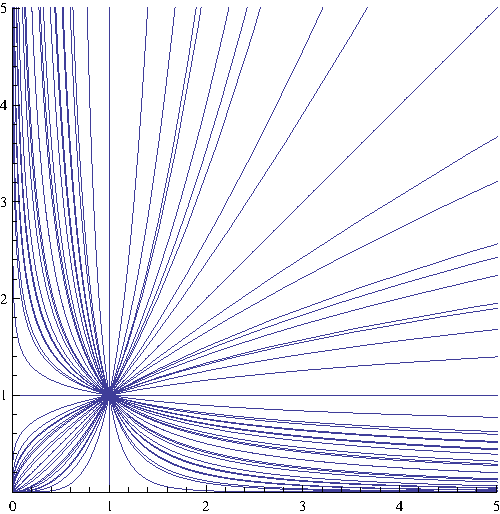
\includegraphics[width=2in]{03-Patterns/support/logspace-picture}

	\item The 3rd and 4th axioms for scalar multiplication fail. 
%	(M1) $k[(a,b)+(c,d)] = k(a+c,b+d) = (2k(a+c),2k(b+d)) = (2ka+2kc,2kb+2kd) = (2ka,2kb)+(2kc,2kd)=k(a,b)+k(c,d)$.
%	(M2) $(j+k)(a,b) = (2(j+k)a,2(j+k)b) = (2ja + 2ka,2jb+2kb) = (2ja,2jb)+(2ka,2kb) = j(a,b)+k(a,b)$.
	(M3) $j(k(a,b)) = j(2ka,2kb)=(2j2ka,2j2kb)=jk(2a,2b)$ instead of $jk(a,b)$.
	(M4) $1(a,b) = (2a,2b)\neq (a,b)$.
	
	
	\item
\begin{enumerate}
	\item 
	Distribution across scalar multiplication fails:  
	$(j+k)(a,b) = (a,(j+k)b) = (a,jb+kb)$ whereas $j(a,b)+k(a,b) = (a,jb)+(a,kb) = (2a,(j+k)b)$ 
	(notice that $a$ is doubled if we multiply first before adding).
	\item  
	Vector addition is not commutative. $(a,b)+(c,d) = (a+c,b)$ while $(c,d)+(a,b) = (a+c,d)$ 
	(the second components are not the same, $b\neq d$.
\end{enumerate}


	\item 
\begin{enumerate}
	\item  Distribution across scalar multiplication fails.
	(M2) $(j+k)(a,b) = ((j+k)^2a,(j+k)b)$ whereas $j(a,b)+k(a,b) = (j^2a,jb)+(k^2a,b) = ((j^2+k^2)a,(j+k)b)$, and $j^2+k^2\neq (j+k)^2$.
	\item  
	Vector addition is not commutative. $(a,b)+(c,d) = (a,d)$ while $(c,d)+(a,b) = (c,b)$.
	
\end{enumerate}


\end{enumerate}



\item \textbf{Vector Subspaces:} 
See chapter 4 problems 13-15, 45-46. Complete at least 13, 15, 46.

\begin{enumerate}
	\item 
		\begin{enumerate}
			\item Yes.  It contains zero, the sum of any two vectors on the $y$ axis is on the $y$ axis, and any scalar multiple of a vector on the $y$ axis is still on the $y$ axis.  The span of $(0,1)$ is the $y$ axis.
			\item No. The zero vector is not on the positive $x$ axis.
			\item No. You cannot times vectors by negative scalars, so it's not closed under scalar multiplication.
			\item Yes. It is the span of $(1,3)$. Lines through the origin are vector subspaces.
			\item No. The line does not contain the zero vector.  It doesn't pass through the origin.
			\item No. It does contain the origin, and is closed under scalar multiplication, but not under vector addition.  The sum $(1,0)+(0,1)=(1,1)$ is not on either axis.
			\item No. Not closed under scalar multiplication. The product $4(1/2,0) = (2,0)$ is not in the set.
		\end{enumerate}


	\item Use theorem \ref{thm subspace iff closed}.
	(1) The zero function is continuous, so zero is in the set. 
	(2) The sum of two continuous functions is a continuous function, so the set is closed under addition.
	(3) A constant times a continuous function is still continuous, so the set is closed under scalar multiplication.
	
	\item Use theorem \ref{thm subspace iff closed}.
	(1) The zero function is a polynomial, so zero is in the set. 
	(2) The sum of two polynomials is a polynomial, so the set is closed under addition.
	(3) A constant times a polynomial is a polynomial, so the set is closed under scalar multiplication.
	
	
	\item 
\begin{enumerate}
	\item 
	(1) The zero function is said to be in the set, so zero is in the set. 
	(2) The sum of two polynomials of degree three must be a polynomial of degree 3 or less, so the set is closed under addition.
	(3) Multiplying a polynomial by a nonzero constant does not change the degree, so the set is closed under scalar multiplication.

	\item The span of the polynomials $\{1,x,x^2,x^3\}$ is $P_3(x)$.  
\end{enumerate}

	\item Let $V$ be the set of 3 by 3 upper triangular matrices.  Show that $V$ is a subspace of the vector space $M_{33}$ of 3 by 3 matrices in 2 ways:
\begin{enumerate}
	\item 
	(1) The zero matrix is upper triangular. 
	(2) The sum of two upper triangular matrices is upper triangular, so the set is closed under addition.
	(3) Multiplying an upper triangular matrix by a constant gives an upper triangular matrix, so the set is closed under scalar multiplication.

	\item 
	The span of 
	$\begin{bmatrix}
	1&0&0\\
	0&0&0\\
	0&0&0
	\end{bmatrix}$,
	$\begin{bmatrix}
	0&1&0\\
	0&0&0\\
	0&0&0
	\end{bmatrix}$,
	$\begin{bmatrix}
	0&0&1\\
	0&0&0\\
	0&0&0
	\end{bmatrix}$,
	$\begin{bmatrix}
	0&0&0\\
	0&1&0\\
	0&0&0
	\end{bmatrix}$,
	$\begin{bmatrix}
	0&0&0\\
	0&0&1\\
	0&0&0
	\end{bmatrix}$,
	$\begin{bmatrix}
	0&0&0\\
	0&0&0\\
	0&0&1
	\end{bmatrix}$
	is the set of upper triangular matrices
  $\begin{bmatrix}
	a&b&c\\
	0&d&e\\
	0&0&f
	\end{bmatrix}$.

	
\end{enumerate}
	\item 
		\begin{enumerate}
			\item 
			Yes. Zero is a symmetric matrix. The sum of two symmetric matrices is symmetric. A constant times a symmetric matrix is symmetric.  Alternatively, the symmetric matrices 
	$\begin{bmatrix}
	a&b\\
	b&c
	\end{bmatrix}$
are spanned by 
	$\begin{bmatrix}
	1&0\\
	0&0
	\end{bmatrix}$
,
	$\begin{bmatrix}
	0&0\\
	0&1
	\end{bmatrix}$
, 
	$\begin{bmatrix}
	0&1\\
	1&0
	\end{bmatrix}$, and hence are a subspace of $M_22$.
			\item	No. The zero matrix is not invertible. 
			\item Yes. Similar to the previous problem related to 3 by 3 matrices.
		\end{enumerate}

	\item 
		\begin{enumerate}
			\item No. The zero polynomial does not have degree 2.
			\item No. The sum of two degree 2 polynomials may be lower in degree.  For example $(x^2) + (x-x^2) = x$. So this set is not closed under addition.
			\item Yes. It is spanned by $\{1,x,x^2\}$
			\item No. Similar to part (b).
		\end{enumerate}

\end{enumerate}




\item \textbf{Spans:} \label{span solutions} \hypertarget{span solutions target}{\hyperlink{span problems target}{(problems link)}}

\begin{enumerate}
	\item 
All but the third have the same row space. The rref of these matrices has the same nonzero rows.


	\item 
All but the third have the same column space. The rref of the transpose of each matrix has the same nonzero rows.

	\item 
		\begin{enumerate}
			\item Yes. The rref is the identity.
			\item No. Only 2 independent columns. Column 3 has coordinates $(3,-1)$.
			\item No. You need at least 3 vectors to span $P_2(x)$.
			\item Yes. There are 3 independent vectors.  The 4th column has coordinates $(1,-1,2)$.
			\item No. Only 2 independent vectors. The coordinates of column 3 are $(1,-1)$, column 4 $(1,2)$.
		\end{enumerate}

	\item 
		\begin{enumerate}
			\item No. You need at least 4 vectors.
			\item Yes.
			\item No. The third polynomial is the sum of the first 2.  There are only 3 independent vectors. 
		\end{enumerate}

	\item 
		\begin{enumerate}
\item 
Yes.

\item 
No.

\item 
No.

\item 
Yes.

		\end{enumerate}
		
\item \textbf{Basis and Dimension:} 
		
\end{enumerate}












\end{enumerate}
\end{multicols}





\restoregeometry
\chapter{Linear Transformations}

This chapter covers the following ideas. The purpose of this chapter is to extend the notion of functions between numbers to functions between vector spaces.  We'll see that vector subspaces related to these functions can help us solve many problems we have been looking at in previous chapters.


\begin{enumerate}

\item Construct graphical displays of linear transformations.  Graphically explain how to see eigenvalues, eigenvectors, and determinants from these visualizations, as well as when an inverse transformation exists.
\item Know the vocabulary of functions: domain, range, image, inverse image, kernel, injective (one-to-one), surjective (onto), and bijective. 
\item Define linear transformation, and give examples involving both finite and infinite dimensional vector spaces. 
Show that every linear transformation between finite dimensional vector spaces can be represented by a matrix in relation to the standard basis vectors.
\item Describe the column space, null space, and eigenspaces of a matrix. Show that these spaces are vector spaces. 
\item Show that every solution to the linear equation $T(\vec x)=\vec b$ can be written in the form $\vec x = \vec x_p+\vec x_h$, where $\vec x_p$ is a particular solution and $\vec x_h$ is a solution to the homogeneous equation $T(\vec x)=\vec 0$.
\item Explain what it means to compose linear transformations (both algebraically and graphically). Then show how to decompose a matrix as the product of elementary matrices, and use this decomposition (through row reduction) to compute the determinants of large matrices. 


\end{enumerate}


\section{Matrix Transformations}


In this section, we'll explore how matrices transform (reshape, move) the plane and space. 
In the next section we will use this geometric idea to define linear transformations. 
We'll then show that every matrix represents a linear transformation, and that every linear transformation (between finite dimensional vector spaces) can be represented as a matrix.  
The study of linear algebra is really the study of linear transformations between vector spaces. 
Since linear transformations can be represented as matrices, we began our study with matrices.

\subsection{Square Matrices}

Let's start by illustrating how a square matrix $A$ transform a vector $\vec x$ into another vector $A\vec x$. 
For what follows, we will think of the matrix $A$ acting on a vector $\vec x$ to product a transformed vector $A\vec x$.
For a 2 by 2 matrix such as $A = \begin{bmatrix}\cl{2\\0}&\cl{1\\3}\end{bmatrix}$, the columns of $A$ tell us where to map $\vec e_1 = (1,0)$ and $\vec e_2=(0,1)$.
The product $A\vec e_1 = (2,0)$ is the first column of $A$ and $A \vec e_2 = (1,3)$ is the second column. 
Every other vector $(x,y)$ in 2D is transformed in a similar fashion by considering the product 
\begin{align*}
A\begin{bmatrix}x\\y\end{bmatrix} 
&=A\left(x\begin{bmatrix}1\\0\end{bmatrix}+ 
y\begin{bmatrix}0\\1\end{bmatrix}\right) &\text{write in terms of basis}\\
A\begin{bmatrix}x\\y\end{bmatrix} 
&=A\begin{bmatrix}x\\0\end{bmatrix}+ 
A\begin{bmatrix}0\\y\end{bmatrix} &\text{distribute across addition}\\
&=xA\begin{bmatrix}1\\0\end{bmatrix}+ 
yA\begin{bmatrix}0\\1\end{bmatrix} &\text{pull scalars out front}\\
&=xA\vec e_1+yA\vec e_2.
\end{align*}
From the previous computation, once we know where $(1,0)$ and $(0,1)$ are transformed, we can transform every other vector by just using this information. Once know what the matrix $A$ does to a basis of $\mathbb{R}^2$, we know what the matrix does to every other vector in $\mathbb{R}^2$, because every other vector is a linear combination of these basis vectors.



We'll illustrate this transformation with 2D plots (see figure \ref{matrix transformation example}). We draw the vectors $(1,0),(0,1)$ and their images $(2,0),(1,3)$.  The unit square transforms into a parallelogram. The matrix transforms a triangle into a new triangle, a circle into an ellipse, and a heart into a slanted heart. One key observation is that the matrix transforms lines to lines, which is why we call it a linear transformation. 

\begin{figure}
\begin{center}
\begin{tikzpicture}[inner sep=0mm]
\node (middle) {\begin{tabular}{c}
Matrix\\
$\begin{bmatrix}\cl{2\\0}&\cl{1\\3}\end{bmatrix}$\\
Determinant\\
6\\
Eigenvalues\\
2,3\\
Eigenvectors\\
(1,0), (1,1)
\end{tabular}};
\node (B) [left=of middle,xshift=1cm] {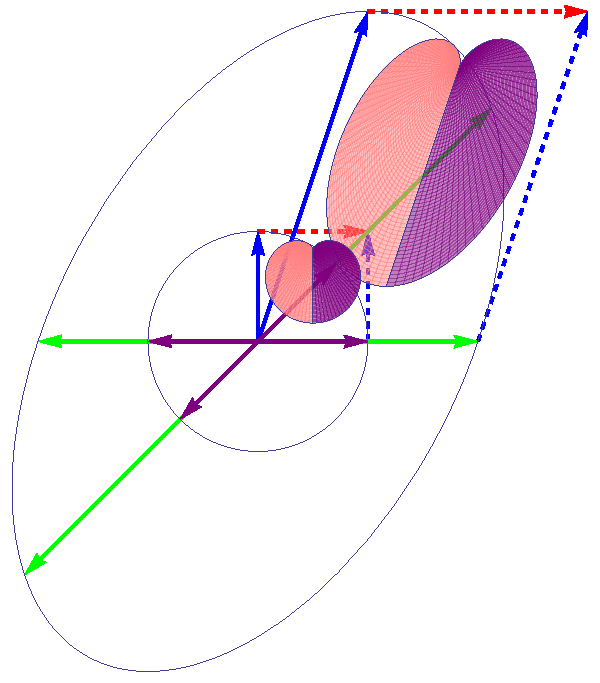
\includegraphics[height=2in]{04-Linear-Transformations/support/LT1b}};
\node (A) [left=of B,xshift=1cm] {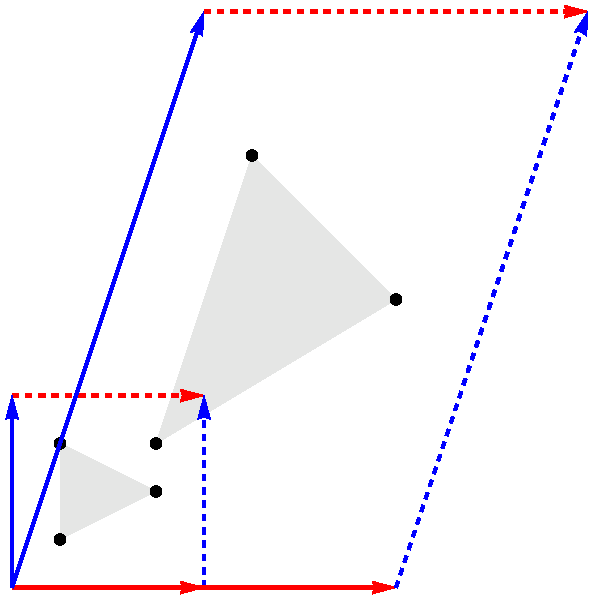
\includegraphics[height=2in]{04-Linear-Transformations/support/LT1}};
\end{tikzpicture}
\end{center}

\caption{{
Two visualizations of a transformation. 
	Matrix transformations map (see left) lines to lines, triangles to triangles, boxes to parallelograms, and (see right) circles to ellipses.		
	Every other point is transformed in a similar fashion (the heart maps to a slanted heart). 
	The determinant measures the increase in area (the parallelogram has 6 times the area of the box, the ellipse has 6 times the area of the circle).	
	Eigenvectors tell you the directions in which the transformation moves points radially outwards. 
	Eigenvalues tell you how much outward stretching occurs in the eigenvector directions. 
}}
\label{matrix transformation example}
\end{figure}

The eigenvectors of this transformation tell us the directions in which things are transformed radially outwards 
(hence $A\vec x = \lambda \vec x$ means that the vector $\vec x$ is just stretched outward by the factor $\lambda$).  
The determinant tells us how much area (or volume) is stretched by, and if the transformation involved a flip. 
The determinant is the product of the eigenvalues, so an outward stretch of 2 in one direction followed by an outward stretch of 3 in another direction should result in increasing the area by a factor of (2)(3)=6 (see figure \ref{matrix transformation example}). 
If the determinant of our transformation is zero, then in some direction the transformation squashes things flat.
Once an object has been squashed flat, it is impossible to invert this transformation (which is why there is no inverse when the determinant is zero). 
Time for some more examples.



\begin{example}\label{details for four}

Figure \ref{four matrix transformations} illustrates the transformations given by  the four matrices 
$$A = 
\begin{bmatrix}
3&1\\1&3
\end{bmatrix}
,
B = 
\begin{bmatrix}
-1&-1\\-3&1
\end{bmatrix}
,
C = 
\begin{bmatrix}
1&1\\1&-1
\end{bmatrix}
,
D = 
\begin{bmatrix}
1&1\\-1&1
\end{bmatrix}
.$$ 

For $A$, the matrix has two positive eigenvalues. The transformation pushes everything outwards.  In the $(1,1)$ directions, lengths are multiplied by 4.  In the $(-1,1)$ direction, lengths are multiplied by 2.  This results in the area increasing by a factor of 8.  Notice that the eigenvector directions provide the major and minor axes for the ellipse.  This is always true when the matrix is symmetric.

For $B$, the matrix has a positive and negative eigenvalue.  The determinant is negative which is because the image was flipped over in the transformation.  Area is increased by a factor of 4.  The matrix is not symmetric, which is why the eigenvector directions are not the major and minor axes of the transformed ellipse.

We'll look at $C$ and $D$ simultaneously.  The difference between these two matrices is that the columns have been interchanged. Interchanging the columns results in a flip, which causes the determinant to switch signs. The area increase for both is 2.  The eigenvalues of $D$ are complex, which means there is no direction in which points are transformed radially outwards - every point is rotated some amount by this transformation.      

\newcommand{\myvfplotheight}{1.8in}
\begin{figure}
\begin{tikzpicture}

\node (symmetric) {\begin{tabular}{c}
Matrix\\
$\begin{bmatrix}\cl{3\\1}&\cl{1\\3}\end{bmatrix}$\\
Determinant\\
8\\
Eigenvalues\\
$4,2$\\
Eigenvectors\\
$(1,1), (-1,1)$
\end{tabular}};
\node [right=of symmetric] {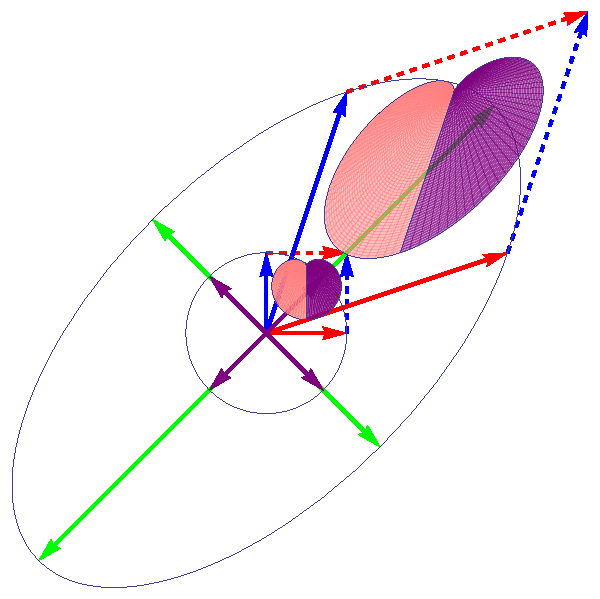
\includegraphics[height=\myvfplotheight]{04-Linear-Transformations/support/LTsymmetricb}};
\node [left=of symmetric] {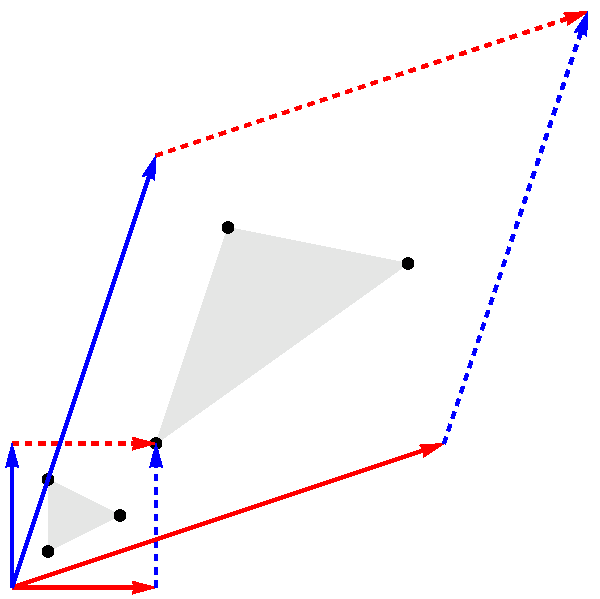
\includegraphics[height=\myvfplotheight]{04-Linear-Transformations/support/LTsymmetrica}};


\node (negative) [below=of symmetric] {\begin{tabular}{c}
Matrix\\
$\begin{bmatrix}\cl{-1\\-3}&\cl{-1\\1}\end{bmatrix}$\\
Determinant\\
-4\\
Eigenvalues\\
$-2,2$\\
Eigenvectors\\
$(1,1), (-1,3)$
\end{tabular}};
\node [right=of negative] {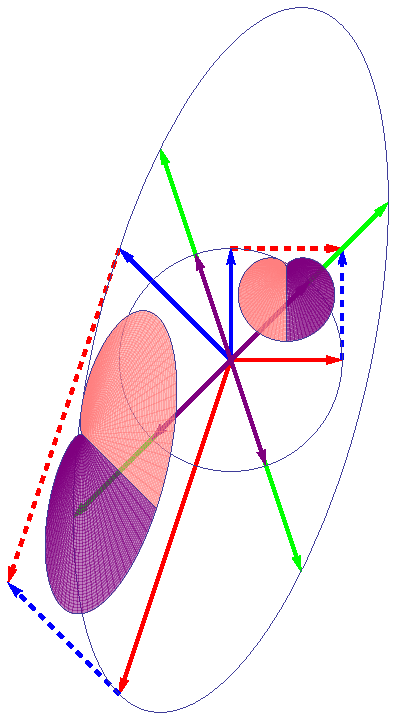
\includegraphics[height=\myvfplotheight]{04-Linear-Transformations/support/LTnegativeb}};
\node [left=of negative] {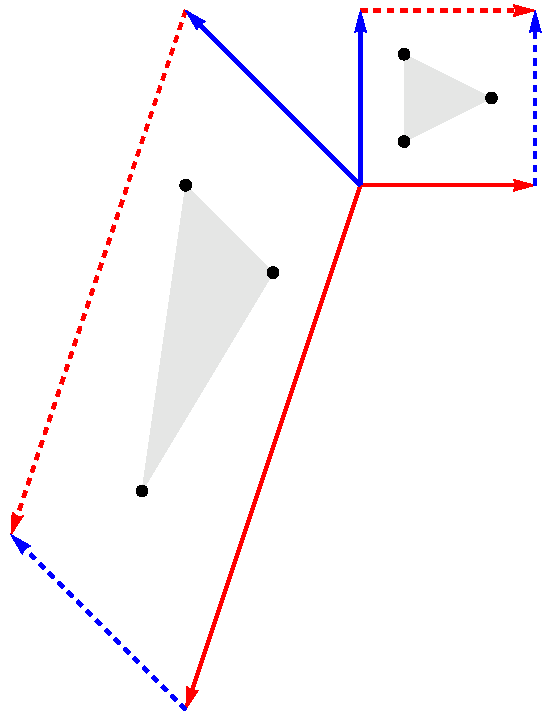
\includegraphics[height=\myvfplotheight]{04-Linear-Transformations/support/LTnegativea}};


\node (irrational) [below=of negative] {\begin{tabular}{c}
Matrix\\
$\begin{bmatrix}\cl{1\\1}&\cl{1\\-1}\end{bmatrix}$\\
Determinant\\
-2\\
Eigenvalues\\
$-\sqrt{2},\sqrt{2}$\\
Eigenvectors\\
$(1-\sqrt2,1), (1+\sqrt2,1)$
\end{tabular}};
\node [right=of irrational] {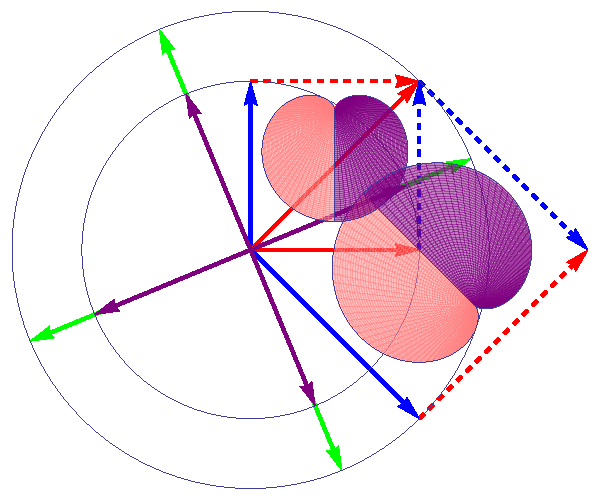
\includegraphics[height=\myvfplotheight]{04-Linear-Transformations/support/LTirrationalb}};
\node [left=of irrational] {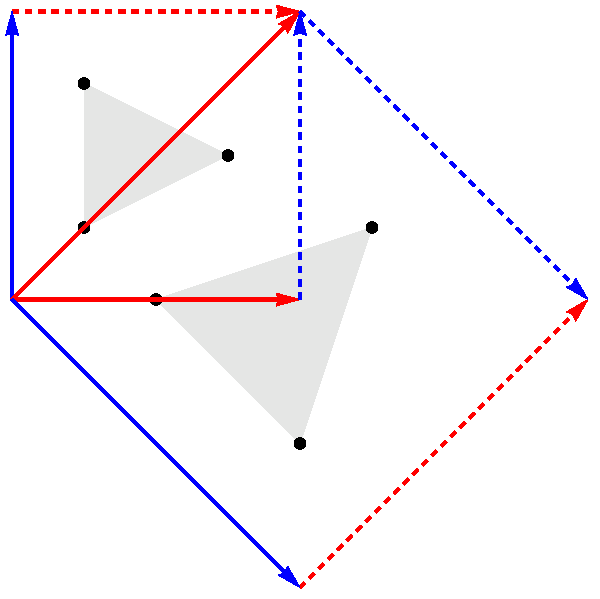
\includegraphics[height=\myvfplotheight]{04-Linear-Transformations/support/LTirrationala}};

\node (complex) [below=of irrational] {\begin{tabular}{c}
Matrix\\
$\begin{bmatrix}\cl{1\\-1}&\cl{1\\1}\end{bmatrix}$\\
Determinant\\
2\\
Eigenvalues\\
$1+i,1-i$\\
Eigenvectors\\
$(-i,1), (i,1)$
\end{tabular}};
\node [right=of complex] {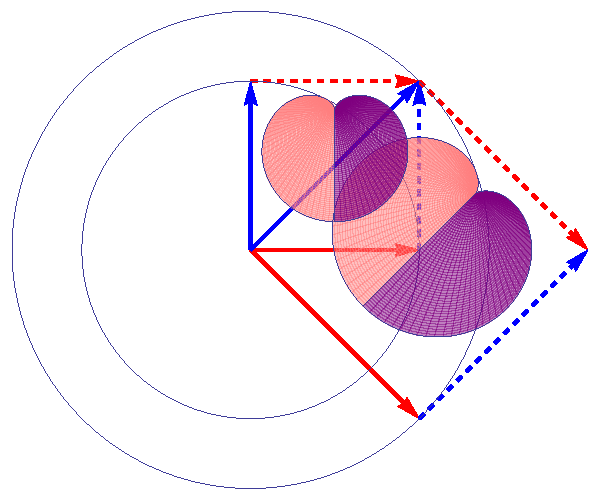
\includegraphics[height=\myvfplotheight]{04-Linear-Transformations/support/LTcomplexb}};
\node [left=of complex] {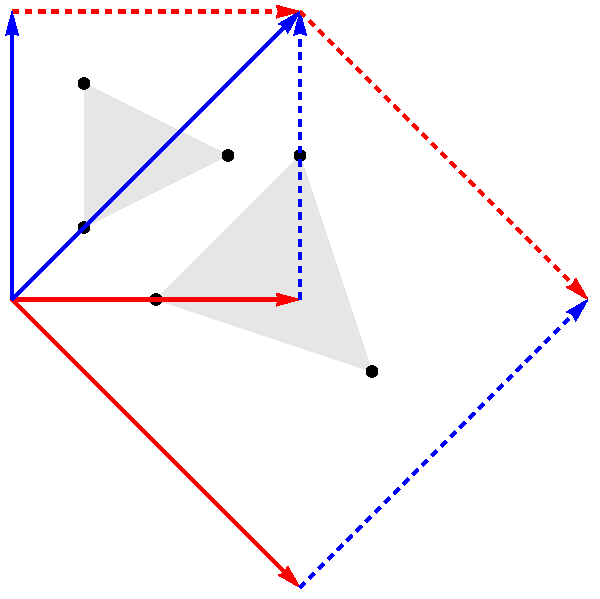
\includegraphics[height=\myvfplotheight]{04-Linear-Transformations/support/LTcomplexa}};

\end{tikzpicture}
\caption{Four 2D transformations. See example \ref{details for four} for details. In the picture on the right, the purple vectors are eigenvectors of length 1, where the green vectors have been scaled by the eigenvalue.
}
\label{four matrix transformations}
\end{figure}
\end{example}

\marginpar{PDF documents utilize vector graphics so that you can zoom in on the image as far as you want and still have smooth edges on your text. I have created this text using vector graphics where possible so that you can zoom in on any image and still see a high quality image.} Vector graphics (such as those used in PDF documents) utilize linear transformations to create images.  
When you zoom in to view a PDF document, the computer redraws all the text so that every corner is still smooth.  
Scanners and digital cameras store their data as pixels instead of as vectors. 
If you scan a document and then zoom in, the document appears grainy.  
Vector graphics prevent pixel errors from occurring as each time you zoom in the computer knows exactly how to transform text so that smooth edges occur. 


\subsubsection{3 by 3 Matrices}

Let's now look at some visualization of 3D transformations. The ideas are similar to what happens in 2D, we just add an additional dimension. This adds another eigenvector direction, and instead of talking about an increase in area, we now talk about an increase in volume. 

\begin{example}\label{3d transformation example}
Consider the two matrices 
. Figure \ref{matrix transformation 3d example} illustrates the transformations resulting from the two matrices $\bm{ 2 & 0 & 0 \\ 1 & 2 & 1 \\ 0 & 1 & 2}$
and 
$\bm{ 0 & 0 & -1 \\ 0 & -3 & 0 \\ -2 & 0 & 0}$ in two different ways.  The first image shows how to transform a 3D surface.  The second illustration shows how to transform a sphere into an ellipsoid, and it also includes the eigenvector directions. You can log on to Sage to view more images and rotate the images to get a better view of what each transformation does. 

Both matrices have determinant 6, which means that in both cases the volume of objects is increased by 6 through the transformation.  The first transformation stretches objects by 1 in the direction $(0,-1,1)$, by 2 in the direction $(-1,0,1)$, and by 3 in the direction $(0,1,1)$.  The second transformation has two directions in which a reflection occurs (the product of two negatives results in a positive determinant).  The amount of each stretch, together with the direction, is listed in the figure.


\begin{figure}
\begin{center}
\begin{tikzpicture}
\node (middle) {\begin{tabular}{c}
Matrix\\
$\bm{ 2 & 0 & 0 \\ 1 & 2 & 1 \\ 0 & 1 & 2}$\\
Determinant\\
6\\
Eigenvalues\\
$1,2,3$\\
Eigenvectors\\
$(0,-1,1)$\\$(-1,0,1)$\\$(0,1,1)$
\end{tabular}};
\node (middle2) [below=of middle] {\begin{tabular}{c}
Matrix\\
$\bm{ 0 & 0 & -1 \\ 0 & -3 & 0 \\ -2 & 0 & 0}$\\
Determinant\\
6\\
Eigenvalues\\
$-3,-\sqrt{2},\sqrt 2$\\
Eigenvectors\\
$(0,1,0)$\\$(\sqrt2/2,0,1)$\\$(-\sqrt2/2,0,1)$
\end{tabular}};
\node  [left=of middle] {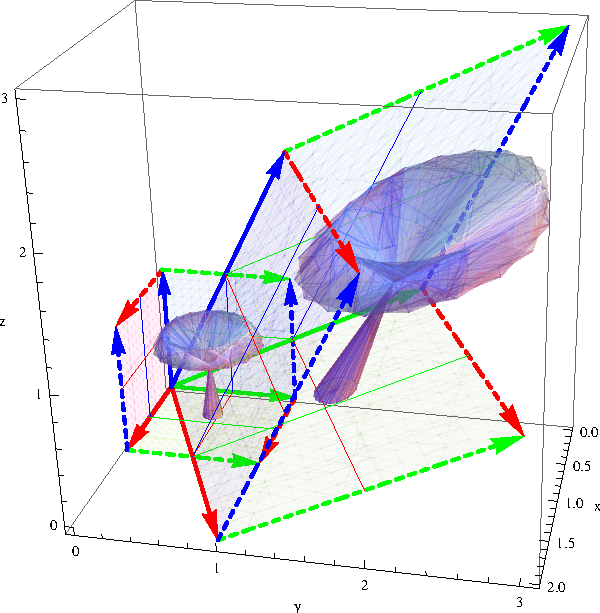
\includegraphics[width=2in]{04-Linear-Transformations/support/LT3da}};
\node  [right=of middle]  {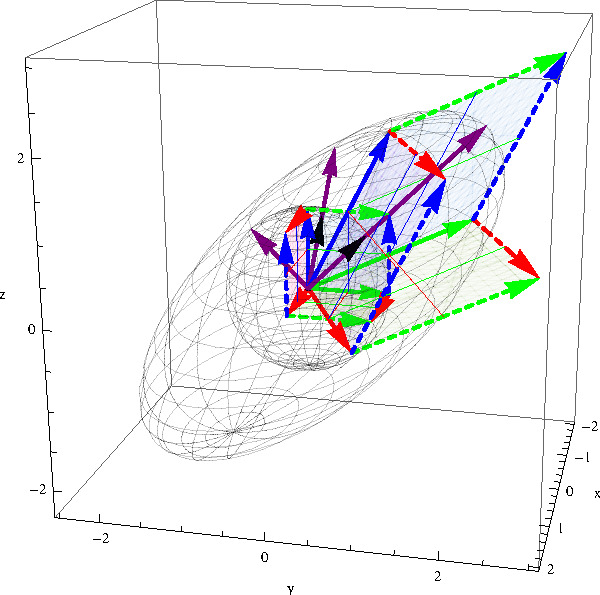
\includegraphics[width=2in]{04-Linear-Transformations/support/LT3db}};
\node  [left=of middle2]{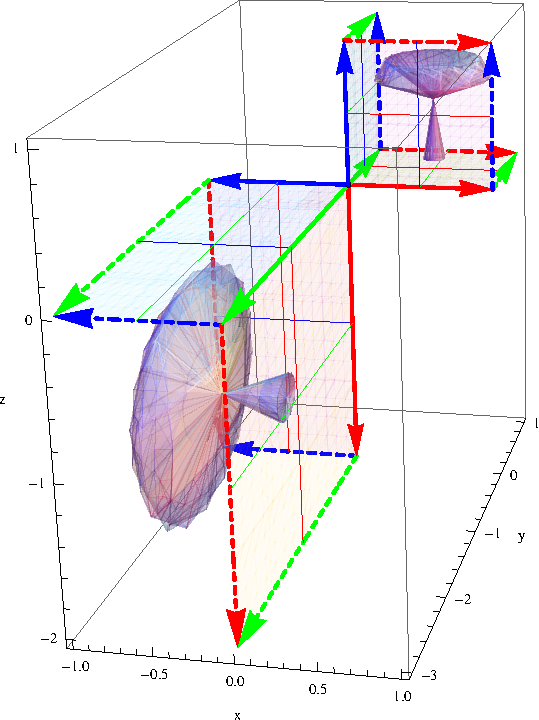
\includegraphics[width=2in]{04-Linear-Transformations/support/LT3d2a}};
\node  [right=of middle2] {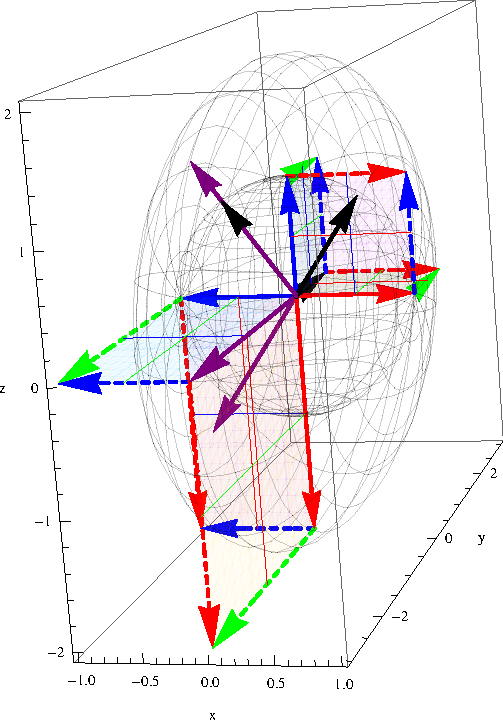
\includegraphics[width=2in]{04-Linear-Transformations/support/LT3d2b}};
\end{tikzpicture}
\end{center}

\caption{{
Two 3D transformations. See example \ref{3d transformation example} for details. In the picture on the right, the black vectors are eigenvectors of length 1, where the purple vectors have been scaled by the eigenvalue.}}
\label{matrix transformation 3d example}
\end{figure}




\end{example}

\subsubsection{Singular Matrices - Not Invertible}

In all the examples above, we have been looking at square matrices where the determinant is nonzero.  When the determinant is zero, the matrix does not have an inverse and we say the matrix is singular.  This means that the columns are linearly dependent, which means that when we construct a visualization of the transformation, we should see multiple columns overlapping. The next example illustrates this in both 2D and 3D.  

\begin{example}
For the matrix 
$A=\bm{1&-2\\-1&2}$, we map $(1,0)$ to $(1,-1)$ and $(0,1)$ to $(-2,2)$. Both vectors lie on the same line.
We obtain the two visualizations below. \marginpar{When the determinant is zero, a 2D transformation takes the entire plane to a line. The column space is the line onto which the transformation maps.}
\begin{center}
\includegraphics[height=2in]{04-Linear-Transformations/support/LTsingular2da}
\includegraphics[height=2in]{04-Linear-Transformations/support/LTsingular2db}
\end{center}
Notice that every vector, in addition to $(1,0)$ and $(0,1)$, is mapped onto this same line.  The column space of $A$ is precisely the line given by the span of $(-1,1)$. The column space corresponds directly with the line onto which everything is mapped. Because $\det A = 0$, we know that $\lambda=0$ is an eigenvalue. The corresponding eigenvector $(2,1)$ is drawn in the image on the right. This eigenvector is found by solving $A\vec x = 0$, which means that the set of solutions is the null space. \marginpar{The null space of $A$ is precisely the set of vectors which get squashed to $\vec 0$ by $A$.} Every vector on the line containing $(2,1)$ is transformed to the origin (so in this direction we are squashing an entire line to a point).  Because this transformation squashes two dimension onto a line, it is impossible to invert the transformation (hence no inverse exists).

\end{example}
\begin{example}
For the matrix 
$A=\bm{ 0 & 1 & -1 \\ -1 & 0 & 1 \\ 1 & -1 & 0}$, we map 
the vector $(1,0,0)$ to $(0,-1,1)$, 
the vector $(0,1,0)$ to $(1,0,-1)$, and 
the vector $(0,0,1)$ to $(-1,1,0)$. These three images lie on the same plane (since the determinant is zero).  We obtain two visualizations below. \marginpar{When the determinant is zero, a 3D transformation takes the all of space to a plane (if the rank is 2) or a line (if the rank is 1). The column space is precisely the subspace of $\mathbb{R}^3$ onto which the transformation squashes things.}
\begin{center}
\includegraphics[height=2in]{04-Linear-Transformations/support/LTsingular3da}
\includegraphics[height=2in]{04-Linear-Transformations/support/LTsingular3db}
\end{center}
Notice that every vector  is mapped onto the same plane containing column vectors of $A$. 
The column space of $A$ is precisely the plane onto which everything is mapped. 
The eigenvector corresponding to $\lambda =0$ is $(1,1,1)$, found by solving $A\vec x=\vec 0$, i.e. finding the null space.
This eigenvector is drawn in the image on the right.  
Anything which lies on the line containing $(1,1,1)$ is also transformed to the origin, so in this direction we are squashing an entire line to a point. 
Because this transformation squashes three dimension onto a 2D plane, it is impossible to invert the transformation (hence $A$ has no inverse). 
Non invertible square transformations always involve squashing a dimension.

  
\end{example}

In summary, if the determinant is nonzero, then the transformation maps all of 2D to all of 2D, or all of 3D to all of 3D.  
If the determinant is zero, then the the transformation maps 2D onto a subspace of 2D (a line), or 3D onto a subspace of 3D (a plane or line).  
In all cases, the column space of the matrix is precisely the space onto which the transformation maps vectors. 
If the matrix has a zero determinant, then the column space is not all of 3D and helps us understand where to map vectors.  

\subsection{Non Square Matrices}

Every example we have looked at till now involved either a 2 by 2 or 3 by 3 matrix.  
In this case we were mapping the plane to the plane, or space to space. 
What kind of transformation does a non square matrix represent, and what use would it be?  
Every time we watch television, we are viewing a 3D world that has been represented to us in a 2D way.  
This is an example of a transformation which takes us from 3D to 2D (often written $\mathbb{R}^3\to \mathbb{R}^2$).  
Computer animators (movies and computer games) start by constructing a 3D model of a world, and then use matrix transformations to map this 3D world into a 2D presentation for viewing. 
Projecting a 2D image into 3D (written $\mathbb{R}^2\to \mathbb{R}^3$) requires a transformation from 2D to 3D. 

How does the size of the matrix determine the kind of transformation.  
For an $m$ by $n$ matrix $A$, the matrix product $A\vec x = \vec b$ requires that $\vec x$ be $n$ dimensional, and $\vec b$ be $m$ dimensional.  
So when you put in vectors of size $n$, you get out vectors of size $m$.  
This meas that a matrix $A_{mn}$ results in a linear transformation $A:\mathbb{R}^n\to\mathbb{R}^m$. 
Did you notice the change in order from $mn$ to $n\to m$? 
The size of the matrix tells us first the dimension of the outputs and then the dimension of the inputs.
Let's look at two more examples.  
Then we'll be ready to generalize the patterns we've observed into a general theory about linear transformations.  

\begin{example}
Let's look at the two transformations given by the matrices
$A=\bm{0&1\\1&0\\1&1}$ and 
$B=\bm{-2&-1&-1\\1&2&-1}$.
The first transformation requires that we input 2D vectors and returns 3D vectors. To graph this transformation, we notice that multiplying $A$ by the vectors $(1,0)$ and $(0,1)$ returns the two columns of $A$.  So in the $xy$ plane we draw the unit square, and in 3D we graph the parallelogram formed by the two columns.  This is illustrated below. Notice that the unit circle becomes an ellipse in the plane spanned by the columns of $A$.  Again we see that all the output vectors are drawn in the column space of $A$.
\begin{center}
\includegraphics[width=\marginparwidth]{04-Linear-Transformations/support/LT2dto3d}
\end{center}

The transformation given by $B$ requires that we input a 3D vector to obtain a 2D vector.  We graph the unit cube in 3D and graph the columns of $A$ in the $xy$ plane. In this transformation, we are squashing a dimension out of the problem. This is the kind of transformation used to cast shadows in 3D graphics, as well as to present a 2D image of 3D objects for viewing on a screen. 
\begin{center}
\includegraphics[height=2in]{04-Linear-Transformations/support/LT3dto2d}
\end{center}


\end{example}






\section{What is a Linear Transformation?}

\subsection{General Function Notation and Vocabulary}
Let's start with a review of function notation from beginning algebra. 
A function $y=f(x)$ is a rule which assigns to each input $x$ from the domain a value $y$ from the range. 
Notationally we may write $f:D\to R$ to represent the function as a map from $D$ (the domain) to $R$ (the range).  
The sets $D$ and $R$ in previous classes have normally been the set of real numbers. 
Before we proceed to work with functions between vector spaces, we need to build some vocabulary. 
We now consider functions (maps or transformations) from any set $D$ to any set $R$.
\begin{definition}
\begin{itemize}
	\item Any mapping which assigns to each element of $D$ exactly one element of $R$ is called a function. We write $f:D\to R$ to emphasis the domain $D$ and range $R$ (also called the codomain). 

	\item The image of an element $x\in D$ is the value $y\in R$ such that $f(x)=y$. We can write $x\mapsto y$ (read $x$ maps to $y$) to illustrate the idea that the input $x$ transforms into the output $y$ through this function. 

	\item The image of $f$, written $\im f=f(D)$, is the set of $y\in R$ which are the image of some $x\in D$. In set notation we write $\im f = \{y\in R\ |\ f(x)=y$ for some $x\in D\}$.

	\item The preimage of $y\in R$, written $f^{-1}(y)$, is the set of all $x\in D$ such that $f(x)=y$. 
	
	\item We say a function is one-to-one, or injective, if $f(x_1)=f(x_2)$ implies that $x_1=x_2$ (every $y$ value in the image has only one $x$ value which maps to it).  
	\item We say a function is onto, or surjective, if every $y\in R$ is the image of some $x\in D$ (the function hits every $y$ value in the range).  
	\item We say a function is bijective if $f$ is both one-to-one and onto (both injective and surjective). In this case we define $f^{-1}$ to be the function which inverts $f$. 
	\item The composition of two functions $f:A\to B$ and $g:B\to C$ is a new map $g\circ f:A\to C$ defined by $(g\circ f)=g(f(a))$. Notice that in order to compose two maps, the image of $f$ must be a subset of the domain of $g$.  

\end{itemize}
\end{definition}


\begin{example}
Consider the sets $D=\{A,B,C\}, R_1=\{1,3,9\},$ and $R_2=\{1,3,7,9\}$.
\begin{enumerate}
	\item If we define $f(A)=1,f(B)=9,f(C)=3$, then $f:D\to R_1$ is a function.  The image of $B$ is $9$, so we write $B\mapsto 9$. The image of $f$ is $f(D)=\{1,3,9\}$, so $f$ is onto. The preimage of $3$ is $f^{-1}(3)=C$. This map $f:D\to R_1$ is injective and surjective, hence it has an inverse. However if I change the range to $R_2$ instead of $R_1$, then the function is not surjective (onto) because 7 is not the image of any value in $D$ (the preimage of $7$ is empty).
	\item If we define $f(A)=1,f(A)=9,f(C)=3$, then $f:D\to R_1$ is not a function. For one, $f(B)$ is not defined. In addition, $f(A)$ takes on two values, $A\mapsto 1,9$ which is not allowed.
	\item If we define $f(A)=1,f(B)=3,f(C)=3$, then $f$ is a function.  The image of both $B$ and $C$ is $9$ so the preimage of $3$ is $f^{-1}(3)=\{B,C\}$, which means the map is not injective (as $f(B)=f(C)$, but $B\neq C$).
	\item If we define $f:A\to R_1$ by $f(A)=1,f(B)=3,f(C)=9$, and we define $g:R_1\to R_2$ by $g(1),g(3)=3,g(9)=7$, then the composite function $g\circ f$ satisfies $g(f(A))=g(1)=1$, $g(f(B))=g(3)=3$, and $g(f(C))=g(9)=7$. The composite is injective, but not surjective (it misses 9). 
\end{enumerate}
\end{example}

\subsection{Linear Transformations}
One of the main topics in linear algebra is the study of special types of functions, called linear transformations (or linear mappings) where the domain and codomain (range) are both vector spaces.  All of the transformations resulting from matrices in the first section are linear transformations.  The following definition is a result of noticing the patterns which arose from the examples above.  
\begin{definition}[Linear Transformation]
We call a function $T:V\to W$ between vector spaces $V$ and $W$ linear (or called a linear transformation) if both of the following criteria are satisfied:
\begin{enumerate}
	\item $T(\vec v_1+\vec v_2)=T(\vec v_1)+T(\vec v_2)$ for every $\vec v_1,\vec v_2\in V$
	\item $T(c\vec v)=cT(\vec v)$ for every scalar $c$ and vector $\vec v\in V$.
\end{enumerate}
We say that $T$ preserves vector addition and scalar multiplication.
\end{definition}
\marginpar{If $T$ is linear, then the transform of a linear combination is the linear combination of the transforms: $$T\left(\sum_{i=1}^n c_i\vec v_i\right) = \sum_{i=1}^n T(c_i\vec v_i).$$}
A linear transformation is a function between vector spaces in which you can perform vector addition and scalar multiplication  either before or after applying the function. 
If a function is linear, then repeated application of the definition shows that $$T(c_1\vec v_1+\cdots +c_n\vec v_n) = c_1T(\vec v_1)+\cdots +c_nT(\vec v_n).$$ Linear combinations of vectors becomes linear combinations of the images of each vector when using a linear transformation.  \marginpar{Once you know what a linear transformation does to a basis, you know what it does to all of the space.}

 In particular, this means that if you know the value of the linear transformation at each point of a basis for $V$, then every other value of the function is known as well by writing every other vector as a linear combination of basis vectors. 
\begin{example}
Let's start by illustrating what a linear transformation is not. We'll show that the function $f(x) = 2x+1$, $g(x)=x^2$, and $h(x,y)=(x+y,xy)$ are not linear transformations.
\begin{enumerate}
	\item The function $f(x)=2x+1$ (whose graph is a line which does not pass through the origin) is not linear because
	 $$f(x+y)=2(x+y)+1 = 2x+2y+1$$ whereas if we transform each point and then sum we obtain $$f(x)+f(y)=2x+1+2y+1 = 2x+2y+2.$$
	 Because $f(x+y)\neq f(x)+f(y)$, this function is not linear. 
	 \marginpar{Linear transformations map $\vec 0$ to $\vec 0$.}
	 Linear transformations always map the zero vector to the zero vectors (lines through the origin are linear transformations).
	\item The function $g(x)=x^2$ (a parabola) is not linear because $$g(x+y)=(x+y)^2 = x^2+2xy+y^2 = g(x)+g(y)+2xy \neq g(x)+g(y).$$ 
	Alternatively, we could also look at scalar multiplication to show this function is not linear, because $g(2x) = 4x^2$ whereas $2g(x) = 2x^2$ and so $g(2x)\neq 2g(x)$. 
	Raising variables to powers other than 1 results in nonlinear maps.
	\item The function $h(x,y)=(x+y,xy)$ is not linear. We can show this by looking at an example, rather than using variables. 
	We compute $f(1,1)=(2,1)$ and $f(2(1,1)) = f(2,2)=(4,4)$, but $2f(1,1) = (4,2)$. 
	So we have shown by example that $f(2\vec x)\neq 2f(\vec x)$. 
	\marginpar{You can show a function is not linear by providing one example.}
	The map does not preserve scalar multiplication. 
	The component $xy$ is the problem here. In general, multiplying variables together creates nonlinear functions.  
\end{enumerate}
\end{example}

Now let's look at some examples of linear transformations. 
In each example, we will formally show that the function is linear by showing that it preserves both vector addition and scalar multiplication.  
The first 3 examples are crucial, while the last 3 represent ideas explored more in future classes where vector spaces of infinite dimension are studied. 
Practical applications to the telecommunications industry, jpeg, mp3, and many more require knowledge about infinite dimensional vector spaces.  
In this class we will focus on transformations between finite dimensional vector spaces.

\begin{example}
\marginpar{Lines through origin $y=mx$ are linear transformations from $\mathbb{R}$ to $\mathbb{R}$.}
The function $T(x)=4x$ is linear because (1) $T(x+y) = 4(x+y) = 4x+4y = T(x)+T(y)$ (the map preserves vector addition) and (2) $T(cx)=4(cx)=c(4x)=cT(x)$ (the map preserves scalar multiplication).
\end{example}

The first example showed that any line through the origin, $y=mx$, is a linear transformation. In the next two examples, we'll show that any function of the form $\vec y = M\vec x$ is a linear transformation as well.  The reason we use the letter $m$ to represent slope is because the $m$ stands for ``matrix,'' where we replace $x$ and $y$ with vectors. Linear transformations are really just extensions of the simple line $y=mx$ to higher dimensions. The slope becomes a matrix, while the variables become vectors.

\begin{example} \label{ltex matrix1}
The function $T:\mathbb{R}^2\to \mathbb{R}^2$ defined by $T(x,y)=(2x+3y,x-y)$ is linear.  To show this, we check that $T$ preserves both vector addition and scalar multiplication.
\begin{enumerate}
	\item $T((x,y)+(s,t)) = T((x+s,y+t))=(2(x+s)+3(y+t),(x+s)-(y+t)) = (2x+3y,x-y)+ (2s+3t,s-t) = T(x,y)+T(s,t)$, hence the map preserves vector addition. 
	\item $T(c(x,y))= T(cx,cy) = (2cx+3cy,cx-cy)=c(2x+3y,x-y)=cT(x,y)$, hence the map preserves scalar multiplication.
\end{enumerate}
 We can write this function in matrix form as 
	$$T(x,y)=(2x+3y,x-y)=\begin{bmatrix}2&3\\ 1&-1\end{bmatrix}\begin{bmatrix}x\\y\end{bmatrix}.$$ 	
	\marginpar{The columns of the matrix are the images of the basis vectors (1,0) and (0,1). }
	Notice that $T(1,0)=(2,1)$ is the first column and $T(0,1)=(3,-1)$ is the second column.

\end{example}

\begin{example}\label{ltex matrix2}
Now let's work with a vector space other than $\mathbb{R}^n$. 
Let $V=P_2(x)$ be the set of polynomials of degree 2 or less, together with the zero polynomial.  
The derivative function $D:P_2(x)\to P_2(x)$ defined by $D(a+bx+cx^2)=b+2cx$ is a linear transformation. 
\begin{enumerate}
	\item The derivative preserves vector addition because $(f+g)'=f'+g'$ by the sum rule for derivatives.
	\item The derivative preserves scalar multiplication becuse $(cf)'=c(f)'$ by the constant multiple rule for derivatives.
\end{enumerate}
The vectors $\{1,x,x^2\}$ are the standard basis vectors for $P_2(x)$. 
Relative to this standard basis, the coordinates of $a+bx+cx^2 = a(1,0,0)+b(0,1,0)+c(0,0,1)$ are just $(a,b,c)$. 
We can then rewrite the derivative transformation in coordinate form as $D(a,b,c) = (b,2c,0)$. 
In matrix form, we write
 $$D(a,b,c)
 =(b,2c,0)
 =\begin{bmatrix}0&1&0\\0&0&2\\0&0&0\end{bmatrix}\begin{bmatrix}a\\b\\c\end{bmatrix}.$$ 
 Notice that $D(1,0,0)=(0,0,0)$ is the first column, $D(0,1,0)=(1,0,0)$ is the second column, and $D(0,0,1)=(0,2,0)$ is the third column. 
 \marginpar{The columns of our matrix are the coordinates of the images of our basis vectors}
 In general, the columns of our matrix will be the coordinates of the images of the standard basis vectors.
\end{example}

\begin{example}
Let $V=P(x)$ be the set of polynomials, an infinite dimensional vector space with basis $\{1,x,x^2,x^3,\ldots\}$.  
The derivative transformation $D:P(x)\to P(x)$ is a linear transformation because of the sum rule and constant multiple rule for derivatives (just as in the last example). 
For those of you who have had math 113, Taylor polynomials and Taylor series are all related to this vector space and transformations on it.
\end{example}

\begin{example}
Let $V$ be the set of functions that are infinitely differentiable on the entire real number line (so $e^x, \sin x, \cos x, x^2$, etc. are examples). 
The derivative transformation $D:V\to V$ defined by $D(f) = f'$ is a linear transformation on this space (by the same arguments as the previous example). Notice that you input a function $f$ and get out a function $f'$, so this map takes vectors in $V$ to vectors in $V$.  This space is infinite dimensional, and a basis for this space is so large that we say it is uncountable (those of you headed on to more math classes will study the difference between countably infinite and uncountably infinite in future classes).

Let $T:V\to \mathbb{R}$ be the integral transformation, defined by $T(f)=\int_0^1 f(x)dx$.  This transformation takes a function $f$ and returns a real number by integrating from $[0,1]$.  To show this function is linear, we check 
\begin{enumerate}
	\item $\ds \int_0^1 f(x)+g(x)dx=\int_0^1 f(x)dx+\int_0^1 g(x)dx$, so $T(f+g)= T(f)+T(g)$ (vector addition is preserved), 
	\item $\ds \int_0^1 cf(x)dx =c\int_0^1 f(x)dx$, so $T(cf) = cT(f)$ (scalar multipilcation is preserved).
\end{enumerate}
The derivative and integral are both examples of linear transformations that you have studied before. The difference is that the derivative returns functions, while the integral returns numbers.  The codomain is $V$ for derivatives, and the vector space $\mathbb{R}$ for integrals.  
In real analysis, these ideas are explored in greater depth and become foundational tools for understanding finance, economics, and more.
\end{example}

\begin{example}
Let $V$ be the set of infinitely differentiable function on the real line.  Let $$L(y(x))=y^{\prime\prime}(x)-2xy^\prime(x)+3x^2 y(x)$$ be the differential operator which takes multiple derivatives of $y$ and combines them together by multiplying by functions of $x$.  This is a linear transformation $L:V\to V$ because 
\begin{enumerate}
	\item $L(y_1+y_2)=(y_1+y_2)^{\prime\prime}-2x(y_1+y_2)^\prime+3x^2 (y_1+y_2) = (y_1^{\prime\prime}-2xy_1^\prime+3x^2 y_1) +(y_2^{\prime\prime}-2xy_2^\prime+3x^2 y_2)=L(y_1)+L(y_2)$, and
	\item $T(cy)=(cy)^{\prime\prime}-2x(cy)^\prime+3x^2 (cy) = c(y^{\prime\prime}-2xy^\prime+3x^2 y)=cT(y)$.
\end{enumerate}
 We use transformations like $L$ to find solutions to differential equations, and show that the set of solutions is a vector space. These ideas are studied more in differential equations, engineering, and physics, and become the foundational tool for understanding mechanical systems, electrical circuits, radio waves, signal processing, and more.  
\end{example}






\subsection{Standard Matrix Representation}
Every matrix we have studied this semester represents a linear transformation. 
To verify that every matrix represents a linear transformation, we need to show that matrices preserve vector addition and scalar multiplication. We have already seen that $A(\vec x+\vec y) = A\vec x+A\vec y$ and $A(c\vec x)=c(A\vec x)$, which is precisely what is meant by matrix multiplication preserves vector addition and scalar multiplication.  

Conversely, every linear transformation (between finite dimensional vector spaces) can be expressed in matrix form $T(\vec x)=A\vec x$ for some matrix $A$.
Examples \ref{ltex matrix1} and \ref{ltex matrix2} illustrate how to find the matrix $A$ relative to the standard basis. . 
To find this matrix, we start by computing the image of each standard basis vector, i.e. $$T(1,0,\ldots,0),T(0,1,\ldots,0), \ldots,T(0,0,\ldots,1).$$ We then place these vectors in the columns of a matrix.  This matrix $A$ is called the standard matrix representation of the linear transformation. We use the word ``standard'' because are using the standard basis vectors to give the coordinates of each vector.  The next two units explore using different basis vectors to describe linear transformations. Time for some examples.

\begin{example}
Let's find the standard matrix representation of the linear transformation $$T(x,y,z,w)=(2x+3y-4z,x+y-w,z+2x-5w).$$ We start by computing the values at each of the 4 basis vectors  $$T(1,0,0,0)=(2,1,2),T(0,1,0,0)=(3,1,0),T(0,0,1,0)=(-4,0,1),T(0,0,0,1)=(0,-1,-5).$$ 
We now place these vectors into the columns of a matrix which gives the standard matrix representation
$$T(x,y,z,w)=A\vec x=
\begin{bmatrix}
2&3&-4&0\\
1&1&0 &-1\\
2&0&1 &-5
\end{bmatrix}
\begin{bmatrix}
x\\
y\\
z\\
w
\end{bmatrix}.$$ 
The matrix $A$ is called the standard matrix representation of $T$. 
Notice that we input 4D vectors (hence 4 columns) and get out 3D vectors (hence 3 rows).  
\marginpar{The number of rows is the dimension of the range. The number of columns is the dimension of the domain.} 
Each input dimension gets a column, and each output dimension gets a row.   
\end{example}

Sometimes a linear transformation is described in words.  Examples include things like ``rotate everything 30 degrees'' or ``find the shadow of this object if the sun is located at ...''  In such a case, you can create the standard matrix representation of the transformation by asking where each basis vector is sent.  Here is an example.

\begin{example}
Let's rotate an object in the plane counterclockwise by 90 degrees. 
How do we obtain the standard matrix representation of this transformation? 
We find what happens to the standard basis vectors. 
We'll let $T(x,y)$ be the linear transformation which rotates counterclockwise by 90 degrees, we see that $T(1,0)=(0,1)$ and $T(0,1)=(-1,0)$.  
This means the standard matrix representation of $T$ is 
$$\begin{bmatrix}
\cos \pi/2&\cos\pi\\
\sin\pi/2&\sin\pi
\end{bmatrix}=\begin{bmatrix}0&-1\\1&0\end{bmatrix}. \quad\quad \text{(a rotation of 90 degrees)}$$

If instead we want to rotate counterclockwise by 30 degrees ($\pi/6$ radians)  then we compute 
$T(1,0) = (\cos \pi/6, \sin \pi/6) = (\sqrt3/2,1/2)$ (the values on the unit circle at $\pi/6$)  and 
$T(0,1) = (\cos 2\pi/3, \sin 2\pi/3) = (-1/2,\sqrt3/2) $ (the values on the unit circle at $\pi/2+\pi/6 = 2\pi/3$). 
This means the standard matrix representation of $T$ is 
\marginpar{
\includegraphics[width=\marginparwidth]{04-Linear-Transformations/support/LTrotate30}

A 30 degree rotation.}
$$
\begin{bmatrix}
\cos \pi/6&\cos(\pi/2+\pi/6)\\
\sin\pi/6&\sin(\pi/2+\pi/6)
\end{bmatrix}
=\begin{bmatrix}\sqrt3/2&1/2\\-1/2&\sqrt3/2\end{bmatrix}. \quad\quad \text{(a rotation of 30 degrees)}$$  

\end{example}

Let's generalize the pattern we've seen above to include rotations through any angle. We can write the image of the second basis vector above in terms of trig function at $\theta$, instead of at $\pi/2+\theta$, if we recall that $\cos(\pi/2+\theta) = -\sin(theta)$ and $\sin(\pi/2+\theta) = \cos(theta)$ (these identities just say that shifting cosine left $\pi/2$ gives negative sine, and shifting sine left $\pi/2$ gives cosine.  
We ca now write the standard matrix representation of a rotation through $\theta$ degrees as
$$
\begin{bmatrix}
\cos \theta&\cos(\pi/2+\theta)\\
\sin \theta&\sin(\pi/2+\theta)
\end{bmatrix}
=
\begin{bmatrix}
\cos \theta&-\sin\theta\\
\sin \theta&\cos\theta
\end{bmatrix}.
\quad\quad \text{(a rotation of $\theta$ radians)}
$$




Sometimes we are able to extract from a problem information about how a transformation changes vectors other than the standard basis vectors.  When this occurs, provided we know that the transformation does to a basis, we can still find the standard representation. It just requires a little more work. Let's look at an example. 

\begin{example}
Suppose we know that $T(x,y)$ is a linear transformation from $\mathbb{R}^2$ to $\mathbb{R}^3$ and we know that $T(1,1)=(3,0,5)$ and $T(2,0)=(1,-2,0)$. Because we haven't computed the transformation at $(1,0)$ and $(0,1)$
We don't know $A$ yet, but we do know that 
$$
A\begin{bmatrix}1\\1\end{bmatrix} = \begin{bmatrix}3\\0\\5\end{bmatrix}, 
A\begin{bmatrix}2\\0\end{bmatrix} = \begin{bmatrix}1\\-2\\0\end{bmatrix},\quad \text{ or  } \quad
A\begin{bmatrix}1&2\\1&0\end{bmatrix} = \begin{bmatrix}3&1\\0&-2\\5&0\end{bmatrix}
$$  
The vectors $(1,1)$ and $(2,0)$ are linearly independent, so they form a basis for $\mathbb{R}^2$. The matrix formed by placing these vectors in columns, $\begin{bmatrix}1&2\\1&0\end{bmatrix}$, is an invertible matrix since the columns are independent. Since it is invertible, we can multiply both sides of our equation on the right by this inverse to obtain $$A= \begin{bmatrix}3&1\\0&-2\\5&0\end{bmatrix}\begin{bmatrix}1&2\\1&0\end{bmatrix}^{-1} = \begin{bmatrix}3&1\\0&-2\\5&0\end{bmatrix}\begin{bmatrix}0&1\\1/2&-1/2\end{bmatrix} =\begin{bmatrix}1/2&5/2\\-1&1\\0&5\end{bmatrix}.$$ 
We found the standard matrix representation by using the inverse of basis vectors given. We can check that our matrix $A$ is correct by computing the matrix product 
$$\begin{bmatrix}1/2&5/2\\-1&1\\0&5\end{bmatrix}
\begin{bmatrix}1&2\\1&0\end{bmatrix} 
= \begin{bmatrix}3&1\\0&-2\\5&0\end{bmatrix}$$ to show that $T(1,1)=(3,0,5)$ and $T(2,0)=(1,-2,0)$ as required.  We also know now that $T(1,0) = (1/2,-1,0)$ and $T(0,1)=(5/2,1,5)$, so we know the images of the standard basis vectors. 
\end{example}
 
In general, when you know what a transformation does to any basis of the domain, you can use this to find the standard matrix by multiplying on the right by an inverse.  
Schaum's outlines writes out the equations and then solves them (which is equivalent to using an inverse). 
Let's focus on the fact that the inverse is the key tool needed to understand the transformation.




  
\section{Subspaces From Linear Transformations}

In the first section where we graphed matrix transformations, we noticed that the column space of the matrix was related to the possible outputs of the transformation. We also saw that the null space of the matrix told us precisely which vectors in the domain were mapped to the origin.  These two spaces associated with matrices are important subspaces related to general linear transformations.  Because a linear transformation could have a domain or range which is infinite dimensional, we need a new word to talk about these subspaces of transformations, even when no matrix exists to represent the transformation.  The new words are image and kernel. Here are the formal definitions.

\begin{definition}
Let $T:V\to W$ be a linear transformation.  
\begin{enumerate}
	\item The image of $T$ (written $\im T$) is the set of all values in $W$ which are the image of some $\vec v$ in $V$. 
	Symbolically we write $$\im T = \{\vec y\in W \ | \ T(\vec x)=\vec y \text{ for some $\vec x\in V$}\}.$$ 
	\item The kernel of $T$ (written $\ker T$) is the set of all values in $W$ whose image is $\vec 0$ in $W$. 
	Symbolically we write $$\ker T = \{\vec x\in V \ | \ T(\vec x)=\vec 0\}.$$
\end{enumerate}
\end{definition}

Linear transformations may not always be represented with matrices. However, when you can represent a transformation with a matrix, these new words are precisely the same as the column space and null space of a matrix.  Let's formalize this pattern into a theorem.
\begin{theorem}
If $T:V\to W$ is a linear transformation between finite dimensional vector space, and the standard matrix representation of $T$ is $A$, 
\begin{enumerate}
	\item the column space of $A$ equals the image of $T$ and 
	\item the null space of $A$ equals the kernel of $T$.
\end{enumerate}
\end{theorem}

We already know that the column space and null space of a matrix are vector subspaces.  This should also be true of the image and kernel of the transformation. Remember, to show that something is a subspace we must show that it contains $\vec 0$ and is closed under vector addition and scalar multiplication.  Let's first state our next theorem, and then verify that it is indeed true. 

\begin{theorem}
Let $T:V\to W$ be a linear transformation. 
\begin{enumerate}
	\item The image of $T$ is a vector subspace of the range (codomain) $W$. 
	\item The kernel of $T$ is a vector subspace of domain $V$.
\end{enumerate}
\end{theorem}
Notice that the image is a subspace of the range, and the kernel is  subspace of the domain. The image is the set of outputs, and the kernel is the set of inputs that map to zero. 

\begin{example}
Let's show that the image of $T$ is a vector subspace of $W$. I'll let you show that the kernel is a vector subspace of $V$ in the homework.

We have to show three things: (1) the zero vector in $W$ is in the image, (2) the image is closed under addition, and (3) the image is closed under scalar multiplication.
\begin{enumerate}
	\item We know that linear transformations map the zero vector to the zero vector.  So the image of the zero vector $\vec 0_V$ in $V$ is precisely $T(\vec 0_V) = \vec 0_W$, the zero vector in $W$.  Hence $\vec 0_W$ is in the image.
	\item We need to show that if $\vec y_1$ and $\vec y_2$ are in the image, then so is their sum.  
	Well, since $\vec y_1$ belongs to $W$, we know that $\vec y_1 = T(\vec x_1)$ for some $\vec x_1\in V$.  
	Similarly $\vec y_2 = T(\vec x_2)$ for some $\vec x_2\in V$.  
	We can now compute (since $T$ is linear and preserves addition) \marginpar{Linear transformations preserve addition. This is why the image is closed under addition.}  $$T(\vec x_1+\vec x_2) = T(\vec x_1)+T(\vec x_2) = \vec y_1+\vec y_2$$ 
	which means that the sum $\vec y_1+\vec y_2$ is the image of $\vec x_1+\vec x_2$. 
	This shows that the image is closed under vector addition.
	\item The only thing that remains is to show that if $\vec y$ is in $W$, then so is any scalar multiple of $\vec y$. Since $\vec y\in W$, we know there is some $\vec x\in V$ such that $T(\vec x)=\vec y$. 
	If $c$ is any constant, then we can compute (since $T$ is linear and preserves scalar multiplication) 
	\marginpar{Linear transformations preserve scalar multiplication. This is why the image is closed under scalar multiplication.}
	$$T(c\vec x) = cT(\vec x) = c\vec y$$ which means that $c\vec y$ is the image of $c\vec x$.
	This shows that the image is closed under scalar multiplication.
	
\end{enumerate}

Your job in the homework will be to show that the kernel of a linear transformation is a vector subspace of the domain $V$.

\end{example}

Now that we know the image and kernel of a transformation are vector subspaces, we can look for spanning sets, bases, and find the dimension of these spaces. We used the word ``rank'' as the dimension of the column space, but have not yet given a name to the dimension of the null space.  Here are some more definitions.

\begin{definition} 
Let $T:V\to W$ be a linear transformation. 
The dimension of the image of $T$ is called the rank of $T$ (just as the rank is the dimension of the column space).
The dimension of the kernel of $T$ is called the nullity of $T$ (and we use the same word for the null space). 

\end{definition}

Now that we have some words to describe the dimensions of the image and kernel, we can state one of the key theorems which relates these two subspaces.  A basis for the column space of a matrix $A$ is simply the pivot columns of $A$. We find a basis for the null space by solving for all the variables in terms of the free variables, which means that each free variable contributes a vector to the basis of the null space.  Since the free variables correspond to non pivot columns, and the column space corresponds to pivot columns, we see that the sum of the dimensions of the column space and null space must always equal the number of columns.  

\begin{theorem}[The Rank-Nullity Theorem]
Let $T:V\to W$ be a linear transformation between finite dimensional vector spaces, whose standard matrix representation is $A$.  Then 
\begin{enumerate}
	\item The rank of $T$ is the number of pivot columns of $A$. 
	\item The nullity of $T$ is the number of non pivot columns of $A$. 
	\item The rank of $T$ plus the nullity of $T$ is always equal to the dimension of $V$. 
\end{enumerate}
\end{theorem}

Notice that the third item does not refer at all to the matrix $A$.  The third fact is true provide that only $V$ is finite dimensional (and hence has no standard matrix representation). Time for some examples.


\begin{example}
Consider the linear transformation $T:{\mathbb{R}}^5\to {\mathbb{R}}^6$ with standard matrix 
$$A=\begin{bmatrix}
 1 & 2 & 0 & 1 & 1 \\
 2 & -3 & -7 & -1 & 13 \\
 0 & 1 & 1 & 1 & -1 \\
 4 & 0 & -8 & 4 & 20 \\
 3 & 0 & -6 & 3 & 15 \\
 0 & 0 & 0 & 0 & 0
 \end{bmatrix} 
\xrightarrow{rref}
\begin{bmatrix}
 1 & 0 & -2 & 0 & 4 \\
 0 & 1 & 1 & 0 & -2 \\
 0 & 0 & 0 & 1 & 1 \\
 0 & 0 & 0 & 0 & 0 \\
 0 & 0 & 0 & 0 & 0 \\
 0 & 0 & 0 & 0 & 0
\end{bmatrix}.$$

The column space of $A$ is the span of the columns of $A$. 
The image $T$ is all vectors of the form $A\vec x$ - but this is the span of the columns of $A$. 
This means that the column space of $A$ and the image of $T$ are the same vector subspace of ${\mathbb{R}}^6$, the range of $T$. 
A basis for this vector subspace is the set of pivot columns $$\{(1, 2, 0, 4, 3, 0), (2, -3, 1, 0, 0, 0), (1, -1, 1, 4, 3, 0)\},$$ so the column space has dimension 3. The rank of $A$ and the rank of $T$ are both 3.

To find the null space of $A$, and hence the kernel of $T$, we solve the equation $A\vec x=0$.  The 3rd and 5th columns correspond to the free variables.  We can write the solution as 
$$
\begin{matrix}
x_1-2x_3+4x_5=0\\
x_2+1x_3-2x_5=0\\
x_3=x_3\\
x_4+x_5=0\\
x_5=x_5
\end{matrix}
\Rightarrow
\begin{matrix}
x_1=2x_3-4x_5\\
x_2=-1x_3+2x_5\\
x_3=x_3\\
x_4=-x_5\\
x_5=x_5
\end{matrix}
\Rightarrow
\begin{bmatrix}
x_1\\
x_2\\
x_3\\
x_4\\
x_5
\end{bmatrix}=
x_3
\begin{bmatrix}
2\\
-1\\
1\\
0\\
0
\end{bmatrix}+
x_5
\begin{bmatrix}
-4\\
2\\
0\\
-1\\
1
\end{bmatrix}.
$$
We see that the null space is the span of the vectors $$\{(2,-1,1,0,0),(-4,2,0,-1,1)\}.$$ 
The kernel of $T$ is a vector subspace of ${\mathbb{R}}^5$, the domain of $T$.  
The numbers in these vectors are the opposite of the numbers in the non pivot columns of rref, with a 1 or 0 placed in the spots representing the free variables.  
The reason we negate all the numbers is that we have to subtract these numbers from both sides of the first equation to solve for each variable in terms of the the free variables.  
The nullity of $T$ is 2 (the number of free variables). 
The rank plus the nullity equals $3+2=5$, the dimension of the domain (or number of columns).
\end{example}


%The null space of a transformation can help us understand how the transformation modifies space.  If the null space is empty, then no vectors will be mapped to zero except for zero itself.  This means that the transformation will map lines to line, planes to planes, 3D spaces to 3D spaces, etc.  In this case, we say the linear transformation is nonsingular. If the domain and range have the same dimension, then the transformation will have an inverse. If however the transformation has a nonzero kernel (null space is not just zero), then in some direction things the dimension is reduced. We call the transformation singular, and it cannot have an inverse. A entire line gets mapped to a point, or an entire plane gets mapped to a line.  The dimension of the kernel helps us understand how much ``squashing'' is happening with our transformation. Use the Maple illustration code to see what happens with some transformations which are singular.

\subsection{Solutions to Systems and the Kernel}

The kernel arises from solving the equation $T(\vec x)=\vec 0$.  Can we use the kernel to help us solve the equation $T(\vec x)=\vec b$?  The answer is amazingly yes. The key lies in the fact that if both $\vec x_1$ and $\vec x_2$ are solutions to $T(\vec x)=\vec b$, then their difference $\vec x_1-\vec x_2$ is in the kernel of $T$.  This follows immediately from the computation $T(\vec x_1-\vec x_2)=T(\vec x_1)-T(\vec x_2)=\vec b-\vec b=\vec 0$. This means that $\vec x_2=\vec x_2+\vec x_h$ where $\vec x_h$ is some vector in the kernel of $T$. Here is the general idea.
\begin{theorem}
Let $T$ be a linear transformation. Consider the nonhomogeneous equation $T(\vec x)=\vec b$.
If $\vec x_p$ is one particular solution to the equation $T(\vec x)=\vec b$, then every solution can be written in the form $\vec x = \vec x_p+\vec x_h$, where $\vec x_h$ is a solution to the corresponding homogeneous equation $T(\vec x)=\vec 0$.  In other words, every solution to the nonhomogeneous equation is found by first finding a particular solution $\vec x_p$, and then adding to it every vector in the kernel.  
\end{theorem} 
This theorem is a key tool used to solve differential equations.  Once you know one solution, you can find every other solution by just adding to that solution the entire kernel (null space). This makes the kernel an extremely useful subspace to know.

\begin{example}
Suppose that a system of equations reduces to the matrix below.
\begin{center}
\begin{tabular}{cc}
$\begin{bmatrix}[ccccc|c] 0&1&0&2&0&0\\0&0&1&3&0&1\\0&0&0&0&1&4\\0&0&0&0&0&0\end{bmatrix}$
&
$\begin{bmatrix}x_1\\x_2\\x_3\\x_4\\x_5\end{bmatrix} 
= \begin{bmatrix}0\\0\\1\\0\\4\end{bmatrix}
+x_1\begin{bmatrix}1\\0\\0\\0\\0\end{bmatrix}
+x_4\begin{bmatrix}0\\-2\\-3\\1\\0\end{bmatrix}$
\end{tabular}
\end{center} 
A particular solution to this system is $\vec x_p=(0,0,1,0,4)$ (obtained by letting the free variables $x_1$ and $x_4$ both be zero).  The null space is the span of the vectors $(1,0,0,0,0)$ and $(0,-2,-3,1,0)$. Notice that every solution to the system can be written in the form $\vec x_p +\vec x_h$, where $\vec x_h$ is a vector in the null space.
\end{example}
 
\subsection{Eigenspaces are Null Spaces}
We have already notice in the first section that the eigenvectors of a matrix tell us the directions in which a transformation pushes points radially outwards.  These directions provide us a line (vector subspace) in which all transforming is done radially outwards (or inwards if the eigenvalues are less than one in magnitude).  Recall that corresponding to each eigenvalue is an infinite collection of eigenvectors. By definition, the zero vector is not an eigenvector, hence the set of eigenvectors cannot be a vector subspace.  However, if we include the zero vector, we obtain a vector space. We now make some formal definitions.

\begin{definition}[Eigenspaces]
If $\lambda$ is an eigenvalue of a matrix $A$, then the set of vectors $E_\lambda = \{\vec x | \ A\vec x = \lambda \vec x\}$ (the eigenvectors together with zero) is called the eigenspace of $A$ corresponding to $\lambda$. 

We say that $\lambda$ is an eigenvalue of a linear transformation $T:V\to V$ (notice the domain and range are the same) if 
$T(\vec x)=\lambda \vec x$ for some nonzero $\vec x$, called an eigenvector of $T$ corresponding to $\lambda$. 
If $\lambda$ is an eigenvalue of $T$, then the set of vectors $E_\lambda = \{\vec x | \ T(\vec x) = \lambda \vec x\}$ (the eigenvectors together with zero) is called the eigenspace of $T$ corresponding to $\lambda$. 
\end{definition}
We find eigenvectors of a matrix by solving $(A-\lambda I)\vec x = \vec 0$ which means that the eigenspace $E_\lambda$ is precisely the null space of $(A-\lambda I)$.  Because the eigenspace is a null space, we know that it is a vector space.

%Another important subspace which occurs when considering a square matrix is the eigenspace of an eigenvector.  If we pick a single eigenvalue $\lambda$ and add $\vec 0$ to the set of eigenvectors, then this space is a subspace of the domain. This is because if $\vec x_1$ and $\vec x_2$ are both eigenvectors, then $A(\vec x_1+\vec x_2) = A\vec x_1+A\vec x_2 = \lambda\vec x_1+\lambda\vec x_2 = \lambda(\vec x_1+\vec x_2)$, which means $\vec x_1+\vec x_2$ is an eigenvector as well.  Similarly, $A(c\vec x_1) = c(\lambda\vec x_1)=\lambda (c\vec x_1)$, which means $c\vec x_1$ is an eigenvector as well. This shows that each eigenspace of $A$ (one for each eigenvalue) is a vector subspace of the domain. Any vector in this eigenspace will be transformed radially from the origin when you draw the transformation.  If the eigenvalue is zero, then the eigenspace will be part of the null space.

An important fact is that eigenvectors corresponding to different eigenvalues will always be linearly independent.  The full proof of this fact requires knowledge of the Vandermonde matrix, and is studied in graduate mathematics. We can discuss why this works if we consider only 2 eigenvectors.  Suppose $\vec x_1,\vec x_2$ correspond to distinct eigenvalues $\lambda_1,\lambda_2$.  Suppose in addition that $\vec x_1,\vec x_2$ are linearly dependent, which means one is a linear combination of the other $\vec x_1=c\vec x_2$.  Multiplying both sides by $A$ gives $\lambda_1 \vec x_1 = c\lambda_2\vec x_2 = \lambda_2 (c\vec x_2) = \lambda_2\vec x_1.$ This means that $\lambda_1=\lambda_2$, contrary to our assumption. Hence the two vectors must be linearly independent.

\subsection{Casting Shadows using the Null Space}

The null space of a matrix tells us the directions which get mapped to zero.  When the sun shines down on you during the afternoon, it casts a shadow on the ground.  Suppose you are positioned at the origin standing with your head up along the $z$ axis.  The sun lies with its center on a unique line through the origin, so we can pick a basis vector $(x,y,z)$ to describe the position of the sun.  As the sun casts shadows upon the ground (the $xy$ plane), all of the points along the line to the sun get mapped to the origin.  Hence, this line from the origin to the sun is precisely the null space of some matrix (there are in fact infinitely many matrices with this null space). We need to find a matrix that maps $(1,0,0)$ to $(1,0)$, maps $(0,1,0)$ to $(0,1)$ and maps $(x,y,z)$ to $(0,0)$. Computer graphic artists use this fact to cast shadows. Once we know a basis for the null space, we can create a matrix that has the null space we desire, and then transform every other point in 3D onto the plane in 2D by using this matrix.

\begin{example}
Suppose that the sun is positioned on a line containing the vector $(2,1,4)$.  
We seek a transformation that has this vector as a basis for the kernel.  
Because we're mapping from 3D onto the $xy$ plane, we need a $2$ by $3$ matrix. 
Divide every component by $4$ (to get a 1 in the $z$ component). The vector $(1/2,1/4,1)$ looks a lot like the vectors we obtain by having a free variable $z$.  The null space is all linear combinations of this vector, so we write $$\bm{x\\y\\z} = z\bm{1/2\\1/4\\1}. $$ We now have two equations $x=1/2 z$ and $y=1/4z$, or $x-\frac12 z=0$ and $y-\frac14 z=0$.  The matrix $A$ we need is precisely $$A=\bm{1&0&-1/2\\0&1&-1/4},$$ obtained by writing the coefficient matrix for the two equations. 
\marginpar{
\includegraphics[width=\marginparwidth]{04-Linear-Transformations/support/LTshadow}

Knowing the null space is sufficient to cast shadows onto the $xy$ plane.
}
Notice that $(1,0,0)$ is mapped to $(1,0)$ and $(0,1,0)$ is mapped to $(0,1)$, because when an object is already in the $xy$ plane the shadow should not move. 
The image on the right illustrates this projection. 
\end{example}


\section{Composition of Linear Transformations}
The composition of two functions $f$ and $g$ is a new function $(g\circ f)(x)$ defined by $(g\circ f)(x) = g(f(x))$.  The idea is that you input an $x$ value into $f$, and then input $f(x)$ into $g$.  The same principle applies to linear transformations.  If $S:U\to V$ and $T:V\to W$ are two linear transformations, then the composition $T\circ S:U\to W$ is defined by $T(S(\vec u))$ (where $S(\vec u)$ is a vector in $V$ which serves as an input to $T$). Let's look at an application of function composition. 

\begin{example}
If we want to rotate an object 90 degrees counterclockwise, and then mirror image the object about the $y$-axis, we can achieve this by composing two linear transformations. \marginpar{When multiple linear transformations are involved, we often use the notation $S_A$ or $T_A$ to represent the standard matrix representations.}
The linear transformation $S$ which rotates and object in the plane 90 degrees has standard matrix representation $S_A = \bm{0&-1\\1&0}$, since $S(1,0) = (0,1)$ and $S(0,1)=(-1,0)$.  
The linear transformation $T$ which mirror images objects about the $y$ axis has standard matrix representation $T_A = \bm{1&0\\0&-1}$, since $T(1,0)=(1,0)$ and $T(0,1)=(0,-1)$.  The composition $T(S(x,y))$ will first perform the rotation $S(x,y)$ and then reflect the result about the $y$ axis. We compute $S(T(x,y))$ by computing 
$$S_A\left(T_A\bm{x\\y}\right) = \bm{1&0\\0&-1}\left(\bm{0&-1\\1&0}\bm{x\\y}\right) = \bm{1&0\\0&-1}\bm{0&-1\\1&0}\bm{x\\y}. $$
Notice that function composition is precisely matrix multiplication.
\end{example}


The composition of two linear transformations has as its standard matrix representation the product of the standard matrix representations of each transformation. 
In other words, if $S: U\to V$ and $T:V\to W$ are both linear transformations with standard matrices $S_A$ and $T_A$, then $T\circ S:U \to V$ (sometimes just written $TS$) has standard matrix $(TS)_A=T_AS_A$. 
Notice that in order for this composition to make sense, then the range of $S$ and domain of $T$ must match, which means that the number of rows of $A$ must equal the number of columns of $B$ (in other words you have to be able to compute the matrix product $BA$). 
Matrix multiplication was purposefully created so that the product of matrices equals the composition of linear transformations. 

When the domain and range of a linear transformation have the same dimension, the standard matrix is a square matrix.  
In such cases, we can compute the determinant of a transformation, find the eigenvalues and eigenvectors of a transformation, and ask if the transformation is invertible. 
If the transformation $T$ is invertible with standard matrix $A$, then the standard matrix of the inverse is $A^{-1}$. Symbolically we write $T^{-1}(\vec x) = A^{-1}\vec x$. 
All of the ideas we have learned up to this point about matrices can immediately be applied to linear transformations. 


\section{Elementary Matrices and Determinants}

In the patterns chapter, theorem \ref{thm det product} stated that $|AB|=|A||B|$. The determinant of a linear transformation measures how much the transformation ``stretches'' space. If one transformation $S$ stretches space by 2 units, and another transformation $T$ stretches space by $3$ units, then applying the first transformation followed by the second should stretch space by $2\cdot 3$ units. In other words, the product of the determinants of linear transformations is precisely the determinant of the composition of the linear transformations. This is a geometric reason as to why $|AB|=|A||B|$. 
A formal proof of this fact requires breaking a matrix up into a product of elementary matrices. 
The remainder of this unit focuses on elementary matrices, which are directly related to row reduction.  
Elementary matrices will help use understand exactly how to create linear transformations by composing lots of simple transformations. 
In addition, we will discover a computationally efficient way of finding determinants of large matrices.  
Let's get started.

\begin{definition}
An elementary matrix is a matrix obtained by performing one of the following row operations to the identity matrix.
\begin{enumerate}
	\item Switch any two rows.
	\item Multiply a row by a nonzero constant.
	\item Add a multiple of one row to another.
\end{enumerate}
\end{definition}
The row operations above are precisely the operations we use to perform Gaussian elimination. 
Each row operations above is invertible as well, and the inverse is found by reversing the row operation.  
\begin{enumerate}
	\item The inverse of switching two rows is to switch the same rows again.  
	\item The inverse of multiply a row by $k$ is to multiply the same row by $1/k$.  
	\item The inverse of adding $k$ times row $i$ to row $j$ is to subtract $k$ times row $i$ from row $j$. 
\end{enumerate}
Three examples of elementary matrices follow, along with their inverses.
\begin{center}
\begin{tabular}{ccc}
Switch $R_1$ and $R_2$
&
$\begin{bmatrix}
0&1&0\\
1&0&0\\
0&0&1
\end{bmatrix}^{-1} = 
\begin{bmatrix}
0&1&0\\
1&0&0\\
0&0&1
\end{bmatrix}$
\\
Multiply $R_1$ by 2
&
$\begin{bmatrix}
2&0&0\\
0&1&0\\
0&0&1
\end{bmatrix}^{-1}=
\begin{bmatrix}
\frac{1}{2}&0&0\\
0&1&0\\
0&0&1
\end{bmatrix}
$
\\
Add $4R_3$ to $R_1$
&
$\begin{bmatrix}
1&0&4\\
0&1&0\\
0&0&1
\end{bmatrix}^{-1}=
\begin{bmatrix}
1&0&-4\\
0&1&0\\
0&0&1
\end{bmatrix}
$
\end{tabular}
\end{center}
Determinants of elementary matrices are simple as well. 
\begin{enumerate}
	\item Switching two rows results in a determinant of $-1$. You are just swapping two variables, which means that you are changing the orientation, not stretching space. 
	\item Multiplying a row by a nonzero constant results in a determinant equal to the constant. It's a triangular matrix, so just multiply the diagonal entries. Visually this can be seen as stretching space by a constant. 
	\item Adding a multiple of one row to another row results in a determinant of 1. Again we have a triangular matrix, so multiply the diagonal entries. Visually this results in a shear transformation, one in which you are pushing a part of an object in a direction without changing the volume. 
\end{enumerate}

With elementary matrices, finding inverses and determinants is easy.  We now state a key theorem which allows us to connect elementary matrices to Gaussian elimination.  

\begin{theorem}
Multiplying the matrix $A$ on the left by an elementary matrix $E$ is the same as performing on $A$ the row operation used to obtain $E$.
\end{theorem}
The reason this works is because multiplying a matrix $A$ on the left by $B$ is equivalent to computing linear combinations of the rows of $A$ using the scalars in the rows of $B$. 
(Before proceeding, try making your own example to illustrate this theorem. 
This is the key way to learn to read technical documents.)  

\begin{example}
Consider the matrix 
$A=\begin{bmatrix}
1&2&3\\
0&-1&3\\
2&-4&0
\end{bmatrix}$. 
If we multiply the matrix $A$ on the left by 
$\begin{bmatrix}
1&0&4\\
0&1&0\\
0&0&1
\end{bmatrix}$, 
we obtain 
$\begin{bmatrix}
9&-14&3\\
0&-1&3\\
2&-4&0\end{bmatrix}$. 
This is the same as adding 4 times row 3 to row 1 of $A$.  
\end{example}

\subsection{Pivotal Condensation}

We will now use elementary matrices to obtain an efficient algorithm for finding the determinant of large matrices.  This process uses row reduction, and requires keeping track of each step in the forward phase of Gaussian elimination. Numerical algorithms such as the $LU$ decomposition, or $LUP$ decomposition, use essentially the ideas presented below to compute determinants, inverses, and solve systems of equations.  We'll focus on how elementary matrices simplify the process of computing determinants.

We know that multiplying a matrix $A$ on the left by an elementary matrix $E$ is equivalent to performing a row operation on $A$. 
If $A$ reduces to the identity matrix $I$, we can repeatedly multiply by elementary matrices on the left (one matrix for each row operation) to obtain an equation $$E_n \cdots E_2E_1A=I.$$ 
Recall that the inverse of a product of matrices is found by inverting each matrix and reversing the order of the product, $(AB)^{-1} = B^{-1}A^{-1}$. 
We now multiply both sides of the equation by  
$$(E_n \cdots E_2E_1)\inv = E_1^{-1}E_2^{-1}\cdots E_n^{-1},$$ 
\marginpar{If $A$ reduces to the identity matrix, then $A$ is the product of elementary matrices.} 
and then solve for $A$ to obtain 
$$A=E_1^{-1}E_2^{-1}\cdots E_n^{-1}.$$  
Since the determinant of a product is the product of the determinants, we now have 
$$|A|=|E_1^{-1}||E_2^{-1}|\cdots |E_n^{-1}|.$$ 
If we stop the row reduction once we have obtained an upper triangular matrix $U$ (once we have put zeros in the lower left corner), then we could write $$A=E_1^{-1}E_2^{-1}\cdots E_n^{-1}U.$$  The determinant of $A$ is simply the product of the determinants of each elementary matrix multiplied by the determinant of the triangular matrix $U$, i.e. $$|A|=|E_1^{-1}||E_2^{-1}|\cdots |E_n^{-1}| |U|.$$ Let's illustrate how to find the determinant using row reduction with an example, and then state some obervations as a theorem.

\begin{example}
Consider the matrix $A=
\begin{bmatrix}
0&-1&3\\
1&2&3\\
2&-4&0
\end{bmatrix}
$.  
Let's find the determinant of $A$ using row reduction.
We reduce $A$ to an upper triangular matrix as follows:
$$\begin{bmatrix}
0&-1&3\\
1&2&3\\
2&-4&0
\end{bmatrix}
\stackrel{\xrightarrow{R_1 \leftrightarrow R_2}}{E_1}
\begin{bmatrix}
1&2&3\\
0&-1&3\\
2&-4&0
\end{bmatrix}
\stackrel{\xrightarrow{-2R_1 + R_3\to R_3}}{E_2}
\begin{bmatrix}
 1 & 2 & 3 \\
 0 & -1 & 3 \\
 0 & -8 & -6
\end{bmatrix}
\stackrel{\xrightarrow{-8R_2+R_3\to R_3}}{E_3}
\begin{bmatrix}
 1 & 2 & 3 \\
 0 & -1 & 3 \\
 0 & 0 & -30
\end{bmatrix}
$$
So far we can write this reduction process as the following product of elementary matrices.
$$E_3E_2E_1A=
\begin{bmatrix}
 1 & 0 & 0 \\
 0 & 1 & 0 \\
 0 & -8 & 1
\end{bmatrix}
\begin{bmatrix}
 1 & 0 & 0 \\
 0 & 1 & 0 \\
 -2 & 0 & 1
\end{bmatrix}
\begin{bmatrix}
 0 & 1 & 0 \\
 1 & 0 & 0 \\
 0 & 0 & 1
\end{bmatrix}
A=\begin{bmatrix}
 1 & 2 & 3 \\
 0 & -1 & 3 \\
 0 & 0 & -30
\end{bmatrix}.
$$
Solving for $A$ we obtain (remember to invert each elementary matrix and reverse the order)
$$
A=E_1^{-1}E_2^{-1}E_3^{-1}\begin{bmatrix}
 1 & 2 & 3 \\
 0 & -1 & 3 \\
 0 & 0 & -30
\end{bmatrix}=
\begin{bmatrix}
 0 & 1 & 0 \\
 1 & 0 & 0 \\
 0 & 0 & 1
\end{bmatrix}
\begin{bmatrix}
 1 & 0 & 0 \\
 0 & 1 & 0 \\
 +2 & 0 & 1
\end{bmatrix}
\begin{bmatrix}
 1 & 0 & 0 \\
 0 & 1 & 0 \\
 0 & +8 & 1
\end{bmatrix}
\begin{bmatrix}
 1 & 2 & 3 \\
 0 & -1 & 3 \\
 0 & 0 & -30
\end{bmatrix}.
$$
The determinant of $A$ is the product of the determinants of the elementary matrices and the upper triangular matrix, $$|A|=|E_1^{-1}||E_2^{-1}||E_3^{-1}||U|=(-1)(1)(1)(30)=-30,$$ where the 30 is simply the product of the diagonal entries of $U$. 
Notice that if we just kept track of the fact that we only switched rows once, and that we never multiplied any row by a nonzero constant, then we could have found this determinant by just multiplying the determinant of our upper triangular matrix by $(-1)$ (one row swap).
\end{example}  

\begin{theorem}[Determinants through Row Reduction]
Let $A$ be a square matrix. Row reduce $A$ to an upper triangular matrix $U$, and let $E_1, E_2, \ldots, E_n$ be the corresponding elementary matrices obtained from each row operation.  
Then $E_n\cdots E_2E_1A=U$, or equivalently $A=E_1\inv E_2\inv \cdots E_n\inv U$, which means the determinant of $A$ is $|A|=|E_1|\inv |E_2|\inv \cdots |E_n|\inv |U|$.  
\end{theorem}

Let's illustrate how to compute determinants using row reduction without writing the elementary matrices, and do it on a larger matrix. Computers use this algorithm to find determinants of large matrices, as the cofactor expansion method requires approximately $n!$ computations, which is computationally impossible for large values of $n$. When $n=30$ (a fairly small matrix compared to what industry uses) $30!=265252859812191058636308480000000 = 2.65\times 10^32$, which even at a trillion operations per second will still take $8.4\times 10^12$ years to compute. Pivotal condensations makes the computation of the determinant of a 30 by 30 matrix doable in seconds (it just take a while to enter the 900 entries).

\begin{example}
Consider the matrix $A=
\begin{bmatrix}
 0 & 3 & 4 & -2 \\
 -1 & 2 & -2 & 1 \\
 2 & 1 & 5 & 3 \\
 1 & 4 & 2 & -1
\end{bmatrix}$.  
We now reduce $A$ to an upper triangular matrix and then find the determinant.  
\begin{align*}
\begin{bmatrix}
 0 & 3 & 4 & -2 \\
 -1 & 2 & -2 & 1 \\
 2 & 1 & 5 & 3 \\
 1 & 4 & 2 & -1
\end{bmatrix}
\stackrel{\xrightarrow{R_1\leftrightarrow R_4}}{E_1}
\begin{bmatrix}
 1 & 4 & 2 & -1\\
 -1 & 2 & -2 & 1 \\
 2 & 1 & 5 & 3 \\
 0 & 3 & 4 & -2 
\end{bmatrix}
\stackrel{\xrightarrow{R_1+R_2\to R_2}}{E_2}
\begin{bmatrix}
 1 & 4 & 2 & -1\\
 0 & 6 & 0 & 0 \\
 2 & 1 & 5 & 3 \\
 0 & 3 & 4 & -2 
\end{bmatrix}
\\
\stackrel{\xrightarrow{-2R_1+R_3\to R_3}}{E_3}
\begin{bmatrix}
 1 & 4 & 2 & -1\\
 0 & 6 & 0 & 0 \\
 0 & -7 & 1 & 5 \\
 0 & 3 & 4 & -2 
\end{bmatrix}
\stackrel{\xrightarrow{R_2\frac{1}{6}\to R_2}}{E_4}
\begin{bmatrix}
 1 & 4 & 2 & -1\\
 0 & 1 & 0 & 0 \\
 0 & -7 & 1 & 5 \\
 0 & 3 & 4 & -2 
\end{bmatrix}
\stackrel{\xrightarrow{7R_2+R_3\to R_3}}{E_5}
\begin{bmatrix}
 1 & 4 & 2 & -1\\
 0 & 1 & 0 & 0 \\
 0 & 0 & 1 & 5 \\
 0 & 3 & 4 & -2 
\end{bmatrix}
\\
\stackrel{\xrightarrow{-3R_2+R_4\to R_4}}{E_6}
\begin{bmatrix}
 1 & 4 & 2 & -1\\
 0 & 1 & 0 & 0 \\
 0 & 0 & 1 & 5 \\
 0 & 0 & 4 & -2 
\end{bmatrix}
\stackrel{\xrightarrow{-4R_3+R_4\to R_4}}{E_7}
\begin{bmatrix}
 1 & 4 & 2 & -1\\
 0 & 1 & 0 & 0 \\
 0 & 0 & 1 & 5 \\
 0 & 0 & 0 & -22 
\end{bmatrix}
\end{align*}
The determinants of the elementary matrices are all 1 except for $|E_1|=-1$ and $|E_4|=\frac{1}{6}$.  
The determinant of the upper triangular matrix at the last stage is -22 (the product of the diagonals).    
Since this upper triangular matrix is  $U=E_7E_6E_5E_4E_3E_2E_1A$, we know that $(1)(1)(1)(\frac{1}{6})(1)(1)(-1)|A|=-22$. Solving for $|A|$ gives us $|A|=(-6)(-22)=132$. 

\end{example}

To find a determinant using row reduction, all you have to do is reduce the matrix to an upper triangular matrix. Then find the determinant of this upper triangular matrix, and modify it as follows: 
\begin{enumerate}
	\item Each time you you interchanged rows, change the sign of the determinant. 
	\item Each time you  multiply a row by a nonzero constant, divide the determinant of your upper triangular matrix by this constant.  
\end{enumerate}
This will give you the determinant of your original matrix.  Notice that adding a multiple of one row to another does not change the determinant, since the corresponding elementary matrix has determinant 1.


%If there is time, add in the LU decomposition, and maybe even the LUP decomposition.  This would be great, but perhaps not what we will do.


%I notice that I completely skipped the proof that $|EA|=|E||A|$.  This would be all I need to prove the general theorem.  Should I bother with it? I could give a geometric argument (proof by picture) but not make it a formal proof.  This might satisfy many.  I could do it with 2D and 3D pictures.  Start with a simple matrix, and then illustrate the 3 row operations and their effect on area and volume.  I think I will do this (provided I have time).
\newgeometry{left=1in,right=1in,top=1in,bottom=1in}
\section{Preparation}

\noindent
This chapter covers the following ideas. When you create your lesson plan, it should contain examples which illustrate these key ideas. Before you take the quiz on this unit, meet with another student out of class and teach each other from the examples on your lesson plan. 


\begin{enumerate}

\item Construct graphical displays of linear transformations.  Graphically explain how to see eigenvalues, eigenvectors, and determinants from these visualizations, as well as when an inverse transformation exists.
\item Know the vocabulary of functions: domain, range, image, inverse image, kernel, injective (one-to-one), surjective (onto), and bijective. 
\item Define linear transformation, and give examples involving both finite and infinite dimensional vector spaces. 
Show that every linear transformation between finite dimensional vector spaces can be represented by a matrix in relation to the standard basis vectors.
\item Describe the column space, null space, and eigenspaces of a matrix. Show that these spaces are vector spaces. 
\item Show that every solution to the linear equation $T(\vec x)=\vec b$ can be written in the form $\vec x = \vec x_p+\vec x_h$, where $\vec x_p$ is a particular solution and $\vec x_h$ is a solution to the homogeneous equation $T(\vec x)=\vec 0$.
\item Explain what it means to compose linear transformations (both algebraically and graphically). Then show how to decompose a matrix as the product of elementary matrices, and use this decomposition (through row reduction) to compute the determinants of large matrices. 


\end{enumerate}


Here are the preparation problems for this unit.  Problems that come from Schaum's Outlines ``Beginning Linear Algebra'' are preceded by a chapter number. From here on out, many of the problems we will be working on come from Schaum's Outlines.  Realize that sometimes the method of solving the problem in Schaum's Outlines will differ from how we solve the problem in class. The difference is that in Schaum's Outlines they almost always place vectors in rows prior to row reduction, whereas we will be placing vectors in columns. There are pros and cons to both methods. Using columns helps us focus on understanding coordinates of vectors relative to bases, whereas using rows helps us determine when two vector spaces are the same.


















\begin{center}
\begin{tabular}{ll|l}
\multicolumn{2}{c}{Preparation Problems (\href{http://ilearn.byui.edu/bbcswebdav/institution/Physical\_Sci\_Eng/Mathematics/Personal\%20Folders/WoodruffB/341/4-Linear-Transformations-Preparation-Solutions.pdf}{click for handwritten solutions})}
%&
%Webcasts 
%(
%\href{http://ilearn.byui.edu/bbcswebdav/institution/Physical\_Sci\_Eng/Mathematics/Personal\%20Folders/WoodruffB/341/4-Linear-Transformations-videos.pdf}{pdf copy}
%)
\\
\hline\hline
Day 1& 
1a, 
2a, 
Schaum's 8.4, 
Schaum's 8.14
%&
%\href{http://ilearn.byui.edu/bbcswebdav/institution/Physical\_Sci\_Eng/Mathematics/Personal\%20Folders/WoodruffB/341/4-Linear-Transformations-video-01.wmv}{1},
%\href{http://ilearn.byui.edu/bbcswebdav/institution/Physical\_Sci\_Eng/Mathematics/Personal\%20Folders/WoodruffB/341/4-Linear-Transformations-video-02.wmv}{2},
%\href{http://ilearn.byui.edu/bbcswebdav/institution/Physical\_Sci\_Eng/Mathematics/Personal\%20Folders/WoodruffB/341/4-Linear-Transformations-video-03.wmv}{3}
\\ \hline
Day 2& 
Schaum's 8.17, 
Schaum's 9.7, 
Schaum's 8.21, 
Schaum's 8.29
%&
%\href{http://ilearn.byui.edu/bbcswebdav/institution/Physical\_Sci\_Eng/Mathematics/Personal\%20Folders/WoodruffB/341/4-Linear-Transformations-video-04.wmv}{4},
%\href{http://ilearn.byui.edu/bbcswebdav/institution/Physical\_Sci\_Eng/Mathematics/Personal\%20Folders/WoodruffB/341/4-Linear-Transformations-video-05.wmv}{5},
%\href{http://ilearn.byui.edu/bbcswebdav/institution/Physical\_Sci\_Eng/Mathematics/Personal\%20Folders/WoodruffB/341/4-Linear-Transformations-video-06.wmv}{6}
\\ \hline
Day 3& 
Schaum's 9.4, 
Schaum's 8.38, 
Schaum's 5.24,
Schaum's 3.15, 
%&
%\href{http://ilearn.byui.edu/bbcswebdav/institution/Physical\_Sci\_Eng/Mathematics/Personal\%20Folders/WoodruffB/341/4-Linear-Transformations-video-07.wmv}{7},
%\href{http://ilearn.byui.edu/bbcswebdav/institution/Physical\_Sci\_Eng/Mathematics/Personal\%20Folders/WoodruffB/341/4-Linear-Transformations-video-08.wmv}{8},
%\href{http://ilearn.byui.edu/bbcswebdav/institution/Physical\_Sci\_Eng/Mathematics/Personal\%20Folders/WoodruffB/341/4-Linear-Transformations-video-09.wmv}{9}
\\ \hline
Day 4&
Everyone do 4
&
\\ \hline
Day 5&
Lesson Plan,
Quiz, Start Project 
&
\\ \hline
\end{tabular}
\end{center}


\begin{center}
\begin{tabular}{|l|l|l|l|l|}
\hline
Concept&Where&Suggestions&Relevant Problems\\ \hline
Visualizations &Here&1ac,2ab,3ab&All\\ \hline
Mappings&Schaum's Ch 8&1,4,7,9,53&1-10,12,51-55\\ \hline
Linear Transformations&Schaum's Ch 8&14,15,17&13-20, 57-66\\ \hline
Standard Matrix Representation&Schaum's Ch 9&4,7,10&1a,4,7,10,27a,29,30,34,42,\\ \hline
Important subspaces&Schaum's Ch 8&21,23,25&21-26, 70-78\\ \hline
Types of Transformations&Schaum's Ch 8&29,31,35,38&29-32,34-39,79-80,85,89-91\\ \hline
Homogeneous Equations&Schaum's Ch 5&24,26&24-26,62-65\\ \hline
Elementary Matrices&Schaum's Ch 3&15,82&12-17,55-56,81-83\\ \hline
Determinants&Here&4&4 (multiple times)\\ \hline
\end{tabular}
\end{center}


\section{Problems}

Most of the homework from this unit comes from Schaum's Oultines. Here are some additional problems related to the topics in this unit.

\begin{enumerate}
	\item 2D Transformations:
	Use Sage to visualize how each of the following matrices transforms the plane. Before drawing each one, first construct your own 2D graph where you transform a 1 by 1 box to the appropriate parallelogram (so show where you send the vectors $(1,0)$, $(0,1)$, and $(1,1)$. Then use Sage to see if your graph is correct.
Notice how the determinant of the transformation is precisely the area of the transformed region (where a negative sign means the image was flipped). Look for eigenvectors and convince yourself that the transformation stretches the image radially outwards in this direction, where the scaling factor is the eigenvalue. If the eigenvalues are complex, look for a clockwise or counterclockwise rotation.
\begin{enumerate}
\item
	$\begin{bmatrix}
	2 &0 \\
	0 &3
	\end{bmatrix}$
,	$\begin{bmatrix}
	2 &0 \\
	0 &-3
	\end{bmatrix}$
,	$\begin{bmatrix}
	2 &4 \\
	0 &3
	\end{bmatrix}$
\item 
	$\begin{bmatrix}
	-2 &1 \\
	4 &-2
	\end{bmatrix}$
,	$\begin{bmatrix}
	2 &1 \\
	1 &2
	\end{bmatrix}$
,	$\begin{bmatrix}
	1 &2 \\
	4 &8
	\end{bmatrix}$

\item
	$\begin{bmatrix}
	2 &4 \\
	4 &2
	\end{bmatrix}$
,	$\begin{bmatrix}
	-2 &4 \\
	4 &-8
	\end{bmatrix}$
,	$\begin{bmatrix}
	0 &-1 \\
	1 &0
	\end{bmatrix}$
\item
	$\begin{bmatrix}
	0 &1 \\
	-4 &0
	\end{bmatrix}$
,	$\begin{bmatrix}
	1 &-1 \\
	1 &1
	\end{bmatrix}$
,	$\begin{bmatrix}
	-1 &1 \\
	-1 &-1
	\end{bmatrix}$
\item Type in 3 more matrices of your own choice, trying to obtain examples with positive, negative, and complex eigenvalues.
\item Use a rotation matrix to visualize rotations in the plane using the angles $\pi/4, \pi/2, \pi, -\pi/2, 3\pi/5, 3\pi$, do any result in real (instead of complex) eigenvalues? Why or why not? 
\end{enumerate}







\item 3D Transformations:
For each matrix below, start by determining where the unit cube is mapped.  Then use Sage to visualize the 3D transformation.  Identify the determinant and eigenvectors in the diagrams, and relate them to the concepts from the 2D problems above.
\begin{enumerate}
\item 
	$\begin{bmatrix}
	1 &0 &0\\
	0 &2 &0\\
	0 &0 &3
	\end{bmatrix}$
,	$\begin{bmatrix}
	1 &0 &0\\
	0 &2 &0\\
	0 &0 &-3
	\end{bmatrix}$
,	$\begin{bmatrix}
	1 &0 &4\\
	0 &-2 &0\\
	0 &0 &3
	\end{bmatrix}$

\item 
	$\begin{bmatrix}
	2 &1 &0\\
	1 &2 &0\\
	0 &0 &2
	\end{bmatrix}$
,	$\begin{bmatrix}
	2 &4 &1\\
	4 &2 &0\\
	0 &6 &2
	\end{bmatrix}$
,	$\begin{bmatrix}
	2 &0 &4\\
	0 &2 &0\\
	4 &0 &2
	\end{bmatrix}$

\item 
	$\begin{bmatrix}
	0 &1 &0\\
	-1 &0 &0\\
	-2 &4 &3
	\end{bmatrix}$
,	$\begin{bmatrix}
	1 &2 &3\\
	0 &0 &0\\
	6 &2 &-3
	\end{bmatrix}$
,	$\begin{bmatrix}
	1 &-1 &0\\
	1 &1 &2\\
	0 &0 &3
	\end{bmatrix}$
%\item Use the 3D rotations code to perform rotations about the $x,y,z$ axes, using the angles $\pi/4$ and $\pi/2$.
\end{enumerate}





\item Non Square Transformations:
In order to visualize a transformation which results from a non square matrix, extend the matrix to be a square matrix by adding rows or columns of zeros. Before using the computer, construct a rough sketch of the linear transformation by determining where each basis vector is mapped. Then use Sage to visualize the transformation.  Notice how in each case 0 is an eigenvalue, and the eigenvector corresponding to 0 is the direction in which space was smashed so that you obtain the appropriate transformation.
\begin{enumerate}
\item 
	$\begin{bmatrix}
	1 \\
	2 
	\end{bmatrix}$
,	$\begin{bmatrix}
	1 &2 
	\end{bmatrix}$
,  $\begin{bmatrix}
	3 \\
	-2
	\end{bmatrix}$
,	$\begin{bmatrix}
	3 &-2 
	\end{bmatrix}$
\item
	$\begin{bmatrix}
	1 &-1 &0\\
	0 &0 &3
	\end{bmatrix}$
,	$\begin{bmatrix}
	1 &0 \\
	-1 &0 \\
	0 &3
	\end{bmatrix}$
,	$\begin{bmatrix}
	1\\	-1 \\0
	\end{bmatrix}$
,	$\begin{bmatrix}
	2 &0 \\
	0 &3 \\
	0 &1 
	\end{bmatrix}$
\end{enumerate}

\item Elementary Matrices and Determinants:
Select a large matrix (4 by 4 or bigger) and compute the determinant using software. 
Then use row reduction by hand to verify that this is the determinant of the matrix. 
If the determinant is too large to work with, then change your matrix until you get a smaller determinant.  
Repeat this problem as needed.

\end{enumerate}


\section{Projects}
%\fixthis
%I could make the project here be a project that guides the students towards diagonalizing matrices.  Have them grab two different bases of eigenvectors, but still they obtain the same diagonal matrix.

%I could have the project guide them towards an SVD.

%I could skip the project. 

%I would like them to have to work with a large matrix and explore images, kernels, etc.  Finding coordinates of vectors relative to a basis could be good.  I could guide them to finding this.

%This could be an LU decomposition, and even possibly any LUP decomposotion.  I like this.  Let's do it. But Why?  I need to give the students a reason to do this.  Perhaps I could have them study how an LU decomposition is used to solve a system.  
%	We could start with finding an LU Decomposition (4 steps - just row reduce the lower left portion). Then you already have L and U

%I need to have a project which emphasizes the fact that every solution to a system is of the form yp + yh. However, this is not really a computational issue.  I could ask them to find all solutions (using sage).  Then take two solutions and show the difference is in the null space. 

%Maybe the best project right now is to just wait.  I need help here.  I need to be part of a team so that I can bounce ideas of others.  






\section{Solutions}
%{\small
%\begin{multicols}{2}
%
%\begin{enumerate}
%	\item 
%\end{enumerate}
%
%\end{multicols}
%}
%

Please use Sage to check all your work.

\restoregeometry


\chapter{Changing Bases}

This chapter covers the following ideas. The purpose of this chapter is to help you understand different bases can provide useful ways of viewing a linear transformation.


\begin{enumerate}
\item Explain how to describe vectors using different coordinate systems. Be able to change between different coordinate systems, and use these ideas to construct matrix representations of linear transformations.
\item Show that the null space (kernel), column space (image), and eigenspaces of a matrix (linear transformation) are vector subspaces. Be able to extend a basis for these spaces to a basis for the domain or codomain.
\item For square matrices, explain why similar matrices $B=P^{-1}AP$ represent the same linear transformation (just using a different basis). Explain why the determinant, eigenvalues, rank, and nullity of a linear transformation are not dependent upon the basis chosen.
\item Explain how to diagonalize a matrix, as well as explain when it is or is not possible. 
\end{enumerate}





\section{Coordinate Systems}


\subsection{Coordinates relative to a basis}
When we write the vector $\vec u=(2,4,7)$, we are giving the coordinates of the vector relative to the standard basis $E=\{(1,0,0),(0,1,0),(0,0,1)\}=\{\vec e_1,\vec e_2,\vec e_3\}$. We could write $(2,4,7)$ as a linear combination of these basis vectors by writing $2\vec e_1+4\vec e_2+7\vec e_3$. The numbers $2,4,7$ are called the coordinates of $\vec u$ relative to the standard basis vectors, and they form a vector $[\vec u]_E=(2,4,7)_E$ called the coordinate vector of $\vec u$ relative to $E$.  We use the subscript $E$ to emphasize that the vector $(2,4,7)$ is really just the coordinate vector whose components are the coordinates relative to $E$.  

If instead we use the basis vectors $S=\{(1,1,1),(0,1,1),(0,0,1)\}$, then since $(2,4,7)=2(1,1,1)+2(0,1,1)+3(0,0,1)$, we write $[\vec u]_S=(2,2,3)_S$ as the coordinate vector of $\vec u$ relative to $S$. We use brackets around a vector instead of parentheses when writing coordinate vectors, just to remind us that we are working with the coordinates of a vector instead of the vector. We will write $[(2,4,7)]_S = (2,2,3)_S$ to emphasize that the coordinates (denoted by []) of $(2,4,7)_E$ relative to $S$ are $(2,2,3)_S$. The subscript $S$ at the end reminds us which basis vectors we are using. 

When we work with polynomials in $P_3(x)$ with standard basis $E=\{1,x,x^2,x^3\}$, the coordinates of $2+4x-5x^2+3x^3$ relative to this basis are $[2+4x-5x^2+3x^3]_E = (2,4,-5,3)_E$. 
If the basis is understood from context, then often we will omit the subscript. The coordinates of the matrix $\bm{1&2&3\\4&-2&0}$ relative to the standard basis $$S = \left\{ \bm{1&0&0\\0&0&0} ,\bm{0&1&0\\0&0&0} ,\bm{0&0&1\\0&0&0} ,\bm{0&0&0\\1&0&0} ,\bm{0&0&0\\0&1&0} ,\bm{0&0&0\\0&0&1} \right\}$$ are simply $\left[\bm{1&2&3\\4&-2&0}\right]_S = (1,2,3,4,-2,0)$ without the subscript.

How do you find the coordinates of a vector relative to a basis? We've been doing it in every chapter up till now every time we find reduced row echelon form.  The coordinates of a vector relative to pivot columns are found in the non-pivot columns of rref.  Let's remind ourselves of why this works.
To find the coordinates of $(1,0)$ relative to the basis $S=\{(1,2),(3,5)\}$, we need to find coefficients $(x,y)$ such that $$x\bm{1\\2}+y\bm{3\\5} = \bm{1\\0}, \quad \text{or in matrix form} \quad \bm{\cl{1\\2}&\cl{3\\5}}\bm{x\\y}=\bm{1\\0}.$$ 
To solve this system we simply reduce the matrix $\bm{\cl{1\\2}&\cl{3\\5}&\cl{1\\0}}$ to $\bm{\cl{1\\0}&\cl{0\\1}&\cl{-5\\2}}$.
This shows us that the coordinates of $(1,0)$ relative to $S$ are simply $[(1,0)]_S = (-5,2)_S$. We are giving a name (coordinates of $\vec u$ relative to $S$) to the idea of writing a column vector as a linear combination of the column vectors which precede it, as well as providing symbolic notation $[\vec u]_S$ for describing this idea.

\begin{example} Consider the basis $S=\{(1,2),(3,5)\}$. 
\begin{enumerate}
	\item Find the coordinates of $(1,0),(0,1),(3,6),(10,-7)$, and $(a,b)$ relative to this basis.
	\item What vector has coordinates $(3,-2)_S$?
	\item How does the inverse of $B = \begin{bmatrix}1 & 3 \\ 2 & 5\end{bmatrix}$ help find the coordinates of $(a,b)$?
\end{enumerate}
 To answer the first part, we insert the basis vectors as the first two columns of a matrix, augment by the other vectors, and then reduce: 
$$\begin{bmatrix}
 1 & 3 & 1 & 0 & 3 & 10 & a \\
 2 & 5 & 0 & 1 & 6 & -7 & b
\end{bmatrix}
\xrightarrow{rref}
\begin{bmatrix}
 1 & 0 & -5 & 3 & 3 & -71 & -5 a+3b \\
 0 & 1 & 2 & -1 & 0 & 27 & 2 a-b
\end{bmatrix}.$$
The coordinates of each vector relative to $S$ are $[(1,0)]_S = (-5,2)_S$, $[(0,1)]_S=(3,-1)_S$, $[(3,6)]_S=(3,0)_S$, $[(10,-7)]_S=(-71,27)_S$, and $[(a,b)]_S=(-5a+3b,2a-b)_S$. 
The columns of reduced row echelon form gives us precisely the coordinates of each vector relative to our basis.

The coordinates $(3,-2)_S$ represent the vector $3(1,2)-2(3,5)=(-3,-4)$. So $[(-3,-4)]_S = (3,-2)_S$.

Notice that we already augmented by $(1,0)$ and $(0,1)$ prior to reducing.  This means that columns 3 and 4 contain the inverse $B\inv  = \bm{-5 & 3\\ 2 & -1}$.  Also notice that $$B\inv \bm{a\\b} = \bm{-5 & 3\\ 2 & -1}\bm{a\\b} = \bm{-5a+3b\\2a-b}$$ which is precisely the coordinates of $(a,b)$ relative to $S$.  In other words, the product $B\inv \vec x$ gives the coordinates of $\vec x$ relative to $S$, i.e. $[\vec x]_S = B\inv \vec x$.
\end{example}

The two methods above (using row reduction or inverses) will always give you the coordinates of $\vec u$ relative to the basis $S=\{\vec u_1,\vec u_2,\ldots,\vec u_n\}$ (where $S$ is a basis for ${\mathbb{R}}^n$). 
We will focus on using inverse matrices for the remainder of this chapter, as we need inverse matrices in what follows.  
Much of the work in this chapter involves using inverse matrices to discover new ideas. 
%In summary, if we want to write the vector $\vec v$ as a linear combination of the vectors in $S$, then we need to write $$c_1\vec u_1+c_2\vec u_2+\cdots+c_n\vec u_n = \vec v.$$ In matrix form we write $$\begin{bmatrix}\vec u_1 & \vec u_2&\cdots&\vec u_n\end{bmatrix} \begin{bmatrix}c_1&c_2&\cdots&c_n\end{bmatrix}^T=\vec v\quad \text{or} \quad P[\vec v]_S = \vec v,$$ where $P$ is the matrix whose columns are the basis vectors in $S$. Multiplying both sides on the left by $P^{-1}$ gives us the formula $[\vec v]_S=P^{-1}\vec v$. So we find the coordinates of $\vec v$ relative to $S$ by multiplying the inverse of $P$ on the right by $\vec v$.

\begin{example} 
Given the basis $S=\{(1,2),(3,4)\}$, find the coordinate of $(3,6),(10,-7)$, and $(a,b)$ relative to this basis by using an inverse matrix.  First, the inverse of 
$B=
\begin{bmatrix}
 1 & 3 \\
 2 & 4
\end{bmatrix}
$ 
is 
$B^{-1}=
\ds\frac{1}{-2}\begin{bmatrix}
 4 & -3 \\
 -2 & 1
\end{bmatrix}
$.  The coordinates relative to $S$ are 
$$[(3,6)]_S=B^{-1}\bm{3\\6} = \bm{3\\0}_S, 
[(10,-7)]_S = B^{-1}\bm{10\\-7}=\bm{-61/2\\27/2}_S,$$ $$
[(a,b)]_S = B^{-1}\bm{a\\b}=\bm{-2 a+\frac{3 b}{2} \\ a-\frac{b}{2}}_S.$$

\end{example}
     
Whenever you encounter a 3 by 3 or larger matrix, please use software to find the inverse.  For a 2 by 2 matrix, Cramer's rule provides a simple formula for finding the inverse. Remember, just interchange the diagonal entries, change the sign on the off diagonal entries, and then divide by the determinant:
$$
\begin{bmatrix}
a&b \\ c&d
\end{bmatrix}^{-1} 
= \frac{1}{ad-bc}
\begin{bmatrix}
d&-b \\ -c&a
\end{bmatrix}.
$$

\begin{example} 
%We compute
$
\begin{bmatrix}
 1 & 3 \\
 2 & 4
\end{bmatrix}\inv =
\ds\frac{1}{-2}\begin{bmatrix}
 4 & -3 \\
 -2 & 1
\end{bmatrix}
$, and $
\begin{bmatrix}
 13 & 3 \\
 -7 & 2
\end{bmatrix}\inv
=
\ds\frac{1}{47}\begin{bmatrix}
 2 & -3 \\
 7 & 13
\end{bmatrix}
$.
\end{example}


\subsection{Change of Basis}

If we are given the coordinates $[\vec u]_S$ of a vector $\vec u$ relative to a basis $S$, how do we find the coordinates $[\vec u]_{S'}$ of $\vec u$ relative to a different basis $S'$? 
We can start by writing everything in terms of a single basis (often the standard basis).
Let $B$ be the matrix whose columns are the basis vectors of $S$ (relative to the standard basis $E$). 
Let $B'$ be the matrix whose columns are the basis vectors of $S'$ (relative to the standard basis $E$). 
For any vector $\vec u$, whose coordinates relative to the standard basis are $[\vec u]_E$, we write the two equations $$B[\vec u]_S=[\vec u]_E\quad \text {and}\quad B'[\vec u]_{S'}=[\vec u]_E.$$ 
We equate the left hand side	 of each equation to obtain the matrix equation 
$$B[\vec u]_S=B'[\vec u]_{S'}.$$ 
Multiplication on the left by $B'^{-1}$ gives $$B'^{-1}B[\vec u]_S=P[\vec u]_S=[\vec u]_{S'}.$$  
The matrix $P=B'^{-1}B$ is often called the change-of-basis matrix from $S$ to $S'$. To transform from the old basis $S$ to the new basis $S'$, we compute $P[\vec u]_S=[\vec u]_{S'}$. We call it the change of basis matrix from $S$ to $S'$ because if you know the old coordinates $[\vec u]_S$ relative to $S$, then you multiply by $P$ to get the new coordinates $[\vec u]_{S'}$ relative to $S'$. 
The change-of-coordinate matrix $Q$ from $S'$ to $S$ inverts this process, hence it is precisely $Q=P^{-1}$. 


\begin{example}
Consider the two bases for the plane $\mathbb{R}^2$: $$S=\{(2,1),(3,-2)\}\quad \text{and}\quad S'=\{(1,0),(2,-1)\}.$$ 
\begin{enumerate}
	\item Find the coordinates of $(-1,3)_S$ relative to the basis $S'$ by finding the change-of-coordinates matrix $P$ from $S$ to $S'$, 
	\item Find the coordinates of $(-1,3)_{S'}$ relative to the basis $S$ by finding the change of coordinate matrix $Q$ from $S'$ to $S$, and 
	\item Verify that $Q=P^{-1}$.
\end{enumerate}
\begin{enumerate}
	\item Let 
	$B=
\begin{bmatrix}
 2 & 3 \\
 1 & -2
\end{bmatrix}
$
and 
	$B'=
\begin{bmatrix}
 1 & 2 \\
 0 & -1
\end{bmatrix}
$ (the matrices whose columns are the basis vectors).  We know that $B \bm{-1\\3}_S = \bm{7\\-7}=\vec u$ is the actual vector we are trying to represent in terms of the basis $S'$.  To find the coordinates relative to $S'$, we write $B \bm{-1\\3}_S = B'[\vec u]_{S'}$, or $B'^{-1}B \bm{-1\\3}_S= [\vec u]_{S'}$, where 
$B'^{-1} = 
\begin{bmatrix}
 1 & 2 \\
 0 & -1
\end{bmatrix}
$. 
The change-of-coordinate matrix $P$ from $S$ to $S'$ is 
$B'^{-1}B =  
\begin{bmatrix}
 4 & -1 \\
 -1 & 2
\end{bmatrix}
$ which means that $[\vec u]_{S'}= P\bm{-1\\3} = \bm{-7\\7}_{S'}$. So the vector with coordinates $(-1,3)_S$ relative to $S$ is $(7,-7)$ which has coordinates $(-7,7)_{S'}$ relative to $S'$.

\item
We know that $B' \bm{-1\\3}_{S'} = \bm{5\\-3} =\vec u$ is the actual vector we are trying to represent in terms of the basis $S$. To find the coordinates relative to $S'$, we write $B' \bm{-1\\3}_{S'} = B[\vec u]_{S}$, or $B^{-1}B'  \bm{-1\\3}_{S'}= [\vec u]_{S}$, where 
$B^{-1} = 
\begin{bmatrix}
 \frac{2}{7} & \frac{3}{7} \\
 \frac{1}{7} & -\frac{2}{7}
\end{bmatrix}
$. 
The change-of-coordinate matrix $Q$ from $S'$ to $S$  is 
$B^{-1}B' =  
\begin{bmatrix}
 \frac{2}{7} & \frac{1}{7} \\
 \frac{1}{7} & \frac{4}{7}
\end{bmatrix}
$ which means that $[\vec u]_{S'}= Q\bm{-1\\3}_S = \bm{\frac{1}{7}\\\frac{11}{7}}_{S}$.
So the vector with coordinates $(-1,3)_{S'}$ relative to $S'$ is $(5,-3)$ which has coordinates $(1/7,11/7)_{S}$ relative to $S$. 
\item Because $P=B'^{-1}B$ and $Q=B^{-1}B'$, we know that $P^{-1} = (B'^{-1}B)^{-1} = B^{-1}(B'^{-1})^{-1} = B^{-1}B'=Q$ (remember that inverting matrices requires that we invert each matrix and reverse the order). Hence $P\inv = Q$.

\end{enumerate}
\end{example}

\subsubsection{Changing bases from $S$ to $S'$ and from $S'$ to $S$.}
Different authors disagree on the use of the term ``change of basis matrix.'' 
We call $P$ the change of basis matrix from $S$ to $S'$ to refer to the fact that multiplying $[\vec u]_S$ by $P$ transforms coordinates relative to $S$ into coordinates relative to $S'$.  
However, when working with an abstract problem we can quickly switch from the new coordinates $[\vec u]_{S'}$ to the old coordinates $[\vec u]_S$ by replacing each instance of $[\vec u]_{S'}$ with $P[\vec u]_S$.  
In this case, the matrix $P$ is the matrix needed to change from the new basis $S'$ to the old basis $S$.
\marginpar{In the equation $P[\vec u]_S = [\vec u]_{S'}$, do we say $P$ is a change of basis matrix from $S$ to $S'$ or from $S'$ to $S$? Both can be considered correct, so make sure you know what the author means by the words ``change of basis matrix.''}
Hence, some people call the change of basis matrix $P$ in the equation $P[\vec u]_S = [\vec u]_{S'}$ the change of basis matrix \textit{from $S$ to $S'$}, while, some call it the change of basis matrix \textit{from $S'$ to $S$}.  Both phrases appear in different places and both can be considered correct. The difference lies in the context of the problem, and how you plan to use the matrix. Are you focusing on what the transformation does to vectors, or what the transformation does to equations? 

\begin{example}
We'll use polar coordinates to illustrate the vocabulary difference. The transformation $x=r\cos\theta, y=r\sin\theta$, written in vector form as $ T (r,\theta)_P = (x,y)_C$, is a (non linear) transformation between two coordinate systems: the Cartesian and polar coordinate systems. You input vectors in polar form, and get out vectors in Cartesian form. The transformation tells us how to describe all points in the plane in either Cartesian or polar form. The transformation also tells us how to convert equations from one system to the other.  The way we use the transformation (as a transformation from polar to Cartesian, or Cartesian to polar) depends on whether we are transforming vectors or equations.    
\begin{enumerate}
	\item Consider the polar vector $(r,\theta)_P = (2,\pi/6)_P$. 
	\marginpar{We say $T$ transforms from $S$ to $S'$ when we focus on what $T$ does to individual vectors.}
	We obtain the Cartesian coordinates $(x,y)_C$ by applying the transformation 
	$$T(2,\pi/6)_P = (2\cos(\pi/6),2\sin(\pi/6))_C = (\sqrt{3},1)_C,$$ 
	replacing each $r$ with $2$ and each $\theta$ with $\pi/6$. 
	We transform a vector from polar coordinates to a vector in Cartesian coordinates. 
	
	\item Consider the Cartesian equation $x^2+y^2=9$ which represents a circle of radius 3 (or a collection of vectors). 
	\marginpar{We say $T$ transforms from $S'$ to $S$ when we focus of what $T$ does to an equation (or collection of vectors).}
	We convert this equation to polar coordinates by replacing each $x$ with $r\cos \theta$ and each $y$ with $r\sin\theta$.
	The transformed equation is $(r\cos\theta)^2+(r\sin\theta)^2 = 9$, or $r^2(\cos^2\theta+\sin^2\theta)=r^2=9$, or just $r=3$. 
	We transform an equation from Cartesian coordinates to an equation in polar coordinates. 
\end{enumerate}
	Let's emphasize the two ways of using the transformation $T[\vec u]_P=[\vec u]_C$.  
\begin{itemize}
	\item $T$ transforms a vector \textit{from polar to Cartesian}. You can put in polar coordinates $(r,\theta) = [\vec u]_P$ and use $T$ to obtain Cartesian coordinates $(r\cos\theta,r\sin\theta) = [\vec u]_C$.  
	\item $T$ transforms equations \textit{from Cartesian to polar}. In any equation, you can replace each Cartesian coordinate of $(x,y)=[\vec u]_C$ with the corresponding polar form in $(r\cos\theta,r\sin\theta) = T[\vec u]_P$ to obtain an equation in polar coordinates. 
\end{itemize}
\end{example}

\begin{example}
Let's look at a linear transformation from one coordinate system to another. How do we find the equation of an ellipse whose major axis is not on the $x$ or $y$ axis?  
Suppose we have an ellipse in the $xy$ plane centered at $(0,0)$ whose major axis lies on the line $y=x$, while the minor axis lies on the line $y=-x$. 
The distance from the center to the ellipse along the line $y=x$ is 2 units.  
The distance from the center to the ellipse along the line $y=-x$ is $1$ unit.  
If we rotated the ellipse 45 degrees clockwise, this would place the major axis on the $x$ axis and the corresponding Cartesian equation would be $\ds \frac{x^2}{4}+y^2=1$. 
What is a Cartesian equation of the ellipse? 
This is a problem in which a change of basis is needed.

This problem involves looking at two different coordinate systems for the plane.  
One coordinate system has the standard basis $S = \{(1,0),(0,1)\}$, which we will call the $xy$ coordinate system.  
The other coordinate system involves the directions $(1,1)$ and $(-1,1)$. 
To preserve distances in this alternate coordinate system, we'll divide each vector by its length so that each vector has length one.  
This gives us a second basis $S'=\{(1/\sqrt2,1/\sqrt{2}), (-1/\sqrt{2},1/\sqrt{2})\}$. 
We have changed the $x$ axis to the line $y=x$ which we will call the $x'$ axis, and similarly the $y'$ axis is now the line $y=-x$.  
Let's pause to summarize.  We have the following two coordinate systems.
\begin{enumerate}
	\item The standard $xy$ coordinate system with basis $$S=\{(1,0),(0,1)\}$$ represented by the $x$ and $y$ axes. 
	Consider the vector $\vec u = (a,b)$.  The coordinates $(x,y)_S$ of $\vec u$ relative to $S$ satisfy the matrix equation $\bm{1&0\\0&1}\bm{x\\y}_{S}=\bm{a\\b}$, 
	or $B\bm{x\\y}_{S}=\bm{a\\b}$, where $B$ is the matrix whose columns are the vectors in $S$ (so the identity matrix).
	\item The alternate $x'y'$ coordinate system with basis $$S'=\{(1/\sqrt2,1/\sqrt{2}), (-1/\sqrt{2},1/\sqrt{2})\}$$ represented by the $x'$ ($y=x$) and $y'$ ($y=-x$) axes.
	Consider again the vector $\vec u = (a,b)$.  The coordinates $(x',y')_{S'}$ of $(a,b)$ relative to $S'$ (so $[\vec u]_{S'} = (x',y')_S$) satisfy the matrix equation 
	$\bm{1/\sqrt2 &-1/\sqrt2\\1/\sqrt2&1/\sqrt2}\bm{x'\\y'}_{S'}=\bm{a\\b}$,
	or $B'\bm{x'\\y'}_{S'}=\bm{a\\b}$ where $B'$ is the matrix whose columns are the vectors in $S'$.
\end{enumerate}

Our goal is to find an equation of the ellipse in the $xy$ coordinate system. We know that in the $x'y'$ coordinate system an equation is $\ds \frac{(x')^2}{4}+(y')^2=1$. 
To transform an equation from $S'$ to $S$, we need to replace each coordinate $(x',y')=[\vec u]_{S'}$ with the its corresponding coordinate $P[\vec u]_{S} = P(x,y)$.  
We need a matrix $P$ that takes $xy$ coordinates in $S$ to $x'y'$ coordinates in $S'$ (notice the order reversed).  
We seek $P$ such that $P[\vec u]_{S} = [\vec u]_{S'}$. 
For every vector $\vec u =(a,b)$, we already have the equations $$A[\vec u]_{S} = B[\vec u]_{S'}\quad \quad \text{or}\quad \quad A\bm{x\\y}=B\bm{x'\\y'}.$$ 
To find $P$, we simply solve for $[\vec u]_{S'}$ which gives us $B\inv A[\vec u]_{S} = [\vec u]_{S'}$, or $P=B\inv A$.   
To find the change of basis matrix $P$ we multiply 
$$P=B\inv A = \bm{1/\sqrt2 &-1/\sqrt2\\1/\sqrt2&1/\sqrt2}\inv \bm{1&0\\0&1} = \bm{1/\sqrt2 &1/\sqrt2\\-1/\sqrt2&1/\sqrt2}.$$
We now have the transformation 
$$\bm{x'\\y'} = P\bm{x\\y} = \bm{1/\sqrt2 &1/\sqrt2\\-1/\sqrt2&1/\sqrt2}\bm{x\\y} = \bm{x/\sqrt2+y/\sqrt2\\-x/\sqrt2+y/\sqrt{2}},$$
or $x'=x/\sqrt2+y/\sqrt2, y'=-x/\sqrt2+y/\sqrt2$.

We can now answer the original question.  
The ellipse we started with had equation $\frac{(x')^2}{4}+(y')^2=1$ in the $x'y'$ coordinate system.  
We replace each $x'$ and $y'$ with $x'=x/\sqrt2+y/\sqrt2$ and $y'=-x/\sqrt2+y/\sqrt2$ to obtain  $$\frac{(x/\sqrt2+y/\sqrt2)^2}4+(-x/\sqrt2+y/\sqrt2)^2=1.$$
\end{example}

Any time you encounter a problem that would be simpler in a new coordinate system, there is a change of basis matrix in the background that can solve the problem. Whether you call it a change of basis matrix from $S$ to $S'$ or from $S'$ to $S$ is irrelevant.  Your job is to create matrices which relate the different coordinate systems, and then appropriately use them to solve the problem at hand. Mastering the the vocabulary surrounding a change of basis matrix is crucial, as learning to interpret the use of this term requires that you fully understand the surrounding context (especially since different authors use the term differently and appropriately). 
















 
\section{Matrix Representations of Linear Transformations}
We showed in the last chapter that every linear transformation between two finite dimensional vector has a standard matrix representation.  
For example, the linear transformation $T:{\mathbb{R}}^2 \to {\mathbb{R}}^2$ defined by $T(x,y)=(2x+y,3x+4y)$ we represented in matrix form by first computing the transformation at each standard basis vector, i.e. $T(1,0)=(2,3), T(0,1)=(1,4)$, and then putting these vectors in the columns a matrix 
$A= \begin{bmatrix}2&1\\3&4\end{bmatrix}$. 
We compute $T(\vec x)$ by computing the matrix product $A\vec x$.  We replaced the linear transformation with matrix multiplication. We now examine how the matrix $A$ changes if we use a different basis to represent the domain and range.

Consider a linear transformation $T:V \to V'$ (where both $V$ and $V'$ are finite dimensional) with corresponding bases $S$ and $S'$. 
How do we construct the matrix representation of $T$ relative to these basis?  
We need a matrix $A$ so that we can input coordinates relative to $S$ and get out coordinates relative to $S'$.  
Notationally this matrix is written as $[T]_{S,S'}$ and satisfies the equation $$[T]_{S,S'}[\vec v]_S=[T(\vec v)]_{S'}.$$ 
To find our matrix, we first consider everything relative to a standard basis. 
\begin{itemize}
	\item Let $A$ be the standard matrix representation of the transformation. So $$A\vec v = T(\vec v).$$
	\item Let $B$ be the matrix whose columns are the basis vectors of $S$. So $$B[\vec v]_S=[\vec v]_E=\vec v.$$
	\item Let $B'$ be the matrix whose columns are the basis vectors of $S'$. So $$B'[\vec v]_{S'}=[\vec v]_E=\vec v, \quad \text{or}\quad B'[T(\vec v)]_{S'}=[T(\vec v)]_E=T(\vec v).$$
\end{itemize}
On the left of $A\vec v = T(\vec v)$ we replace $\vec v$ with $B[\vec v]_S$, and on the right we replace $T(\vec v)$ with $B'[T(\vec v)]_{S'}$. We obtain the key equation 
$$AB[\vec v]_S=B'[T(\vec v)]_{S'}.$$
Multiplying both sides on the left by $B'^{-1}$ gives $$[T]_{S,S'}[\vec v]_S=B'^{-1}AB[\vec v]_S=[T(\vec v)]_{S'}.$$ This last equation requires that we input the coordinates of a vector relative to $S$, and then we get out the coordinates of the transformed vector relative to the basis $S'$. This is precisely what we were looking for, which means that the matrix representation relative to $S$ and $S'$ is $[T]_{S,S'} = B'^{-1}AB$. Time for some examples.





\begin{example}
Consider the linear transformation $T:{\mathbb{R}}^2\to {\mathbb{R}}^3$ defined by $T(x,y)=(x+y,x-y,2x+3y)$. Find a matrix representation using the bases $S=\{(2,3),(-1,1)\}$ and $S'=\{(1,0,0),(1,1,0),(3,2,1)\}$.  To start with, the standard matrix representation and basis matrices are 
$$
A=
\begin{bmatrix}
 1 & 1 \\
 1 & -1 \\
 2 & 3
\end{bmatrix},
B=
\begin{bmatrix}
 2 & -1 \\
 3 & 1
\end{bmatrix}
,
B'=
\begin{bmatrix}
 1 & 1 & 3 \\
 0 & 1 & 2 \\
 0 & 0 & 1
\end{bmatrix}
.$$
Any vector $\vec u$ in the domain can be written as of coordinates relative to $S$ using the product $ B[\vec u]_S=\vec u$.
Any vector in the image can be written as coordinates relative to $S'$ using the product $B'[T(\vec u)]_{S'} = T(\vec u)$.  Since $A\vec u = T(\vec u)$, we replace $\vec u$ with $B[\vec u]_S$, and we replace $T(\vec u)$ with $B'[T(\vec u)]_{S'}$ to obtain $AB[\vec u]_S = B'[T(\vec u)]_{S'}$ or $B'^{-1}AB[\vec u]_S=[T(\vec u)]_{S'}$.  The inverse of $B'$ is (use software) 
$
B'^{-1}=
\begin{bmatrix}
 1 & -1 & -1 \\
 0 & 1 & -2 \\
 0 & 0 & 1
\end{bmatrix}
$.  
We can compute our matrix representation as 
$$B'^{-1}AB = 
\begin{bmatrix}
 1 & -1 & -1 \\
 0 & 1 & -2 \\
 0 & 0 & 1
\end{bmatrix}
\begin{bmatrix}
 1 & 1 \\
 1 & -1 \\
 2 & 3
\end{bmatrix}
\begin{bmatrix}
 2 & -1 \\
 3 & 1
\end{bmatrix}
=
\begin{bmatrix}
 5 & 0 \\
 -1 & -2 \\
 13 & 1
\end{bmatrix}=[T]_{S,S'}.
$$
\end{example}

Graphically, the previous computations just give us different ways of viewing the domain and range. We can draw grids to represent the basis vectors we have chosen for the domain and range. This just gives us ways of drawing grids on the domain and range which we can then use to count out our coordinates relative to the bases chosen. 

The rest of this section focuses on learning to pick a good basis for the domain and the range so that the matrix representation of $T$ is as simple as possible, in particular so that the matrix consists of the identity matrix in the upper left corner followed by additional rows or columns of zeros at the bottom and right of the matrix. To obtain this representation, we need to learn how to extend bases for the kernel and image to bases for the entire domain and range.  We'll start with this, and then apply our knowledge to matrix representations of transformations.







\subsection{The Kernel, Image, and Eigenspaces}
We have already spent time studying the three most important subspaces related to a linear transformation. These subspaces are the kernel (null space), the image (column space), and the eigenspaces. Before proceeding, let's review their definitions and why each is a subspace.
\begin{definition} Consider a linear transformation $T:V\to U$.
\begin{enumerate}
	\item The kernel (null space) is all vectors in the domain $V$ whose image is zero: $\{\vec x | T(\vec x)=\vec 0\}$.
	\item The image (column space) is all vectors in the range whose preimage is not empty: $\{\vec y | T(\vec x)=\vec y \text{ for some }\vec x \in V\}$.
	\item For each eigenvalue $\lambda$, the eigenspace corresponding to $\lambda$ is the set vectors satisfying $T(\vec x) = \lambda\vec x$. 
\end{enumerate}
\end{definition}
\begin{example}\label{verification of key subspaces}
Let's verify that each of these spaces is indeed a vector subspace. In what follows, we'll assume that $T$ is a linear transformation whose standard matrix representation is $A$, i.e. $T(\vec x)=A\vec x$. 
\begin{enumerate}
	\item Let's show that the kernel is a vector subspace of the domain. Since all the vectors in the kernel are vectors in the domain that get sent to zero, we know it is a subset of the domain.  We now show it satisfies the 3 requirements to be a subspace. 
\begin{enumerate}
	\item Every linear transformation satisfies $T(\vec 0)=\vec 0$, so the zero vector is in the kernel because $T(\vec 0)$ is sent to the zero vector.  
	\item Is the sum of two vectors in the kernel still in the kernel? If $T(\vec x_1)=\vec 0$ and $T(\vec x_2)=\vec 0$ (so $\vec x_1$ and $\vec x_2$ are in the kernel), then we simply compute $T(\vec x_1+\vec x_2)=T(\vec x_1)+T(\vec x_2)=\vec 0+\vec 0=\vec 0$. This shows that the sum $\vec x_1+\vec x_2$ is in the kernel. 
	\item Is a scalar multiple of something in the kernel still in the kernel? If $T(\vec x)=\vec 0$ (so $\vec x$ is in the kernel), then we compute $T(c\vec x)=cT(\vec x)=c\vec 0=\vec 0$. This shows that the scalar multiple $c\vec x$ is in the kernel. 
\end{enumerate}

	\item Now let's show that the image is a vector subspace of the range. This proof is easiest if we utilize the fact that the span of any set of vectors is always a subspace.  Since the image of $T$ is the same as the column space of its standard matrix representation $A$, then immediately the image of $T$ is the span of the columns of $A$, hence a vector subspace.
	
	\item Now we'll show that for each eigenvalue $\lambda$ of $T$, the set of vectors that satify $T(\vec x) = \lambda \vec x$ is a vector subspace of both the domain and range.  In order to compute eigenvalues, the domain and range must be the same, so we only need to show it satisfies the 3 requirements to be a subspace.
\begin{enumerate}
	\item The zero vector satifies $T(\vec 0) = \vec 0 = \lambda \vec 0$, so it is in the eigenspace.  Note that $\vec 0$ is always in the eigenspace, but $\vec 0$ is not an eigenvector. The eigenvectors are the other vectors in the eigenspace.
	\item If $\vec x_1$ and $\vec x_2$ are in the eigenspace, then $T(\vec x_1)=\lambda \vec x_1$ and $T(\vec x_2)=\lambda \vec x_2$. We compute $$T(\vec x_1+\vec x_2)=T(\vec x_1)+T(\vec x_2)=\lambda \vec x_1+\lambda \vec x_2 = \lambda (\vec x_1+\vec x_2),$$ which shows that $\vec x_1+\vec x_2$ is in the eigenspace.
	\item If $\vec x$ is in the eigenspace, then $T(\vec x)=\lambda \vec x$. We then compute $T(c\vec x)=cT(\vec x)=c\lambda \vec x= \lambda (c\vec x)$. We've shown that $c\vec x$ is also in the eigenspace.
\end{enumerate}
\end{enumerate}
We have just shown that the kernel (null space), image (column space), and eigenspaces are vector spaces. You should take the time to repeat the proofs above. The fact that these spaces are vector spaces means we can find a basis and talk about the coordinates of vectors relative to these bases.  
\end{example}



\subsection{Extending a basis for a subspace to the whole space}
The three vector spaces above (kernel, image, and eigenspaces) play an important role in understanding a linear transformation. When creating a matrix representation of a linear transformation, we need a basis for the entire domain and the entire range.  The kernel provides us with a basis for part of the domain. The image provides us with a basis for part of the range.  To use these vector spaces, we must first extend a basis of a subspace to a basis for the whole space.  That is our current goal.


\subsubsection{Extending a basis for the kernel to a basis for the domain.}
The kernel of $T:{\mathbb{R}}^n\to{\mathbb{R}}^m$ is a vector subspace of the domain ${\mathbb{R}}^n$, so we can select a basis for the kernel. 
If the kernel has dimension $k$, we can pick $k$ vectors $\{\vec u_1, \vec u_2,\ldots, \vec u_k\}$ as the basis. 
This isn't a basis for the entire domain, so how can we pick $n-k$ other vectors $\{\vec u_{k+1},\ldots, \vec u_n\}$ so that $\{\vec u_1, \vec u_2,\ldots, \vec u_k,\vec u_{k+1},\ldots, \vec u_n\}$ is a basis for the domain ${\mathbb{R}}^n$? 
There are many ways to do this, I'll just illustrate one.  
Place your $k$ basis vectors in a matrix and augment by the $n$ by $n$ identity matrix.  This produces and $n$ by $n+k$ matrix.  Reduce this matrix, and select as your basis the $n$ pivot columns of the resulting matrix. The first $k$ vectors, the basis for the null space, will always be selected, followed by $n-k$ of the standard basis vectors.

\begin{example}
The reduced row echelon form of 
$A=
\begin{bmatrix}
 1 & 2 & 3 \\
 2 & 4 & 1
\end{bmatrix}
$
is
$
\begin{bmatrix}
 1 & 2 & 0 \\
 0 & 0 & 1
\end{bmatrix}
$.  A basis for the null space is $\{(-2,1,0)\}$. 
Putting this vector in the first column of a matrix and augmenting by the identity gives us 
$
\begin{bmatrix}
 -2 & 1 & 0 & 0 \\
 1 & 0 & 1 & 0 \\
 0 & 0 & 0 & 1\end{bmatrix}
\xrightarrow{rref}
\begin{bmatrix}
 1 & 0 & 1 & 0 \\
 0 & 1 & 2 & 0 \\
 0 & 0 & 0 & 1
\end{bmatrix}
$.
A basis for the domain is the pivot columns, namely the first, second and fourth vectors $\{(-2,1,0),(1,0,0), (0,0,1)\}$. 

\end{example}


\begin{example}
The reduced row echelon form of 
$A=
\begin{bmatrix}
 3 & 4 \\
 6 & 8
\end{bmatrix}
$
is
$
\begin{bmatrix}
 1 & \frac{4}{3} \\
 0 & 0
\end{bmatrix}
$.  A basis for the null space is $\{(-4/3,1)\}$. Putting this vector in the first column and augmenting by the identity gives us 
$$
\begin{bmatrix}
 -\frac{4}{3} & 1 & 0 \\
 1 & 0 & 1
\end{bmatrix}
\xrightarrow{rref}
\begin{bmatrix}
 1 & 0 & 1 \\
 0 & 1 & \frac{4}{3}
\end{bmatrix}
.$$
A basis for the domain is the first and second columns, namely $\{(-4/3,1),(1,0)\}$. Are there other correct answers? Of course there are, as there are infinitely many ways to choose a basis.

\end{example}

\subsubsection{Extending a basis for the kernel to a basis for the domain.}
The image of $T:{\mathbb{R}}^n\to{\mathbb{R}}^m$ is a vector subspace of the range ${\mathbb{R}}^m$. If the image is $r$ dimensional (recall the rank is the dimension) then we can select a basis for the image consisting of $r$ vectors $\{\vec v_1, \vec v_2,\ldots, \vec v_r\}$. How do we pick $m-r$ other vectors $\{\vec u_{k+1},\ldots, \vec u_m\}$ so that $\{\vec v_1, \vec v_2,\ldots, \vec v_r,\vec v_{r+1},\ldots, \vec v_m\}$ is a basis for the range ${\mathbb{R}}^m$? Again augment these $r$ basis vectors by the $m$ by $m$ identity matrix, and row reduce.  The $m$ pivot columns of the resulting matrix provide your basis.  This basis will always include the first $r$ vectors, and then you just add in some of the standard basis vectors.

\begin{example}
The reduced row echelon form of 
$A=
\begin{bmatrix}
 1 & 2 & 3 \\
 2 & 4 & 1
\end{bmatrix}
$
is
$
\begin{bmatrix}
 1 & 2 & 0 \\
 0 & 0 & 1
\end{bmatrix}
$.  A basis for the column space is $\{(1,2),(3,1))\}$. Since it already has 2 dimensions, there is no need to extend it to a basis for the range, we already have a basis.
\end{example}

\begin{example}
The reduced row echelon form of 
$A=
\begin{bmatrix}
 3 & 4 \\
 6 & 8
\end{bmatrix}
$
is
$
\begin{bmatrix}
 1 & \frac{4}{3} \\
 0 & 0
\end{bmatrix}
$.  A basis for the column space is $\{(3,6)\}$. Putting this vector in the first column of a matrix with 2 rows and augmenting by the identity gives us 
$
\begin{bmatrix}
 3 & 1 & 0 \\
 6 & 0 & 1
\end{bmatrix}
\xrightarrow{rref}
\begin{bmatrix}
 1 & 0 & \frac{1}{6} \\
 0 & 1 & -\frac{1}{2}
\end{bmatrix}
$.
This means that a basis for the range is the first and second columns, namely $\{(3,6),(1,0)\}$.
\end{example}

\begin{example}
The reduced row echelon form of 
$A=
\begin{bmatrix}
 1 & 2 \\
 3 & 6 \\
 -2 & -4
\end{bmatrix}
$
is
$
\begin{bmatrix}
 1 & 2 \\
 0 & 0 \\
 0 & 0
\end{bmatrix}
$.  
A basis for the column space is $\{(1,3,-2)\}$. Putting this vector in the first column of a matrix with 3 rows and augmenting by the identity gives us 
$
\begin{bmatrix}
 1 & 1 & 0 & 0 \\
 3 & 0 & 1 & 0 \\
 -2 & 0 & 0 & 1
\end{bmatrix}
\xrightarrow{rref}
\begin{bmatrix}
 1 & 0 & 0 & -\frac{1}{2} \\
 0 & 1 & 0 & \frac{1}{2} \\
 0 & 0 & 1 & \frac{3}{2}
\end{bmatrix}
$.
This means that a basis for the range is the first three columns, namely $\{(1,3,-2),(1,0,0),(0,1,0)\}$.

\end{example}

\subsubsection{Obtaining a basis for the domain and range using eigenspaces}
The last fact we will develop in this section relates to choosing a basis for both the domain and range using eigenvectors.  The first fact is that eigenvectors corresponding to different eigenvectors are always linearly independent.
\begin{theorem}
If $\vec x_1,\vec x_2,\ldots,\vec x_n$ are $n$ eigenvectors corresponding to $n$ distinct eigenvalues $\lambda_1, \lambda_2,\ldots, \lambda_n$, then the vectors $\vec x_1,\vec x_2,\ldots,\vec x_n$ are linearly independent.
\end{theorem}
For a proof, see problem 11.44. The key reason we want to use this theorem is that if the domain $V$ and range $V$ of a linear transformation $T:V\to V$ has dimension $n$, and there are $n$ distinct eigenvalues, then we can form a basis for $V$ by selecting an eigenvector corresponding to each eigenvalue. This creates a basis for $V$ by using eigenvectors. A basis chosen in this fashion will always contain a basis for the null space (as vectors in the null space are eigenvectors corresponding to the eigenvalue $\lambda = 0$). Choosing your basis vectors to be eigenvectors will greatly simplify how we view a linear transformation.
 
\begin{example}
The matrix 
$A=
\begin{bmatrix}
 1 & 4 \\
 3 & 2
\end{bmatrix}
$ has eigenvalues $5,-2$.  Corresponding eigenvectors are $(1,1)^T$ and $(-4,3)^T$ (verify this by hand or by computer). A basis for the domain and range can be chosen to be $\{(1,1),(-4,3)\}$. These vectors are linearly independent.
\end{example}
\begin{example}
The matrix 
$A=
\begin{bmatrix}
 2 & 1 & 0 \\
 1 & 2 & 0 \\
 0 & 0 & 3
\end{bmatrix}
$ has eigenvalues $3,3,1$. Notice that 3 appears with multiplicity 2.  To find the eigenvectors, we subtract 3 from the diagonal and reduce 
$
\begin{bmatrix}
 -1 & 1 & 0 \\
 1 & -1 & 0 \\
 0 & 0 & 0
\end{bmatrix}
$
to obtain
$
\begin{bmatrix}
 1 & -1 & 0 \\
 0 & 0 & 0 \\
 0 & 0 & 0
\end{bmatrix}
$
. Since there are two free variables, we can find 2 linearly independent eigenvectors corresponding to 3, namely $(1,1,0)$ and $(0,0,1)$. An eigenvector corresponding to 1 is $(-1,1,0)$. These three vectors are linearly independent, and so a basis for the domain and range is $\{ (1,1,0), (0,0,1), (-1,1,0) \}$.    
\end{example}
\begin{example}
Similar computations can be done for the matrix
$A=
\begin{bmatrix}
 2 & 1 & 1 \\
 1 & 2 & 0 \\
 0 & 0 & 3
\end{bmatrix}
$ which has eigenvalues $3,3,1$. To find the eigenvectors corresponding to 3, we subtract 3 from the diagonal and reduce 
$
\begin{bmatrix}
 -1 & 1 & 1 \\
 1 & -1 & 0 \\
 0 & 0 & 0
\end{bmatrix}
$
to obtain
$
\begin{bmatrix}
 1 & -1 & 0 \\
 0 & 0 & 1\\
 0 & 0 & 0
\end{bmatrix}
$. 
There is only one free variable, so only 1 linearly independent eigenvector corresponding to 3, namely $(1,1,0)$. There is also only one linearly independent eigenvector corresponding to 1, which is still $(-1,1,0)$. 
Some software packages return $(0,0,0)$ as a third eigenvector which the software expects you to forget, as the zero vector is by definition never an eigenvector. 
We can only obtain 2 linearly independent eigenvectors, and so a basis for the domain and range cannot be obtained just from one eigenvectors alone. For now, we augment these two vectors by the identity and row reduce to obtain 
$
\begin{bmatrix}
 1 & -1 & 1 & 0 & 0 \\
 1 & 1 & 0 & 1 & 0 \\
 0 & 0 & 0 & 0 & 1
\end{bmatrix}
\xrightarrow{rref}
\begin{bmatrix}
 1 & 0 & \frac{1}{2} & \frac{1}{2} & 0 \\
 0 & 1 & -\frac{1}{2} & \frac{1}{2} & 0 \\
 0 & 0 & 0 & 0 & 1
\end{bmatrix}
$. A basis for the domain and range which contains eigenvectors (and one other) is the first, second, and fifth columns, namely $\{ (1,1,0), (-1,1,0), (0,0,1) \}$.  The next chapter on Jordan form focuses on what to do when you cannot obtain a basis consisting of only eigenvectors. 
\end{example}













\subsection{Simplifying Matrix Representations}

%\fixthis I want to illustrate this section with graphics.  I want to show how you start with the standard basis vectors, you switch them to a different basis prior to mapping across (this just means you place different axes on the domain)  Then the transformation takes things nicely over to a different space, and the you take that space back to the standard basis.  This could be done with a sequence of 4 pictures (where you see where the unit square gets mapped).

We have already seen there are many different ways of using a matrix to represent the same transformation. 
If $B$ and $B'$ are invertible matrices, and $A$ is the standard matrix representation of $T$, then $B'^{-1} A B$ is a matrix representation of $T$ relative to the bases $S$ and $S'$ formed from the columns of $B$ and $B'$.  
Which bases $S$ and $S'$ provide the best bases, or the simplest matrix representation? 
There is not really a correct answer here, as simplest is a relative term, but there are some nice bases you can choose to simplify computations.  
The kernel and image of a transformation provide us with a starting point to obtain key basis vectors needed to represent a transformation in an extremely simple way.


If you start with a basis for the kernel (null space) and extend it to a basis for the domain, then the matrix representation relative to this basis will contain columns of zeros (one for every basis vector in the null space). In other words, you can arrange your basis vectors to purposefully squash out of the matrix everything with gets mapped to zero.  Purposefully filling a matrix with lots of zeros prior to multiplication can greatly simplify computations.

\begin{example}\label{ltbasis1}
Consider the linear transformation $T:{\mathbb{R}}^3\to {\mathbb{R}}^2$ defined by $T(x,y,z)=(x+y-z,2x+3y+4z)$. The standard matrix representation is 
$
A=
\begin{bmatrix}
 1 & 1 & -1 \\
 2 & 3 & 4
\end{bmatrix}
$
whose rref is
$
\begin{bmatrix}
 1 & 0 & -7 \\
 0 & 1 & 6
\end{bmatrix}
$. A basis for the kernel (null space) is $(7,-6,1)$. We extend this to a basis for the domain by augmenting by the identity and reducing, 
$
\begin{bmatrix}
 7 & 1 & 0 & 0 \\
 -6 & 0 & 1 & 0 \\
 1 & 0 & 0 & 1
\end{bmatrix}
\xrightarrow{rref}
\begin{bmatrix}
 1 & 0 & 0 & 1 \\
 0 & 1 & 0 & -7 \\
 0 & 0 & 1 & 6
\end{bmatrix}
$, which means that $S=\{(7,-6,1),(1,0,0),(0,1,0)\}$ is a basis for the domain. Using $E=\{(1,0),(0,1)\}$ as a basis for the range, we compute the matrix representation of $T$ relative to the bases $S$ and $E$ by noting 
$$B'=
\begin{bmatrix}
1 & 0\\
0 & 1
\end{bmatrix}=B'^{-1},
A=
\begin{bmatrix}
 1 & 1 & -1 \\
 2 & 3 & 4
\end{bmatrix}, 
B=
\begin{bmatrix}
 7 & 1 & 0 \\
 -6 & 0 & 1 \\
 1 & 0 & 0
\end{bmatrix},
B'^{-1}AB= 
\begin{bmatrix}
 0 & 1 & 1 \\
 0 & 2 & 3
\end{bmatrix} = [T]_{S,E}.$$ 
Notice how this made the entire first column of the matrix zero. If we rearrange the basis vectors of $S$ so that the vectors in the null space are at the end, $S=\{(1,0,0),(0,1,0),(7,-6,1)\}$, then our matrix is simply $[T]_{S,E} = \begin{bmatrix}
 1 & 1 &0\\
 2 & 3 &0
\end{bmatrix}$. We just moved the column of zeros to the end of the matrix instead of the beginning. Putting the column of zeros at the end is done in practice to make it easy to remember that we can ignore the last column (or columns) of the matrix (instead of the first).

\end{example}

After picking a basis for the domain which contains the kernel, let's carefully construct a basis for the range to make our matrix representation extremely nice.  
If $k$ is the dimension of the kernel and $S=\{\vec v_1,\vec v_2,\ldots,\vec v_n\}$ is a basis for the domain (whose last $k$ vectors are in the kernel - they were moved to the end), then consider the $n-k$ vectors $\{T(\vec v_{1}),\ldots,T(\vec v_{n-k})\}$ which are nonzero vectors in the image.  Since the image has to have dimension $n-k$, these $n-k$ vectors form a basis for the image. We can extend them to a basis $S'$ for the range (augmenting by the identity and reducing). The matrix representation of $T$ relative to the bases $S$ and $S'$ will always be a matrix which consists of all zeros and $n-k$ 1's (what can be simpler than zeros and 1's).  This representation of $T$ illustrates how the kernel and image can be use to obtain an extremely nice form for our matrix representation.  Mathematicians who work with maps in high dimensions often start by placing things in ``general position'' which is very similar to picking nice bases so that their maps consist of identity and zero transformations, precisely what we are doing now.  Let's look at examples.



\begin{example}
Consider the linear transformation from example \ref{ltbasis1} $T:{\mathbb{R}}^3\to {\mathbb{R}}^2$ defined by $T(x,y,z)=(x+y-z,2x+3y+4z)$. Using the bases $S=\{(1,0,0),(0,1,0),(7,-6,1)\}$ and $E=\{(1,0),(0,1)\}$ (the standard basis for the plane), the matrix representation of $T$ relative to these bases is  
$[T]_{S,E} = \begin{bmatrix}
 1 & 1 &0\\
 2 & 3 &0
\end{bmatrix}$. 
Let's pick a different basis for the range.  A basis for the image is $S' = \{(1,2),(1,3)\}$, the nonzero columns of $[T]_{S,E}$. 
The matrix representation of $T$ relative to the bases $S$ and $S'$ is then found using 
$$B'=
\begin{bmatrix}
1 & 1\\
2 & 3
\end{bmatrix},
B'^{-1} = 
\frac{1}{1}
\begin{bmatrix}
3 & -1\\
-2 & 1
\end{bmatrix},
A=
\begin{bmatrix}
 1 & 1 & -1 \\
 2 & 3 & 4
\end{bmatrix}, 
B=
\begin{bmatrix}
 1 & 0 &7\\
 0 & 1 &-6\\
 0 & 0 &1
\end{bmatrix},
$$
$$
\quad \text {and so} \quad 
[T]_{S,S'} =B'^{-1}AB= 
\begin{bmatrix}
 1 & 0 & 0 \\
 0 & 1 & 0
\end{bmatrix} .$$ 
Not only have we made the last column zero, but we have also placed the identity matrix in the upper left corner of the matrix. This will happen in general, even with bigger matrices.
\end{example}

\begin{example}
Let's look at a much larger example. 
Perform the computations on the computer to verify the work below. 
Consider the transformation $T(x,y,z,w)=(2x-y,y+z,2x+z,x+w)$.  
The standard matrix representation of $T$ is 
$$
A=
\begin{bmatrix}
 2 & -1 & 0 & 0 \\
 0 & 1 & 1 & 0 \\
 2 & 0 & 1 & 0 \\
 1 & 0 & 0 & 1
\end{bmatrix}
\xrightarrow{rref}
\begin{bmatrix}
 1 & 0 & 0 & 1 \\
 0 & 1 & 0 & 2 \\
 0 & 0 & 1 & -2 \\
 0 & 0 & 0 & 0
\end{bmatrix}
.$$ 
A basis for the kernel is $(-1,-2,2,1)$. 
We extend this to a basis for the domain by augmenting by the identity and reducing, 
$$
\begin{bmatrix}
 -1 & 1 & 0 & 0 & 0 \\
 -2 & 0 & 1 & 0 & 0 \\
 2 & 0 & 0 & 1 & 0 \\
 1 & 0 & 0 & 0 & 1
\end{bmatrix}
\xrightarrow{rref}
\begin{bmatrix}
 1 & 0 & 0 & 0 & 1 \\
 0 & 1 & 0 & 0 & 1 \\
 0 & 0 & 1 & 0 & 2 \\
 0 & 0 & 0 & 1 & -2
\end{bmatrix},
$$. 
A basis for the domain is $S=\{(1,0,0,0),(0,1,0,0),(0,0,1,0),(-1,-2,2,1)\}$, where we placed the vector in the kernel at the end. 
Using the standard basis for the range, we compute the matrix representation of $T$ relative to the bases $S$ and $E$ by noting 
$$B'=I=B'^{-1},
A=
\begin{bmatrix}
 2 & -1 & 0 & 0 \\
 0 & 1 & 1 & 0 \\
 2 & 0 & 1 & 0 \\
 1 & 0 & 0 & 1
\end{bmatrix}, 
B=
\begin{bmatrix}
 1 & 0 & 0 & -1 \\
 0 & 1 & 0 & -2 \\
 0 & 0 & 1 & 2 \\
 0 & 0 & 0 & 1
\end{bmatrix},$$
$$\text{and so}\quad [T]_{S,E} = C^{-1}AB= 
\begin{bmatrix}
 2 & -1 & 0 & 0 \\
 0 & 1 & 1 & 0 \\
 2 & 0 & 1 & 0 \\
 1 & 0 & 0 & 0
\end{bmatrix}.$$ 
The last column now contains only zeros. Now that we've got a basis for the domain that contain a basis for the kernel, we pick a different basis for the range.
The vectors $\{(1,0,0,0),(0,1,0,0),(0,0,1,0)$ have images $\{(2,0,2,1),(-1,1,0,0),(0,1,1,0)\}$ (the nonzero columns of the previous matrix). These nonzero columns provide a basis for the image.  Extend this set to a basis for the range by augmenting by the identity and reducing
$$\begin{bmatrix}
 2 & -1 & 0 & 1 & 0 & 0 & 0 \\
 0 & 1 & 1 & 0 & 1 & 0 & 0 \\
 2 & 0 & 1 & 0 & 0 & 1 & 0 \\
 1 & 0 & 0 & 0 & 0 & 0 & 1
\end{bmatrix}
\xrightarrow{rref}
\begin{bmatrix}
 1 & 0 & 0 & 0 & 0 & 0 & 1 \\
 0 & 1 & 0 & 0 & 1 & -1 & 2 \\
 0 & 0 & 1 & 0 & 0 & 1 & -2 \\
 0 & 0 & 0 & 1 & 1 & -1 & 0
\end{bmatrix}.
$$ 
We select the pivot columns $S' = \{(2,0,2,1),(-1,1,0,0),(0,1,1,0),(1,0,0,0)\}$ as a basis for the range. 
The matrix representation of $T$ relative to the bases $S$ and $S'$ is then found using 
$$C=
\begin{bmatrix}
 2 & -1 & 0 & 1 \\
 0 & 1 & 1 & 0 \\
 2 & 0 & 1 & 0 \\
 1 & 0 & 0 & 0
\end{bmatrix},
C^{-1} = \frac{1}{1}
\begin{bmatrix}
 0 & 0 & 0 & 1 \\
 0 & 1 & -1 & 2 \\
 0 & 0 & 1 & -2 \\
 1 & 1 & -1 & 0
\end{bmatrix},
B=
\begin{bmatrix}
 1 & 0 & 0 & -1 \\
 0 & 1 & 0 & -2 \\
 0 & 0 & 1 & 2 \\
 0 & 0 & 0 & 1
\end{bmatrix},$$
$$[T]_{S,S'} = C^{-1}AB= 
\begin{bmatrix}
 1 & 0 & 0 & 0 \\
 0 & 1 & 0 & 0 \\
 0 & 0 & 1 & 0 \\
 0 & 0 & 0 & 0
\end{bmatrix}.$$ In the first step we made the last column zero. In this step we put the identity matrix in the upper left corner of the matrix, with a row of zeros at the bottom. 
This is perhaps the simplest form you can obtain.
\end{example}

Every linear transformation $T:V\to V'$ of rank $r$ can be represented by a matrix of the form $[T]_{S,S'}=\bm{I&0\\0&0}$, where the only nonzero entries are $r$ 1's, located in the upper left corner. To obtain this basis require the following steps: 
\begin{enumerate}
	\item Find a basis for the kernel.
	\item Extend the basis for the kernel to a basis $S$ for the domain, placing the vectors in the kernel at the end.
	\item Find the images each basis vector for the domain. The nonzero vectors form a basis for the image.
	\item Extend the basis for the image to a basis $S'$ for the range, placing the vectors in the image at the front.  
\end{enumerate}
Along the way, there are infinitely many choices you can make at each step.  The interesting thing is that regardless of the choices we make, we will always obtain the exact same form $[T]_{S,S'}=\bm{I&0\\0&0}$. In the next section we will focus on what happens if $T:V\to V$ has the same domain and range, and we use the same basis $S$ for both the domain and range. 


%As a side note, I would like to include Fourier Coefficients here (just as a brief 3 minute illustration in class).


\section{Similar Matrices}
If a linear transformation $T:V\to V$ has the same domain as range, then we often want to pick the same basis $S$ for both the domain and range. 
The coordinates of $\vec u$ relative to $S$ are written $P[\vec u]_S = [\vec u]_E$, where $P$ is the matrix whose columns are the basis vectors in $S$. 
If $A$ is the standard matrix representation of the linear transformation, then we write 
$$A[\vec u]_E = [T(\vec u)]_E.$$  
Replacing $[\vec u]_E$ on the left with $P[\vec u]_S = [\vec u]_E$, and replacing $[T(\vec u)]_E$ on the right with $P[T(\vec u)]_S = [T(\vec u)]_E$ gives the matrix equation 
$$AP[\vec u]_S = P[T(\vec u)]_S\quad \text{or}\quad P^{-1}AP [\vec u]_S = [T(\vec u)]_S.$$ The matrix representation of $T$ relative to the basis $S$ is $[T]_{S,S}=[T]_S = P^{-1}AP$ (we only write one $S$). 
This new matrix is found by multiplying on the right by $P$, and on the left by $P\inv$.    

\begin{definition}
We say $A$ and $B$ are similar matrices, and write $A\sim B$ if there exists an invertible matrix $P$ such that $B=P^{-1}AP$.
\end{definition}

Similar matrices have many properties that we'll put into a theorem. 

\begin{theorem}
\begin{enumerate}
	\item Every matrix is similar to itself, $A\sim A$. (We say similarity is reflexive.)
	\item If $A\sim B$, then $B\sim A$. (We say similarity is symmetric.)
	\item If $A\sim B$ and $B\sim C$, then $A\sim C$. (We say similarity is transitive.)
	\item Similar matrices have the same determinant, eigenvalues, rank, and nullity.
\end{enumerate}
\end{theorem}
\begin{proof} Let's take a moment to justify why each of the facts above is true.  Any relationship between sets which satisfies the first three facts above is said to be an equivalence relation.  You will study equivalence relations in more depth in future classes.
\begin{enumerate}
	\item Every matrix $A$ is similar to itself, because letting $P=I$, the identity matrix, gives $A=I^{-1}AI$. 
	\item If $A$ is similar to $B$, then there is some $P$ such that $B=P^{-1}AP$, then multiplying both sides on the right by $P^{-1}$ and on the left by $P$ gives $PBP^{-1}=A$, or $A = (P^{-1})^{-1}BP^{-1}$ (as $(P^{-1})^{-1}=P$). Hence $B$ is similar to $A$.  
	\item If $A$ is similar to $B$ and $B$ is similar to $C$, then $B=P^{-1}AP$ and $C=Q^{-1}BQ$.  We replace $B$ in the second equation to obtain $C=Q^{-1}BQ = Q^{-1}P^{-1}APQ = R^{-1}AR$ where $R=PQ$ and recall that $R^{-1} = Q^{-1}P^{-1}$ (inverting a product requires inverting each factor and reversing the order of multiplication). This shows that $A$ is similar to $C$.
	\item If $A$ and $B$ are similar, then $B=P\inv A P$. Taking determinants gives $|B|=|P^{-1}AP| = |P^{-1}||A||P| = |P|^{-1}|A||P| =|A|$, hence similar matrices have the same determinant. 
	
	To show they have the same eigenvalues, we compute 
	\begin{align*}
	|B-\lambda I|&=|P^{-1}AP-\lambda I|\\
	&=|P^{-1}AP-\lambda P^{-1}IP|\\
	&=|P^{-1}(A-\lambda I)P|\\
	&=|P^{-1}||(A-\lambda I)||P|,
	\end{align*} 
	which means $|B-\lambda I| = 0 $ if and only if $|P^{-1}||(A-\lambda I)||P|=0$. The latter equals zero if and only if $|(A-\lambda I)|=0$. Hence $B$ and $A$ have the same eigenvalues.
	
  We now show the rank and nullity are the same. We'll show that for every vector in the null space of $A$, there is a corresponding vector in the null space of $B$ (so the nullity of $A$ cannot be larger than the nullity of $B$).  Then by similarity, we interchange the roles of $A$ and $B$ (so the nullity of $B$ cannot be larger than the nullity of $A$). If $\vec x$ is in the null space of $A$, then $A\vec x = \vec 0$. The vector $\vec y = P\inv \vec x$ is in the null space of $B$ since $B\vec y = P\inv A P (P\inv \vec x) = P A \vec x = P\vec 0 = \vec 0.$ Because $P$ is invertible, every vector in the null space of $A$ corresponds to a different vector in the null space of $B$, which means that the nullity of $A$ cannot be larger than the nullity of $A$.  By similarity, the nullity of $B$ cannot be larger than the nullity of $A$, so the nullity of both is the same.  Since rank plus nullity equals the number of columns for both matrices, we know that the ranks are the same as well.     
\end{enumerate}
\end{proof}

Similar matrices are just different ways of viewing the same linear transformation in terms of a different basis. The facts above show that the determinant, eigenvalues, rank, and nullity of a linear transformation do not depend on the basis chosen. They are important numbers which belong to any linear transformation (regardless of the basis) and can be discussed without referencing the basis vectors (or obtaining a matrix).


\begin{example}
 Consider the matrix
 $A=  
\begin{bmatrix}
 1 & 4 \\
 2 & 3
\end{bmatrix} 
$. Let
$P=
\begin{bmatrix}
 2 & 9 \\
 1 & 4
\end{bmatrix} 
$ which means 
$P^{-1} = 
\begin{bmatrix}
 -4 & 9 \\
 1 & -2
\end{bmatrix} 
$. The matrix representation of $T$ relative to $S$ (the column vectors of $P$) is the similar matrix 
$$
P^{-1}AP=\begin{bmatrix}
 -4 & 9 \\
 1 & -2
\end{bmatrix} 
 \begin{bmatrix}
 1 & 4 \\
 2 & 3
\end{bmatrix} 
\begin{bmatrix}
 2 & 9 \\
 1 & 4
\end{bmatrix} 
=
\begin{bmatrix}
 39 & 170 \\
 -8 & -35
\end{bmatrix} 
.$$

\item

Now consider the same matrix
 $A$, but pick a different matrix 
$P=
\begin{bmatrix}
 1 & -2 \\
 1 & 1
\end{bmatrix} 
$ which means 
$P^{-1} = 
\begin{bmatrix}
 \frac{1}{3} & \frac{2}{3} \\
 -\frac{1}{3} & \frac{1}{3}
\end{bmatrix} 
$. The matrix representation of $T$ relative to $S$ (the column vectors of $P$) is the similar matrix 
$$
P^{-1}AP=\begin{bmatrix}
 \frac{1}{3} & \frac{2}{3} \\
 -\frac{1}{3} & \frac{1}{3}
\end{bmatrix} 
 \begin{bmatrix}
 1 & 4 \\
 2 & 3
\end{bmatrix} 
\begin{bmatrix}
 1 & -2 \\
 1 & 1
\end{bmatrix} 
=
\begin{bmatrix}
 5 & 0 \\
 0 & -1
\end{bmatrix} 
.$$  Notice how this choice of basis resulted in a diagonal matrix. The next section shows how you can find the right matrix $P$ so that $A$ is similar to a diagonal matrix.
\end{example}


\subsection{Diagonalizing a Matrix - Picking the ``Best Basis'' }
Recall the following: we say that $A$ is similar to $B$ if $B=P^{-1}AP$ for some invertible matrix $A$. 
This is equivalent to writing $AP=PB$, for some invertible matrix $P$. 
In this section, we will show that choosing $P$ to be a matrix of eigenvectors, when possible, yields a diagonal matrix $D$ that is similar to  $A$, so that $AP=PD$. This process is called diagonalization.  We'll connect diagonalization to a geometric visualization of linear transformations. We'll also show how diagonalization yields a vector field with specified properties. The next chapter explore this topic more and shows how diagonalization greatly simplifies computing powers of matrices and its connection to differential equations.

Let $A$ be an $n$ by $n$ matrix.  Suppose $A$ has $n$ linearly independent eigenvectors $\{\vec x_1,\vec x_2, \ldots, \vec x_n\}$. Let $P = [\vec x_1~\vec x_2~\cdots~\vec x_n]$ be the matrix whose columns are these independent eigenvectors of $A$.  We compute the matrix product
\begin{align*}
AP &= A[\vec x_1~\vec x_2~\vec x_3~\cdots~\vec x_n] \\
&= [A\vec x_1~A\vec x_2~A\vec x_3~\cdots~A\vec x_n] \\
&= [\lambda_1\vec x_1~\lambda_2\vec x_2~\lambda_3\vec x_3~\cdots~\lambda_n\vec x_n] \\
&= [\vec x_1~\vec x_2~\vec x_3~\cdots~\vec x_n]
\bm{
\lambda_1&0&0&\cdots&0\\
0&\lambda_2&0&\cdots&0\\
0&0&\lambda_3&\ddots&0\\
\vdots&\vdots&\ddots&\ddots&\vdots\\
0&0&0&\cdots&\lambda_n\\}\\
&= PD\end{align*} where $D$ is the diagonal matrix of eigenvalues (written in the same order as the order in which the eigenvectors are written in $P$).  
So when $P$ is a matrix of independent eigenvectors, we have $$AP = PD\quad \text{or}  P^{-1}AP=D.$$ The matrix $A$ is similar to the diagonal matrix $D$, using $P$ as the similarity matrix. 
This process is called diagonalizing a matrix. 
Notice that if $A$ is similar to $D$, then $AP=PD$ must hold, which means that $P$ must be a matrix whose columns are linearly independent eigenvectors (so that $P$ has an inverse). We have the following key theorem.
\begin{theorem}
A matrix is diagonalizable if and only if there are $n$ linearly independent eigenvectors. For any similarity matrix $P$ that diagonalizes $A$ (i.e. $D = P\inv A P$), the columns of $P$ must be $n$ linearly independent eigenvectors. The $k$th eigenvector corresponds to an eigenvalue of $A$ which is the $k$th entry on the diagonal of $D$. 
\end{theorem}

\begin{example}
Consider the linear transformation $T(x,y) = (x+4y,2x+3y)$ whose standard matrix representation is
$A=  
\begin{bmatrix}
 1 & 4 \\
 2 & 3
\end{bmatrix} 
$. The eigenvalues are 5 and -1 (verify this by hand on 2 by 2 matrices, but use the computer to do anything bigger). Corresponding eigenvectors are $(1,1)$ and $(-2,1)$, so let $S=\{(1,1),(-2,1)\}$ be a basis for the plane.  Form the matrix 
$P=
\begin{bmatrix}
 1 & -2 \\
 1 & 1
\end{bmatrix} 
$ whose columns are the eigenvectors. The inverse of $P$ is 
$P^{-1} = 
\begin{bmatrix}
 \frac{1}{3} & \frac{2}{3} \\
 -\frac{1}{3} & \frac{1}{3}
\end{bmatrix} 
$. The matrix representation of $T$ relative to $S$ is 
$$
P^{-1}AP=\begin{bmatrix}
 \frac{1}{3} & \frac{2}{3} \\
 -\frac{1}{3} & \frac{1}{3}
\end{bmatrix} 
 \begin{bmatrix}
 1 & 4 \\
 2 & 3
\end{bmatrix} 
\begin{bmatrix}
 1 & -2 \\
 1 & 1
\end{bmatrix} 
=
\begin{bmatrix}
 5 & 0 \\
 0 & -1
\end{bmatrix} 
,$$ a diagonal matrix.  We have diagonalized $A$ (or found a diagonal representation of the linear transformation $T$). Type this example into the Maple introduction to visual what we have just done.
 
\end{example}

\begin{example} \label{multiplicityex1}
Let's now repeat with a 3 by 3 matrix. 
Consider the linear transformation defined by the matrix
$A=  
\begin{bmatrix}
 2 & 1 & 0 \\
 1 & 2 & 0 \\
 0 & 0 & 3
\end{bmatrix} 
$. The eigenvalues are 3,3,1 (use the computer). Corresponding eigenvectors are $(0,0,1), (1,1,0),$ and $(-1,1,0)$, so let $S=\{(0,0,1), (1,1,0),(-1,1,0)\}$ be a basis for our domain and range.  Form the matrix 
$P=
\begin{bmatrix}
 0 & 1 & -1 \\
 0 & 1 & 1 \\
 1 & 0 & 0
\end{bmatrix} 
$ whose columns are the eigenvectors. The inverse of $P$ is 
$P^{-1} = 
\begin{bmatrix}
 0 & 0 & 1 \\
 \frac{1}{2} & \frac{1}{2} & 0 \\
 -\frac{1}{2} & \frac{1}{2} & 0
\end{bmatrix} 
$. The matrix representation of $T$ relative to $S$ is 
$$
P^{-1}AP=
\begin{bmatrix}
 0 & 0 & 1 \\
 \frac{1}{2} & \frac{1}{2} & 0 \\
 -\frac{1}{2} & \frac{1}{2} & 0
\end{bmatrix} 
 \begin{bmatrix}
 2 & 1 & 0 \\
 1 & 2 & 0 \\
 0 & 0 & 3
\end{bmatrix} 
\begin{bmatrix}
 0 & 1 & -1 \\
 0 & 1 & 1 \\
 1 & 0 & 0
\end{bmatrix} 
=
\begin{bmatrix}
 3 & 0 & 0 \\
 0 & 3 & 0 \\
 0 & 0 & 1
\end{bmatrix} 
,$$ a diagonal matrix.  We have diagonalized $A$ (or found a diagonal representation of the linear transformation $T$). Type this example into the Maple introduction to visual what we have just done.
\end{example}
This last example shows that not every matrix can be diagonalized.  Remember that in order to diagonalize a matrix, you must be able to find $n$ linearly independent eigenvectors. After this example, we'll state the general results.

\begin{example} \label{multiplicityex2}
Consider the linear transformation defined by the matrix
$A=  
\begin{bmatrix}
 2 & 1 & 1 \\
 1 & 2 & 0 \\
 0 & 0 & 3
\end{bmatrix} 
$. 
The eigenvalues are 3,3,1 (use a computer). Corresponding bases for the eigenspaces are $(0,0,1)$ for 3 and $(-1,1,0)$ for 1. There are only 2 linearly independent eigenvectors.  In this case, there are not enough linearly independent eigenvectors to diagonalize this matrix.  Jordan Form is a method of handling these kinds of matrices, which we will study in the next chapter. 
\end{example}


\subsection{Algebraic and Geometric Multiplicity}
Is every $n$ by $n$ matrix diagonalizable?  
Does every $n$ by $n$ matrix have $n$ linearly independent eigenvectors? 
The previos example shows that the answer is no. 
There are matrices which cannot be diagonalized. 
So what does it take for a matrix to not be diagonalizable. 
To not have enough eigenvectors, 
an eigenvalue must appear with multiplicity greater than 1, but not have the same number of corresponding linearly independent eigenvectors. We now make some definitions to simplify talking about this issue.
\begin{definition}
The \textbf{algebraic multiplicity} of an eigenvalue is the number of times that eigenvalues appears as a root of the characteristic polynomial.

The \textbf{geometric multiplicity} of an eigenvalue is the dimension of the corresponding eigenspace. 

If the geometric multiplicity of an eigenvalue is less than the algebraic multiplicity, then we say the eigenvalue is \textbf{deficient} (there were not enough eigenvectors in the eigenspace).
\end{definition}


\begin{theorem}
The geometric multiplicity is always less than or equal to the algebraic multiplicity.  A matrix is diagonalizable if and only if the algebraic multiplicity of each eigenvalue equals the geometric multiplicity of each eigenvalue. 
If all the eigenvalues are distinct, then $A$ is diagonalizable.
\end{theorem}

\begin{example}
Let's revisit examples \ref{multiplicityex1} and  \ref{multiplicityex2} to compute the algebraic and geometric multiplicity of each eigenvalue.  For both matrices, the characteristic polynomial has zeros $3,3,1$, which means that the algebraic multiplicity of $\lambda=3$ is 2, and the algebraic multiplicity of $\lambda=1$ is 1. 

For example \ref{multiplicityex1},
a basis for the $E_3$ (the eigenspace corresponding to $\lambda = 3$) is $\{(0,0,1), (1,1,0)\}$, and a basis for $E_1$ is $\{(-1,1,0)\}$. The geometric multiplicity of $\lambda =3$ is 2, and the geometric multiplicity of $\lambda = 1$ is $1$.  Because the geometric and algebraic multiplicities match, this matrix is diagonalizable.

For example \ref{multiplicityex2}, a basis for $E_3$ is $\{(0,0,1)\}$. The geometric multiplicity of $\lambda = 3$ is only 1, whereas the algebraic multiplicity is 2. The eigenvalue $\lambda=3$ is deficient; it's missing an eigenvector.  For this reason, the matrix is not diagonalizable.
\end{example}

\subsection{Physical Applications of Diagonalization}
Suppose we have a vector field that pushes objects straight outwards in the direction $(1,1)$ with a force that is triple the distance from the origin, and pulls objects towards the origin in the direction $(-1,1)$ with a force that is equal to the distance to the origin. In other words, our vector field has eigenvectors $(1,1)$ and $(-1,1)$ with corresponding eigenvalues $3$ and $-1$. Is this enough information to determine the entire vector field?  We seek a matrix $A$ with eigenvectors $(1,1)$ and $(-1,1)$ with eigenvalues 3 and $-1$.  The principle of diagonalization comes to our aide.  Because $A$ has two linearly independent eigenvectors, we know that it is diagonalizable where $$ P = \bm{1&-1\\1&1}, D = \bm{3&0\\0&-1},P\inv =\frac12\bm{1&1\\-1&1}. $$ We solve the equation $D = P\inv A P$ for $A$ to obtain 
$$A = PDP\inv = \bm{1&-1\\1&1}\bm{3&0\\0&-1}\frac12\bm{1&1\\-1&1} = \bm{1&2\\2&1}.$$
We just obtained the matrix which represents our vector field. All we needed to know was the eigenvalues and eigenvectors, something than can be seen and measured physically in a vector field. So we now have the ability to take a physical moving force and use diagonalization to connect it back to matrices.  

As time permits, I will add one other application related to computer graphics. Stay tuned.




\newgeometry{left=1in,right=1in,top=1in,bottom=1in}
\section{Preparation}

\noindent
This chapter covers the following ideas. When you create your lesson plan, it should contain examples which illustrate these key ideas. Before you take the quiz on this unit, meet with another student out of class and teach each other from the examples on your lesson plan. 


\begin{enumerate}
\item Explain how to describe vectors using different coordinate systems. Be able to change between different coordinate systems, and use these ideas to construct matrix representations of linear transformations.
\item Show that the null space (kernel), column space (image), and eigenspaces of a matrix (linear transformation) are vector subspaces. Be able to extend a basis for these spaces to a basis for the domain or codomain.
\item For square matrices, explain why similar matrices $B=P^{-1}AP$ represent the same linear transformation (just using a different basis). Explain why the determinant, eigenvalues, rank, and nullity of a linear transformation are not dependent upon the basis chosen.
\item Explain how to diagonalize a matrix, as well as explain when it is or is not possible. 
\end{enumerate}


Here are the preparation problems for this unit.

\begin{center}
\begin{tabular}{ll|l}
\multicolumn{2}{c}{Preparation Problems (\href{http://ilearn.byui.edu/bbcswebdav/institution/Physical\_Sci\_Eng/Mathematics/Personal\%20Folders/WoodruffB/341/5-All-Solutions.pdf}{click for handwritten solutions})}
%&
%Webcasts 
%(
%\href{http://ilearn.byui.edu/bbcswebdav/institution/Physical\_Sci\_Eng/Mathematics/Personal\%20Folders/WoodruffB/341/4-Linear-Transformations-videos.pdf}{pdf copy}
%)
\\
\hline\hline
Day 1& Schaum's 6.3, Schaum's 6.6, Schaum's 6.12, Schaum's 6.16
%&
%\href{http://ilearn.byui.edu/bbcswebdav/institution/Physical\_Sci\_Eng/Mathematics/Personal\%20Folders/WoodruffB/341/4-Linear-Transformations-video-01.wmv}{1},
%\href{http://ilearn.byui.edu/bbcswebdav/institution/Physical\_Sci\_Eng/Mathematics/Personal\%20Folders/WoodruffB/341/4-Linear-Transformations-video-02.wmv}{2},
%\href{http://ilearn.byui.edu/bbcswebdav/institution/Physical\_Sci\_Eng/Mathematics/Personal\%20Folders/WoodruffB/341/4-Linear-Transformations-video-03.wmv}{3}
\\ \hline
Day 2& 
Schaum's 9.1, Schaum's 9.6, Schaum's 9.18, 2b
%&
%\href{http://ilearn.byui.edu/bbcswebdav/institution/Physical\_Sci\_Eng/Mathematics/Personal\%20Folders/WoodruffB/341/4-Linear-Transformations-video-04.wmv}{4},
%\href{http://ilearn.byui.edu/bbcswebdav/institution/Physical\_Sci\_Eng/Mathematics/Personal\%20Folders/WoodruffB/341/4-Linear-Transformations-video-05.wmv}{5},
%\href{http://ilearn.byui.edu/bbcswebdav/institution/Physical\_Sci\_Eng/Mathematics/Personal\%20Folders/WoodruffB/341/4-Linear-Transformations-video-06.wmv}{6}
\\ \hline
Day 3& 
Schaum's 11.13, Schaum's 11.17, Schaum's 11.18, Schaum's 11.19
%&
%\href{http://ilearn.byui.edu/bbcswebdav/institution/Physical\_Sci\_Eng/Mathematics/Personal\%20Folders/WoodruffB/341/4-Linear-Transformations-video-07.wmv}{7},
%\href{http://ilearn.byui.edu/bbcswebdav/institution/Physical\_Sci\_Eng/Mathematics/Personal\%20Folders/WoodruffB/341/4-Linear-Transformations-video-08.wmv}{8},
%\href{http://ilearn.byui.edu/bbcswebdav/institution/Physical\_Sci\_Eng/Mathematics/Personal\%20Folders/WoodruffB/341/4-Linear-Transformations-video-09.wmv}{9}
\\ \hline
Day 4&
Lesson Plan,
Quiz, Start Project 
&
\\ \hline
\end{tabular}
\end{center}


The following homework relates to what we are learning in this unit.

\begin{center}
\begin{tabular}{|l|l|l|l|l|}
\hline
Concept&Where&Suggestions&Relevant Problems\\ \hline
Coordinates&Schaum's 6&1,3,4,6,9&1-10,22-28\\ \hline
Change of Basis &Schaum's 6&12,15,16,31&12-16,30-33\\ \hline
Matrix Representations (different bases)&Schaum's 9&16,18,19,44&16-20,42-45\\ \hline
Matrix Representations (same basis)&Schaum's 9&1,2,5,6,9,11&1-12,27-34,36,39\\ \hline
General Position& Here & 1,2& 1,2\\ \hline
Diagonalization&Schaum's 11&9,11,13,14,17,18&9,11-22,57,60-63\\ \hline
Visual illustrations&Here&TBA&TBA\\ \hline
\end{tabular}
\end{center}

Note that Schaum's does not use inverse matrices. Please take advantage of the fact that you can use inverse matrices to change coordinates. I have done by hand all the problems in Schaum's so that you can see how an inverse matrix yields the same solution. Please use these solutions. Also, remember that once you leave 2 by 2 matrices, please use your computer to find eigenvalues and inverse matrices.  You should practice finding the eigenvectors of some of the 3 by 3 matrices by hand.





\section{Problems}

Most of the homework from this unit comes from Schaum's Oultines. Here are some additional problems related to the topics in this unit.

\begin{enumerate}

\item \textbf{Key Subspaces:} Show the following by checking the three requirements to be a subspace.
\begin{enumerate}
\item The kernel of a linear transformation is a subspace of the domain. 

\item The image of a linear transformation is a subspace of the range.

\item For each eigenvalue of a linear transformation, the corresponding eigenspace is a subspace of both the domain and range.
\end{enumerate}

\item  \textbf{General Position:} For each of the following linear transformations, find a basis $S$ for the domain and a basis $S^\prime$ for the range so that the matrix representation relative to $S$ and $S^\prime$ consists of all zeros and 1's, where the 1's occur on the diagonal of a sub matrix located in the upper left corner of the matrix.  In other words, the matrix representation consists of adding rows and/or columns of zeros to the identity matrix (where the number of 1's equals the rank of the matrix).

\begin{enumerate}

\item $T(x,y,z)=(x+2y-z,y+z)$

\item $T(x,y,z)=(x+2y-z,y+z,x+3y)$

\item $T(x,y,z)=(x+2y-z,2x+4y-2z)$

\item $T(x,y)=(x+2y,y,3x-y)$

\item $T(x,y)=(x+2y,2x+4y,3x+6y)$

\item Now select your own linear transformation and repeat this problem. 

\end{enumerate}


\item Consider the linear transformation, vectors, and bases 
$$T(x,y) = (x+4y, 2x+3y),\quad \vec v = (0,5),\quad S=\{(1,1),(-2,0)\},\quad S'=\{(1,2),(3,1)\}.$$  Find the following, and write the name given to this quantity:
\begin{enumerate}
\begin{multicols}{8}
	\item $[T]_E$  %- The standard matrix representation ($E$ is the standard basis).
	\item $[\vec v]_S$% - The coordinates of $\vec v$ relative to $S$. 
	\item $T(\vec v)$% - The image of $\vec v$.
	\item $[T(\vec v)]_{S'}$% - The coordinates  of $T(\vec v)$ relative to $S'$.
	\item $[T]_{S,S'}$% - The matrix representation relative to $S$ and $S'$.
	\item $[T]_{S',S}$% - The matrix representation relative to $S'$ and $S$.
	\item $[T]_S$% - The matrix representation relative to $S$.
	\item $[T]_{S'}$% - The matrix representation relative to $S'$.
\end{multicols}
	\item If $(a,b)_S = [(x,y)]_S$, find $[T(x,y)]_{S'}$ in terms of $a$ and $b$.
	\item If $(a,b)_S = [(x,y)]_S$, find $[T(x,y)]_{S}$ in terms of $a$ and $b$.
	\item Find a basis $S$ that diagonalizes $T$.  What is $[T]_S$ using this basis?
\end{enumerate}

\item Consider the linear transformation
$T(x,y,z) = (x+2y-z, 2x+4y+4z,-x-2y)$.
\begin{enumerate}
	\item Find a basis for the kernel of $T$.
	\item Find a basis $S$ for the domain of $T$ that includes the basis vectors for the kernel as the last vectors.
	\item What is $[T]_{S,E}$?
	\item Find a basis $S'$ for the range of $T$ that includes the nonzero columns of $[T]_{S,E}$ as the first vectors.
	\item What is $[T]_{S,S'}$? Does it have the identity matrix in the upper left corner as it should?
\end{enumerate}

\item Which matrices are diagonalizable?  Find the algebraic and geometric multiplicity of each eigenvalue and use this to answer the question.  If the matrix is diagonalizable, what similarity matrix $P$ diagonalizes the matrix?
\begin{multicols}{4}
\begin{enumerate}
	\item 
	$\bm{ 
	8 & -2 \\
 	15 & -3
 	}$
	\item 
	$\bm{ 
 5 & -1 \\
 9 & -1
 	}$
	\item 
	$\bm{ 
 4 & -1 & 1 \\
 0 & 2 & 0 \\
 -2 & 1 & 1
 	}$
	\item 
	$\bm{ 
 6 & -2 & 3 \\
 4 & 0 & 4 \\
 -2 & 1 & 1
 	}$
	\item 
	$\bm{ 
 3 & 1 & 0 \\
 0 & 3 & 0 \\
 0 & 0 & 3
 	}$
	\item 
	$\bm{ 
 3 & 0 & 1 \\
 0 & 3 & 0 \\
 0 & 0 & 3
 	}$
	\item 
	$\bm{ 
 3 & 1 & 1 \\
 0 & 3 & 0 \\
 0 & 0 & 3
 	}$
	\item 
	$\bm{ 
 3 & 1 & 1 \\
 0 & 3 & 1 \\
 0 & 0 & 3
 	}$
\end{enumerate}
\end{multicols}

\end{enumerate}

\newpage
\section{Projects}

\begin{enumerate}
\item This project explores the use of coordinates relative to a basis to send and receive radio communications.  We'll start with a brief introduction to the idea, and then do some computations. Make sure you have a CAS like SAGE nearby so that you can rapidly perform the computations required.

Radio waves form a vector space, which means the sum of two radio waves is again a radio wave, and radio waves can be scaled by any real number. We will represent radio waves in this example by using trigonometric functions. The telecommunications industry (radio, TV, internet, cell phone, etc.) utilizes these facts to send and receive messages.  Here is the basis idea:
\begin{itemize}
	\item The government assigns each radio station a different frequency to broadcast at (they state a basis and require everyone to use this basis). We'll see what happens later if someone doesn't follow the rules. 
	\item The radio station first converts their message into numbers (vectors). They then creates and transmit radio waves whose amplitude matches the numbers being sent. (Here is where we use the ability to scale vectors by any amount.)
	\item Every radio station simultaneously transmits radio waves at their frequency, so these radios waves add together. This total combined radio wave looks very different than any of the individually transmitted radio waves. (Here is where we use the ability to sum any collection of vectors.)
	\item When you turn the dial on your radio tuner to FM 91.5, an electrical circuit in your radio called an ``integrator'' computes an integral (yes it actually computes an integral). This integral is a linear transformation that takes radio waves to numbers. The numbers obtained from this integral are the numbers sent by FM 91.5, or the coordinates of some vectors, relative to a basis.  
	When you change the dial to a different frequency, then the integral returns the coordinates transmitted by the new station.	
\end{itemize}

The rest of this project asks you to explore the idea above, using some simple examples. 
First, we need a basis for the space of radio waves (the Federal Communications Commission (FCC) provides the basis for the telecommunications industry).  
We'll represent radio waves using sines and cosine functions, so let's use the simplified basis 
$$S=\{\cos(\pi x),\sin(\pi x),\cos(2\pi x),\sin(2\pi x),\cos(3\pi x),\sin(3\pi x),\cos(4\pi x),\sin(4\pi x),\ldots.$$
This is an infinite dimensional vector space of functions. When you purchase the right to broadcast, you purchase the right to use certain basis vectors. You basically are buying the rights to a subspace. You can then broadcast using any linear combination of these basis vectors.
\begin{enumerate}
	\item Suppose we have two radio stations at frequencies 1 and 2. 
	The radio station with frequency 1 wants to send the numbers $(2,-1)$, so they transmit the vector $v_1 = 2\cos(\pi x)-\sin(\pi x)$. 	
	The radio station with frequency 2 wants to send the numbers $(-3,1)$, so they transmit the vector $v_2 = -3\cos(2\pi x)+1\sin(2\pi x)$. Notice how both stations used the numbers they want to send as the coordinates of their vector.
	Use your CAS to plot $v_1$ and $v_2$ on the same set of axes for $-2\leq x\leq 2$. In Sage you could type 
	\begin{verbatim}
v1=2 *cos(pi*x)-sin(pi*x)
v2=-3 *cos(2*pi*x)+sin(2*pi*x)
p1=plot(v1,-2,2,color='red')
p2=plot(v2,-2,2,color='blue')
p1+p2
	\end{verbatim}
	
	\item 
	Add to your graph the radio waves from three more stations:
	$$v_3 = 7\cos(3\pi x)-2\sin(3\pi x), v_4 = 0\cos(4\pi x)+5\sin(4\pi x),v_5 = -2\cos(5\pi x)+6\sin(5\pi x).$$
	
	\item 
	When all 5 stations broadcast simultaneously, their waves sum together.  Graph the sum $v = v_1+v_2+v_3+v_4+v_5$ for for $-2\leq x\leq 2$. Notice the graph is periodic. This is the wave that your antenna receives.
	
	\item We now use our tuner to obtain the numbers sent by station 1. Use your CAS to compute the following two integrals
	$$ \int_{-1}^1 v \cos(\pi x) dx \quad \text{and}\quad \int_{-1}^1 v \sin(\pi x) dx .$$
	You should obtain the numbers (2,-1).  You can use the following Sage command:
	\begin{verbatim}
	integrate( (v)*cos(1*pi*x),(x,-1,1)).n()
	\end{verbatim}
	The .n() gives you a decimal approximation (try removing it and see what you get).

	\item How do we obtain the numbers sent by station 2? Use your CAS to compute
	$$ \int_{-1}^1 v \cos(2 \pi x) dx \quad \text{and}\quad \int_{-1}^1 v \sin(2 \pi x) dx .$$
	Did you obtain the coefficients (-3,1)? These are the coordinates of $v_2 = -3\cos(2\pi x)+1\sin(2\pi x)$ relative to the basis vectors $\{\cos(2\pi x),\sin(2\pi x)\}$ purchased by station 2.  
	
	\item In the previous two parts, we first multiplied our vector $v$ by $\cos (n\pi x)$ or $\sin (n\pi x)$ where $n$ is the frequency of the station, and then integrated from -1 to 1. Electrical circuits do all this inside the radio. 
	Repeat these integrals for $n = 3,4,5$ to verify that you get the coordinates $(7,-2)$, $(0,5)$, and $(-2,6)$.
	
	\item As long as everyone broadcasts at their assigned frequency, mandated by the FCC, the integrals provide the correct coordinates.  
	What happens if someone broadcasts at a frequency not approved by the FCC?  
	Their radio wave can jam the other stations. 
	Let's broadcast the radio wave $u = 20\cos(1.5\pi x)+3\sin(1.5\pi x)$ and see what happens.  
\begin{itemize}
%	\item Go back to your graph of $v_1$ through $v_5$ and add to it $u$.  
	\item Let $w=v+u = v_1+v_2+v_3+v_4+v_5+u$ and graph $w$. Notice that it is no longer periodic.  
	\item Compute $\ds \int_{-1}^1 w \cos(1 \pi x) dx$ and $\ds \int_{-1}^1 w \sin(1 \pi x) dx $, and compare  to $(2,-1)$. Use a decimal approximation (so .n() in Sage).
	\item Compute $\ds \int_{-1}^1 w \cos(5 \pi x) dx$ and $\ds \int_{-1}^1 w \sin(5 \pi x) dx $, and compare  to $(-2,6)$.
	\item Notice the jamming frequency $1.5$ caused a larger problem to frequency 1 than it did to frequency 5.  
	You should have obtained $(17.279, 0.528)$ instead of $(2,-1)$ and $(-2.839, 5.581)$ instead of $(-2,6)$.
	
	\item Change the jamming vector to $u = 20\cos(4.5\pi x)+3\sin(4.5\pi x)$ and repeat the integrals above. 
	
\end{itemize}

Jamming frequencies can greatly jam the frequencies close to them.  This is one reason why you are asked to turn off your cell phone and laptop during takeoff on an air plane.  You don't want cellular or wireless emissions to accidentally jam the air traffic control communications, resulting in two planes crashing on the runway. 

Using a radio jammer is illegal without a permit, and could result in huge fines and/or prison time. The electronic devices we use must comply with the FCC rules which state:
\begin{quote}
This device complies with Part 15 of the FCC rules. Operation is subject to the following two conditions: (1) this device may not cause harmful interference, and (2) this device must accept any interference received, including interference that may cause undesired operation.
\end{quote} 
You could interpret this as: (1) your device should not jam other communications, and (2) your device must allow others to jam it.  The latter rule allows law enforcement to jam communications if needed.  

	\item Why does all of this work?  It has to do with the fact that certain integrals are zero.  If you select any two different basis vectors $f,g$ in $S$, and compute $\int_{-1}^1 fg\ dx$, then the result is zero. In other words, we have $\ds \int_{-1}^1 \cos(m\pi x)\sin(n \pi x) dx = 0$, and provided $m\neq n$ we also have $\ds \int_{-1}^1 \cos(m\pi x)\cos(n \pi x) dx = 0$ and $\ds \int_{-1}^1 \sin(m\pi x)\sin(n \pi x) dx = 0$. These trig functions (vectors) are said to be orthogonal because this integral is zero. Your final job in this assignment is to compute a few of these integrals to verify this result. \begin{itemize}
	\item Compute $\ds \int_{-1}^1 \cos(2\pi x)\cos(n \pi x) dx$ for $n=1,2,3$. One is nonzero.
	\item Compute $\ds \int_{-1}^1 \cos(2\pi x)\sin(n \pi x) dx$ for $n=1,2,3$. All are zero.
	\item Compute $\ds \int_{-1}^1 \sin(3\pi x)\cos(n \pi x) dx$ for $n=1,2,3$. All are zero.
	\item Compute $\ds \int_{-1}^1 \sin(3\pi x)\sin(n \pi x) dx$ for $n=1,2,3$. One is nonzero.
\end{itemize}
As a challenge (optional), use the product-to-sum trig identities to prove the general cases. 
We'll be revisiting this topic when we study inner products.  The integral $\int _{-1}^1 fg dx$ is called an inner product. Because the nonzero integrals are 1, we say that $S$ is an orthonormal basis.

\end{enumerate}


\end{enumerate}


\section{Solutions}
{\small
\begin{multicols}{2}

Use the links below to download handwritten solutions to the relevant problems in Schaum's. I have provided these solutions to illustrate how the matrix inverse provides the key tool to all the problems in the unit.  Schaum's shows how these problems can be solved without an inverse. The solutions below emphasize the use of the inverse.
\begin{itemize}
\item \href{http://ilearn.byui.edu/bbcswebdav/institution/Physical\_Sci\_Eng/Mathematics/Personal\%20Folders/WoodruffB/341/5-Chp6-Solutions.pdf}{Chapter 6 Solutions}
\item \href{http://ilearn.byui.edu/bbcswebdav/institution/Physical\_Sci\_Eng/Mathematics/Personal\%20Folders/WoodruffB/341/5-Chp9-Solutions.pdf}{Chapter 9 Solutions}
\item \href{http://ilearn.byui.edu/bbcswebdav/institution/Physical\_Sci\_Eng/Mathematics/Personal\%20Folders/WoodruffB/341/5-Chp11-Solutions.pdf}{Chapter 11 Solutions}
\item \href{http://ilearn.byui.edu/bbcswebdav/institution/Physical\_Sci\_Eng/Mathematics/Personal\%20Folders/WoodruffB/341/5-All-Solutions.pdf}{All Solutions}

\end{itemize}

As time permits, I will add more solutions to the problems from this book. 



Please use Sage to check all your work.  As time permits, I will add in solutions to the problems I have done.

\begin{enumerate}

\item \textbf{Key Subspaces:} All 3 proofs are given in example \ref{verification of key subspaces}.

\item  \textbf{General Position:} Once you have choses $B$ and $B'$, you know you are correct if $B'^{-1} A B$ has the identity matrix in the upper left corner, with possible extra rows or columns of zeros at the bottom or right. See problem 4 for a step-by-step way to do each of these. 

%\begin{enumerate}
%
%\item %$T(x,y,z)=(x+2y-z,y+z)$ 
%$A = \bm{1&2&-1\\0&1&1}$, 
%$S=\{\}$, 
%$S'=\{\}$
%
%\item $T(x,y,z)=(x+2y-z,y+z,x+3y)$
%$A = \bm{1&2&-1\\0&1&1}$, 
%$S=\{\}$, 
%$S'=\{\}$
%
%\item $T(x,y,z)=(x+2y-z,2x+4y-2z)$
%$A = \bm{1&2&-1\\0&1&1}$, 
%$S=\{\}$, 
%$S'=\{\}$
%
%\item $T(x,y)=(x+2y,y,3x-y)$
%$A = \bm{1&2&-1\\0&1&1}$, 
%$S=\{\}$, 
%$S'=\{\}$
%
%\item $T(x,y)=(x+2y,2x+4y,3x+6y)$
%$A = \bm{1&2&-1\\0&1&1}$, 
%$S=\{\}$, 
%$S'=\{\}$
%
%\end{enumerate}


\item 
\begin{enumerate}
	\item $[T]_E = \bm{ 1 & 4 \\2 & 3}$ is the standard matrix representation or $T$ (relative to the standard bases).
	\item $[\vec v]_S = (7,7/2)$ is the coordinates of $\vec v$ relative to $S$. 
	\item $T(\vec v) = (28,21)$ is the image of $\vec v$.
	\item $[T(\vec v)]_{S'} = ( 7,7 ) $ is the coordinates  of $T(\vec v)$ relative to $S'$.
	\item $[T]_{S,S'}=\bm{ 2 & -2 \\
 1 & 0
}$ is the matrix representation of $T$ relative to $S$ and $S'$.
	\item $[T]_{S',S}=\bm{ 8 & 9 \\
 -\frac{1}{2} & 1
}$ is  the matrix representation of $T$  relative to $S'$ and $S$.
	\item $[T]_S=\bm{ 5 & -4 \\
 0 & -1
}$ is the matrix representation of $T$  relative to $S$.
	\item $[T]_{S'}=\bm{ 3 & 4 \\
 2 & 1
}$ is the matrix representation of $T$  relative to $S'$.
	\item Interpret $(a,b)_S = [(x,y)]_S$ as ``the vector $(a,b)$ is the coordinates of $(x,y)$ relative to $S$''.  To find the coordinates of $T(x,y)$ relative to $S'$, we compute $[T(x,y)]_{S'} = [T]_{S,S'}[(x,y)]_S = \bm{ 2 & -2 \\
 1 & 0
}\bm{ a \\
 b
} = (2a-2b,a)_{S'}$.
	\item Interpret $(a,b)_S = [(x,y)]_S$ as ``the vector $(a,b)$ is the coordinates of $(x,y)$ relative to $S$''.  To find the coordinates of $T(x,y)$ relative to $S$, we compute $[T(x,y)]_{S} = [T]_{S}[(x,y)]_S = \bm{ 5 & -4 \\
 0 & -1
}\bm{ a \\
 b
} = (5a-4b,-b)_{S}$.
	\item You just find the eigenvalues $\lambda = 5,-1$ and eigenvectors $S=\{(1,1),(-2,1)\}$.  With this order $[T]_S = \bm{5&0\\0&-1}$.  If you reverse the order of $S=\{(-2,1),(1,1)\}$, then $[T]_S = \bm{-1&0\\0&5}$. 
\end{enumerate}

\item 
\begin{enumerate}
	\item $\{(-2,1,0)\}$
	\item $S=\{(1,0,0),(0,0,1),(-2,1,0)\}$
	\item The matrix representation of $T$ relative to $S$ and $E$ is $[T]_{S,E} = \bm{ 1 & -1 & 0 \\
 2 & 4 & 0 \\
 -1 & 0 & 0}
$.
	\item $S' = \{(1,2,-1),(-1,4,0),(1,0,0)\}$.
	\item The matrix representation of $T$ relative to $S$ and $S'$ is $[T]_{S,S'} =  
	\bm{ 
	1 & -1 & 1 \\
 2 & 4 & 0 \\
 -1 & 0 & 0}^{-1}
 \bm{ 
	1 & 2 & -1 \\
 2 & 4 & 4 \\
 -1 & -2 & 0}
	\bm{ 
	1 & 0 & -2 \\
 0 & 0 & 1 \\
 0 & 1 & 0}
=
	\bm{ 1 & 0 & 0 \\
 0 & 1 & 0 \\
 0 & 0 & 0}
$.
\end{enumerate}

\item 
\begin{enumerate}
	\item Yes. $\lambda =2$ has algebraic and geometric multiplicity equal to 1.  So does $\lambda=3$.  One possible choice of matrices is
	$P = \bm{ 
 1 & 2 \\
 3 & 5
 	}$, 
	$D = \bm{ 
 2 & 0 \\
 0 & 3
 	}$. 
	\item 
No.  $\lambda = 2$ has algebraic multiplicity 2, but only 1 corresponding eigenvector in a basis for the eigenspace so geometric multiplicity is 1.
	\item For $\lambda =2$ both algebraic and geometric multiplicities are 2.  For $\lambda = 3$ the geometric and algebraic multiplicities are both 1.  Hence it is diagonalizable.  
	$P = \bm{ 
 1 & 0 & -1 \\
 2 & 1 & 0 \\
 0 & 1 & 1
 	}$, 
	$D = \bm{ 
 2 & 0 & 0 \\
 0 & 2 & 0 \\
 0 & 0 & 3
 	}$. 
	\item 
No.  The algebraic multiplicity of $\lambda =2 $ is 2, while the geometric multiplicity is 1.
	\item 
No.  The algebraic multiplicity of $\lambda =2 $ is 3, while the geometric multiplicity is 2.
	\item 
No.  The algebraic multiplicity of $\lambda =2 $ is 3, while the geometric multiplicity is 2.
	\item 
No.  The algebraic multiplicity of $\lambda =2 $ is 3, while the geometric multiplicity is 2.
	\item 
No.  The algebraic multiplicity of $\lambda =2 $ is 3, while the geometric multiplicity is 1. 
\end{enumerate}



\end{enumerate}

\end{multicols}
}
%


\restoregeometry
\chapter{Jordan Form}

This chapter covers the following ideas.


\begin{enumerate}

\item Solve differential equations related to investing.
\item Use eigenvalues and eigenvectors to solve systems of differential equations.
\item Use generalized eigenvectors to find Jordan canonical form.
\item Find the matrix exponential of a square matrix, and use it to solve linear homogeneous ODEs. 
\item Give applications of systems of ODEs, as they relate to dilution problems. 

\end{enumerate}





\section{Differential Equations}

Now that we have developed the language of bases and coordinates relative to a basis, we can use this language to solve many problems throughout all the sciences.  
This chapter focuses on one key use related to ordinary differential equations (ODEs).  
Derivatives describe rates of change, so any time we can measure how something is changing, we can use this information to create a differential equation. 
As examples, we can model velocity, acceleration, inflation, interest, population growth, deforestation, immigration, forensics, and much much more with differential equations. 
In this chapter we will build the tools needed to solve large systems of differential equations. 
We'll discover that diagonalizing a matrix is directly related to finding a basis of solutions to the system of differential equations.  
When a matrix is not diagonalizable, we will see that a basis of generalized eigenvectors and Jordan form provides the key tool needed to solve every linear differential equation. 


\subsection{Investing - An Introductory Example}

Before embarking on a full description of solution techniques and real world applications of differential equations, let's look at an example. 
For notational convenience, we will generally use $t$ as the independent variable, as $\vec x$ we'll use for talking about eigenvectors. 

\begin{example}
The equation $y' = .05 y$ is called a differential equation because it contains a function $y$ and its derivative $y'$. 
We can use this equation to model investment growth, where the investment is gaining 5\% interest, compounded continuously. 
We can interpret the equation $y' = .05 y$ in terms of money flow as follows:
\marginpar{For those of you familiar with simple interest, you may recall the formula $I=Pr$ 

(interest = principal times rate). } 
\begin{quote}
	The rate at which money is accumulated ($y'(t)$) is equal to the amount of money in the account ($y(t)$) multiplied by the interest rate.  
\end{quote}
To solve the differential equation $y' = .05 y$, we need to find the function $y(t)$ which satisfies this differential equation.  

The simplest way to solve this equation involves separating variables, putting all the $y$'s on one side of the equation and all the $t$' on another side.  
Here's how we do it. 
First replace $y'$ with $\frac{dy}{dt}$ and obtain the equation $$\frac{dy}{dt} = .05 y.$$ 
Multiply both sides by $dt$ and divide both sides by $y$, giving the equation $\ds \frac{1}{y}dy=.05 dt$. 
We now integrate both sides which gives 
$$\ds\int \frac{1}{y}dy = \int .05dt\quad\quad\text{ or }\quad \quad \ln|y|+c_1=.05 t +c_2$$ for some constants $c_1$ and $c_2$.  
Because the difference $c_3=c_2-c_1$ is just a constant, we could just write $$\ln|y|=.05 t +c_3.$$ 
Now exponentiate both sides to obtain 
$$|y|=e^{.05 t+c_3} = e^{.05t}e^{c_3}\quad\quad\text{or}\quad\quad y=\pm e^{.05t}e^{c_3}.$$  
Notice that $\pm e^{c_3}$ is just another constant, so we'll replace it with $c$ and just write 
$$y=e^{.05 t}c.$$ \marginpar{I wrote $y=e^{.05 t}c$ instead of $y=c e^{.05 t}$ because we'll soon find that the solution in higher dimensions is $\vec y=e^{A t}\vec c$ and the order matters.}
We have obtained a solution to the differential equation.  We know that if $y=e^{.05 t}c$ for any constant $c$, then $y' = .05 y$.  We can verify that our solution is correct by explicitly taking the derivative, $y' = .05 e^{.05 t}c$, and then noticing that this does indeed equal $.05 y$.


Now that we have a solution involving some arbitrary constant $c$, we can use an initial condition to find the constant $c$. 
Suppose we had 1000 dollars in the bank at time $t=0$.  We write this symbolically as the initial value $y(0)=1000$.
We replace $y$ with 1000 and $t$ with zero in the general solution $y = e^{.05 t}c$ to obtain 
$$y(0) =  c e^{.05 (0)}\quad\quad \text{or}\quad\quad 1000 = c e^0=c.$$ We just found the constant $c=1000$ is our initial investment. 
In summary, the solution to the ordinary differential equation (ODE) $y'=.05 y$ together with the initial value (IV) $y(0)=1000$ is precisely $y = e^{.05 t} 1000 = 1000 e^{.05 t}$. 
You may recall the compound interest formula $A=Pe^{rt}$, where $P$ is the initial investment, $r$ is the interest rate, $t$ is the time, and $A$ is the amount of money in your account. This general formula is obtained using the exact same steps used above, just replace the .05 with r, and let $y(0) = P$.
\end{example}


In the last example, we began with the differential equation $y'=.05 y$ and solved for the function $y$ which satisfies this differential equation. We found the general solution $y=e^{.05t}c$, and used the initial condition $y'(0) = 1000$ to obtain the particular solution $y=e^{.05t}1000$.   If we replace $.05$ with any other constant $a$, then
$$y'=ay \quad \text{has solution} \quad y=e^{at}c\quad \text{where}\quad c=y(0).$$ 
The differential equation $y' = a y$ provides us with the fundamental tool for solving differential equations in all dimensions.  
In the language of linear algebra, a basis for the set of solutions to $y'=ay$ is the set $\{e^{at}\}$. All other solutions are linear combinations (the $c$) of this solution.  

Let's now examine what happens if we try to solve multiple ODEs simultaneously. 
The solution will involve finding eigenvalues, eigenvectors, and diagonalizing a matrix. One key reason for this chapter is to learn why diagonalizing a matrix is so useful. This is only one of the many uses of diagonalization.

\begin{example}
Consider the system of ordinary differential equations (ODE's) 
$$y_1'(t)=2y_1(t)+y_2(t)\quad\text{and}\quad y_2'(t) = y_1(t)+2y_2(t).$$  
We rewrite the system in matrix form as 
$$
\begin{bmatrix}y_1'\\y_2'\end{bmatrix} 
= 
\begin{bmatrix}2&1\\1&2\end{bmatrix} 
\begin{bmatrix}y_1\\y_2\end{bmatrix}
.$$ 
We can summarize this in vector and matrix form by writing $\vec y' =A\vec y$, where $\vec y = (y_1,y_2)$. 
Since the system of ODEs $\vec y' =A\vec y$ looks very much like the simple ODE $y'=ay$, whose solutions are all multiples of $e^{at}$, let's try and guess a solution to $\vec y' =A\vec y$.
Perhaps both $y_1$ and $y_2$ will be of the form $y_1 = e^{kt}c_1$ and $y_2=e^{kt}c_2$ for some constant $k$ and scalars $c_1$ and $c_2$.  
If so, then the solution would look like 
$$\vec y = e^{k t} \vec c \quad \text{or}\quad \bm{y_1\\y_2}=e^{k t}\bm {c_1\\c_2} \quad \text{for some vector $\vec c=\begin{bmatrix}c_1\\c_2\end{bmatrix}$ and scalar $k$}.$$  
Now differentiate $\vec y$ which gives  $\vec y ' = k e^{kt}\vec c$. 
Now return to the original ODE $\vec y ' =A\vec y$ and replace $\vec y '$ with its derivative $k e^{kt}\vec c$ to obtain 
$$k e^{k t}\vec c =Ae^{k t}\vec c \quad \text{or after dividing by $e^{kt}$ just}\quad  k \vec c =A\vec c.$$ 
Wait!  This looks pretty familiar.  Have you seen $A\vec c = k\vec c$ anywhere else.  We are replacing matrix multiplcation with scalar multiplication.  We need a scalar $k$ and a vector $\vec c$ such that multiplying $\vec c$ on the left by a matrix $A$ is equivalent to multiplying by a constant $k$. 
\begin{quote}
\textbf{$A\vec c = k\vec c$ is an eigenvalue $k$ and eigenvector $\vec c$ problem}. 
\end{quote} 
We now return to our guess and fix the notation. Instead of writing $\vec y = e^{kt}\vec c$, we replace $k$ with $\lambda$ and $\vec c$ with $\vec x$. We now know that $\vec y = e^{\lambda t}\vec x$ where $\vec x$ is an eigenvector corresponding to $\lambda$ is a solution to the ODE. This is true for any eigenvalue and eigenvector of $A$.

The matrix eigenvalues of $A=\begin{bmatrix}2&1\\1&2\end{bmatrix}$ are $\lambda_1 = 1$ and $\lambda_2= 3$, with a basis of corresponding eigenvectors $\vec x_1=\begin{bmatrix}1\\-1\end{bmatrix}$ and $\vec x_2=\begin{bmatrix}1\\1\end{bmatrix}$. Hence, two solutions to the system of ODEs are 
$$ \begin{bmatrix}y_1\\y_2\end{bmatrix} = e^t\begin{bmatrix}1\\-1\end{bmatrix}\quad\quad \text{and} \quad\quad \begin{bmatrix}y_1\\y_2\end{bmatrix} = e^{3t}\begin{bmatrix}1\\1\end{bmatrix}.$$ 
These two solutions form a basis for all solutions to this system of ODEs. 
In other words, all other solutions are linear combinations of these two solutions, so the general solution is 
$$ \begin{bmatrix}y_1\\y_2\end{bmatrix} 
= c_1 e^t\begin{bmatrix}1\\-1\end{bmatrix} 
+ c_2 e^{3t}\begin{bmatrix}1\\1\end{bmatrix}
=
\begin{bmatrix}c_1e^t + c_2e^{3t}\\-c_1e^t + c_2e^{3t}\end{bmatrix}.$$ 
\end{example}


\subsection{The Eigenvalue Approach to Solving ODEs}

For the rest of this section, we will examine how to solve every linear systems of differential equations of the form $\vec y' = A\vec y$, where $A$ is a matrix with constants.  
From the introductory example, we guessed that a solution is of the form $e^{\lambda t}\vec x$ for some $\lambda$ and vector $\vec x$. Returning to the ODE $\vec y ' =A\vec y$ and replacing $\vec y'$ with $\lambda e^{\lambda t}\vec x$, we have $$\lambda \vec x e^{\lambda t}=A\vec x e^\lambda t \quad \text{or after dividing by $e^{kt}$ just}\quad \lambda \vec x =A\vec x$$. 
This is an eigenvalue-eigenvector problem. 
The equation $ \vec y=e^{\lambda t}\vec x$ is a solution of the system of ODEs for any eigenvalue $\lambda$ with a corresponding eigenvector $\vec x$. 
This is the general theory, and it works in all finite dimensions.  
\begin{theorem}
If the eigenvalues of $A$ in a system of $n$ ODE of the form $\vec y'=A\vec y$ are 
$\lambda_1,\ldots,\lambda_n$ (whether there are repeats or not), 
and there are $n$ linearly independent eigenvectors $\{\vec x_{1}, \ldots, \vec x_{n}$, 
then a basis for the set of solutions is
$$S=\left\{e^{\lambda_1 t}\vec x_{1},\ldots, e^{\lambda_n t}\vec x_{n} \right\}.$$
The general solution of the system of ODEs is all linear combinations 
$$\vec y = c_1e^{\lambda_1 t}\vec x_{1}  + \cdots + c_n e^{\lambda_n t}\vec x_{n}.$$ 
\end{theorem}
Let's now use this theorem to look at another example, and then connect the result to diagonalizing a matrix. 

\begin{example}
Consider the system of ODEs $y_1' = 2y_1+y_2, y_2'= y_1+2y_2$ from the previous example, together with the initial conditions $y_1(0)=3,y_2(0)=4$. 
Since the eigenvalues are 1 and 3 with eigenvectors $\{(1,-1),(1,1)\}$, the general solution is 
$$
\begin{bmatrix}y_1\\y_2\end{bmatrix} 
= c_1e^t\begin{bmatrix}1\\-1\end{bmatrix} 
+ c_2e^{3t}\begin{bmatrix}1\\1\end{bmatrix}. 
$$ 
Since we are multiplying the eigenvectors by constants, we can rewrite this as the matrix product 
\marginpar{If we let $Q=\begin{bmatrix}1 &1\\-1&1\end{bmatrix}$, $D = \begin{bmatrix}e^t&0\\0&e^{3t}\end{bmatrix}$ and $\vec c= \begin{bmatrix}c_1\\c_2\end{bmatrix}$, then we have the equation $\vec y  = Q D \vec c$. It almost looks like a diagonalization problem, we are just missing a $Q\inv$ after $D$. }  
\begin{align*}
\begin{bmatrix}y_1\\y_2\end{bmatrix} 
&= c_1e^t\begin{bmatrix}1\\-1\end{bmatrix} 
+ c_2e^{3t}\begin{bmatrix}1\\1\end{bmatrix} 
\\&=
\begin{bmatrix}1 &1\\-1&1\end{bmatrix}
\begin{bmatrix}c_1e^t\\c_2e^{3t}\end{bmatrix}
\\&=
\begin{bmatrix}1 &1\\-1&1\end{bmatrix}
\begin{bmatrix}e^t&0\\0&e^{3t}\end{bmatrix}
\begin{bmatrix}c_1\\c_2\end{bmatrix} 
.\end{align*}
We now use the initial conditions $y_1(0)=3,y_2(0)=4$ to obtain the matrix equation 
\begin{align*}
\begin{bmatrix}y_1(0)\\y_2(0)\end{bmatrix} 
&= 
\begin{bmatrix}1 &1\\-1&1\end{bmatrix}
\begin{bmatrix}e^{0}&0\\0&e^{3(0)}\end{bmatrix}
\begin{bmatrix}c_1\\c_2\end{bmatrix} 
\\
\begin{bmatrix}3\\4\end{bmatrix} 
&= 
\begin{bmatrix}1 &1\\-1&1\end{bmatrix}
\begin{bmatrix}1&0\\0&1\end{bmatrix}
\begin{bmatrix}c_1\\c_2\end{bmatrix} 
=
\begin{bmatrix}1 &1\\-1&1\end{bmatrix}
\begin{bmatrix}c_1\\c_2\end{bmatrix} .
\end{align*} 
If we let $Q = \begin{bmatrix}1 &1\\-1&1\end{bmatrix}$, then the constants $c_1$ and $c_2$ are found using the inverse by notice that the solution to 
\marginpar{We're just finding the coordinates of $(3,4)$ relative to the basis of eigenvectors. 
So $\vec c = Q\inv \vec y(0)$.}

$$\begin{bmatrix}3\\4\end{bmatrix} 
=
\begin{bmatrix}1 &1\\-1&1\end{bmatrix}
\begin{bmatrix}c_1\\c_2\end{bmatrix}
 \quad\text{is}\quad 
\begin{bmatrix}c_1\\c_2\end{bmatrix} 
=
\begin{bmatrix}1 &1\\-1&1\end{bmatrix}^{-1}
\begin{bmatrix}3\\4\end{bmatrix} 
=
\frac{1}{2}
\begin{bmatrix}1 &-1\\1&1\end{bmatrix}
\begin{bmatrix}3\\4\end{bmatrix} 
=
\frac{1}{2}
\begin{bmatrix}-1 \\7\end{bmatrix}
.$$ We have found that $c_1=-\frac12$ and $c_2=\frac72$, so the solution to our initial value problem (ODE together with an IV) is 
$$ \begin{bmatrix}y_1\\y_2\end{bmatrix} 
= -\frac12 e^t \begin{bmatrix}1\\-1\end{bmatrix} 
+ \frac72 e^{3t} \begin{bmatrix}1\\1\end{bmatrix}
=
\begin{bmatrix}-\frac12e^t + \frac72e^{3t}\\\frac12e^t + \frac72e^{3t}\end{bmatrix}.$$
\end{example}

\marginpar{If we combine $\vec y = Q D \vec c$ with $\vec c = Q\inv \vec y(0)$, then we obtain the general solution $$\vec y  = Q D Q\inv \vec y(0),$$ which looks a lot like diagonalization. }
In the previous example, we used the inverse matrix to find our constants from our initial conditions.  
Notice that the general solution was written in the form $\vec y = QD\vec c$ where $Q$ is a matrix whose columns are the eigenvectors of $A$, and $D$ is a diagonal matrix with $e^{\lambda t}$ on the diagonals.  
Inserting the initial conditions into your matrix equation turned $D$ into the identity matrix and gave us the equation $\vec y(0) = Q\vec c$. In other words, we need the coordinates of $\vec y(0)$ relative to the basis of eigenvectors.  We used an inverse to  write $\vec c = Q^{-1}\vec y(0)$.  Combining this with $\vec y = QD\vec c$, we can write our general solution in the form 
$$\vec y = \left[QDQ^{-1}\right]\vec y(0).$$ 
The matrix $QDQ^{-1}$ is called the matrix exponential of $At$. 
We will soon show that it equals $e^{At}$, where we place a matrix in the exponent of $e$. 
If we are given initial conditions, then we can find a solution to our system of differential equations $\vec y ' = A\vec y$ by using the following 4 step process: 
\begin{enumerate}
	\item Find the eigenvalues of $A$ to create $D$ (put $e^{\lambda t}$ on the diagonals).
	\item Place the eigenvectors in the columns of $Q$ (provided there are enough), making sure the order matches the diagonals of $D$.
	\item Find the inverse of $Q$ (quick for 2 by 2 matrices).
	\item Compute the product $\vec y = QDQ^{-1}\vec y(0) = e^{At}\vec y(0)$ and you're done. 
\end{enumerate}
This method will solve every linear system of differential equations, provided you can find $n$ linearly independent eigenvectors. The rest of this document deals with what to do in the case of a deficient eigenvalue, where $n$ linearly independent eigenvectors are not obtainable. 



\section{Jordan Canonical Form}
The matrix $\begin{bmatrix} 2&1\\1&2\end{bmatrix} $ has eigenvalues $\lambda=1,3$ and eigenvectors $\begin{bmatrix} -1\\1\end{bmatrix} $, $\begin{bmatrix} 1\\1\end{bmatrix} $ (check this). Let $Q = \begin {bmatrix} -1&1\\1&1\end {bmatrix} $ be a matrix whose columns are linearly independent eigenvectors of $A$.  Then the product $Q^{-1}AQ = \begin {bmatrix} 1&0\\0&3\end {bmatrix}$ is a diagonal matrix whose entries are the eigenvalues of $A$ (written in the same order in which the eigenvectors were listed in $Q$.  This process (finding $Q$ and multiplying $J=Q^{-1}AQ$) is called diagonalizing a matrix, and is always possible for an $n\times n$ matrix which has $n$ linearly independent eigenvectors. Notationally we often write $Q^{-1}AQ=J$ for the diagonal matrix $J$, and $J$ is called a Jordan canonical form for $A$.  

\marginpar{
%Each Jordan block consists of an upper triangular matrix with 1's above each diagonal entry but the first.
%
%$J=\begin{bmatrix}
%2&1&0\\
%0&2&1\\
%0&0&2
%\end{bmatrix}$
%
The Jordan form of a matrix with eigenvalues $\lambda=2,2,2,3$ where the geometric multiplicity of $\lambda$ is 1 is
$$J=\begin{bmatrix}
\begin{pmatrix}
2&1&0\\
0&2&1\\
0&0&2
\end{pmatrix}&\cl{0\\0\\0}\\
\begin{matrix}0&0&0\end{matrix}&\begin{pmatrix}3\end{pmatrix}\\
\end{bmatrix}.$$
The extra parenthesis highlight the submatrices (called Jordan blocks) used to build $J$.
}
Recall that if a matrix has an eigenvalue $\lambda$ which occurs $k$ times (we say its algebraic multiplicity is $k$), but does not have $k$ linearly independent eigenvectors (the geometric multiplicity is less than $k$), then we call the eigenvalue defective. 
Whenever a matrix has a defective eigenvalue, the matrix cannot be diagonalized. 
However, it is possible to find a matrix $J$ whose diagonal entries are the eigenvalues and the only nonzero terms are a few 1's which are found directly above the defective eigenvalues. 
The matrix on the right is a Jordan canonical form for a matrix whose eigenvalues are $2,2,2,$ and $3$ where $2$ is a defective eigenvalue. 

To find this matrix $J$, we need to find generalized eigenvectors, which are vectors that satisfy $(A-\lambda I)^r\vec x=\vec 0$ for some $r$.  If $\vec x$ is a vector which satisfies this equation for $r$ but not for $r-1$, then we call $r$ the rank of the eigenvector $\vec x$. We will focus our examples on $2\times 2$ and $3\times 3$ matrices. It can be shown that if the algebraic multiplicity of an eigenvector is $k$, then there will be $k$ linearly independent generalized eigenvalues, which we can then use to obtain the Jordan form.

This paragraph explains a method for finding generalized eigenvectors.  The examples which follow illustrate this idea. Skim read this paragraph, try the examples, and then come back and read it again. A generalized eigenvector $\vec v_r$ of rank $r$ satisfies $(A-\lambda I)^r\vec v_r=\vec 0$ but not $(A-\lambda I)^{r-1}\vec v_r=\vec 0$.  If we let $\vec v_{r-1}= (A-\lambda I)\vec v_r$, then $\vec v_{r-1}$ is a generalized eigenvector of rank $r-1$. The equation $\vec v_{r-1}=(A-\lambda I)^r\vec v_r$ gives us a way of solving for $\vec v_{r}$ based upon $\vec v_{r-1}$. Similarly, we could use $\vec v_{r-2}$ to obtain $\vec v_{r-1}$.   If we repeat this process until we get back to $\vec v_1$ (which is an actual eigenvector), then we can write all of the generalized eigenvectors in terms of a basis of eigenvectors. If $\vec v_1$ is an eigenvector, then we solve $(A-\lambda I)\vec v_2 =\vec v_1$ to find $\vec v_2$. We then solve  $(A-\lambda I)\vec v_3 =\vec v_2$ to find $\vec v_3$. Continue this process to obtain a chain of generalized eigenvectors $\vec v_1, \vec v_2, \ldots, \vec v_r$ which are then inserted in the matrix $Q$ to obtain Jordan form.

\begin{example}
Let $A=\begin {bmatrix} 0&1\\-1&-2\end {bmatrix}$. The characteristic polynomial is $\begin {vmatrix} -\lambda&1\\-1&-2-\lambda\end {vmatrix}= \lambda^2+2\lambda+1=(\lambda+1)^2$. A double eigenvalue is $\lambda=-1$.  To find the eigenvectors we compute {$A-\lambda I = \begin {bmatrix} 1&1\\-1&-1\end {bmatrix} $}. The only eigenvectors are multiples of $\vec v_1 = \begin {bmatrix} 1\\-1\end {bmatrix}$. Hence there is only one linearly independent eigenvector for the double root $-1$, which means $-1$ is a defective eigenvalue. In order to find Jordan Form, we must find a generalized eigenvector of rank 2. 

We solve the equation 
$(A-\lambda I)\vec v_2=\vec v_1$ by row reducing the matrix 
$\begin {bmatrix}[cc|c] 1&1&1\\-1&-1&-1\end {bmatrix}$, which gives the solution $x_1+x_2=1$ (notice we just augmented $A-\lambda I$ by our eigenvector).  The vectors $[1,0]$ and $[0,1]$ both satisfy this system, so we can pick either vector as $\vec v_2$ (it doesn't matter which one you pick). Now let $Q=\begin{bmatrix}\vec v_1 &\vec v_2\end{bmatrix}$. The Jordan form is then $Q^{-1}AQ =\begin {bmatrix} -1&1\\0&-1\end {bmatrix}$.  
\end{example}

The example above gives a general method for finding Jordan form. Start by finding the eigenvalues. For each eigenvalue, find a basis of eigenvectors.  For each eigenvector in this basis, use the equation $\vec v_{k-1}=(A-\lambda I)^r\vec v_k$ to obtain a chain of generalized eigenvectors $\{\vec v_1,\vec v_2, \ldots, \vec v_r\}$ corresponding to that eigenvector (the chain stops when the equation $\vec v_{k-1}=(A-\lambda I)^r\vec v_k$ has no solution, which will always occur). Once you have completed this, you will find that the total number of generalized eigenvectors you have obtained matches the size of the matrix, and that the vectors are linearly independent (proving this is not difficult, but beyond the scope of our class). Place the vectors into the columns of $Q$ (keeping the chains together) and then the product $Q^{-1}AQ=J$ will give you a Jordan form, where each chain of vectors corresponds to a block matrix on the diagonal whose diagonal entries are the eigenvalue and 1's above the main diagonal.

\begin{example}
Consider the matrix 
$A=
\begin{bmatrix}
4&-4&10\\
1&0&5\\
0&0&2
\end{bmatrix}
$. The characteristic polynomial is $-\lambda^3+6\lambda^2-12 t+8 = (2-\lambda)^3$, so $A$ has one eigenvalue, namely $\lambda=2$.  We compute $A-2I = \begin{bmatrix} 2&-4&10\\1&-2&5
\\0&0&0\end{bmatrix} 
$.  Row reduction gives $\begin{bmatrix} 1&-2&5\\0&0&0
\\0&0&0\end{bmatrix} 
$, so two linearly independent eigenvectors are $\begin{bmatrix}2\\1\\0\end{bmatrix}$   and $\begin{bmatrix}-5\\0\\1\end{bmatrix}$.  We currently have only 2 linearly independent vectors, so we have to find a third.  We solve $(A-2I)v_2= \begin{bmatrix}2\\1\\0\end{bmatrix}$ by row reducing $ \begin{bmatrix} 2&-4&10&2\\1&-2&5&1
\\0&0&0&0\end{bmatrix} 
$ to obtain $\begin{bmatrix} 1&-2&5&1\\0&0&0&0
\\0&0&0&0\end{bmatrix}$, which means $\vec v_2=\begin{bmatrix}1\\0\\0\end{bmatrix}$ is a generalized eigenvector since $1-2(0)+5(0)=1$. We now have three independent vectors, so we can use them to form the matrix $Q$.
We have $Q= \begin{bmatrix} 2&1&-5\\1&0&0
\\0&0&1\end{bmatrix}$.  The inverse of $Q$ is 
$\begin{bmatrix} 0&1&0\\1&-2&5
\\0&0&1\end{bmatrix}
$ (using a computer). Matrix multiplication gives $Q^{-1}AQ = \begin{bmatrix} 2&1&0\\0&2&0
\\0&0&2\end{bmatrix}
$ as the Jordan Form.

As a side note, if we try to find any more generalized eigenvectors, we will fail because we will get inconsistent systems. Reduction of the matrix 
$ \begin{bmatrix} 2&-4&10&1\\1&-2&5&0
\\0&0&0&0\end{bmatrix} 
$ gives $\begin{bmatrix} 1&-2&5&0\\0&0&0&1
\\0&0&0&0\end{bmatrix}$ which means there is no rank 3 eigenvector in the first chain. Row reduction of the matrix 
$ \begin{bmatrix} 2&-4&10&-5\\1&-2&5&0
\\0&0&0&1\end{bmatrix} 
$ gives $\begin{bmatrix} 1&-2&5&0\\0&0&0&1
\\0&0&0&0\end{bmatrix}$ which has no solution, meaning that the second chain is only one long, and there are no generalized eigenvectors of rank 2 for the second eigenvector.  
\end{example}

\begin{example}
Consider the matrix 
$ \begin{bmatrix} 
1&2&2\\
0&1&0\\
0&0&1
\end{bmatrix} 
$.  Because it is upper triangular, the eigenvalues are the entries on the diagonal, namely $\lambda = 1$ is an eigenvalue with algebraic multiplicity 3. To find the eigenvectors, we note that the matrix 
$A-I= \begin{bmatrix} 
0&2&2\\
0&0&0\\
0&0&0
\end{bmatrix} 
$
has only 1 pivot, so it has 2 free variable, or two linearly independent eigenvectors 
$\begin{bmatrix} 
1\\
0\\
0
\end{bmatrix}$ 
and
$\begin{bmatrix} 
0\\
1\\
-1
\end{bmatrix}$. 
Since there are only 2 linearly independent eigenvectors, we need to find a third.  Row reduction of $\begin{bmatrix} 
0&2&2&1\\
0&0&0&0\\
0&0&0&0
\end{bmatrix}$ 
shows that  
$\begin{bmatrix} 
0\\
1/2\\
0
\end{bmatrix}$ is a generalized eigenvector.  Hence we let $Q=\begin{bmatrix} 
1&0&0\\
0&1/2&1\\
0&0&-1
\end{bmatrix} 
$ and then compute $Q^{-1} = \begin{bmatrix} 
1&0&0\\
0&2&2\\
0&0&-1
\end{bmatrix} 
$. 
Then a Jordan Canonical form is $J=Q^{-1}AQ=\begin{bmatrix} 
1&1&0\\
0&1&0\\
0&0&1
\end{bmatrix} 
$. 

\end{example}





\begin{example}
Consider the matrix 
$ A=\begin{bmatrix} 
1&2&2\\
0&1&2\\
0&0&1
\end{bmatrix} 
$.  Because it is upper triangular, $\lambda = 1$ is a triple eigenvalue. To find the eigenvectors, we note that the matrix 
$A-I= \begin{bmatrix} 
0&2&2\\
0&0&2\\
0&0&0
\end{bmatrix} 
$
has 2 pivots, so one linearly independent eigenvector 
$\begin{bmatrix} 
1\\
0\\
0
\end{bmatrix}$. 
Since there is only one linearly independent eigenvector, we need to find two linearly independent generalized eigenvectors. Row reduction of $\begin{bmatrix} 
0&2&2&1\\
0&0&2&0\\
0&0&0&0
\end{bmatrix}$ 
shows that  
$\begin{bmatrix} 
0\\
1/2\\
0
\end{bmatrix}$ is a rank 2 generalized eigenvector. Replacing the 4th column of the previous calculation with this rank 2 eigenvector gives us the matrix 
$\begin{bmatrix} 
0&2&2&0\\
0&0&2&1/2\\
0&0&0&0
\end{bmatrix}$, which shows that $\begin{bmatrix} 
0\\
-1/4\\
1/4
\end{bmatrix}$ is a rank 3 generalized eigenvector (just reduce the matrix to discover this).
Let $Q=\begin{bmatrix} 
1&0&0\\
0&1/2&-1/4\\
0&0&1/4
\end{bmatrix} 
$ and then compute $Q^{-1} = \begin{bmatrix} 
1&0&0\\
0&2&2\\
0&0&4
\end{bmatrix} 
$. 
Jordan Canonical form is $J=Q^{-1}AQ=\begin{bmatrix} 
1&1&0\\
0&1&1\\
0&0&1
\end{bmatrix} 
$. 



\end{example}












\section{The Matrix Exponential}
What we are about to learn in this unit is a very powerful tool which essentially encompasses and explains almost every idea in an introductory ODE class.   Recall that the solution to the differential equation $y' = ay$ is $y=e^{at}c$. To solve this in higher dimensions, the solution is simply $\vec y=e^{At}\vec c$.  The key thing we need to learn before we can proceed any more is to understand what the matrix exponential $e^{At}$ means. When a matrix is diagonalizable $D=Q^{-1} A Q$, then the matrix exponential is precisely $Qe^{D}Q^{-1}=e^{A}$ (which is why the eigenvalue approach to solving differential equations worked).

For those of you who have had math 113, recall that the MacLaurin series of $e^x$ is
$$e^x = \sum_{n=0}^\infty \frac{1}{n!}x^n = 1+x+\frac{1}{2!}x^2+\frac{1}{3!}x^3+\frac{1}{4!}x^4+\cdots.$$
We now introduce the exponential of a matrix $A$ by using the exact same idea, namely we define $e^A$ as the infinite series
$$e^A = exp(A) = \sum_{n=0}^\infty \frac{1}{n!}A^n = 1+x+\frac{1}{2!}A^2+\frac{1}{3!}A^3+\frac{1}{4!}A^4+\cdots.$$
We will use the following facts without proof.
\begin{enumerate}
	\item The matrix exponential exists for every square matrix. In other words, the infinite sum will always converge.
	\item The inverse of the matrix exponential of $A$ is the matrix exponential of $-A$, i.e. $(e^A)^{-1}=e^{-A}$. 
	\item If two matrices commute (meaning $AB=BA$), then  $e^{A+B}=e^Ae^B = e^Be^A$.
\end{enumerate}
Essentially, these facts mean that the laws of exponents with numbers are the same as the laws of exponents with matrices.


\subsection{The Matrix Exponential for Diagonal Matrices - exponentiate the diagonals}
We'll start by computing the matrix exponential for a few diagonal matrices.  Let's start with the zero matrix
$A=
\begin{bmatrix}
 0 & 0 \\
 0 & 0
	\end{bmatrix}
$. 
 Every power of $A$ is the zero matrix, expect the zeroth power which is the identity matrix.  Hence we have
$$e^A = 
\begin{bmatrix}
 1 & 0 \\
 0 & 1
	\end{bmatrix}
+
\begin{bmatrix}
 0 & 0 \\
 0 & 0
	\end{bmatrix}
+\cdots = 
\begin{bmatrix}
 1 & 0 \\
 0 & 1
	\end{bmatrix}
.$$
This shows us that $e^{0} = I$, the identity matrix.

Now let's compute the exponential of the identity matrix, $A=
\begin{bmatrix}
 1 & 0 \\
 0 & 1
\end{bmatrix}
$
Every power will still be I, so we have 
$$e^A = 
\begin{bmatrix}
 1 & 0 \\
 0 & 1
\end{bmatrix}
+
\begin{bmatrix}
 1 & 0 \\
 0 & 1
\end{bmatrix}
+
\begin{bmatrix}
 \frac{1}{2!} & 0 \\
 0 & \frac{1}{2!}
\end{bmatrix}
+
\begin{bmatrix}
 \frac{1}{3!} & 0 \\
 0 & \frac{1}{3!}
\end{bmatrix}
+\cdots = 
\begin{bmatrix}
 1+1+\frac{1}{2!}+\frac{1}{3!}+\cdots & 0 \\
 0 & 1+1+\frac{1}{2!}+\frac{1}{3!}+\cdots
\end{bmatrix}
.$$
In summary, we have $e^I = 
\begin{bmatrix}
 e^1 & 0 \\
 0 & e^1
\end{bmatrix}
$. For the diagonal matrix 
$A=
\begin{bmatrix}
 a & 0 \\
 0 & b
\end{bmatrix}
$, a similar computation shows that $e^{A} = 
\begin{bmatrix}
 e^a & 0 \\
 0 & e^b
\end{bmatrix}
.$  If we multiply $A$ by $t$ and then exponentiate, we obtain 
$e^(At) = 
\begin{bmatrix}
 e^{at} & 0 \\
 0 & e^{bt}
\end{bmatrix}
.$ 
The ideas above generalize immediately to all $n\times n$ matrices. If $A$ is a diagonal matrix, then its matrix exponential is found by exponentiating all the terms on the diagonal.  



\subsection{Nilpotent Matrices - $A^n=0$ for some $n$}
A nilpotent matrix is a matrix for which $A^n=0$ for some $n$. This means that the infinite sum involved in the matrix exponential eventually terminates. We will only look at a few examples of nilpotent matrices, in particular the kinds that show up when calculating Jordan form. 

The matrix $A=
\begin{bmatrix}
 0 & t \\
 0 & 0
\end{bmatrix}
$ is nilpotent because 
$
\begin{bmatrix}
 0 & t \\
 0 & 0
\end{bmatrix}
^2
=
\begin{bmatrix}
 0 & 0 \\
 0 & 0
\end{bmatrix}
$. 
The matrix exponential is hence 
$$e^A = 
\begin{bmatrix}
 1 & 0 \\
 0 & 1
\end{bmatrix}
+
\begin{bmatrix}
 0 & t \\
 0 & 0
\end{bmatrix}
+
\begin{bmatrix}
 0 & 0 \\
 0 & 0
\end{bmatrix}
=
\begin{bmatrix}
 1 & t \\
 0 & 1
\end{bmatrix}
.
$$

The matrix $A=
\begin{bmatrix}
 0 & t & 0 \\
 0 & 0 & t \\
 0 & 0 & 0
\end{bmatrix}
$ satisfies $A^2 = 
\begin{bmatrix}
 0 & 0 & t^2 \\
 0 & 0 & 0 \\
 0 & 0 & 0
\end{bmatrix}
$ and
$A^3 = 
\begin{bmatrix}
 0 & 0 & 0 \\
 0 & 0 & 0 \\
 0 & 0 & 0
\end{bmatrix}
$, hence it is nilpotent. Its matrix exponential is
$e^A=
\begin{bmatrix}
 1 & 0 & 0 \\
 0 & 1 & 0 \\
 0 & 0 & 1
\end{bmatrix}
+
\begin{bmatrix}
 0 & t & 0 \\
 0 & 0 & t \\
 0 & 0 & 0
\end{bmatrix}
+\frac{1}{2}
\begin{bmatrix}
 0 & 0 & t^2 \\
 0 & 0 & 0 \\
 0 & 0 & 0
\end{bmatrix}
=
\begin{bmatrix}
 1 & t & \frac{1}{2}t^2 \\
 0 & 1 & t \\
 0 & 0 & 1
\end{bmatrix}
$


The 4 by 4 matrix $A=
\begin{bmatrix}
 0 & t & 0 & 0 \\
 0 & 0 & t & 0 \\
 0 & 0 & 0 & t \\
 0 & 0 & 0 & 0
\end{bmatrix}
$ satisfies
$A^2 = 
\begin{bmatrix}
 0 & 0 & t^2 & 0 \\
 0 & 0 & 0 & t^2 \\
 0 & 0 & 0 & 0 \\
 0 & 0 & 0 & 0
\end{bmatrix}
,
A^2 = 
\begin{bmatrix}
 0 & 0 & 0 & t^3 \\
 0 & 0 & 0 & 0 \\
 0 & 0 & 0 & 0 \\
 0 & 0 & 0 & 0
\end{bmatrix}
,$ and
$A^4 = 0,$ so it is nilpotent. Its matrix exponential is
$
\begin{bmatrix}
 1 & t & \frac{1}{2!}t^2 & \frac{1}{3!}t^3 \\
 0 & 1 & t & \frac{1}{2!}t^2 \\
 0 & 0 & 1 & t \\
 0 & 0 & 0 & 1
\end{bmatrix}
$. 

The point to these last few examples is to help you see a pattern. If there are not all $t$'s on the upper diagonal, then each block of $t$'s will contribute a similar matrix.  For example, the exponential of the matrix 
$$
\begin{bmatrix}[ccc|cccc]
 0 & t & 0 & 0 & 0 & 0 & 0 \\
 0 & 0 & t & 0 & 0 & 0 & 0 \\
 0 & 0 & 0 & 0 & 0 & 0 & 0 \\\hline
 0 & 0 & 0 & 0 & t & 0 & 0 \\
 0 & 0 & 0 & 0 & 0 & t & 0 \\
 0 & 0 & 0 & 0 & 0 & 0 & t \\
 0 & 0 & 0 & 0 & 0 & 0 & 0
\end{bmatrix}
\quad\text{ is }
\quad
\begin{bmatrix}[ccc|cccc]
 1 & t & \frac{1}{2}t^2 & 0 & 0 & 0 & 0 \\
 0 & 1 & t & 0 & 0 & 0 & 0 \\
 0 & 0 & 1 & 0 & 0 & 0 & 0 \\\hline
 0 & 0 & 0 & 1 & t & \frac{1}{2}t^2 & \frac{1}{3!}t^3 \\
 0 & 0 & 0 & 0 & 1 & t & \frac{1}{2}t^2 \\
 0 & 0 & 0 & 0 & 0 & 1 & t \\
 0 & 0 & 0 & 0 & 0 & 0 & 1
\end{bmatrix}
.$$

\subsection{Matrices in Jordan Form}
If a matrix is in Jordan form, then it can be written as $J=D+N$, where $D$ is a diagonal matrix and $N$ is a nilpotent matrix similar to the matrices from the last section. Since $e^{D+N}=e^De^N$, all we have to do is multiply the two matrix exponential together to find the matrix exponential of $J$. We will almost always be working with matrices of the form $Jt$, so we need the matrix exponential of $Dt$ and $Nt$.  Let's look at an example.

Consider the matrix $J=
\begin{bmatrix}
 2 & 1 \\
 0 & 2
\end{bmatrix}
$, which is already in Jordan form.  We write $Jt=Dt+Nt$ as
$
\begin{bmatrix}
 2t & t \\
 0 & 2t
\end{bmatrix}
=
\begin{bmatrix}
 2t & 0 \\
 0 & 2t
\end{bmatrix}
+
\begin{bmatrix}
 0 & t \\
 0 & 0
\end{bmatrix}
$.  The matrix exponentials are $e^{Dt}= 
\begin{bmatrix}
 e^{2t} & 0 \\
 0 & e^{2t}
\end{bmatrix}
$ and $e^{Nt} = 
\begin{bmatrix}
 1 & t \\
 0 & 1
\end{bmatrix}
$. The product of these two matrices is the matrix exponential of $Jt$, namely $e^{Jt} = 
\begin{bmatrix}
 e^{2 t} & e^{2 t} t \\
 0 & e^{2 t}
\end{bmatrix}
$.  Similar computations shows that the matrix exponential of 
$
\begin{bmatrix}
 2 t & t & 0 \\
 0 & 2 t & t \\
 0 & 0 & 2 t
\end{bmatrix}
$ is 
$
\begin{bmatrix}
 e^{2 t} & e^{2 t} t & \frac{1}{2} e^{2 t} t^2 \\
 0 & e^{2 t} & e^{2 t} t \\
 0 & 0 & e^{2 t}
\end{bmatrix}
$, and the matrix exponential of 
$
\begin{bmatrix}
 2 t & t & 0 & 0 \\
 0 & 2 t & t & 0 \\
 0 & 0 & 2 t & t \\
 0 & 0 & 0 & 2 t
\end{bmatrix}
$ is $
\begin{bmatrix}
 e^{2 t} & e^{2 t} t & \frac{1}{2} e^{2 t} t^2 & \frac{1}{3!} e^{2 t} t^3
   \\
 0 & e^{2 t} & e^{2 t} t & \frac{1}{2} e^{2 t} t^2 \\
 0 & 0 & e^{2 t} & e^{2 t} t \\
 0 & 0 & 0 & e^{2 t}
\end{bmatrix}
$.  The pattern that you see continues. If you change the eigenvalues on the diagonal, then the 2 in the exponent will change.  If there are multiple eigenvalues, then each block of eigenvalues will contribute a block matrix to the matrix exponential. For a large example, we compute 
$$exp 
\begin{bmatrix}[ccc|cccc]
 3 t & t & 0 & 0 & 0 & 0 & 0 \\
 0 & 3 t & t & 0 & 0 & 0 & 0 \\
 0 & 0 & 3 t & 0 & 0 & 0 & 0 \\\hline
 0 & 0 & 0 & 2 t & t & 0 & 0 \\
 0 & 0 & 0 & 0 & 2 t & t & 0 \\
 0 & 0 & 0 & 0 & 0 & 2 t & t \\
 0 & 0 & 0 & 0 & 0 & 0 & 2 t
\end{bmatrix}
=
\begin{bmatrix}[ccc|cccc]
 e^{3 t} & e^{3 t} t & \frac{1}{2} e^{3 t} t^2 & 0 & 0 & 0 & 0 \\
 0 & e^{3 t} & e^{3 t} t & 0 & 0 & 0 & 0 \\
 0 & 0 & e^{3 t} & 0 & 0 & 0 & 0 \\ \hline
 0 & 0 & 0 & e^{2 t} & e^{2 t} t & \frac{1}{2} e^{2 t} t^2 & \frac{1}{3!} e^{2 t} t^3 \\
 0 & 0 & 0 & 0 & e^{2 t} & e^{2 t} t & \frac{1}{2} e^{2 t} t^2 \\
 0 & 0 & 0 & 0 & 0 & e^{2 t} & e^{2 t} t \\
 0 & 0 & 0 & 0 & 0 & 0 & e^{2 t}
\end{bmatrix}
.$$





\subsection{Jordan form gives the matrix exponential for any matrix.}

We now consider the matrix exponential of any matrix $A$.  Start by finding $Q$ and $J$ so that $Q^{-1}AQ=J$ is a Jordan form for $A$.  This means that $A=Q J Q^{-1}$.  Notice that 
$A^2 = Q J Q^{-1}Q J Q^{-1} = Q J^2 Q^{-1}$, 
$A^3 = Q J Q^{-1}Q J Q^{-1}Q J Q^{-1} = Q J^3 Q^{-1}$, and 
$A^n = Q J^n Q^{-1}$.  This means that the matrix exponential of $A$ is 
$$e^A = \sum_{n=0}^\infty \frac{1}{n!}A^n = \sum_{n=0}^\infty \frac{1}{n!}Q J^nQ^{-1} = Q\left(\sum_{n=0}^\infty \frac{1}{n!}J^n\right)Q^{-1} = Q e^J Q^{-1}.$$ So if we can find the matrix exponential of a matrix in Jordan form, and we can compute $Q$ and $Q^{-1}$, then we can find the matrix exponential of any matrix.  We will never go beyond 2 by 2 and 3 by 3 matrices when we do problems in class, but theoretically you now have the tools for computing matrix exponentials of any matrix.
If we need to find the matrix exponential of $At$, then we can find the matrix exponential of $Jt$ and get $exp(At)=Q\ exp(Jt)\ Q^{-1}$.  

As an example, let's consider the matrix 
$A=
\begin{bmatrix}
 2 & 1 \\
 1 & 2
\end{bmatrix}
$ whose eigenvalues are 1 and 3, with eigenvectors $[-1,1],[1,1]$.
We then have 
$Q=
\begin{bmatrix}
 -1 & 1 \\
 1 & 1
\end{bmatrix}
$ and 
$J=
\begin{bmatrix}
 1 & 0 \\
 0 & 3
\end{bmatrix}
$ 
so $exp(Jt) = 
\begin{bmatrix}
 e^{t} & 0 \\
 0 & e^{3t}
\end{bmatrix}
$ and the matrix exponential of $At$ is 
$$exp(At) = Q e^{Jt}Q^{-1} =
\begin{bmatrix}
 -1 & 1 \\
 1 & 1
\end{bmatrix}
\begin{bmatrix}
 e^{t} & 0 \\
 0 & e^{3t}
\end{bmatrix}
\left(-\frac{1}{2}\right)
\begin{bmatrix}
 1 & -1 \\
 -1 & -1
\end{bmatrix}
=
\left(-\frac{1}{2}\right)
\begin{bmatrix}
 -e^t-e^{3 t} & e^t-e^{3 t} \\
 e^t-e^{3 t} & -e^t-e^{3 t}
\end{bmatrix}
$$

For an example with a repeated eigenvalue, let's consider the matrix 
$A=
\begin{bmatrix}
 0 & 1 \\
 -9 & 6
\end{bmatrix}
$.  We can compute 
$Q=
\begin{bmatrix}
 1 & -\frac{1}{3} \\
 3 & 0
\end{bmatrix}
$
and
$J=
\begin{bmatrix}
 3 & 1 \\
 0 & 3
\end{bmatrix}
$. The matrix exponential of $Jt$ is 
$
\begin{bmatrix}
 e^{3 t} & e^{3 t} t \\
 0 & e^{3 t}
\end{bmatrix}
$. We then have
$$exp\left(A t\right) = exp\left(
\begin{bmatrix}
 0 & 1t \\
 -9t & 6t
\end{bmatrix}
\right)
=
\begin{bmatrix}
 1 & -\frac{1}{3} \\
 3 & 0
\end{bmatrix}
\begin{bmatrix}
 e^{3 t} & e^{3 t} t \\
 0 & e^{3 t}
\end{bmatrix}
\begin{bmatrix}
 0 & \frac{1}{3} \\
 -3 & 1
\end{bmatrix}
=
\begin{bmatrix}
 e^{3 t}-3 e^{3 t} t & e^{3 t} t \\
 -9 e^{3 t} t & 3 e^{3 t} t+e^{3 t}
\end{bmatrix}
.
$$

If the eigenvalues are irrational or complex, the computations are still the same. When the eigenvalues are complex, Euler's formula $e^{ix}=\cos x+i\sin x$ or the identities $\cosh ix = \cos x, \sinh ix = i\sin x$ can be used to simplify the matrix exponential so that it contains no imaginary components. We will focus only on examples where the eigenvalues are real, and leave the complex case to another class.


\section{Applications to Systems of ODEs}
\subsection{Dilution - Tank Mixing Problems}
Let's look at an application to see why systems of differential equations are useful. Systems are used to understand the motion of moving parts in a machine, the flow of electricity in a complex network, and many more places. Lets focus on a dilution problem with multiple tanks, so we can see how the systems of ODEs are created. We won't be solving any of the ODEs below by hand, rather we will just set them up and let the computer solve them by finding the matrix exponential.

Suppose that two tanks are connected via tubes so that the water in the tanks can circulate between each other.  Both tanks contain 50 gallons of water. The first tank contains 100lbs of salt, while the second tank is pure water.  The tubes connecting the tanks allow 3 gallons of water to flow from the first tank to the second tank each minute.  Similarly, 3 gallons of water are allowed to flow from tank 2 to tank 1 each minute. As soon as water enters either tank, a mixing blade ensures that the salt content is perfectly mixed into the tank.  The problem we want to solve is this: how much salt is in each tank at any given time $t$.  We know that after sufficient time, we should have 50lbs in each tank (since 100 lbs spread evenly between two tanks will give 50 lbs in each tank).

Let $y_1(t)$ be the salt content in lbs in tank 1, and $y_2(t)$ be the salt content in tank 2, where $t$ is given in minutes and $y_1$ and $y_2$ are given in lbs. 
We know that 3 gallons of water flows out of each tank each minute, and 3 gallons flows in each minute.  
Let's focus on tank 1 for a minute and determine the outflow and inflow rates or salt, instead of water.  The only water coming into tank 1 each minute comes from tank 2.  
We know that 3 out of the 50 gallons from tank 2 will enter tank 1, so the fraction $\frac{3}{50}$ represents the proportion of water leaving tank 2 and entering tank 1. This is also the proportion of salt that leaves tank 2.
This means that the inflow rate of salt for tank 1 is $\frac{3}{50}y_2$, since $y_2$ represents the amount of salt in tank 2. 
Similarly, the outflow rate for tank 1 is $\frac{3}{50}y_2$.  
Combining these gives a differential equation $y_1' = \frac{3}{50}y_2 - \frac{3}{50}y_1$.  Examining tank 2 gives the equation $y_2' = \frac{3}{50}y_1 - \frac{3}{50}y_2$.  
We now have a system of ODEs 
$\begin{cases}
y_1' = \frac{3}{50}y_2 - \frac{3}{50}y_1\\
y_2' = \frac{3}{50}y_1 - \frac{3}{50}y_2
\end{cases}$ or in matrix form 
$
\begin{bmatrix}
y_1'\\
y_2'
\end{bmatrix}
=
\begin{bmatrix}
-3/50&3/50\\
3/50&-3/50
\end{bmatrix}
\begin{bmatrix}
y_1\\
y_2
\end{bmatrix}
+
\begin{bmatrix}
0\\
0
\end{bmatrix}$, which a first order homogeneous linear system of ODEs. The initial conditions are $y_1(0)=100$ and $y_2(0)=0$. A solution to this problem is $\vec y = e^{A t}\vec y(0)$.


Consider a similar problem, with these modifications.  Each tank still has 50 gals, with 100 lbs of salt in tank 1.  Each minute, 2 gallons of pure water are dumped into tank 1 from an outside source. The pump in tank 1 causes 5 gallons per minute to leave tank 1 and enter tank 2.  The pump in tank 2 cause only 3 gallons per minute to flow back into tank 1. The extra 2 gallons per minute which flow into tank 2 from the tank 1 pipes flow out of the system via a drainage pipe.  How much water is in each tank at any given time?

The flow into tank 1 comes from 2 parts. Each minute 2 gallons containing 0 lbs/gal enters the tank, so no salt enters.  In addition, 3/50 ths of the salt in tank 2 will enter tank 1.  The outflow is 5/50 ths the salt in tank 1, since 5 gal are flowing toward tank 2 each minute.  This gives the ODE $y_1' = 8+3/50 y_2 - 5/50 y_1$.  The inflow in the second tank is 5/50 ths of $y_1$, and the outflow is 3/50 ths of $y_2$ toward tank 1 plus 2/50 ths of $y_2$ toward drainage.  This means we have $y_2' = 5/50 y_1 -5/50 y_2$.  In matrix form we can write the system as 
$\begin{cases}
y_1' = \frac{3}{50}y_2 - \frac{5}{50}y_1\\
y_2' = \frac{5}{50}y_1 - \frac{5}{50}y_2
\end{cases}$ or in matrix form 
$
\begin{bmatrix}
y_1'\\
y_2'
\end{bmatrix}
=
\begin{bmatrix}
-5/50&3/50\\
5/50&-5/50
\end{bmatrix}
\begin{bmatrix}
y_1\\
y_2
\end{bmatrix}
$, which is a homogeneous linear system of ODEs, with initial conditions $y_1(0)=100$ and $y_2(0)=0$. 

Now let's change the size of the tanks, to see how size affects the problem.  Let tank 1 contain 100 gallons and tank 2 contain 50 gallons. Dump 3 gallons or pure water into tank 1 each minute.  Pumps cause 6 gallons to flow from tank 1 to tank 2, and 3 gallons to flow from tank 2 to tank 1.  This leaves 3 gallons per minute to leave via a drain pipe in tank 2. The corresponding system of ODEs would be $y_1' = 3/50 y_2 - 6/100 y_1$ and $y_2' = 6/100 y_1 - 6/50 y_2$. In matrix form we can write this as  
$
\begin{bmatrix}
y_1'\\
y_2'
\end{bmatrix}
=
\begin{bmatrix}
-6/100&3/50\\
6/100&-6/50
\end{bmatrix}
\begin{bmatrix}
y_1\\
y_2
\end{bmatrix}
$.
 
As a final example, let's consider 3 tanks.  Suppose tank 1 contains 100 gallons with 300 lbs of salt.  Tank 2 contains 50 gallons with 20 lbs of salt, and tank 3 contains 30 gallons of pure water.  Pumps allows 2 gallons per minute to flow each direction between tank 1 and tank 2.  Another set of pumps allows 3 gallons per minute to flow between tanks 1 and 3.  There are no pumps connecting tank 2 and tank 3. Let's set up a system of ODEs in matrix form whose solution would give us the salt content in each tank at any given time.  For tank 1, we have an inflow of 2/50 $y_2$ plus 3/40 $y_3$. The outflow is 5/100 $y_1$ (2 gal toward tank 2 and 3 toward tank 3).  Continuing in this fashion, we eventually obtain the matrix equation
$
\begin{bmatrix}
y_1'\\
y_2'\\
y_3'
\end{bmatrix}
=
\begin{bmatrix}
-5/100&2/50 &3/40\\
2/100 &-2/50&0\\
3/100 &0    &-3/40
\end{bmatrix}
\begin{bmatrix}
y_1\\
y_2\\
y_3
\end{bmatrix}
$, which is a homogeneous linear first order system of ODEs.

Problems such as the ones above appear in waste processing plants, chemical labs, immigration, supply/demand, economics, and more. Learning how to set up and solve more complicated problems is the content of an introductory course in differential equations.  The point to this unit is to help you see that every one of these problems can be solved by finding the matrix exponential, which is just an application of diagonalizing a matrix (picking a good basis to represent the linear transformation).


\subsection{Solving a system of ODEs}
I'll finish with one more example to remind us how to use the matrix exponential to solve the differential equations above.  Recall at the beginning of the unit that the solution to the ODE 
 $y' =a y$ is $y=e^{at}c$. In terms of systems, we can solve the linear system of equations with constant coefficient matrix $A$ given by $\vec y' =A \vec y$ using the solution
$\vec y=e^{At}\vec c.$ If the initial conditions are $\vec y(0)=\vec y_0$, then the constant vector $\vec c$ must equal the initial conditions.

Lets solve the system of ODEs given by  
$
\begin{bmatrix}
y_1'\\
y_2'
\end{bmatrix}
=
\begin{bmatrix}
3&1\\
0&3
\end{bmatrix}
\begin{bmatrix}
y_1\\
y_2
\end{bmatrix}
$. Since the coefficient matrix $A = \begin{bmatrix}
3&1\\
0&3
\end{bmatrix}
$ is already in Jordan form, we know the matrix exponential of $A$ times $t$ is 
$exp(At) = 
\begin{bmatrix}
e^{3t}&te^{3t}\\
0&e^{3t}
\end{bmatrix}
$.  Hence we have as a solution to our ODE 
$
\begin{bmatrix}
y_1\\
y_2
\end{bmatrix}
=
\begin{bmatrix}
e^{3t}&te^{3t}\\
0&e^{3t}
\end{bmatrix}
\begin{bmatrix}
c_1\\
c_2
\end{bmatrix}
=
\begin{bmatrix}
c_1e^{3t}+c_2te^{3t}\\
c_2e^{3t}
\end{bmatrix}$. Without using matrix form, a general solution would be $y_1=c_1e^{3t}+c_2te^{3t}, y_2=c_2e^{3t}$.  To check our solution, we compute $y_1' = 3c_1e^{3t}+3c_2te^{3t}+c_2e^{3t}$ and $y_2' = 3c_2e^{3t}$.  The system of ODEs requires that $y_1' = 3y_1+y_2 = 3(c_1e^{3t}+c_2te^{3t})+(c_2e^{3t})$ (which is correct), and that $y_2' = 3y_2 = 3(c_2e^{3t})$ (which is also correct). 

In the previous problem, let's add the initial conditions $y_1(0)=2$ and $y_2(0)=7$. Recall that $e^0=I$, so plugging in $t=0$ into our vector equation $\vec y = e^{At}\vec c$ means 
$
\begin{bmatrix}
y_1(0)\\
y_2(0)
\end{bmatrix}
=I
\begin{bmatrix}
c_1\\
c_2
\end{bmatrix}
$, or 
$
\begin{bmatrix}
2\\
7
\end{bmatrix}
=
\begin{bmatrix}
c_1\\
c_2
\end{bmatrix}
$. Hence the solution of our initial value problem is simply the matrix exponential times the initial conditions, i.e.
$
\begin{bmatrix}
y_1\\
y_2
\end{bmatrix}
=
\begin{bmatrix}
e^{3t}&te^{3t}\\
0&e^{3t}
\end{bmatrix}
\begin{bmatrix}
2\\
7
\end{bmatrix}
$.

This solution technique solves almost every differential equation you will encounter in an introductory differential equations class. In an introduction to ODEs, you will learn many additional applications to motion, springs, electrical networks, and more. Knowing linear algebra provides you with the language needed to see how solutions in high dimensions are really just extensions of solutions in 1 dimension.


\newgeometry{left=1in,right=1in,top=1in,bottom=1in}
\section{Preparation}

\noindent
This chapter covers the following ideas. When you create your lesson plan, it should contain examples which illustrate these key ideas. Before you take the quiz on this unit, meet with another student out of class and teach each other from the examples on your lesson plan. 


\begin{enumerate}

\item Solve differential equations related to investing.
\item Use eigenvalues and eigenvectors to solve systems of differential equations.
\item Use generalized eigenvectors to find Jordan canonical form.
\item Find the matrix exponential of a square matrix, and use it to solve linear homogeneous ODEs. 
\item Give applications of systems of ODEs, as they relate to dilution problems. 

\end{enumerate}


Here are the preparation problems for this unit.

\begin{center}
\begin{tabular}{ll|l}
\multicolumn{2}{c}{Preparation Problems (\href{http://ilearn.byui.edu/bbcswebdav/institution/Physical\_Sci\_Eng/Mathematics/Personal\%20Folders/WoodruffB/341/6-Jordan-Form-Preparation-Solutions.pdf}{click for handwritten solutions})}
%&
%Webcasts 
%(
%\href{http://ilearn.byui.edu/bbcswebdav/institution/Physical\_Sci\_Eng/Mathematics/Personal\%20Folders/WoodruffB/341/4-Linear-Transformations-videos.pdf}{pdf copy}
%)
\\
\hline\hline
Day 1& 1a, 2a, 2b, 3a,
%&
%\href{http://ilearn.byui.edu/bbcswebdav/institution/Physical\_Sci\_Eng/Mathematics/Personal\%20Folders/WoodruffB/341/4-Linear-Transformations-video-01.wmv}{1},
%\href{http://ilearn.byui.edu/bbcswebdav/institution/Physical\_Sci\_Eng/Mathematics/Personal\%20Folders/WoodruffB/341/4-Linear-Transformations-video-02.wmv}{2},
%\href{http://ilearn.byui.edu/bbcswebdav/institution/Physical\_Sci\_Eng/Mathematics/Personal\%20Folders/WoodruffB/341/4-Linear-Transformations-video-03.wmv}{3}
\\ \hline
Day 2& 3b, 4dgh (they are all really fast), 5a, 5c
%&
%\href{http://ilearn.byui.edu/bbcswebdav/institution/Physical\_Sci\_Eng/Mathematics/Personal\%20Folders/WoodruffB/341/4-Linear-Transformations-video-04.wmv}{4},
%\href{http://ilearn.byui.edu/bbcswebdav/institution/Physical\_Sci\_Eng/Mathematics/Personal\%20Folders/WoodruffB/341/4-Linear-Transformations-video-05.wmv}{5},
%\href{http://ilearn.byui.edu/bbcswebdav/institution/Physical\_Sci\_Eng/Mathematics/Personal\%20Folders/WoodruffB/341/4-Linear-Transformations-video-06.wmv}{6}
\\ \hline
Day 3& 5e, 6a, 7a, 7b
%&
%\href{http://ilearn.byui.edu/bbcswebdav/institution/Physical\_Sci\_Eng/Mathematics/Personal\%20Folders/WoodruffB/341/4-Linear-Transformations-video-07.wmv}{7},
%\href{http://ilearn.byui.edu/bbcswebdav/institution/Physical\_Sci\_Eng/Mathematics/Personal\%20Folders/WoodruffB/341/4-Linear-Transformations-video-08.wmv}{8},
%\href{http://ilearn.byui.edu/bbcswebdav/institution/Physical\_Sci\_Eng/Mathematics/Personal\%20Folders/WoodruffB/341/4-Linear-Transformations-video-09.wmv}{9}
\\ \hline
Day 4&
Lesson Plan,
Quiz, Start Project 
&
\\ \hline
\end{tabular}
\end{center}


The accompanying problems will serve as our problems set for this unit.  You can find handwritten solutions online (just click the link at the top of the preparation table above). On problems where the system is not diagonalizable, the matrix $Q$ used to obtain Jordan form is not unique (so your answer may differ a little from mine in the intermediary steps, until you actually compute the matrix exponential $Qe^{Jt}Q^{-1}=e^{At}$).  

Try some of each of the problems in this unit. Make sure you do at least 7 each day.  
%\begin{center}
%\begin{tabular}{|l|l|l|l|l|}
%\hline
%Concept&Where&Suggestions&Relevant Problems\\ \hline
%\end{tabular}
%\end{center}






\section{Problems}


\begin{multicols}{2}

\begin{enumerate}

\item Solve each initial value problem, find the value of $y$ at the time requested, and then interpret your results in terms of an investment problem.
\begin{enumerate}
	\item $y^\prime = .03 y, y(0)=2000$. Find $y(30)$.
	\item $y^\prime = .12 y, y(0)=5000$. Find $y(20)$.
	\item $y^\prime = -.05 y, y(0)=10000$. Find $y(2)$.
\end{enumerate}
\item For each system of ODEs, solve the system using the eigenvalue approach.
\begin{enumerate}
\item $y_1^\prime = 2y_1+4y_2, y_2^\prime = 4y_1+2y_2 , y_1(0)=1, y_2(0) = 4$
\item $y_1^\prime = y_1+2y_2, y_2^\prime = 3y_1 , y_1(0)=6, y_2(0) = 0$
\item $y_1^\prime = y_1+4y_2, y_2^\prime = 3y_1+2y_2 , y_1(0)=0, y_2(0) = 1$
\item $y_1^\prime = y_2, y_2^\prime = -3y_1-4y_2 , y_1(0)=1, y_2(0) = 2$
\end{enumerate}

\item (Jordan Form) For each matrix $A$, find matrices $Q,Q^{-1},$ and $J$ so that $Q^{-1}AQ=J$ is a Jordan canonical form of $A$.
\begin{multicols}{2}
\begin{enumerate}
	\item $\begin{bmatrix}1&2\\0&3\end{bmatrix}$
	\item $\begin{bmatrix}0&1\\-1&-2\end{bmatrix}$
	\item $\begin{bmatrix}1&2&2\\0&1&2\\0&0&1 \end{bmatrix}$
	\item $\begin{bmatrix}1&2&2\\0&1&0\\0&0&1 \end{bmatrix}$
\end{enumerate}
\end{multicols}

\item For each of the following matrices $A$ which are already in Jordan form, find the matrix exponential.  Note that if $t$ follows a matrix, that means you should multiply each entry by $t$.
\begin{enumerate}
	\begin{multicols}{2}
	\item 
	$
	\begin{bmatrix}
	2&0\\
	0&3
	\end{bmatrix}
	$

	\item 
	$
	\begin{bmatrix}
	2&0\\
	0&3
	\end{bmatrix}
	$t

	\item 
	$
	\begin{bmatrix}
	2&0&0\\
	0&3&0\\
	0&0&4
	\end{bmatrix}
	$

	\item 
	$
	\begin{bmatrix}
	2&0&0\\
	0&3&0\\
	0&0&4
	\end{bmatrix}
	$t
%\end{multicols}
%\begin{multicols}{2}
	\item 
	$
	\begin{bmatrix}
	0&1\\
	0&0
	\end{bmatrix}
	$t

	\item 
	$
	\begin{bmatrix}
	4&1\\
	0&4
	\end{bmatrix}
	$t


	\item 
	$
	\begin{bmatrix}
	0&1&0\\
	0&0&1\\
	0&0&0
	\end{bmatrix}
	$t

	\item 
	$
	\begin{bmatrix}
	5&1&0\\
	0&5&1\\
	0&0&5
	\end{bmatrix}
	$t
\end{multicols}
	\item 
	$
	\begin{bmatrix}
	0&1&0&0&0\\
	0&0&1&0&0\\
	0&0&0&0&0\\
	0&0&0&0&1\\
	0&0&0&0&0
	\end{bmatrix}
	$t

	\item 
	$
	\begin{bmatrix}
	3&1&0&0&0\\
	0&3&1&0&0\\
	0&0&3&0&0\\
	0&0&0&-2&1\\
	0&0&0&0&-2
	\end{bmatrix}
	$t

\end{enumerate}
  
  
\item For each of the following matrices, find the matrix exponential. You will have to find the Jordan form.
\begin{enumerate}
	\begin{multicols}{2}
	\item 
	$
	\begin{bmatrix}
	0&1\\
	-3&4
	\end{bmatrix}
	$

	\item 
	$
	\begin{bmatrix}
	0&1\\
	-6&-5
	\end{bmatrix}t
	$

	\item 
	$
	\begin{bmatrix}
	0&1\\
	-1&-2
	\end{bmatrix}t
	$

	\item 
	$
	\begin{bmatrix}
	0&1\\
	-4&-4
	\end{bmatrix}t
	$
	
	\item 
	$
	\begin{bmatrix}
	0&1\\
	0&3
	\end{bmatrix}t
	$

	\item 
	$
	\begin{bmatrix}
	2&4\\
	4&2
	\end{bmatrix}t
	$


\end{multicols}	
	
\end{enumerate}

\item Set up an initial value problem (a system of differential equations together with initial conditions) in matrix format for each of the following scenarios. Solve each one with the computer.
\begin{enumerate}
	\item Tank 1 contains 30 gal, tank 2 contains 40.  Pumps allow 5 gal per minute to flow in each direction between the two tanks.  If tank 1 initially contains 20lbs of salt, and tank 2 initially contains 120 lbs of salt, how much salt will be in each tank at any given time $t$.  Remember, you are just supposed to set up the system, not actually solve it (the eigenvalues are not very pretty).
	\item Three tanks each contain 100 gallons of water. Tank 1 contains 400lbs of salt mixed in.  Pumps allow 5 gal/min to circulate in each direction between tank 1 and tank 2.  Another pump allows 4 gallons of water to circulate each direction between tanks 2 and 3.  How much salt is in each tank at any time $t$?
	\item Four tanks each contain 30 gallons. Between each pair of tanks, a set of pumps allows 1 gallon per minute to circulate in each direction (so that each tank has a total of 3 gallons leaving and 3 gallons entering). Tank 1 contains 50lbs of salt, tank 2 contains 80 lbs of salt, tank 3 contains 10 lbs of salt, and tank 4 is pure water. How much salt is in each tank at time $t$?
	\item Tank 1 contains 80 gallons of pure water, and tank 2 contains 50 gallons of pure water.  Each minute 4 gallons of pure water are added to tank 1. Pumps allow 6 gallons per minute of water to flow from tank 1 to tank 2, and 2 gallons of water to flow from tank 2 to tank 1.  A drainage pipe removes 4 gallons per minute of liquid from tank 2. How much salt is in each tank at any time $t$?
\end{enumerate}


\item Solve the following homogeneous systems of differential equations, with the given initial conditions.
\begin{enumerate}
	\item $y_1^\prime=2y_1, y_2^\prime=4y_2, y_1(0)=5, y_2(0)=6$
	\item $y_1^\prime=2y_1+y_2, y_2^\prime=2y_2, y_1(0)=-1, y_2(0)=3$
	\item $y_1^\prime = y_2, y_2^\prime =-3y_1 -4y_2, y(0)=0, y^\prime(0)=1$
	\item $y_1^\prime = y_2, y_2^\prime =-y_1 -2y_2, y(0)=2, y^\prime(0)=0$
	\item $y_1^\prime=2y_1+y_2, y_2^\prime=y_1+2y_2, y_1(0)=2, y_2(0)=1$
	\item $y_1^\prime=y_2, y_2^\prime=-y_1, y_1(0)=1, y_2(0)=2$
\end{enumerate}

\end{enumerate}
\end{multicols}


























\section{Projects}

\begin{enumerate}
\item
\end{enumerate}


\section{Solutions}

The solutions for this unit are currently in handwritten form.
\href{http://ilearn.byui.edu/bbcswebdav/institution/Physical\_Sci\_Eng/Mathematics/Personal\%20Folders/WoodruffB/341/6-Jordan-Form-Preparation-Solutions.pdf}{Please click for handwritten solutions.}

%{\small
%\begin{multicols}{2}
%
%\begin{enumerate}
%	\item 
%\end{enumerate}
%
%\end{multicols}
%}
%


\restoregeometry
\chapter{Inner Products}

This chapter covers the following ideas.


\begin{enumerate}

\item Explain the dot product and inner product. Use them to define length and angles of vectors. Normalize vectors, obtain vectors of a given length in a given direction, and explain how to tell if two vectors are orthogonal. 

\item Obtain the orthogonal complement of a set of vectors (relate it to the null space of the transpose). Use the orthogonal complement to project vectors onto vector spaces. 

\item By considering the projection of a vector onto a vector subspace, explain why solving $A^TA \vec x = A^T\vec b$ gives the solution to the least squares regression problem.

\item Use the Gram-Schmidt orthogonalization process to obtain an orthonormal basis of vectors. Show how to compute components of vectors relative to an orthogonal basis (called Fourier coefficients).  

\item Illustrate by examples that when a matrix is symmetric, eigenvectors corresponding to different eigenvalues are orthogonal, which means you can find an orthonormal basis to diagonalize the matrix. 

\end{enumerate}


\section{The Dot Product}

Recall the length of a vector $\vec u = (u_1,u_2)$ in $\R^2$ is (from the Pythagorean theorem) 
$$||\vec u|| = |\vec u| = \sqrt{u_1^2+u_2^2}.$$ 
The notation $|\vec u|$ and $||\vec u||$ are both used to denote the length or \textbf{norm} or a vector, 
\marginpar{The norm of a vector is a synonym for the magnitude or length. }
depending on the context and author.  
Repeated use of the Pythagorean theorem gives $$|(u_1,u_2,u_3)|=\sqrt{u_1^2+u_2^2+u_3^2}.$$ 
It seems reasonable to generalize this to $\R^n$ by letting $$|\vec u|=|(u_1,\ldots,u_n)| = \sqrt{u_1^2+\cdots u_n^2}.$$ 
Now that we have spent a semester looking for matrix patterns, notice that the length can be written as a matrix product  $\sqrt{\vec u^T \vec u}$
So the square of the length of a vector is precisely the quantity $$||\vec u||^2 = \vec u^T\vec u.$$  
Mathematicians discovered that sometimes the quantity $\vec u^T\vec v$ appears where $\vec u$ and $\vec v$ are different vectors.  This quantity appeared so often that they gave it a name, the dot product. We'll see some applications in just a bit.
%(The word product is used because when taking the derivative of functions of vectors, the product rule applies to the dot product. Similarly, the matrix product satisfies the product rule, as does any mathematical ``product.'')

\begin{definition}
Given vectors $\vec u = (u_1,u_2,\ldots, u_n)$ and $\vec v = (v_1,v_2,\ldots, v_n)$, define the dot product $\vec u \cdot \vec v$ to be the scalar 
$$\vec u \cdot\vec v = \vec u^T\vec v = u_1v_1+u_2v_2+\cdots u_nv_n = \sum_{i=1}^n u_iv_i. $$
\end{definition}
If $\vec u = \vec v$, then the dot product $\vec u\cdot \vec u= ||\vec u||^2$ equals the square of the length of the vector. 
If the length of a vector is 1, we say the vector is a \textbf{unit vector}. 
\marginpar{Unit vectors have length 1.} 
The standard basis vectors for $\R^n$ are unit vectors. 
If a vector is not a unit vector, we can make it a unit vector by dividing by its length. 
Unit vectors give us a way to find vectors of any length in a given direction, all we have to do is multiply a unit vector by the length we want. 
As result, we can write every vector as a product of its norm (length) and a unit vector in the same direction, i.e. we will write $$\vec v= c\vec u\quad \text{where}\quad c=|\vec v|\quad \text{and}\quad\vec u =\frac{\vec v}{|\vec v|} \quad \text{is a unit vector}.$$ 
Much of what we do in this unit will involve decomposing a vectors into the product of its length and direction.


\begin{example}
Let's find a vector of length 7 in the direction of $\vec v = (1,3,-2)$.  

The vector $\vec v = (1,3,-2)$ has length $|\vec v|=\sqrt{1+9+4}=\sqrt{14}$, so a unit vector in the same direction as $(1,3,-2)$ is 
$$\vec u = \frac{\vec v}{|\vec v|}=
\ds\frac{1}{\sqrt{14}}(1,3,-2) 
= \left(\frac{1}{\sqrt{14}},\frac{3}{\sqrt{14}},-\frac{2}{\sqrt{14}}\right).$$
Since the vector $\vec u$ is 1 unit long (its a unit vector), we multiply by 7 to obtain a vector 7 units long in the same direction.  
A vector 7 units long in the same direction as $(1,3,-2)$ is
$$\vec w = 7\vec u = (7)\left(\ds\frac{1}{\sqrt{14}}(1,3,-2)\right) = \left(\frac{7}{\sqrt{14}},\frac{21}{\sqrt{14}},-\frac{14}{\sqrt{14}}\right).$$  
\end{example}

\subsection{Properties of the Dot Product}

Before proceeding to the definition of an inner product, let's pinpoint some properties of the dot product. We'll be using these properties to define inner products on abstract vector spaces. 

\begin{theorem}
The dot product $\vec u \cdot \vec v$ on $\R^n$ satisfies the following properties:
\begin{enumerate}
\item $(\vec u +\vec v)\cdot \vec w = \vec u\cdot \vec w + \vec v\cdot \vec w$ (The dot product preserves vector addition.)
\item $(a\vec u)\cdot \vec v = a(\vec u\cdot \vec v)$ (The dot product preserves scalar multiplication.)
\item $\vec u\cdot \vec v = \vec v\cdot \vec u$ (The dot product is commutative) 
\item $\vec u\cdot \vec u \geq 0$ and $\vec u\cdot\vec u=0$ if and only if $\vec u =\vec 0$ (The dot product is positive definite.)
\end{enumerate}
\end{theorem}

The first two properties imply that the dot product is linear. You can pull out constants and perform the dot product either before or after you multiply.  The third properties shows that it does not matter in which order you perform the dot product. In particular, this implies that the first two properties apply to the right side of the dot product (for example $\vec u \cdot (b\vec v) = b(\vec u \cdot \vec v)$).  The last property just requires that the only way to get out zero when dotting a vector with itself is to use the zero vector. Essentially, we need this property to show that length $|\vec u| =\sqrt{\vec u\cdot \vec u} = 0$ is well defined (as you can't take the square root of negative numbers) and that the only vector whose length is zero is the zero vector itself.

The dot product provides a nice way to compute angles between vectors in $\R^2$ or $\R^3$.  
If $\theta$ is the angle between 2 vectors $\vec u$ and $\vec v$, then we can find the angle between these two vectors using \marginpar{The dot product finds angles: $$\vec u \cdot \vec v = |\vec u||\vec v|\cos \theta$$}
$$\vec u \cdot \vec v = |\vec u||\vec v|\cos \theta.$$
This follows from the law of cosines $c^2 = a^2 + b^2 -2ab \cos \theta$, where $a=|\vec u|$, $b=|\vec v|$, and $c = |\vec u-\vec v|$. 
\marginpar{{%\normalsize
\begin{center}
Law of Cosines
$$c^2=a^2+b^2-2ab\cos\theta$$
\begin{tikzpicture}[scale=1.3]
%\draw[help lines,step=1cm] (0,0) grid (3,2);
\draw[->,>=stealth,red] (0,0) -- node[above left ,fill=white] {$a=|\vec u|$}(1,2);
\draw[->,>=stealth,blue] (0,0) -- node[below right=1pt,fill=white] {$b=|\vec v|$} (3,1);
%\draw[<-,>=stealth,blue] [shift={(-2,1)}](0,0) -- node[above left=1pt,fill=white]{$-\vec v$} (3,1);
%\draw[->,>=stealth,ultra thick] (0,0) -- node[below left=0pt,fill=white] {$\vec u-\vec v$}(-2,1);
\draw[->,>=stealth,black] [shift={(3,1)}](0,0) -- node[above right=0pt,fill=white] {$c=|\vec u-\vec v|$}(-2,1);
\draw(0,0) node[above right=3mm]{$\theta$};
\end{tikzpicture}
\end{center}
}}
Because the dot product is equal to the square of the magnitude, we have 
$$(\vec u-\vec v)\cdot (\vec u-\vec v) = \vec u\cdot \vec u +\vec v\cdot \vec v -2|\vec u||\vec v|\cos \theta.$$
Distributing on the left gives 
$$\vec u\cdot \vec u - 2 \vec u \cdot \vec v +\vec v\cdot \vec v = \vec u\cdot \vec u +\vec v\cdot \vec v -2|\vec u||\vec v|\cos \theta.$$
Now cancel the common terms on both sides and divide by 2 to obtain our formula $\vec u \cdot \vec v = |\vec u||\vec v|\cos \theta$.  
This formula geometrically explains how to connect the dot product to angles in both 2 and 3 dimensions.  
In higher dimensions we now define the angle between two vectors using this formula.

\begin{definition}[Angle between two vectors]
Let $\vec u$ and $\vec v$ be vectors in $\R^n$. We define the angle $\theta$ between $\vec u$ and $\vec v$ to be the unique angle between 0 and 180 degrees such that 
\marginpar{We can define both lengths and angles entirely in terms of the dot product.}
$$cos \theta 
= \frac{\vec u\cdot \vec v}{|\vec u||\vec v|}
= \frac{\vec u\cdot \vec v}{\sqrt{\vec u\cdot\vec u}\sqrt{\vec v\cdot\vec v}}.$$
\end{definition}
In order to make this generalization, we need to know that $$-1\leq \dfrac{\vec u\cdot\vec v}{|\vec u||\vec v|}\leq 1$$ so that it will always be the cosine of some angle.  
This is equivalent to showing $|\vec u\cdot\vec v|\leq |\vec u||\vec v|$, which is called the Cauchy-Schwartz inequality. A proof of the Cauchy Swartz inequality is on page 275 (problem 7.35) in Schaum's.


When two vectors meet at a 90 degree angle, then $\cos 90^\circ = 0$.  
This means that the dot product is zero since $$\vec u \cdot \vec v = |\vec u||\vec v|\cos 90 = |\vec u||\vec v| 0=0.$$ 
If the dot product is zero, then we know $0=\vec u \cdot \vec v = |\vec u||\vec v|\cos \theta$. Since  $|\vec u||\vec v|\cos \theta=0$, either one of the vectors has zero length or the cosine of the angle between them is zero (hence the angle is 90 degrees). The word perpendicular suggests that two objects meet at a 90 degree angle. If the dot product of two vectors is zero, then they may meet perpendicularly, or one of the vectors might be zero. We create a new word ``orthogonal'' to mean precisely this: the vectors meet at a 90 degree angle or one of the vectors is zero.
\begin{definition}
We say that $\vec u$ and $\vec v$ are orthogonal if their dot product is zero. 
\marginpar{orthogonal = dot product is zero} 
\end{definition}




\begin{example}
The dot product of the two vectors $\vec u = (1,0,3,-4)$ and $\vec v=(3,-1,5,0)$ is $$\vec u\cdot \vec v = (1)(3)+(0)(-2)+(3)(5)+(-4)(0) = 18.$$ 
The length of each vector is $$|\vec u| = \sqrt{9+1+16} = \sqrt{26}\quad\text{and}\quad|\vec v| = \sqrt{9+1+25} = \sqrt{35}.$$ 
The angle between $\vec u$ and $\vec v$ is $$\theta  = \cos ^{-1} \left(\frac{18}{\sqrt{26}\sqrt{35}}\right),$$ which you can obtain in radians or degrees using a calculator.

The dot product of the two vectors $\vec u = (-2,1,3)$ and $\vec v = (1,5,-1)$ is $-2+5-3=0$, so $\cos \theta = 0$ (without finding the lengths). This means that the angle between the vectors is 90 degrees, and the vectors are orthogonal.
\end{example}

When the dot product of two vectors is zero, we say the vectors are orthogonal. Provided neither vector is zero, this means that the angle between the two vectors is 90 degrees.  In summary, dot product helps us
\begin{enumerate}
	\item Find the length of a vector: $\vec u \cdot \vec u=|\vec u |^2$,
	\item Find the angle between two vectors: $\vec u \cdot \vec v = |\vec u||\vec v|\cos \theta$,
	\item Determine if two vectors are orthogonal: $\vec u \cdot \vec v = 0$.
\end{enumerate}
 
 
 
 
 
 
 
 
 
 
 
 
 
\section{The Inner Product - A General Dot product}
In the last section we showed that the dot product is really just the matrix product $$\vec u\cdot \vec v = \vec u^T\vec v.$$ 
This product satisfies the following properties:
\begin{enumerate}
\item $(\vec u +\vec v)\cdot \vec w = \vec u\cdot \vec w + \vec v\cdot \vec w$ (The dot product preserves vector addition.)
\item $(a\vec u)\cdot \vec v = a(\vec u\cdot \vec v)$ (The dot product preserves scalar multiplication.)
\item $\vec u\cdot \vec v = \vec v\cdot \vec u$ (The dot product is commutative) 
\item $\vec u\cdot \vec u \geq 0$ and $\vec u\cdot\vec u=0$ if and only if $\vec u =\vec 0$ (The dot product is positive definite.)
\end{enumerate}
We also use the dot product to obtain lengths using $|\vec u|^2 = \vec u\cdot \vec u$ and angles using $|\vec u||\vec v| \cos\theta = \vec u\dot \vec v$. All of the computations are done in the vector space $\R^n$. We now ask, is there a similar kind of product in other vector spaces, so that we can talk about lengths and angles between abstract vectors in any vector space? This question led to the definition of an inner product.




\begin{definition}
An (real) \textbf{inner product} on a vector space $V$ is a function (written $\left<\vec u,\vec v\right>$) which takes two vectors $\vec u$ and $\vec v$ and returns a numbers $\left<\vec u,\vec v\right>$. This function satisfies the following axioms:
\begin{enumerate}
\item $\left< \vec u +\vec v, \vec w\right> = \left<\vec u, \vec w \right> + \left< \vec v ,    \vec w \right>$ (The inner product preserves vector addition.)
\item $\left< a\vec u ,    \vec v \right>= a\left< \vec u ,    \vec v \right>$ (The inner product preserves scalar multiplication.)
\item $\left< \vec u ,    \vec v  \right> = \left< \vec v ,    \vec u \right>$ (The inner product is commutative) 
\item $\left< \vec u ,    \vec u \right> \geq 0$ and $\left< \vec u ,   \vec u \right>=0$ if and only if $\vec u =\vec 0$ (The inner product is positive definite.)
%	\item $\left<a\vec u +b\vec v,\vec w\right> = a\left<\vec u,\vec w\right> +b\left<\vec v,\vec w\right> $ (it's linear)
%	\item $\left<\vec u,\vec v\right> = \left<\vec v,\vec u\right>$ (it's symmetric) 
% 	\item $\left<\vec u,\vec u\right> \geq 0$ and $\left<\vec u,\vec 0\right> =0$ if and only if $\vec u = \vec 0$. (it's positive definite)
\end{enumerate}
A vector space together with an inner product is called an \textbf{inner product space}.
\end{definition}

The axioms above allow us to treat an inner product in the same way we treat the dot product.  The first two properties imply that the inner product is linear, which basically means we can distribute as in 
$$\left<a\vec u +b\vec v,\vec w\right> = a\left<\vec u,\vec w\right> +b\left<\vec v,\vec w\right>.$$  
If $\left<\vec u,\vec v\right>$ is an inner product on a vector space $V$, then relative to this inner product we can
\begin{enumerate}
	\item 
	\marginpar{When working with an abstract inner product, we normally use double bars $||\vec u||$ instead of single bar $|\vec u|$ to talk about the norm of a vector.}
	Find the norm (length) of a vector: $\left<\vec u , \vec u\right>=||\vec u ||^2$,
	\item Find the angle between two vectors :$\left<\vec u , \vec v\right>= ||\vec u|| ||\vec v||\cos \theta$,
	\item Determine if two vectors are orthogonal: $\left<\vec u , \vec v\right> = 0$.
\end{enumerate}
In order to define angles, we need to know that $-1\leq \cos\theta \leq 1$, or $\ds -1\leq \dfrac{\left<\vec u,\vec v\right>}{||\vec u||\ ||\vec v||}\leq 1$.  The Cauchy-Swartz inequality (pg 247) verifies that $|\left<\vec u , \vec v\right>|\leq ||\vec u|| ||\vec v||$, which provides the required justification. 
Always remember: the inner product is just a generalization of the dot product which allows us to work with vector spaces  define lengths and angles just we did with the dot product. It's time for some examples of inner products.

\begin{example}
The dot product is itself an inner product, as it satisfies the 4 axioms. We will often call the usual inner product on $\R^n$.
\end{example}


\begin{example}
The Federal Communications Commission (FCC) creates regulations about the types of signals that can be broadcast.  
Because of these regulations, signals form a vector space (a vector space of periodic function). In this example, we'll show how to define inner products on a vector space of functions.

Consider the vector space of continuous functions on the interval $[0,1]$. Define an inner product on this space by $\left<f,g\right> = \int_0^1 fg dx$.  If you think of a function as an infinitely long list of numbers, then essentially this inner product requires that you multiply each component $f(x)$ by its corresponding component $g(x)$ and then add up the values from $0$ to $1$ using an integral. It's basically the same as the dot product, just now we have infinitely many values to sum so we use an integral instead of a sum.

We will now show that the inner product $\left<f,g\right> = \int_0^1 fg dx$ is an inner product by showing it satisfies the axioms.
\begin{enumerate}
	\item We need to show that you can add either before or after computing the inner product (we say the inner product distributes across addition or it preserves addition).  
	We compute \begin{align*}
	\left<f +g,h\right> 
	&=\int_0^1(f+g)h\ dx 
	= \int_0^1(fh+gh)\ dx \\
	&= \int_0^1fh\ dx + \int_0^1gh\ dx 
	=  \left<f,h\right> +\left<g,h\right>. 
	\end{align*} 
	Since $\left<f +g,h\right> = \left<f,h\right> +\left<g,h\right>$, this product preserves vector addition.

	\item We need to show that you can multiply by a scalar either before or after computing the inner product (we say the inner product distributes across scalar multiplication or it preserves scalar multiplication).  
	We compute \begin{align*}
	\left<af,g\right> 
	=\int_0^1(af)g\ dx 
	= a\int_0^1fg\ dx 
	=  a\left<f,g\right>.
	\end{align*}
	Since $\left<af,g\right> =a \left<f,g\right>$, this product preserves scalar multiplication.

%	\item $\left<af +bg,h\right> =\int_0^1(af+bg)h\ dx = \int_0^1(afh+bgh)\ dx = a\int_0^1fh\ dx + b\int_0^1gh\ dx =  a\left<f,h\right> +b\left<g,h\right> $ (so it's linear)
	\item We need to show that you can interchange the order of the inner product without changing the value (we say the inner product is commutative). 
	We compute
		 \begin{align*}
		 \left<f,g\right> 
		 =  \int_0^1fg\ dx 
		 = \int_0^1gf\ dx 
		 = \left<g,f\right>
		 \end{align*} 
	Since $\left<f,g\right> =\left<g,f\right>$, this product is commutative. 
 	
 	\item We need to show that the inner product of a nonzero vector with itself always returns a positive number (so that we can use the inner product to define lengths).  We also need to show that the inner product of zero with itself is zero. If both these are satisfied, we say the inner product is positive definite. 
 	We compute $\ds \left<f,f\right> = \int_0^1 f^2 dx$.  Because $f^2 \geq 0$, we know that the area under $f^2$ cannot be negative, so $\int_0^1 f^2dx \geq 0$. If $f\neq 0$ somewhere, then there will be some small interval on which $f$ is positive (because $f$ is continuous). This means $f^2$ will have a nonzero amount of area under it.  Hence $\left<f,f\right> =0$ if and only if $f=0$ 
Because $\left<f,f\right> = \int_0^1 f^2 dx \geq 0$ and equals zero only when $f(x)=0$, this product is positive definite.
\end{enumerate}
We have shown that the inner product $\left<f,g\right> = \int_0^1 fg dx $ is an inner product on the vector space of continuous functions defined on $[0,1]$.  This inner product is closely related to the inner products used by the FCC to establish radio communication.  It is also related to data compression of JPG, MP3, and other electronic formats. 
\end{example}



The previous example showed how to define an inner product on an infinite dimensional vector space.  
Let's now take a look at alternate ways to define inner products on $\R^n$, using symmetric matrices. 
To introduce this example, recall that the dot product is really just the matrix product 
$$\vec u\cdot \vec v = \vec u^T\vec v = \vec u^T I \vec v,$$
where $I$ is the identity matrix inserted between $u^T$ and $v$.
As mathematicians solved various problems, they discovered a pattern that if $A$ is a symmetric matrix (so $A^T=A$) whose eigenvalues are positive, then $\vec u^T A \vec v$ created an inner product. After further work, they then showed that if $\left<\vec u,\vec v\right>$ is an inner product on a finite dimensional vector space, then relative to some basis $S$ you can always find a symmetric matrix $A$ such that 
$$\left<\vec u,\vec v\right> = [\vec u]_S^T A [\vec v]_S$$.  In other words, when dealing with finite dimensional vector spaces, symmetric matrices produce inner products, and inner products produce symmetric matrices. Studying symmetric matrices is the same as studying inner products.

\begin{example}
Let $A$ be a symmetric matrix which satisfies $$\vec x^T A\vec x> 0\quad \text{for}\quad \vec x\neq 0.$$ 
%This condition is equivalent to having real positive eigenvalues, which for now we'll just use it as a fact (we'll see why in a bit). 
Define a new inner product on $\R^n$ by the formula $\left<\vec u,\vec v\right> = \vec u^T A \vec v$. 
Let's show that this provides an inner product on $\R^n$.
\begin{enumerate}
	\item We compute \begin{align*} 
	\left<\vec u +\vec v,\vec w\right> 
	& =(\vec u+\vec v) A \vec w \\
	&=\vec uA\vec w+\vec vA \vec w  \\
	&= \left<\vec u,\vec w\right> +\left<\vec u,\vec w\right> 
	\end{align*}
	which shows it preserves addition.

	\item We compute \begin{align*} 
	\left<a\vec u ,\vec v\right> 
	& =(a\vec u) A \vec v \\
	&=a\vec uA\vec v \\
	&= a\left<\vec u,\vec v\right> 
	\end{align*}
	which shows it preserves scalar multiplication.
	\item Recall that the inner product produces a number, so $\vec u^T A \vec v$ is a number.  
	We compute both 
	$$\left<\vec u ,\vec v\right> = u^TA\vec v 
	\quad\text{and}\quad 
	\left<\vec v ,\vec u\right> = v^TA\vec u
	$$ 
	The transpose of a number is itself, so $\vec u^T A \vec v$ is the same as its transpose $(\vec u^T A \vec v)^T = \vec v^T A^T\vec u$ (remember you reverse the order and transpose each matrix).  
	Since $A$ is symmetric, we can replace $A^T$ with $A$. This means  
	$$\left<\vec u, \vec v \right> = \vec v^T A^T\vec u= \vec v^T A\vec v = \left<\vec v,\vec u\right>.$$ This shows that the product is commutative.
	\item We are assuming $\vec x^T A\vec x> 0$ for $\vec x\neq 0$. So it is immediately positive definite.  We say a symmetric matrix is positive definite if it has this property.
%	 (which is equivalent to being symmetric and having all positive eigenvalues).
\end{enumerate}
\end{example}

In the example above, we assumed that the matrix $A$ satisfied $\vec x A \vec x>0$ for all nonzero vectors $\vec x$. This property is precisely the property needed to satisfy the last axiom of an inner product. We now state a theorem that will help us connect eigenvalues to this property.
\begin{theorem}
A symmetric matrix $A$ satisfies the property $\vec x^T A\vec x>0$ if and only if the eigenvalues of $A$ are all positive.
If $A$ is a symmetric matrix with all positive eigenvalues, then we say $A$ is a positive definite matrix. 
\end{theorem}

Let's give a partial explanation of why this theorem works. 
Start by finding the eigenvalues of $A$ and a set of linearly independent eigenvectors $S = \{\vec x_1,\vec x_2,\ldots,\vec x_n\}$. For each eigenvector $\vec x_i$ corresponding to $\lambda_i$, we compute (remember you can replace matrix multiplication with scalar multiplication)
$$\vec x_1^T A \vec x_1 = \vec x_1^T \lambda_i \vec x_1  = \lambda_i \vec x_i^T\vec x_i = \lambda_i \vec x_i\cdot \vec x_i$$
where we know $\vec x_i\cdot \vec x_i>0$ from the usual inner product (dot product). 
We've shown  $$\vec x_1^T A \vec x_1=\lambda_i\vec x_i\cdot \vec x_i>0$$ only if all the eigenvalues are positive.  
If one of the eigenvalues were zero or negative, then for a corresponding eigenvector$\vec x$, we know that $\vec x A\vec x$ is zero or negative.  We have now shown why the eigenvalues must be positive.  To prove the reverse implication (that all positive eigenvalues implies $\vec x A\vec x>0$ for all nonzero $\vec x$, including vectors other than eigenvectors)  requires considerable more work. We'll postpone that argument for now.

The usual inner product (the dot product) is obtain by letting $A=I$, the identity matrix. 
All the eigenvalues of the identity matrix are 1, so $\vec u I \vec v$ defines an inner product on $\R^n$. 
If you want to show that a product on a finite dimensional vector space is an inner product, 
one approach is to show that it is represented by a symmetric matrix with positive eigenvalues. 
Let's now illustrate this with an example.

\begin{example}
Consider the product on $\R^2$ defined by 
$$\left<(u_1, u_2),(v_1,v_2)\right> =3u_1v_1-1u_1v_2-1u_2v_1+3u_2v_2.$$ Does this define an inner product on $\R^2$.

We can answer this question in 2 ways.  
We could show that this product satisfies the axioms to be an inner product, or we can find a symmetric matrix $A$ with positive eigenvalues such that 
$$3u_1v_1-1u_1v_2-1u_2v_1+3u_2v_2= \bm{u_1&u_2}A \bm{v_1\\v_2}.$$
Let's try the latter approach.  We write $A = \bm{a&b\\c&d}$ and then compute 
$$\bm{u_1&u_2}\bm{a&b\\c&d} \bm{v_1\\v_2} 
=\bm{u_1&u_2}\bm{av_1+bv_2\\cv_1+dv_2}
=\bm{au_1v_1 +bu_1v_2+cu_2v_1&du_2v_2}.$$
So letting $a=3, b = -1, c=-1, d=3$ allows us to write
$$\left<(u_1, u_2),(v_1,v_2)\right> =3u_1v_1-1u_2v_1+3u_2v_2=
\begin{bmatrix}u_1&u_2\end{bmatrix}
\begin{bmatrix}3&-1\\-1&3\end{bmatrix}
\begin{bmatrix}v_1\\v_2\end{bmatrix}.
$$ 
This matrix is symmetric, so we now just need to find the eigenvalues. 
We compute $(3-\lambda)^2-1 = \lambda^2-6\lambda+8 = (\lambda-4)(\lambda-2) = 0$, and so the eigenvalues (4 and 2) are both positive. We know that $A$ defines an inner product. 

This is an alternate approach to showing a formula is an inner product, but it only works on finite dimensional vector spaces. 
\marginpar{Page 258 in Schaum's contains more examples}.
\end{example}


As a final example, let's look at the vector space $M_{mn}$ of $m$ by $n$ matrices.  
Define an inner product on $M_{mn}$ by computing $$\left<A,B\right>= \text{trace}(B^T A).$$ 
We use the transpose of $B$ so that the product $B^TA$ makes sense. 
Recall that the trace is the sum of the diagonal entries.  
Because we want the trace of $B^TA$, we need to compute the diagonal entries of $C=B^T$.  
For each $j$, to compute $C_{jj}$ we take row $j$ of $B^T$ and dot it with column $j$ of $A$.  
This is the same thing as dotting column $j$ of $B$ with column $j$ of $A$, so we have 
$$C_{jj} = \vec a_j \cdot \vec b_j = \sum_{i=1}^n a_{ij}b_{ij}.$$
The trace is $\ds C_{11}+C_{22}+\cdots+C_{nn} = \sum_{j=1}^n \sum_{i=1}^n a_{ij}b_{ij},$ which is the same thing as multiplying all corresponding entries together and then summing the result. 
In other words, if you just rewrite the matrices as big long vectors in $\R^{mn}$, then you use the usual dot product of $\R^{mn}$ to define an inner product on $M_{mn}$.  Because this is equivalent to the dot product on $\R^{mn}$, we know it satisfies the axioms to be an inner product.

\begin{example}
To find the inner product of $A=\bm{2&3&0\\-1&4&2}$ and $B=\bm{-1&0&5\\4&1&1}$ we compute 
$$B^TA = \bm{2&3&0\\-1&4&2}\bm{ -1 & 4 \\ 0 & 1 \\ 5 & 1}= \bm{ -6 & 13 & 8 \\ -1 & 4 & 2 \\ 9 & 19 & 2}.$$
The trace of this matrix is $-6 +4 +2 = 0$. This means that these two matrices are orthogonal.

Alternatively, we could rewrite the matrices as vectors in $\R^6$ and then use the usual inner product to obtain $$(2,3,0,-1,4,2)\cdot (-1,4,0,1,5,1) = (2)(-1)+(3)(0)+(0)(5)+(-1)(4)+(4)(1)+(2)(1)= -2-4+4+2 =0.$$
\marginpar{See page 247 in Schaum's for related examples.}
\end{example}






\section{Orthogonal Complements}
Recall that two vectors in an inner product space are said to be orthogonal if their inner product is zero, $\left<\vec u,\vec v\right>=0$.  
Given a single vector $\vec u = (u_1,\ldots,u_n)$ in $\R^n$, a vector $\vec v = (v_1,\ldots,\vec v_n)$ is orthogonal to $\vec u$ if and only if $$u_1(v_1)+\cdots +u_n(v_n)=0.$$ 
If we think of the elements of $\vec u$ as coefficients of a single equation and the elements of $\vec v$ as variables, 
then $\vec v$ is orthogonal to $\vec u$ if and only if $\vec v$ is in the null space of the $1$ by $n$ matrix $\vec u^T$ (where we think of $\vec u$ as a column matrix). 
\begin{quote}
The set of all vectors orthogonal to $\vec u$ is the null space of $\vec u^T$. 
\end{quote}
If we want to find all vectors that are orthogonal to both $\vec u_1$ and $\vec u_2$, we just find the null space of $\begin{bmatrix}\vec u_1&\vec u_2\end{bmatrix}^T$. We now make a crucial definition.

\begin{definition}
The orthogonal complement of a set of vectors $S$ in an inner product space $V$, denoted by $S^\perp$, is the set of all vectors that are orthogonal to every vector in $S$. 
In set notation, we write  
$$S^\perp = \{\vec v\in V | \left<\vec u, \vec v\right> \text{ for all }\vec u\in S\}.$$
\end{definition}
\begin{theorem}
Let $S$ be a set of vectors, whose span is the vector space $V$.  
The orthogonal complement of $S$ is a vector space.
The orthogonal complement of $S$ is the same as the orthogonal complement of $V$.
In particular, if $A$ is any matrix whose columns span $V$, then the orthogonal complement of $S$ is precisely the null space of $A^T$. In symbols we write $$S^\perp = \text{nullspace}(A^T).$$   
\end{theorem}

If the set of vectors $S$ is finite, then we can find the orthogonal complement by just finding the null space of the transpose of the matrix whose columns are the vectors in $S$. 
If the vectors are dependent, then row reduction will eliminate the dependent vectors. 
If the set of vectors is infinite (but we are in a finite vector space), then we can find a basis for the span of the vectors. 
Then $S^\perp$ is precisely the null space of the transpose of the matrix whose columns are these basis vectors.  
We will mostly be working with a finite set of vectors.

\begin{example}
Consider the set  $S=\{(1,2,-4)\}$ composed of a single vector. Let's find the orthogonal complement.
Let $A$ the matrix whose only column is the vector in $S$. 
The reduced row echelon form of $A^T$ is $\begin{bmatrix}1&2&-4\end{bmatrix}$. 
A basis for the null space is $\{(-2,1,0), (4,0,1)\}$, which means that so $S^\perp = \text{span}\{(-2,1,0), (4,0,1)\}$. 

Notice that $S$ contained only one vector, hence the subspace $V = \text{span}\{(1,2,-4)\}$ is represented by a line through the origin. 
The orthogonal complement of a line should be a plane, as there is an entire plane full of vector that are orthogonal to the line.  
Because the orthogonal complement had 2 vectors in a basis, it is a vector subspace in $\R^3$ represented by a two dimensional plane. This is precisely the plane which meets $(1,2,-4)$ at a 90 degree angle.  
\end{example}


\begin{example}
Consider the set  $S=\{(1,0,3),(0,2,4)\}$. Let's find the orthogonal complement of $S$.
Let $A$ the matrix whose columns are the vectors in $S$. The reduced row echelon form of $A^T$ is $\begin{bmatrix}1&0&3\\0&1&2\end{bmatrix}$. A basis for the null space is $\{(-3,-2,1)\}$, so $S^\perp = \text{span}\{(-3,-2,1)\},$ the one dimensional line which meets the plane spanned by the given vectors at a 90 degree angle.
\end{example}

Why do we use the words ``orthogonal complement''? The word ``orthogonal refers to the fact that every vector in $S^\perp$ is orthogonal to every vector in $S$.  To understand the word ``complement'', recall that 40$^\circ$ and 50$^\circ$ are complementary angles because their sum is complete (90$^\circ$).  The word ``complement'' refers to the fact using vectors in $S$ and $S^\perp$, we can obtain a ``complete'' basis for all of $\R^n$.  The orthogonal complement adds to $S$ enough vectors to form a basis for $\R^n$, it provides a way to extend $S$ to a basis for all of $\R^n$.



\subsection{The Cross Product}
When working with vectors in $\R^3$, there is a special product, called the cross product, that can help you find a vector that is orthogonal to two other vectors. 
The cross product of two vectors $\vec u =(u_1,u_2,u_3)$ and $\vec v = (v_1,v_2,v_3)$ is a new vector that is orthogonal to both $\vec u$ and $\vec v$, and it is given by the formula
$$\vec u\times \vec v = (u_2v_3-u_3v_2,-(u_1v_3-u_3v_2),u_1v_2-u_2v_1) = \det\begin{bmatrix}\vec i & \vec j&\vec k\\ u_1&u_2&u_3\\ v_1&v_2&v_3\\\end{bmatrix},$$ where $\vec i = (1,0,0), \vec j = (0,1,0), \vec k = (0,0,1)$.
The cross product is extremely useful when focusing on computations in $\R^3$. Here are some properties of the cross product.  You will spend more time with the cross product in other classes where the cross product is needed.  Remember that the cross product is just a specific vector in the orthogonal complement of $\vec u$ and $\vec v$.  

\begin{enumerate}
\item
The cross product of two vectors is a new vector which is orthogonal to both $\vec u$ and $\vec v$. This can be verified by performing the dot products $\vec u \cdot (\vec u \times \vec v)$ and $\vec v \cdot (\vec u \times \vec v)$. Hence, the cross product is a vector in the orthogonal complement of $\vec u$ and $\vec v$. The cross product is a special vector found in the orthogonal complement of a plane.

\item
The magnitude of the cross product is {$|\vec u \times \vec v| = |\vec u||\vec v|\sin\theta$}, which is very similar to the dot product $\vec u\cdot \vec v = |\vec u||\vec v|\cos\theta$. 
Using this formula, the length of the cross product is the area of the parallelogram formed using the two vectors $\vec u$ and $\vec v$.



%\begin{center}	{\psset{unit=.7cm}
%		\begin{pspicture}(-1,0)(3,3)
%      %\psgrid[gridlabelcolor=white,griddots=4,subgriddiv=1]
%      \psline{->}(0,0)(3,1) 
%      \psline{->}(0,0)(-1,2)
%      \psline{->}(-1,2)(2,3) 
%      \psline{->}(3,1)(2,3)
%      \rput(-1,1){$\vec v$}
%      \rput(1.5,.2){$\vec u$}
% 			\rput(1,1.5){$A=|\vec u\times\vec v|$}	
%    \end{pspicture}
%	}
%\end{center}
%
\item Since the cross product is orthogonal to both $\vec u$ and $\vec v$, it must point in one of two directions. The direction of the cross product is found using the right hand rule. If you place your index finger of your right hand on the first vector $\vec u$, and then point your middle finger of your right hand in the direction of $\vec v$, then the direction of $\vec u\times\vec v$ is in the direction of your thumb. 

\item Note that {$\vec u\times \vec v = - \vec v\times \vec u$}. Because of this, we say the cross product is anti-commutative, so be careful not to switch the order on the cross product. 

\end{enumerate}


\begin{example}
A vector which is orthogonal to both $(1,-2,3)$ and $(2,0,-1)$  is 
\begin{align*}
(1,-2,3)\times (2,0,-1)&= \det\begin{bmatrix}\vec i & \vec j&\vec k\\ 1&-2&3\\ 2&0&-1\\\end{bmatrix} \\
&= \vec i\begin{vmatrix}-2&3\\0&-1\end{vmatrix}-\vec j\begin{vmatrix}1&3\\2&-1\end{vmatrix}+\vec k\begin{vmatrix}1&-2\\2&0\end{vmatrix}\\ 
&= \vec i((-2)(-1)-(0)(3))-\vec j((1)(-1)-(2)(3))+\vec k((1)(0)-(2)(-2))\\ 
&= 2\vec i+7\vec j +4\vec k = (2,7,4). \end{align*} 
Notice that if we reverse the order, then $(2,0,-1) \times(1,-2,3)  = (-2,-7,-4)$. 
This vector is still orthogonal to both $(1,-2,3)$ and $(2,0,-1)$, it just points in the opposite direction. 
In addition, the area of the parallelogram formed by the vectors $(1,-2,3)$ and $(2,0,-1)$ is $$|(2,7,4)| = \sqrt{4+49+16}=\sqrt{69}.$$
\end{example}

%
%
%
\section{Projections}

\subsection{Projecting a vector onto a vector}
The projection of $\vec v$ onto the vector $\vec w$, written $\text{proj}_{\vec{w}}\vec{v}$ is a vector parallel to $\vec w$ whose magnitude is the component of $\vec v$ in the direction of $\vec w$.  If you draw both vectors with their base at the origin, and create a right triangle with $\vec v$ as the hypotenuse and the adjacent edge on the line containing $\vec w$, then $\text{proj}_{\vec{w}}\vec{v}$ is the vector which starts at the origin and ends where the right triangle ends, as illustrated in the two examples below.  	
\begin{center}	
\begin{tikzpicture}[rotate=-20]
\draw [->,thick] (0,0) -- node [left=2pt]{$\vec v$}(1,2);
\draw [->,thick] (0,0) -- node [above=2pt]{$\vec w$}(3,0);
\draw [thin] (-2,0) -- (.7,0) -- (.7,.3) -- (1,.3);
\draw  (1,0) -- (1,2);
\draw [->,very thick] (0,0) -- node[below=3pt]{$\text{proj}_{\vec w}\vec v$} (1,0);
\end{tikzpicture}
\quad
\begin{tikzpicture}[rotate=-20]
\draw [->,thick] (0,0) -- node [below=2pt]{$\vec v$}(-2,-1);
\draw [->,thick] (0,0) -- node [above=2pt]{$\vec w$}(3,0);
\draw [thin] (-2,0) -- (-1.7,0) -- (-1.7,-.3) -- (-2,-.3);
\draw  (-2,0) -- (-2,-1);
\draw [->,very thick] (0,0) -- node[above=3pt]{$\text{proj}_{\vec w}\vec v$} (-2,0);
\end{tikzpicture}
\end{center}
	
	
	
We'll develop a formula for the projection first by using trigonometry, and then second by using facts about inner products and null spaces.  
We start with trigonometry.  
The length of the projection is 
$$\ds|\vec v| \cos \theta = |\vec v|\frac{\vec v\cdot \vec w}{|\vec v||\vec w|} = \frac{\vec v\cdot \vec w}{|\vec w|}.$$ 
A unit vector for the direction of the projection is $\ds\frac{\vec w}{|\vec w|}$. 
Hence we have $$\ds\text{proj}_{\vec w}\vec v = (\text{mag})(\text{dir}) = \left(\frac{\vec v\cdot \vec w}{|\vec w|}\right)\frac{\vec w}{|\vec w|} = \left(\frac{\vec v\cdot \vec w}{\vec w\cdot \vec w}\right)\vec w .$$

In terms of inner products, the projection of $\vec v$ onto $\vec w$ is a vector $c\vec w$ in the direction of $\vec w$ which is ``closest'' to $\vec v$. To be ``closest''means we want the distance from the tip of $\vec v$ to the line containing $\vec w$ to be as small as possible. This occurs precisely when the difference $\vec v-c\vec w$ has the smallest length, which means that $\vec v-c\vec w$ meets $\vec w$ at a 90 degree angle. We need to pick a value $c$ so that $\vec v-c\vec w$ and $\vec w$ are orthogonal, or have an inner product of zero.  Since these two vectors are orthogonal, we need to find $c$ so that 
$$\left<\vec v-c\vec w,\vec w\right>=0.$$
Since the inner product preserves vector addition and scalar multiplication, we seek $c$ so that
$$\left<\vec v,\vec w\right>-c\left<\vec w,\vec w\right>=0$$
Solving for $c$ gives $$ c= \frac{\left<\vec w,\vec w\right>}{\left<\vec v,\vec w\right>}\quad \text{and so the projection is}\quad 
\text{proj}_{\vec w}\vec v = c\vec w=\frac{\left<\vec v,\vec w\right>}{\left<\vec w,\vec w\right>}\vec w.
$$ 
The scalar $c=\frac{\left<\vec v,\vec w\right>}{\left<\vec w,\vec w\right>}$ is called the Fourier coefficient of $\vec v$ with respect to $\vec w$, or the component of $\vec v$ along $\vec w$.

\begin{example}
The projection of $\vec v = (0,3,4)$ onto $\vec w = (2,1,-2)$ is 
$$\ds \text{proj}_{(2,1,-2)}(0,3,4) =\frac{\left<(0,3,4),(2,1,-2)\right>}{\left<(2,1,-2),(2,1,-2)\right>}(2,1,-2) = \frac{-5}{9}(2,1,-2).$$ The number $-5/9$ is the Fourier coefficient of $(0,3,4)$ with respect to $(2,1,-2)$.

The projection of $\vec w = (2,1,-2)$  onto $\vec v = (0,3,4)$ is 
$$\ds \text{proj}_{(0,3,4)}(2,1,-2) =\frac{\left<(2,1,-2),(0,3,4)\right>}{\left<(0,3,4),(0,3,4)\right>}(0,3,4) = \frac{-5}{25}(0,3,4).$$ The number $-5/25 = -1/5$ is the Fourier coefficient of $(2,1,-2)$ with respect to $(0,3,4)$.
 
\end{example}



\subsection{Projecting a vector onto a subspace}

When projecting a vector $\vec v$ onto a vector $\vec w$, we need to find a vector $\text{proj}_{\vec w}\vec v = c\vec w$ in the space spanned by $\vec w$ so that the difference $\vec n = \vec b - c\vec w$ is orthogonal to $\vec w$.  We wanted to make $\vec n  = \vec b-c\vec w$ become a vector in the orthogonal complement of $\vec w$ by carefully choosing $c$. The projection is then simply $\vec b - \vec n$. Before generalizing this process to larger subspaces, let's follow through this process with a specific example to see how the computations work. We will then repeat this process where we replace $\vec w$ with any vector subspace $W$ and learn how to project vectors onto vector subspaces.

\begin{example}
Let's redo the projection example where we project $\vec v = (0,3,4)$ onto $\vec w = (2,1,-2)$.  We want a scalar $c$ so that the vector $\vec v-c\vec w = \bm{0\\3\\4}-c\bm{2\\1\\-2}$ is in the null space of $A^T = \bm{2\\1\\-2}^T = \bm{2&1&-2}$. This means that $A^T (\vec v-c\vec w )=0$ or $A^T c\vec w = A^T \vec v$. With the numbers from this problem, we need to satisfy the matrix equation 
$$\bm{2&1&-2}c\bm{2\\1\\-2} = \bm{2&1&-2}\bm{0\\3\\4} \quad \text {or}\quad c\vec w^T\vec w = \vec w^T\vec v.$$
This is precisely $c (9) = -5$ so $c=-5/9$.  Notice that we obtained $c = \vec w\cdot \vec v/\vec w\cdot \vec w$.
\end{example}

We are now ready to project an arbitrary vector $\vec b$ onto a subspace $W$.  We're using $\vec b$ so that the formula we obtain in the end is precisely the forumla we used to perform linear regression. 
The projection of a vector $\vec b$ onto a subspace $W$ is the vector $\vec w$ in that space whose head is nearest to the head of $\vec b$. 
To find this vector, we seek a vector $\vec n$ in the orthogonal complement of $W$ such that $$\vec b-\vec n=\vec w$$ is a vector in $W$. 
To achieve this, let $A$ be a matrix whose columns form a basis for the space $W$.  
The orthogonal complement of $W$ is the null space of $A^T$.  
So the solutions to $A^T\vec n=\vec 0$ are precisely the vectors in the orthogonal complement of $W$. 
Because the projection $\vec w=\vec b-\vec n$ by definition is in the vector space space $W$, we know that a linear combination of the columns of $A$ will provide this vector $\vec w$.   
Let $\vec x$ be the coordinates of $\vec w$ relative to the basis vectors in $A$, so that 
$$A\vec x = \vec w.$$ 
Multiplying both sides by $A^T$ gives us $$A^T A \vec x = A^T\vec w =A^T\vec b - A^T\vec n = A^T\vec b - \vec 0.$$ 
The vectors $\vec x$ and $\vec b$ satisfy the equation $A^T A \vec x = A^T \vec b$. We can solve this equation for $\vec x$ by inverting the square matrix $A^TA$ to obtain $$\vec x = (A^TA)^{-1} A^T\vec b.$$
We can then find the projection of $\vec b$ onto $W$ as
$$\text{proj}_W\vec b = A\vec x = A (A^TA)^{-1} A^T\vec b.$$

Does this look familiar? Does it look like our linear regression formula? Linear regression is just projecting a vector onto a subspace, where the coefficients of the line are coordinates $\vec x$ of the vector $\vec w$ in the space $W$ that is nearest to $\vec b$. If $S$ is the columns of $A$, then the solution to the least square regression problem is simply $\vec x = [\vec w]_S$ where $\vec w = \text{proj}_A\vec b$.


\begin{example}
Let's find a line that is closest to passing through the three points $(0,1),(2,3),(4,6)$. Suppose for a moment that there were a line of the form $y=mx+b$ that did pass through the points.  Plugging our 3 points into the equation $a_0+a_1x=y$ gives the inconsistent system of equations 
$$\begin{cases}a_0=1\\a_0+2a_1=3\\a_0+4a_1=6\end{cases}
\xrightarrow{\text{augmented matrix}}
\begin{bmatrix}[cc|c]1&0&1\\1&2&3\\1&4&6\end{bmatrix}
\xrightarrow{\text{matrix form}}
\begin{bmatrix}1&0\\1&2\\1&4\end{bmatrix}
\begin{bmatrix}m\\b\end{bmatrix}
=\begin{bmatrix}1\\3\\6\end{bmatrix}.
$$
Notice that the system can be written in matrix form $A\vec x = \vec b$ where $A$ contains a column of 1's and $x$ values, and $\vec b$ is a column of $y$ values.  Because the system above has no solution, we want to find the vector $\vec w = \vec b-\vec n$ in the column space of $A$ (meaning $\vec w=A\vec x$ )where $\vec w$ is the projection of $\vec b$ onto the 2D space spanned by the columns of $A$. In other words, find the shortest vector $\vec n$ such that $\vec w= \vec b-\vec n$ is a solution to $A\vec x = \vec b-\vec n$. The vector $\vec n$ must exist, so multiply both sides by $A^T$ to obtain
$$A^T A \vec x = A^T(\vec b-\vec n) =A^T\vec b - A^T\vec n = A^T\vec b,$$
where $A^T\vec n = \vec 0$ because it is in the orthogonal complement of the columns of $A$ (the shortest vector from $\vec b$ to the column space of $\vec A$ must be orthogonal to the columns of $A$). 
The resulting system has only 2 rows and a symmetric coefficient matrix $A^TA$:
$$A = \begin{bmatrix}1&0\\1&2\\1&4\end{bmatrix}, 
A^T = \begin{bmatrix}1&1&1\\0&2&4\end{bmatrix}, 
A^T A = \begin{bmatrix}3&6\\6&20\end{bmatrix}, 
A^T\vec b = \begin{bmatrix}10\\30\end{bmatrix}, \begin{bmatrix}3&6\\6&20\end{bmatrix} \begin{bmatrix}m\\b\end{bmatrix}=\begin{bmatrix}30\\10\end{bmatrix}.$$ 
Reduce $\begin{bmatrix}[cc|c]3&6&10\\6&20&30\end{bmatrix}$ to $\begin{bmatrix}[cc|c]1&0&5/6\\0&1&5/4\end{bmatrix}$, which means the solution is $y=\frac{5}{6}+\frac{5}{4}x.$  Alternatively, invert $A^TA$ to obtain the solution $$\vec x = (A^T A)^{-1}A^T \vec b = \begin{bmatrix}5/6&-1/4\\-1/4&1/8\end{bmatrix}\begin{bmatrix}10\\30\end{bmatrix} = \begin{bmatrix}5/6\\5/4\end{bmatrix}.$$  

\end{example} 

Let's revisit the previous example but this time use the language of projections and orthogonal complements.

\begin{example}
Let's find the projection of $\vec b = (1,3,6)$ onto the space $$W=\text{span}\{(1,1,1),(0,2,4)\}.$$ If $\vec w =\text{proj}_{W}\vec b$, then $\vec n=\vec b-\vec w$ is in the null space of the transpose of $A = \begin{bmatrix}1&0\\1&2\\1&4\end{bmatrix}$, so $A^T(\vec b - \vec w)=\vec 0$, or $A^T\vec w =A^T\vec b$.  Since $\vec w$ is in the column space of $A$, we know that $\vec w = A\vec x$ for some $x$.  We now solve $A^T A \vec x = A^T\vec b$. The computations are the same as the previous example, and we obtain $\vec x = (5/6,5/4)$.  This means 
$$\text{proj}_W\vec b = A\vec x = \begin{bmatrix}1&0\\1&2\\1&4\end{bmatrix}\begin{bmatrix}5/6\\5/4\end{bmatrix} = \begin{bmatrix} 
 {5}/{6} \\
 {10}/{3} \\
 {35}/{6}
\end{bmatrix}.$$
The numbers $(5/6,5/4)$ are the coordinates of the projection relative to the columns of $A$ (a basis for the column space).
\end{example}







\section{Orthogonal and Orthonormal}

The least squares regression problem introduced an idea related to finding the projection of a vector $\vec b$ onto a vector subspace $W$.  This requires that we obtain a basis for the space $W$. Once we have picked a basis, then the projection $A\vec x=\vec w$ must satisfy $A^TA\vec x = A^T\vec b$, where $\vec x$ is the coordinates of $\vec w$ relative to our basis. Solving for $\vec x$ we obtain $\vec x = (A^T A)^{-1}A^T \vec b$. To find the projection $\vec w = A\vec x$, we multiply by $A$ to obtain $$\vec w = \text{proj}_W \vec b =  A\vec x = A(A^T A)^{-1}A^T \vec b.$$ The coordinates of $\vec w$ relative to this basis are $\vec x = (A^T A)^{-1}A^T \vec b$, and are called the Fourier coefficients of $\vec b$ relative to the basis chosen for $W$.
In the next section we will show how to obtain a ``nice'' basis so that obtaining the projection and its coordinates is very simple. As always, this requires that we pick a good basis in which to perform computations.


The standard basis vectors $(1,0,0),(0,1,0),(0,0,1)$ are each orthogonal to the other, so we say they are an \textbf{orthogonal set of vectors}.
\marginpar{An orthogonal set of vectors is a set where each vector is orthogonal to all the others.}
These standard basis vectors are also all unit vectors; they all have norm 1. 
Because they are all unit vectors and orthogonal, we say they form an \textbf{orthonormal} set of vectors. 
\marginpar{An orthonormal set of vectors is an orthogonal set where each vector has norm 1.}
As we proceed throughout this section, we will find that when you choose as your basis an orthonormal set of vectors, computations related to projections and inversion become extremely simple (hence computer programmers prefer to work with orthonormal bases). 
The telecommunications industry works with an orthonormal basis because computations are extremely fast with this basis.

\begin{example}
The set of vectors $(2,-1,0), (1,2,0),(0,0,1)$ forms an orthogonal set because the dot product of any two vectors is zero (check this).  
Normalizing each vector (dividing by its magnitude) gives the set $(\frac{2}{\sqrt5},-\frac{1}{\sqrt5},0), (\frac{1}{\sqrt5},\frac{2}{\sqrt5},0),(0,0,1)$, which is an orthonormal set of vectors. 
\end{example}

Let $A = \bm{\vec w_1&\vec w_2&\cdots&\vec w_n}$ be a matrix whose columns form an orthogonal set of vectors. Because the vectors are orthogonal, if $i\neq j$ then $\vec w_i\cdot\vec w_j=0$. To compute the matrix product $A^T A$, we take row $i$ of $A^T$ and dot it with column $j$.  But row $i$ of $A^T$ is the same as column $i$ of $A$, so the $ij$ entry in $A^TA$ is zero if $i\neq i$.  This means that $A^TA$ is a diagonal matrix. The diagonal entries are simply $\vec w_i\cdot \vec w_i = |\vec w_i|^2$, the square of the length of the vectors. Diagonal matrices are extremely simple to work with and invert.

In terms of projections, if we choose basis vectors $S =\{ \vec w_1,\ldots,  \vec w_n\}$ for $W$ that are orthogonal, then $A^T A$ is a diagonal matrix (the diagonal entries are the square of the lengths of the basis vectors), and the coordinates of our projection relative to this basis (the Fourier coefficients) are (inverting a diagonal matrix is just inverting each diagonal entry)
\begin{align*}
\vec x = (A^T A)^{-1}A^T \vec b 
&=\left(\bm{\vec w_1^T\\\vec w_2^T\\\vdots\\\vec w_n^T}\bm{\vec w_1&\vec w_2&\cdots&\vec w_n}\right)^{-1} \bm{\vec w_1^T\\\vec w_2^T\\\vdots\\\vec w_n^T}\vec b\\
&=\bm{\vec w_1^T\vec w_1&0&\cdots&0\\0&\vec w_2^T\vec w_2&\ddots&0\\\vdots&\ddots&\ddots&\vdots\\\vec w_n^T\vec w_n}^{-1} \bm{\vec w_1^T\vec b\\\vec w_2^T\vec b\\\vdots\\\vec w_n^T\vec b}\\
&=\bm{\frac{1}{\left<\vec w_1,\vec w_1\right>}&0&\cdots&0\\0&\frac{1}{\left<\vec w_2,\vec w_2\right>}&\ddots&0\\\vdots&\ddots&\ddots&\vdots\\0&0&\cdots&\frac{1}{\left<\vec w_n,\vec w_n\right>}}^{-1} \bm{\left<\vec w_1,\vec b\right>\\\left<\vec w_2,\vec b\right>\\\vdots\\\left<\vec w_n,\vec b\right>} 
= 
\bm{ \frac{\left<\vec w_1,\vec b\right>}{\left<\vec w_1,\vec w_1\right>} \\ \frac{\left<\vec w_2,\vec b\right>}{\left<\vec w_2,\vec w_2\right>}  \\ \vdots \\  \frac{\left<\vec w_n,\vec b\right>}{\left<\vec w_n,\vec w_n\right>}  }
.\end{align*}
The coordinates $\vec x = (c_1, \ldots, c_n)$ are found by computing the inner product of each row with $\vec b$ and dividing by the length of that row, or 
$$c_i = \frac{\vec w_i^T\vec b}{\vec w_i^T\vec w_i} = \frac{\vec w_i\cdot \vec b}{\vec w_i\cdot \vec w_i} = \frac{\left<\vec w_i, \vec b\right>}{\left<\vec w_i, \vec w_i\right>}  \quad \quad \text{ (Fourier coefficients)}.$$

If we choose basis vectors $S$ that are orthonormal (so $\left<\vec w_i,\vec w_i\right>=1$), then $A^TA$ is simply the identity matrix. This means $\vec x = (A^TA)^{-1}A^T \vec b = A^T\vec b$ and so the projection of $\vec b$ onto $W$ is $\vec w = AIA^T\vec b$.  The coordinates of $\vec w$ relative to this basis (called Fourier coefficients) are simply $\vec x = A^T \vec b$. Notice that this means the coordinates $\vec x = (c_1, \ldots, c_n)$ are found by computing the inner product of each row with $\vec b$ (no division is needed because each vector has length 1). Using symbols, if $\{\vec w_1,\ldots, \vec w_n\}$ is an orthonormal basis for $W$, then the Fourier coefficients of $\vec b$ relative to this basis are $$c_i = \vec w_i^T\vec b = \vec w_i\cdot \vec b = \left<\vec w_i,\vec b_i\right>.$$
Everything we have developed works in any vector space provide you have an inner product.

\begin{example}
What is the projection of $(3,-2,5)$ onto the space spanned by the vectors $\vec v_1=(2,-1,0)$ and $\vec v_2 = (1,2,0)$? 
Since the vectors are orthogonal (check that their dot product is 0), we can find the Fourier coefficients by dotting each $\vec v_i$ with $\vec b$ and dividing by the square of the length.  We obtain 
$$c_1 =  \frac{\left<\vec v_1, \vec b\right>}{\left<\vec v_1, \vec v_1\right>}
= \frac{\left<(2,-1,0), (3,-2,5)\right>}{\left<(2,-1,0), (2,-1,0)\right>} =  \frac{8}{5},$$
$$ c_2 =  \frac{\left<\vec v_2, \vec b\right>}{\left<\vec v_2, \vec v_2\right>}
= \frac{\left<(1,2,0), (3,-2,5)\right>}{\left<(1,2,0), (1,2,0)\right>} =  \frac{-1}{5}.$$
This means the projection is $$\vec w = c_1\vec v_1+c_2\vec v_2 = \frac{8}{5}(2,-1,0) + \frac{-1}{5}(1,2,0) = \frac{(16-1,-8-2,0)}{5} = (3,-2,0).$$

Let's consider the same set of vector, but now use an orthonormal basis to do the projection. These vectors are orthogonal, so normalizing them (divide by their magnitude) yields the orthonormal set of vectors $\vec w_1 = \frac{1}{\sqrt{5}}(2,-1,0), \vec w_2=\frac{1}{\sqrt{5}}(1,2,0)$.  The coefficients of the projection (the Fourier coefficients relative to the orthonormal basis) are hence 
$$c_1 = \vec w_1\cdot \vec b = \frac{1}{\sqrt{5}}(2,-1,0)\cdot (3,-2,5) = \frac{8}{\sqrt{5}}, \quad c_2 =  \vec w_2\cdot \vec b = \frac{1}{\sqrt{5}}(1,2,0)\cdot (3,-2,5) = \frac{-1}{\sqrt{5}}.$$ This means the projection $\vec w$ onto the space is 
\begin{align*}
\vec w = c_1 \vec w_1 + c_2\vec w_2 
= \frac{8}{\sqrt{5}} \vec w_1 + \frac{1-}{\sqrt{5}}\vec w_2 
&= \frac{8}{\sqrt{5}} \frac{1}{\sqrt{5}}(2,-1,0) + \frac{-1}{\sqrt{5}}\frac{1}{\sqrt{5}}(1,2,0) \\
&= \frac{1}{5}(16-1,-8-2,0) = (3,-2,0).
\end{align*}
\end{example}

Computer programs prefer to work with orthonormal bases because with them you can avoid the division by the square of the length of each basis vectors.  When working with problems by hand, we'll often just use an orthogonal basis that avoids fractions.  This way we can focus on the ideas at hand and then at the very end include the division.

\subsection{Gram-Schmidt Orthogonalization Process}


Given a set of linearly independent vectors $\{\vec v_1,\ldots,\vec v_n\}$, how do I create a set of orthonormal vectors $\{\vec w_1,\ldots,\vec w_n\}$ whose span is the same as the span of the original vectors?  Start with your first vector and let $\vec w_1 = \vec v_1$.  Since $\vec v_2$ is not in the space spanned by $\vec w_1$, find the projection of $\vec v_2$ onto $\vec w_1$ and then let $\vec w_2$ be $\vec v_2$ minus this projection, $w_2 = v_2 - \frac{\left<\vec v_2,\vec w_1\right>}{\left<\vec w_1,\vec w_1\right>}\vec w_1.$ This means that $\vec w_1$ and $\vec w_2$ are orthogonal, and they span the same space as $\vec v_1$ and $\vec v_2$.  Since $\vec v_3$ is not in the space spanned by $\vec w_1$ and $\vec w_2$, find the projection of $\vec v_3$ onto the plane spanned by $\vec w_1$ and $\vec w_2$ and then let $\vec w_3$ be $\vec v_3$ minus this projection, 
$w_3 = v_3 
- \frac{\left<\vec v_3,\vec w_1\right>}{\left<\vec w_1,\vec w_1\right>}\vec w_1
- \frac{\left<\vec v_3,\vec w_2\right>}{\left<\vec w_2,\vec w_2\right>}\vec w_2.$ This means that $\vec w_1, \vec w_2,$ and $\vec w_3$ are orthogonal, and span the same space as $\vec v_1, \vec v_2, \vec v_3$.  Repeat this process, each time projecting $\vec v_k$ onto the subspace generated by the $k-1$ previous orthogonal vectors.  Once you are done, you will have an orthogonal set of vectors.  Divide each vector by its magnitude to obtain an orthonormal set.  Schaum's has a description of this on page 255.

%add a picture when you have time

\begin{example}
Example 7.13 in the book (page 256) illustrates this nicely. Due to time constraints, I won't have my own example here.
\end{example}







\subsection{Orthogonal Matrices}
We have seen in chapter 5 that many problems become simpler when we can find a basis that diagonalizes a linear transformation. If $P$ is a similarity matrix that diagonalizes $A$, then $D=P^{-1}AP$ is the diagonal matrix.  As matrices become larger, finding the inverse or $P$ is perhaps the most time intensive part of this computation.  This section shows that when $A$ is a symmetric matrix, it is always possible to find a basis such that the inverse of $P$ is extremly simple, namely $P^{-1} = P^T$ (the inverse is the transpose). To introduce this idea, let's start with a simple example.

\begin{example}
The matrix $A = \bm {2&1\\1&2}$ has eigenvalues $3,1$ with eigenvector $(1,1)$ and $(-1,1)$. 
Notice that these two eigenvectors are orthogonal as $(1,1)\cdot(-1,1)=0$. 
If we let $P = \bm{1&-1\\1&1}$, then $\ds P^{-1} = \frac{1}{2}\bm{1&1\\-1&1} = \frac{1}{2}P^T$, almost the transpose.
The vectors we choose were orthogonal, but not normalized. Since eigenvectors can be multiplied by any scalar and still remain as eigenvectors, let's use the vectors $\frac{1}{\sqrt{2}}(1,1)$ and $\frac{1}{\sqrt{2}}(-1,1)$ instead. With these eigenvectors, we have 
$$P = \bm{1\sqrt{2}&-1\sqrt{2}\\1\sqrt{2}&1\sqrt{2}}, \quad P^{-1} = \bm{1\sqrt{2}&1\sqrt{2}\\-1\sqrt{2}&1\sqrt{2}} = P^T,\quad
\text{and}\quad D = \bm{3&0\\0&1} = P^T A P.$$ 
The inverse of $P$ is extremely simple and we can replace $D=P^{-1}AP$ with $D=P^T A P$.  
\end{example}

Now it's time for some language.
\begin{definition}
A matrix is said to be orthogonal if $A^TA=AA^T=I$, or in other words $A^T=A^{-1}$ (the transpose is the inverse).  
\end{definition}
\marginpar{Schaum's has more examples on pages 113-114.} If $\vec u_i$ is the $i$th column of $A$, then the product $A^TA$ has in  the $ij$th spot the product $\vec u_i^T \vec u_j$.  In order for a matrix to be orthogonal, this requires that $\vec u_i^T \vec u_j=0$ if $i\neq j$ (so columns $i$ and $j$ are orthogonal) and that $\vec u_i^T \vec u_j=1$ when $i=j$ (so each vector has length 1).  We have just proved the following theorem
\begin{theorem}
The following three conditions are equivalent for a square matrix $A$:
\begin{enumerate}
	\item $A$ is orthogonal - meaning $A^TA=AA^T=I$.
	\item The columns of $A$ form an orthonormal set.
	\item The rows of $A$ form an orthonormal set.
\end{enumerate}
\end{theorem}
The key use we'll make of this theorem is that if a similarity matrix $P$ has orthonormal columns, then its inverse is the transpose, and we can diagonalize $A$ by writing $D=P^TAP$. 

\begin{example}
See example 7.14 in Schaum's (page 257). Part b is a rotation matrix. Every rotation in any dimension is represented by an orthogonal matrix, so computer graphic designers use these all the time.
\end{example}


\subsection{Diagonalizing Symmetric Matrices}

If $A$ is a matrix that can be diagonalized by an orthogonal matrix, then what can be said about $A$?  We'll show that $A$ must be symmetric ($A^T=A$).  Here's why.  If $D = P^T A P$, then multiply on the left by $P$ and on the right by $P^T=P^{-1}$ to obtain $A=P DP^T$. The transpose of $A$ is hence (reverse the order and transpose each) 
$$A^T = (PDP^T)^T = P^T D^T (P^T)^T = P^T D P^T = A,$$ since $D^T=D$ (as a diagonal matrix) and $(P^T)^T=P$.
Hence, the only kinds of matrices that can be diagonalized with an orthogonal matrix are precisely symmetric matrices.

Symmetric matrices appeared earlier in the semester when we studied optimization and the second derivative test.  They also appeared at the beginning of the unit as every inner product can be represented by a symmetric matrix.  Much has been learned about symmetric matrices. We now state a key theorem about symmetric matrices.
\begin{theorem}[Real Spectral Theorem]
Let $A$ be a symmetric matrix. 
\begin{enumerate}
	\item All the eigenvalues of $A$ are real.
	\item For each eigenvalue, the geometric multiplicity matches the algebraic multiplicity.
	\item Eigenvectors corresponding to different eigenvalues are orthogonal.
\end{enumerate}
In particular, these three facts imply that every symmetric matrix can be diagonalized by an orthogonal matrix of real numbers (the Gram-Schmidt process may have to be used if an eigenvalue occurs with algebraic multiplicity more than one). 
\end{theorem}

\begin{example}
See page 404 in Schaum's, example 11.9.  
When finding the characteristic polynomial, you can either compute the trace and determinant to find the coefficients, or you can subtract $\lambda$ from the diagonals and then find the determinant. 
\end{example}

Now, do you remember the second derivative test we learned at the beginning of the semester?  Every matrix involved in the second derivative test will always be symmetric.  This means that with every 2nd derivative test (optimization problem), you will always be able to find the eigenvalues and they will be real numbers.  
In addition, a basis of eigenvectors can be chosen to always meet at right angles. 
Changing bases is a way of rearranging how we view a problem, and symmetric matrices have extremely nice bases. 









\newgeometry{left=1in,right=1in,top=1in,bottom=1in}
\section{Preparation}

\noindent
This chapter covers the following ideas. When you create your lesson plan, it should contain examples which illustrate these key ideas. Before you take the quiz on this unit, meet with another student out of class and teach each other from the examples on your lesson plan. 


\begin{enumerate}

\item Explain the dot product and inner product. Use them to define length and angles of vectors. Normalize vectors, obtain vectors of a given length in a given direction, and explain how to tell if two vectors are orthogonal. 

\item Obtain the orthogonal complement of a set of vectors (relate it to the null space of the transpose). Use the orthogonal complement to project vectors onto vector spaces. 

\item By considering the projection of a vector onto a vector subspace, explain why solving $A^TA \vec x = A^T\vec b$ gives the solution to the least squares regression problem.

\item Use the Gram-Schmidt orthogonalization process to obtain an orthonormal basis of vectors. Show how to compute components of vectors relative to an orthogonal basis (called Fourier coefficients).  

\item Illustrate by examples that when a matrix is symmetric, eigenvectors corresponding to different eigenvalues are orthogonal, which means you can find an orthonormal basis to diagonalize the matrix. 

\end{enumerate}


Here are the preparation problems for this unit.

\begin{center}
\begin{tabular}{ll|l}
\multicolumn{2}{c}{Preparation Problems (\href{http://ilearn.byui.edu/bbcswebdav/institution/Physical\_Sci\_Eng/Mathematics/Personal\%20Folders/WoodruffB/341/7-Inner-Products-Preparation-Solutions.pdf}{click for handwritten solutions})}
%&
%Webcasts 
%(
%\href{http://ilearn.byui.edu/bbcswebdav/institution/Physical\_Sci\_Eng/Mathematics/Personal\%20Folders/WoodruffB/341/4-Linear-Transformations-videos.pdf}{pdf copy}
%)
\\
\hline\hline
Day 1& 7.2, 7.3, 7.4, 7.5
%&
%\href{http://ilearn.byui.edu/bbcswebdav/institution/Physical\_Sci\_Eng/Mathematics/Personal\%20Folders/WoodruffB/341/4-Linear-Transformations-video-01.wmv}{1},
%\href{http://ilearn.byui.edu/bbcswebdav/institution/Physical\_Sci\_Eng/Mathematics/Personal\%20Folders/WoodruffB/341/4-Linear-Transformations-video-02.wmv}{2},
%\href{http://ilearn.byui.edu/bbcswebdav/institution/Physical\_Sci\_Eng/Mathematics/Personal\%20Folders/WoodruffB/341/4-Linear-Transformations-video-03.wmv}{3}
\\ \hline
Day 2& 7.6, 7.9, 7.10, 7.12
%&
%\href{http://ilearn.byui.edu/bbcswebdav/institution/Physical\_Sci\_Eng/Mathematics/Personal\%20Folders/WoodruffB/341/4-Linear-Transformations-video-04.wmv}{4},
%\href{http://ilearn.byui.edu/bbcswebdav/institution/Physical\_Sci\_Eng/Mathematics/Personal\%20Folders/WoodruffB/341/4-Linear-Transformations-video-05.wmv}{5},
%\href{http://ilearn.byui.edu/bbcswebdav/institution/Physical\_Sci\_Eng/Mathematics/Personal\%20Folders/WoodruffB/341/4-Linear-Transformations-video-06.wmv}{6}
\\ \hline
Day 3& 7.14, 7.19, 7.20, 7.25
%&
%\href{http://ilearn.byui.edu/bbcswebdav/institution/Physical\_Sci\_Eng/Mathematics/Personal\%20Folders/WoodruffB/341/4-Linear-Transformations-video-07.wmv}{7},
%\href{http://ilearn.byui.edu/bbcswebdav/institution/Physical\_Sci\_Eng/Mathematics/Personal\%20Folders/WoodruffB/341/4-Linear-Transformations-video-08.wmv}{8},
%\href{http://ilearn.byui.edu/bbcswebdav/institution/Physical\_Sci\_Eng/Mathematics/Personal\%20Folders/WoodruffB/341/4-Linear-Transformations-video-09.wmv}{9}
\\ \hline
Day 4& 7.22, 7.26, 11.25, 11.27
\\ \hline
Day 5&
Lesson Plan,
Quiz, Prepare to teach each other
&
\\ \hline
\end{tabular}
\end{center}






The homework problems in this unit all come from Schaum's Oultines. 
\begin{center}
\begin{tabular}{|l|c|l|l|l|l|}
\hline
Concept&Sec.&Suggestions&Relevant Problems\\ \hline
Dot and Inner Product&7&1-5,7&1-7, 53-56\\ \hline
Orthogonality&7&9-14,&9-14, 60-67\\ \hline
Gram-Schmidt Process&7&18-23&18-23, 70-74\\ \hline
Orthogonal Matrices&7&24-28&24-28, 75-77\\ \hline
Diagonalizing Symmetric Matrices&11&25, 27&25-30, 67-70\\ \hline
More with Orthogonal Matrices&3&&32-35, 97-100\\ \hline
\end{tabular}
\end{center}
Make sure you also review the linear regression problems from the second unit on Applications.  In this unit, our main focus is to learn how inner products are used to give us lengths, angles, projections, and then linear regression. Along the way we will pick up some important vocabulary which is used in future generalizations of these ideas to other subjects.  Orthonormal bases are extremely nice bases to use, since the corresponding matrix is orthogonal meaning $P^{-1}=P^T$ (inverting is simply transposing).





\section{Problems}

All the problems for this unit are in Schaum's Outlines.

%\begin{multicols}{2}
%
%\begin{enumerate}
%
%\item 
%
%\end{enumerate}
%\end{multicols}
%

























\section{Projects}


\begin{enumerate}
\item Currently there is none planned for this unit.  Focus on finishing up the project for chapter 5.  That will be your last project.
\end{enumerate}


\section{Solutions}

%{\small
%\begin{multicols}{2}
%
%\begin{enumerate}
%	\item 
%\end{enumerate}
%
%\end{multicols}
%}
%


\restoregeometry
%\include{08-Symmetric-Matrices/Symmetric-Matrices}
%\newgeometry{left=1in,right=1in,top=1in,bottom=1in}
%\include{08-Symmetric-Matrices/Symmetric-Matrices-Problems}
%\restoregeometry
%\include{09-Connections/Connections}
%\newgeometry{left=1in,right=1in,top=1in,bottom=1in}
%\include{09-Connections/Connections-Problems}
%\restoregeometry














%\appendix
%
%\chapter{The First Appendix}
%
%The \verb"\appendix" command should be used only once. Subsequent appendices can
%be created using the Chapter command.
%
%\chapter{The Second Appendix}
%
%Some text for the second Appendix.
%
%This text is a sample for a short bibliography. You can cite a book by making use of
%the command \verb"\cite{KarelRektorys}": \cite{KarelRektorys}. Papers can be cited
%similarly: \cite{Bertoti97}. If you want multiple citations to appear in a single set
%of square brackets you must type all of the citation keys inside a single citation,
%separating each with a comma. Here is an example: \cite{Bertoti97, Szeidl2001,
%Carlson67}.
%
%\begin{thebibliography}{9}
%\bibitem {KarelRektorys}Rektorys, K., \textit{Variational methods in Mathematics,
%Science and Engineering}, D. Reidel Publishing Company,
%Dordrecht-Hollanf/Boston-U.S.A., 2th edition, 1975
%
%\bibitem {Bertoti97} \textsc{Bert\'{o}ti, E.}:\ \textit{On mixed variational formulation
%of linear elasticity using nonsymmetric stresses and displacements}, International
%Journal for Numerical Methods in Engineering., \textbf{42}, (1997), 561-578.
%
%\bibitem {Szeidl2001} \textsc{Szeidl, G.}:\ \textit{Boundary integral equations for
%plane problems in terms of stress functions of order one}, Journal of Computational and
%Applied Mechanics, \textbf{2}(2), (2001), 237-261.
%
%\bibitem {Carlson67}  \textsc{Carlson D. E.}:\ \textit{On G\"{u}nther's stress functions
%for couple stresses}, Quart. Appl. Math., \textbf{25}, (1967), 139-146.
%\end{thebibliography}
%
%\backmatter
%
%\chapter{Afterword}
%
%The back matter often includes one or more of an index, an afterword,
%acknowledgements, a bibliography, a colophon, or any other similar item. In
%the back matter, chapters do not produce a chapter number, but they are
%entered in the table of contents. If you are not using anything in the back
%matter, you can delete the back matter TeX field and everything that follows it.
\end{document}

